\documentclass[twoside]{book}

% Packages required by doxygen
\usepackage{fixltx2e}
\usepackage{calc}
\usepackage{doxygen}
\usepackage[export]{adjustbox} % also loads graphicx
\usepackage{graphicx}
\usepackage[utf8]{inputenc}
\usepackage{makeidx}
\usepackage{multicol}
\usepackage{multirow}
\PassOptionsToPackage{warn}{textcomp}
\usepackage{textcomp}
\usepackage[nointegrals]{wasysym}
\usepackage[table]{xcolor}

% Font selection
\usepackage[T1]{fontenc}
\usepackage[scaled=.90]{helvet}
\usepackage{courier}
\usepackage{amssymb}
\usepackage{sectsty}
\renewcommand{\familydefault}{\sfdefault}
\allsectionsfont{%
  \fontseries{bc}\selectfont%
  \color{darkgray}%
}
\renewcommand{\DoxyLabelFont}{%
  \fontseries{bc}\selectfont%
  \color{darkgray}%
}
\newcommand{\+}{\discretionary{\mbox{\scriptsize$\hookleftarrow$}}{}{}}

% Page & text layout
\usepackage{geometry}
\geometry{%
  a4paper,%
  top=2.5cm,%
  bottom=2.5cm,%
  left=2.5cm,%
  right=2.5cm%
}
\tolerance=750
\hfuzz=15pt
\hbadness=750
\setlength{\emergencystretch}{15pt}
\setlength{\parindent}{0cm}
\setlength{\parskip}{3ex plus 2ex minus 2ex}
\makeatletter
\renewcommand{\paragraph}{%
  \@startsection{paragraph}{4}{0ex}{-1.0ex}{1.0ex}{%
    \normalfont\normalsize\bfseries\SS@parafont%
  }%
}
\renewcommand{\subparagraph}{%
  \@startsection{subparagraph}{5}{0ex}{-1.0ex}{1.0ex}{%
    \normalfont\normalsize\bfseries\SS@subparafont%
  }%
}
\makeatother

% Headers & footers
\usepackage{fancyhdr}
\pagestyle{fancyplain}
\fancyhead[LE]{\fancyplain{}{\bfseries\thepage}}
\fancyhead[CE]{\fancyplain{}{}}
\fancyhead[RE]{\fancyplain{}{\bfseries\leftmark}}
\fancyhead[LO]{\fancyplain{}{\bfseries\rightmark}}
\fancyhead[CO]{\fancyplain{}{}}
\fancyhead[RO]{\fancyplain{}{\bfseries\thepage}}
\fancyfoot[LE]{\fancyplain{}{}}
\fancyfoot[CE]{\fancyplain{}{}}
\fancyfoot[RE]{\fancyplain{}{\bfseries\scriptsize Generated by Doxygen }}
\fancyfoot[LO]{\fancyplain{}{\bfseries\scriptsize Generated by Doxygen }}
\fancyfoot[CO]{\fancyplain{}{}}
\fancyfoot[RO]{\fancyplain{}{}}
\renewcommand{\footrulewidth}{0.4pt}
\renewcommand{\chaptermark}[1]{%
  \markboth{#1}{}%
}
\renewcommand{\sectionmark}[1]{%
  \markright{\thesection\ #1}%
}

% Indices & bibliography
\usepackage{natbib}
\usepackage[titles]{tocloft}
\setcounter{tocdepth}{3}
\setcounter{secnumdepth}{5}
\makeindex

% Hyperlinks (required, but should be loaded last)
\usepackage{ifpdf}
\ifpdf
  \usepackage[pdftex,pagebackref=true]{hyperref}
\else
  \usepackage[ps2pdf,pagebackref=true]{hyperref}
\fi
\hypersetup{%
  colorlinks=true,%
  linkcolor=blue,%
  citecolor=blue,%
  unicode%
}

% Custom commands
\newcommand{\clearemptydoublepage}{%
  \newpage{\pagestyle{empty}\cleardoublepage}%
}

\usepackage{caption}
\captionsetup{labelsep=space,justification=centering,font={bf},singlelinecheck=off,skip=4pt,position=top}

%===== C O N T E N T S =====

\begin{document}

% Titlepage & ToC
\hypersetup{pageanchor=false,
             bookmarksnumbered=true,
             pdfencoding=unicode
            }
\pagenumbering{alph}
\begin{titlepage}
\vspace*{7cm}
\begin{center}%
{\Large ezlib \\[1ex]\large 2018.\+06 }\\
\vspace*{1cm}
{\large Generated by Doxygen 1.8.13}\\
\end{center}
\end{titlepage}
\clearemptydoublepage
\pagenumbering{roman}
\tableofcontents
\clearemptydoublepage
\pagenumbering{arabic}
\hypersetup{pageanchor=true}

%--- Begin generated contents ---
\chapter{Namespace Index}
\section{Namespace List}
Here is a list of all documented namespaces with brief descriptions\+:\begin{DoxyCompactList}
\item\contentsline{section}{\hyperlink{namespaceez}{ez} }{\pageref{namespaceez}}{}
\end{DoxyCompactList}

\chapter{Hierarchical Index}
\section{Class Hierarchy}
This inheritance list is sorted roughly, but not completely, alphabetically\+:\begin{DoxyCompactList}
\item \contentsline{section}{ez\+:\+:logging\+:\+:\+\_\+\+Setrecordlevel}{\pageref{structez_1_1logging_1_1__Setrecordlevel}}{}
\item \contentsline{section}{ez\+:\+:logging\+:\+:\+\_\+\+Setverboselevel}{\pageref{structez_1_1logging_1_1__Setverboselevel}}{}
\item \contentsline{section}{ez\+:\+:arguments\+:\+:Argument}{\pageref{classez_1_1arguments_1_1Argument}}{}
\begin{DoxyCompactList}
\item \contentsline{section}{ez\+:\+:arguments\+:\+:Boolean\+Argument}{\pageref{classez_1_1arguments_1_1BooleanArgument}}{}
\item \contentsline{section}{ez\+:\+:arguments\+:\+:Flag\+Argument}{\pageref{classez_1_1arguments_1_1FlagArgument}}{}
\item \contentsline{section}{ez\+:\+:arguments\+:\+:Integer\+Argument}{\pageref{classez_1_1arguments_1_1IntegerArgument}}{}
\begin{DoxyCompactList}
\item \contentsline{section}{ez\+:\+:arguments\+:\+:Integer\+Range\+Argument}{\pageref{classez_1_1arguments_1_1IntegerRangeArgument}}{}
\end{DoxyCompactList}
\item \contentsline{section}{ez\+:\+:arguments\+:\+:Natural\+Argument}{\pageref{classez_1_1arguments_1_1NaturalArgument}}{}
\begin{DoxyCompactList}
\item \contentsline{section}{ez\+:\+:arguments\+:\+:Natural\+Range\+Argument}{\pageref{classez_1_1arguments_1_1NaturalRangeArgument}}{}
\end{DoxyCompactList}
\item \contentsline{section}{ez\+:\+:arguments\+:\+:Options\+Argument}{\pageref{classez_1_1arguments_1_1OptionsArgument}}{}
\item \contentsline{section}{ez\+:\+:arguments\+:\+:Real\+Argument}{\pageref{classez_1_1arguments_1_1RealArgument}}{}
\begin{DoxyCompactList}
\item \contentsline{section}{ez\+:\+:arguments\+:\+:Real\+Range\+Argument}{\pageref{classez_1_1arguments_1_1RealRangeArgument}}{}
\end{DoxyCompactList}
\item \contentsline{section}{ez\+:\+:arguments\+:\+:Text\+Argument}{\pageref{classez_1_1arguments_1_1TextArgument}}{}
\end{DoxyCompactList}
\item \contentsline{section}{ez\+:\+:arguments\+:\+:Argument\+Parser}{\pageref{classez_1_1arguments_1_1ArgumentParser}}{}
\item \contentsline{section}{ez\+:\+:logging\+:\+:Base\+Logger}{\pageref{classez_1_1logging_1_1BaseLogger}}{}
\begin{DoxyCompactList}
\item \contentsline{section}{ez\+:\+:logging\+:\+:Logger}{\pageref{classez_1_1logging_1_1Logger}}{}
\begin{DoxyCompactList}
\item \contentsline{section}{ez\+:\+:logging\+:\+:Console\+Logger}{\pageref{classez_1_1logging_1_1ConsoleLogger}}{}
\item \contentsline{section}{ez\+:\+:logging\+:\+:File\+Logger}{\pageref{classez_1_1logging_1_1FileLogger}}{}
\item \contentsline{section}{ez\+:\+:logging\+:\+:Memory\+Logger}{\pageref{classez_1_1logging_1_1MemoryLogger}}{}
\end{DoxyCompactList}
\end{DoxyCompactList}
\item \contentsline{section}{ez\+:\+:maths\+:\+:Bounding\+Box3D}{\pageref{classez_1_1maths_1_1BoundingBox3D}}{}
\item \contentsline{section}{ez\+:\+:maths\+:\+:Constants}{\pageref{classez_1_1maths_1_1Constants}}{}
\item \contentsline{section}{ez\+:\+:objects\+:\+:Container$<$ Data\+Type, Size\+Type $>$}{\pageref{classez_1_1objects_1_1Container}}{}
\item \contentsline{section}{ez\+:\+:objects\+:\+:Container$<$ Data\+Type, natural $>$}{\pageref{classez_1_1objects_1_1Container}}{}
\begin{DoxyCompactList}
\item \contentsline{section}{ez\+:\+:objects\+:\+:Array$<$ Data\+Type $>$}{\pageref{classez_1_1objects_1_1Array}}{}
\item \contentsline{section}{ez\+:\+:objects\+:\+:Mapping$<$ Key\+Type, Data\+Type $>$}{\pageref{classez_1_1objects_1_1Mapping}}{}
\item \contentsline{section}{ez\+:\+:objects\+:\+:Matrix2D$<$ Data\+Type $>$}{\pageref{classez_1_1objects_1_1Matrix2D}}{}
\item \contentsline{section}{ez\+:\+:objects\+:\+:Set$<$ Data\+Type $>$}{\pageref{classez_1_1objects_1_1Set}}{}
\item \contentsline{section}{ez\+:\+:objects\+:\+:Stack$<$ Data\+Type $>$}{\pageref{classez_1_1objects_1_1Stack}}{}
\item \contentsline{section}{ez\+:\+:objects\+:\+:Vector$<$ Data\+Type $>$}{\pageref{classez_1_1objects_1_1Vector}}{}
\end{DoxyCompactList}
\item \contentsline{section}{ez\+:\+:essential\+:\+:C\+P\+U\+Timer}{\pageref{classez_1_1essential_1_1CPUTimer}}{}
\item \contentsline{section}{ez\+:\+:io\+:\+:C\+S\+V\+File}{\pageref{classez_1_1io_1_1CSVFile}}{}
\item \contentsline{section}{ez\+:\+:trees\+:\+:Dynamic\+Binary\+Node}{\pageref{classez_1_1trees_1_1DynamicBinaryNode}}{}
\item \contentsline{section}{ez\+:\+:trees\+:\+:Dynamic\+Node}{\pageref{classez_1_1trees_1_1DynamicNode}}{}
\item exception\begin{DoxyCompactList}
\item \contentsline{section}{ez\+:\+:essential\+:\+:Exception}{\pageref{classez_1_1essential_1_1Exception}}{}
\end{DoxyCompactList}
\item \contentsline{section}{ez\+:\+:essential\+:\+:Format}{\pageref{classez_1_1essential_1_1Format}}{}
\item \contentsline{section}{ez\+:\+:maths\+:\+:Frequency$<$ T $>$}{\pageref{classez_1_1maths_1_1Frequency}}{}
\item \contentsline{section}{ez\+:\+:extensions\+:\+:Generator$<$ Data\+Type $>$}{\pageref{classez_1_1extensions_1_1Generator}}{}
\item \contentsline{section}{ez\+:\+:trees\+:\+:Generic\+Tree}{\pageref{classez_1_1trees_1_1GenericTree}}{}
\begin{DoxyCompactList}
\item \contentsline{section}{ez\+:\+:trees\+:\+:Dynamic\+Binary\+Tree}{\pageref{classez_1_1trees_1_1DynamicBinaryTree}}{}
\item \contentsline{section}{ez\+:\+:trees\+:\+:Dynamic\+Tree}{\pageref{classez_1_1trees_1_1DynamicTree}}{}
\end{DoxyCompactList}
\item \contentsline{section}{ez\+:\+:maths\+:\+:Geometry2D}{\pageref{classez_1_1maths_1_1Geometry2D}}{}
\item \contentsline{section}{ez\+:\+:maths\+:\+:Geometry3D}{\pageref{classez_1_1maths_1_1Geometry3D}}{}
\item \contentsline{section}{ez\+:\+:extensions\+:\+:Getter$<$ T, K $>$}{\pageref{classez_1_1extensions_1_1Getter}}{}
\item \contentsline{section}{ez\+:\+:maths\+:\+:Statistics$<$ Data\+Type, Real\+Type $>$\+:\+:Insider}{\pageref{classez_1_1maths_1_1Statistics_1_1Insider}}{}
\item \contentsline{section}{ez\+:\+:maths\+:\+:Interval$<$ T $>$}{\pageref{classez_1_1maths_1_1Interval}}{}
\item \contentsline{section}{ez\+:\+:essential\+:\+:Range\+:\+:iterator}{\pageref{classez_1_1essential_1_1Range_1_1iterator}}{}
\item \contentsline{section}{ez\+:\+:logging\+:\+:Logger\+Manager}{\pageref{classez_1_1logging_1_1LoggerManager}}{}
\item \contentsline{section}{ez\+:\+:maths\+:\+:Matrix$<$ Data\+Type $>$}{\pageref{classez_1_1maths_1_1Matrix}}{}
\item \contentsline{section}{ez\+:\+:maths\+:\+:Matrix$<$ Data\+Type $>$\+:\+:Matrix\+Row}{\pageref{classez_1_1maths_1_1Matrix_1_1MatrixRow}}{}
\item \contentsline{section}{ez\+:\+:essential\+:\+:Numeric\+Base}{\pageref{classez_1_1essential_1_1NumericBase}}{}
\item \contentsline{section}{ez\+:\+:essential\+:\+:Numeric\+Base\+Manager}{\pageref{classez_1_1essential_1_1NumericBaseManager}}{}
\item \contentsline{section}{ez\+:\+:objects\+:\+:Object}{\pageref{classez_1_1objects_1_1Object}}{}
\begin{DoxyCompactList}
\item \contentsline{section}{ez\+:\+:objects\+:\+:Array$<$ Data\+Type $>$}{\pageref{classez_1_1objects_1_1Array}}{}
\item \contentsline{section}{ez\+:\+:objects\+:\+:Boolean}{\pageref{classez_1_1objects_1_1Boolean}}{}
\item \contentsline{section}{ez\+:\+:objects\+:\+:Character}{\pageref{classez_1_1objects_1_1Character}}{}
\item \contentsline{section}{ez\+:\+:objects\+:\+:Couple$<$ Key\+Type, Data\+Type $>$}{\pageref{classez_1_1objects_1_1Couple}}{}
\item \contentsline{section}{ez\+:\+:objects\+:\+:Integer}{\pageref{classez_1_1objects_1_1Integer}}{}
\item \contentsline{section}{ez\+:\+:objects\+:\+:Long\+Integer}{\pageref{classez_1_1objects_1_1LongInteger}}{}
\item \contentsline{section}{ez\+:\+:objects\+:\+:Long\+Natural}{\pageref{classez_1_1objects_1_1LongNatural}}{}
\item \contentsline{section}{ez\+:\+:objects\+:\+:Mapping$<$ Key\+Type, Data\+Type $>$}{\pageref{classez_1_1objects_1_1Mapping}}{}
\item \contentsline{section}{ez\+:\+:objects\+:\+:Matrix2D$<$ Data\+Type $>$}{\pageref{classez_1_1objects_1_1Matrix2D}}{}
\item \contentsline{section}{ez\+:\+:objects\+:\+:Matrix3D$<$ Data\+Type $>$}{\pageref{classez_1_1objects_1_1Matrix3D}}{}
\item \contentsline{section}{ez\+:\+:objects\+:\+:Natural}{\pageref{classez_1_1objects_1_1Natural}}{}
\item \contentsline{section}{ez\+:\+:objects\+:\+:Node$<$ T, Max\+Nodes $>$}{\pageref{classez_1_1objects_1_1Node}}{}
\item \contentsline{section}{ez\+:\+:objects\+:\+:Real}{\pageref{classez_1_1objects_1_1Real}}{}
\item \contentsline{section}{ez\+:\+:objects\+:\+:Set$<$ Data\+Type $>$}{\pageref{classez_1_1objects_1_1Set}}{}
\item \contentsline{section}{ez\+:\+:objects\+:\+:Stack$<$ Data\+Type $>$}{\pageref{classez_1_1objects_1_1Stack}}{}
\item \contentsline{section}{ez\+:\+:objects\+:\+:Text}{\pageref{classez_1_1objects_1_1Text}}{}
\item \contentsline{section}{ez\+:\+:objects\+:\+:Vector$<$ Data\+Type $>$}{\pageref{classez_1_1objects_1_1Vector}}{}
\end{DoxyCompactList}
\item \contentsline{section}{ez\+:\+:objects\+:\+:Object\+Serializer}{\pageref{classez_1_1objects_1_1ObjectSerializer}}{}
\item \contentsline{section}{ez\+:\+:maths\+:\+:Point2D}{\pageref{classez_1_1maths_1_1Point2D}}{}
\item \contentsline{section}{ez\+:\+:maths\+:\+:Point3D}{\pageref{classez_1_1maths_1_1Point3D}}{}
\item \contentsline{section}{ez\+:\+:essential\+:\+:Range}{\pageref{classez_1_1essential_1_1Range}}{}
\item \contentsline{section}{ez\+:\+:essential\+:\+:Run\+Time}{\pageref{classez_1_1essential_1_1RunTime}}{}
\item Sequence\+Container\begin{DoxyCompactList}
\item \contentsline{section}{ez\+:\+:objects\+:\+:Stack$<$ Data\+Type $>$}{\pageref{classez_1_1objects_1_1Stack}}{}
\end{DoxyCompactList}
\item \contentsline{section}{ez\+:\+:maths\+:\+:Series$<$ Data\+Type $>$}{\pageref{classez_1_1maths_1_1Series}}{}
\item \contentsline{section}{ez\+:\+:maths\+:\+:Statistics$<$ Data\+Type, Real\+Type $>$}{\pageref{classez_1_1maths_1_1Statistics}}{}
\item \contentsline{section}{ez\+:\+:essential\+:\+:Terminal}{\pageref{classez_1_1essential_1_1Terminal}}{}
\item \contentsline{section}{ez\+:\+:essential\+:\+:Text\+Utils}{\pageref{classez_1_1essential_1_1TextUtils}}{}
\item \contentsline{section}{ez\+:\+:essential\+:\+:Types}{\pageref{classez_1_1essential_1_1Types}}{}
\item \contentsline{section}{ez\+:\+:maths\+:\+:Value$<$ Data\+Type $>$}{\pageref{classez_1_1maths_1_1Value}}{}
\item \contentsline{section}{ez\+:\+:maths\+:\+:Vector$<$ Data\+Type $>$}{\pageref{classez_1_1maths_1_1Vector}}{}
\item \contentsline{section}{ez\+:\+:maths\+:\+:Volume$<$ Data\+Type $>$}{\pageref{classez_1_1maths_1_1Volume}}{}
\item \contentsline{section}{ez\+:\+:maths\+:\+:Volume$<$ Data\+Type $>$\+:\+:Volume\+Matrix}{\pageref{classez_1_1maths_1_1Volume_1_1VolumeMatrix}}{}
\end{DoxyCompactList}

\chapter{Data Structure Index}
\section{Data Structures}
Here are the data structures with brief descriptions\+:\begin{DoxyCompactList}
\item\contentsline{section}{\hyperlink{structez_1_1logging_1_1__Setrecordlevel}{ez\+::logging\+::\+\_\+\+Setrecordlevel} }{\pageref{structez_1_1logging_1_1__Setrecordlevel}}{}
\item\contentsline{section}{\hyperlink{structez_1_1logging_1_1__Setverboselevel}{ez\+::logging\+::\+\_\+\+Setverboselevel} }{\pageref{structez_1_1logging_1_1__Setverboselevel}}{}
\item\contentsline{section}{\hyperlink{classez_1_1arguments_1_1Argument}{ez\+::arguments\+::\+Argument} }{\pageref{classez_1_1arguments_1_1Argument}}{}
\item\contentsline{section}{\hyperlink{classez_1_1arguments_1_1ArgumentParser}{ez\+::arguments\+::\+Argument\+Parser} }{\pageref{classez_1_1arguments_1_1ArgumentParser}}{}
\item\contentsline{section}{\hyperlink{classez_1_1objects_1_1Array}{ez\+::objects\+::\+Array$<$ Data\+Type $>$} }{\pageref{classez_1_1objects_1_1Array}}{}
\item\contentsline{section}{\hyperlink{classez_1_1logging_1_1BaseLogger}{ez\+::logging\+::\+Base\+Logger} }{\pageref{classez_1_1logging_1_1BaseLogger}}{}
\item\contentsline{section}{\hyperlink{classez_1_1objects_1_1Boolean}{ez\+::objects\+::\+Boolean} }{\pageref{classez_1_1objects_1_1Boolean}}{}
\item\contentsline{section}{\hyperlink{classez_1_1arguments_1_1BooleanArgument}{ez\+::arguments\+::\+Boolean\+Argument} }{\pageref{classez_1_1arguments_1_1BooleanArgument}}{}
\item\contentsline{section}{\hyperlink{classez_1_1maths_1_1BoundingBox3D}{ez\+::maths\+::\+Bounding\+Box3D} }{\pageref{classez_1_1maths_1_1BoundingBox3D}}{}
\item\contentsline{section}{\hyperlink{classez_1_1objects_1_1Character}{ez\+::objects\+::\+Character} }{\pageref{classez_1_1objects_1_1Character}}{}
\item\contentsline{section}{\hyperlink{classez_1_1logging_1_1ConsoleLogger}{ez\+::logging\+::\+Console\+Logger} }{\pageref{classez_1_1logging_1_1ConsoleLogger}}{}
\item\contentsline{section}{\hyperlink{classez_1_1maths_1_1Constants}{ez\+::maths\+::\+Constants} }{\pageref{classez_1_1maths_1_1Constants}}{}
\item\contentsline{section}{\hyperlink{classez_1_1objects_1_1Container}{ez\+::objects\+::\+Container$<$ Data\+Type, Size\+Type $>$} }{\pageref{classez_1_1objects_1_1Container}}{}
\item\contentsline{section}{\hyperlink{classez_1_1objects_1_1Couple}{ez\+::objects\+::\+Couple$<$ Key\+Type, Data\+Type $>$} }{\pageref{classez_1_1objects_1_1Couple}}{}
\item\contentsline{section}{\hyperlink{classez_1_1essential_1_1CPUTimer}{ez\+::essential\+::\+C\+P\+U\+Timer} }{\pageref{classez_1_1essential_1_1CPUTimer}}{}
\item\contentsline{section}{\hyperlink{classez_1_1io_1_1CSVFile}{ez\+::io\+::\+C\+S\+V\+File} }{\pageref{classez_1_1io_1_1CSVFile}}{}
\item\contentsline{section}{\hyperlink{classez_1_1trees_1_1DynamicBinaryNode}{ez\+::trees\+::\+Dynamic\+Binary\+Node} }{\pageref{classez_1_1trees_1_1DynamicBinaryNode}}{}
\item\contentsline{section}{\hyperlink{classez_1_1trees_1_1DynamicBinaryTree}{ez\+::trees\+::\+Dynamic\+Binary\+Tree} }{\pageref{classez_1_1trees_1_1DynamicBinaryTree}}{}
\item\contentsline{section}{\hyperlink{classez_1_1trees_1_1DynamicNode}{ez\+::trees\+::\+Dynamic\+Node} }{\pageref{classez_1_1trees_1_1DynamicNode}}{}
\item\contentsline{section}{\hyperlink{classez_1_1trees_1_1DynamicTree}{ez\+::trees\+::\+Dynamic\+Tree} }{\pageref{classez_1_1trees_1_1DynamicTree}}{}
\item\contentsline{section}{\hyperlink{classez_1_1essential_1_1Exception}{ez\+::essential\+::\+Exception} }{\pageref{classez_1_1essential_1_1Exception}}{}
\item\contentsline{section}{\hyperlink{classez_1_1logging_1_1FileLogger}{ez\+::logging\+::\+File\+Logger} }{\pageref{classez_1_1logging_1_1FileLogger}}{}
\item\contentsline{section}{\hyperlink{classez_1_1arguments_1_1FlagArgument}{ez\+::arguments\+::\+Flag\+Argument} }{\pageref{classez_1_1arguments_1_1FlagArgument}}{}
\item\contentsline{section}{\hyperlink{classez_1_1essential_1_1Format}{ez\+::essential\+::\+Format} }{\pageref{classez_1_1essential_1_1Format}}{}
\item\contentsline{section}{\hyperlink{classez_1_1maths_1_1Frequency}{ez\+::maths\+::\+Frequency$<$ T $>$} }{\pageref{classez_1_1maths_1_1Frequency}}{}
\item\contentsline{section}{\hyperlink{classez_1_1extensions_1_1Generator}{ez\+::extensions\+::\+Generator$<$ Data\+Type $>$} }{\pageref{classez_1_1extensions_1_1Generator}}{}
\item\contentsline{section}{\hyperlink{classez_1_1trees_1_1GenericTree}{ez\+::trees\+::\+Generic\+Tree} }{\pageref{classez_1_1trees_1_1GenericTree}}{}
\item\contentsline{section}{\hyperlink{classez_1_1maths_1_1Geometry2D}{ez\+::maths\+::\+Geometry2D} }{\pageref{classez_1_1maths_1_1Geometry2D}}{}
\item\contentsline{section}{\hyperlink{classez_1_1maths_1_1Geometry3D}{ez\+::maths\+::\+Geometry3D} }{\pageref{classez_1_1maths_1_1Geometry3D}}{}
\item\contentsline{section}{\hyperlink{classez_1_1extensions_1_1Getter}{ez\+::extensions\+::\+Getter$<$ T, K $>$} }{\pageref{classez_1_1extensions_1_1Getter}}{}
\item\contentsline{section}{\hyperlink{classez_1_1maths_1_1Statistics_1_1Insider}{ez\+::maths\+::\+Statistics$<$ Data\+Type, Real\+Type $>$\+::\+Insider} }{\pageref{classez_1_1maths_1_1Statistics_1_1Insider}}{}
\item\contentsline{section}{\hyperlink{classez_1_1objects_1_1Integer}{ez\+::objects\+::\+Integer} }{\pageref{classez_1_1objects_1_1Integer}}{}
\item\contentsline{section}{\hyperlink{classez_1_1arguments_1_1IntegerArgument}{ez\+::arguments\+::\+Integer\+Argument} }{\pageref{classez_1_1arguments_1_1IntegerArgument}}{}
\item\contentsline{section}{\hyperlink{classez_1_1arguments_1_1IntegerRangeArgument}{ez\+::arguments\+::\+Integer\+Range\+Argument} }{\pageref{classez_1_1arguments_1_1IntegerRangeArgument}}{}
\item\contentsline{section}{\hyperlink{classez_1_1maths_1_1Interval}{ez\+::maths\+::\+Interval$<$ T $>$} }{\pageref{classez_1_1maths_1_1Interval}}{}
\item\contentsline{section}{\hyperlink{classez_1_1essential_1_1Range_1_1iterator}{ez\+::essential\+::\+Range\+::iterator} }{\pageref{classez_1_1essential_1_1Range_1_1iterator}}{}
\item\contentsline{section}{\hyperlink{classez_1_1logging_1_1Logger}{ez\+::logging\+::\+Logger} }{\pageref{classez_1_1logging_1_1Logger}}{}
\item\contentsline{section}{\hyperlink{classez_1_1logging_1_1LoggerManager}{ez\+::logging\+::\+Logger\+Manager} }{\pageref{classez_1_1logging_1_1LoggerManager}}{}
\item\contentsline{section}{\hyperlink{classez_1_1objects_1_1LongInteger}{ez\+::objects\+::\+Long\+Integer} }{\pageref{classez_1_1objects_1_1LongInteger}}{}
\item\contentsline{section}{\hyperlink{classez_1_1objects_1_1LongNatural}{ez\+::objects\+::\+Long\+Natural} }{\pageref{classez_1_1objects_1_1LongNatural}}{}
\item\contentsline{section}{\hyperlink{classez_1_1objects_1_1Mapping}{ez\+::objects\+::\+Mapping$<$ Key\+Type, Data\+Type $>$} }{\pageref{classez_1_1objects_1_1Mapping}}{}
\item\contentsline{section}{\hyperlink{classez_1_1maths_1_1Matrix}{ez\+::maths\+::\+Matrix$<$ Data\+Type $>$} }{\pageref{classez_1_1maths_1_1Matrix}}{}
\item\contentsline{section}{\hyperlink{classez_1_1objects_1_1Matrix2D}{ez\+::objects\+::\+Matrix2\+D$<$ Data\+Type $>$} }{\pageref{classez_1_1objects_1_1Matrix2D}}{}
\item\contentsline{section}{\hyperlink{classez_1_1objects_1_1Matrix3D}{ez\+::objects\+::\+Matrix3\+D$<$ Data\+Type $>$} }{\pageref{classez_1_1objects_1_1Matrix3D}}{}
\item\contentsline{section}{\hyperlink{classez_1_1maths_1_1Matrix_1_1MatrixRow}{ez\+::maths\+::\+Matrix$<$ Data\+Type $>$\+::\+Matrix\+Row} }{\pageref{classez_1_1maths_1_1Matrix_1_1MatrixRow}}{}
\item\contentsline{section}{\hyperlink{classez_1_1logging_1_1MemoryLogger}{ez\+::logging\+::\+Memory\+Logger} }{\pageref{classez_1_1logging_1_1MemoryLogger}}{}
\item\contentsline{section}{\hyperlink{classez_1_1objects_1_1Natural}{ez\+::objects\+::\+Natural} }{\pageref{classez_1_1objects_1_1Natural}}{}
\item\contentsline{section}{\hyperlink{classez_1_1arguments_1_1NaturalArgument}{ez\+::arguments\+::\+Natural\+Argument} }{\pageref{classez_1_1arguments_1_1NaturalArgument}}{}
\item\contentsline{section}{\hyperlink{classez_1_1arguments_1_1NaturalRangeArgument}{ez\+::arguments\+::\+Natural\+Range\+Argument} }{\pageref{classez_1_1arguments_1_1NaturalRangeArgument}}{}
\item\contentsline{section}{\hyperlink{classez_1_1objects_1_1Node}{ez\+::objects\+::\+Node$<$ T, Max\+Nodes $>$} }{\pageref{classez_1_1objects_1_1Node}}{}
\item\contentsline{section}{\hyperlink{classez_1_1essential_1_1NumericBase}{ez\+::essential\+::\+Numeric\+Base} }{\pageref{classez_1_1essential_1_1NumericBase}}{}
\item\contentsline{section}{\hyperlink{classez_1_1essential_1_1NumericBaseManager}{ez\+::essential\+::\+Numeric\+Base\+Manager} }{\pageref{classez_1_1essential_1_1NumericBaseManager}}{}
\item\contentsline{section}{\hyperlink{classez_1_1objects_1_1Object}{ez\+::objects\+::\+Object} }{\pageref{classez_1_1objects_1_1Object}}{}
\item\contentsline{section}{\hyperlink{classez_1_1objects_1_1ObjectSerializer}{ez\+::objects\+::\+Object\+Serializer} }{\pageref{classez_1_1objects_1_1ObjectSerializer}}{}
\item\contentsline{section}{\hyperlink{classez_1_1arguments_1_1OptionsArgument}{ez\+::arguments\+::\+Options\+Argument} }{\pageref{classez_1_1arguments_1_1OptionsArgument}}{}
\item\contentsline{section}{\hyperlink{classez_1_1maths_1_1Point2D}{ez\+::maths\+::\+Point2D} }{\pageref{classez_1_1maths_1_1Point2D}}{}
\item\contentsline{section}{\hyperlink{classez_1_1maths_1_1Point3D}{ez\+::maths\+::\+Point3D} }{\pageref{classez_1_1maths_1_1Point3D}}{}
\item\contentsline{section}{\hyperlink{classez_1_1essential_1_1Range}{ez\+::essential\+::\+Range} }{\pageref{classez_1_1essential_1_1Range}}{}
\item\contentsline{section}{\hyperlink{classez_1_1objects_1_1Real}{ez\+::objects\+::\+Real} }{\pageref{classez_1_1objects_1_1Real}}{}
\item\contentsline{section}{\hyperlink{classez_1_1arguments_1_1RealArgument}{ez\+::arguments\+::\+Real\+Argument} }{\pageref{classez_1_1arguments_1_1RealArgument}}{}
\item\contentsline{section}{\hyperlink{classez_1_1arguments_1_1RealRangeArgument}{ez\+::arguments\+::\+Real\+Range\+Argument} }{\pageref{classez_1_1arguments_1_1RealRangeArgument}}{}
\item\contentsline{section}{\hyperlink{classez_1_1essential_1_1RunTime}{ez\+::essential\+::\+Run\+Time} }{\pageref{classez_1_1essential_1_1RunTime}}{}
\item\contentsline{section}{\hyperlink{classez_1_1maths_1_1Series}{ez\+::maths\+::\+Series$<$ Data\+Type $>$} }{\pageref{classez_1_1maths_1_1Series}}{}
\item\contentsline{section}{\hyperlink{classez_1_1objects_1_1Set}{ez\+::objects\+::\+Set$<$ Data\+Type $>$} }{\pageref{classez_1_1objects_1_1Set}}{}
\item\contentsline{section}{\hyperlink{classez_1_1objects_1_1Stack}{ez\+::objects\+::\+Stack$<$ Data\+Type $>$} }{\pageref{classez_1_1objects_1_1Stack}}{}
\item\contentsline{section}{\hyperlink{classez_1_1maths_1_1Statistics}{ez\+::maths\+::\+Statistics$<$ Data\+Type, Real\+Type $>$} \\*Template class used to compute statistics on a series of data }{\pageref{classez_1_1maths_1_1Statistics}}{}
\item\contentsline{section}{\hyperlink{classez_1_1essential_1_1Terminal}{ez\+::essential\+::\+Terminal} }{\pageref{classez_1_1essential_1_1Terminal}}{}
\item\contentsline{section}{\hyperlink{classez_1_1objects_1_1Text}{ez\+::objects\+::\+Text} }{\pageref{classez_1_1objects_1_1Text}}{}
\item\contentsline{section}{\hyperlink{classez_1_1arguments_1_1TextArgument}{ez\+::arguments\+::\+Text\+Argument} }{\pageref{classez_1_1arguments_1_1TextArgument}}{}
\item\contentsline{section}{\hyperlink{classez_1_1essential_1_1TextUtils}{ez\+::essential\+::\+Text\+Utils} }{\pageref{classez_1_1essential_1_1TextUtils}}{}
\item\contentsline{section}{\hyperlink{classez_1_1essential_1_1Types}{ez\+::essential\+::\+Types} }{\pageref{classez_1_1essential_1_1Types}}{}
\item\contentsline{section}{\hyperlink{classez_1_1maths_1_1Value}{ez\+::maths\+::\+Value$<$ Data\+Type $>$} }{\pageref{classez_1_1maths_1_1Value}}{}
\item\contentsline{section}{\hyperlink{classez_1_1objects_1_1Vector}{ez\+::objects\+::\+Vector$<$ Data\+Type $>$} }{\pageref{classez_1_1objects_1_1Vector}}{}
\item\contentsline{section}{\hyperlink{classez_1_1maths_1_1Vector}{ez\+::maths\+::\+Vector$<$ Data\+Type $>$} }{\pageref{classez_1_1maths_1_1Vector}}{}
\item\contentsline{section}{\hyperlink{classez_1_1maths_1_1Volume}{ez\+::maths\+::\+Volume$<$ Data\+Type $>$} }{\pageref{classez_1_1maths_1_1Volume}}{}
\item\contentsline{section}{\hyperlink{classez_1_1maths_1_1Volume_1_1VolumeMatrix}{ez\+::maths\+::\+Volume$<$ Data\+Type $>$\+::\+Volume\+Matrix} }{\pageref{classez_1_1maths_1_1Volume_1_1VolumeMatrix}}{}
\end{DoxyCompactList}

\chapter{Namespace Documentation}
\hypertarget{namespaceez}{}\section{ez Namespace Reference}
\label{namespaceez}\index{ez@{ez}}
\subsection*{Functions}
\begin{DoxyCompactItemize}
\item 
\mbox{\Hypertarget{namespaceez_aa271a938b8ca020409212fd094e7d3cb}\label{namespaceez_aa271a938b8ca020409212fd094e7d3cb}} 
\hyperlink{classez_1_1objects_1_1LongNatural}{Long\+Natural} {\bfseries operator+} (const \hyperlink{classez_1_1objects_1_1LongNatural}{Long\+Natural} x, const \hyperlink{classez_1_1objects_1_1LongNatural}{Long\+Natural} y)
\item 
\mbox{\Hypertarget{namespaceez_a52241ddf601581ed951024e70c0892d1}\label{namespaceez_a52241ddf601581ed951024e70c0892d1}} 
\hyperlink{classez_1_1objects_1_1LongNatural}{Long\+Natural} {\bfseries operator-\/} (const \hyperlink{classez_1_1objects_1_1LongNatural}{Long\+Natural} x, const \hyperlink{classez_1_1objects_1_1LongNatural}{Long\+Natural} y)
\item 
\mbox{\Hypertarget{namespaceez_a8fd63e4ef31ec5645f78e0bc9cc32542}\label{namespaceez_a8fd63e4ef31ec5645f78e0bc9cc32542}} 
\hyperlink{classez_1_1objects_1_1LongNatural}{Long\+Natural} {\bfseries operator$\ast$} (const \hyperlink{classez_1_1objects_1_1LongNatural}{Long\+Natural} x, const \hyperlink{classez_1_1objects_1_1LongNatural}{Long\+Natural} y)
\item 
\mbox{\Hypertarget{namespaceez_a4f5fd8d83d37d4f9312d7091c18dd52c}\label{namespaceez_a4f5fd8d83d37d4f9312d7091c18dd52c}} 
\hyperlink{classez_1_1objects_1_1LongNatural}{Long\+Natural} {\bfseries operator/} (const \hyperlink{classez_1_1objects_1_1LongNatural}{Long\+Natural} x, const \hyperlink{classez_1_1objects_1_1LongNatural}{Long\+Natural} y)
\item 
\mbox{\Hypertarget{namespaceez_a0c769b4066a128a8ce1863a05b7469b8}\label{namespaceez_a0c769b4066a128a8ce1863a05b7469b8}} 
\hyperlink{classez_1_1objects_1_1Natural}{Natural} {\bfseries operator+} (const \hyperlink{classez_1_1objects_1_1Natural}{Natural} x, const \hyperlink{classez_1_1objects_1_1Natural}{Natural} y)
\item 
\mbox{\Hypertarget{namespaceez_a59376283467a0b3d6576d1b4335b7a45}\label{namespaceez_a59376283467a0b3d6576d1b4335b7a45}} 
\hyperlink{classez_1_1objects_1_1Natural}{Natural} {\bfseries operator-\/} (const \hyperlink{classez_1_1objects_1_1Natural}{Natural} x, const \hyperlink{classez_1_1objects_1_1Natural}{Natural} y)
\item 
\mbox{\Hypertarget{namespaceez_a68b8625a5c8006c8e8bf4629215f0ce3}\label{namespaceez_a68b8625a5c8006c8e8bf4629215f0ce3}} 
\hyperlink{classez_1_1objects_1_1Natural}{Natural} {\bfseries operator$\ast$} (const \hyperlink{classez_1_1objects_1_1Natural}{Natural} x, const \hyperlink{classez_1_1objects_1_1Natural}{Natural} y)
\item 
\mbox{\Hypertarget{namespaceez_a90eb91eacb48fffb9380e89c54133695}\label{namespaceez_a90eb91eacb48fffb9380e89c54133695}} 
\hyperlink{classez_1_1objects_1_1Natural}{Natural} {\bfseries operator/} (const \hyperlink{classez_1_1objects_1_1Natural}{Natural} x, const \hyperlink{classez_1_1objects_1_1Natural}{Natural} y)
\item 
\hyperlink{classez_1_1objects_1_1Real}{Real} \hyperlink{namespaceez_acf6a709c8dd01fd0f483d0e684a40960}{operator+} (const \hyperlink{classez_1_1objects_1_1Real}{Real} x, const \hyperlink{classez_1_1objects_1_1Real}{Real} y)
\item 
\hyperlink{classez_1_1objects_1_1Real}{Real} \hyperlink{namespaceez_add78c19e69c5e85a255e290fb5beb5c7}{operator-\/} (const \hyperlink{classez_1_1objects_1_1Real}{Real} x, const \hyperlink{classez_1_1objects_1_1Real}{Real} y)
\item 
\hyperlink{classez_1_1objects_1_1Real}{Real} \hyperlink{namespaceez_a904ed5e888a982c0f811c121b3024573}{operator$\ast$} (const \hyperlink{classez_1_1objects_1_1Real}{Real} x, const \hyperlink{classez_1_1objects_1_1Real}{Real} y)
\item 
\hyperlink{classez_1_1objects_1_1Real}{Real} \hyperlink{namespaceez_a69597aa103ea12a5ed7a71411f94bff7}{operator/} (const \hyperlink{classez_1_1objects_1_1Real}{Real} x, const \hyperlink{classez_1_1objects_1_1Real}{Real} y)
\end{DoxyCompactItemize}


\subsection{Detailed Description}
Modélisation d\textquotesingle{}un point pour les calculs en 3 dimensions on a donc besoin des coordonnées (x,y,z) du point ainsi que d\textquotesingle{}une quatrième dimension pour les calculs matriciels liés aux rotations. m\+\_\+data\mbox{[}0\mbox{]} correspond à x, m\+\_\+data\mbox{[}1\mbox{]} à y et m\+\_\+data\mbox{[}2\mbox{]} à z. m\+\_\+data\mbox{[}3\mbox{]} est toujours égal à 1. Le repère est défini comme suit\+: 
\begin{DoxyPre}
    ^ Y
    |
    |
    |\_\_\_\_\_\_\_\_>  X
   /
  /
 Z
 \end{DoxyPre}
 

\subsection{Function Documentation}
\mbox{\Hypertarget{namespaceez_a904ed5e888a982c0f811c121b3024573}\label{namespaceez_a904ed5e888a982c0f811c121b3024573}} 
\index{ez@{ez}!operator$\ast$@{operator$\ast$}}
\index{operator$\ast$@{operator$\ast$}!ez@{ez}}
\subsubsection{\texorpdfstring{operator$\ast$()}{operator*()}}
{\footnotesize\ttfamily \hyperlink{classez_1_1objects_1_1Real}{Real} ez\+::operator$\ast$ (\begin{DoxyParamCaption}\item[{const \hyperlink{classez_1_1objects_1_1Real}{Real}}]{x,  }\item[{const \hyperlink{classez_1_1objects_1_1Real}{Real}}]{y }\end{DoxyParamCaption})}

Overloading of product operator \mbox{\Hypertarget{namespaceez_acf6a709c8dd01fd0f483d0e684a40960}\label{namespaceez_acf6a709c8dd01fd0f483d0e684a40960}} 
\index{ez@{ez}!operator+@{operator+}}
\index{operator+@{operator+}!ez@{ez}}
\subsubsection{\texorpdfstring{operator+()}{operator+()}}
{\footnotesize\ttfamily \hyperlink{classez_1_1objects_1_1Real}{Real} ez\+::operator+ (\begin{DoxyParamCaption}\item[{const \hyperlink{classez_1_1objects_1_1Real}{Real}}]{x,  }\item[{const \hyperlink{classez_1_1objects_1_1Real}{Real}}]{y }\end{DoxyParamCaption})}

Overloading of addition operator \mbox{\Hypertarget{namespaceez_add78c19e69c5e85a255e290fb5beb5c7}\label{namespaceez_add78c19e69c5e85a255e290fb5beb5c7}} 
\index{ez@{ez}!operator-\/@{operator-\/}}
\index{operator-\/@{operator-\/}!ez@{ez}}
\subsubsection{\texorpdfstring{operator-\/()}{operator-()}}
{\footnotesize\ttfamily \hyperlink{classez_1_1objects_1_1Real}{Real} ez\+::operator-\/ (\begin{DoxyParamCaption}\item[{const \hyperlink{classez_1_1objects_1_1Real}{Real}}]{x,  }\item[{const \hyperlink{classez_1_1objects_1_1Real}{Real}}]{y }\end{DoxyParamCaption})}

Overloading of substract iterator \mbox{\Hypertarget{namespaceez_a69597aa103ea12a5ed7a71411f94bff7}\label{namespaceez_a69597aa103ea12a5ed7a71411f94bff7}} 
\index{ez@{ez}!operator/@{operator/}}
\index{operator/@{operator/}!ez@{ez}}
\subsubsection{\texorpdfstring{operator/()}{operator/()}}
{\footnotesize\ttfamily \hyperlink{classez_1_1objects_1_1Real}{Real} ez\+::operator/ (\begin{DoxyParamCaption}\item[{const \hyperlink{classez_1_1objects_1_1Real}{Real}}]{x,  }\item[{const \hyperlink{classez_1_1objects_1_1Real}{Real}}]{y }\end{DoxyParamCaption})}

Overloading of division operator 
\chapter{Data Structure Documentation}
\hypertarget{structez_1_1logging_1_1__Setrecordlevel}{}\section{ez\+:\+:logging\+:\+:\+\_\+\+Setrecordlevel Struct Reference}
\label{structez_1_1logging_1_1__Setrecordlevel}\index{ez\+::logging\+::\+\_\+\+Setrecordlevel@{ez\+::logging\+::\+\_\+\+Setrecordlevel}}
\subsection*{Data Fields}
\begin{DoxyCompactItemize}
\item 
\mbox{\Hypertarget{structez_1_1logging_1_1__Setrecordlevel_a99d4ed18336d6ca971955900596e9799}\label{structez_1_1logging_1_1__Setrecordlevel_a99d4ed18336d6ca971955900596e9799}} 
integer {\bfseries \+\_\+\+M\+\_\+n}
\end{DoxyCompactItemize}


The documentation for this struct was generated from the following file\+:\begin{DoxyCompactItemize}
\item 
src/version\+\_\+2018.\+06/logging/logger.\+h\end{DoxyCompactItemize}

\hypertarget{structez_1_1logging_1_1__Setverboselevel}{}\section{ez\+:\+:logging\+:\+:\+\_\+\+Setverboselevel Struct Reference}
\label{structez_1_1logging_1_1__Setverboselevel}\index{ez\+::logging\+::\+\_\+\+Setverboselevel@{ez\+::logging\+::\+\_\+\+Setverboselevel}}
\subsection*{Data Fields}
\begin{DoxyCompactItemize}
\item 
\mbox{\Hypertarget{structez_1_1logging_1_1__Setverboselevel_a9fadbfebdb4324876495728f1d4d6bc6}\label{structez_1_1logging_1_1__Setverboselevel_a9fadbfebdb4324876495728f1d4d6bc6}} 
integer {\bfseries \+\_\+\+M\+\_\+n}
\end{DoxyCompactItemize}


The documentation for this struct was generated from the following file\+:\begin{DoxyCompactItemize}
\item 
src/version\+\_\+2018.\+06/logging/logger.\+h\end{DoxyCompactItemize}

\hypertarget{classez_1_1arguments_1_1Argument}{}\section{ez\+:\+:arguments\+:\+:Argument Class Reference}
\label{classez_1_1arguments_1_1Argument}\index{ez\+::arguments\+::\+Argument@{ez\+::arguments\+::\+Argument}}


{\ttfamily \#include $<$argument.\+h$>$}



Inheritance diagram for ez\+:\+:arguments\+:\+:Argument\+:
\nopagebreak
\begin{figure}[H]
\begin{center}
\leavevmode
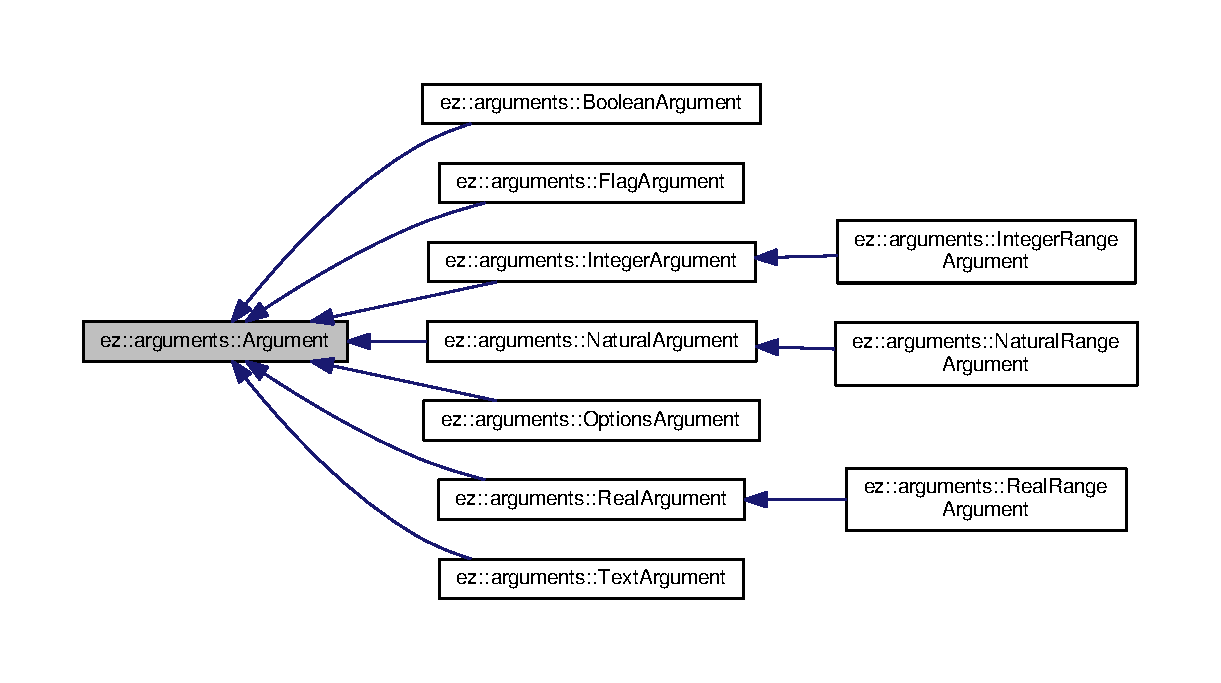
\includegraphics[width=350pt]{classez_1_1arguments_1_1Argument__inherit__graph}
\end{center}
\end{figure}
\subsection*{Public Member Functions}
\begin{DoxyCompactItemize}
\item 
\hyperlink{classez_1_1arguments_1_1Argument_af4799a33a85a7c1d11190f9f285b1117}{Argument} (text long\+\_\+label, char short\+\_\+label, text description, trigger\+\_\+t trigger=nullptr)
\item 
\hyperlink{classez_1_1arguments_1_1Argument_a86a267b41b09aba45426c36e4e92b097}{Argument} (text long\+\_\+label, text description, trigger\+\_\+t trigger=nullptr)
\item 
\mbox{\Hypertarget{classez_1_1arguments_1_1Argument_afc1595edacf1f3cd7f186fad18b8e518}\label{classez_1_1arguments_1_1Argument_afc1595edacf1f3cd7f186fad18b8e518}} 
text {\bfseries get\+\_\+long\+\_\+label} ()
\item 
\mbox{\Hypertarget{classez_1_1arguments_1_1Argument_a47ef11edb93c428268c19a7ab6c0aad4}\label{classez_1_1arguments_1_1Argument_a47ef11edb93c428268c19a7ab6c0aad4}} 
char {\bfseries get\+\_\+short\+\_\+label} ()
\item 
\mbox{\Hypertarget{classez_1_1arguments_1_1Argument_a71d439c68e7d0c9bca9f61bce30cfaa9}\label{classez_1_1arguments_1_1Argument_a71d439c68e7d0c9bca9f61bce30cfaa9}} 
text {\bfseries get\+\_\+description} ()
\item 
virtual void \hyperlink{classez_1_1arguments_1_1Argument_a7a4eb6a4d030416307584d8e77c2305a}{parse} (text \&s)=0
\item 
bool \hyperlink{classez_1_1arguments_1_1Argument_a049c9d70c97e990176247b5f4125f944}{is\+\_\+required} ()
\item 
\mbox{\Hypertarget{classez_1_1arguments_1_1Argument_a53a46cca0e608200f6b00df441c3e8b3}\label{classez_1_1arguments_1_1Argument_a53a46cca0e608200f6b00df441c3e8b3}} 
void {\bfseries set\+\_\+required} ()
\item 
\mbox{\Hypertarget{classez_1_1arguments_1_1Argument_ae358f87661528ecb27e838d7af17675a}\label{classez_1_1arguments_1_1Argument_ae358f87661528ecb27e838d7af17675a}} 
void {\bfseries set\+\_\+found} ()
\item 
\mbox{\Hypertarget{classez_1_1arguments_1_1Argument_a6e2f301f66312f1d45e2ade7921e7c42}\label{classez_1_1arguments_1_1Argument_a6e2f301f66312f1d45e2ade7921e7c42}} 
bool {\bfseries was\+\_\+found} ()
\item 
void \hyperlink{classez_1_1arguments_1_1Argument_a740f929b9c34fbcdc20e4105034bd369}{call\+\_\+trigger} ()
\end{DoxyCompactItemize}
\subsection*{Protected Attributes}
\begin{DoxyCompactItemize}
\item 
\mbox{\Hypertarget{classez_1_1arguments_1_1Argument_ac0857a07d17c78753b2609dc15b516b4}\label{classez_1_1arguments_1_1Argument_ac0857a07d17c78753b2609dc15b516b4}} 
text {\bfseries m\+\_\+long\+\_\+label}
\item 
\mbox{\Hypertarget{classez_1_1arguments_1_1Argument_ac21cad37b24aaa5e2bc281a197e76c21}\label{classez_1_1arguments_1_1Argument_ac21cad37b24aaa5e2bc281a197e76c21}} 
char {\bfseries m\+\_\+short\+\_\+label}
\item 
\mbox{\Hypertarget{classez_1_1arguments_1_1Argument_a85dccf7365873de6e4d18b80e78ee523}\label{classez_1_1arguments_1_1Argument_a85dccf7365873de6e4d18b80e78ee523}} 
text {\bfseries m\+\_\+description}
\item 
\mbox{\Hypertarget{classez_1_1arguments_1_1Argument_a8368ac83154f39c0082205460bad417c}\label{classez_1_1arguments_1_1Argument_a8368ac83154f39c0082205460bad417c}} 
bool {\bfseries m\+\_\+required}
\item 
\mbox{\Hypertarget{classez_1_1arguments_1_1Argument_aed5b51cd7d343c0016a815fddb081684}\label{classez_1_1arguments_1_1Argument_aed5b51cd7d343c0016a815fddb081684}} 
bool {\bfseries m\+\_\+found}
\item 
\mbox{\Hypertarget{classez_1_1arguments_1_1Argument_af5f2a640fe82cbcfcc2bb4121a6e3d50}\label{classez_1_1arguments_1_1Argument_af5f2a640fe82cbcfcc2bb4121a6e3d50}} 
trigger\+\_\+t {\bfseries m\+\_\+trigger}
\end{DoxyCompactItemize}
\subsection*{Friends}
\begin{DoxyCompactItemize}
\item 
\mbox{\Hypertarget{classez_1_1arguments_1_1Argument_a55c9e1ac006a645af402e3aee6b64e00}\label{classez_1_1arguments_1_1Argument_a55c9e1ac006a645af402e3aee6b64e00}} 
class {\bfseries Argument\+Parser}
\end{DoxyCompactItemize}


\subsection{Detailed Description}
default pattern to declare one class of argument 

\subsection{Constructor \& Destructor Documentation}
\mbox{\Hypertarget{classez_1_1arguments_1_1Argument_af4799a33a85a7c1d11190f9f285b1117}\label{classez_1_1arguments_1_1Argument_af4799a33a85a7c1d11190f9f285b1117}} 
\index{ez\+::arguments\+::\+Argument@{ez\+::arguments\+::\+Argument}!Argument@{Argument}}
\index{Argument@{Argument}!ez\+::arguments\+::\+Argument@{ez\+::arguments\+::\+Argument}}
\subsubsection{\texorpdfstring{Argument()}{Argument()}\hspace{0.1cm}{\footnotesize\ttfamily [1/2]}}
{\footnotesize\ttfamily ez\+::arguments\+::\+Argument\+::\+Argument (\begin{DoxyParamCaption}\item[{text}]{long\+\_\+label,  }\item[{char}]{short\+\_\+label,  }\item[{text}]{description,  }\item[{trigger\+\_\+t}]{trigger = {\ttfamily nullptr} }\end{DoxyParamCaption})\hspace{0.3cm}{\ttfamily [inline]}}

constructor with labels and description 
\begin{DoxyParams}{Parameters}
{\em ll} & label as long format (text) \\
\hline
{\em sl} & label as short format (char) \\
\hline
{\em d} & description \\
\hline
{\em tg} & trigger \\
\hline
\end{DoxyParams}
\mbox{\Hypertarget{classez_1_1arguments_1_1Argument_a86a267b41b09aba45426c36e4e92b097}\label{classez_1_1arguments_1_1Argument_a86a267b41b09aba45426c36e4e92b097}} 
\index{ez\+::arguments\+::\+Argument@{ez\+::arguments\+::\+Argument}!Argument@{Argument}}
\index{Argument@{Argument}!ez\+::arguments\+::\+Argument@{ez\+::arguments\+::\+Argument}}
\subsubsection{\texorpdfstring{Argument()}{Argument()}\hspace{0.1cm}{\footnotesize\ttfamily [2/2]}}
{\footnotesize\ttfamily ez\+::arguments\+::\+Argument\+::\+Argument (\begin{DoxyParamCaption}\item[{text}]{long\+\_\+label,  }\item[{text}]{description,  }\item[{trigger\+\_\+t}]{trigger = {\ttfamily nullptr} }\end{DoxyParamCaption})\hspace{0.3cm}{\ttfamily [inline]}}

constructor with labels and description but without short argument 
\begin{DoxyParams}{Parameters}
{\em ll} & label as long format (text) \\
\hline
{\em d} & description \\
\hline
{\em tg} & trigger \\
\hline
\end{DoxyParams}


\subsection{Member Function Documentation}
\mbox{\Hypertarget{classez_1_1arguments_1_1Argument_a740f929b9c34fbcdc20e4105034bd369}\label{classez_1_1arguments_1_1Argument_a740f929b9c34fbcdc20e4105034bd369}} 
\index{ez\+::arguments\+::\+Argument@{ez\+::arguments\+::\+Argument}!call\+\_\+trigger@{call\+\_\+trigger}}
\index{call\+\_\+trigger@{call\+\_\+trigger}!ez\+::arguments\+::\+Argument@{ez\+::arguments\+::\+Argument}}
\subsubsection{\texorpdfstring{call\+\_\+trigger()}{call\_trigger()}}
{\footnotesize\ttfamily void Argument\+::call\+\_\+trigger (\begin{DoxyParamCaption}{ }\end{DoxyParamCaption})}

call trigger if defined \mbox{\Hypertarget{classez_1_1arguments_1_1Argument_a049c9d70c97e990176247b5f4125f944}\label{classez_1_1arguments_1_1Argument_a049c9d70c97e990176247b5f4125f944}} 
\index{ez\+::arguments\+::\+Argument@{ez\+::arguments\+::\+Argument}!is\+\_\+required@{is\+\_\+required}}
\index{is\+\_\+required@{is\+\_\+required}!ez\+::arguments\+::\+Argument@{ez\+::arguments\+::\+Argument}}
\subsubsection{\texorpdfstring{is\+\_\+required()}{is\_required()}}
{\footnotesize\ttfamily bool ez\+::arguments\+::\+Argument\+::is\+\_\+required (\begin{DoxyParamCaption}{ }\end{DoxyParamCaption})\hspace{0.3cm}{\ttfamily [inline]}}

tells if this argument is required \mbox{\Hypertarget{classez_1_1arguments_1_1Argument_a7a4eb6a4d030416307584d8e77c2305a}\label{classez_1_1arguments_1_1Argument_a7a4eb6a4d030416307584d8e77c2305a}} 
\index{ez\+::arguments\+::\+Argument@{ez\+::arguments\+::\+Argument}!parse@{parse}}
\index{parse@{parse}!ez\+::arguments\+::\+Argument@{ez\+::arguments\+::\+Argument}}
\subsubsection{\texorpdfstring{parse()}{parse()}}
{\footnotesize\ttfamily virtual void ez\+::arguments\+::\+Argument\+::parse (\begin{DoxyParamCaption}\item[{text \&}]{s }\end{DoxyParamCaption})\hspace{0.3cm}{\ttfamily [pure virtual]}}

function used to parse argument argv\mbox{[}i\mbox{]}. for example if argument is \char`\"{}-\/-\/arg=value\char`\"{}, only the \char`\"{}value\char`\"{} part is given as the s parameter 

The documentation for this class was generated from the following files\+:\begin{DoxyCompactItemize}
\item 
src/version\+\_\+2018.\+06/arguments/argument.\+h\item 
src/version\+\_\+2018.\+06/arguments/argument.\+cpp\end{DoxyCompactItemize}

\hypertarget{classez_1_1arguments_1_1ArgumentParser}{}\section{ez\+:\+:arguments\+:\+:Argument\+Parser Class Reference}
\label{classez_1_1arguments_1_1ArgumentParser}\index{ez\+::arguments\+::\+Argument\+Parser@{ez\+::arguments\+::\+Argument\+Parser}}


{\ttfamily \#include $<$argument\+\_\+parser.\+h$>$}



Collaboration diagram for ez\+:\+:arguments\+:\+:Argument\+Parser\+:
\nopagebreak
\begin{figure}[H]
\begin{center}
\leavevmode
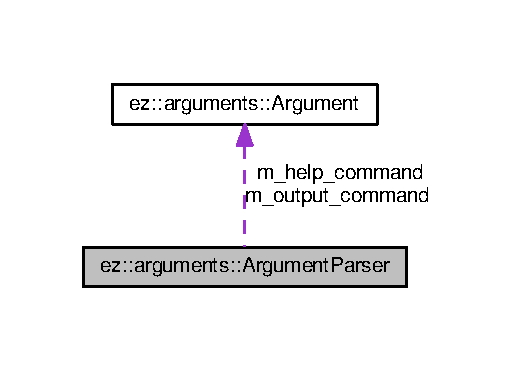
\includegraphics[width=247pt]{classez_1_1arguments_1_1ArgumentParser__coll__graph}
\end{center}
\end{figure}
\subsection*{Public Member Functions}
\begin{DoxyCompactItemize}
\item 
\hyperlink{classez_1_1arguments_1_1ArgumentParser_a30376da1d4671529adc656a9feee49e7}{Argument\+Parser} (text program\+\_\+name, text description, integer argc, char $\ast$argv\mbox{[}$\,$\mbox{]})
\item 
\mbox{\Hypertarget{classez_1_1arguments_1_1ArgumentParser_a04f55da04f5da57dec7ec34ca96c0ad1}\label{classez_1_1arguments_1_1ArgumentParser_a04f55da04f5da57dec7ec34ca96c0ad1}} 
void {\bfseries clean} ()
\item 
\hyperlink{classez_1_1arguments_1_1Argument}{Argument} $\ast$ \hyperlink{classez_1_1arguments_1_1ArgumentParser_aa14a00ee3b14e5d3c4ffa5b409d03274}{add} (\hyperlink{classez_1_1arguments_1_1Argument}{Argument} $\ast$arg)
\item 
\mbox{\Hypertarget{classez_1_1arguments_1_1ArgumentParser_a27ef9198a0bdd6c39a2897712ad402b4}\label{classez_1_1arguments_1_1ArgumentParser_a27ef9198a0bdd6c39a2897712ad402b4}} 
\hyperlink{classez_1_1arguments_1_1Argument}{Argument} $\ast$ {\bfseries add\+\_\+flag} (text long\+\_\+label, char short\+\_\+label, bool $\ast$value, text description, trigger\+\_\+t trigger=nullptr)
\item 
\mbox{\Hypertarget{classez_1_1arguments_1_1ArgumentParser_addffdc87f5acb326b7b64b5144395c42}\label{classez_1_1arguments_1_1ArgumentParser_addffdc87f5acb326b7b64b5144395c42}} 
\hyperlink{classez_1_1arguments_1_1Argument}{Argument} $\ast$ {\bfseries add\+\_\+boolean} (text long\+\_\+label, char short\+\_\+label, bool $\ast$value, text description, trigger\+\_\+t trigger=nullptr)
\item 
\mbox{\Hypertarget{classez_1_1arguments_1_1ArgumentParser_a83b1d6bcdb92004d97776a45ef8c17d7}\label{classez_1_1arguments_1_1ArgumentParser_a83b1d6bcdb92004d97776a45ef8c17d7}} 
\hyperlink{classez_1_1arguments_1_1Argument}{Argument} $\ast$ {\bfseries add\+\_\+integer} (text long\+\_\+label, char short\+\_\+label, integer $\ast$value, text description, trigger\+\_\+t trigger=nullptr)
\item 
\mbox{\Hypertarget{classez_1_1arguments_1_1ArgumentParser_abd978af3aacae6c47a019bad89b6afde}\label{classez_1_1arguments_1_1ArgumentParser_abd978af3aacae6c47a019bad89b6afde}} 
\hyperlink{classez_1_1arguments_1_1Argument}{Argument} $\ast$ {\bfseries add\+\_\+natural} (text long\+\_\+label, char short\+\_\+label, natural $\ast$value, text description, trigger\+\_\+t trigger=nullptr)
\item 
\mbox{\Hypertarget{classez_1_1arguments_1_1ArgumentParser_a849cbf117f92a755497fb37e206bf320}\label{classez_1_1arguments_1_1ArgumentParser_a849cbf117f92a755497fb37e206bf320}} 
\hyperlink{classez_1_1arguments_1_1Argument}{Argument} $\ast$ {\bfseries add\+\_\+real} (text long\+\_\+label, char short\+\_\+label, real $\ast$value, text description, trigger\+\_\+t trigger=nullptr)
\item 
\mbox{\Hypertarget{classez_1_1arguments_1_1ArgumentParser_ac90051ff2c8c2d6195336a733eb9441a}\label{classez_1_1arguments_1_1ArgumentParser_ac90051ff2c8c2d6195336a733eb9441a}} 
\hyperlink{classez_1_1arguments_1_1Argument}{Argument} $\ast$ {\bfseries add\+\_\+real\+\_\+range} (text long\+\_\+label, char short\+\_\+label, real $\ast$value, real mini, real maxi, text description, trigger\+\_\+t trigger=nullptr)
\item 
\mbox{\Hypertarget{classez_1_1arguments_1_1ArgumentParser_a28980f736205a085e955715079c82efa}\label{classez_1_1arguments_1_1ArgumentParser_a28980f736205a085e955715079c82efa}} 
\hyperlink{classez_1_1arguments_1_1Argument}{Argument} $\ast$ {\bfseries add\+\_\+integer\+\_\+range} (text long\+\_\+label, char short\+\_\+label, integer $\ast$value, integer mini, integer maxi, text description, trigger\+\_\+t trigger=nullptr)
\item 
\mbox{\Hypertarget{classez_1_1arguments_1_1ArgumentParser_acc784dd4d36c9682ee1e7f4d466ba0aa}\label{classez_1_1arguments_1_1ArgumentParser_acc784dd4d36c9682ee1e7f4d466ba0aa}} 
\hyperlink{classez_1_1arguments_1_1Argument}{Argument} $\ast$ {\bfseries add\+\_\+natural\+\_\+range} (text long\+\_\+label, char short\+\_\+label, natural $\ast$value, natural mini, natural maxi, text description, trigger\+\_\+t trigger=nullptr)
\item 
\mbox{\Hypertarget{classez_1_1arguments_1_1ArgumentParser_aabc8b35a31dd61bc334ae5d6213730fb}\label{classez_1_1arguments_1_1ArgumentParser_aabc8b35a31dd61bc334ae5d6213730fb}} 
\hyperlink{classez_1_1arguments_1_1Argument}{Argument} $\ast$ {\bfseries add\+\_\+text} (text long\+\_\+label, char short\+\_\+label, text $\ast$value, text description, trigger\+\_\+t trigger=nullptr)
\item 
\mbox{\Hypertarget{classez_1_1arguments_1_1ArgumentParser_a222f678cf331cc55c463386f1ff52519}\label{classez_1_1arguments_1_1ArgumentParser_a222f678cf331cc55c463386f1ff52519}} 
\hyperlink{classez_1_1arguments_1_1Argument}{Argument} $\ast$ {\bfseries add\+\_\+options} (text long\+\_\+label, char short\+\_\+label, natural $\ast$value, vector$<$ text $>$ \&options, text description, trigger\+\_\+t trigger=nullptr)
\item 
\mbox{\Hypertarget{classez_1_1arguments_1_1ArgumentParser_a9b8b290a07eac311665f91851b9d7b3d}\label{classez_1_1arguments_1_1ArgumentParser_a9b8b290a07eac311665f91851b9d7b3d}} 
natural {\bfseries nbr\+\_\+arguments} ()
\item 
void \hyperlink{classez_1_1arguments_1_1ArgumentParser_a740720f7b71d51c66b2211689cccf595}{parse} ()
\item 
void \hyperlink{classez_1_1arguments_1_1ArgumentParser_a19a161953f44e5f8c02ad53c4f9c660b}{report\+\_\+error} (exception \&e)
\end{DoxyCompactItemize}
\subsection*{Protected Member Functions}
\begin{DoxyCompactItemize}
\item 
void \hyperlink{classez_1_1arguments_1_1ArgumentParser_ac9a85ce0fb70333c02c19cb0310fe685}{print\+\_\+synopsis} (ostream \&out)
\item 
void \hyperlink{classez_1_1arguments_1_1ArgumentParser_a6bd8d09ae905811e2dc082f0574cbcbf}{print\+\_\+synopsis\+\_\+text} (ostream \&out, integer level, text s, natural length)
\item 
bool \hyperlink{classez_1_1arguments_1_1ArgumentParser_ace31a847d871c5c6c85db03716fa7047}{has\+\_\+to\+\_\+show\+\_\+synopsis} ()
\item 
void \hyperlink{classez_1_1arguments_1_1ArgumentParser_a0eedf118bbdf897606e5a0ebf6183102}{set\+\_\+has\+\_\+to\+\_\+show\+\_\+synopsis} (bool v)
\end{DoxyCompactItemize}
\subsection*{Protected Attributes}
\begin{DoxyCompactItemize}
\item 
\mbox{\Hypertarget{classez_1_1arguments_1_1ArgumentParser_a4658e78bae4efc91e96e5cc59c87d6b0}\label{classez_1_1arguments_1_1ArgumentParser_a4658e78bae4efc91e96e5cc59c87d6b0}} 
integer {\bfseries m\+\_\+argc}
\item 
\mbox{\Hypertarget{classez_1_1arguments_1_1ArgumentParser_acca763aec1698533801e9d5e6bf6449d}\label{classez_1_1arguments_1_1ArgumentParser_acca763aec1698533801e9d5e6bf6449d}} 
char $\ast$$\ast$ {\bfseries m\+\_\+argv}
\item 
\mbox{\Hypertarget{classez_1_1arguments_1_1ArgumentParser_ae08ee53ae5d4e14eff0a10fe9733d64e}\label{classez_1_1arguments_1_1ArgumentParser_ae08ee53ae5d4e14eff0a10fe9733d64e}} 
vector$<$ \hyperlink{classez_1_1arguments_1_1Argument}{Argument} $\ast$ $>$ {\bfseries m\+\_\+arguments}
\item 
\mbox{\Hypertarget{classez_1_1arguments_1_1ArgumentParser_a61af5842e72678ca60e2398b2d01a95e}\label{classez_1_1arguments_1_1ArgumentParser_a61af5842e72678ca60e2398b2d01a95e}} 
map$<$ text, \hyperlink{classez_1_1arguments_1_1Argument}{Argument} $\ast$ $>$ {\bfseries m\+\_\+map\+\_\+long}
\item 
\mbox{\Hypertarget{classez_1_1arguments_1_1ArgumentParser_ab97373f07e03f89aa32d46c60192bd52}\label{classez_1_1arguments_1_1ArgumentParser_ab97373f07e03f89aa32d46c60192bd52}} 
map$<$ char, \hyperlink{classez_1_1arguments_1_1Argument}{Argument} $\ast$ $>$ {\bfseries m\+\_\+map\+\_\+short}
\item 
\mbox{\Hypertarget{classez_1_1arguments_1_1ArgumentParser_a2d1acf92339872ca0f11f050c65fb54d}\label{classez_1_1arguments_1_1ArgumentParser_a2d1acf92339872ca0f11f050c65fb54d}} 
text {\bfseries m\+\_\+program\+\_\+name}
\item 
\mbox{\Hypertarget{classez_1_1arguments_1_1ArgumentParser_a47fc986ac8638c60e672d78a8643a61e}\label{classez_1_1arguments_1_1ArgumentParser_a47fc986ac8638c60e672d78a8643a61e}} 
text {\bfseries m\+\_\+program\+\_\+desc}
\item 
\mbox{\Hypertarget{classez_1_1arguments_1_1ArgumentParser_aba046f65a9ba3e8b8a241e70f962f2ca}\label{classez_1_1arguments_1_1ArgumentParser_aba046f65a9ba3e8b8a241e70f962f2ca}} 
\hyperlink{classez_1_1arguments_1_1Argument}{Argument} $\ast$ {\bfseries m\+\_\+help\+\_\+command}
\item 
\mbox{\Hypertarget{classez_1_1arguments_1_1ArgumentParser_a210b2bf9e058ee0f432cd50e1df3f62e}\label{classez_1_1arguments_1_1ArgumentParser_a210b2bf9e058ee0f432cd50e1df3f62e}} 
\hyperlink{classez_1_1arguments_1_1Argument}{Argument} $\ast$ {\bfseries m\+\_\+output\+\_\+command}
\item 
\mbox{\Hypertarget{classez_1_1arguments_1_1ArgumentParser_a37c866a8951dd8e493f7f87162304d1f}\label{classez_1_1arguments_1_1ArgumentParser_a37c866a8951dd8e493f7f87162304d1f}} 
bool {\bfseries m\+\_\+show\+\_\+synopsis}
\end{DoxyCompactItemize}


\subsection{Detailed Description}
main class to treat command line arguments of argv 

\subsection{Constructor \& Destructor Documentation}
\mbox{\Hypertarget{classez_1_1arguments_1_1ArgumentParser_a30376da1d4671529adc656a9feee49e7}\label{classez_1_1arguments_1_1ArgumentParser_a30376da1d4671529adc656a9feee49e7}} 
\index{ez\+::arguments\+::\+Argument\+Parser@{ez\+::arguments\+::\+Argument\+Parser}!Argument\+Parser@{Argument\+Parser}}
\index{Argument\+Parser@{Argument\+Parser}!ez\+::arguments\+::\+Argument\+Parser@{ez\+::arguments\+::\+Argument\+Parser}}
\subsubsection{\texorpdfstring{Argument\+Parser()}{ArgumentParser()}}
{\footnotesize\ttfamily Argument\+Parser\+::\+Argument\+Parser (\begin{DoxyParamCaption}\item[{text}]{program\+\_\+name,  }\item[{text}]{description,  }\item[{integer}]{argc,  }\item[{char $\ast$}]{argv\mbox{[}$\,$\mbox{]} }\end{DoxyParamCaption})}

constructor with argc and argv 
\begin{DoxyParams}{Parameters}
{\em program\+\_\+name} & name of program \\
\hline
{\em description} & description of what the program does \\
\hline
{\em argc} & number of command line arguments \\
\hline
{\em argv} & array of text of command line arguments \\
\hline
\end{DoxyParams}


\subsection{Member Function Documentation}
\mbox{\Hypertarget{classez_1_1arguments_1_1ArgumentParser_aa14a00ee3b14e5d3c4ffa5b409d03274}\label{classez_1_1arguments_1_1ArgumentParser_aa14a00ee3b14e5d3c4ffa5b409d03274}} 
\index{ez\+::arguments\+::\+Argument\+Parser@{ez\+::arguments\+::\+Argument\+Parser}!add@{add}}
\index{add@{add}!ez\+::arguments\+::\+Argument\+Parser@{ez\+::arguments\+::\+Argument\+Parser}}
\subsubsection{\texorpdfstring{add()}{add()}}
{\footnotesize\ttfamily \hyperlink{classez_1_1arguments_1_1Argument}{Argument} $\ast$ Argument\+Parser\+::add (\begin{DoxyParamCaption}\item[{\hyperlink{classez_1_1arguments_1_1Argument}{Argument} $\ast$}]{arg }\end{DoxyParamCaption})}

add new type of argument we check if the new argument to add does not have a short or long label equal to one of the existing arguments if it is a Label\+Argument we check if all options are different 
\begin{DoxyParams}{Parameters}
{\em arg} & pointer to new argument \\
\hline
\end{DoxyParams}
\mbox{\Hypertarget{classez_1_1arguments_1_1ArgumentParser_ace31a847d871c5c6c85db03716fa7047}\label{classez_1_1arguments_1_1ArgumentParser_ace31a847d871c5c6c85db03716fa7047}} 
\index{ez\+::arguments\+::\+Argument\+Parser@{ez\+::arguments\+::\+Argument\+Parser}!has\+\_\+to\+\_\+show\+\_\+synopsis@{has\+\_\+to\+\_\+show\+\_\+synopsis}}
\index{has\+\_\+to\+\_\+show\+\_\+synopsis@{has\+\_\+to\+\_\+show\+\_\+synopsis}!ez\+::arguments\+::\+Argument\+Parser@{ez\+::arguments\+::\+Argument\+Parser}}
\subsubsection{\texorpdfstring{has\+\_\+to\+\_\+show\+\_\+synopsis()}{has\_to\_show\_synopsis()}}
{\footnotesize\ttfamily bool ez\+::arguments\+::\+Argument\+Parser\+::has\+\_\+to\+\_\+show\+\_\+synopsis (\begin{DoxyParamCaption}{ }\end{DoxyParamCaption})\hspace{0.3cm}{\ttfamily [inline]}, {\ttfamily [protected]}}

return if we can print synopsis \mbox{\Hypertarget{classez_1_1arguments_1_1ArgumentParser_a740720f7b71d51c66b2211689cccf595}\label{classez_1_1arguments_1_1ArgumentParser_a740720f7b71d51c66b2211689cccf595}} 
\index{ez\+::arguments\+::\+Argument\+Parser@{ez\+::arguments\+::\+Argument\+Parser}!parse@{parse}}
\index{parse@{parse}!ez\+::arguments\+::\+Argument\+Parser@{ez\+::arguments\+::\+Argument\+Parser}}
\subsubsection{\texorpdfstring{parse()}{parse()}}
{\footnotesize\ttfamily void Argument\+Parser\+::parse (\begin{DoxyParamCaption}{ }\end{DoxyParamCaption})}

parse argv throw Exception in case of error \mbox{\Hypertarget{classez_1_1arguments_1_1ArgumentParser_ac9a85ce0fb70333c02c19cb0310fe685}\label{classez_1_1arguments_1_1ArgumentParser_ac9a85ce0fb70333c02c19cb0310fe685}} 
\index{ez\+::arguments\+::\+Argument\+Parser@{ez\+::arguments\+::\+Argument\+Parser}!print\+\_\+synopsis@{print\+\_\+synopsis}}
\index{print\+\_\+synopsis@{print\+\_\+synopsis}!ez\+::arguments\+::\+Argument\+Parser@{ez\+::arguments\+::\+Argument\+Parser}}
\subsubsection{\texorpdfstring{print\+\_\+synopsis()}{print\_synopsis()}}
{\footnotesize\ttfamily void Argument\+Parser\+::print\+\_\+synopsis (\begin{DoxyParamCaption}\item[{ostream \&}]{out }\end{DoxyParamCaption})\hspace{0.3cm}{\ttfamily [protected]}}

print synopsis of command 
\begin{DoxyParams}{Parameters}
{\em out} & output stream \\
\hline
{\em prog\+\_\+name} & name of program \\
\hline
{\em descr} & description of program (ex for ls \+: list directory contents) \\
\hline
\end{DoxyParams}
\mbox{\Hypertarget{classez_1_1arguments_1_1ArgumentParser_a6bd8d09ae905811e2dc082f0574cbcbf}\label{classez_1_1arguments_1_1ArgumentParser_a6bd8d09ae905811e2dc082f0574cbcbf}} 
\index{ez\+::arguments\+::\+Argument\+Parser@{ez\+::arguments\+::\+Argument\+Parser}!print\+\_\+synopsis\+\_\+text@{print\+\_\+synopsis\+\_\+text}}
\index{print\+\_\+synopsis\+\_\+text@{print\+\_\+synopsis\+\_\+text}!ez\+::arguments\+::\+Argument\+Parser@{ez\+::arguments\+::\+Argument\+Parser}}
\subsubsection{\texorpdfstring{print\+\_\+synopsis\+\_\+text()}{print\_synopsis\_text()}}
{\footnotesize\ttfamily void Argument\+Parser\+::print\+\_\+synopsis\+\_\+text (\begin{DoxyParamCaption}\item[{ostream \&}]{out,  }\item[{integer}]{level,  }\item[{text}]{s,  }\item[{natural}]{length }\end{DoxyParamCaption})\hspace{0.3cm}{\ttfamily [protected]}}

print text with given display length \mbox{\Hypertarget{classez_1_1arguments_1_1ArgumentParser_a19a161953f44e5f8c02ad53c4f9c660b}\label{classez_1_1arguments_1_1ArgumentParser_a19a161953f44e5f8c02ad53c4f9c660b}} 
\index{ez\+::arguments\+::\+Argument\+Parser@{ez\+::arguments\+::\+Argument\+Parser}!report\+\_\+error@{report\+\_\+error}}
\index{report\+\_\+error@{report\+\_\+error}!ez\+::arguments\+::\+Argument\+Parser@{ez\+::arguments\+::\+Argument\+Parser}}
\subsubsection{\texorpdfstring{report\+\_\+error()}{report\_error()}}
{\footnotesize\ttfamily void Argument\+Parser\+::report\+\_\+error (\begin{DoxyParamCaption}\item[{exception \&}]{e }\end{DoxyParamCaption})}

report error \mbox{\Hypertarget{classez_1_1arguments_1_1ArgumentParser_a0eedf118bbdf897606e5a0ebf6183102}\label{classez_1_1arguments_1_1ArgumentParser_a0eedf118bbdf897606e5a0ebf6183102}} 
\index{ez\+::arguments\+::\+Argument\+Parser@{ez\+::arguments\+::\+Argument\+Parser}!set\+\_\+has\+\_\+to\+\_\+show\+\_\+synopsis@{set\+\_\+has\+\_\+to\+\_\+show\+\_\+synopsis}}
\index{set\+\_\+has\+\_\+to\+\_\+show\+\_\+synopsis@{set\+\_\+has\+\_\+to\+\_\+show\+\_\+synopsis}!ez\+::arguments\+::\+Argument\+Parser@{ez\+::arguments\+::\+Argument\+Parser}}
\subsubsection{\texorpdfstring{set\+\_\+has\+\_\+to\+\_\+show\+\_\+synopsis()}{set\_has\_to\_show\_synopsis()}}
{\footnotesize\ttfamily void ez\+::arguments\+::\+Argument\+Parser\+::set\+\_\+has\+\_\+to\+\_\+show\+\_\+synopsis (\begin{DoxyParamCaption}\item[{bool}]{v }\end{DoxyParamCaption})\hspace{0.3cm}{\ttfamily [inline]}, {\ttfamily [protected]}}

tell if we can show synopsis 

The documentation for this class was generated from the following files\+:\begin{DoxyCompactItemize}
\item 
src/version\+\_\+2018.\+06/arguments/argument\+\_\+parser.\+h\item 
src/version\+\_\+2018.\+06/arguments/argument\+\_\+parser.\+cpp\end{DoxyCompactItemize}

\hypertarget{classez_1_1objects_1_1Array}{}\section{ez\+:\+:objects\+:\+:Array$<$ Data\+Type $>$ Class Template Reference}
\label{classez_1_1objects_1_1Array}\index{ez\+::objects\+::\+Array$<$ Data\+Type $>$@{ez\+::objects\+::\+Array$<$ Data\+Type $>$}}


{\ttfamily \#include $<$array.\+h$>$}



Inheritance diagram for ez\+:\+:objects\+:\+:Array$<$ Data\+Type $>$\+:
\nopagebreak
\begin{figure}[H]
\begin{center}
\leavevmode
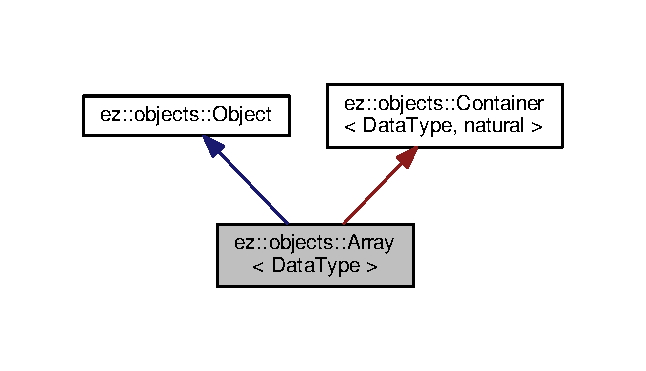
\includegraphics[width=310pt]{classez_1_1objects_1_1Array__inherit__graph}
\end{center}
\end{figure}


Collaboration diagram for ez\+:\+:objects\+:\+:Array$<$ Data\+Type $>$\+:
\nopagebreak
\begin{figure}[H]
\begin{center}
\leavevmode
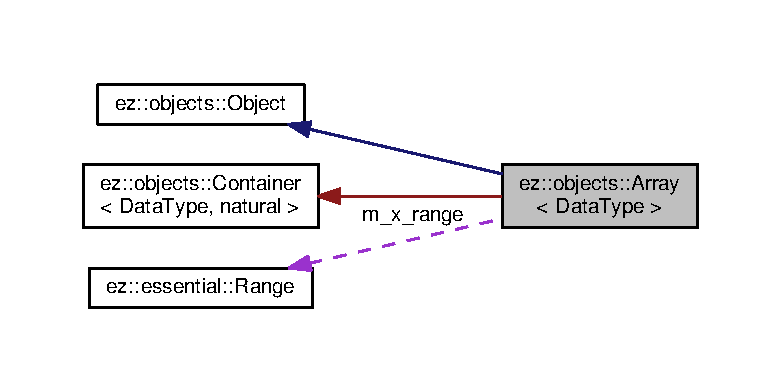
\includegraphics[width=350pt]{classez_1_1objects_1_1Array__coll__graph}
\end{center}
\end{figure}
\subsection*{Public Types}
\begin{DoxyCompactItemize}
\item 
\mbox{\Hypertarget{classez_1_1objects_1_1Array_aca95c7484bdd1ac9a1c80be3faa53ca4}\label{classez_1_1objects_1_1Array_aca95c7484bdd1ac9a1c80be3faa53ca4}} 
typedef \hyperlink{classez_1_1objects_1_1Array}{Array}$<$ Data\+Type $>$ {\bfseries self}
\item 
\mbox{\Hypertarget{classez_1_1objects_1_1Array_ad9930b3ad47ac4f2165436a1a2509a35}\label{classez_1_1objects_1_1Array_ad9930b3ad47ac4f2165436a1a2509a35}} 
typedef Data\+Type $\ast$ {\bfseries iterator}
\end{DoxyCompactItemize}
\subsection*{Public Member Functions}
\begin{DoxyCompactItemize}
\item 
\hyperlink{classez_1_1objects_1_1Array_a88ec7bab9f66c8fe7d97b4782a39ee84}{Array} ()
\item 
\hyperlink{classez_1_1objects_1_1Array_ab389febcc8d618c3b660fac1236898cb}{Array} (integer lo, integer hi)
\item 
\hyperlink{classez_1_1objects_1_1Array_a9ece37ee368a988a62351e8df1cdf220}{Array} (const \hyperlink{classez_1_1objects_1_1Array}{self} \&obj)
\item 
\hyperlink{classez_1_1objects_1_1Array_acc9a9ce3babaa4f1aa6d744304e2ccd0}{Array} (\hyperlink{classez_1_1essential_1_1Range}{Range} range)
\item 
\hyperlink{classez_1_1objects_1_1Array_a599e786f9331bd12c7eeef4a6e1ad043}{Array} (\hyperlink{classez_1_1essential_1_1Range}{Range} range, const std\+::initializer\+\_\+list$<$ Data\+Type $>$ \&l)
\item 
\hyperlink{classez_1_1objects_1_1Array_aa7998741d7bd1d2f92248846b39f5b2a}{$\sim$\+Array} ()
\item 
\hyperlink{classez_1_1objects_1_1Array}{self} \& \hyperlink{classez_1_1objects_1_1Array_a243625ca16cb6b1f7a7f68dc7a1922cf}{operator=} (const \hyperlink{classez_1_1objects_1_1Array}{self} \&obj)
\item 
void \hyperlink{classez_1_1objects_1_1Array_acdd164cad40bed068075550d943d19c2}{resize} (\hyperlink{classez_1_1essential_1_1Range}{Range} range)
\item 
bool \hyperlink{classez_1_1objects_1_1Array_a281b310f3f9f4140520b84c2315b1352}{is\+\_\+empty} ()
\item 
natural \hyperlink{classez_1_1objects_1_1Array_af3ac644ccc4058fb2e13797af274a3de}{size} ()
\item 
Data\+Type \& \hyperlink{classez_1_1objects_1_1Array_add86e335b90914397700e6f2cad45077}{operator\mbox{[}$\,$\mbox{]}} (integer n)
\item 
void \hyperlink{classez_1_1objects_1_1Array_a7f0707629712319837dc0cda091456b7}{print} (std\+::ostream \&stream) override
\item 
void \hyperlink{classez_1_1objects_1_1Array_a7f8b26dd8b96708d0a300a1f406ce336}{output} (std\+::ostream \&stream) override
\item 
void \hyperlink{classez_1_1objects_1_1Array_a438c2c6187dd5cce0dae9f303b34609c}{input} (std\+::istream \&stream) override
\item 
integer \hyperlink{classez_1_1objects_1_1Array_ac0d97a024e177f655b2f58981a68fcf8}{compare} (const \hyperlink{classez_1_1objects_1_1Object}{Object} \&y) override
\item 
\hyperlink{classez_1_1objects_1_1Object}{Object} $\ast$ \hyperlink{classez_1_1objects_1_1Array_a8618e73b6309573691b1fea690b8213a}{clone} () override
\item 
void \hyperlink{classez_1_1objects_1_1Array_a5ba81305951bfdef7454b3d3f11fc9d9}{fill} (Data\+Type value)
\item 
void \hyperlink{classez_1_1objects_1_1Array_aebeb0faa252f89e996f0b3a7250fa20b}{fill} (Data\+Type($\ast$genf)())
\item 
\mbox{\Hypertarget{classez_1_1objects_1_1Array_a935d5465ebb01aa797d16221cbd7a1ad}\label{classez_1_1objects_1_1Array_a935d5465ebb01aa797d16221cbd7a1ad}} 
{\footnotesize template$<$class Generator $>$ }\\void {\bfseries generate} (Generator g)
\item 
\mbox{\Hypertarget{classez_1_1objects_1_1Array_a13efb7e2473aebcb151b35245351644d}\label{classez_1_1objects_1_1Array_a13efb7e2473aebcb151b35245351644d}} 
iterator {\bfseries begin} ()
\item 
\mbox{\Hypertarget{classez_1_1objects_1_1Array_a66963da28335730f557d63b7b4793c7d}\label{classez_1_1objects_1_1Array_a66963da28335730f557d63b7b4793c7d}} 
iterator {\bfseries end} ()
\end{DoxyCompactItemize}
\subsection*{Protected Attributes}
\begin{DoxyCompactItemize}
\item 
\mbox{\Hypertarget{classez_1_1objects_1_1Array_a407695d81a0d4b0109d1238ff448fdbc}\label{classez_1_1objects_1_1Array_a407695d81a0d4b0109d1238ff448fdbc}} 
Data\+Type $\ast$ {\bfseries m\+\_\+data}
\item 
\mbox{\Hypertarget{classez_1_1objects_1_1Array_ad847a900350b845d2aee2325cb6c5441}\label{classez_1_1objects_1_1Array_ad847a900350b845d2aee2325cb6c5441}} 
\hyperlink{classez_1_1essential_1_1Range}{ez\+::essential\+::\+Range} {\bfseries m\+\_\+x\+\_\+range}
\item 
\mbox{\Hypertarget{classez_1_1objects_1_1Array_a53f49eb0bd13bf6aef934319cf4f11b8}\label{classez_1_1objects_1_1Array_a53f49eb0bd13bf6aef934319cf4f11b8}} 
natural {\bfseries m\+\_\+size}
\end{DoxyCompactItemize}
\subsection*{Friends}
\begin{DoxyCompactItemize}
\item 
\mbox{\Hypertarget{classez_1_1objects_1_1Array_aeada2177993d302d67110286099e5ccc}\label{classez_1_1objects_1_1Array_aeada2177993d302d67110286099e5ccc}} 
class {\bfseries Matrix2\+D$<$ Data\+Type $>$}
\end{DoxyCompactItemize}
\subsection*{Additional Inherited Members}


\subsection{Detailed Description}
\subsubsection*{template$<$class Data\+Type$>$\newline
class ez\+::objects\+::\+Array$<$ Data\+Type $>$}

Generic class that represents an array of Data\+Type values. The indexes of the array are taken in the Range\+Type interval which has integer type. For example we can represent an array of real numbers with indexes that range from -\/3 to 10 by the following declaration\+: {\ttfamily Array$<$real$>$ a(-\/3,10)} 

\subsection{Constructor \& Destructor Documentation}
\mbox{\Hypertarget{classez_1_1objects_1_1Array_a88ec7bab9f66c8fe7d97b4782a39ee84}\label{classez_1_1objects_1_1Array_a88ec7bab9f66c8fe7d97b4782a39ee84}} 
\index{ez\+::objects\+::\+Array@{ez\+::objects\+::\+Array}!Array@{Array}}
\index{Array@{Array}!ez\+::objects\+::\+Array@{ez\+::objects\+::\+Array}}
\subsubsection{\texorpdfstring{Array()}{Array()}\hspace{0.1cm}{\footnotesize\ttfamily [1/5]}}
{\footnotesize\ttfamily template$<$class Data\+Type$>$ \\
\hyperlink{classez_1_1objects_1_1Array}{ez\+::objects\+::\+Array}$<$ Data\+Type $>$\+::\hyperlink{classez_1_1objects_1_1Array}{Array} (\begin{DoxyParamCaption}{ }\end{DoxyParamCaption})\hspace{0.3cm}{\ttfamily [inline]}}

Default constructor \mbox{\Hypertarget{classez_1_1objects_1_1Array_ab389febcc8d618c3b660fac1236898cb}\label{classez_1_1objects_1_1Array_ab389febcc8d618c3b660fac1236898cb}} 
\index{ez\+::objects\+::\+Array@{ez\+::objects\+::\+Array}!Array@{Array}}
\index{Array@{Array}!ez\+::objects\+::\+Array@{ez\+::objects\+::\+Array}}
\subsubsection{\texorpdfstring{Array()}{Array()}\hspace{0.1cm}{\footnotesize\ttfamily [2/5]}}
{\footnotesize\ttfamily template$<$class Data\+Type$>$ \\
\hyperlink{classez_1_1objects_1_1Array}{ez\+::objects\+::\+Array}$<$ Data\+Type $>$\+::\hyperlink{classez_1_1objects_1_1Array}{Array} (\begin{DoxyParamCaption}\item[{integer}]{lo,  }\item[{integer}]{hi }\end{DoxyParamCaption})\hspace{0.3cm}{\ttfamily [inline]}}

Constructor given minimum and maximum index. 
\begin{DoxyParams}{Parameters}
{\em lo} & minimum index value \\
\hline
{\em hi} & maximum index value \\
\hline
\end{DoxyParams}
\mbox{\Hypertarget{classez_1_1objects_1_1Array_a9ece37ee368a988a62351e8df1cdf220}\label{classez_1_1objects_1_1Array_a9ece37ee368a988a62351e8df1cdf220}} 
\index{ez\+::objects\+::\+Array@{ez\+::objects\+::\+Array}!Array@{Array}}
\index{Array@{Array}!ez\+::objects\+::\+Array@{ez\+::objects\+::\+Array}}
\subsubsection{\texorpdfstring{Array()}{Array()}\hspace{0.1cm}{\footnotesize\ttfamily [3/5]}}
{\footnotesize\ttfamily template$<$class Data\+Type$>$ \\
\hyperlink{classez_1_1objects_1_1Array}{ez\+::objects\+::\+Array}$<$ Data\+Type $>$\+::\hyperlink{classez_1_1objects_1_1Array}{Array} (\begin{DoxyParamCaption}\item[{const \hyperlink{classez_1_1objects_1_1Array}{self} \&}]{obj }\end{DoxyParamCaption})\hspace{0.3cm}{\ttfamily [inline]}}

Copy constructor 
\begin{DoxyParams}{Parameters}
{\em obj} & reference to existing array \\
\hline
\end{DoxyParams}
\mbox{\Hypertarget{classez_1_1objects_1_1Array_acc9a9ce3babaa4f1aa6d744304e2ccd0}\label{classez_1_1objects_1_1Array_acc9a9ce3babaa4f1aa6d744304e2ccd0}} 
\index{ez\+::objects\+::\+Array@{ez\+::objects\+::\+Array}!Array@{Array}}
\index{Array@{Array}!ez\+::objects\+::\+Array@{ez\+::objects\+::\+Array}}
\subsubsection{\texorpdfstring{Array()}{Array()}\hspace{0.1cm}{\footnotesize\ttfamily [4/5]}}
{\footnotesize\ttfamily template$<$class Data\+Type$>$ \\
\hyperlink{classez_1_1objects_1_1Array}{ez\+::objects\+::\+Array}$<$ Data\+Type $>$\+::\hyperlink{classez_1_1objects_1_1Array}{Array} (\begin{DoxyParamCaption}\item[{\hyperlink{classez_1_1essential_1_1Range}{Range}}]{range }\end{DoxyParamCaption})\hspace{0.3cm}{\ttfamily [inline]}}

Constructor given range and initializer 
\begin{DoxyParams}{Parameters}
{\em range} & range of index \\
\hline
\end{DoxyParams}
\mbox{\Hypertarget{classez_1_1objects_1_1Array_a599e786f9331bd12c7eeef4a6e1ad043}\label{classez_1_1objects_1_1Array_a599e786f9331bd12c7eeef4a6e1ad043}} 
\index{ez\+::objects\+::\+Array@{ez\+::objects\+::\+Array}!Array@{Array}}
\index{Array@{Array}!ez\+::objects\+::\+Array@{ez\+::objects\+::\+Array}}
\subsubsection{\texorpdfstring{Array()}{Array()}\hspace{0.1cm}{\footnotesize\ttfamily [5/5]}}
{\footnotesize\ttfamily template$<$class Data\+Type$>$ \\
\hyperlink{classez_1_1objects_1_1Array}{ez\+::objects\+::\+Array}$<$ Data\+Type $>$\+::\hyperlink{classez_1_1objects_1_1Array}{Array} (\begin{DoxyParamCaption}\item[{\hyperlink{classez_1_1essential_1_1Range}{Range}}]{range,  }\item[{const std\+::initializer\+\_\+list$<$ Data\+Type $>$ \&}]{l }\end{DoxyParamCaption})\hspace{0.3cm}{\ttfamily [inline]}}

Constructor given range and initializer 
\begin{DoxyParams}{Parameters}
{\em range} & range of index \\
\hline
{\em l} & list of values for initialization \\
\hline
\end{DoxyParams}
\mbox{\Hypertarget{classez_1_1objects_1_1Array_aa7998741d7bd1d2f92248846b39f5b2a}\label{classez_1_1objects_1_1Array_aa7998741d7bd1d2f92248846b39f5b2a}} 
\index{ez\+::objects\+::\+Array@{ez\+::objects\+::\+Array}!````~Array@{$\sim$\+Array}}
\index{````~Array@{$\sim$\+Array}!ez\+::objects\+::\+Array@{ez\+::objects\+::\+Array}}
\subsubsection{\texorpdfstring{$\sim$\+Array()}{~Array()}}
{\footnotesize\ttfamily template$<$class Data\+Type$>$ \\
\hyperlink{classez_1_1objects_1_1Array}{ez\+::objects\+::\+Array}$<$ Data\+Type $>$\+::$\sim$\hyperlink{classez_1_1objects_1_1Array}{Array} (\begin{DoxyParamCaption}{ }\end{DoxyParamCaption})\hspace{0.3cm}{\ttfamily [inline]}}

Destructor 

\subsection{Member Function Documentation}
\mbox{\Hypertarget{classez_1_1objects_1_1Array_a8618e73b6309573691b1fea690b8213a}\label{classez_1_1objects_1_1Array_a8618e73b6309573691b1fea690b8213a}} 
\index{ez\+::objects\+::\+Array@{ez\+::objects\+::\+Array}!clone@{clone}}
\index{clone@{clone}!ez\+::objects\+::\+Array@{ez\+::objects\+::\+Array}}
\subsubsection{\texorpdfstring{clone()}{clone()}}
{\footnotesize\ttfamily template$<$class Data\+Type$>$ \\
\hyperlink{classez_1_1objects_1_1Object}{Object}$\ast$ \hyperlink{classez_1_1objects_1_1Array}{ez\+::objects\+::\+Array}$<$ Data\+Type $>$\+::clone (\begin{DoxyParamCaption}{ }\end{DoxyParamCaption})\hspace{0.3cm}{\ttfamily [inline]}, {\ttfamily [override]}, {\ttfamily [virtual]}}

Create and return copy of this object 

Reimplemented from \hyperlink{classez_1_1objects_1_1Object_acf444b2581d898eb4b8c92c2d5865c9e}{ez\+::objects\+::\+Object}.

\mbox{\Hypertarget{classez_1_1objects_1_1Array_ac0d97a024e177f655b2f58981a68fcf8}\label{classez_1_1objects_1_1Array_ac0d97a024e177f655b2f58981a68fcf8}} 
\index{ez\+::objects\+::\+Array@{ez\+::objects\+::\+Array}!compare@{compare}}
\index{compare@{compare}!ez\+::objects\+::\+Array@{ez\+::objects\+::\+Array}}
\subsubsection{\texorpdfstring{compare()}{compare()}}
{\footnotesize\ttfamily template$<$class Data\+Type$>$ \\
integer \hyperlink{classez_1_1objects_1_1Array}{ez\+::objects\+::\+Array}$<$ Data\+Type $>$\+::compare (\begin{DoxyParamCaption}\item[{const \hyperlink{classez_1_1objects_1_1Object}{Object} \&}]{y }\end{DoxyParamCaption})\hspace{0.3cm}{\ttfamily [inline]}, {\ttfamily [override]}, {\ttfamily [virtual]}}

Overloading of Compare method to Compare two arrays The arrays are equal if they have the same size and that the elements are identical 

Reimplemented from \hyperlink{classez_1_1objects_1_1Object_aca311d389dffa204e425463145f4e1e6}{ez\+::objects\+::\+Object}.

\mbox{\Hypertarget{classez_1_1objects_1_1Array_a5ba81305951bfdef7454b3d3f11fc9d9}\label{classez_1_1objects_1_1Array_a5ba81305951bfdef7454b3d3f11fc9d9}} 
\index{ez\+::objects\+::\+Array@{ez\+::objects\+::\+Array}!fill@{fill}}
\index{fill@{fill}!ez\+::objects\+::\+Array@{ez\+::objects\+::\+Array}}
\subsubsection{\texorpdfstring{fill()}{fill()}\hspace{0.1cm}{\footnotesize\ttfamily [1/2]}}
{\footnotesize\ttfamily template$<$class Data\+Type$>$ \\
void \hyperlink{classez_1_1objects_1_1Array}{ez\+::objects\+::\+Array}$<$ Data\+Type $>$\+::fill (\begin{DoxyParamCaption}\item[{Data\+Type}]{value }\end{DoxyParamCaption})\hspace{0.3cm}{\ttfamily [inline]}}

Fill array with given value 
\begin{DoxyParams}{Parameters}
{\em value} & value that will be assigned to each element \\
\hline
\end{DoxyParams}
\mbox{\Hypertarget{classez_1_1objects_1_1Array_aebeb0faa252f89e996f0b3a7250fa20b}\label{classez_1_1objects_1_1Array_aebeb0faa252f89e996f0b3a7250fa20b}} 
\index{ez\+::objects\+::\+Array@{ez\+::objects\+::\+Array}!fill@{fill}}
\index{fill@{fill}!ez\+::objects\+::\+Array@{ez\+::objects\+::\+Array}}
\subsubsection{\texorpdfstring{fill()}{fill()}\hspace{0.1cm}{\footnotesize\ttfamily [2/2]}}
{\footnotesize\ttfamily template$<$class Data\+Type$>$ \\
void \hyperlink{classez_1_1objects_1_1Array}{ez\+::objects\+::\+Array}$<$ Data\+Type $>$\+::fill (\begin{DoxyParamCaption}\item[{Data\+Type($\ast$)()}]{genf }\end{DoxyParamCaption})\hspace{0.3cm}{\ttfamily [inline]}}

Fill array using a generator 
\begin{DoxyParams}{Parameters}
{\em genf} & pointer to generator \\
\hline
\end{DoxyParams}
\mbox{\Hypertarget{classez_1_1objects_1_1Array_a438c2c6187dd5cce0dae9f303b34609c}\label{classez_1_1objects_1_1Array_a438c2c6187dd5cce0dae9f303b34609c}} 
\index{ez\+::objects\+::\+Array@{ez\+::objects\+::\+Array}!input@{input}}
\index{input@{input}!ez\+::objects\+::\+Array@{ez\+::objects\+::\+Array}}
\subsubsection{\texorpdfstring{input()}{input()}}
{\footnotesize\ttfamily template$<$class Data\+Type$>$ \\
void \hyperlink{classez_1_1objects_1_1Array}{ez\+::objects\+::\+Array}$<$ Data\+Type $>$\+::input (\begin{DoxyParamCaption}\item[{std\+::istream \&}]{stream }\end{DoxyParamCaption})\hspace{0.3cm}{\ttfamily [inline]}, {\ttfamily [override]}, {\ttfamily [virtual]}}

overloading of output method to unserialize object 

Reimplemented from \hyperlink{classez_1_1objects_1_1Object_a878bdc53b7f16fda6fa15dab214c4b6a}{ez\+::objects\+::\+Object}.

\mbox{\Hypertarget{classez_1_1objects_1_1Array_a281b310f3f9f4140520b84c2315b1352}\label{classez_1_1objects_1_1Array_a281b310f3f9f4140520b84c2315b1352}} 
\index{ez\+::objects\+::\+Array@{ez\+::objects\+::\+Array}!is\+\_\+empty@{is\+\_\+empty}}
\index{is\+\_\+empty@{is\+\_\+empty}!ez\+::objects\+::\+Array@{ez\+::objects\+::\+Array}}
\subsubsection{\texorpdfstring{is\+\_\+empty()}{is\_empty()}}
{\footnotesize\ttfamily template$<$class Data\+Type$>$ \\
bool \hyperlink{classez_1_1objects_1_1Array}{ez\+::objects\+::\+Array}$<$ Data\+Type $>$\+::is\+\_\+empty (\begin{DoxyParamCaption}{ }\end{DoxyParamCaption})\hspace{0.3cm}{\ttfamily [inline]}, {\ttfamily [virtual]}}

Return true if array is empty, false otherwise 

Implements \hyperlink{classez_1_1objects_1_1Container_a205eb4f8a4fe967d425fdf04e5db5f93}{ez\+::objects\+::\+Container$<$ Data\+Type, natural $>$}.

\mbox{\Hypertarget{classez_1_1objects_1_1Array_a243625ca16cb6b1f7a7f68dc7a1922cf}\label{classez_1_1objects_1_1Array_a243625ca16cb6b1f7a7f68dc7a1922cf}} 
\index{ez\+::objects\+::\+Array@{ez\+::objects\+::\+Array}!operator=@{operator=}}
\index{operator=@{operator=}!ez\+::objects\+::\+Array@{ez\+::objects\+::\+Array}}
\subsubsection{\texorpdfstring{operator=()}{operator=()}}
{\footnotesize\ttfamily template$<$class Data\+Type$>$ \\
\hyperlink{classez_1_1objects_1_1Array}{self}\& \hyperlink{classez_1_1objects_1_1Array}{ez\+::objects\+::\+Array}$<$ Data\+Type $>$\+::operator= (\begin{DoxyParamCaption}\item[{const \hyperlink{classez_1_1objects_1_1Array}{self} \&}]{obj }\end{DoxyParamCaption})\hspace{0.3cm}{\ttfamily [inline]}}

Assignment operator. 
\begin{DoxyParams}{Parameters}
{\em obj} & reference to existing array \\
\hline
\end{DoxyParams}
\mbox{\Hypertarget{classez_1_1objects_1_1Array_add86e335b90914397700e6f2cad45077}\label{classez_1_1objects_1_1Array_add86e335b90914397700e6f2cad45077}} 
\index{ez\+::objects\+::\+Array@{ez\+::objects\+::\+Array}!operator\mbox{[}\mbox{]}@{operator[]}}
\index{operator\mbox{[}\mbox{]}@{operator[]}!ez\+::objects\+::\+Array@{ez\+::objects\+::\+Array}}
\subsubsection{\texorpdfstring{operator[]()}{operator[]()}}
{\footnotesize\ttfamily template$<$class Data\+Type$>$ \\
Data\+Type\& \hyperlink{classez_1_1objects_1_1Array}{ez\+::objects\+::\+Array}$<$ Data\+Type $>$\+::operator\mbox{[}$\,$\mbox{]} (\begin{DoxyParamCaption}\item[{integer}]{n }\end{DoxyParamCaption})\hspace{0.3cm}{\ttfamily [inline]}}

Get access to value using index 
\begin{DoxyParams}{Parameters}
{\em index} & of the value \\
\hline
\end{DoxyParams}
\begin{DoxyReturn}{Returns}
reference to value 
\end{DoxyReturn}
\mbox{\Hypertarget{classez_1_1objects_1_1Array_a7f8b26dd8b96708d0a300a1f406ce336}\label{classez_1_1objects_1_1Array_a7f8b26dd8b96708d0a300a1f406ce336}} 
\index{ez\+::objects\+::\+Array@{ez\+::objects\+::\+Array}!output@{output}}
\index{output@{output}!ez\+::objects\+::\+Array@{ez\+::objects\+::\+Array}}
\subsubsection{\texorpdfstring{output()}{output()}}
{\footnotesize\ttfamily template$<$class Data\+Type$>$ \\
void \hyperlink{classez_1_1objects_1_1Array}{ez\+::objects\+::\+Array}$<$ Data\+Type $>$\+::output (\begin{DoxyParamCaption}\item[{std\+::ostream \&}]{stream }\end{DoxyParamCaption})\hspace{0.3cm}{\ttfamily [inline]}, {\ttfamily [override]}, {\ttfamily [virtual]}}

overloading of output method to serialize object 

Reimplemented from \hyperlink{classez_1_1objects_1_1Object_a0fdfe18e6c35d6b0d7e7a01265aded15}{ez\+::objects\+::\+Object}.

\mbox{\Hypertarget{classez_1_1objects_1_1Array_a7f0707629712319837dc0cda091456b7}\label{classez_1_1objects_1_1Array_a7f0707629712319837dc0cda091456b7}} 
\index{ez\+::objects\+::\+Array@{ez\+::objects\+::\+Array}!print@{print}}
\index{print@{print}!ez\+::objects\+::\+Array@{ez\+::objects\+::\+Array}}
\subsubsection{\texorpdfstring{print()}{print()}}
{\footnotesize\ttfamily template$<$class Data\+Type$>$ \\
void \hyperlink{classez_1_1objects_1_1Array}{ez\+::objects\+::\+Array}$<$ Data\+Type $>$\+::print (\begin{DoxyParamCaption}\item[{std\+::ostream \&}]{stream }\end{DoxyParamCaption})\hspace{0.3cm}{\ttfamily [inline]}, {\ttfamily [override]}, {\ttfamily [virtual]}}

overloading of print method of class \hyperlink{classez_1_1objects_1_1Object}{Object} 

Reimplemented from \hyperlink{classez_1_1objects_1_1Object_a9e20f39a78163f67f000576149d858b3}{ez\+::objects\+::\+Object}.

\mbox{\Hypertarget{classez_1_1objects_1_1Array_acdd164cad40bed068075550d943d19c2}\label{classez_1_1objects_1_1Array_acdd164cad40bed068075550d943d19c2}} 
\index{ez\+::objects\+::\+Array@{ez\+::objects\+::\+Array}!resize@{resize}}
\index{resize@{resize}!ez\+::objects\+::\+Array@{ez\+::objects\+::\+Array}}
\subsubsection{\texorpdfstring{resize()}{resize()}}
{\footnotesize\ttfamily template$<$class Data\+Type$>$ \\
void \hyperlink{classez_1_1objects_1_1Array}{ez\+::objects\+::\+Array}$<$ Data\+Type $>$\+::resize (\begin{DoxyParamCaption}\item[{\hyperlink{classez_1_1essential_1_1Range}{Range}}]{range }\end{DoxyParamCaption})\hspace{0.3cm}{\ttfamily [inline]}}

modify size of array 
\begin{DoxyParams}{Parameters}
{\em range} & new Range for the array \\
\hline
\end{DoxyParams}
\mbox{\Hypertarget{classez_1_1objects_1_1Array_af3ac644ccc4058fb2e13797af274a3de}\label{classez_1_1objects_1_1Array_af3ac644ccc4058fb2e13797af274a3de}} 
\index{ez\+::objects\+::\+Array@{ez\+::objects\+::\+Array}!size@{size}}
\index{size@{size}!ez\+::objects\+::\+Array@{ez\+::objects\+::\+Array}}
\subsubsection{\texorpdfstring{size()}{size()}}
{\footnotesize\ttfamily template$<$class Data\+Type$>$ \\
natural \hyperlink{classez_1_1objects_1_1Array}{ez\+::objects\+::\+Array}$<$ Data\+Type $>$\+::size (\begin{DoxyParamCaption}{ }\end{DoxyParamCaption})\hspace{0.3cm}{\ttfamily [inline]}, {\ttfamily [virtual]}}

Return the number of elements of the array 

Implements \hyperlink{classez_1_1objects_1_1Container_affd294810c6c29530d1d1e3c2151ad28}{ez\+::objects\+::\+Container$<$ Data\+Type, natural $>$}.



The documentation for this class was generated from the following file\+:\begin{DoxyCompactItemize}
\item 
src/version\+\_\+2018.\+06/objects/array.\+h\end{DoxyCompactItemize}

\hypertarget{classez_1_1logging_1_1BaseLogger}{}\section{ez\+:\+:logging\+:\+:Base\+Logger Class Reference}
\label{classez_1_1logging_1_1BaseLogger}\index{ez\+::logging\+::\+Base\+Logger@{ez\+::logging\+::\+Base\+Logger}}


{\ttfamily \#include $<$logger.\+h$>$}



Inheritance diagram for ez\+:\+:logging\+:\+:Base\+Logger\+:
\nopagebreak
\begin{figure}[H]
\begin{center}
\leavevmode
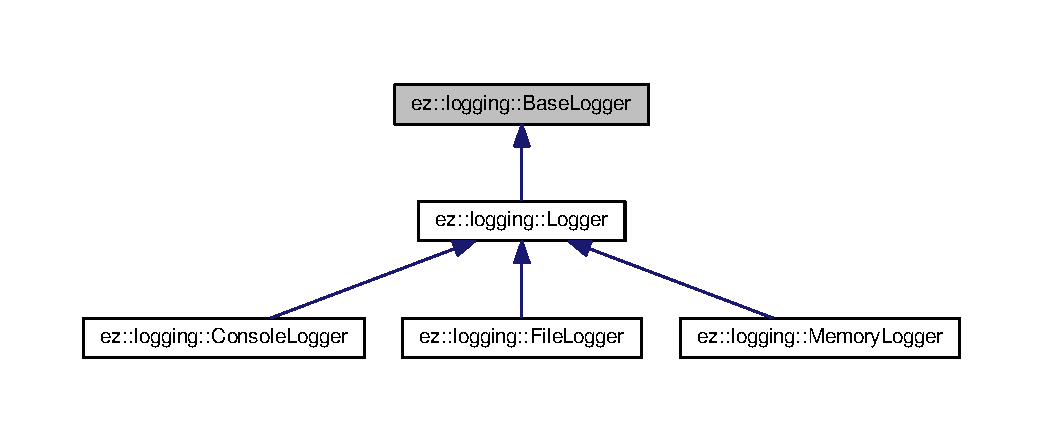
\includegraphics[width=350pt]{classez_1_1logging_1_1BaseLogger__inherit__graph}
\end{center}
\end{figure}
\subsection*{Public Member Functions}
\begin{DoxyCompactItemize}
\item 
\hyperlink{classez_1_1logging_1_1BaseLogger_ac0f5809baaacc153b6b51eb1a028127b}{Base\+Logger} ()
\item 
virtual \hyperlink{classez_1_1logging_1_1BaseLogger_a8f3ff996b9cd518dc53760ece4083813}{$\sim$\+Base\+Logger} ()
\item 
virtual void \hyperlink{classez_1_1logging_1_1BaseLogger_a508a25672c704ec73260978b7f17dd13}{set\+\_\+record\+\_\+level} (integer n)=0
\item 
virtual void \hyperlink{classez_1_1logging_1_1BaseLogger_a2b9ecfbaff4e53d15b3b8bedd53ea2f8}{set\+\_\+verbose\+\_\+level} (integer n)=0
\item 
virtual void \hyperlink{classez_1_1logging_1_1BaseLogger_a1cad8cfe8029ecd0360573b3dd4a0543}{print\+\_\+ln} ()=0
\end{DoxyCompactItemize}


\subsection{Detailed Description}
Base class for \hyperlink{classez_1_1logging_1_1Logger}{Logger} used to define kind of iomanip operations for Loggers 

\subsection{Constructor \& Destructor Documentation}
\mbox{\Hypertarget{classez_1_1logging_1_1BaseLogger_ac0f5809baaacc153b6b51eb1a028127b}\label{classez_1_1logging_1_1BaseLogger_ac0f5809baaacc153b6b51eb1a028127b}} 
\index{ez\+::logging\+::\+Base\+Logger@{ez\+::logging\+::\+Base\+Logger}!Base\+Logger@{Base\+Logger}}
\index{Base\+Logger@{Base\+Logger}!ez\+::logging\+::\+Base\+Logger@{ez\+::logging\+::\+Base\+Logger}}
\subsubsection{\texorpdfstring{Base\+Logger()}{BaseLogger()}}
{\footnotesize\ttfamily ez\+::logging\+::\+Base\+Logger\+::\+Base\+Logger (\begin{DoxyParamCaption}{ }\end{DoxyParamCaption})\hspace{0.3cm}{\ttfamily [inline]}}

default constructor \mbox{\Hypertarget{classez_1_1logging_1_1BaseLogger_a8f3ff996b9cd518dc53760ece4083813}\label{classez_1_1logging_1_1BaseLogger_a8f3ff996b9cd518dc53760ece4083813}} 
\index{ez\+::logging\+::\+Base\+Logger@{ez\+::logging\+::\+Base\+Logger}!````~Base\+Logger@{$\sim$\+Base\+Logger}}
\index{````~Base\+Logger@{$\sim$\+Base\+Logger}!ez\+::logging\+::\+Base\+Logger@{ez\+::logging\+::\+Base\+Logger}}
\subsubsection{\texorpdfstring{$\sim$\+Base\+Logger()}{~BaseLogger()}}
{\footnotesize\ttfamily virtual ez\+::logging\+::\+Base\+Logger\+::$\sim$\+Base\+Logger (\begin{DoxyParamCaption}{ }\end{DoxyParamCaption})\hspace{0.3cm}{\ttfamily [inline]}, {\ttfamily [virtual]}}

destructor 

\subsection{Member Function Documentation}
\mbox{\Hypertarget{classez_1_1logging_1_1BaseLogger_a1cad8cfe8029ecd0360573b3dd4a0543}\label{classez_1_1logging_1_1BaseLogger_a1cad8cfe8029ecd0360573b3dd4a0543}} 
\index{ez\+::logging\+::\+Base\+Logger@{ez\+::logging\+::\+Base\+Logger}!print\+\_\+ln@{print\+\_\+ln}}
\index{print\+\_\+ln@{print\+\_\+ln}!ez\+::logging\+::\+Base\+Logger@{ez\+::logging\+::\+Base\+Logger}}
\subsubsection{\texorpdfstring{print\+\_\+ln()}{print\_ln()}}
{\footnotesize\ttfamily virtual void ez\+::logging\+::\+Base\+Logger\+::print\+\_\+ln (\begin{DoxyParamCaption}{ }\end{DoxyParamCaption})\hspace{0.3cm}{\ttfamily [pure virtual]}}

virtual function used to print new line 

Implemented in \hyperlink{classez_1_1logging_1_1Logger_ab8e5b19223eca4b3af5ff7df2db607b7}{ez\+::logging\+::\+Logger}.

\mbox{\Hypertarget{classez_1_1logging_1_1BaseLogger_a508a25672c704ec73260978b7f17dd13}\label{classez_1_1logging_1_1BaseLogger_a508a25672c704ec73260978b7f17dd13}} 
\index{ez\+::logging\+::\+Base\+Logger@{ez\+::logging\+::\+Base\+Logger}!set\+\_\+record\+\_\+level@{set\+\_\+record\+\_\+level}}
\index{set\+\_\+record\+\_\+level@{set\+\_\+record\+\_\+level}!ez\+::logging\+::\+Base\+Logger@{ez\+::logging\+::\+Base\+Logger}}
\subsubsection{\texorpdfstring{set\+\_\+record\+\_\+level()}{set\_record\_level()}}
{\footnotesize\ttfamily virtual void ez\+::logging\+::\+Base\+Logger\+::set\+\_\+record\+\_\+level (\begin{DoxyParamCaption}\item[{integer}]{n }\end{DoxyParamCaption})\hspace{0.3cm}{\ttfamily [pure virtual]}}

virtual function used to set record level of information sent to \hyperlink{classez_1_1logging_1_1Logger}{Logger} 
\begin{DoxyParams}{Parameters}
{\em n} & level of information \\
\hline
\end{DoxyParams}


Implemented in \hyperlink{classez_1_1logging_1_1Logger_a64bfdfc5a20a7ee660144c50dfd0514e}{ez\+::logging\+::\+Logger}.

\mbox{\Hypertarget{classez_1_1logging_1_1BaseLogger_a2b9ecfbaff4e53d15b3b8bedd53ea2f8}\label{classez_1_1logging_1_1BaseLogger_a2b9ecfbaff4e53d15b3b8bedd53ea2f8}} 
\index{ez\+::logging\+::\+Base\+Logger@{ez\+::logging\+::\+Base\+Logger}!set\+\_\+verbose\+\_\+level@{set\+\_\+verbose\+\_\+level}}
\index{set\+\_\+verbose\+\_\+level@{set\+\_\+verbose\+\_\+level}!ez\+::logging\+::\+Base\+Logger@{ez\+::logging\+::\+Base\+Logger}}
\subsubsection{\texorpdfstring{set\+\_\+verbose\+\_\+level()}{set\_verbose\_level()}}
{\footnotesize\ttfamily virtual void ez\+::logging\+::\+Base\+Logger\+::set\+\_\+verbose\+\_\+level (\begin{DoxyParamCaption}\item[{integer}]{n }\end{DoxyParamCaption})\hspace{0.3cm}{\ttfamily [pure virtual]}}

virtual function used to set verbose level of information sent to \hyperlink{classez_1_1logging_1_1Logger}{Logger} 
\begin{DoxyParams}{Parameters}
{\em n} & level of information \\
\hline
\end{DoxyParams}


Implemented in \hyperlink{classez_1_1logging_1_1Logger_ae9fd25392d4dc7611acafd335bfe5f94}{ez\+::logging\+::\+Logger}.



The documentation for this class was generated from the following file\+:\begin{DoxyCompactItemize}
\item 
src/version\+\_\+2018.\+06/logging/logger.\+h\end{DoxyCompactItemize}

\hypertarget{classez_1_1objects_1_1Boolean}{}\section{ez\+:\+:objects\+:\+:Boolean Class Reference}
\label{classez_1_1objects_1_1Boolean}\index{ez\+::objects\+::\+Boolean@{ez\+::objects\+::\+Boolean}}


Inheritance diagram for ez\+:\+:objects\+:\+:Boolean\+:
\nopagebreak
\begin{figure}[H]
\begin{center}
\leavevmode
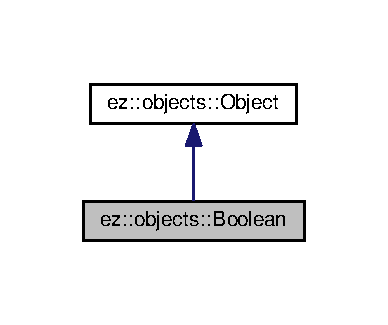
\includegraphics[width=186pt]{classez_1_1objects_1_1Boolean__inherit__graph}
\end{center}
\end{figure}


Collaboration diagram for ez\+:\+:objects\+:\+:Boolean\+:
\nopagebreak
\begin{figure}[H]
\begin{center}
\leavevmode
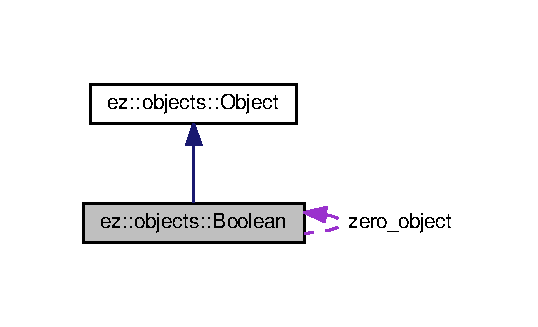
\includegraphics[width=258pt]{classez_1_1objects_1_1Boolean__coll__graph}
\end{center}
\end{figure}
\subsection*{Public Types}
\begin{DoxyCompactItemize}
\item 
\mbox{\Hypertarget{classez_1_1objects_1_1Boolean_ac3651f6ce091b0d95d5dd3480731e355}\label{classez_1_1objects_1_1Boolean_ac3651f6ce091b0d95d5dd3480731e355}} 
typedef \hyperlink{classez_1_1objects_1_1Boolean}{Boolean} {\bfseries self}
\end{DoxyCompactItemize}
\subsection*{Public Member Functions}
\begin{DoxyCompactItemize}
\item 
\hyperlink{classez_1_1objects_1_1Boolean_a9eee9d7b6285d1d4aeb28e7b64fba3d1}{Boolean} ()
\item 
\hyperlink{classez_1_1objects_1_1Boolean_a38c5fa82d29626076a027b615ddc64b8}{Boolean} (boolean v)
\item 
\hyperlink{classez_1_1objects_1_1Boolean_a59cf0c39db6caa85a04e26e179523252}{Boolean} (const \hyperlink{classez_1_1objects_1_1Boolean}{self} \&obj)
\item 
\hyperlink{classez_1_1objects_1_1Boolean}{self} \& \hyperlink{classez_1_1objects_1_1Boolean_a4c112c8a5f7e35bd4de19f0b52fa74c7}{operator=} (const \hyperlink{classez_1_1objects_1_1Boolean}{self} \&obj)
\item 
\hyperlink{classez_1_1objects_1_1Boolean_a1650855ce9987132244eb04905f8585b}{$\sim$\+Boolean} ()
\item 
\mbox{\Hypertarget{classez_1_1objects_1_1Boolean_abf2cb11539f4e11e82c0b3d7fdf05f5c}\label{classez_1_1objects_1_1Boolean_abf2cb11539f4e11e82c0b3d7fdf05f5c}} 
bool {\bfseries value} ()
\item 
\mbox{\Hypertarget{classez_1_1objects_1_1Boolean_a2065875fcf73101f468c5023ba56ff96}\label{classez_1_1objects_1_1Boolean_a2065875fcf73101f468c5023ba56ff96}} 
void {\bfseries value} (bool b)
\item 
integer \hyperlink{classez_1_1objects_1_1Boolean_a6ccc996f98fece5fbe6fd6ebcbd39f4a}{compare} (const \hyperlink{classez_1_1objects_1_1Object}{Object} \&y)
\item 
void \hyperlink{classez_1_1objects_1_1Boolean_aeedca84417b36666eb237d8453b744b6}{print} (std\+::ostream \&stream)
\item 
void \hyperlink{classez_1_1objects_1_1Boolean_a313c385e8ce93e19fd774882143f3a25}{output} (std\+::ostream \&stream)
\item 
void \hyperlink{classez_1_1objects_1_1Boolean_a36f2ae3b2e092b0f6f1d4c0be108e9e3}{input} (std\+::istream \&stream)
\item 
\hyperlink{classez_1_1objects_1_1Object}{Object} $\ast$ \hyperlink{classez_1_1objects_1_1Boolean_a3b1b1775d4869ba005cf4d20623d1260}{clone} ()
\item 
\mbox{\Hypertarget{classez_1_1objects_1_1Boolean_a197f6db133b2196797226edd6bf1e4e0}\label{classez_1_1objects_1_1Boolean_a197f6db133b2196797226edd6bf1e4e0}} 
\hyperlink{classez_1_1objects_1_1Boolean}{self} {\bfseries operator-\/} ()
\item 
\mbox{\Hypertarget{classez_1_1objects_1_1Boolean_afcffd74fa28f53e2668ca7b7a1a862df}\label{classez_1_1objects_1_1Boolean_afcffd74fa28f53e2668ca7b7a1a862df}} 
\hyperlink{classez_1_1objects_1_1Boolean}{self} {\bfseries operator$\sim$} ()
\item 
\mbox{\Hypertarget{classez_1_1objects_1_1Boolean_a22ce5ecbc0b5bd2109d415f240db9b05}\label{classez_1_1objects_1_1Boolean_a22ce5ecbc0b5bd2109d415f240db9b05}} 
\hyperlink{classez_1_1objects_1_1Boolean}{self} \& {\bfseries operator+=} (const \hyperlink{classez_1_1objects_1_1Boolean}{self} \&y)
\item 
\mbox{\Hypertarget{classez_1_1objects_1_1Boolean_a474e9cf9c243edca2e8a801163626ec1}\label{classez_1_1objects_1_1Boolean_a474e9cf9c243edca2e8a801163626ec1}} 
\hyperlink{classez_1_1objects_1_1Boolean}{self} \& {\bfseries operator$\ast$=} (const \hyperlink{classez_1_1objects_1_1Boolean}{self} \&y)
\item 
\mbox{\Hypertarget{classez_1_1objects_1_1Boolean_a6a5ec24705da1c4094397e7b76d34744}\label{classez_1_1objects_1_1Boolean_a6a5ec24705da1c4094397e7b76d34744}} 
bool {\bfseries min} ()
\item 
\mbox{\Hypertarget{classez_1_1objects_1_1Boolean_ad118af05489aa8cc511b1dc8d39f4257}\label{classez_1_1objects_1_1Boolean_ad118af05489aa8cc511b1dc8d39f4257}} 
bool {\bfseries max} ()
\end{DoxyCompactItemize}
\subsection*{Data Fields}
\begin{DoxyCompactItemize}
\item 
boolean \hyperlink{classez_1_1objects_1_1Boolean_a535d669406c4dae958e2ce00b2a339d3}{m\+\_\+value}
\end{DoxyCompactItemize}
\subsection*{Static Public Attributes}
\begin{DoxyCompactItemize}
\item 
static boolean \hyperlink{classez_1_1objects_1_1Boolean_aeb78b2275c789e764ceebe3bb7e86945}{zero} = false
\item 
static \hyperlink{classez_1_1objects_1_1Boolean}{Boolean} \hyperlink{classez_1_1objects_1_1Boolean_ab42b94b5b5ddc33cd64501447fdaa33c}{zero\+\_\+object}
\end{DoxyCompactItemize}
\subsection*{Friends}
\begin{DoxyCompactItemize}
\item 
\mbox{\Hypertarget{classez_1_1objects_1_1Boolean_a7b359bdb7de734892f01f402d9aaeb54}\label{classez_1_1objects_1_1Boolean_a7b359bdb7de734892f01f402d9aaeb54}} 
\hyperlink{classez_1_1objects_1_1Boolean}{self} {\bfseries operator \&} (const \hyperlink{classez_1_1objects_1_1Boolean}{self} \&x, const \hyperlink{classez_1_1objects_1_1Boolean}{self} \&y)
\item 
\mbox{\Hypertarget{classez_1_1objects_1_1Boolean_a1f142e40dd9c5d7d535c06ea59cc62ff}\label{classez_1_1objects_1_1Boolean_a1f142e40dd9c5d7d535c06ea59cc62ff}} 
\hyperlink{classez_1_1objects_1_1Boolean}{self} {\bfseries operator$\vert$} (const \hyperlink{classez_1_1objects_1_1Boolean}{self} \&x, const \hyperlink{classez_1_1objects_1_1Boolean}{self} \&y)
\item 
\mbox{\Hypertarget{classez_1_1objects_1_1Boolean_af2fec163038c670c3c6c48f08fc546ab}\label{classez_1_1objects_1_1Boolean_af2fec163038c670c3c6c48f08fc546ab}} 
\hyperlink{classez_1_1objects_1_1Boolean}{self} {\bfseries operator$^\wedge$} (const \hyperlink{classez_1_1objects_1_1Boolean}{self} \&x, const \hyperlink{classez_1_1objects_1_1Boolean}{self} \&y)
\item 
\mbox{\Hypertarget{classez_1_1objects_1_1Boolean_ac219ecb06730e7707b9bb78b5da63c3b}\label{classez_1_1objects_1_1Boolean_ac219ecb06730e7707b9bb78b5da63c3b}} 
\hyperlink{classez_1_1objects_1_1Boolean}{self} {\bfseries operator+} (const \hyperlink{classez_1_1objects_1_1Boolean}{self} x, const \hyperlink{classez_1_1objects_1_1Boolean}{self} y)
\item 
\mbox{\Hypertarget{classez_1_1objects_1_1Boolean_a4f9af882c7a074ed8e1f8da41bd31dc9}\label{classez_1_1objects_1_1Boolean_a4f9af882c7a074ed8e1f8da41bd31dc9}} 
\hyperlink{classez_1_1objects_1_1Boolean}{self} {\bfseries operator$\ast$} (const \hyperlink{classez_1_1objects_1_1Boolean}{self} x, const \hyperlink{classez_1_1objects_1_1Boolean}{self} y)
\end{DoxyCompactItemize}
\subsection*{Additional Inherited Members}


\subsection{Constructor \& Destructor Documentation}
\mbox{\Hypertarget{classez_1_1objects_1_1Boolean_a9eee9d7b6285d1d4aeb28e7b64fba3d1}\label{classez_1_1objects_1_1Boolean_a9eee9d7b6285d1d4aeb28e7b64fba3d1}} 
\index{ez\+::objects\+::\+Boolean@{ez\+::objects\+::\+Boolean}!Boolean@{Boolean}}
\index{Boolean@{Boolean}!ez\+::objects\+::\+Boolean@{ez\+::objects\+::\+Boolean}}
\subsubsection{\texorpdfstring{Boolean()}{Boolean()}\hspace{0.1cm}{\footnotesize\ttfamily [1/3]}}
{\footnotesize\ttfamily ez\+::objects\+::\+Boolean\+::\+Boolean (\begin{DoxyParamCaption}{ }\end{DoxyParamCaption})\hspace{0.3cm}{\ttfamily [inline]}}

default constructor \mbox{\Hypertarget{classez_1_1objects_1_1Boolean_a38c5fa82d29626076a027b615ddc64b8}\label{classez_1_1objects_1_1Boolean_a38c5fa82d29626076a027b615ddc64b8}} 
\index{ez\+::objects\+::\+Boolean@{ez\+::objects\+::\+Boolean}!Boolean@{Boolean}}
\index{Boolean@{Boolean}!ez\+::objects\+::\+Boolean@{ez\+::objects\+::\+Boolean}}
\subsubsection{\texorpdfstring{Boolean()}{Boolean()}\hspace{0.1cm}{\footnotesize\ttfamily [2/3]}}
{\footnotesize\ttfamily ez\+::objects\+::\+Boolean\+::\+Boolean (\begin{DoxyParamCaption}\item[{boolean}]{v }\end{DoxyParamCaption})\hspace{0.3cm}{\ttfamily [inline]}}

constructor given a value 
\begin{DoxyParams}{Parameters}
{\em v} & boolean value \\
\hline
\end{DoxyParams}
\mbox{\Hypertarget{classez_1_1objects_1_1Boolean_a59cf0c39db6caa85a04e26e179523252}\label{classez_1_1objects_1_1Boolean_a59cf0c39db6caa85a04e26e179523252}} 
\index{ez\+::objects\+::\+Boolean@{ez\+::objects\+::\+Boolean}!Boolean@{Boolean}}
\index{Boolean@{Boolean}!ez\+::objects\+::\+Boolean@{ez\+::objects\+::\+Boolean}}
\subsubsection{\texorpdfstring{Boolean()}{Boolean()}\hspace{0.1cm}{\footnotesize\ttfamily [3/3]}}
{\footnotesize\ttfamily ez\+::objects\+::\+Boolean\+::\+Boolean (\begin{DoxyParamCaption}\item[{const \hyperlink{classez_1_1objects_1_1Boolean}{self} \&}]{obj }\end{DoxyParamCaption})\hspace{0.3cm}{\ttfamily [inline]}}

copy constructor 
\begin{DoxyParams}{Parameters}
{\em obj} & reference to existing object \\
\hline
\end{DoxyParams}
\mbox{\Hypertarget{classez_1_1objects_1_1Boolean_a1650855ce9987132244eb04905f8585b}\label{classez_1_1objects_1_1Boolean_a1650855ce9987132244eb04905f8585b}} 
\index{ez\+::objects\+::\+Boolean@{ez\+::objects\+::\+Boolean}!````~Boolean@{$\sim$\+Boolean}}
\index{````~Boolean@{$\sim$\+Boolean}!ez\+::objects\+::\+Boolean@{ez\+::objects\+::\+Boolean}}
\subsubsection{\texorpdfstring{$\sim$\+Boolean()}{~Boolean()}}
{\footnotesize\ttfamily ez\+::objects\+::\+Boolean\+::$\sim$\+Boolean (\begin{DoxyParamCaption}{ }\end{DoxyParamCaption})\hspace{0.3cm}{\ttfamily [inline]}}

destructor 

\subsection{Member Function Documentation}
\mbox{\Hypertarget{classez_1_1objects_1_1Boolean_a3b1b1775d4869ba005cf4d20623d1260}\label{classez_1_1objects_1_1Boolean_a3b1b1775d4869ba005cf4d20623d1260}} 
\index{ez\+::objects\+::\+Boolean@{ez\+::objects\+::\+Boolean}!clone@{clone}}
\index{clone@{clone}!ez\+::objects\+::\+Boolean@{ez\+::objects\+::\+Boolean}}
\subsubsection{\texorpdfstring{clone()}{clone()}}
{\footnotesize\ttfamily \hyperlink{classez_1_1objects_1_1Object}{Object}$\ast$ ez\+::objects\+::\+Boolean\+::clone (\begin{DoxyParamCaption}{ }\end{DoxyParamCaption})\hspace{0.3cm}{\ttfamily [inline]}, {\ttfamily [virtual]}}

return a copy of the object 

Reimplemented from \hyperlink{classez_1_1objects_1_1Object_acf444b2581d898eb4b8c92c2d5865c9e}{ez\+::objects\+::\+Object}.

\mbox{\Hypertarget{classez_1_1objects_1_1Boolean_a6ccc996f98fece5fbe6fd6ebcbd39f4a}\label{classez_1_1objects_1_1Boolean_a6ccc996f98fece5fbe6fd6ebcbd39f4a}} 
\index{ez\+::objects\+::\+Boolean@{ez\+::objects\+::\+Boolean}!compare@{compare}}
\index{compare@{compare}!ez\+::objects\+::\+Boolean@{ez\+::objects\+::\+Boolean}}
\subsubsection{\texorpdfstring{compare()}{compare()}}
{\footnotesize\ttfamily integer ez\+::objects\+::\+Boolean\+::compare (\begin{DoxyParamCaption}\item[{const \hyperlink{classez_1_1objects_1_1Object}{Object} \&}]{y }\end{DoxyParamCaption})\hspace{0.3cm}{\ttfamily [inline]}, {\ttfamily [virtual]}}

redefinition of compare function for integers (\begin{DoxySeeAlso}{See also}
\hyperlink{classez_1_1objects_1_1Object}{Object}) 
\end{DoxySeeAlso}

\begin{DoxyParams}{Parameters}
{\em x} & must be a \hyperlink{classez_1_1objects_1_1Boolean}{Boolean} object \\
\hline
{\em y} & must be a \hyperlink{classez_1_1objects_1_1Boolean}{Boolean} object \\
\hline
\end{DoxyParams}
\begin{DoxyReturn}{Returns}
0 if both object have same value, a value less than zero if x=false and y=true, a value greater than 0 otherwise 
\end{DoxyReturn}


Reimplemented from \hyperlink{classez_1_1objects_1_1Object_aca311d389dffa204e425463145f4e1e6}{ez\+::objects\+::\+Object}.

\mbox{\Hypertarget{classez_1_1objects_1_1Boolean_a36f2ae3b2e092b0f6f1d4c0be108e9e3}\label{classez_1_1objects_1_1Boolean_a36f2ae3b2e092b0f6f1d4c0be108e9e3}} 
\index{ez\+::objects\+::\+Boolean@{ez\+::objects\+::\+Boolean}!input@{input}}
\index{input@{input}!ez\+::objects\+::\+Boolean@{ez\+::objects\+::\+Boolean}}
\subsubsection{\texorpdfstring{input()}{input()}}
{\footnotesize\ttfamily void Boolean\+::input (\begin{DoxyParamCaption}\item[{std\+::istream \&}]{stream }\end{DoxyParamCaption})\hspace{0.3cm}{\ttfamily [virtual]}}

overloading of input method 

Reimplemented from \hyperlink{classez_1_1objects_1_1Object_a878bdc53b7f16fda6fa15dab214c4b6a}{ez\+::objects\+::\+Object}.

\mbox{\Hypertarget{classez_1_1objects_1_1Boolean_a4c112c8a5f7e35bd4de19f0b52fa74c7}\label{classez_1_1objects_1_1Boolean_a4c112c8a5f7e35bd4de19f0b52fa74c7}} 
\index{ez\+::objects\+::\+Boolean@{ez\+::objects\+::\+Boolean}!operator=@{operator=}}
\index{operator=@{operator=}!ez\+::objects\+::\+Boolean@{ez\+::objects\+::\+Boolean}}
\subsubsection{\texorpdfstring{operator=()}{operator=()}}
{\footnotesize\ttfamily \hyperlink{classez_1_1objects_1_1Boolean}{self}\& ez\+::objects\+::\+Boolean\+::operator= (\begin{DoxyParamCaption}\item[{const \hyperlink{classez_1_1objects_1_1Boolean}{self} \&}]{obj }\end{DoxyParamCaption})\hspace{0.3cm}{\ttfamily [inline]}}

assignment operator 
\begin{DoxyParams}{Parameters}
{\em obj} & reference to existing object \\
\hline
\end{DoxyParams}
\begin{DoxyReturn}{Returns}
reference to this object 
\end{DoxyReturn}
\mbox{\Hypertarget{classez_1_1objects_1_1Boolean_a313c385e8ce93e19fd774882143f3a25}\label{classez_1_1objects_1_1Boolean_a313c385e8ce93e19fd774882143f3a25}} 
\index{ez\+::objects\+::\+Boolean@{ez\+::objects\+::\+Boolean}!output@{output}}
\index{output@{output}!ez\+::objects\+::\+Boolean@{ez\+::objects\+::\+Boolean}}
\subsubsection{\texorpdfstring{output()}{output()}}
{\footnotesize\ttfamily void Boolean\+::output (\begin{DoxyParamCaption}\item[{std\+::ostream \&}]{stream }\end{DoxyParamCaption})\hspace{0.3cm}{\ttfamily [virtual]}}

overloading of output method 

Reimplemented from \hyperlink{classez_1_1objects_1_1Object_a0fdfe18e6c35d6b0d7e7a01265aded15}{ez\+::objects\+::\+Object}.

\mbox{\Hypertarget{classez_1_1objects_1_1Boolean_aeedca84417b36666eb237d8453b744b6}\label{classez_1_1objects_1_1Boolean_aeedca84417b36666eb237d8453b744b6}} 
\index{ez\+::objects\+::\+Boolean@{ez\+::objects\+::\+Boolean}!print@{print}}
\index{print@{print}!ez\+::objects\+::\+Boolean@{ez\+::objects\+::\+Boolean}}
\subsubsection{\texorpdfstring{print()}{print()}}
{\footnotesize\ttfamily void Boolean\+::print (\begin{DoxyParamCaption}\item[{std\+::ostream \&}]{stream }\end{DoxyParamCaption})\hspace{0.3cm}{\ttfamily [virtual]}}

overloading of print method 

Reimplemented from \hyperlink{classez_1_1objects_1_1Object_a9e20f39a78163f67f000576149d858b3}{ez\+::objects\+::\+Object}.



\subsection{Field Documentation}
\mbox{\Hypertarget{classez_1_1objects_1_1Boolean_a535d669406c4dae958e2ce00b2a339d3}\label{classez_1_1objects_1_1Boolean_a535d669406c4dae958e2ce00b2a339d3}} 
\index{ez\+::objects\+::\+Boolean@{ez\+::objects\+::\+Boolean}!m\+\_\+value@{m\+\_\+value}}
\index{m\+\_\+value@{m\+\_\+value}!ez\+::objects\+::\+Boolean@{ez\+::objects\+::\+Boolean}}
\subsubsection{\texorpdfstring{m\+\_\+value}{m\_value}}
{\footnotesize\ttfamily boolean ez\+::objects\+::\+Boolean\+::m\+\_\+value}

value stored by this object \mbox{\Hypertarget{classez_1_1objects_1_1Boolean_aeb78b2275c789e764ceebe3bb7e86945}\label{classez_1_1objects_1_1Boolean_aeb78b2275c789e764ceebe3bb7e86945}} 
\index{ez\+::objects\+::\+Boolean@{ez\+::objects\+::\+Boolean}!zero@{zero}}
\index{zero@{zero}!ez\+::objects\+::\+Boolean@{ez\+::objects\+::\+Boolean}}
\subsubsection{\texorpdfstring{zero}{zero}}
{\footnotesize\ttfamily boolean Boolean\+::zero = false\hspace{0.3cm}{\ttfamily [static]}}

definition of zero for the boolean type \mbox{\Hypertarget{classez_1_1objects_1_1Boolean_ab42b94b5b5ddc33cd64501447fdaa33c}\label{classez_1_1objects_1_1Boolean_ab42b94b5b5ddc33cd64501447fdaa33c}} 
\index{ez\+::objects\+::\+Boolean@{ez\+::objects\+::\+Boolean}!zero\+\_\+object@{zero\+\_\+object}}
\index{zero\+\_\+object@{zero\+\_\+object}!ez\+::objects\+::\+Boolean@{ez\+::objects\+::\+Boolean}}
\subsubsection{\texorpdfstring{zero\+\_\+object}{zero\_object}}
{\footnotesize\ttfamily \hyperlink{classez_1_1objects_1_1Boolean}{Boolean} Boolean\+::zero\+\_\+object\hspace{0.3cm}{\ttfamily [static]}}

definition of object with zero value for the \hyperlink{classez_1_1objects_1_1Boolean}{Boolean} class 

The documentation for this class was generated from the following files\+:\begin{DoxyCompactItemize}
\item 
src/version\+\_\+2018.\+06/objects/boolean.\+h\item 
src/version\+\_\+2018.\+06/objects/boolean.\+cpp\end{DoxyCompactItemize}

\hypertarget{classez_1_1arguments_1_1BooleanArgument}{}\section{ez\+:\+:arguments\+:\+:Boolean\+Argument Class Reference}
\label{classez_1_1arguments_1_1BooleanArgument}\index{ez\+::arguments\+::\+Boolean\+Argument@{ez\+::arguments\+::\+Boolean\+Argument}}


{\ttfamily \#include $<$boolean\+\_\+argument.\+h$>$}



Inheritance diagram for ez\+:\+:arguments\+:\+:Boolean\+Argument\+:
\nopagebreak
\begin{figure}[H]
\begin{center}
\leavevmode
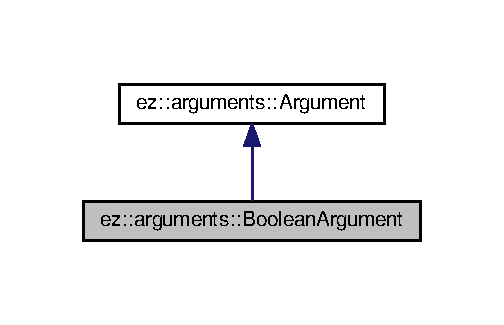
\includegraphics[width=242pt]{classez_1_1arguments_1_1BooleanArgument__inherit__graph}
\end{center}
\end{figure}


Collaboration diagram for ez\+:\+:arguments\+:\+:Boolean\+Argument\+:
\nopagebreak
\begin{figure}[H]
\begin{center}
\leavevmode
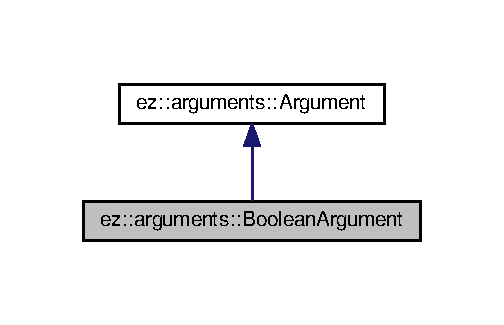
\includegraphics[width=242pt]{classez_1_1arguments_1_1BooleanArgument__coll__graph}
\end{center}
\end{figure}
\subsection*{Public Member Functions}
\begin{DoxyCompactItemize}
\item 
\hyperlink{classez_1_1arguments_1_1BooleanArgument_a1d5bfd420e261e25ce2d3efc175ee7b0}{Boolean\+Argument} (string long\+\_\+label, char short\+\_\+label, bool $\ast$value, string description, trigger\+\_\+t trigger=nullptr)
\item 
\mbox{\Hypertarget{classez_1_1arguments_1_1BooleanArgument_af242aa0103bac81883b6d5b5e6861ad7}\label{classez_1_1arguments_1_1BooleanArgument_af242aa0103bac81883b6d5b5e6861ad7}} 
void {\bfseries parse} (string \&s)
\end{DoxyCompactItemize}
\subsection*{Protected Attributes}
\begin{DoxyCompactItemize}
\item 
\mbox{\Hypertarget{classez_1_1arguments_1_1BooleanArgument_a4744f07800453f73d2305bcf92be1ef0}\label{classez_1_1arguments_1_1BooleanArgument_a4744f07800453f73d2305bcf92be1ef0}} 
bool $\ast$ {\bfseries m\+\_\+value}
\end{DoxyCompactItemize}


\subsection{Detailed Description}
class used to treat boolean argument 

\subsection{Constructor \& Destructor Documentation}
\mbox{\Hypertarget{classez_1_1arguments_1_1BooleanArgument_a1d5bfd420e261e25ce2d3efc175ee7b0}\label{classez_1_1arguments_1_1BooleanArgument_a1d5bfd420e261e25ce2d3efc175ee7b0}} 
\index{ez\+::arguments\+::\+Boolean\+Argument@{ez\+::arguments\+::\+Boolean\+Argument}!Boolean\+Argument@{Boolean\+Argument}}
\index{Boolean\+Argument@{Boolean\+Argument}!ez\+::arguments\+::\+Boolean\+Argument@{ez\+::arguments\+::\+Boolean\+Argument}}
\subsubsection{\texorpdfstring{Boolean\+Argument()}{BooleanArgument()}}
{\footnotesize\ttfamily ez\+::arguments\+::\+Boolean\+Argument\+::\+Boolean\+Argument (\begin{DoxyParamCaption}\item[{string}]{long\+\_\+label,  }\item[{char}]{short\+\_\+label,  }\item[{bool $\ast$}]{value,  }\item[{string}]{description,  }\item[{trigger\+\_\+t}]{trigger = {\ttfamily nullptr} }\end{DoxyParamCaption})\hspace{0.3cm}{\ttfamily [inline]}}

constructor with pointer to boolean value to set 

The documentation for this class was generated from the following files\+:\begin{DoxyCompactItemize}
\item 
src/version\+\_\+2018.\+06/arguments/boolean\+\_\+argument.\+h\item 
src/version\+\_\+2018.\+06/arguments/boolean\+\_\+argument.\+cpp\end{DoxyCompactItemize}

\hypertarget{classez_1_1maths_1_1BoundingBox3D}{}\section{ez\+:\+:maths\+:\+:Bounding\+Box3D Class Reference}
\label{classez_1_1maths_1_1BoundingBox3D}\index{ez\+::maths\+::\+Bounding\+Box3D@{ez\+::maths\+::\+Bounding\+Box3D}}


Collaboration diagram for ez\+:\+:maths\+:\+:Bounding\+Box3D\+:
\nopagebreak
\begin{figure}[H]
\begin{center}
\leavevmode
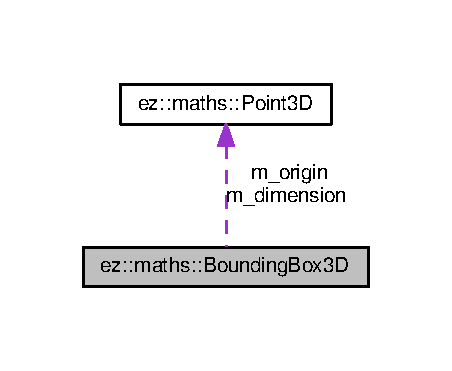
\includegraphics[width=217pt]{classez_1_1maths_1_1BoundingBox3D__coll__graph}
\end{center}
\end{figure}
\subsection*{Public Member Functions}
\begin{DoxyCompactItemize}
\item 
\hyperlink{classez_1_1maths_1_1BoundingBox3D_a81a912b95fbb8c30afd2550ef8b77f61}{Bounding\+Box3D} ()
\item 
\mbox{\Hypertarget{classez_1_1maths_1_1BoundingBox3D_a92da1569fe2f3d46a08876d1f627be25}\label{classez_1_1maths_1_1BoundingBox3D_a92da1569fe2f3d46a08876d1f627be25}} 
{\bfseries Bounding\+Box3D} (\hyperlink{classez_1_1maths_1_1Point3D}{Point3D} origin, \hyperlink{classez_1_1maths_1_1Point3D}{Point3D} dimension)
\item 
\mbox{\Hypertarget{classez_1_1maths_1_1BoundingBox3D_a65def50508834c47c7cd12feb5aaaaa2}\label{classez_1_1maths_1_1BoundingBox3D_a65def50508834c47c7cd12feb5aaaaa2}} 
\hyperlink{classez_1_1maths_1_1BoundingBox3D}{Bounding\+Box3D} \& {\bfseries operator=} (const \hyperlink{classez_1_1maths_1_1BoundingBox3D}{Bounding\+Box3D} \&obj)
\item 
\mbox{\Hypertarget{classez_1_1maths_1_1BoundingBox3D_abf08015dca3aeb42e8d0348b221885a4}\label{classez_1_1maths_1_1BoundingBox3D_abf08015dca3aeb42e8d0348b221885a4}} 
long\+\_\+real {\bfseries o\+\_\+x} ()
\item 
\mbox{\Hypertarget{classez_1_1maths_1_1BoundingBox3D_adaa6f2b45fb82aab1d513bf5c3380579}\label{classez_1_1maths_1_1BoundingBox3D_adaa6f2b45fb82aab1d513bf5c3380579}} 
long\+\_\+real {\bfseries o\+\_\+y} ()
\item 
\mbox{\Hypertarget{classez_1_1maths_1_1BoundingBox3D_a5a4364a3614aacaaf19169439ff0216b}\label{classez_1_1maths_1_1BoundingBox3D_a5a4364a3614aacaaf19169439ff0216b}} 
long\+\_\+real {\bfseries o\+\_\+z} ()
\item 
\mbox{\Hypertarget{classez_1_1maths_1_1BoundingBox3D_a07490c368d321b10191295310bda6605}\label{classez_1_1maths_1_1BoundingBox3D_a07490c368d321b10191295310bda6605}} 
long\+\_\+real {\bfseries d\+\_\+x} ()
\item 
\mbox{\Hypertarget{classez_1_1maths_1_1BoundingBox3D_a8169a716fbdfd8321dd0b11fe95c1635}\label{classez_1_1maths_1_1BoundingBox3D_a8169a716fbdfd8321dd0b11fe95c1635}} 
long\+\_\+real {\bfseries d\+\_\+y} ()
\item 
\mbox{\Hypertarget{classez_1_1maths_1_1BoundingBox3D_a82d4fae5feb0c8bb93dcb44ad5d38356}\label{classez_1_1maths_1_1BoundingBox3D_a82d4fae5feb0c8bb93dcb44ad5d38356}} 
long\+\_\+real {\bfseries d\+\_\+z} ()
\item 
bool \hyperlink{classez_1_1maths_1_1BoundingBox3D_ab69a5ee522212f8b8c0bf8ab7368620c}{is\+\_\+inside} (\hyperlink{classez_1_1maths_1_1Point3D}{Point3D} \&p)
\item 
\mbox{\Hypertarget{classez_1_1maths_1_1BoundingBox3D_aa22da905a92088ee3ef4772164b19a4d}\label{classez_1_1maths_1_1BoundingBox3D_aa22da905a92088ee3ef4772164b19a4d}} 
ostream \& {\bfseries print} (ostream \&out)
\end{DoxyCompactItemize}
\subsection*{Static Public Member Functions}
\begin{DoxyCompactItemize}
\item 
static void \hyperlink{classez_1_1maths_1_1BoundingBox3D_a64f9ec4f9a6f62e9d253526733f630d5}{compute\+\_\+box} (\hyperlink{classez_1_1objects_1_1Vector}{ez\+::objects\+::\+Vector}$<$ \hyperlink{classez_1_1maths_1_1Point3D}{Point3D} $>$ \&v, \hyperlink{classez_1_1maths_1_1BoundingBox3D}{Bounding\+Box3D} \&b)
\end{DoxyCompactItemize}
\subsection*{Data Fields}
\begin{DoxyCompactItemize}
\item 
\mbox{\Hypertarget{classez_1_1maths_1_1BoundingBox3D_ad93421fd16aa004ad0caf9ec9dae8f63}\label{classez_1_1maths_1_1BoundingBox3D_ad93421fd16aa004ad0caf9ec9dae8f63}} 
\hyperlink{classez_1_1maths_1_1Point3D}{Point3D} {\bfseries m\+\_\+origin}
\item 
\mbox{\Hypertarget{classez_1_1maths_1_1BoundingBox3D_ac237f04a44c7a380df70e585f71c958c}\label{classez_1_1maths_1_1BoundingBox3D_ac237f04a44c7a380df70e585f71c958c}} 
\hyperlink{classez_1_1maths_1_1Point3D}{Point3D} {\bfseries m\+\_\+dimension}
\end{DoxyCompactItemize}
\subsection*{Friends}
\begin{DoxyCompactItemize}
\item 
\mbox{\Hypertarget{classez_1_1maths_1_1BoundingBox3D_a82bf56a0187cec6d234de15d321c78b4}\label{classez_1_1maths_1_1BoundingBox3D_a82bf56a0187cec6d234de15d321c78b4}} 
ostream \& {\bfseries operator$<$$<$} (ostream \&out, \hyperlink{classez_1_1maths_1_1BoundingBox3D}{Bounding\+Box3D} \&obj)
\end{DoxyCompactItemize}


\subsection{Constructor \& Destructor Documentation}
\mbox{\Hypertarget{classez_1_1maths_1_1BoundingBox3D_a81a912b95fbb8c30afd2550ef8b77f61}\label{classez_1_1maths_1_1BoundingBox3D_a81a912b95fbb8c30afd2550ef8b77f61}} 
\index{ez\+::maths\+::\+Bounding\+Box3D@{ez\+::maths\+::\+Bounding\+Box3D}!Bounding\+Box3D@{Bounding\+Box3D}}
\index{Bounding\+Box3D@{Bounding\+Box3D}!ez\+::maths\+::\+Bounding\+Box3D@{ez\+::maths\+::\+Bounding\+Box3D}}
\subsubsection{\texorpdfstring{Bounding\+Box3\+D()}{BoundingBox3D()}}
{\footnotesize\ttfamily ez\+::maths\+::\+Bounding\+Box3\+D\+::\+Bounding\+Box3D (\begin{DoxyParamCaption}{ }\end{DoxyParamCaption})\hspace{0.3cm}{\ttfamily [inline]}}

Default constructor 

\subsection{Member Function Documentation}
\mbox{\Hypertarget{classez_1_1maths_1_1BoundingBox3D_a64f9ec4f9a6f62e9d253526733f630d5}\label{classez_1_1maths_1_1BoundingBox3D_a64f9ec4f9a6f62e9d253526733f630d5}} 
\index{ez\+::maths\+::\+Bounding\+Box3D@{ez\+::maths\+::\+Bounding\+Box3D}!compute\+\_\+box@{compute\+\_\+box}}
\index{compute\+\_\+box@{compute\+\_\+box}!ez\+::maths\+::\+Bounding\+Box3D@{ez\+::maths\+::\+Bounding\+Box3D}}
\subsubsection{\texorpdfstring{compute\+\_\+box()}{compute\_box()}}
{\footnotesize\ttfamily static void ez\+::maths\+::\+Bounding\+Box3\+D\+::compute\+\_\+box (\begin{DoxyParamCaption}\item[{\hyperlink{classez_1_1objects_1_1Vector}{ez\+::objects\+::\+Vector}$<$ \hyperlink{classez_1_1maths_1_1Point3D}{Point3D} $>$ \&}]{v,  }\item[{\hyperlink{classez_1_1maths_1_1BoundingBox3D}{Bounding\+Box3D} \&}]{b }\end{DoxyParamCaption})\hspace{0.3cm}{\ttfamily [static]}}

Find bounding box of a vector of \hyperlink{classez_1_1maths_1_1Point3D}{Point3D} 
\begin{DoxyParams}{Parameters}
{\em v} & \hyperlink{classez_1_1maths_1_1Vector}{Vector} of \hyperlink{classez_1_1maths_1_1Point3D}{Point3D} \\
\hline
{\em b} & bounding box that results from computation \\
\hline
\end{DoxyParams}
\mbox{\Hypertarget{classez_1_1maths_1_1BoundingBox3D_ab69a5ee522212f8b8c0bf8ab7368620c}\label{classez_1_1maths_1_1BoundingBox3D_ab69a5ee522212f8b8c0bf8ab7368620c}} 
\index{ez\+::maths\+::\+Bounding\+Box3D@{ez\+::maths\+::\+Bounding\+Box3D}!is\+\_\+inside@{is\+\_\+inside}}
\index{is\+\_\+inside@{is\+\_\+inside}!ez\+::maths\+::\+Bounding\+Box3D@{ez\+::maths\+::\+Bounding\+Box3D}}
\subsubsection{\texorpdfstring{is\+\_\+inside()}{is\_inside()}}
{\footnotesize\ttfamily bool Bounding\+Box3\+D\+::is\+\_\+inside (\begin{DoxyParamCaption}\item[{\hyperlink{classez_1_1maths_1_1Point3D}{Point3D} \&}]{p }\end{DoxyParamCaption})}

return true if point is inside box 

The documentation for this class was generated from the following files\+:\begin{DoxyCompactItemize}
\item 
src/version\+\_\+2018.\+06/maths/bounding\+\_\+box3d.\+h\item 
src/version\+\_\+2018.\+06/maths/bounding\+\_\+box3d.\+cpp\end{DoxyCompactItemize}

\hypertarget{classez_1_1objects_1_1Character}{}\section{ez\+:\+:objects\+:\+:Character Class Reference}
\label{classez_1_1objects_1_1Character}\index{ez\+::objects\+::\+Character@{ez\+::objects\+::\+Character}}


Inheritance diagram for ez\+:\+:objects\+:\+:Character\+:
\nopagebreak
\begin{figure}[H]
\begin{center}
\leavevmode
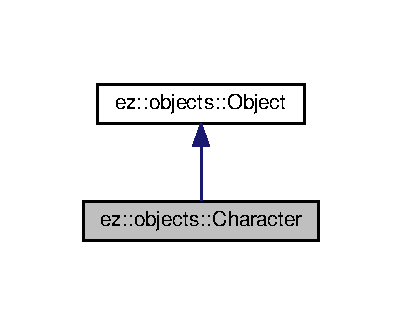
\includegraphics[width=193pt]{classez_1_1objects_1_1Character__inherit__graph}
\end{center}
\end{figure}


Collaboration diagram for ez\+:\+:objects\+:\+:Character\+:
\nopagebreak
\begin{figure}[H]
\begin{center}
\leavevmode
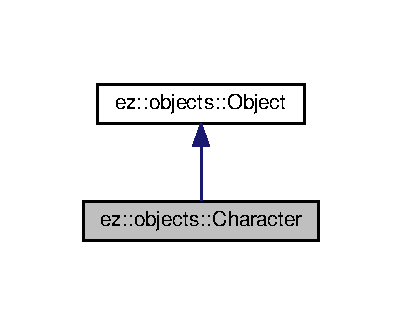
\includegraphics[width=193pt]{classez_1_1objects_1_1Character__coll__graph}
\end{center}
\end{figure}
\subsection*{Public Types}
\begin{DoxyCompactItemize}
\item 
\mbox{\Hypertarget{classez_1_1objects_1_1Character_a873c6f939973433df51a33b85daa95b5}\label{classez_1_1objects_1_1Character_a873c6f939973433df51a33b85daa95b5}} 
typedef \hyperlink{classez_1_1objects_1_1Character}{Character} {\bfseries self}
\end{DoxyCompactItemize}
\subsection*{Public Member Functions}
\begin{DoxyCompactItemize}
\item 
\mbox{\Hypertarget{classez_1_1objects_1_1Character_a6c31ce83af70a52bc13a082fb52bebb5}\label{classez_1_1objects_1_1Character_a6c31ce83af70a52bc13a082fb52bebb5}} 
{\bfseries Character} (character c)
\item 
\mbox{\Hypertarget{classez_1_1objects_1_1Character_aeed1a671762a384be0feec2df2e7ba22}\label{classez_1_1objects_1_1Character_aeed1a671762a384be0feec2df2e7ba22}} 
{\bfseries Character} (const \hyperlink{classez_1_1objects_1_1Character}{Character} \&object)
\item 
\mbox{\Hypertarget{classez_1_1objects_1_1Character_abbf053f6036426e1fd2f1f1ab2a2e8e5}\label{classez_1_1objects_1_1Character_abbf053f6036426e1fd2f1f1ab2a2e8e5}} 
\hyperlink{classez_1_1objects_1_1Character}{self} \& {\bfseries operator=} (const \hyperlink{classez_1_1objects_1_1Character}{self} \&object)
\item 
\mbox{\Hypertarget{classez_1_1objects_1_1Character_a73e6dc5e0dd21806829921636788b53c}\label{classez_1_1objects_1_1Character_a73e6dc5e0dd21806829921636788b53c}} 
character {\bfseries value} ()
\item 
\mbox{\Hypertarget{classez_1_1objects_1_1Character_a2e3430a7fada6e65312896e78c961c4b}\label{classez_1_1objects_1_1Character_a2e3430a7fada6e65312896e78c961c4b}} 
void {\bfseries value} (character c)
\item 
integer \hyperlink{classez_1_1objects_1_1Character_a2e6241f13a2f749e7b1951667b4ec96a}{compare} (const \hyperlink{classez_1_1objects_1_1Object}{Object} \&y)
\item 
void \hyperlink{classez_1_1objects_1_1Character_abf2e9f190594d03005b1cd0610f2f38c}{print} (std\+::ostream \&stream)
\item 
void \hyperlink{classez_1_1objects_1_1Character_ab72c114740fab4824d691d6219e07a67}{output} (std\+::ostream \&stream)
\item 
void \hyperlink{classez_1_1objects_1_1Character_a021f11fd444493316c4d55e6efb031f5}{input} (std\+::istream \&stream)
\item 
\hyperlink{classez_1_1objects_1_1Object}{Object} $\ast$ \hyperlink{classez_1_1objects_1_1Character_ad272c9b94a2d152f0832f2957cfd4e63}{clone} ()
\item 
bool \hyperlink{classez_1_1objects_1_1Character_ae94793b98d9c5a173ba73e110420f187}{is\+\_\+numeric} ()
\item 
\mbox{\Hypertarget{classez_1_1objects_1_1Character_a34411a36a4631183fa6022dfaca1c599}\label{classez_1_1objects_1_1Character_a34411a36a4631183fa6022dfaca1c599}} 
character {\bfseries min} ()
\item 
\mbox{\Hypertarget{classez_1_1objects_1_1Character_a82f9484062c83e4ef71411743d2c8b63}\label{classez_1_1objects_1_1Character_a82f9484062c83e4ef71411743d2c8b63}} 
character {\bfseries max} ()
\end{DoxyCompactItemize}
\subsection*{Data Fields}
\begin{DoxyCompactItemize}
\item 
\mbox{\Hypertarget{classez_1_1objects_1_1Character_aab5b89b7d8aac7509c9d23b4152cdb54}\label{classez_1_1objects_1_1Character_aab5b89b7d8aac7509c9d23b4152cdb54}} 
character {\bfseries m\+\_\+value}
\end{DoxyCompactItemize}
\subsection*{Additional Inherited Members}


\subsection{Member Function Documentation}
\mbox{\Hypertarget{classez_1_1objects_1_1Character_ad272c9b94a2d152f0832f2957cfd4e63}\label{classez_1_1objects_1_1Character_ad272c9b94a2d152f0832f2957cfd4e63}} 
\index{ez\+::objects\+::\+Character@{ez\+::objects\+::\+Character}!clone@{clone}}
\index{clone@{clone}!ez\+::objects\+::\+Character@{ez\+::objects\+::\+Character}}
\subsubsection{\texorpdfstring{clone()}{clone()}}
{\footnotesize\ttfamily \hyperlink{classez_1_1objects_1_1Object}{Object}$\ast$ ez\+::objects\+::\+Character\+::clone (\begin{DoxyParamCaption}{ }\end{DoxyParamCaption})\hspace{0.3cm}{\ttfamily [inline]}, {\ttfamily [virtual]}}

return a copy of the object 

Reimplemented from \hyperlink{classez_1_1objects_1_1Object_acf444b2581d898eb4b8c92c2d5865c9e}{ez\+::objects\+::\+Object}.

\mbox{\Hypertarget{classez_1_1objects_1_1Character_a2e6241f13a2f749e7b1951667b4ec96a}\label{classez_1_1objects_1_1Character_a2e6241f13a2f749e7b1951667b4ec96a}} 
\index{ez\+::objects\+::\+Character@{ez\+::objects\+::\+Character}!compare@{compare}}
\index{compare@{compare}!ez\+::objects\+::\+Character@{ez\+::objects\+::\+Character}}
\subsubsection{\texorpdfstring{compare()}{compare()}}
{\footnotesize\ttfamily integer ez\+::objects\+::\+Character\+::compare (\begin{DoxyParamCaption}\item[{const \hyperlink{classez_1_1objects_1_1Object}{Object} \&}]{y }\end{DoxyParamCaption})\hspace{0.3cm}{\ttfamily [inline]}, {\ttfamily [virtual]}}

redefinition of compare function for integers (\begin{DoxySeeAlso}{See also}
\hyperlink{classez_1_1objects_1_1Object}{Object}) 
\end{DoxySeeAlso}

\begin{DoxyParams}{Parameters}
{\em x} & must be a \hyperlink{classez_1_1objects_1_1Boolean}{Boolean} object \\
\hline
{\em y} & must be a \hyperlink{classez_1_1objects_1_1Boolean}{Boolean} object \\
\hline
\end{DoxyParams}
\begin{DoxyReturn}{Returns}
0 if both object have same value, a value less than zero if x=false and y=true, a value greater than 0 otherwise 
\end{DoxyReturn}


Reimplemented from \hyperlink{classez_1_1objects_1_1Object_aca311d389dffa204e425463145f4e1e6}{ez\+::objects\+::\+Object}.

\mbox{\Hypertarget{classez_1_1objects_1_1Character_a021f11fd444493316c4d55e6efb031f5}\label{classez_1_1objects_1_1Character_a021f11fd444493316c4d55e6efb031f5}} 
\index{ez\+::objects\+::\+Character@{ez\+::objects\+::\+Character}!input@{input}}
\index{input@{input}!ez\+::objects\+::\+Character@{ez\+::objects\+::\+Character}}
\subsubsection{\texorpdfstring{input()}{input()}}
{\footnotesize\ttfamily void Character\+::input (\begin{DoxyParamCaption}\item[{std\+::istream \&}]{stream }\end{DoxyParamCaption})\hspace{0.3cm}{\ttfamily [virtual]}}

this function is used to get the data field members of an object from a stream and acts as unserialize 

Reimplemented from \hyperlink{classez_1_1objects_1_1Object_a878bdc53b7f16fda6fa15dab214c4b6a}{ez\+::objects\+::\+Object}.

\mbox{\Hypertarget{classez_1_1objects_1_1Character_ae94793b98d9c5a173ba73e110420f187}\label{classez_1_1objects_1_1Character_ae94793b98d9c5a173ba73e110420f187}} 
\index{ez\+::objects\+::\+Character@{ez\+::objects\+::\+Character}!is\+\_\+numeric@{is\+\_\+numeric}}
\index{is\+\_\+numeric@{is\+\_\+numeric}!ez\+::objects\+::\+Character@{ez\+::objects\+::\+Character}}
\subsubsection{\texorpdfstring{is\+\_\+numeric()}{is\_numeric()}}
{\footnotesize\ttfamily bool ez\+::objects\+::\+Character\+::is\+\_\+numeric (\begin{DoxyParamCaption}{ }\end{DoxyParamCaption})\hspace{0.3cm}{\ttfamily [inline]}, {\ttfamily [virtual]}}

indicates if this object can be used for computation 

Reimplemented from \hyperlink{classez_1_1objects_1_1Object_a19ba1672d4063232c4619e016ca178f8}{ez\+::objects\+::\+Object}.

\mbox{\Hypertarget{classez_1_1objects_1_1Character_ab72c114740fab4824d691d6219e07a67}\label{classez_1_1objects_1_1Character_ab72c114740fab4824d691d6219e07a67}} 
\index{ez\+::objects\+::\+Character@{ez\+::objects\+::\+Character}!output@{output}}
\index{output@{output}!ez\+::objects\+::\+Character@{ez\+::objects\+::\+Character}}
\subsubsection{\texorpdfstring{output()}{output()}}
{\footnotesize\ttfamily void Character\+::output (\begin{DoxyParamCaption}\item[{std\+::ostream \&}]{stream }\end{DoxyParamCaption})\hspace{0.3cm}{\ttfamily [virtual]}}

this function is used to print the contents of the object in a serializable manner 

Reimplemented from \hyperlink{classez_1_1objects_1_1Object_a0fdfe18e6c35d6b0d7e7a01265aded15}{ez\+::objects\+::\+Object}.

\mbox{\Hypertarget{classez_1_1objects_1_1Character_abf2e9f190594d03005b1cd0610f2f38c}\label{classez_1_1objects_1_1Character_abf2e9f190594d03005b1cd0610f2f38c}} 
\index{ez\+::objects\+::\+Character@{ez\+::objects\+::\+Character}!print@{print}}
\index{print@{print}!ez\+::objects\+::\+Character@{ez\+::objects\+::\+Character}}
\subsubsection{\texorpdfstring{print()}{print()}}
{\footnotesize\ttfamily void Character\+::print (\begin{DoxyParamCaption}\item[{std\+::ostream \&}]{stream }\end{DoxyParamCaption})\hspace{0.3cm}{\ttfamily [virtual]}}

this function is used to print the contents of the object in a human readable format 
\begin{DoxyParams}{Parameters}
{\em stream} & output stream for example std\+::cout \\
\hline
\end{DoxyParams}


Reimplemented from \hyperlink{classez_1_1objects_1_1Object_a9e20f39a78163f67f000576149d858b3}{ez\+::objects\+::\+Object}.



The documentation for this class was generated from the following files\+:\begin{DoxyCompactItemize}
\item 
src/version\+\_\+2018.\+06/objects/character.\+h\item 
src/version\+\_\+2018.\+06/objects/character.\+cpp\end{DoxyCompactItemize}

\hypertarget{classez_1_1logging_1_1ConsoleLogger}{}\section{ez\+:\+:logging\+:\+:Console\+Logger Class Reference}
\label{classez_1_1logging_1_1ConsoleLogger}\index{ez\+::logging\+::\+Console\+Logger@{ez\+::logging\+::\+Console\+Logger}}


{\ttfamily \#include $<$logger.\+h$>$}



Inheritance diagram for ez\+:\+:logging\+:\+:Console\+Logger\+:
\nopagebreak
\begin{figure}[H]
\begin{center}
\leavevmode
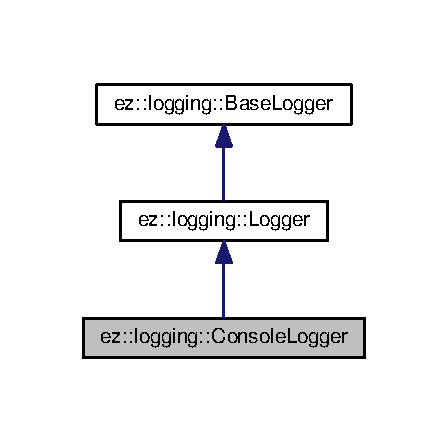
\includegraphics[width=215pt]{classez_1_1logging_1_1ConsoleLogger__inherit__graph}
\end{center}
\end{figure}


Collaboration diagram for ez\+:\+:logging\+:\+:Console\+Logger\+:
\nopagebreak
\begin{figure}[H]
\begin{center}
\leavevmode
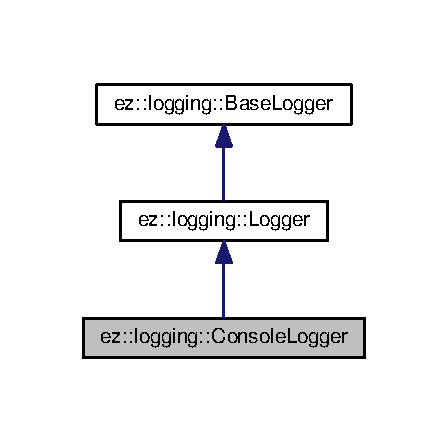
\includegraphics[width=215pt]{classez_1_1logging_1_1ConsoleLogger__coll__graph}
\end{center}
\end{figure}
\subsection*{Public Member Functions}
\begin{DoxyCompactItemize}
\item 
\hyperlink{classez_1_1logging_1_1ConsoleLogger_a6b9357ce75b0207d0cb68866584b0080}{Console\+Logger} (std\+::string name, std\+::ostream $\ast$out=\&std\+::cerr)
\item 
\hyperlink{classez_1_1logging_1_1ConsoleLogger_a242e88aa9495249d5a7fbdfc4f8886ee}{$\sim$\+Console\+Logger} ()
\item 
\mbox{\Hypertarget{classez_1_1logging_1_1ConsoleLogger_a66ac6d21ed4ee2657b79429b78bd16d2}\label{classez_1_1logging_1_1ConsoleLogger_a66ac6d21ed4ee2657b79429b78bd16d2}} 
\hyperlink{classez_1_1logging_1_1ConsoleLogger}{Console\+Logger} \& {\bfseries operator$<$$<$} (std\+::string \&s)
\end{DoxyCompactItemize}
\subsection*{Additional Inherited Members}


\subsection{Detailed Description}
\hyperlink{classez_1_1logging_1_1Logger}{Logger} that displays information on stdout or stderr 

\subsection{Constructor \& Destructor Documentation}
\mbox{\Hypertarget{classez_1_1logging_1_1ConsoleLogger_a6b9357ce75b0207d0cb68866584b0080}\label{classez_1_1logging_1_1ConsoleLogger_a6b9357ce75b0207d0cb68866584b0080}} 
\index{ez\+::logging\+::\+Console\+Logger@{ez\+::logging\+::\+Console\+Logger}!Console\+Logger@{Console\+Logger}}
\index{Console\+Logger@{Console\+Logger}!ez\+::logging\+::\+Console\+Logger@{ez\+::logging\+::\+Console\+Logger}}
\subsubsection{\texorpdfstring{Console\+Logger()}{ConsoleLogger()}}
{\footnotesize\ttfamily Console\+Logger\+::\+Console\+Logger (\begin{DoxyParamCaption}\item[{std\+::string}]{name,  }\item[{std\+::ostream $\ast$}]{out = {\ttfamily \&std\+:\+:cerr} }\end{DoxyParamCaption})}

constructor 
\begin{DoxyParams}{Parameters}
{\em name} & identifier of the logger \\
\hline
{\em out} & output stream \\
\hline
\end{DoxyParams}
\mbox{\Hypertarget{classez_1_1logging_1_1ConsoleLogger_a242e88aa9495249d5a7fbdfc4f8886ee}\label{classez_1_1logging_1_1ConsoleLogger_a242e88aa9495249d5a7fbdfc4f8886ee}} 
\index{ez\+::logging\+::\+Console\+Logger@{ez\+::logging\+::\+Console\+Logger}!````~Console\+Logger@{$\sim$\+Console\+Logger}}
\index{````~Console\+Logger@{$\sim$\+Console\+Logger}!ez\+::logging\+::\+Console\+Logger@{ez\+::logging\+::\+Console\+Logger}}
\subsubsection{\texorpdfstring{$\sim$\+Console\+Logger()}{~ConsoleLogger()}}
{\footnotesize\ttfamily Console\+Logger\+::$\sim$\+Console\+Logger (\begin{DoxyParamCaption}{ }\end{DoxyParamCaption})}

destructor 

The documentation for this class was generated from the following files\+:\begin{DoxyCompactItemize}
\item 
src/version\+\_\+2018.\+06/logging/logger.\+h\item 
src/version\+\_\+2018.\+06/logging/logger.\+cpp\end{DoxyCompactItemize}

\hypertarget{classez_1_1maths_1_1Constants}{}\section{ez\+:\+:maths\+:\+:Constants Class Reference}
\label{classez_1_1maths_1_1Constants}\index{ez\+::maths\+::\+Constants@{ez\+::maths\+::\+Constants}}
\subsection*{Static Public Attributes}
\begin{DoxyCompactItemize}
\item 
\mbox{\Hypertarget{classez_1_1maths_1_1Constants_a0561f868c8aafb751ac1264ed8f0dc5d}\label{classez_1_1maths_1_1Constants_a0561f868c8aafb751ac1264ed8f0dc5d}} 
static ez\+::essential\+::real {\bfseries R\+E\+A\+L\+\_\+\+E\+P\+S\+I\+L\+ON} = 1e-\/6
\item 
\mbox{\Hypertarget{classez_1_1maths_1_1Constants_ab6f513c514636b09639cb0b47365864a}\label{classez_1_1maths_1_1Constants_ab6f513c514636b09639cb0b47365864a}} 
static ez\+::essential\+::long\+\_\+real {\bfseries L\+O\+N\+G\+\_\+\+R\+E\+A\+L\+\_\+\+E\+P\+S\+I\+L\+ON} = 1e-\/11
\item 
\mbox{\Hypertarget{classez_1_1maths_1_1Constants_af0aae4241854548e74deabaadd9ac960}\label{classez_1_1maths_1_1Constants_af0aae4241854548e74deabaadd9ac960}} 
static const ez\+::essential\+::long\+\_\+real {\bfseries A\+N\+G\+L\+E\+\_\+\+D\+E\+G\+R\+E\+E\+\_\+0} = 0
\item 
\mbox{\Hypertarget{classez_1_1maths_1_1Constants_a1f680bb679b943ae87341e32ec25ffa8}\label{classez_1_1maths_1_1Constants_a1f680bb679b943ae87341e32ec25ffa8}} 
static const ez\+::essential\+::long\+\_\+real {\bfseries A\+N\+G\+L\+E\+\_\+\+D\+E\+G\+R\+E\+E\+\_\+45} = M\+\_\+\+PI / 4.\+0
\item 
\mbox{\Hypertarget{classez_1_1maths_1_1Constants_a59d0ff7484411f15d20fc797d47e132c}\label{classez_1_1maths_1_1Constants_a59d0ff7484411f15d20fc797d47e132c}} 
static const ez\+::essential\+::long\+\_\+real {\bfseries A\+N\+G\+L\+E\+\_\+\+D\+E\+G\+R\+E\+E\+\_\+90} = M\+\_\+\+PI / 2.\+0
\item 
\mbox{\Hypertarget{classez_1_1maths_1_1Constants_a04c3104561dd7990ecc1cd2de9928c2d}\label{classez_1_1maths_1_1Constants_a04c3104561dd7990ecc1cd2de9928c2d}} 
static const ez\+::essential\+::long\+\_\+real {\bfseries A\+N\+G\+L\+E\+\_\+\+D\+E\+G\+R\+E\+E\+\_\+180} = M\+\_\+\+PI
\item 
\mbox{\Hypertarget{classez_1_1maths_1_1Constants_a2a55adb151818c7c14e53a61670d0668}\label{classez_1_1maths_1_1Constants_a2a55adb151818c7c14e53a61670d0668}} 
static const ez\+::essential\+::long\+\_\+real {\bfseries A\+N\+G\+L\+E\+\_\+\+D\+E\+G\+R\+E\+E\+\_\+270} = 3.\+0 $\ast$ M\+\_\+\+PI / 2.\+0
\item 
\mbox{\Hypertarget{classez_1_1maths_1_1Constants_a76d618b3578ec0e288bea566620a4919}\label{classez_1_1maths_1_1Constants_a76d618b3578ec0e288bea566620a4919}} 
static const ez\+::essential\+::long\+\_\+real {\bfseries L\+O\+N\+G\+\_\+\+R\+E\+A\+L\+\_\+\+M\+IN} = -\/1e+308
\item 
\mbox{\Hypertarget{classez_1_1maths_1_1Constants_ad75d9366f88c7e5f70b1d0721790e1fd}\label{classez_1_1maths_1_1Constants_ad75d9366f88c7e5f70b1d0721790e1fd}} 
static const ez\+::essential\+::long\+\_\+real {\bfseries L\+O\+N\+G\+\_\+\+R\+E\+A\+L\+\_\+\+M\+AX} = 1e+308
\end{DoxyCompactItemize}


The documentation for this class was generated from the following files\+:\begin{DoxyCompactItemize}
\item 
src/version\+\_\+2018.\+06/maths/constants.\+h\item 
src/version\+\_\+2018.\+06/maths/constants.\+cpp\end{DoxyCompactItemize}

\hypertarget{classez_1_1objects_1_1Container}{}\section{ez\+:\+:objects\+:\+:Container$<$ Data\+Type, Size\+Type $>$ Class Template Reference}
\label{classez_1_1objects_1_1Container}\index{ez\+::objects\+::\+Container$<$ Data\+Type, Size\+Type $>$@{ez\+::objects\+::\+Container$<$ Data\+Type, Size\+Type $>$}}


{\ttfamily \#include $<$container.\+h$>$}

\subsection*{Public Member Functions}
\begin{DoxyCompactItemize}
\item 
\hyperlink{classez_1_1objects_1_1Container_a44cdb3a034eeca53582f994776f88e40}{Container} ()
\item 
virtual \hyperlink{classez_1_1objects_1_1Container_a26449bfdccdbf9aea44bc5973a085ff8}{$\sim$\+Container} ()
\item 
virtual bool \hyperlink{classez_1_1objects_1_1Container_a205eb4f8a4fe967d425fdf04e5db5f93}{is\+\_\+empty} ()=0
\item 
virtual Size\+Type \hyperlink{classez_1_1objects_1_1Container_affd294810c6c29530d1d1e3c2151ad28}{size} ()=0
\end{DoxyCompactItemize}


\subsection{Detailed Description}
\subsubsection*{template$<$class Data\+Type, class Size\+Type$>$\newline
class ez\+::objects\+::\+Container$<$ Data\+Type, Size\+Type $>$}

Interface for containers 

\subsection{Constructor \& Destructor Documentation}
\mbox{\Hypertarget{classez_1_1objects_1_1Container_a44cdb3a034eeca53582f994776f88e40}\label{classez_1_1objects_1_1Container_a44cdb3a034eeca53582f994776f88e40}} 
\index{ez\+::objects\+::\+Container@{ez\+::objects\+::\+Container}!Container@{Container}}
\index{Container@{Container}!ez\+::objects\+::\+Container@{ez\+::objects\+::\+Container}}
\subsubsection{\texorpdfstring{Container()}{Container()}}
{\footnotesize\ttfamily template$<$class Data\+Type, class Size\+Type$>$ \\
\hyperlink{classez_1_1objects_1_1Container}{ez\+::objects\+::\+Container}$<$ Data\+Type, Size\+Type $>$\+::\hyperlink{classez_1_1objects_1_1Container}{Container} (\begin{DoxyParamCaption}{ }\end{DoxyParamCaption})\hspace{0.3cm}{\ttfamily [inline]}}

Default constructor \mbox{\Hypertarget{classez_1_1objects_1_1Container_a26449bfdccdbf9aea44bc5973a085ff8}\label{classez_1_1objects_1_1Container_a26449bfdccdbf9aea44bc5973a085ff8}} 
\index{ez\+::objects\+::\+Container@{ez\+::objects\+::\+Container}!````~Container@{$\sim$\+Container}}
\index{````~Container@{$\sim$\+Container}!ez\+::objects\+::\+Container@{ez\+::objects\+::\+Container}}
\subsubsection{\texorpdfstring{$\sim$\+Container()}{~Container()}}
{\footnotesize\ttfamily template$<$class Data\+Type, class Size\+Type$>$ \\
virtual \hyperlink{classez_1_1objects_1_1Container}{ez\+::objects\+::\+Container}$<$ Data\+Type, Size\+Type $>$\+::$\sim$\hyperlink{classez_1_1objects_1_1Container}{Container} (\begin{DoxyParamCaption}{ }\end{DoxyParamCaption})\hspace{0.3cm}{\ttfamily [inline]}, {\ttfamily [virtual]}}

Destructor 

\subsection{Member Function Documentation}
\mbox{\Hypertarget{classez_1_1objects_1_1Container_a205eb4f8a4fe967d425fdf04e5db5f93}\label{classez_1_1objects_1_1Container_a205eb4f8a4fe967d425fdf04e5db5f93}} 
\index{ez\+::objects\+::\+Container@{ez\+::objects\+::\+Container}!is\+\_\+empty@{is\+\_\+empty}}
\index{is\+\_\+empty@{is\+\_\+empty}!ez\+::objects\+::\+Container@{ez\+::objects\+::\+Container}}
\subsubsection{\texorpdfstring{is\+\_\+empty()}{is\_empty()}}
{\footnotesize\ttfamily template$<$class Data\+Type, class Size\+Type$>$ \\
virtual bool \hyperlink{classez_1_1objects_1_1Container}{ez\+::objects\+::\+Container}$<$ Data\+Type, Size\+Type $>$\+::is\+\_\+empty (\begin{DoxyParamCaption}{ }\end{DoxyParamCaption})\hspace{0.3cm}{\ttfamily [pure virtual]}}

Return true if container has no element, false otherwise 

Implemented in \hyperlink{classez_1_1objects_1_1Vector_a9fc4334b5da19dc41382f25b18c6e4bc}{ez\+::objects\+::\+Vector$<$ Data\+Type $>$}, \hyperlink{classez_1_1objects_1_1Set_a0b65ed5aee3fa32d0ddcb5a4a89f4dc3}{ez\+::objects\+::\+Set$<$ Data\+Type $>$}, \hyperlink{classez_1_1objects_1_1Mapping_a8c7cf83ebf29a35ab146e1a1d0955907}{ez\+::objects\+::\+Mapping$<$ Key\+Type, Data\+Type $>$}, \hyperlink{classez_1_1objects_1_1Stack_a62bd262732579e443d8147d2c2072801}{ez\+::objects\+::\+Stack$<$ Data\+Type $>$}, \hyperlink{classez_1_1objects_1_1Array_a281b310f3f9f4140520b84c2315b1352}{ez\+::objects\+::\+Array$<$ Data\+Type $>$}, and \hyperlink{classez_1_1objects_1_1Matrix2D_acab487d980231c63d1ea4dd6de734b2f}{ez\+::objects\+::\+Matrix2\+D$<$ Data\+Type $>$}.

\mbox{\Hypertarget{classez_1_1objects_1_1Container_affd294810c6c29530d1d1e3c2151ad28}\label{classez_1_1objects_1_1Container_affd294810c6c29530d1d1e3c2151ad28}} 
\index{ez\+::objects\+::\+Container@{ez\+::objects\+::\+Container}!size@{size}}
\index{size@{size}!ez\+::objects\+::\+Container@{ez\+::objects\+::\+Container}}
\subsubsection{\texorpdfstring{size()}{size()}}
{\footnotesize\ttfamily template$<$class Data\+Type, class Size\+Type$>$ \\
virtual Size\+Type \hyperlink{classez_1_1objects_1_1Container}{ez\+::objects\+::\+Container}$<$ Data\+Type, Size\+Type $>$\+::size (\begin{DoxyParamCaption}{ }\end{DoxyParamCaption})\hspace{0.3cm}{\ttfamily [pure virtual]}}

Return size of container 

Implemented in \hyperlink{classez_1_1objects_1_1Array_af3ac644ccc4058fb2e13797af274a3de}{ez\+::objects\+::\+Array$<$ Data\+Type $>$}, \hyperlink{classez_1_1objects_1_1Matrix2D_a236462257912521cf98d8b5899f228f2}{ez\+::objects\+::\+Matrix2\+D$<$ Data\+Type $>$}, \hyperlink{classez_1_1objects_1_1Vector_a0c9401b7eb53dc1bff3becb8d87e5a90}{ez\+::objects\+::\+Vector$<$ Data\+Type $>$}, \hyperlink{classez_1_1objects_1_1Mapping_a223f5d523a0f3cc3eff5dc7cbf78ce29}{ez\+::objects\+::\+Mapping$<$ Key\+Type, Data\+Type $>$}, \hyperlink{classez_1_1objects_1_1Set_afb546d4097dc6a89b5c114922139619d}{ez\+::objects\+::\+Set$<$ Data\+Type $>$}, and \hyperlink{classez_1_1objects_1_1Stack_a470a691a71af423a7d30719fd71cd385}{ez\+::objects\+::\+Stack$<$ Data\+Type $>$}.



The documentation for this class was generated from the following file\+:\begin{DoxyCompactItemize}
\item 
src/version\+\_\+2018.\+06/objects/container.\+h\end{DoxyCompactItemize}

\hypertarget{classez_1_1objects_1_1Couple}{}\section{ez\+:\+:objects\+:\+:Couple$<$ Key\+Type, Data\+Type $>$ Class Template Reference}
\label{classez_1_1objects_1_1Couple}\index{ez\+::objects\+::\+Couple$<$ Key\+Type, Data\+Type $>$@{ez\+::objects\+::\+Couple$<$ Key\+Type, Data\+Type $>$}}


Inheritance diagram for ez\+:\+:objects\+:\+:Couple$<$ Key\+Type, Data\+Type $>$\+:
\nopagebreak
\begin{figure}[H]
\begin{center}
\leavevmode
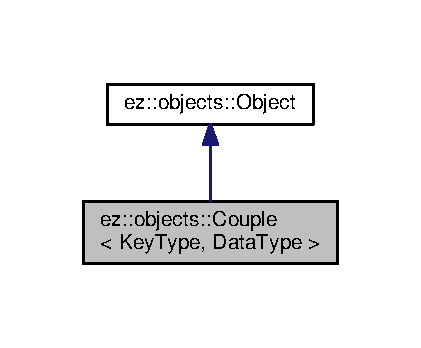
\includegraphics[width=202pt]{classez_1_1objects_1_1Couple__inherit__graph}
\end{center}
\end{figure}


Collaboration diagram for ez\+:\+:objects\+:\+:Couple$<$ Key\+Type, Data\+Type $>$\+:
\nopagebreak
\begin{figure}[H]
\begin{center}
\leavevmode
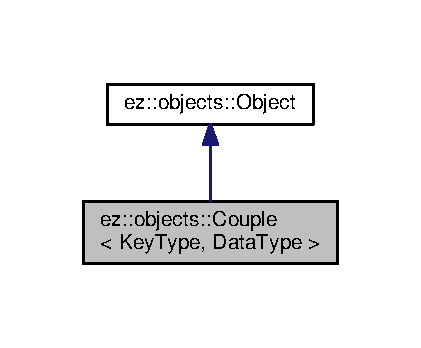
\includegraphics[width=202pt]{classez_1_1objects_1_1Couple__coll__graph}
\end{center}
\end{figure}
\subsection*{Public Types}
\begin{DoxyCompactItemize}
\item 
\mbox{\Hypertarget{classez_1_1objects_1_1Couple_a915baba486e88764cfdfa76dacdadf42}\label{classez_1_1objects_1_1Couple_a915baba486e88764cfdfa76dacdadf42}} 
typedef \hyperlink{classez_1_1objects_1_1Couple}{Couple}$<$ Key\+Type, Data\+Type $>$ {\bfseries self}
\end{DoxyCompactItemize}
\subsection*{Public Member Functions}
\begin{DoxyCompactItemize}
\item 
\mbox{\Hypertarget{classez_1_1objects_1_1Couple_acd2e20b5517b26e706422b8ae8cd057d}\label{classez_1_1objects_1_1Couple_acd2e20b5517b26e706422b8ae8cd057d}} 
{\bfseries Couple} (Key\+Type key, Data\+Type value)
\item 
\mbox{\Hypertarget{classez_1_1objects_1_1Couple_aaba5bcdeaa9e0fc1db029ebc4461d6ed}\label{classez_1_1objects_1_1Couple_aaba5bcdeaa9e0fc1db029ebc4461d6ed}} 
{\bfseries Couple} (const \hyperlink{classez_1_1objects_1_1Couple}{self} \&obj)
\item 
\mbox{\Hypertarget{classez_1_1objects_1_1Couple_a0c08f038504e934e85c9d09259485e48}\label{classez_1_1objects_1_1Couple_a0c08f038504e934e85c9d09259485e48}} 
\hyperlink{classez_1_1objects_1_1Couple}{self} \& {\bfseries operator=} (const \hyperlink{classez_1_1objects_1_1Couple}{self} \&obj)
\item 
\mbox{\Hypertarget{classez_1_1objects_1_1Couple_a09ee264ed12d54a23754647093547f4b}\label{classez_1_1objects_1_1Couple_a09ee264ed12d54a23754647093547f4b}} 
Key\+Type {\bfseries key} ()
\item 
\mbox{\Hypertarget{classez_1_1objects_1_1Couple_ad4a097e8ae5cd40ede29e42f07c37308}\label{classez_1_1objects_1_1Couple_ad4a097e8ae5cd40ede29e42f07c37308}} 
Data\+Type {\bfseries value} ()
\item 
\mbox{\Hypertarget{classez_1_1objects_1_1Couple_afcadb12392164022eaf614c61ccf0eb7}\label{classez_1_1objects_1_1Couple_afcadb12392164022eaf614c61ccf0eb7}} 
void {\bfseries key} (Key\+Type key)
\item 
\mbox{\Hypertarget{classez_1_1objects_1_1Couple_af8c5fd127c385aef53c6a2028558e04c}\label{classez_1_1objects_1_1Couple_af8c5fd127c385aef53c6a2028558e04c}} 
void {\bfseries value} (Data\+Type value)
\item 
void \hyperlink{classez_1_1objects_1_1Couple_ab419858cd3ca8fa27f637ece04d52a97}{print} (std\+::ostream \&stream)
\item 
void \hyperlink{classez_1_1objects_1_1Couple_a7d64b5194ac6092bc553d97fedbe23ad}{output} (std\+::ostream \&stream) override
\item 
void \hyperlink{classez_1_1objects_1_1Couple_a4f7228308e803711bd6866c367e18d06}{input} (std\+::istream \&stream) override
\item 
integer \hyperlink{classez_1_1objects_1_1Couple_a0f4afb11f854f2e84fd2d413cd08212e}{compare} (const \hyperlink{classez_1_1objects_1_1Object}{Object} \&y) override
\item 
\hyperlink{classez_1_1objects_1_1Object}{Object} $\ast$ \hyperlink{classez_1_1objects_1_1Couple_ad258aa010ee9a4bfdecb715de7d93116}{clone} () override
\item 
\hyperlink{classez_1_1objects_1_1Couple}{self} \& \hyperlink{classez_1_1objects_1_1Couple_acd9d9661211e6623461c3c7b2bd37e42}{operator++} ()
\item 
\hyperlink{classez_1_1objects_1_1Couple}{self} \hyperlink{classez_1_1objects_1_1Couple_aae38d565e36c47a0a7fceaf6abbdf9ec}{operator++} (int junk)
\end{DoxyCompactItemize}
\subsection*{Data Fields}
\begin{DoxyCompactItemize}
\item 
\mbox{\Hypertarget{classez_1_1objects_1_1Couple_a16bebe415cd876034d0d230dc00d3faf}\label{classez_1_1objects_1_1Couple_a16bebe415cd876034d0d230dc00d3faf}} 
Key\+Type {\bfseries t\+\_\+key}
\item 
\mbox{\Hypertarget{classez_1_1objects_1_1Couple_a76158ad38ee151c7c498c4659ef4b0f7}\label{classez_1_1objects_1_1Couple_a76158ad38ee151c7c498c4659ef4b0f7}} 
Data\+Type {\bfseries t\+\_\+value}
\end{DoxyCompactItemize}
\subsection*{Additional Inherited Members}


\subsection{Member Function Documentation}
\mbox{\Hypertarget{classez_1_1objects_1_1Couple_ad258aa010ee9a4bfdecb715de7d93116}\label{classez_1_1objects_1_1Couple_ad258aa010ee9a4bfdecb715de7d93116}} 
\index{ez\+::objects\+::\+Couple@{ez\+::objects\+::\+Couple}!clone@{clone}}
\index{clone@{clone}!ez\+::objects\+::\+Couple@{ez\+::objects\+::\+Couple}}
\subsubsection{\texorpdfstring{clone()}{clone()}}
{\footnotesize\ttfamily template$<$class Key\+Type, class Data\+Type$>$ \\
\hyperlink{classez_1_1objects_1_1Object}{Object}$\ast$ \hyperlink{classez_1_1objects_1_1Couple}{ez\+::objects\+::\+Couple}$<$ Key\+Type, Data\+Type $>$\+::clone (\begin{DoxyParamCaption}{ }\end{DoxyParamCaption})\hspace{0.3cm}{\ttfamily [inline]}, {\ttfamily [override]}, {\ttfamily [virtual]}}

return a copy of the object 

Reimplemented from \hyperlink{classez_1_1objects_1_1Object_acf444b2581d898eb4b8c92c2d5865c9e}{ez\+::objects\+::\+Object}.

\mbox{\Hypertarget{classez_1_1objects_1_1Couple_a0f4afb11f854f2e84fd2d413cd08212e}\label{classez_1_1objects_1_1Couple_a0f4afb11f854f2e84fd2d413cd08212e}} 
\index{ez\+::objects\+::\+Couple@{ez\+::objects\+::\+Couple}!compare@{compare}}
\index{compare@{compare}!ez\+::objects\+::\+Couple@{ez\+::objects\+::\+Couple}}
\subsubsection{\texorpdfstring{compare()}{compare()}}
{\footnotesize\ttfamily template$<$class Key\+Type, class Data\+Type$>$ \\
integer \hyperlink{classez_1_1objects_1_1Couple}{ez\+::objects\+::\+Couple}$<$ Key\+Type, Data\+Type $>$\+::compare (\begin{DoxyParamCaption}\item[{const \hyperlink{classez_1_1objects_1_1Object}{Object} \&}]{y }\end{DoxyParamCaption})\hspace{0.3cm}{\ttfamily [inline]}, {\ttfamily [override]}, {\ttfamily [virtual]}}

compare two objects \begin{DoxyReturn}{Returns}
0 if objects are identical, negative value if this $<$ y, positive value if this $>$ y 
\end{DoxyReturn}


Reimplemented from \hyperlink{classez_1_1objects_1_1Object_aca311d389dffa204e425463145f4e1e6}{ez\+::objects\+::\+Object}.

\mbox{\Hypertarget{classez_1_1objects_1_1Couple_a4f7228308e803711bd6866c367e18d06}\label{classez_1_1objects_1_1Couple_a4f7228308e803711bd6866c367e18d06}} 
\index{ez\+::objects\+::\+Couple@{ez\+::objects\+::\+Couple}!input@{input}}
\index{input@{input}!ez\+::objects\+::\+Couple@{ez\+::objects\+::\+Couple}}
\subsubsection{\texorpdfstring{input()}{input()}}
{\footnotesize\ttfamily template$<$class Key\+Type, class Data\+Type$>$ \\
void \hyperlink{classez_1_1objects_1_1Couple}{ez\+::objects\+::\+Couple}$<$ Key\+Type, Data\+Type $>$\+::input (\begin{DoxyParamCaption}\item[{std\+::istream \&}]{stream }\end{DoxyParamCaption})\hspace{0.3cm}{\ttfamily [inline]}, {\ttfamily [override]}, {\ttfamily [virtual]}}

this function is used to get the data field members of an object from a stream and acts as unserialize 

Reimplemented from \hyperlink{classez_1_1objects_1_1Object_a878bdc53b7f16fda6fa15dab214c4b6a}{ez\+::objects\+::\+Object}.

\mbox{\Hypertarget{classez_1_1objects_1_1Couple_acd9d9661211e6623461c3c7b2bd37e42}\label{classez_1_1objects_1_1Couple_acd9d9661211e6623461c3c7b2bd37e42}} 
\index{ez\+::objects\+::\+Couple@{ez\+::objects\+::\+Couple}!operator++@{operator++}}
\index{operator++@{operator++}!ez\+::objects\+::\+Couple@{ez\+::objects\+::\+Couple}}
\subsubsection{\texorpdfstring{operator++()}{operator++()}\hspace{0.1cm}{\footnotesize\ttfamily [1/2]}}
{\footnotesize\ttfamily template$<$class Key\+Type, class Data\+Type$>$ \\
\hyperlink{classez_1_1objects_1_1Couple}{self}\& \hyperlink{classez_1_1objects_1_1Couple}{ez\+::objects\+::\+Couple}$<$ Key\+Type, Data\+Type $>$\+::operator++ (\begin{DoxyParamCaption}{ }\end{DoxyParamCaption})\hspace{0.3cm}{\ttfamily [inline]}}

increment operator, needed because of method iota of \hyperlink{classez_1_1objects_1_1Vector}{Vector} which uses value++ \mbox{\Hypertarget{classez_1_1objects_1_1Couple_aae38d565e36c47a0a7fceaf6abbdf9ec}\label{classez_1_1objects_1_1Couple_aae38d565e36c47a0a7fceaf6abbdf9ec}} 
\index{ez\+::objects\+::\+Couple@{ez\+::objects\+::\+Couple}!operator++@{operator++}}
\index{operator++@{operator++}!ez\+::objects\+::\+Couple@{ez\+::objects\+::\+Couple}}
\subsubsection{\texorpdfstring{operator++()}{operator++()}\hspace{0.1cm}{\footnotesize\ttfamily [2/2]}}
{\footnotesize\ttfamily template$<$class Key\+Type, class Data\+Type$>$ \\
\hyperlink{classez_1_1objects_1_1Couple}{self} \hyperlink{classez_1_1objects_1_1Couple}{ez\+::objects\+::\+Couple}$<$ Key\+Type, Data\+Type $>$\+::operator++ (\begin{DoxyParamCaption}\item[{int}]{junk }\end{DoxyParamCaption})\hspace{0.3cm}{\ttfamily [inline]}}

increment operator, needed because of method iota of \hyperlink{classez_1_1objects_1_1Vector}{Vector} which uses value++ \mbox{\Hypertarget{classez_1_1objects_1_1Couple_a7d64b5194ac6092bc553d97fedbe23ad}\label{classez_1_1objects_1_1Couple_a7d64b5194ac6092bc553d97fedbe23ad}} 
\index{ez\+::objects\+::\+Couple@{ez\+::objects\+::\+Couple}!output@{output}}
\index{output@{output}!ez\+::objects\+::\+Couple@{ez\+::objects\+::\+Couple}}
\subsubsection{\texorpdfstring{output()}{output()}}
{\footnotesize\ttfamily template$<$class Key\+Type, class Data\+Type$>$ \\
void \hyperlink{classez_1_1objects_1_1Couple}{ez\+::objects\+::\+Couple}$<$ Key\+Type, Data\+Type $>$\+::output (\begin{DoxyParamCaption}\item[{std\+::ostream \&}]{stream }\end{DoxyParamCaption})\hspace{0.3cm}{\ttfamily [inline]}, {\ttfamily [override]}, {\ttfamily [virtual]}}

this function is used to print the contents of the object in a serializable manner 

Reimplemented from \hyperlink{classez_1_1objects_1_1Object_a0fdfe18e6c35d6b0d7e7a01265aded15}{ez\+::objects\+::\+Object}.

\mbox{\Hypertarget{classez_1_1objects_1_1Couple_ab419858cd3ca8fa27f637ece04d52a97}\label{classez_1_1objects_1_1Couple_ab419858cd3ca8fa27f637ece04d52a97}} 
\index{ez\+::objects\+::\+Couple@{ez\+::objects\+::\+Couple}!print@{print}}
\index{print@{print}!ez\+::objects\+::\+Couple@{ez\+::objects\+::\+Couple}}
\subsubsection{\texorpdfstring{print()}{print()}}
{\footnotesize\ttfamily template$<$class Key\+Type, class Data\+Type$>$ \\
void \hyperlink{classez_1_1objects_1_1Couple}{ez\+::objects\+::\+Couple}$<$ Key\+Type, Data\+Type $>$\+::print (\begin{DoxyParamCaption}\item[{std\+::ostream \&}]{stream }\end{DoxyParamCaption})\hspace{0.3cm}{\ttfamily [inline]}, {\ttfamily [virtual]}}

this function is used to print the contents of the object in a human readable format 
\begin{DoxyParams}{Parameters}
{\em stream} & output stream for example std\+::cout \\
\hline
\end{DoxyParams}


Reimplemented from \hyperlink{classez_1_1objects_1_1Object_a9e20f39a78163f67f000576149d858b3}{ez\+::objects\+::\+Object}.



The documentation for this class was generated from the following file\+:\begin{DoxyCompactItemize}
\item 
src/version\+\_\+2018.\+06/objects/couple.\+h\end{DoxyCompactItemize}

\hypertarget{classez_1_1essential_1_1CPUTimer}{}\section{ez\+:\+:essential\+:\+:C\+P\+U\+Timer Class Reference}
\label{classez_1_1essential_1_1CPUTimer}\index{ez\+::essential\+::\+C\+P\+U\+Timer@{ez\+::essential\+::\+C\+P\+U\+Timer}}


{\ttfamily \#include $<$cpu\+\_\+timer.\+h$>$}

\subsection*{Public Types}
\begin{DoxyCompactItemize}
\item 
\mbox{\Hypertarget{classez_1_1essential_1_1CPUTimer_accb93c3ac1ba89c9dceedd765f4a11ee}\label{classez_1_1essential_1_1CPUTimer_accb93c3ac1ba89c9dceedd765f4a11ee}} 
typedef std\+::chrono\+::time\+\_\+point$<$ std\+::chrono\+::high\+\_\+resolution\+\_\+clock $>$ {\bfseries Time}
\item 
\mbox{\Hypertarget{classez_1_1essential_1_1CPUTimer_ac07c2f4cfa8f31ae7a99345178d8deba}\label{classez_1_1essential_1_1CPUTimer_ac07c2f4cfa8f31ae7a99345178d8deba}} 
typedef std\+::chrono\+::milliseconds {\bfseries millis}
\end{DoxyCompactItemize}
\subsection*{Public Member Functions}
\begin{DoxyCompactItemize}
\item 
\hyperlink{classez_1_1essential_1_1CPUTimer_aa06f8e13b3c82bbb8642f4981bfff7e7}{C\+P\+U\+Timer} ()
\item 
void \hyperlink{classez_1_1essential_1_1CPUTimer_a2117cc7fd9f933bb0c6d28fdf9a9f74a}{start} ()
\item 
void \hyperlink{classez_1_1essential_1_1CPUTimer_a318dfb72b3b7e61ab90ea3699e7d66a6}{stop} ()
\item 
long\+\_\+integer \hyperlink{classez_1_1essential_1_1CPUTimer_a4a8a5f9a298400052e54c0219ff254c2}{get\+\_\+milli\+\_\+seconds} ()
\item 
long\+\_\+integer \hyperlink{classez_1_1essential_1_1CPUTimer_a5514bcd6ee6e46961b66497bf5b27751}{get\+\_\+seconds} ()
\item 
long\+\_\+integer \hyperlink{classez_1_1essential_1_1CPUTimer_a867ed5183849fa164f01a035b04e0ad5}{get\+\_\+seconds\+\_\+elapsed} ()
\item 
\mbox{\Hypertarget{classez_1_1essential_1_1CPUTimer_a4fc87e7c3591adf9fec42917caa38464}\label{classez_1_1essential_1_1CPUTimer_a4fc87e7c3591adf9fec42917caa38464}} 
ostream \& {\bfseries print} (ostream \&out)
\end{DoxyCompactItemize}
\subsection*{Data Fields}
\begin{DoxyCompactItemize}
\item 
\mbox{\Hypertarget{classez_1_1essential_1_1CPUTimer_a9153ec33fb7ea258b0633eb183d792d1}\label{classez_1_1essential_1_1CPUTimer_a9153ec33fb7ea258b0633eb183d792d1}} 
Time {\bfseries event\+\_\+start}
\item 
\mbox{\Hypertarget{classez_1_1essential_1_1CPUTimer_a3b76f40057f1d012e4c33a4923047923}\label{classez_1_1essential_1_1CPUTimer_a3b76f40057f1d012e4c33a4923047923}} 
Time {\bfseries event\+\_\+stop}
\end{DoxyCompactItemize}
\subsection*{Friends}
\begin{DoxyCompactItemize}
\item 
\mbox{\Hypertarget{classez_1_1essential_1_1CPUTimer_a50a6415ed758f854d5211347e860452a}\label{classez_1_1essential_1_1CPUTimer_a50a6415ed758f854d5211347e860452a}} 
ostream \& {\bfseries operator$<$$<$} (ostream \&out, \hyperlink{classez_1_1essential_1_1CPUTimer}{C\+P\+U\+Timer} \&c)
\end{DoxyCompactItemize}


\subsection{Detailed Description}
class used to measure performances of algorithms. 
\begin{DoxyItemize}
\item use \hyperlink{classez_1_1essential_1_1CPUTimer_a2117cc7fd9f933bb0c6d28fdf9a9f74a}{start()} method to start timer 
\item use \hyperlink{classez_1_1essential_1_1CPUTimer_a318dfb72b3b7e61ab90ea3699e7d66a6}{stop()} method to stop 
\item use \hyperlink{classez_1_1essential_1_1CPUTimer_a5514bcd6ee6e46961b66497bf5b27751}{get\+\_\+seconds()} method to obtain the number of seconds between start and stop 
\end{DoxyItemize}

\subsection{Constructor \& Destructor Documentation}
\mbox{\Hypertarget{classez_1_1essential_1_1CPUTimer_aa06f8e13b3c82bbb8642f4981bfff7e7}\label{classez_1_1essential_1_1CPUTimer_aa06f8e13b3c82bbb8642f4981bfff7e7}} 
\index{ez\+::essential\+::\+C\+P\+U\+Timer@{ez\+::essential\+::\+C\+P\+U\+Timer}!C\+P\+U\+Timer@{C\+P\+U\+Timer}}
\index{C\+P\+U\+Timer@{C\+P\+U\+Timer}!ez\+::essential\+::\+C\+P\+U\+Timer@{ez\+::essential\+::\+C\+P\+U\+Timer}}
\subsubsection{\texorpdfstring{C\+P\+U\+Timer()}{CPUTimer()}}
{\footnotesize\ttfamily C\+P\+U\+Timer\+::\+C\+P\+U\+Timer (\begin{DoxyParamCaption}{ }\end{DoxyParamCaption})}

default constructor 

\subsection{Member Function Documentation}
\mbox{\Hypertarget{classez_1_1essential_1_1CPUTimer_a4a8a5f9a298400052e54c0219ff254c2}\label{classez_1_1essential_1_1CPUTimer_a4a8a5f9a298400052e54c0219ff254c2}} 
\index{ez\+::essential\+::\+C\+P\+U\+Timer@{ez\+::essential\+::\+C\+P\+U\+Timer}!get\+\_\+milli\+\_\+seconds@{get\+\_\+milli\+\_\+seconds}}
\index{get\+\_\+milli\+\_\+seconds@{get\+\_\+milli\+\_\+seconds}!ez\+::essential\+::\+C\+P\+U\+Timer@{ez\+::essential\+::\+C\+P\+U\+Timer}}
\subsubsection{\texorpdfstring{get\+\_\+milli\+\_\+seconds()}{get\_milli\_seconds()}}
{\footnotesize\ttfamily long\+\_\+integer C\+P\+U\+Timer\+::get\+\_\+milli\+\_\+seconds (\begin{DoxyParamCaption}{ }\end{DoxyParamCaption})}

get number of milli seconds from start to stop events \mbox{\Hypertarget{classez_1_1essential_1_1CPUTimer_a5514bcd6ee6e46961b66497bf5b27751}\label{classez_1_1essential_1_1CPUTimer_a5514bcd6ee6e46961b66497bf5b27751}} 
\index{ez\+::essential\+::\+C\+P\+U\+Timer@{ez\+::essential\+::\+C\+P\+U\+Timer}!get\+\_\+seconds@{get\+\_\+seconds}}
\index{get\+\_\+seconds@{get\+\_\+seconds}!ez\+::essential\+::\+C\+P\+U\+Timer@{ez\+::essential\+::\+C\+P\+U\+Timer}}
\subsubsection{\texorpdfstring{get\+\_\+seconds()}{get\_seconds()}}
{\footnotesize\ttfamily long\+\_\+integer C\+P\+U\+Timer\+::get\+\_\+seconds (\begin{DoxyParamCaption}{ }\end{DoxyParamCaption})}

get number of seconds from start to stop events \mbox{\Hypertarget{classez_1_1essential_1_1CPUTimer_a867ed5183849fa164f01a035b04e0ad5}\label{classez_1_1essential_1_1CPUTimer_a867ed5183849fa164f01a035b04e0ad5}} 
\index{ez\+::essential\+::\+C\+P\+U\+Timer@{ez\+::essential\+::\+C\+P\+U\+Timer}!get\+\_\+seconds\+\_\+elapsed@{get\+\_\+seconds\+\_\+elapsed}}
\index{get\+\_\+seconds\+\_\+elapsed@{get\+\_\+seconds\+\_\+elapsed}!ez\+::essential\+::\+C\+P\+U\+Timer@{ez\+::essential\+::\+C\+P\+U\+Timer}}
\subsubsection{\texorpdfstring{get\+\_\+seconds\+\_\+elapsed()}{get\_seconds\_elapsed()}}
{\footnotesize\ttfamily long\+\_\+integer C\+P\+U\+Timer\+::get\+\_\+seconds\+\_\+elapsed (\begin{DoxyParamCaption}{ }\end{DoxyParamCaption})}

get number of seconds since start event \mbox{\Hypertarget{classez_1_1essential_1_1CPUTimer_a2117cc7fd9f933bb0c6d28fdf9a9f74a}\label{classez_1_1essential_1_1CPUTimer_a2117cc7fd9f933bb0c6d28fdf9a9f74a}} 
\index{ez\+::essential\+::\+C\+P\+U\+Timer@{ez\+::essential\+::\+C\+P\+U\+Timer}!start@{start}}
\index{start@{start}!ez\+::essential\+::\+C\+P\+U\+Timer@{ez\+::essential\+::\+C\+P\+U\+Timer}}
\subsubsection{\texorpdfstring{start()}{start()}}
{\footnotesize\ttfamily void C\+P\+U\+Timer\+::start (\begin{DoxyParamCaption}{ }\end{DoxyParamCaption})}

start chrono and record clocks \mbox{\Hypertarget{classez_1_1essential_1_1CPUTimer_a318dfb72b3b7e61ab90ea3699e7d66a6}\label{classez_1_1essential_1_1CPUTimer_a318dfb72b3b7e61ab90ea3699e7d66a6}} 
\index{ez\+::essential\+::\+C\+P\+U\+Timer@{ez\+::essential\+::\+C\+P\+U\+Timer}!stop@{stop}}
\index{stop@{stop}!ez\+::essential\+::\+C\+P\+U\+Timer@{ez\+::essential\+::\+C\+P\+U\+Timer}}
\subsubsection{\texorpdfstring{stop()}{stop()}}
{\footnotesize\ttfamily void C\+P\+U\+Timer\+::stop (\begin{DoxyParamCaption}{ }\end{DoxyParamCaption})}

stop chrono and record clocks 

The documentation for this class was generated from the following files\+:\begin{DoxyCompactItemize}
\item 
src/version\+\_\+2018.\+06/essential/cpu\+\_\+timer.\+h\item 
src/version\+\_\+2018.\+06/essential/cpu\+\_\+timer.\+cpp\end{DoxyCompactItemize}

\hypertarget{classez_1_1io_1_1CSVFile}{}\section{ez\+:\+:io\+:\+:C\+S\+V\+File Class Reference}
\label{classez_1_1io_1_1CSVFile}\index{ez\+::io\+::\+C\+S\+V\+File@{ez\+::io\+::\+C\+S\+V\+File}}
\subsection*{Public Member Functions}
\begin{DoxyCompactItemize}
\item 
\mbox{\Hypertarget{classez_1_1io_1_1CSVFile_aab1cc6fb7d8eae0ea5a0f57f1485e9b5}\label{classez_1_1io_1_1CSVFile_aab1cc6fb7d8eae0ea5a0f57f1485e9b5}} 
{\bfseries C\+S\+V\+File} (std\+::string \+\_\+file\+\_\+name)
\item 
\mbox{\Hypertarget{classez_1_1io_1_1CSVFile_a84c8046d38d948e93c062546492ccbaa}\label{classez_1_1io_1_1CSVFile_a84c8046d38d948e93c062546492ccbaa}} 
void {\bfseries read} (std\+::string field\+\_\+delimiter=\char`\"{},\char`\"{}, std\+::string string\+\_\+delimiter=\char`\"{}\textbackslash{})
\item 
\mbox{\Hypertarget{classez_1_1io_1_1CSVFile_a862894d8b84c39a2a35a339f3c0341cb}\label{classez_1_1io_1_1CSVFile_a862894d8b84c39a2a35a339f3c0341cb}} 
std\+::vector$<$ std\+::vector$<$ std\+::string $>$ $>$ \& {\bfseries get\+\_\+data} ()
\end{DoxyCompactItemize}
\subsection*{Protected Attributes}
\begin{DoxyCompactItemize}
\item 
\mbox{\Hypertarget{classez_1_1io_1_1CSVFile_ae37f393dbc90ba6397702bc543a2b4da}\label{classez_1_1io_1_1CSVFile_ae37f393dbc90ba6397702bc543a2b4da}} 
std\+::string {\bfseries file\+\_\+name}
\item 
\mbox{\Hypertarget{classez_1_1io_1_1CSVFile_ae73026e2bda2371a557f96ff61134ad9}\label{classez_1_1io_1_1CSVFile_ae73026e2bda2371a557f96ff61134ad9}} 
std\+::vector$<$ std\+::vector$<$ std\+::string $>$ $>$ {\bfseries data}
\end{DoxyCompactItemize}


The documentation for this class was generated from the following files\+:\begin{DoxyCompactItemize}
\item 
src/version\+\_\+2018.\+06/io/csv\+\_\+file.\+h\item 
src/version\+\_\+2018.\+06/io/csv\+\_\+file.\+cpp\end{DoxyCompactItemize}

\hypertarget{classez_1_1trees_1_1DynamicBinaryNode}{}\section{ez\+:\+:trees\+:\+:Dynamic\+Binary\+Node Class Reference}
\label{classez_1_1trees_1_1DynamicBinaryNode}\index{ez\+::trees\+::\+Dynamic\+Binary\+Node@{ez\+::trees\+::\+Dynamic\+Binary\+Node}}


Collaboration diagram for ez\+:\+:trees\+:\+:Dynamic\+Binary\+Node\+:
\nopagebreak
\begin{figure}[H]
\begin{center}
\leavevmode
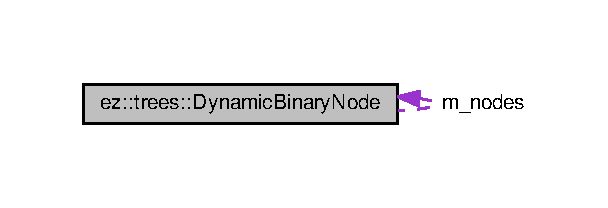
\includegraphics[width=292pt]{classez_1_1trees_1_1DynamicBinaryNode__coll__graph}
\end{center}
\end{figure}
\subsection*{Public Types}
\begin{DoxyCompactItemize}
\item 
\mbox{\Hypertarget{classez_1_1trees_1_1DynamicBinaryNode_a4bcbddfe8cdea01a78faab44a00ccc54}\label{classez_1_1trees_1_1DynamicBinaryNode_a4bcbddfe8cdea01a78faab44a00ccc54}} 
enum \{ {\bfseries L\+E\+FT} = 0, 
{\bfseries R\+I\+G\+HT} = 1, 
{\bfseries P\+A\+R\+E\+NT} = 2, 
{\bfseries A\+L\+I\+G\+N\+M\+E\+NT} = 4
 \}
\item 
\mbox{\Hypertarget{classez_1_1trees_1_1DynamicBinaryNode_a2bcb4fe8c63f5fe47a2aa49dd8e7d803}\label{classez_1_1trees_1_1DynamicBinaryNode_a2bcb4fe8c63f5fe47a2aa49dd8e7d803}} 
typedef \hyperlink{classez_1_1trees_1_1DynamicBinaryNode}{Dynamic\+Binary\+Node} {\bfseries self}
\end{DoxyCompactItemize}
\subsection*{Public Member Functions}
\begin{DoxyCompactItemize}
\item 
\mbox{\Hypertarget{classez_1_1trees_1_1DynamicBinaryNode_a3c0aff288f8151d65a1f5f6cd6f3de5b}\label{classez_1_1trees_1_1DynamicBinaryNode_a3c0aff288f8151d65a1f5f6cd6f3de5b}} 
{\bfseries Dynamic\+Binary\+Node} (const \hyperlink{classez_1_1trees_1_1DynamicNode}{Dynamic\+Node} \&obj)
\item 
\mbox{\Hypertarget{classez_1_1trees_1_1DynamicBinaryNode_a6e1ee2312112126c382862a7351fe9e9}\label{classez_1_1trees_1_1DynamicBinaryNode_a6e1ee2312112126c382862a7351fe9e9}} 
\hyperlink{classez_1_1trees_1_1DynamicBinaryNode}{Dynamic\+Binary\+Node} \& {\bfseries operator=} (const \hyperlink{classez_1_1trees_1_1DynamicBinaryNode}{Dynamic\+Binary\+Node} \&obj)
\item 
\mbox{\Hypertarget{classez_1_1trees_1_1DynamicBinaryNode_a37991401d8e59e511c961063ffba0b75}\label{classez_1_1trees_1_1DynamicBinaryNode_a37991401d8e59e511c961063ffba0b75}} 
\hyperlink{classez_1_1trees_1_1DynamicBinaryNode}{self} $\ast$ {\bfseries clone} ()
\item 
\mbox{\Hypertarget{classez_1_1trees_1_1DynamicBinaryNode_a466a8d0334eaa62aefe514d7de13553e}\label{classez_1_1trees_1_1DynamicBinaryNode_a466a8d0334eaa62aefe514d7de13553e}} 
void {\bfseries clean} ()
\item 
\mbox{\Hypertarget{classez_1_1trees_1_1DynamicBinaryNode_a09006260f87e7df96c64a75eb79fc834}\label{classez_1_1trees_1_1DynamicBinaryNode_a09006260f87e7df96c64a75eb79fc834}} 
bool {\bfseries is\+\_\+root} ()
\item 
\mbox{\Hypertarget{classez_1_1trees_1_1DynamicBinaryNode_abd663d6ed47256c1177a2ff17b89c041}\label{classez_1_1trees_1_1DynamicBinaryNode_abd663d6ed47256c1177a2ff17b89c041}} 
bool {\bfseries is\+\_\+leaf} ()
\item 
\mbox{\Hypertarget{classez_1_1trees_1_1DynamicBinaryNode_adf14c1f0dddfa44a1e569be4c7e117f8}\label{classez_1_1trees_1_1DynamicBinaryNode_adf14c1f0dddfa44a1e569be4c7e117f8}} 
\hyperlink{classez_1_1trees_1_1DynamicBinaryNode}{self} $\ast$ {\bfseries parent} ()
\item 
\mbox{\Hypertarget{classez_1_1trees_1_1DynamicBinaryNode_a345ab5ff3a728a6c5f8105204b8fb236}\label{classez_1_1trees_1_1DynamicBinaryNode_a345ab5ff3a728a6c5f8105204b8fb236}} 
void {\bfseries parent} (\hyperlink{classez_1_1trees_1_1DynamicBinaryNode}{self} $\ast$parent)
\item 
\mbox{\Hypertarget{classez_1_1trees_1_1DynamicBinaryNode_a7e9014c242db90f7cd0fafb5275233f7}\label{classez_1_1trees_1_1DynamicBinaryNode_a7e9014c242db90f7cd0fafb5275233f7}} 
\hyperlink{classez_1_1trees_1_1DynamicBinaryNode}{self} $\ast$ {\bfseries left} ()
\item 
\mbox{\Hypertarget{classez_1_1trees_1_1DynamicBinaryNode_ad275bb66c740e4786c21887e30648e64}\label{classez_1_1trees_1_1DynamicBinaryNode_ad275bb66c740e4786c21887e30648e64}} 
void {\bfseries left} (\hyperlink{classez_1_1trees_1_1DynamicBinaryNode}{self} $\ast$node)
\item 
\mbox{\Hypertarget{classez_1_1trees_1_1DynamicBinaryNode_a904fe4dfe5022d7672deb92557ee3af0}\label{classez_1_1trees_1_1DynamicBinaryNode_a904fe4dfe5022d7672deb92557ee3af0}} 
\hyperlink{classez_1_1trees_1_1DynamicBinaryNode}{self} $\ast$ {\bfseries right} ()
\item 
\mbox{\Hypertarget{classez_1_1trees_1_1DynamicBinaryNode_acfbaaa7d90ea693d5001eb620a26a1e4}\label{classez_1_1trees_1_1DynamicBinaryNode_acfbaaa7d90ea693d5001eb620a26a1e4}} 
void {\bfseries right} (\hyperlink{classez_1_1trees_1_1DynamicBinaryNode}{self} $\ast$node)
\item 
\mbox{\Hypertarget{classez_1_1trees_1_1DynamicBinaryNode_ae6899f68096ad9f547681e72941afcfd}\label{classez_1_1trees_1_1DynamicBinaryNode_ae6899f68096ad9f547681e72941afcfd}} 
void {\bfseries print} (std\+::ostream \&out)
\item 
\mbox{\Hypertarget{classez_1_1trees_1_1DynamicBinaryNode_ae3d58157576c3032d8511adde0ba27d9}\label{classez_1_1trees_1_1DynamicBinaryNode_ae3d58157576c3032d8511adde0ba27d9}} 
void {\bfseries check} ()
\item 
\mbox{\Hypertarget{classez_1_1trees_1_1DynamicBinaryNode_a586c07184371b9565272aa198cd2dc8f}\label{classez_1_1trees_1_1DynamicBinaryNode_a586c07184371b9565272aa198cd2dc8f}} 
void {\bfseries internals} (vector$<$ \hyperlink{classez_1_1trees_1_1DynamicBinaryNode}{self} $\ast$$>$ \&v)
\item 
\mbox{\Hypertarget{classez_1_1trees_1_1DynamicBinaryNode_a92cc6e99c99839e41168232eddae509b}\label{classez_1_1trees_1_1DynamicBinaryNode_a92cc6e99c99839e41168232eddae509b}} 
void {\bfseries externals} (vector$<$ \hyperlink{classez_1_1trees_1_1DynamicBinaryNode}{self} $\ast$$>$ \&v)
\item 
\mbox{\Hypertarget{classez_1_1trees_1_1DynamicBinaryNode_a72d1a18044d42191f8cc927e4782e379}\label{classez_1_1trees_1_1DynamicBinaryNode_a72d1a18044d42191f8cc927e4782e379}} 
void {\bfseries all\+\_\+nodes} (vector$<$ \hyperlink{classez_1_1trees_1_1DynamicBinaryNode}{self} $\ast$$>$ \&v)
\end{DoxyCompactItemize}
\subsection*{Data Fields}
\begin{DoxyCompactItemize}
\item 
\mbox{\Hypertarget{classez_1_1trees_1_1DynamicBinaryNode_abe1ece54d3b2fcafcde7b153ca367506}\label{classez_1_1trees_1_1DynamicBinaryNode_abe1ece54d3b2fcafcde7b153ca367506}} 
\hyperlink{classez_1_1trees_1_1DynamicBinaryNode}{self} $\ast$ {\bfseries m\+\_\+nodes} \mbox{[}A\+L\+I\+G\+N\+M\+E\+NT\mbox{]}
\end{DoxyCompactItemize}
\subsection*{Friends}
\begin{DoxyCompactItemize}
\item 
\mbox{\Hypertarget{classez_1_1trees_1_1DynamicBinaryNode_aa1d826e7fbedbc2b2358e08bc03fc894}\label{classez_1_1trees_1_1DynamicBinaryNode_aa1d826e7fbedbc2b2358e08bc03fc894}} 
std\+::ostream \& {\bfseries operator$<$$<$} (std\+::ostream \&out, \hyperlink{classez_1_1trees_1_1DynamicBinaryNode}{self} \&obj)
\end{DoxyCompactItemize}


The documentation for this class was generated from the following files\+:\begin{DoxyCompactItemize}
\item 
src/version\+\_\+2018.\+06/trees/dynamic\+\_\+binary\+\_\+node.\+h\item 
src/version\+\_\+2018.\+06/trees/dynamic\+\_\+binary\+\_\+node.\+cpp\end{DoxyCompactItemize}

\hypertarget{classez_1_1trees_1_1DynamicBinaryTree}{}\section{ez\+:\+:trees\+:\+:Dynamic\+Binary\+Tree Class Reference}
\label{classez_1_1trees_1_1DynamicBinaryTree}\index{ez\+::trees\+::\+Dynamic\+Binary\+Tree@{ez\+::trees\+::\+Dynamic\+Binary\+Tree}}


Inheritance diagram for ez\+:\+:trees\+:\+:Dynamic\+Binary\+Tree\+:
\nopagebreak
\begin{figure}[H]
\begin{center}
\leavevmode
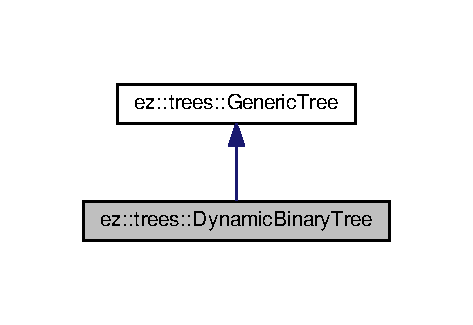
\includegraphics[width=227pt]{classez_1_1trees_1_1DynamicBinaryTree__inherit__graph}
\end{center}
\end{figure}


Collaboration diagram for ez\+:\+:trees\+:\+:Dynamic\+Binary\+Tree\+:
\nopagebreak
\begin{figure}[H]
\begin{center}
\leavevmode
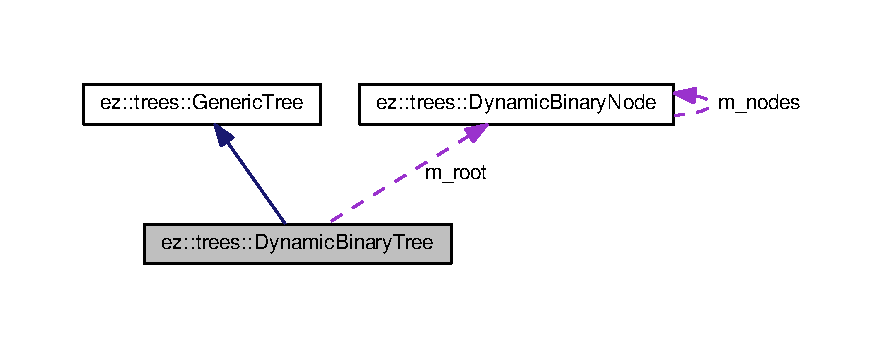
\includegraphics[width=350pt]{classez_1_1trees_1_1DynamicBinaryTree__coll__graph}
\end{center}
\end{figure}
\subsection*{Public Types}
\begin{DoxyCompactItemize}
\item 
\mbox{\Hypertarget{classez_1_1trees_1_1DynamicBinaryTree_a7b76d15a64fbaeb7e1f873fe8fb72669}\label{classez_1_1trees_1_1DynamicBinaryTree_a7b76d15a64fbaeb7e1f873fe8fb72669}} 
typedef \hyperlink{classez_1_1trees_1_1DynamicBinaryTree}{Dynamic\+Binary\+Tree} {\bfseries self}
\item 
\mbox{\Hypertarget{classez_1_1trees_1_1DynamicBinaryTree_ac76c0520ea1117a5222f10d8d4161d05}\label{classez_1_1trees_1_1DynamicBinaryTree_ac76c0520ea1117a5222f10d8d4161d05}} 
typedef \hyperlink{classez_1_1trees_1_1DynamicBinaryNode}{Dynamic\+Binary\+Node} $\ast$ {\bfseries Node}
\end{DoxyCompactItemize}
\subsection*{Public Member Functions}
\begin{DoxyCompactItemize}
\item 
\mbox{\Hypertarget{classez_1_1trees_1_1DynamicBinaryTree_a13d170a17d9c4102e1b5f379e290945e}\label{classez_1_1trees_1_1DynamicBinaryTree_a13d170a17d9c4102e1b5f379e290945e}} 
{\bfseries Dynamic\+Binary\+Tree} (\hyperlink{classez_1_1trees_1_1DynamicBinaryNode}{Node} root)
\item 
\mbox{\Hypertarget{classez_1_1trees_1_1DynamicBinaryTree_a6c73288a9c41faa902e53494264eeb70}\label{classez_1_1trees_1_1DynamicBinaryTree_a6c73288a9c41faa902e53494264eeb70}} 
{\bfseries Dynamic\+Binary\+Tree} (const \hyperlink{classez_1_1trees_1_1DynamicBinaryTree}{Dynamic\+Binary\+Tree} \&obj)
\item 
\mbox{\Hypertarget{classez_1_1trees_1_1DynamicBinaryTree_a913b32bc9d9fd3e3d1dc1efce492cbee}\label{classez_1_1trees_1_1DynamicBinaryTree_a913b32bc9d9fd3e3d1dc1efce492cbee}} 
\hyperlink{classez_1_1trees_1_1DynamicBinaryTree}{Dynamic\+Binary\+Tree} \& {\bfseries operator=} (const \hyperlink{classez_1_1trees_1_1DynamicBinaryTree}{Dynamic\+Binary\+Tree} \&obj)
\item 
\mbox{\Hypertarget{classez_1_1trees_1_1DynamicBinaryTree_a43bddd6ed670fbee68daba77031a2de0}\label{classez_1_1trees_1_1DynamicBinaryTree_a43bddd6ed670fbee68daba77031a2de0}} 
\hyperlink{classez_1_1trees_1_1DynamicBinaryNode}{Node} {\bfseries root} (\hyperlink{classez_1_1trees_1_1DynamicBinaryNode}{Node} root)
\item 
\mbox{\Hypertarget{classez_1_1trees_1_1DynamicBinaryTree_aab35fd04ff76684ac5ec9f3510e98ccb}\label{classez_1_1trees_1_1DynamicBinaryTree_aab35fd04ff76684ac5ec9f3510e98ccb}} 
\hyperlink{classez_1_1trees_1_1DynamicBinaryTree}{Dynamic\+Binary\+Tree} $\ast$ {\bfseries clone} ()
\item 
\mbox{\Hypertarget{classez_1_1trees_1_1DynamicBinaryTree_ae093b35e820a64121edfa4a171f24414}\label{classez_1_1trees_1_1DynamicBinaryTree_ae093b35e820a64121edfa4a171f24414}} 
void {\bfseries internals} (vector$<$ \hyperlink{classez_1_1trees_1_1DynamicBinaryNode}{Node} $>$ \&v)
\item 
\mbox{\Hypertarget{classez_1_1trees_1_1DynamicBinaryTree_a176763055f37802f531152444c6962f9}\label{classez_1_1trees_1_1DynamicBinaryTree_a176763055f37802f531152444c6962f9}} 
void {\bfseries externals} (vector$<$ \hyperlink{classez_1_1trees_1_1DynamicBinaryNode}{Node} $>$ \&v)
\item 
\mbox{\Hypertarget{classez_1_1trees_1_1DynamicBinaryTree_af9204bdfd570e7b987b1edc4b4c796f0}\label{classez_1_1trees_1_1DynamicBinaryTree_af9204bdfd570e7b987b1edc4b4c796f0}} 
void {\bfseries all\+\_\+nodes} (vector$<$ \hyperlink{classez_1_1trees_1_1DynamicBinaryNode}{Node} $>$ \&v)
\item 
\mbox{\Hypertarget{classez_1_1trees_1_1DynamicBinaryTree_a9f323dc1bef791820409359221a1b622}\label{classez_1_1trees_1_1DynamicBinaryTree_a9f323dc1bef791820409359221a1b622}} 
void {\bfseries degraph} (\hyperlink{classez_1_1trees_1_1DynamicBinaryNode}{Node} src)
\item 
\mbox{\Hypertarget{classez_1_1trees_1_1DynamicBinaryTree_a4f1311d938c6a28e11022f27ad82d7aa}\label{classez_1_1trees_1_1DynamicBinaryTree_a4f1311d938c6a28e11022f27ad82d7aa}} 
void {\bfseries regraph} (\hyperlink{classez_1_1trees_1_1DynamicBinaryNode}{Node} src, \hyperlink{classez_1_1trees_1_1DynamicBinaryNode}{Node} dst)
\item 
\mbox{\Hypertarget{classez_1_1trees_1_1DynamicBinaryTree_a991ca1eb03e7095274f3ea32cd4c3b85}\label{classez_1_1trees_1_1DynamicBinaryTree_a991ca1eb03e7095274f3ea32cd4c3b85}} 
void {\bfseries check} ()
\item 
\mbox{\Hypertarget{classez_1_1trees_1_1DynamicBinaryTree_a3688914d22be9094da4e2f4f1bbcb7f2}\label{classez_1_1trees_1_1DynamicBinaryTree_a3688914d22be9094da4e2f4f1bbcb7f2}} 
void {\bfseries print} (std\+::ostream \&out)
\end{DoxyCompactItemize}
\subsection*{Data Fields}
\begin{DoxyCompactItemize}
\item 
\mbox{\Hypertarget{classez_1_1trees_1_1DynamicBinaryTree_a3d1116a396abb48d1ee8378ad7c395d5}\label{classez_1_1trees_1_1DynamicBinaryTree_a3d1116a396abb48d1ee8378ad7c395d5}} 
\hyperlink{classez_1_1trees_1_1DynamicBinaryNode}{Node} {\bfseries m\+\_\+root}
\end{DoxyCompactItemize}


The documentation for this class was generated from the following file\+:\begin{DoxyCompactItemize}
\item 
src/version\+\_\+2018.\+06/trees/dynamic\+\_\+binary\+\_\+tree.\+h\end{DoxyCompactItemize}

\hypertarget{classez_1_1trees_1_1DynamicNode}{}\section{ez\+:\+:trees\+:\+:Dynamic\+Node Class Reference}
\label{classez_1_1trees_1_1DynamicNode}\index{ez\+::trees\+::\+Dynamic\+Node@{ez\+::trees\+::\+Dynamic\+Node}}


Collaboration diagram for ez\+:\+:trees\+:\+:Dynamic\+Node\+:
\nopagebreak
\begin{figure}[H]
\begin{center}
\leavevmode
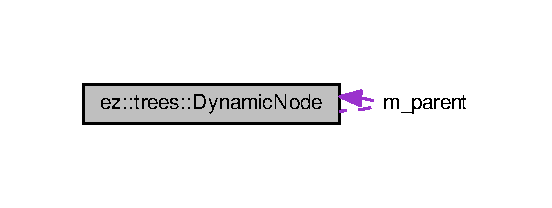
\includegraphics[width=265pt]{classez_1_1trees_1_1DynamicNode__coll__graph}
\end{center}
\end{figure}
\subsection*{Public Types}
\begin{DoxyCompactItemize}
\item 
\mbox{\Hypertarget{classez_1_1trees_1_1DynamicNode_aafafeeedfad803ab01c6a7eb5c5c0eb7}\label{classez_1_1trees_1_1DynamicNode_aafafeeedfad803ab01c6a7eb5c5c0eb7}} 
typedef \hyperlink{classez_1_1trees_1_1DynamicNode}{Dynamic\+Node} {\bfseries self}
\end{DoxyCompactItemize}
\subsection*{Public Member Functions}
\begin{DoxyCompactItemize}
\item 
\mbox{\Hypertarget{classez_1_1trees_1_1DynamicNode_a7ffc014663c9d4a612965fffa80945d6}\label{classez_1_1trees_1_1DynamicNode_a7ffc014663c9d4a612965fffa80945d6}} 
{\bfseries Dynamic\+Node} (const \hyperlink{classez_1_1trees_1_1DynamicNode}{Dynamic\+Node} \&obj)
\item 
\mbox{\Hypertarget{classez_1_1trees_1_1DynamicNode_ac22b2d1b0f2c1be60eff3a93e9960cc2}\label{classez_1_1trees_1_1DynamicNode_ac22b2d1b0f2c1be60eff3a93e9960cc2}} 
\hyperlink{classez_1_1trees_1_1DynamicNode}{Dynamic\+Node} \& {\bfseries operator=} (const \hyperlink{classez_1_1trees_1_1DynamicNode}{Dynamic\+Node} \&obj)
\item 
\mbox{\Hypertarget{classez_1_1trees_1_1DynamicNode_a9138f42ed8c80c175116567addaf868e}\label{classez_1_1trees_1_1DynamicNode_a9138f42ed8c80c175116567addaf868e}} 
\hyperlink{classez_1_1trees_1_1DynamicNode}{self} $\ast$ {\bfseries clone} ()
\item 
\mbox{\Hypertarget{classez_1_1trees_1_1DynamicNode_af1e7a0eeb6ac4df2f8a3a32b89139737}\label{classez_1_1trees_1_1DynamicNode_af1e7a0eeb6ac4df2f8a3a32b89139737}} 
void {\bfseries clean} ()
\item 
\mbox{\Hypertarget{classez_1_1trees_1_1DynamicNode_adca03f431f8d2582d7640db515bf6f71}\label{classez_1_1trees_1_1DynamicNode_adca03f431f8d2582d7640db515bf6f71}} 
bool {\bfseries is\+\_\+root} ()
\item 
\mbox{\Hypertarget{classez_1_1trees_1_1DynamicNode_ad6944cf15d216c20e9da8e5c031ea4f2}\label{classez_1_1trees_1_1DynamicNode_ad6944cf15d216c20e9da8e5c031ea4f2}} 
bool {\bfseries is\+\_\+leaf} ()
\item 
\mbox{\Hypertarget{classez_1_1trees_1_1DynamicNode_a3ec193dde9e1ed1eef9a02cf27ea16d5}\label{classez_1_1trees_1_1DynamicNode_a3ec193dde9e1ed1eef9a02cf27ea16d5}} 
\hyperlink{classez_1_1trees_1_1DynamicNode}{self} $\ast$ {\bfseries parent} ()
\item 
\mbox{\Hypertarget{classez_1_1trees_1_1DynamicNode_a30db00766456f8fc5db216cd5ffbd676}\label{classez_1_1trees_1_1DynamicNode_a30db00766456f8fc5db216cd5ffbd676}} 
void {\bfseries parent} (\hyperlink{classez_1_1trees_1_1DynamicNode}{self} $\ast$parent)
\item 
\mbox{\Hypertarget{classez_1_1trees_1_1DynamicNode_aacfcf4064fa5c878934fb56adb1358fb}\label{classez_1_1trees_1_1DynamicNode_aacfcf4064fa5c878934fb56adb1358fb}} 
void {\bfseries add} (\hyperlink{classez_1_1trees_1_1DynamicNode}{self} $\ast$node)
\item 
\mbox{\Hypertarget{classez_1_1trees_1_1DynamicNode_a6e406a29b3ada317a25e8a62a566a4d1}\label{classez_1_1trees_1_1DynamicNode_a6e406a29b3ada317a25e8a62a566a4d1}} 
\hyperlink{classez_1_1trees_1_1DynamicNode}{self} $\ast$ {\bfseries operator\mbox{[}$\,$\mbox{]}} (natural n)
\item 
\mbox{\Hypertarget{classez_1_1trees_1_1DynamicNode_a45bab83e51c44663e698c64e63907041}\label{classez_1_1trees_1_1DynamicNode_a45bab83e51c44663e698c64e63907041}} 
\hyperlink{classez_1_1trees_1_1DynamicNode}{self} $\ast$ {\bfseries replace} (natural position, \hyperlink{classez_1_1trees_1_1DynamicNode}{self} $\ast$node)
\item 
\mbox{\Hypertarget{classez_1_1trees_1_1DynamicNode_a7e7361a0e165b536330340f3b0222a54}\label{classez_1_1trees_1_1DynamicNode_a7e7361a0e165b536330340f3b0222a54}} 
\hyperlink{classez_1_1trees_1_1DynamicNode}{self} $\ast$ {\bfseries remove} (natural position)
\item 
\mbox{\Hypertarget{classez_1_1trees_1_1DynamicNode_a79b27d469d14b4d4c052c6b663563da7}\label{classez_1_1trees_1_1DynamicNode_a79b27d469d14b4d4c052c6b663563da7}} 
void {\bfseries print} (std\+::ostream \&out)
\item 
\mbox{\Hypertarget{classez_1_1trees_1_1DynamicNode_aa362b48c3499a959d3bd1ee030ca3c99}\label{classez_1_1trees_1_1DynamicNode_aa362b48c3499a959d3bd1ee030ca3c99}} 
void {\bfseries check} ()
\item 
\mbox{\Hypertarget{classez_1_1trees_1_1DynamicNode_aab4a7ef62acda0ee461b68be113091b4}\label{classez_1_1trees_1_1DynamicNode_aab4a7ef62acda0ee461b68be113091b4}} 
void {\bfseries internals} (vector$<$ \hyperlink{classez_1_1trees_1_1DynamicNode}{self} $\ast$$>$ \&v)
\item 
\mbox{\Hypertarget{classez_1_1trees_1_1DynamicNode_ad03ddbe0eaa30ce687ce79820e4282e0}\label{classez_1_1trees_1_1DynamicNode_ad03ddbe0eaa30ce687ce79820e4282e0}} 
void {\bfseries externals} (vector$<$ \hyperlink{classez_1_1trees_1_1DynamicNode}{self} $\ast$$>$ \&v)
\item 
\mbox{\Hypertarget{classez_1_1trees_1_1DynamicNode_ac4760bded5c71ac872c613dd3861c80c}\label{classez_1_1trees_1_1DynamicNode_ac4760bded5c71ac872c613dd3861c80c}} 
void {\bfseries all\+\_\+nodes} (vector$<$ \hyperlink{classez_1_1trees_1_1DynamicNode}{self} $\ast$$>$ \&v)
\end{DoxyCompactItemize}
\subsection*{Data Fields}
\begin{DoxyCompactItemize}
\item 
\mbox{\Hypertarget{classez_1_1trees_1_1DynamicNode_aa64bd46a4f52ee22e4e78dbfc08a1fb0}\label{classez_1_1trees_1_1DynamicNode_aa64bd46a4f52ee22e4e78dbfc08a1fb0}} 
std\+::vector$<$ \hyperlink{classez_1_1trees_1_1DynamicNode}{self} $\ast$ $>$ {\bfseries m\+\_\+nodes}
\item 
\mbox{\Hypertarget{classez_1_1trees_1_1DynamicNode_acef521e8514b8c7d3c5e6577e8766580}\label{classez_1_1trees_1_1DynamicNode_acef521e8514b8c7d3c5e6577e8766580}} 
\hyperlink{classez_1_1trees_1_1DynamicNode}{self} $\ast$ {\bfseries m\+\_\+parent}
\end{DoxyCompactItemize}
\subsection*{Friends}
\begin{DoxyCompactItemize}
\item 
\mbox{\Hypertarget{classez_1_1trees_1_1DynamicNode_aa1d826e7fbedbc2b2358e08bc03fc894}\label{classez_1_1trees_1_1DynamicNode_aa1d826e7fbedbc2b2358e08bc03fc894}} 
std\+::ostream \& {\bfseries operator$<$$<$} (std\+::ostream \&out, \hyperlink{classez_1_1trees_1_1DynamicNode}{self} \&obj)
\end{DoxyCompactItemize}


The documentation for this class was generated from the following files\+:\begin{DoxyCompactItemize}
\item 
src/version\+\_\+2018.\+06/trees/dynamic\+\_\+node.\+h\item 
src/version\+\_\+2018.\+06/trees/dynamic\+\_\+node.\+cpp\end{DoxyCompactItemize}

\hypertarget{classez_1_1trees_1_1DynamicTree}{}\section{ez\+:\+:trees\+:\+:Dynamic\+Tree Class Reference}
\label{classez_1_1trees_1_1DynamicTree}\index{ez\+::trees\+::\+Dynamic\+Tree@{ez\+::trees\+::\+Dynamic\+Tree}}


Inheritance diagram for ez\+:\+:trees\+:\+:Dynamic\+Tree\+:
\nopagebreak
\begin{figure}[H]
\begin{center}
\leavevmode
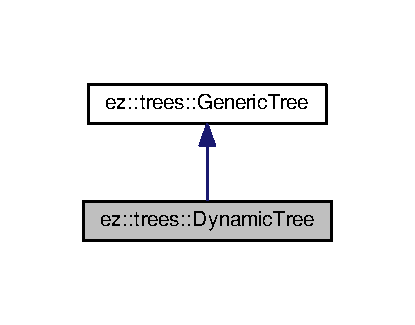
\includegraphics[width=199pt]{classez_1_1trees_1_1DynamicTree__inherit__graph}
\end{center}
\end{figure}


Collaboration diagram for ez\+:\+:trees\+:\+:Dynamic\+Tree\+:
\nopagebreak
\begin{figure}[H]
\begin{center}
\leavevmode
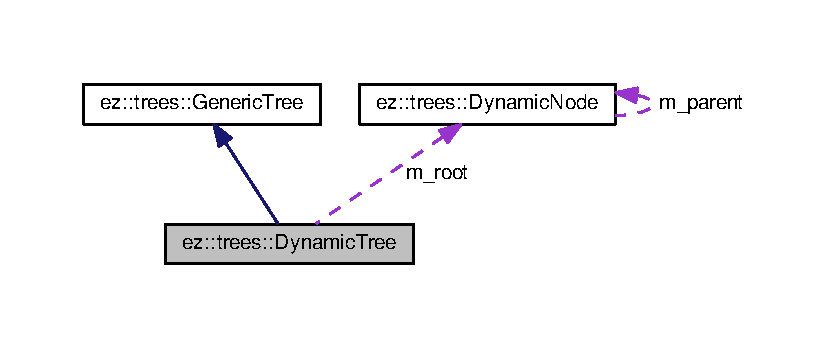
\includegraphics[width=350pt]{classez_1_1trees_1_1DynamicTree__coll__graph}
\end{center}
\end{figure}
\subsection*{Public Types}
\begin{DoxyCompactItemize}
\item 
\mbox{\Hypertarget{classez_1_1trees_1_1DynamicTree_a6c838c0e4a52ab62eafabcd98cd123dc}\label{classez_1_1trees_1_1DynamicTree_a6c838c0e4a52ab62eafabcd98cd123dc}} 
typedef \hyperlink{classez_1_1trees_1_1DynamicTree}{Dynamic\+Tree} {\bfseries self}
\item 
\mbox{\Hypertarget{classez_1_1trees_1_1DynamicTree_afb62febcd0e0b8ab3715fc706d24add7}\label{classez_1_1trees_1_1DynamicTree_afb62febcd0e0b8ab3715fc706d24add7}} 
typedef \hyperlink{classez_1_1trees_1_1DynamicNode}{Dynamic\+Node} $\ast$ {\bfseries Node}
\end{DoxyCompactItemize}
\subsection*{Public Member Functions}
\begin{DoxyCompactItemize}
\item 
\mbox{\Hypertarget{classez_1_1trees_1_1DynamicTree_a9b5a79a5db2c79cb753dcd73fad38fea}\label{classez_1_1trees_1_1DynamicTree_a9b5a79a5db2c79cb753dcd73fad38fea}} 
{\bfseries Dynamic\+Tree} (\hyperlink{classez_1_1trees_1_1DynamicNode}{Node} root)
\item 
\mbox{\Hypertarget{classez_1_1trees_1_1DynamicTree_a7c554953cab2445da03e5c768dbee461}\label{classez_1_1trees_1_1DynamicTree_a7c554953cab2445da03e5c768dbee461}} 
{\bfseries Dynamic\+Tree} (const \hyperlink{classez_1_1trees_1_1DynamicTree}{Dynamic\+Tree} \&obj)
\item 
\mbox{\Hypertarget{classez_1_1trees_1_1DynamicTree_a092f66c0070c7ec99088664ac2320b3b}\label{classez_1_1trees_1_1DynamicTree_a092f66c0070c7ec99088664ac2320b3b}} 
\hyperlink{classez_1_1trees_1_1DynamicTree}{Dynamic\+Tree} \& {\bfseries operator=} (const \hyperlink{classez_1_1trees_1_1DynamicTree}{Dynamic\+Tree} \&obj)
\item 
\mbox{\Hypertarget{classez_1_1trees_1_1DynamicTree_a2884268cbef7f33c3083074c94960c58}\label{classez_1_1trees_1_1DynamicTree_a2884268cbef7f33c3083074c94960c58}} 
\hyperlink{classez_1_1trees_1_1DynamicNode}{Node} {\bfseries root} (\hyperlink{classez_1_1trees_1_1DynamicNode}{Node} root)
\item 
\mbox{\Hypertarget{classez_1_1trees_1_1DynamicTree_a581921c9e8e066f3a369e3cc938688b4}\label{classez_1_1trees_1_1DynamicTree_a581921c9e8e066f3a369e3cc938688b4}} 
\hyperlink{classez_1_1trees_1_1DynamicTree}{Dynamic\+Tree} $\ast$ {\bfseries clone} ()
\item 
\mbox{\Hypertarget{classez_1_1trees_1_1DynamicTree_a000f6b52c2570e0823df719d60077b65}\label{classez_1_1trees_1_1DynamicTree_a000f6b52c2570e0823df719d60077b65}} 
void {\bfseries print} (std\+::ostream \&out)
\item 
\mbox{\Hypertarget{classez_1_1trees_1_1DynamicTree_a48602b01c5d440c0d935a7f691a02321}\label{classez_1_1trees_1_1DynamicTree_a48602b01c5d440c0d935a7f691a02321}} 
void {\bfseries check} ()
\item 
\mbox{\Hypertarget{classez_1_1trees_1_1DynamicTree_ad1346106fdd05be7ffd407b5e573057e}\label{classez_1_1trees_1_1DynamicTree_ad1346106fdd05be7ffd407b5e573057e}} 
void {\bfseries internals} (vector$<$ \hyperlink{classez_1_1trees_1_1DynamicNode}{Node} $>$ \&v)
\item 
\mbox{\Hypertarget{classez_1_1trees_1_1DynamicTree_afbdf8368cf4b8ba2665cfd1c6477addf}\label{classez_1_1trees_1_1DynamicTree_afbdf8368cf4b8ba2665cfd1c6477addf}} 
void {\bfseries externals} (vector$<$ \hyperlink{classez_1_1trees_1_1DynamicNode}{Node} $>$ \&v)
\item 
\mbox{\Hypertarget{classez_1_1trees_1_1DynamicTree_aadeda48b1ef2a83c9dee13961ea28ec2}\label{classez_1_1trees_1_1DynamicTree_aadeda48b1ef2a83c9dee13961ea28ec2}} 
void {\bfseries all\+\_\+nodes} (vector$<$ \hyperlink{classez_1_1trees_1_1DynamicNode}{Node} $>$ \&v)
\end{DoxyCompactItemize}
\subsection*{Data Fields}
\begin{DoxyCompactItemize}
\item 
\mbox{\Hypertarget{classez_1_1trees_1_1DynamicTree_aefa9c648dff841f4289f1991c6aa7673}\label{classez_1_1trees_1_1DynamicTree_aefa9c648dff841f4289f1991c6aa7673}} 
\hyperlink{classez_1_1trees_1_1DynamicNode}{Node} {\bfseries m\+\_\+root}
\end{DoxyCompactItemize}


The documentation for this class was generated from the following files\+:\begin{DoxyCompactItemize}
\item 
src/version\+\_\+2018.\+06/trees/dynamic\+\_\+tree.\+h\item 
src/version\+\_\+2018.\+06/trees/dynamic\+\_\+tree.\+cpp\end{DoxyCompactItemize}

\hypertarget{classez_1_1essential_1_1Exception}{}\section{ez\+:\+:essential\+:\+:Exception Class Reference}
\label{classez_1_1essential_1_1Exception}\index{ez\+::essential\+::\+Exception@{ez\+::essential\+::\+Exception}}


{\ttfamily \#include $<$exception.\+h$>$}



Inheritance diagram for ez\+:\+:essential\+:\+:Exception\+:
\nopagebreak
\begin{figure}[H]
\begin{center}
\leavevmode
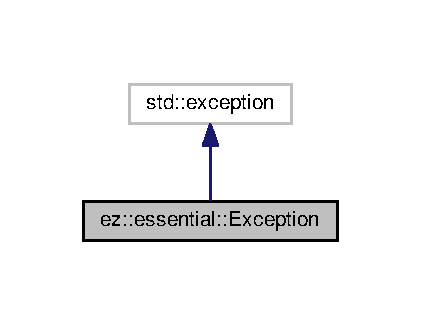
\includegraphics[width=202pt]{classez_1_1essential_1_1Exception__inherit__graph}
\end{center}
\end{figure}


Collaboration diagram for ez\+:\+:essential\+:\+:Exception\+:
\nopagebreak
\begin{figure}[H]
\begin{center}
\leavevmode
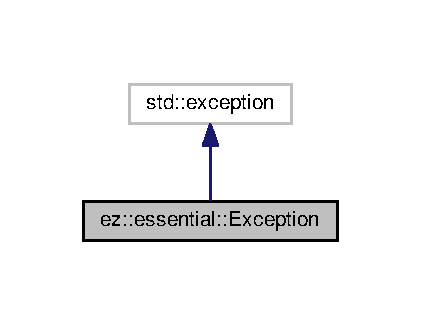
\includegraphics[width=202pt]{classez_1_1essential_1_1Exception__coll__graph}
\end{center}
\end{figure}
\subsection*{Public Member Functions}
\begin{DoxyCompactItemize}
\item 
\mbox{\Hypertarget{classez_1_1essential_1_1Exception_a0fd6d33274aa5d386399a1d35c65a640}\label{classez_1_1essential_1_1Exception_a0fd6d33274aa5d386399a1d35c65a640}} 
{\bfseries Exception} (const char $\ast$in\+\_\+file, integer at\+\_\+line)
\item 
const char $\ast$ \hyperlink{classez_1_1essential_1_1Exception_aa330aa854000f17a93919417d977bcac}{what} () const  throw ()
\item 
\mbox{\Hypertarget{classez_1_1essential_1_1Exception_a8352ffc60d214a4b9a5739fee37bc829}\label{classez_1_1essential_1_1Exception_a8352ffc60d214a4b9a5739fee37bc829}} 
void {\bfseries print\+\_\+stack\+\_\+trace} (std\+::ostream \&out)
\end{DoxyCompactItemize}
\subsection*{Static Public Member Functions}
\begin{DoxyCompactItemize}
\item 
\mbox{\Hypertarget{classez_1_1essential_1_1Exception_aedbe86bdf9456a597c6b9f11cde481fd}\label{classez_1_1essential_1_1Exception_aedbe86bdf9456a597c6b9f11cde481fd}} 
static void {\bfseries clear} ()
\end{DoxyCompactItemize}
\subsection*{Data Fields}
\begin{DoxyCompactItemize}
\item 
\mbox{\Hypertarget{classez_1_1essential_1_1Exception_aea83319eb701ca107bbfd3e5e3900840}\label{classez_1_1essential_1_1Exception_aea83319eb701ca107bbfd3e5e3900840}} 
const char $\ast$ {\bfseries m\+\_\+in\+\_\+file}
\item 
\mbox{\Hypertarget{classez_1_1essential_1_1Exception_a0d9fb7703923a5e5780429c9dd088592}\label{classez_1_1essential_1_1Exception_a0d9fb7703923a5e5780429c9dd088592}} 
integer {\bfseries m\+\_\+at\+\_\+line}
\end{DoxyCompactItemize}


\subsection{Detailed Description}
\hyperlink{classez_1_1essential_1_1Exception}{Exception} for the EZ Library We are using the cexc stream to give some message about the cause of the error and we record the file and line where it occured 

\subsection{Member Function Documentation}
\mbox{\Hypertarget{classez_1_1essential_1_1Exception_aa330aa854000f17a93919417d977bcac}\label{classez_1_1essential_1_1Exception_aa330aa854000f17a93919417d977bcac}} 
\index{ez\+::essential\+::\+Exception@{ez\+::essential\+::\+Exception}!what@{what}}
\index{what@{what}!ez\+::essential\+::\+Exception@{ez\+::essential\+::\+Exception}}
\subsubsection{\texorpdfstring{what()}{what()}}
{\footnotesize\ttfamily const char $\ast$ Exception\+::what (\begin{DoxyParamCaption}{ }\end{DoxyParamCaption}) const throw  ) }

return error message to print 

The documentation for this class was generated from the following files\+:\begin{DoxyCompactItemize}
\item 
src/version\+\_\+2018.\+06/essential/exception.\+h\item 
src/version\+\_\+2018.\+06/essential/exception.\+cpp\end{DoxyCompactItemize}

\hypertarget{classez_1_1logging_1_1FileLogger}{}\section{ez\+:\+:logging\+:\+:File\+Logger Class Reference}
\label{classez_1_1logging_1_1FileLogger}\index{ez\+::logging\+::\+File\+Logger@{ez\+::logging\+::\+File\+Logger}}


{\ttfamily \#include $<$logger.\+h$>$}



Inheritance diagram for ez\+:\+:logging\+:\+:File\+Logger\+:
\nopagebreak
\begin{figure}[H]
\begin{center}
\leavevmode
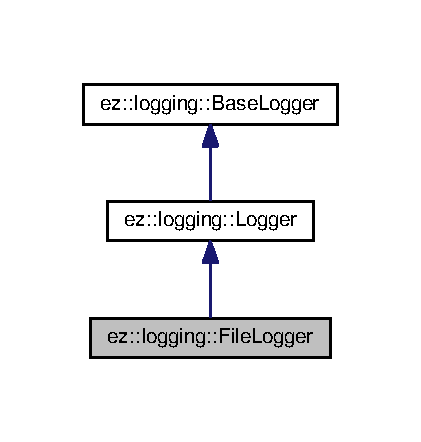
\includegraphics[width=202pt]{classez_1_1logging_1_1FileLogger__inherit__graph}
\end{center}
\end{figure}


Collaboration diagram for ez\+:\+:logging\+:\+:File\+Logger\+:
\nopagebreak
\begin{figure}[H]
\begin{center}
\leavevmode
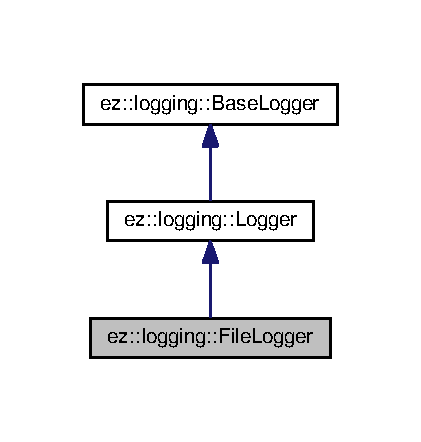
\includegraphics[width=202pt]{classez_1_1logging_1_1FileLogger__coll__graph}
\end{center}
\end{figure}
\subsection*{Public Member Functions}
\begin{DoxyCompactItemize}
\item 
\hyperlink{classez_1_1logging_1_1FileLogger_a5fdc65717e3a95b6ceb59a8c1b2943b5}{File\+Logger} (std\+::string name, std\+::string fn, integer options=0)
\item 
\hyperlink{classez_1_1logging_1_1FileLogger_ab08af44f2de3fe1b51158132f9a399dd}{$\sim$\+File\+Logger} ()
\end{DoxyCompactItemize}
\subsection*{Static Public Attributes}
\begin{DoxyCompactItemize}
\item 
\mbox{\Hypertarget{classez_1_1logging_1_1FileLogger_a0c9b0d3537b56031a895ee5aa942e0ad}\label{classez_1_1logging_1_1FileLogger_a0c9b0d3537b56031a895ee5aa942e0ad}} 
static const integer {\bfseries T\+R\+U\+N\+C\+A\+TE} = 1
\end{DoxyCompactItemize}
\subsection*{Protected Attributes}
\begin{DoxyCompactItemize}
\item 
\mbox{\Hypertarget{classez_1_1logging_1_1FileLogger_a499080349a0e13f132c66e713d96a826}\label{classez_1_1logging_1_1FileLogger_a499080349a0e13f132c66e713d96a826}} 
std\+::ofstream {\bfseries m\+\_\+stream}
\item 
\mbox{\Hypertarget{classez_1_1logging_1_1FileLogger_a15271eb566827586c5331adf2d71f179}\label{classez_1_1logging_1_1FileLogger_a15271eb566827586c5331adf2d71f179}} 
integer {\bfseries m\+\_\+options}
\end{DoxyCompactItemize}
\subsection*{Additional Inherited Members}


\subsection{Detailed Description}
\hyperlink{classez_1_1logging_1_1Logger}{Logger} that uses a file to store information 

\subsection{Constructor \& Destructor Documentation}
\mbox{\Hypertarget{classez_1_1logging_1_1FileLogger_a5fdc65717e3a95b6ceb59a8c1b2943b5}\label{classez_1_1logging_1_1FileLogger_a5fdc65717e3a95b6ceb59a8c1b2943b5}} 
\index{ez\+::logging\+::\+File\+Logger@{ez\+::logging\+::\+File\+Logger}!File\+Logger@{File\+Logger}}
\index{File\+Logger@{File\+Logger}!ez\+::logging\+::\+File\+Logger@{ez\+::logging\+::\+File\+Logger}}
\subsubsection{\texorpdfstring{File\+Logger()}{FileLogger()}}
{\footnotesize\ttfamily File\+Logger\+::\+File\+Logger (\begin{DoxyParamCaption}\item[{std\+::string}]{name,  }\item[{std\+::string}]{fn,  }\item[{integer}]{options = {\ttfamily 0} }\end{DoxyParamCaption})}

constructor 
\begin{DoxyParams}{Parameters}
{\em name} & identifier of logger \\
\hline
{\em fn} & file name \\
\hline
{\em opt} & options, for example T\+R\+U\+N\+C\+A\+TE will empty the file \\
\hline
\end{DoxyParams}
\mbox{\Hypertarget{classez_1_1logging_1_1FileLogger_ab08af44f2de3fe1b51158132f9a399dd}\label{classez_1_1logging_1_1FileLogger_ab08af44f2de3fe1b51158132f9a399dd}} 
\index{ez\+::logging\+::\+File\+Logger@{ez\+::logging\+::\+File\+Logger}!````~File\+Logger@{$\sim$\+File\+Logger}}
\index{````~File\+Logger@{$\sim$\+File\+Logger}!ez\+::logging\+::\+File\+Logger@{ez\+::logging\+::\+File\+Logger}}
\subsubsection{\texorpdfstring{$\sim$\+File\+Logger()}{~FileLogger()}}
{\footnotesize\ttfamily File\+Logger\+::$\sim$\+File\+Logger (\begin{DoxyParamCaption}{ }\end{DoxyParamCaption})}

destructor 

The documentation for this class was generated from the following files\+:\begin{DoxyCompactItemize}
\item 
src/version\+\_\+2018.\+06/logging/logger.\+h\item 
src/version\+\_\+2018.\+06/logging/logger.\+cpp\end{DoxyCompactItemize}

\hypertarget{classez_1_1arguments_1_1FlagArgument}{}\section{ez\+:\+:arguments\+:\+:Flag\+Argument Class Reference}
\label{classez_1_1arguments_1_1FlagArgument}\index{ez\+::arguments\+::\+Flag\+Argument@{ez\+::arguments\+::\+Flag\+Argument}}


{\ttfamily \#include $<$flag\+\_\+argument.\+h$>$}



Inheritance diagram for ez\+:\+:arguments\+:\+:Flag\+Argument\+:
\nopagebreak
\begin{figure}[H]
\begin{center}
\leavevmode
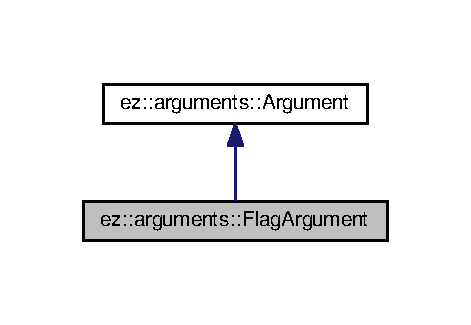
\includegraphics[width=226pt]{classez_1_1arguments_1_1FlagArgument__inherit__graph}
\end{center}
\end{figure}


Collaboration diagram for ez\+:\+:arguments\+:\+:Flag\+Argument\+:
\nopagebreak
\begin{figure}[H]
\begin{center}
\leavevmode
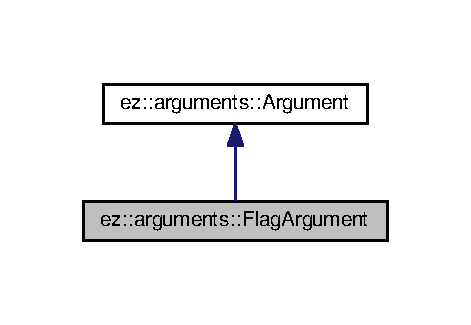
\includegraphics[width=226pt]{classez_1_1arguments_1_1FlagArgument__coll__graph}
\end{center}
\end{figure}
\subsection*{Public Member Functions}
\begin{DoxyCompactItemize}
\item 
\mbox{\Hypertarget{classez_1_1arguments_1_1FlagArgument_a30fffa2ded35d77bc527087a5ea13f81}\label{classez_1_1arguments_1_1FlagArgument_a30fffa2ded35d77bc527087a5ea13f81}} 
{\bfseries Flag\+Argument} (string long\+\_\+label, char short\+\_\+label, bool $\ast$value, string description, trigger\+\_\+t trigger=nullptr)
\item 
\mbox{\Hypertarget{classez_1_1arguments_1_1FlagArgument_a9d0fdf7d0981c5b49308d17f44b142c6}\label{classez_1_1arguments_1_1FlagArgument_a9d0fdf7d0981c5b49308d17f44b142c6}} 
void {\bfseries parse} (string \&s)
\end{DoxyCompactItemize}
\subsection*{Protected Attributes}
\begin{DoxyCompactItemize}
\item 
\mbox{\Hypertarget{classez_1_1arguments_1_1FlagArgument_ac93e0090f5854f573d90270b6d252eea}\label{classez_1_1arguments_1_1FlagArgument_ac93e0090f5854f573d90270b6d252eea}} 
bool $\ast$ {\bfseries m\+\_\+value}
\end{DoxyCompactItemize}


\subsection{Detailed Description}
class used to define flag argument that do not need any parameter or value like -\/v (verbose) 

The documentation for this class was generated from the following files\+:\begin{DoxyCompactItemize}
\item 
src/version\+\_\+2018.\+06/arguments/flag\+\_\+argument.\+h\item 
src/version\+\_\+2018.\+06/arguments/flag\+\_\+argument.\+cpp\end{DoxyCompactItemize}

\hypertarget{classez_1_1essential_1_1Format}{}\section{ez\+:\+:essential\+:\+:Format Class Reference}
\label{classez_1_1essential_1_1Format}\index{ez\+::essential\+::\+Format@{ez\+::essential\+::\+Format}}


{\ttfamily \#include $<$format.\+h$>$}

\subsection*{Static Public Member Functions}
\begin{DoxyCompactItemize}
\item 
static text \hyperlink{classez_1_1essential_1_1Format_ad77d7f94ad041e3905107c391dbcd00a}{left} (text s, integer width, character fill\+\_\+char=\textquotesingle{} \textquotesingle{})
\item 
static text \hyperlink{classez_1_1essential_1_1Format_aad619b944b2ab388ccb82b1d82ef610b}{center} (text s, integer width, character fill\+\_\+char=\textquotesingle{} \textquotesingle{})
\item 
static text \hyperlink{classez_1_1essential_1_1Format_a46180d9a7dd6202fb5225b1fe83f50bb}{right} (text s, integer width, character fill\+\_\+char=\textquotesingle{} \textquotesingle{})
\item 
static text \hyperlink{classez_1_1essential_1_1Format_ab163df0d05d66c0402c46ecfae2dee82}{dec} (long\+\_\+natural n)
\item 
static text \hyperlink{classez_1_1essential_1_1Format_a9fe91dede9e02e992d4ab410d89a0e21}{bin} (long\+\_\+natural n, natural size\+\_\+in\+\_\+bits=32)
\item 
static text \hyperlink{classez_1_1essential_1_1Format_ac5e90b9408d5ff10bbdf4cc0d4f55895}{oct} (long\+\_\+natural n)
\item 
static text \hyperlink{classez_1_1essential_1_1Format_aa61095f58c70d7a4dfcb1e555fd3673d}{hex} (long\+\_\+natural n)
\item 
\mbox{\Hypertarget{classez_1_1essential_1_1Format_a3afc25d1fc2e5085caaa56f64b6747b5}\label{classez_1_1essential_1_1Format_a3afc25d1fc2e5085caaa56f64b6747b5}} 
static text {\bfseries flt} (real n, natural size=0, natural decimals=0)
\end{DoxyCompactItemize}
\subsection*{Static Protected Member Functions}
\begin{DoxyCompactItemize}
\item 
\mbox{\Hypertarget{classez_1_1essential_1_1Format_abd388160f737b12027656a9a6328e7c0}\label{classez_1_1essential_1_1Format_abd388160f737b12027656a9a6328e7c0}} 
static text {\bfseries \+\_\+to\+\_\+base} (natural n, \hyperlink{classez_1_1essential_1_1NumericBase}{Numeric\+Base} \&base)
\item 
\mbox{\Hypertarget{classez_1_1essential_1_1Format_aed6b5776c9c040d952d7a4058fa0a51d}\label{classez_1_1essential_1_1Format_aed6b5776c9c040d952d7a4058fa0a51d}} 
static text {\bfseries \+\_\+to\+\_\+base} (long\+\_\+natural n, \hyperlink{classez_1_1essential_1_1NumericBase}{Numeric\+Base} \&base)
\item 
\mbox{\Hypertarget{classez_1_1essential_1_1Format_a243e4d7ade39eaf54436b198b67b1243}\label{classez_1_1essential_1_1Format_a243e4d7ade39eaf54436b198b67b1243}} 
static text {\bfseries \+\_\+format} (text s, integer distance)
\end{DoxyCompactItemize}


\subsection{Detailed Description}
\hyperlink{classez_1_1essential_1_1Format}{Format} to pretty print data 

\subsection{Member Function Documentation}
\mbox{\Hypertarget{classez_1_1essential_1_1Format_a9fe91dede9e02e992d4ab410d89a0e21}\label{classez_1_1essential_1_1Format_a9fe91dede9e02e992d4ab410d89a0e21}} 
\index{ez\+::essential\+::\+Format@{ez\+::essential\+::\+Format}!bin@{bin}}
\index{bin@{bin}!ez\+::essential\+::\+Format@{ez\+::essential\+::\+Format}}
\subsubsection{\texorpdfstring{bin()}{bin()}}
{\footnotesize\ttfamily text Format\+::bin (\begin{DoxyParamCaption}\item[{long\+\_\+natural}]{n,  }\item[{natural}]{size\+\_\+in\+\_\+bits = {\ttfamily 32} }\end{DoxyParamCaption})\hspace{0.3cm}{\ttfamily [static]}}

convert natural number to binary format \mbox{\Hypertarget{classez_1_1essential_1_1Format_aad619b944b2ab388ccb82b1d82ef610b}\label{classez_1_1essential_1_1Format_aad619b944b2ab388ccb82b1d82ef610b}} 
\index{ez\+::essential\+::\+Format@{ez\+::essential\+::\+Format}!center@{center}}
\index{center@{center}!ez\+::essential\+::\+Format@{ez\+::essential\+::\+Format}}
\subsubsection{\texorpdfstring{center()}{center()}}
{\footnotesize\ttfamily text Format\+::center (\begin{DoxyParamCaption}\item[{text}]{s,  }\item[{integer}]{width,  }\item[{character}]{fill\+\_\+char = {\ttfamily \textquotesingle{}~\textquotesingle{}} }\end{DoxyParamCaption})\hspace{0.3cm}{\ttfamily [static]}}

Print a string on the center of a given width and will with spaces \mbox{\Hypertarget{classez_1_1essential_1_1Format_ab163df0d05d66c0402c46ecfae2dee82}\label{classez_1_1essential_1_1Format_ab163df0d05d66c0402c46ecfae2dee82}} 
\index{ez\+::essential\+::\+Format@{ez\+::essential\+::\+Format}!dec@{dec}}
\index{dec@{dec}!ez\+::essential\+::\+Format@{ez\+::essential\+::\+Format}}
\subsubsection{\texorpdfstring{dec()}{dec()}}
{\footnotesize\ttfamily text Format\+::dec (\begin{DoxyParamCaption}\item[{long\+\_\+natural}]{n }\end{DoxyParamCaption})\hspace{0.3cm}{\ttfamily [static]}}

convert to decimal format \mbox{\Hypertarget{classez_1_1essential_1_1Format_aa61095f58c70d7a4dfcb1e555fd3673d}\label{classez_1_1essential_1_1Format_aa61095f58c70d7a4dfcb1e555fd3673d}} 
\index{ez\+::essential\+::\+Format@{ez\+::essential\+::\+Format}!hex@{hex}}
\index{hex@{hex}!ez\+::essential\+::\+Format@{ez\+::essential\+::\+Format}}
\subsubsection{\texorpdfstring{hex()}{hex()}}
{\footnotesize\ttfamily text Format\+::hex (\begin{DoxyParamCaption}\item[{long\+\_\+natural}]{n }\end{DoxyParamCaption})\hspace{0.3cm}{\ttfamily [static]}}

convert natural number to hexadecimal format \mbox{\Hypertarget{classez_1_1essential_1_1Format_ad77d7f94ad041e3905107c391dbcd00a}\label{classez_1_1essential_1_1Format_ad77d7f94ad041e3905107c391dbcd00a}} 
\index{ez\+::essential\+::\+Format@{ez\+::essential\+::\+Format}!left@{left}}
\index{left@{left}!ez\+::essential\+::\+Format@{ez\+::essential\+::\+Format}}
\subsubsection{\texorpdfstring{left()}{left()}}
{\footnotesize\ttfamily text Format\+::left (\begin{DoxyParamCaption}\item[{text}]{s,  }\item[{integer}]{width,  }\item[{character}]{fill\+\_\+char = {\ttfamily \textquotesingle{}~\textquotesingle{}} }\end{DoxyParamCaption})\hspace{0.3cm}{\ttfamily [static]}}

Print a string on the left of a given width and will with spaces 
\begin{DoxyParams}{Parameters}
{\em s} & string to print \\
\hline
{\em width} & \\
\hline
{\em fill\+\_\+char} & character to use to fill rest of the width \\
\hline
\end{DoxyParams}
\mbox{\Hypertarget{classez_1_1essential_1_1Format_ac5e90b9408d5ff10bbdf4cc0d4f55895}\label{classez_1_1essential_1_1Format_ac5e90b9408d5ff10bbdf4cc0d4f55895}} 
\index{ez\+::essential\+::\+Format@{ez\+::essential\+::\+Format}!oct@{oct}}
\index{oct@{oct}!ez\+::essential\+::\+Format@{ez\+::essential\+::\+Format}}
\subsubsection{\texorpdfstring{oct()}{oct()}}
{\footnotesize\ttfamily text Format\+::oct (\begin{DoxyParamCaption}\item[{long\+\_\+natural}]{n }\end{DoxyParamCaption})\hspace{0.3cm}{\ttfamily [static]}}

convert natural number to octal format \mbox{\Hypertarget{classez_1_1essential_1_1Format_a46180d9a7dd6202fb5225b1fe83f50bb}\label{classez_1_1essential_1_1Format_a46180d9a7dd6202fb5225b1fe83f50bb}} 
\index{ez\+::essential\+::\+Format@{ez\+::essential\+::\+Format}!right@{right}}
\index{right@{right}!ez\+::essential\+::\+Format@{ez\+::essential\+::\+Format}}
\subsubsection{\texorpdfstring{right()}{right()}}
{\footnotesize\ttfamily text Format\+::right (\begin{DoxyParamCaption}\item[{text}]{s,  }\item[{integer}]{width,  }\item[{character}]{fill\+\_\+char = {\ttfamily \textquotesingle{}~\textquotesingle{}} }\end{DoxyParamCaption})\hspace{0.3cm}{\ttfamily [static]}}

Print a string on the right of a given width and will with spaces 

The documentation for this class was generated from the following files\+:\begin{DoxyCompactItemize}
\item 
src/version\+\_\+2018.\+06/essential/format.\+h\item 
src/version\+\_\+2018.\+06/essential/format.\+cpp\end{DoxyCompactItemize}

\hypertarget{classez_1_1maths_1_1Frequency}{}\section{ez\+:\+:maths\+:\+:Frequency$<$ T $>$ Class Template Reference}
\label{classez_1_1maths_1_1Frequency}\index{ez\+::maths\+::\+Frequency$<$ T $>$@{ez\+::maths\+::\+Frequency$<$ T $>$}}


{\ttfamily \#include $<$frequency.\+h$>$}

\subsection*{Public Member Functions}
\begin{DoxyCompactItemize}
\item 
\hyperlink{classez_1_1maths_1_1Frequency_aa090ee7e4117d4f5a694de71c44ec789}{Frequency} ()
\item 
\hyperlink{classez_1_1maths_1_1Frequency_a5fe6cf61394f7fc424c4d93392f734a2}{Frequency} (T mini, T maxi, T incr, T delta=1)
\item 
void \hyperlink{classez_1_1maths_1_1Frequency_a93882872b801cb8f47e61f32b24a051a}{insert} (\hyperlink{classez_1_1maths_1_1Interval}{Interval}$<$ T $>$ c)
\item 
void \hyperlink{classez_1_1maths_1_1Frequency_acd474d72e33becac99dc5dff9bcdb3e8}{record} (T value)
\item 
real \hyperlink{classez_1_1maths_1_1Frequency_aa18480ae307a14ad3a528476194d022e}{total} ()
\item 
void \hyperlink{classez_1_1maths_1_1Frequency_a102cd5f7b102ee433126fe809b2dfccb}{store} (ostream \&out)
\item 
void \hyperlink{classez_1_1maths_1_1Frequency_a4b1bc9f927a526e0ca1bbc59f1a14ca6}{percentage} ()
\item 
void \hyperlink{classez_1_1maths_1_1Frequency_af24be0f62175280c79ef1107f4a07b8d}{export\+\_\+as\+\_\+series} (ostream \&out)
\end{DoxyCompactItemize}
\subsection*{Protected Types}
\begin{DoxyCompactItemize}
\item 
\mbox{\Hypertarget{classez_1_1maths_1_1Frequency_aa22594e9d41c897c4aec8c8527046e17}\label{classez_1_1maths_1_1Frequency_aa22594e9d41c897c4aec8c8527046e17}} 
typedef pair$<$ \hyperlink{classez_1_1maths_1_1Interval}{Interval}$<$ T $>$, real $>$ {\bfseries Element}
\end{DoxyCompactItemize}
\subsection*{Protected Attributes}
\begin{DoxyCompactItemize}
\item 
\mbox{\Hypertarget{classez_1_1maths_1_1Frequency_a0b35037580b2a5c38012f53f95f01500}\label{classez_1_1maths_1_1Frequency_a0b35037580b2a5c38012f53f95f01500}} 
vector$<$ Element $>$ {\bfseries m\+\_\+classes}
\end{DoxyCompactItemize}
\subsection*{Friends}
\begin{DoxyCompactItemize}
\item 
ostream \& \hyperlink{classez_1_1maths_1_1Frequency_a0909af66272f86930b70857efb6c6a7e}{operator$<$$<$} (ostream \&out, \hyperlink{classez_1_1maths_1_1Frequency}{Frequency}$<$ T $>$ \&obj)
\end{DoxyCompactItemize}


\subsection{Detailed Description}
\subsubsection*{template$<$class T$>$\newline
class ez\+::maths\+::\+Frequency$<$ T $>$}

this class counts the number of occurrences of some values in terms of classes 

\subsection{Constructor \& Destructor Documentation}
\mbox{\Hypertarget{classez_1_1maths_1_1Frequency_aa090ee7e4117d4f5a694de71c44ec789}\label{classez_1_1maths_1_1Frequency_aa090ee7e4117d4f5a694de71c44ec789}} 
\index{ez\+::maths\+::\+Frequency@{ez\+::maths\+::\+Frequency}!Frequency@{Frequency}}
\index{Frequency@{Frequency}!ez\+::maths\+::\+Frequency@{ez\+::maths\+::\+Frequency}}
\subsubsection{\texorpdfstring{Frequency()}{Frequency()}\hspace{0.1cm}{\footnotesize\ttfamily [1/2]}}
{\footnotesize\ttfamily template$<$class T $>$ \\
\hyperlink{classez_1_1maths_1_1Frequency}{ez\+::maths\+::\+Frequency}$<$ T $>$\+::\hyperlink{classez_1_1maths_1_1Frequency}{Frequency} (\begin{DoxyParamCaption}{ }\end{DoxyParamCaption})\hspace{0.3cm}{\ttfamily [inline]}}

default constructor \mbox{\Hypertarget{classez_1_1maths_1_1Frequency_a5fe6cf61394f7fc424c4d93392f734a2}\label{classez_1_1maths_1_1Frequency_a5fe6cf61394f7fc424c4d93392f734a2}} 
\index{ez\+::maths\+::\+Frequency@{ez\+::maths\+::\+Frequency}!Frequency@{Frequency}}
\index{Frequency@{Frequency}!ez\+::maths\+::\+Frequency@{ez\+::maths\+::\+Frequency}}
\subsubsection{\texorpdfstring{Frequency()}{Frequency()}\hspace{0.1cm}{\footnotesize\ttfamily [2/2]}}
{\footnotesize\ttfamily template$<$class T $>$ \\
\hyperlink{classez_1_1maths_1_1Frequency}{ez\+::maths\+::\+Frequency}$<$ T $>$\+::\hyperlink{classez_1_1maths_1_1Frequency}{Frequency} (\begin{DoxyParamCaption}\item[{T}]{mini,  }\item[{T}]{maxi,  }\item[{T}]{incr,  }\item[{T}]{delta = {\ttfamily 1} }\end{DoxyParamCaption})\hspace{0.3cm}{\ttfamily [inline]}}

constructor that generates classes 

\subsection{Member Function Documentation}
\mbox{\Hypertarget{classez_1_1maths_1_1Frequency_af24be0f62175280c79ef1107f4a07b8d}\label{classez_1_1maths_1_1Frequency_af24be0f62175280c79ef1107f4a07b8d}} 
\index{ez\+::maths\+::\+Frequency@{ez\+::maths\+::\+Frequency}!export\+\_\+as\+\_\+series@{export\+\_\+as\+\_\+series}}
\index{export\+\_\+as\+\_\+series@{export\+\_\+as\+\_\+series}!ez\+::maths\+::\+Frequency@{ez\+::maths\+::\+Frequency}}
\subsubsection{\texorpdfstring{export\+\_\+as\+\_\+series()}{export\_as\_series()}}
{\footnotesize\ttfamily template$<$class T $>$ \\
void \hyperlink{classez_1_1maths_1_1Frequency}{ez\+::maths\+::\+Frequency}$<$ T $>$\+::export\+\_\+as\+\_\+series (\begin{DoxyParamCaption}\item[{ostream \&}]{out }\end{DoxyParamCaption})\hspace{0.3cm}{\ttfamily [inline]}}

export as series for highcharts \mbox{\Hypertarget{classez_1_1maths_1_1Frequency_a93882872b801cb8f47e61f32b24a051a}\label{classez_1_1maths_1_1Frequency_a93882872b801cb8f47e61f32b24a051a}} 
\index{ez\+::maths\+::\+Frequency@{ez\+::maths\+::\+Frequency}!insert@{insert}}
\index{insert@{insert}!ez\+::maths\+::\+Frequency@{ez\+::maths\+::\+Frequency}}
\subsubsection{\texorpdfstring{insert()}{insert()}}
{\footnotesize\ttfamily template$<$class T $>$ \\
void \hyperlink{classez_1_1maths_1_1Frequency}{ez\+::maths\+::\+Frequency}$<$ T $>$\+::insert (\begin{DoxyParamCaption}\item[{\hyperlink{classez_1_1maths_1_1Interval}{Interval}$<$ T $>$}]{c }\end{DoxyParamCaption})\hspace{0.3cm}{\ttfamily [inline]}}

insert interval of values \mbox{\Hypertarget{classez_1_1maths_1_1Frequency_a4b1bc9f927a526e0ca1bbc59f1a14ca6}\label{classez_1_1maths_1_1Frequency_a4b1bc9f927a526e0ca1bbc59f1a14ca6}} 
\index{ez\+::maths\+::\+Frequency@{ez\+::maths\+::\+Frequency}!percentage@{percentage}}
\index{percentage@{percentage}!ez\+::maths\+::\+Frequency@{ez\+::maths\+::\+Frequency}}
\subsubsection{\texorpdfstring{percentage()}{percentage()}}
{\footnotesize\ttfamily template$<$class T $>$ \\
void \hyperlink{classez_1_1maths_1_1Frequency}{ez\+::maths\+::\+Frequency}$<$ T $>$\+::percentage (\begin{DoxyParamCaption}{ }\end{DoxyParamCaption})\hspace{0.3cm}{\ttfamily [inline]}}

convert frequencies to percentages \mbox{\Hypertarget{classez_1_1maths_1_1Frequency_acd474d72e33becac99dc5dff9bcdb3e8}\label{classez_1_1maths_1_1Frequency_acd474d72e33becac99dc5dff9bcdb3e8}} 
\index{ez\+::maths\+::\+Frequency@{ez\+::maths\+::\+Frequency}!record@{record}}
\index{record@{record}!ez\+::maths\+::\+Frequency@{ez\+::maths\+::\+Frequency}}
\subsubsection{\texorpdfstring{record()}{record()}}
{\footnotesize\ttfamily template$<$class T $>$ \\
void \hyperlink{classez_1_1maths_1_1Frequency}{ez\+::maths\+::\+Frequency}$<$ T $>$\+::record (\begin{DoxyParamCaption}\item[{T}]{value }\end{DoxyParamCaption})\hspace{0.3cm}{\ttfamily [inline]}}

record value \mbox{\Hypertarget{classez_1_1maths_1_1Frequency_a102cd5f7b102ee433126fe809b2dfccb}\label{classez_1_1maths_1_1Frequency_a102cd5f7b102ee433126fe809b2dfccb}} 
\index{ez\+::maths\+::\+Frequency@{ez\+::maths\+::\+Frequency}!store@{store}}
\index{store@{store}!ez\+::maths\+::\+Frequency@{ez\+::maths\+::\+Frequency}}
\subsubsection{\texorpdfstring{store()}{store()}}
{\footnotesize\ttfamily template$<$class T $>$ \\
void \hyperlink{classez_1_1maths_1_1Frequency}{ez\+::maths\+::\+Frequency}$<$ T $>$\+::store (\begin{DoxyParamCaption}\item[{ostream \&}]{out }\end{DoxyParamCaption})\hspace{0.3cm}{\ttfamily [inline]}}

store data to be used by gnuplot \mbox{\Hypertarget{classez_1_1maths_1_1Frequency_aa18480ae307a14ad3a528476194d022e}\label{classez_1_1maths_1_1Frequency_aa18480ae307a14ad3a528476194d022e}} 
\index{ez\+::maths\+::\+Frequency@{ez\+::maths\+::\+Frequency}!total@{total}}
\index{total@{total}!ez\+::maths\+::\+Frequency@{ez\+::maths\+::\+Frequency}}
\subsubsection{\texorpdfstring{total()}{total()}}
{\footnotesize\ttfamily template$<$class T $>$ \\
real \hyperlink{classez_1_1maths_1_1Frequency}{ez\+::maths\+::\+Frequency}$<$ T $>$\+::total (\begin{DoxyParamCaption}{ }\end{DoxyParamCaption})\hspace{0.3cm}{\ttfamily [inline]}}

record total number of values recorded 

\subsection{Friends And Related Function Documentation}
\mbox{\Hypertarget{classez_1_1maths_1_1Frequency_a0909af66272f86930b70857efb6c6a7e}\label{classez_1_1maths_1_1Frequency_a0909af66272f86930b70857efb6c6a7e}} 
\index{ez\+::maths\+::\+Frequency@{ez\+::maths\+::\+Frequency}!operator$<$$<$@{operator$<$$<$}}
\index{operator$<$$<$@{operator$<$$<$}!ez\+::maths\+::\+Frequency@{ez\+::maths\+::\+Frequency}}
\subsubsection{\texorpdfstring{operator$<$$<$}{operator<<}}
{\footnotesize\ttfamily template$<$class T $>$ \\
ostream\& operator$<$$<$ (\begin{DoxyParamCaption}\item[{ostream \&}]{out,  }\item[{\hyperlink{classez_1_1maths_1_1Frequency}{Frequency}$<$ T $>$ \&}]{obj }\end{DoxyParamCaption})\hspace{0.3cm}{\ttfamily [friend]}}

overloading of output operator 

The documentation for this class was generated from the following file\+:\begin{DoxyCompactItemize}
\item 
src/version\+\_\+2018.\+06/maths/frequency.\+h\end{DoxyCompactItemize}

\hypertarget{classez_1_1extensions_1_1Generator}{}\section{ez\+:\+:extensions\+:\+:Generator$<$ Data\+Type $>$ Class Template Reference}
\label{classez_1_1extensions_1_1Generator}\index{ez\+::extensions\+::\+Generator$<$ Data\+Type $>$@{ez\+::extensions\+::\+Generator$<$ Data\+Type $>$}}
\subsection*{Public Member Functions}
\begin{DoxyCompactItemize}
\item 
\mbox{\Hypertarget{classez_1_1extensions_1_1Generator_aa1ad45d137f72ca49ad106ce802f6879}\label{classez_1_1extensions_1_1Generator_aa1ad45d137f72ca49ad106ce802f6879}} 
{\bfseries Generator} (Data\+Type initial=1, Data\+Type increment=1)
\item 
\mbox{\Hypertarget{classez_1_1extensions_1_1Generator_af462de2c0915a4c808a679872973e722}\label{classez_1_1extensions_1_1Generator_af462de2c0915a4c808a679872973e722}} 
Data\+Type {\bfseries operator()} ()
\end{DoxyCompactItemize}
\subsection*{Data Fields}
\begin{DoxyCompactItemize}
\item 
\mbox{\Hypertarget{classez_1_1extensions_1_1Generator_a9926ada804b51a3ea78804f05f8ad25a}\label{classez_1_1extensions_1_1Generator_a9926ada804b51a3ea78804f05f8ad25a}} 
Data\+Type {\bfseries m\+\_\+initial}
\item 
\mbox{\Hypertarget{classez_1_1extensions_1_1Generator_aa4887f0e6a0d77671239d665fde9d4df}\label{classez_1_1extensions_1_1Generator_aa4887f0e6a0d77671239d665fde9d4df}} 
Data\+Type {\bfseries m\+\_\+increment}
\end{DoxyCompactItemize}


The documentation for this class was generated from the following file\+:\begin{DoxyCompactItemize}
\item 
src/version\+\_\+2018.\+06/extensions/generator.\+h\end{DoxyCompactItemize}

\hypertarget{classez_1_1trees_1_1GenericTree}{}\section{ez\+:\+:trees\+:\+:Generic\+Tree Class Reference}
\label{classez_1_1trees_1_1GenericTree}\index{ez\+::trees\+::\+Generic\+Tree@{ez\+::trees\+::\+Generic\+Tree}}


Inheritance diagram for ez\+:\+:trees\+:\+:Generic\+Tree\+:
\nopagebreak
\begin{figure}[H]
\begin{center}
\leavevmode
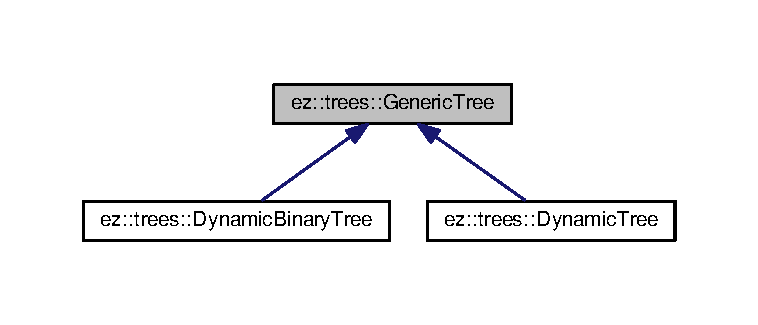
\includegraphics[width=350pt]{classez_1_1trees_1_1GenericTree__inherit__graph}
\end{center}
\end{figure}
\subsection*{Public Member Functions}
\begin{DoxyCompactItemize}
\item 
\mbox{\Hypertarget{classez_1_1trees_1_1GenericTree_a592c6880012b7eea9d5d982b9801ee79}\label{classez_1_1trees_1_1GenericTree_a592c6880012b7eea9d5d982b9801ee79}} 
virtual void {\bfseries print} (std\+::ostream \&out)=0
\end{DoxyCompactItemize}
\subsection*{Friends}
\begin{DoxyCompactItemize}
\item 
\mbox{\Hypertarget{classez_1_1trees_1_1GenericTree_a325057120eaf73f31376e04f3d6ece45}\label{classez_1_1trees_1_1GenericTree_a325057120eaf73f31376e04f3d6ece45}} 
std\+::ostream \& {\bfseries operator$<$$<$} (std\+::ostream \&out, \hyperlink{classez_1_1trees_1_1DynamicTree}{Dynamic\+Tree} \&obj)
\end{DoxyCompactItemize}


The documentation for this class was generated from the following file\+:\begin{DoxyCompactItemize}
\item 
src/version\+\_\+2018.\+06/trees/generic\+\_\+tree.\+h\end{DoxyCompactItemize}

\hypertarget{classez_1_1maths_1_1Geometry2D}{}\section{ez\+:\+:maths\+:\+:Geometry2D Class Reference}
\label{classez_1_1maths_1_1Geometry2D}\index{ez\+::maths\+::\+Geometry2D@{ez\+::maths\+::\+Geometry2D}}
\subsection*{Public Types}
\begin{DoxyCompactItemize}
\item 
\mbox{\Hypertarget{classez_1_1maths_1_1Geometry2D_a686fb50d9c63b622916b7f3faab0c620}\label{classez_1_1maths_1_1Geometry2D_a686fb50d9c63b622916b7f3faab0c620}} 
typedef \hyperlink{classez_1_1maths_1_1Matrix}{ez\+::maths\+::\+Matrix}$<$ long\+\_\+real $>$ {\bfseries Long\+Real\+Matrix}
\end{DoxyCompactItemize}
\subsection*{Static Public Member Functions}
\begin{DoxyCompactItemize}
\item 
\mbox{\Hypertarget{classez_1_1maths_1_1Geometry2D_a495e445c642152ab2ad4d8a6aaec3f09}\label{classez_1_1maths_1_1Geometry2D_a495e445c642152ab2ad4d8a6aaec3f09}} 
static void {\bfseries matrix\+\_\+rotate} (real angle\+\_\+in\+\_\+degrees, \hyperlink{classez_1_1maths_1_1Matrix}{Long\+Real\+Matrix} \&matrix)
\item 
\mbox{\Hypertarget{classez_1_1maths_1_1Geometry2D_a23fcbdff26104254e2085788950c87b8}\label{classez_1_1maths_1_1Geometry2D_a23fcbdff26104254e2085788950c87b8}} 
static void {\bfseries product} (\hyperlink{classez_1_1maths_1_1Point2D}{Point2D} \&r, \hyperlink{classez_1_1maths_1_1Matrix}{Long\+Real\+Matrix} \&m, \hyperlink{classez_1_1maths_1_1Point2D}{Point2D} \&v)
\end{DoxyCompactItemize}


The documentation for this class was generated from the following files\+:\begin{DoxyCompactItemize}
\item 
src/version\+\_\+2018.\+06/maths/geometry2d.\+h\item 
src/version\+\_\+2018.\+06/maths/geometry2d.\+cpp\end{DoxyCompactItemize}

\hypertarget{classez_1_1maths_1_1Geometry3D}{}\section{ez\+:\+:maths\+:\+:Geometry3D Class Reference}
\label{classez_1_1maths_1_1Geometry3D}\index{ez\+::maths\+::\+Geometry3D@{ez\+::maths\+::\+Geometry3D}}
\subsection*{Public Types}
\begin{DoxyCompactItemize}
\item 
\mbox{\Hypertarget{classez_1_1maths_1_1Geometry3D_a6fd780ac0cf0a374c4ce5ba672124e47}\label{classez_1_1maths_1_1Geometry3D_a6fd780ac0cf0a374c4ce5ba672124e47}} 
typedef \hyperlink{classez_1_1maths_1_1Matrix}{ez\+::maths\+::\+Matrix}$<$ long\+\_\+real $>$ {\bfseries G\+Matrix}
\end{DoxyCompactItemize}
\subsection*{Static Public Member Functions}
\begin{DoxyCompactItemize}
\item 
\mbox{\Hypertarget{classez_1_1maths_1_1Geometry3D_a984d41dccfd8ae531dd1f881b1b871d4}\label{classez_1_1maths_1_1Geometry3D_a984d41dccfd8ae531dd1f881b1b871d4}} 
static void {\bfseries matrix\+\_\+rotate\+\_\+x} (real angle\+\_\+in\+\_\+degrees, \hyperlink{classez_1_1maths_1_1Matrix}{G\+Matrix} \&matrix)
\item 
\mbox{\Hypertarget{classez_1_1maths_1_1Geometry3D_aba5c04e727d4037805a1ba49fcd31c74}\label{classez_1_1maths_1_1Geometry3D_aba5c04e727d4037805a1ba49fcd31c74}} 
static void {\bfseries matrix\+\_\+rotate\+\_\+y} (real angle\+\_\+in\+\_\+degrees, \hyperlink{classez_1_1maths_1_1Matrix}{G\+Matrix} \&matrix)
\item 
\mbox{\Hypertarget{classez_1_1maths_1_1Geometry3D_afec5eb63f2cad9405ad2a1ed1a61a888}\label{classez_1_1maths_1_1Geometry3D_afec5eb63f2cad9405ad2a1ed1a61a888}} 
static void {\bfseries matrix\+\_\+rotate\+\_\+z} (real angle\+\_\+in\+\_\+degrees, \hyperlink{classez_1_1maths_1_1Matrix}{G\+Matrix} \&matrix)
\item 
\mbox{\Hypertarget{classez_1_1maths_1_1Geometry3D_a086bb92115126299f7ac74af0e7363a6}\label{classez_1_1maths_1_1Geometry3D_a086bb92115126299f7ac74af0e7363a6}} 
static void {\bfseries product} (\hyperlink{classez_1_1maths_1_1Point3D}{Point3D} \&r, \hyperlink{classez_1_1maths_1_1Matrix}{G\+Matrix} \&m, \hyperlink{classez_1_1maths_1_1Point3D}{Point3D} \&v)
\item 
\mbox{\Hypertarget{classez_1_1maths_1_1Geometry3D_acbf35ab08644da0746774f926f6b9568}\label{classez_1_1maths_1_1Geometry3D_acbf35ab08644da0746774f926f6b9568}} 
static void {\bfseries find\+\_\+bounding\+\_\+box} (\hyperlink{classez_1_1objects_1_1Vector}{ez\+::objects\+::\+Vector}$<$ \hyperlink{classez_1_1maths_1_1Point3D}{Point3D} $>$ \&v, \hyperlink{classez_1_1maths_1_1BoundingBox3D}{Bounding\+Box3D} \&box)
\end{DoxyCompactItemize}


The documentation for this class was generated from the following files\+:\begin{DoxyCompactItemize}
\item 
src/version\+\_\+2018.\+06/maths/geometry3d.\+h\item 
src/version\+\_\+2018.\+06/maths/geometry3d.\+cpp\end{DoxyCompactItemize}

\hypertarget{classez_1_1extensions_1_1Getter}{}\section{ez\+:\+:extensions\+:\+:Getter$<$ T, K $>$ Class Template Reference}
\label{classez_1_1extensions_1_1Getter}\index{ez\+::extensions\+::\+Getter$<$ T, K $>$@{ez\+::extensions\+::\+Getter$<$ T, K $>$}}


{\ttfamily \#include $<$getter.\+h$>$}

\subsection*{Public Types}
\begin{DoxyCompactItemize}
\item 
\mbox{\Hypertarget{classez_1_1extensions_1_1Getter_adc9903c0d88a1e1ce5fff07794226216}\label{classez_1_1extensions_1_1Getter_adc9903c0d88a1e1ce5fff07794226216}} 
typedef K {\bfseries value\+\_\+type}
\end{DoxyCompactItemize}
\subsection*{Public Member Functions}
\begin{DoxyCompactItemize}
\item 
\mbox{\Hypertarget{classez_1_1extensions_1_1Getter_a93c672147cd87ba9f16c8e04839fc15d}\label{classez_1_1extensions_1_1Getter_a93c672147cd87ba9f16c8e04839fc15d}} 
virtual K {\bfseries get} (const T \&var)=0
\item 
\mbox{\Hypertarget{classez_1_1extensions_1_1Getter_a1418aa8d99912655dafc25248b5fefe7}\label{classez_1_1extensions_1_1Getter_a1418aa8d99912655dafc25248b5fefe7}} 
virtual K {\bfseries get} (T $\ast$var)=0
\end{DoxyCompactItemize}


\subsection{Detailed Description}
\subsubsection*{template$<$class T, class K$>$\newline
class ez\+::extensions\+::\+Getter$<$ T, K $>$}

Definition of class to extract data from user-\/defined class. This is a base class that must be tailored to the user-\/defined class. Generic type T is the user-\/defined class (ex\+: Person) and generic type K is the returned type of the field to get (ex\+: int for age). 

The documentation for this class was generated from the following file\+:\begin{DoxyCompactItemize}
\item 
src/version\+\_\+2018.\+06/extensions/getter.\+h\end{DoxyCompactItemize}

\hypertarget{classez_1_1maths_1_1Statistics_1_1Insider}{}\section{ez\+:\+:maths\+:\+:Statistics$<$ Data\+Type, Real\+Type $>$\+:\+:Insider Class Reference}
\label{classez_1_1maths_1_1Statistics_1_1Insider}\index{ez\+::maths\+::\+Statistics$<$ Data\+Type, Real\+Type $>$\+::\+Insider@{ez\+::maths\+::\+Statistics$<$ Data\+Type, Real\+Type $>$\+::\+Insider}}


{\ttfamily \#include $<$statistics.\+h$>$}

\subsection*{Public Member Functions}
\begin{DoxyCompactItemize}
\item 
\mbox{\Hypertarget{classez_1_1maths_1_1Statistics_1_1Insider_a56235effe84a9364c431fc13c0bd90a5}\label{classez_1_1maths_1_1Statistics_1_1Insider_a56235effe84a9364c431fc13c0bd90a5}} 
{\bfseries Insider} (Real\+Type a, int n)
\item 
\mbox{\Hypertarget{classez_1_1maths_1_1Statistics_1_1Insider_a4b6001e8fb3fee1d1472d8df19e786aa}\label{classez_1_1maths_1_1Statistics_1_1Insider_a4b6001e8fb3fee1d1472d8df19e786aa}} 
void {\bfseries operator()} (\hyperlink{classez_1_1maths_1_1Value}{Value}$<$ Data\+Type $>$ \&v)
\item 
\mbox{\Hypertarget{classez_1_1maths_1_1Statistics_1_1Insider_a945954d3e6e791f5c41907a93dcd2611}\label{classez_1_1maths_1_1Statistics_1_1Insider_a945954d3e6e791f5c41907a93dcd2611}} 
Real\+Type {\bfseries variance} ()
\end{DoxyCompactItemize}
\subsection*{Data Fields}
\begin{DoxyCompactItemize}
\item 
\mbox{\Hypertarget{classez_1_1maths_1_1Statistics_1_1Insider_aebc08c9106ea526a19f43bc485b898e8}\label{classez_1_1maths_1_1Statistics_1_1Insider_aebc08c9106ea526a19f43bc485b898e8}} 
Real\+Type {\bfseries average}
\item 
\mbox{\Hypertarget{classez_1_1maths_1_1Statistics_1_1Insider_a305fe80d595c1e1fc4158de8f192e3b6}\label{classez_1_1maths_1_1Statistics_1_1Insider_a305fe80d595c1e1fc4158de8f192e3b6}} 
Real\+Type {\bfseries summer}
\item 
\mbox{\Hypertarget{classez_1_1maths_1_1Statistics_1_1Insider_a01439b41375dca90b7700fb030091e3e}\label{classez_1_1maths_1_1Statistics_1_1Insider_a01439b41375dca90b7700fb030091e3e}} 
int {\bfseries nbr}
\end{DoxyCompactItemize}


\subsection{Detailed Description}
\subsubsection*{template$<$class Data\+Type, class Real\+Type$>$\newline
class ez\+::maths\+::\+Statistics$<$ Data\+Type, Real\+Type $>$\+::\+Insider}

Inner class used as functor to compute standard deviation 

The documentation for this class was generated from the following file\+:\begin{DoxyCompactItemize}
\item 
src/version\+\_\+2018.\+06/maths/statistics.\+h\end{DoxyCompactItemize}

\hypertarget{classez_1_1objects_1_1Integer}{}\section{ez\+:\+:objects\+:\+:Integer Class Reference}
\label{classez_1_1objects_1_1Integer}\index{ez\+::objects\+::\+Integer@{ez\+::objects\+::\+Integer}}


{\ttfamily \#include $<$integer.\+h$>$}



Inheritance diagram for ez\+:\+:objects\+:\+:Integer\+:
\nopagebreak
\begin{figure}[H]
\begin{center}
\leavevmode
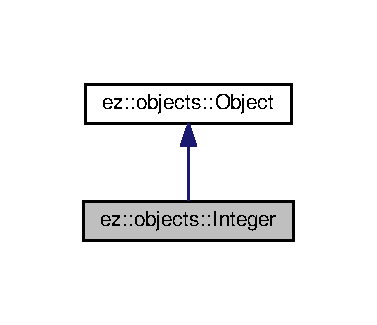
\includegraphics[width=181pt]{classez_1_1objects_1_1Integer__inherit__graph}
\end{center}
\end{figure}


Collaboration diagram for ez\+:\+:objects\+:\+:Integer\+:
\nopagebreak
\begin{figure}[H]
\begin{center}
\leavevmode
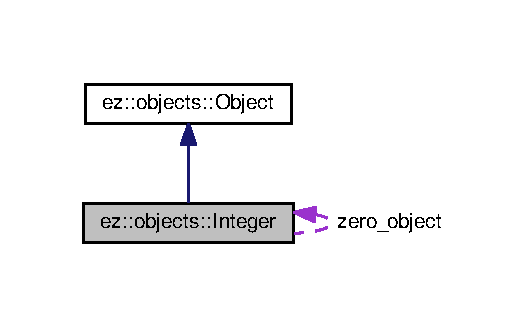
\includegraphics[width=253pt]{classez_1_1objects_1_1Integer__coll__graph}
\end{center}
\end{figure}
\subsection*{Public Types}
\begin{DoxyCompactItemize}
\item 
\mbox{\Hypertarget{classez_1_1objects_1_1Integer_a54d5c86b73369ceacc24cb50211967ec}\label{classez_1_1objects_1_1Integer_a54d5c86b73369ceacc24cb50211967ec}} 
typedef \hyperlink{classez_1_1objects_1_1Integer}{Integer} {\bfseries self}
\end{DoxyCompactItemize}
\subsection*{Public Member Functions}
\begin{DoxyCompactItemize}
\item 
\hyperlink{classez_1_1objects_1_1Integer_affb53a3df3747d3571f59533fb806a7f}{Integer} ()
\item 
\hyperlink{classez_1_1objects_1_1Integer_abbfeeb57ba1420103085e186c1aedb75}{Integer} (integer x)
\item 
\hyperlink{classez_1_1objects_1_1Integer_a0c7e18a60b0f3ecef05be8c969fcebc9}{Integer} (const \hyperlink{classez_1_1objects_1_1Integer}{Integer} \&obj)
\item 
\hyperlink{classez_1_1objects_1_1Integer}{Integer} \& \hyperlink{classez_1_1objects_1_1Integer_ae52610e2e76d891ac3c559c2b2d5ff3e}{operator=} (const \hyperlink{classez_1_1objects_1_1Integer}{Integer} \&obj)
\item 
\hyperlink{classez_1_1objects_1_1Integer_a0fd905ab5b0c4f22118e77da28a5bd66}{$\sim$\+Integer} ()
\item 
\mbox{\Hypertarget{classez_1_1objects_1_1Integer_a460e2f806a754e765bf5c6dbe1206cc8}\label{classez_1_1objects_1_1Integer_a460e2f806a754e765bf5c6dbe1206cc8}} 
integer {\bfseries value} ()
\item 
\mbox{\Hypertarget{classez_1_1objects_1_1Integer_a393519e75f5d9996acb2ea901a51552a}\label{classez_1_1objects_1_1Integer_a393519e75f5d9996acb2ea901a51552a}} 
void {\bfseries value} (integer i)
\item 
void \hyperlink{classez_1_1objects_1_1Integer_a4d358be1f412fd702bd332cc4bf113bf}{print} (std\+::ostream \&stream)
\item 
void \hyperlink{classez_1_1objects_1_1Integer_ab6035639fbee8c61086db044b731e213}{output} (std\+::ostream \&stream)
\item 
void \hyperlink{classez_1_1objects_1_1Integer_af465d88d1b132f7131be7b29aadc5a8f}{input} (std\+::istream \&stream)
\item 
\hyperlink{classez_1_1objects_1_1Object}{Object} $\ast$ \hyperlink{classez_1_1objects_1_1Integer_a83913903bdcb955ae11a08d12d9e26c6}{clone} ()
\item 
bool \hyperlink{classez_1_1objects_1_1Integer_a8b35ec8937520b2227650aa489427bcd}{is\+\_\+numeric} ()
\item 
integer \hyperlink{classez_1_1objects_1_1Integer_ab49e5990b97a97b1954dfa9222d29c82}{compare} (const \hyperlink{classez_1_1objects_1_1Object}{Object} \&y)
\item 
integer \hyperlink{classez_1_1objects_1_1Integer_a037a0eb32dd0f3d24cb54de41c199600}{factorial} ()
\item 
\mbox{\Hypertarget{classez_1_1objects_1_1Integer_a231bee5dff61d774af4f2509d113a3bd}\label{classez_1_1objects_1_1Integer_a231bee5dff61d774af4f2509d113a3bd}} 
integer {\bfseries fibonacci} ()
\item 
\mbox{\Hypertarget{classez_1_1objects_1_1Integer_a4d39b5eed04f87581ef8a336c0f10d4b}\label{classez_1_1objects_1_1Integer_a4d39b5eed04f87581ef8a336c0f10d4b}} 
integer {\bfseries sqrt} ()
\item 
\mbox{\Hypertarget{classez_1_1objects_1_1Integer_aba53aebd0c9a4963c16080b591f4fd32}\label{classez_1_1objects_1_1Integer_aba53aebd0c9a4963c16080b591f4fd32}} 
bool {\bfseries is\+\_\+prime} ()
\item 
\mbox{\Hypertarget{classez_1_1objects_1_1Integer_a86351949dee693f6b389eb8047b3f022}\label{classez_1_1objects_1_1Integer_a86351949dee693f6b389eb8047b3f022}} 
\hyperlink{classez_1_1objects_1_1Integer}{self} \& {\bfseries operator+=} (const \hyperlink{classez_1_1objects_1_1Integer}{self} \&y)
\item 
\mbox{\Hypertarget{classez_1_1objects_1_1Integer_a9bb221ab4455f8e34c85de48243ac5a8}\label{classez_1_1objects_1_1Integer_a9bb221ab4455f8e34c85de48243ac5a8}} 
\hyperlink{classez_1_1objects_1_1Integer}{self} \& {\bfseries operator-\/=} (const \hyperlink{classez_1_1objects_1_1Integer}{self} \&y)
\item 
\mbox{\Hypertarget{classez_1_1objects_1_1Integer_a1bfc55053365fb0b73cd9efa6b2c09ae}\label{classez_1_1objects_1_1Integer_a1bfc55053365fb0b73cd9efa6b2c09ae}} 
\hyperlink{classez_1_1objects_1_1Integer}{self} \& {\bfseries operator/=} (const \hyperlink{classez_1_1objects_1_1Integer}{self} \&y)
\item 
\mbox{\Hypertarget{classez_1_1objects_1_1Integer_a1ad6688f266a7aa073998b111dd4933a}\label{classez_1_1objects_1_1Integer_a1ad6688f266a7aa073998b111dd4933a}} 
\hyperlink{classez_1_1objects_1_1Integer}{self} \& {\bfseries operator$\ast$=} (const \hyperlink{classez_1_1objects_1_1Integer}{self} \&y)
\item 
\mbox{\Hypertarget{classez_1_1objects_1_1Integer_a4b479d6b9508ff53fbbab7ec1a415a9b}\label{classez_1_1objects_1_1Integer_a4b479d6b9508ff53fbbab7ec1a415a9b}} 
\hyperlink{classez_1_1objects_1_1Integer}{self} \& {\bfseries operator++} ()
\item 
\mbox{\Hypertarget{classez_1_1objects_1_1Integer_a6786340c56dad2b66fe07aa6b9996d6c}\label{classez_1_1objects_1_1Integer_a6786340c56dad2b66fe07aa6b9996d6c}} 
\hyperlink{classez_1_1objects_1_1Integer}{self} {\bfseries operator++} (int junk)
\item 
\mbox{\Hypertarget{classez_1_1objects_1_1Integer_a1da5a005cd4ae1e2741e5ddb70b75673}\label{classez_1_1objects_1_1Integer_a1da5a005cd4ae1e2741e5ddb70b75673}} 
\hyperlink{classez_1_1objects_1_1Integer}{self} \& {\bfseries operator-\/-\/} ()
\item 
\mbox{\Hypertarget{classez_1_1objects_1_1Integer_ab048d4dcc7bbdd14c632aee899a13e98}\label{classez_1_1objects_1_1Integer_ab048d4dcc7bbdd14c632aee899a13e98}} 
\hyperlink{classez_1_1objects_1_1Integer}{self} {\bfseries operator-\/-\/} (int junk)
\end{DoxyCompactItemize}
\subsection*{Static Public Member Functions}
\begin{DoxyCompactItemize}
\item 
static integer \hyperlink{classez_1_1objects_1_1Integer_a16573c56739262f5a869774c2a090d27}{factorial} (integer x)
\item 
static integer \hyperlink{classez_1_1objects_1_1Integer_ad85fb9d0675b07672d5dc9a8903e855c}{fibonacci} (integer x)
\item 
static integer \hyperlink{classez_1_1objects_1_1Integer_aebf04168540a887d84e74df2df79a404}{sqrt} (integer x)
\item 
static bool \hyperlink{classez_1_1objects_1_1Integer_a27467dd30f1b4d62119bc5630f6633d6}{is\+\_\+prime} (integer x)
\end{DoxyCompactItemize}
\subsection*{Data Fields}
\begin{DoxyCompactItemize}
\item 
integer \hyperlink{classez_1_1objects_1_1Integer_aafa80bd51f80360ca9f13e740ecd13ff}{m\+\_\+value}
\end{DoxyCompactItemize}
\subsection*{Static Public Attributes}
\begin{DoxyCompactItemize}
\item 
static integer \hyperlink{classez_1_1objects_1_1Integer_a55fb158fee3051e1dc48aa12e95b3890}{zero} = 0
\item 
static \hyperlink{classez_1_1objects_1_1Integer}{Integer} \hyperlink{classez_1_1objects_1_1Integer_a2a58362ca8067e5b72afa37968ad28ee}{zero\+\_\+object}
\end{DoxyCompactItemize}
\subsection*{Friends}
\begin{DoxyCompactItemize}
\item 
\mbox{\Hypertarget{classez_1_1objects_1_1Integer_ac219ecb06730e7707b9bb78b5da63c3b}\label{classez_1_1objects_1_1Integer_ac219ecb06730e7707b9bb78b5da63c3b}} 
\hyperlink{classez_1_1objects_1_1Integer}{self} {\bfseries operator+} (const \hyperlink{classez_1_1objects_1_1Integer}{self} x, const \hyperlink{classez_1_1objects_1_1Integer}{self} y)
\item 
\mbox{\Hypertarget{classez_1_1objects_1_1Integer_a6750cba02a1d652b1bd892bfba555e50}\label{classez_1_1objects_1_1Integer_a6750cba02a1d652b1bd892bfba555e50}} 
\hyperlink{classez_1_1objects_1_1Integer}{self} {\bfseries operator-\/} (const \hyperlink{classez_1_1objects_1_1Integer}{self} x, const \hyperlink{classez_1_1objects_1_1Integer}{self} y)
\item 
\mbox{\Hypertarget{classez_1_1objects_1_1Integer_a4f9af882c7a074ed8e1f8da41bd31dc9}\label{classez_1_1objects_1_1Integer_a4f9af882c7a074ed8e1f8da41bd31dc9}} 
\hyperlink{classez_1_1objects_1_1Integer}{self} {\bfseries operator$\ast$} (const \hyperlink{classez_1_1objects_1_1Integer}{self} x, const \hyperlink{classez_1_1objects_1_1Integer}{self} y)
\item 
\mbox{\Hypertarget{classez_1_1objects_1_1Integer_aa69c5e8b6898bb99a6f4d6e8962560c8}\label{classez_1_1objects_1_1Integer_aa69c5e8b6898bb99a6f4d6e8962560c8}} 
\hyperlink{classez_1_1objects_1_1Integer}{self} {\bfseries operator/} (const \hyperlink{classez_1_1objects_1_1Integer}{self} x, const \hyperlink{classez_1_1objects_1_1Integer}{self} y)
\end{DoxyCompactItemize}


\subsection{Detailed Description}
Class used to represent an integer 

\subsection{Constructor \& Destructor Documentation}
\mbox{\Hypertarget{classez_1_1objects_1_1Integer_affb53a3df3747d3571f59533fb806a7f}\label{classez_1_1objects_1_1Integer_affb53a3df3747d3571f59533fb806a7f}} 
\index{ez\+::objects\+::\+Integer@{ez\+::objects\+::\+Integer}!Integer@{Integer}}
\index{Integer@{Integer}!ez\+::objects\+::\+Integer@{ez\+::objects\+::\+Integer}}
\subsubsection{\texorpdfstring{Integer()}{Integer()}\hspace{0.1cm}{\footnotesize\ttfamily [1/3]}}
{\footnotesize\ttfamily ez\+::objects\+::\+Integer\+::\+Integer (\begin{DoxyParamCaption}{ }\end{DoxyParamCaption})\hspace{0.3cm}{\ttfamily [inline]}}

default constructor \mbox{\Hypertarget{classez_1_1objects_1_1Integer_abbfeeb57ba1420103085e186c1aedb75}\label{classez_1_1objects_1_1Integer_abbfeeb57ba1420103085e186c1aedb75}} 
\index{ez\+::objects\+::\+Integer@{ez\+::objects\+::\+Integer}!Integer@{Integer}}
\index{Integer@{Integer}!ez\+::objects\+::\+Integer@{ez\+::objects\+::\+Integer}}
\subsubsection{\texorpdfstring{Integer()}{Integer()}\hspace{0.1cm}{\footnotesize\ttfamily [2/3]}}
{\footnotesize\ttfamily ez\+::objects\+::\+Integer\+::\+Integer (\begin{DoxyParamCaption}\item[{integer}]{x }\end{DoxyParamCaption})\hspace{0.3cm}{\ttfamily [inline]}}

constructor given an initial value \mbox{\Hypertarget{classez_1_1objects_1_1Integer_a0c7e18a60b0f3ecef05be8c969fcebc9}\label{classez_1_1objects_1_1Integer_a0c7e18a60b0f3ecef05be8c969fcebc9}} 
\index{ez\+::objects\+::\+Integer@{ez\+::objects\+::\+Integer}!Integer@{Integer}}
\index{Integer@{Integer}!ez\+::objects\+::\+Integer@{ez\+::objects\+::\+Integer}}
\subsubsection{\texorpdfstring{Integer()}{Integer()}\hspace{0.1cm}{\footnotesize\ttfamily [3/3]}}
{\footnotesize\ttfamily ez\+::objects\+::\+Integer\+::\+Integer (\begin{DoxyParamCaption}\item[{const \hyperlink{classez_1_1objects_1_1Integer}{Integer} \&}]{obj }\end{DoxyParamCaption})\hspace{0.3cm}{\ttfamily [inline]}}

copy constructor \mbox{\Hypertarget{classez_1_1objects_1_1Integer_a0fd905ab5b0c4f22118e77da28a5bd66}\label{classez_1_1objects_1_1Integer_a0fd905ab5b0c4f22118e77da28a5bd66}} 
\index{ez\+::objects\+::\+Integer@{ez\+::objects\+::\+Integer}!````~Integer@{$\sim$\+Integer}}
\index{````~Integer@{$\sim$\+Integer}!ez\+::objects\+::\+Integer@{ez\+::objects\+::\+Integer}}
\subsubsection{\texorpdfstring{$\sim$\+Integer()}{~Integer()}}
{\footnotesize\ttfamily ez\+::objects\+::\+Integer\+::$\sim$\+Integer (\begin{DoxyParamCaption}{ }\end{DoxyParamCaption})\hspace{0.3cm}{\ttfamily [inline]}}

destructor 

\subsection{Member Function Documentation}
\mbox{\Hypertarget{classez_1_1objects_1_1Integer_a83913903bdcb955ae11a08d12d9e26c6}\label{classez_1_1objects_1_1Integer_a83913903bdcb955ae11a08d12d9e26c6}} 
\index{ez\+::objects\+::\+Integer@{ez\+::objects\+::\+Integer}!clone@{clone}}
\index{clone@{clone}!ez\+::objects\+::\+Integer@{ez\+::objects\+::\+Integer}}
\subsubsection{\texorpdfstring{clone()}{clone()}}
{\footnotesize\ttfamily \hyperlink{classez_1_1objects_1_1Object}{Object}$\ast$ ez\+::objects\+::\+Integer\+::clone (\begin{DoxyParamCaption}{ }\end{DoxyParamCaption})\hspace{0.3cm}{\ttfamily [inline]}, {\ttfamily [virtual]}}

return a copy of the object 

Reimplemented from \hyperlink{classez_1_1objects_1_1Object_acf444b2581d898eb4b8c92c2d5865c9e}{ez\+::objects\+::\+Object}.

\mbox{\Hypertarget{classez_1_1objects_1_1Integer_ab49e5990b97a97b1954dfa9222d29c82}\label{classez_1_1objects_1_1Integer_ab49e5990b97a97b1954dfa9222d29c82}} 
\index{ez\+::objects\+::\+Integer@{ez\+::objects\+::\+Integer}!compare@{compare}}
\index{compare@{compare}!ez\+::objects\+::\+Integer@{ez\+::objects\+::\+Integer}}
\subsubsection{\texorpdfstring{compare()}{compare()}}
{\footnotesize\ttfamily integer ez\+::objects\+::\+Integer\+::compare (\begin{DoxyParamCaption}\item[{const \hyperlink{classez_1_1objects_1_1Object}{Object} \&}]{y }\end{DoxyParamCaption})\hspace{0.3cm}{\ttfamily [inline]}, {\ttfamily [virtual]}}

equality between objects 

Reimplemented from \hyperlink{classez_1_1objects_1_1Object_aca311d389dffa204e425463145f4e1e6}{ez\+::objects\+::\+Object}.

\mbox{\Hypertarget{classez_1_1objects_1_1Integer_a16573c56739262f5a869774c2a090d27}\label{classez_1_1objects_1_1Integer_a16573c56739262f5a869774c2a090d27}} 
\index{ez\+::objects\+::\+Integer@{ez\+::objects\+::\+Integer}!factorial@{factorial}}
\index{factorial@{factorial}!ez\+::objects\+::\+Integer@{ez\+::objects\+::\+Integer}}
\subsubsection{\texorpdfstring{factorial()}{factorial()}\hspace{0.1cm}{\footnotesize\ttfamily [1/2]}}
{\footnotesize\ttfamily integer Integer\+::factorial (\begin{DoxyParamCaption}\item[{integer}]{x }\end{DoxyParamCaption})\hspace{0.3cm}{\ttfamily [static]}}

compute factorial of an \hyperlink{classez_1_1objects_1_1Integer}{Integer} \mbox{\Hypertarget{classez_1_1objects_1_1Integer_a037a0eb32dd0f3d24cb54de41c199600}\label{classez_1_1objects_1_1Integer_a037a0eb32dd0f3d24cb54de41c199600}} 
\index{ez\+::objects\+::\+Integer@{ez\+::objects\+::\+Integer}!factorial@{factorial}}
\index{factorial@{factorial}!ez\+::objects\+::\+Integer@{ez\+::objects\+::\+Integer}}
\subsubsection{\texorpdfstring{factorial()}{factorial()}\hspace{0.1cm}{\footnotesize\ttfamily [2/2]}}
{\footnotesize\ttfamily integer ez\+::objects\+::\+Integer\+::factorial (\begin{DoxyParamCaption}{ }\end{DoxyParamCaption})\hspace{0.3cm}{\ttfamily [inline]}}

compute factorial of this \hyperlink{classez_1_1objects_1_1Integer}{Integer} \begin{DoxyReturn}{Returns}
factorial is in allowed range of values 
\end{DoxyReturn}
\mbox{\Hypertarget{classez_1_1objects_1_1Integer_ad85fb9d0675b07672d5dc9a8903e855c}\label{classez_1_1objects_1_1Integer_ad85fb9d0675b07672d5dc9a8903e855c}} 
\index{ez\+::objects\+::\+Integer@{ez\+::objects\+::\+Integer}!fibonacci@{fibonacci}}
\index{fibonacci@{fibonacci}!ez\+::objects\+::\+Integer@{ez\+::objects\+::\+Integer}}
\subsubsection{\texorpdfstring{fibonacci()}{fibonacci()}}
{\footnotesize\ttfamily integer Integer\+::fibonacci (\begin{DoxyParamCaption}\item[{integer}]{x }\end{DoxyParamCaption})\hspace{0.3cm}{\ttfamily [static]}}

compute fibonacci of an \hyperlink{classez_1_1objects_1_1Integer}{Integer} \mbox{\Hypertarget{classez_1_1objects_1_1Integer_af465d88d1b132f7131be7b29aadc5a8f}\label{classez_1_1objects_1_1Integer_af465d88d1b132f7131be7b29aadc5a8f}} 
\index{ez\+::objects\+::\+Integer@{ez\+::objects\+::\+Integer}!input@{input}}
\index{input@{input}!ez\+::objects\+::\+Integer@{ez\+::objects\+::\+Integer}}
\subsubsection{\texorpdfstring{input()}{input()}}
{\footnotesize\ttfamily void Integer\+::input (\begin{DoxyParamCaption}\item[{std\+::istream \&}]{stream }\end{DoxyParamCaption})\hspace{0.3cm}{\ttfamily [virtual]}}

this function is used to get the data field members of an object from a stream and acts as unserialize 

Reimplemented from \hyperlink{classez_1_1objects_1_1Object_a878bdc53b7f16fda6fa15dab214c4b6a}{ez\+::objects\+::\+Object}.

\mbox{\Hypertarget{classez_1_1objects_1_1Integer_a8b35ec8937520b2227650aa489427bcd}\label{classez_1_1objects_1_1Integer_a8b35ec8937520b2227650aa489427bcd}} 
\index{ez\+::objects\+::\+Integer@{ez\+::objects\+::\+Integer}!is\+\_\+numeric@{is\+\_\+numeric}}
\index{is\+\_\+numeric@{is\+\_\+numeric}!ez\+::objects\+::\+Integer@{ez\+::objects\+::\+Integer}}
\subsubsection{\texorpdfstring{is\+\_\+numeric()}{is\_numeric()}}
{\footnotesize\ttfamily bool ez\+::objects\+::\+Integer\+::is\+\_\+numeric (\begin{DoxyParamCaption}{ }\end{DoxyParamCaption})\hspace{0.3cm}{\ttfamily [inline]}, {\ttfamily [virtual]}}

indicates if this object can be used for computation 

Reimplemented from \hyperlink{classez_1_1objects_1_1Object_a19ba1672d4063232c4619e016ca178f8}{ez\+::objects\+::\+Object}.

\mbox{\Hypertarget{classez_1_1objects_1_1Integer_a27467dd30f1b4d62119bc5630f6633d6}\label{classez_1_1objects_1_1Integer_a27467dd30f1b4d62119bc5630f6633d6}} 
\index{ez\+::objects\+::\+Integer@{ez\+::objects\+::\+Integer}!is\+\_\+prime@{is\+\_\+prime}}
\index{is\+\_\+prime@{is\+\_\+prime}!ez\+::objects\+::\+Integer@{ez\+::objects\+::\+Integer}}
\subsubsection{\texorpdfstring{is\+\_\+prime()}{is\_prime()}}
{\footnotesize\ttfamily bool Integer\+::is\+\_\+prime (\begin{DoxyParamCaption}\item[{integer}]{x }\end{DoxyParamCaption})\hspace{0.3cm}{\ttfamily [static]}}

check if given integer x is prime \begin{DoxyReturn}{Returns}
true if x is a prime number 
\end{DoxyReturn}
\mbox{\Hypertarget{classez_1_1objects_1_1Integer_ae52610e2e76d891ac3c559c2b2d5ff3e}\label{classez_1_1objects_1_1Integer_ae52610e2e76d891ac3c559c2b2d5ff3e}} 
\index{ez\+::objects\+::\+Integer@{ez\+::objects\+::\+Integer}!operator=@{operator=}}
\index{operator=@{operator=}!ez\+::objects\+::\+Integer@{ez\+::objects\+::\+Integer}}
\subsubsection{\texorpdfstring{operator=()}{operator=()}}
{\footnotesize\ttfamily \hyperlink{classez_1_1objects_1_1Integer}{Integer}\& ez\+::objects\+::\+Integer\+::operator= (\begin{DoxyParamCaption}\item[{const \hyperlink{classez_1_1objects_1_1Integer}{Integer} \&}]{obj }\end{DoxyParamCaption})\hspace{0.3cm}{\ttfamily [inline]}}

assignment operator \mbox{\Hypertarget{classez_1_1objects_1_1Integer_ab6035639fbee8c61086db044b731e213}\label{classez_1_1objects_1_1Integer_ab6035639fbee8c61086db044b731e213}} 
\index{ez\+::objects\+::\+Integer@{ez\+::objects\+::\+Integer}!output@{output}}
\index{output@{output}!ez\+::objects\+::\+Integer@{ez\+::objects\+::\+Integer}}
\subsubsection{\texorpdfstring{output()}{output()}}
{\footnotesize\ttfamily void Integer\+::output (\begin{DoxyParamCaption}\item[{std\+::ostream \&}]{stream }\end{DoxyParamCaption})\hspace{0.3cm}{\ttfamily [virtual]}}

this function is used to print the contents of the object in a serializable manner 

Reimplemented from \hyperlink{classez_1_1objects_1_1Object_a0fdfe18e6c35d6b0d7e7a01265aded15}{ez\+::objects\+::\+Object}.

\mbox{\Hypertarget{classez_1_1objects_1_1Integer_a4d358be1f412fd702bd332cc4bf113bf}\label{classez_1_1objects_1_1Integer_a4d358be1f412fd702bd332cc4bf113bf}} 
\index{ez\+::objects\+::\+Integer@{ez\+::objects\+::\+Integer}!print@{print}}
\index{print@{print}!ez\+::objects\+::\+Integer@{ez\+::objects\+::\+Integer}}
\subsubsection{\texorpdfstring{print()}{print()}}
{\footnotesize\ttfamily void Integer\+::print (\begin{DoxyParamCaption}\item[{std\+::ostream \&}]{stream }\end{DoxyParamCaption})\hspace{0.3cm}{\ttfamily [virtual]}}

this function is used to print the contents of the object in a human readable format 
\begin{DoxyParams}{Parameters}
{\em stream} & output stream for example std\+::cout \\
\hline
\end{DoxyParams}


Reimplemented from \hyperlink{classez_1_1objects_1_1Object_a9e20f39a78163f67f000576149d858b3}{ez\+::objects\+::\+Object}.

\mbox{\Hypertarget{classez_1_1objects_1_1Integer_aebf04168540a887d84e74df2df79a404}\label{classez_1_1objects_1_1Integer_aebf04168540a887d84e74df2df79a404}} 
\index{ez\+::objects\+::\+Integer@{ez\+::objects\+::\+Integer}!sqrt@{sqrt}}
\index{sqrt@{sqrt}!ez\+::objects\+::\+Integer@{ez\+::objects\+::\+Integer}}
\subsubsection{\texorpdfstring{sqrt()}{sqrt()}}
{\footnotesize\ttfamily integer Integer\+::sqrt (\begin{DoxyParamCaption}\item[{integer}]{x }\end{DoxyParamCaption})\hspace{0.3cm}{\ttfamily [static]}}

compute square root of an \hyperlink{classez_1_1objects_1_1Integer}{Integer}. The value is rounded to the nearest integer 

\subsection{Field Documentation}
\mbox{\Hypertarget{classez_1_1objects_1_1Integer_aafa80bd51f80360ca9f13e740ecd13ff}\label{classez_1_1objects_1_1Integer_aafa80bd51f80360ca9f13e740ecd13ff}} 
\index{ez\+::objects\+::\+Integer@{ez\+::objects\+::\+Integer}!m\+\_\+value@{m\+\_\+value}}
\index{m\+\_\+value@{m\+\_\+value}!ez\+::objects\+::\+Integer@{ez\+::objects\+::\+Integer}}
\subsubsection{\texorpdfstring{m\+\_\+value}{m\_value}}
{\footnotesize\ttfamily integer ez\+::objects\+::\+Integer\+::m\+\_\+value}

value stored \mbox{\Hypertarget{classez_1_1objects_1_1Integer_a55fb158fee3051e1dc48aa12e95b3890}\label{classez_1_1objects_1_1Integer_a55fb158fee3051e1dc48aa12e95b3890}} 
\index{ez\+::objects\+::\+Integer@{ez\+::objects\+::\+Integer}!zero@{zero}}
\index{zero@{zero}!ez\+::objects\+::\+Integer@{ez\+::objects\+::\+Integer}}
\subsubsection{\texorpdfstring{zero}{zero}}
{\footnotesize\ttfamily integer Integer\+::zero = 0\hspace{0.3cm}{\ttfamily [static]}}

Zero constant \mbox{\Hypertarget{classez_1_1objects_1_1Integer_a2a58362ca8067e5b72afa37968ad28ee}\label{classez_1_1objects_1_1Integer_a2a58362ca8067e5b72afa37968ad28ee}} 
\index{ez\+::objects\+::\+Integer@{ez\+::objects\+::\+Integer}!zero\+\_\+object@{zero\+\_\+object}}
\index{zero\+\_\+object@{zero\+\_\+object}!ez\+::objects\+::\+Integer@{ez\+::objects\+::\+Integer}}
\subsubsection{\texorpdfstring{zero\+\_\+object}{zero\_object}}
{\footnotesize\ttfamily \hyperlink{classez_1_1objects_1_1Integer}{Integer} Integer\+::zero\+\_\+object\hspace{0.3cm}{\ttfamily [static]}}

Zero object constant 

The documentation for this class was generated from the following files\+:\begin{DoxyCompactItemize}
\item 
src/version\+\_\+2018.\+06/objects/integer.\+h\item 
src/version\+\_\+2018.\+06/objects/integer.\+cpp\end{DoxyCompactItemize}

\hypertarget{classez_1_1arguments_1_1IntegerArgument}{}\section{ez\+:\+:arguments\+:\+:Integer\+Argument Class Reference}
\label{classez_1_1arguments_1_1IntegerArgument}\index{ez\+::arguments\+::\+Integer\+Argument@{ez\+::arguments\+::\+Integer\+Argument}}


{\ttfamily \#include $<$integer\+\_\+argument.\+h$>$}



Inheritance diagram for ez\+:\+:arguments\+:\+:Integer\+Argument\+:
\nopagebreak
\begin{figure}[H]
\begin{center}
\leavevmode
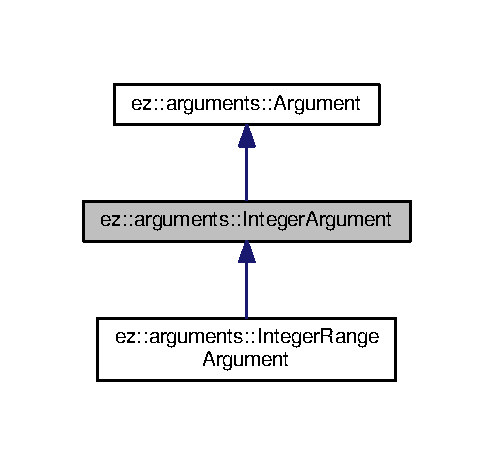
\includegraphics[width=237pt]{classez_1_1arguments_1_1IntegerArgument__inherit__graph}
\end{center}
\end{figure}


Collaboration diagram for ez\+:\+:arguments\+:\+:Integer\+Argument\+:
\nopagebreak
\begin{figure}[H]
\begin{center}
\leavevmode
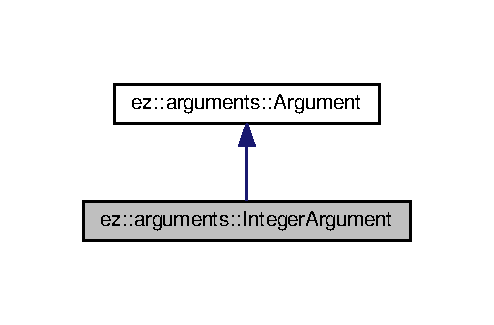
\includegraphics[width=237pt]{classez_1_1arguments_1_1IntegerArgument__coll__graph}
\end{center}
\end{figure}
\subsection*{Public Member Functions}
\begin{DoxyCompactItemize}
\item 
\mbox{\Hypertarget{classez_1_1arguments_1_1IntegerArgument_a69f681b2f4ac32f560c32c77818c348b}\label{classez_1_1arguments_1_1IntegerArgument_a69f681b2f4ac32f560c32c77818c348b}} 
{\bfseries Integer\+Argument} (string long\+\_\+label, char short\+\_\+label, integer $\ast$value, string description, trigger\+\_\+t trigger=nullptr)
\item 
\mbox{\Hypertarget{classez_1_1arguments_1_1IntegerArgument_a35f36b08ea78d1e8461f442064c8ddb2}\label{classez_1_1arguments_1_1IntegerArgument_a35f36b08ea78d1e8461f442064c8ddb2}} 
void {\bfseries parse} (string \&s)
\end{DoxyCompactItemize}
\subsection*{Protected Attributes}
\begin{DoxyCompactItemize}
\item 
\mbox{\Hypertarget{classez_1_1arguments_1_1IntegerArgument_ae26dba714e3795690f9bc33fbe0f6b4d}\label{classez_1_1arguments_1_1IntegerArgument_ae26dba714e3795690f9bc33fbe0f6b4d}} 
integer $\ast$ {\bfseries m\+\_\+value}
\end{DoxyCompactItemize}


\subsection{Detailed Description}
class used to treat integer argument 

The documentation for this class was generated from the following files\+:\begin{DoxyCompactItemize}
\item 
src/version\+\_\+2018.\+06/arguments/integer\+\_\+argument.\+h\item 
src/version\+\_\+2018.\+06/arguments/integer\+\_\+argument.\+cpp\end{DoxyCompactItemize}

\hypertarget{classez_1_1arguments_1_1IntegerRangeArgument}{}\section{ez\+:\+:arguments\+:\+:Integer\+Range\+Argument Class Reference}
\label{classez_1_1arguments_1_1IntegerRangeArgument}\index{ez\+::arguments\+::\+Integer\+Range\+Argument@{ez\+::arguments\+::\+Integer\+Range\+Argument}}


{\ttfamily \#include $<$integer\+\_\+range\+\_\+argument.\+h$>$}



Inheritance diagram for ez\+:\+:arguments\+:\+:Integer\+Range\+Argument\+:
\nopagebreak
\begin{figure}[H]
\begin{center}
\leavevmode
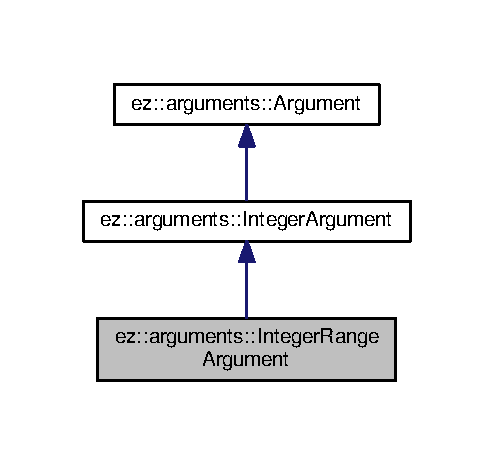
\includegraphics[width=237pt]{classez_1_1arguments_1_1IntegerRangeArgument__inherit__graph}
\end{center}
\end{figure}


Collaboration diagram for ez\+:\+:arguments\+:\+:Integer\+Range\+Argument\+:
\nopagebreak
\begin{figure}[H]
\begin{center}
\leavevmode
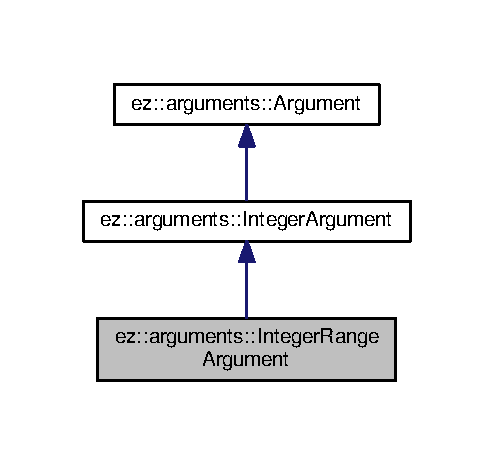
\includegraphics[width=237pt]{classez_1_1arguments_1_1IntegerRangeArgument__coll__graph}
\end{center}
\end{figure}
\subsection*{Public Member Functions}
\begin{DoxyCompactItemize}
\item 
\mbox{\Hypertarget{classez_1_1arguments_1_1IntegerRangeArgument_aca1a6753aeff2e3acd4e8c8899de790b}\label{classez_1_1arguments_1_1IntegerRangeArgument_aca1a6753aeff2e3acd4e8c8899de790b}} 
{\bfseries Integer\+Range\+Argument} (string long\+\_\+label, char short\+\_\+label, integer $\ast$value, integer mini, integer maxi, string description, trigger\+\_\+t trigger=nullptr)
\item 
\mbox{\Hypertarget{classez_1_1arguments_1_1IntegerRangeArgument_ac167a406461c11e1076c8e703a516bac}\label{classez_1_1arguments_1_1IntegerRangeArgument_ac167a406461c11e1076c8e703a516bac}} 
void {\bfseries parse} (string \&s)
\item 
\mbox{\Hypertarget{classez_1_1arguments_1_1IntegerRangeArgument_a74cbc2ba7fb0c7fef92b1a02d7a0c8dc}\label{classez_1_1arguments_1_1IntegerRangeArgument_a74cbc2ba7fb0c7fef92b1a02d7a0c8dc}} 
integer {\bfseries min} ()
\item 
\mbox{\Hypertarget{classez_1_1arguments_1_1IntegerRangeArgument_ad47993387de8e32bf9555241d2781be2}\label{classez_1_1arguments_1_1IntegerRangeArgument_ad47993387de8e32bf9555241d2781be2}} 
integer {\bfseries max} ()
\end{DoxyCompactItemize}
\subsection*{Protected Attributes}
\begin{DoxyCompactItemize}
\item 
\mbox{\Hypertarget{classez_1_1arguments_1_1IntegerRangeArgument_a40b579d4c4d7e112b5a881e35b01a858}\label{classez_1_1arguments_1_1IntegerRangeArgument_a40b579d4c4d7e112b5a881e35b01a858}} 
integer {\bfseries m\+\_\+min\+\_\+value}
\item 
\mbox{\Hypertarget{classez_1_1arguments_1_1IntegerRangeArgument_a2812cb927573632aafa2fd65379ef741}\label{classez_1_1arguments_1_1IntegerRangeArgument_a2812cb927573632aafa2fd65379ef741}} 
integer {\bfseries m\+\_\+max\+\_\+value}
\end{DoxyCompactItemize}


\subsection{Detailed Description}
class used to treat integer range argument 

The documentation for this class was generated from the following files\+:\begin{DoxyCompactItemize}
\item 
src/version\+\_\+2018.\+06/arguments/integer\+\_\+range\+\_\+argument.\+h\item 
src/version\+\_\+2018.\+06/arguments/integer\+\_\+range\+\_\+argument.\+cpp\end{DoxyCompactItemize}

\hypertarget{classez_1_1maths_1_1Interval}{}\section{ez\+:\+:maths\+:\+:Interval$<$ T $>$ Class Template Reference}
\label{classez_1_1maths_1_1Interval}\index{ez\+::maths\+::\+Interval$<$ T $>$@{ez\+::maths\+::\+Interval$<$ T $>$}}


{\ttfamily \#include $<$interval.\+h$>$}

\subsection*{Public Member Functions}
\begin{DoxyCompactItemize}
\item 
\mbox{\Hypertarget{classez_1_1maths_1_1Interval_a1218a10c0295b667a98e046f9bed9d96}\label{classez_1_1maths_1_1Interval_a1218a10c0295b667a98e046f9bed9d96}} 
{\bfseries Interval} (T mini, T maxi)
\item 
\mbox{\Hypertarget{classez_1_1maths_1_1Interval_acbf517711d35dd1141aac089c1a2ff5e}\label{classez_1_1maths_1_1Interval_acbf517711d35dd1141aac089c1a2ff5e}} 
{\bfseries Interval} (const \hyperlink{classez_1_1maths_1_1Interval}{Interval} \&obj)
\item 
\mbox{\Hypertarget{classez_1_1maths_1_1Interval_a527a19ae2fa6939dece2ffd80b09ed46}\label{classez_1_1maths_1_1Interval_a527a19ae2fa6939dece2ffd80b09ed46}} 
bool {\bfseries contains} (T value)
\item 
\mbox{\Hypertarget{classez_1_1maths_1_1Interval_a6111df68f59687b9c871698fea164fba}\label{classez_1_1maths_1_1Interval_a6111df68f59687b9c871698fea164fba}} 
std\+::ostream \& {\bfseries print} (std\+::ostream \&out)
\item 
\mbox{\Hypertarget{classez_1_1maths_1_1Interval_a2a4c3a1d0734ec0224240994e38977b9}\label{classez_1_1maths_1_1Interval_a2a4c3a1d0734ec0224240994e38977b9}} 
T {\bfseries min} ()
\item 
\mbox{\Hypertarget{classez_1_1maths_1_1Interval_a71b16542e6fc2a4178e8aa17711f3f9b}\label{classez_1_1maths_1_1Interval_a71b16542e6fc2a4178e8aa17711f3f9b}} 
T {\bfseries max} ()
\end{DoxyCompactItemize}
\subsection*{Static Public Member Functions}
\begin{DoxyCompactItemize}
\item 
\mbox{\Hypertarget{classez_1_1maths_1_1Interval_add29d54b27ee7fdf2be4f944de5b2b56}\label{classez_1_1maths_1_1Interval_add29d54b27ee7fdf2be4f944de5b2b56}} 
static void {\bfseries generate} (std\+::vector$<$ \hyperlink{classez_1_1maths_1_1Interval}{Interval}$<$ T $>$ $>$ \&v, T lo, T hi, T incr, T delta=1)
\end{DoxyCompactItemize}
\subsection*{Protected Attributes}
\begin{DoxyCompactItemize}
\item 
\mbox{\Hypertarget{classez_1_1maths_1_1Interval_a019037c511314756bcba2b7cca453756}\label{classez_1_1maths_1_1Interval_a019037c511314756bcba2b7cca453756}} 
T {\bfseries m\+\_\+mini}
\item 
\mbox{\Hypertarget{classez_1_1maths_1_1Interval_ac22698e7c3be4ac4f2b4278f393470ef}\label{classez_1_1maths_1_1Interval_ac22698e7c3be4ac4f2b4278f393470ef}} 
T {\bfseries m\+\_\+maxi}
\end{DoxyCompactItemize}
\subsection*{Friends}
\begin{DoxyCompactItemize}
\item 
\mbox{\Hypertarget{classez_1_1maths_1_1Interval_a09cd95031ad758942e59a5de50ab51a2}\label{classez_1_1maths_1_1Interval_a09cd95031ad758942e59a5de50ab51a2}} 
bool {\bfseries operator$<$} (const \hyperlink{classez_1_1maths_1_1Interval}{Interval}$<$ T $>$ \&a, const \hyperlink{classez_1_1maths_1_1Interval}{Interval}$<$ T $>$ \&b)
\item 
\mbox{\Hypertarget{classez_1_1maths_1_1Interval_a22024bc002a0cc02281cbe6e648ed60c}\label{classez_1_1maths_1_1Interval_a22024bc002a0cc02281cbe6e648ed60c}} 
std\+::ostream \& {\bfseries operator$<$$<$} (std\+::ostream \&out, \hyperlink{classez_1_1maths_1_1Interval}{Interval}$<$ T $>$ \&obj)
\end{DoxyCompactItemize}


\subsection{Detailed Description}
\subsubsection*{template$<$class T$>$\newline
class ez\+::maths\+::\+Interval$<$ T $>$}

this class represents an \hyperlink{classez_1_1maths_1_1Interval}{Interval} from values that range into \mbox{[}x..y\mbox{]} where x $<$ y 

The documentation for this class was generated from the following file\+:\begin{DoxyCompactItemize}
\item 
src/version\+\_\+2018.\+06/maths/interval.\+h\end{DoxyCompactItemize}

\hypertarget{classez_1_1essential_1_1Range_1_1iterator}{}\section{ez\+:\+:essential\+:\+:Range\+:\+:iterator Class Reference}
\label{classez_1_1essential_1_1Range_1_1iterator}\index{ez\+::essential\+::\+Range\+::iterator@{ez\+::essential\+::\+Range\+::iterator}}


{\ttfamily \#include $<$range.\+h$>$}

\subsection*{Public Types}
\begin{DoxyCompactItemize}
\item 
\mbox{\Hypertarget{classez_1_1essential_1_1Range_1_1iterator_a713bdf44d4b985f87e10dffe035541fd}\label{classez_1_1essential_1_1Range_1_1iterator_a713bdf44d4b985f87e10dffe035541fd}} 
typedef \hyperlink{classez_1_1essential_1_1Range_1_1iterator}{iterator} {\bfseries self\+\_\+type}
\item 
\mbox{\Hypertarget{classez_1_1essential_1_1Range_1_1iterator_abb176db665ef7ba9a38d95d2bc044022}\label{classez_1_1essential_1_1Range_1_1iterator_abb176db665ef7ba9a38d95d2bc044022}} 
typedef integer {\bfseries value\+\_\+type}
\item 
\mbox{\Hypertarget{classez_1_1essential_1_1Range_1_1iterator_aa10a860a661f89117b0801607b91450e}\label{classez_1_1essential_1_1Range_1_1iterator_aa10a860a661f89117b0801607b91450e}} 
typedef integer \& {\bfseries reference}
\item 
\mbox{\Hypertarget{classez_1_1essential_1_1Range_1_1iterator_aa45fb2492e39ce4f9e2c1b13ff04704e}\label{classez_1_1essential_1_1Range_1_1iterator_aa45fb2492e39ce4f9e2c1b13ff04704e}} 
typedef integer {\bfseries pointer}
\item 
\mbox{\Hypertarget{classez_1_1essential_1_1Range_1_1iterator_abc9e68ae81132580f9091febf2ec5395}\label{classez_1_1essential_1_1Range_1_1iterator_abc9e68ae81132580f9091febf2ec5395}} 
typedef std\+::forward\+\_\+iterator\+\_\+tag {\bfseries iterator\+\_\+category}
\item 
\mbox{\Hypertarget{classez_1_1essential_1_1Range_1_1iterator_a7b590b7ff09b70ca5fac6da60c72ab28}\label{classez_1_1essential_1_1Range_1_1iterator_a7b590b7ff09b70ca5fac6da60c72ab28}} 
typedef int {\bfseries difference\+\_\+type}
\end{DoxyCompactItemize}
\subsection*{Public Member Functions}
\begin{DoxyCompactItemize}
\item 
\mbox{\Hypertarget{classez_1_1essential_1_1Range_1_1iterator_aa1a44c4ae0b2acb491168cbdbb11d018}\label{classez_1_1essential_1_1Range_1_1iterator_aa1a44c4ae0b2acb491168cbdbb11d018}} 
{\bfseries iterator} (pointer v, pointer i)
\item 
\mbox{\Hypertarget{classez_1_1essential_1_1Range_1_1iterator_af36d5567840a856e7868bf70e55b98bf}\label{classez_1_1essential_1_1Range_1_1iterator_af36d5567840a856e7868bf70e55b98bf}} 
{\bfseries iterator} (const \hyperlink{classez_1_1essential_1_1Range_1_1iterator}{iterator} \&it)
\item 
\mbox{\Hypertarget{classez_1_1essential_1_1Range_1_1iterator_a4f60e924409b3b68acaf77d820666a97}\label{classez_1_1essential_1_1Range_1_1iterator_a4f60e924409b3b68acaf77d820666a97}} 
\hyperlink{classez_1_1essential_1_1Range_1_1iterator}{iterator} \& {\bfseries operator++} ()
\item 
\mbox{\Hypertarget{classez_1_1essential_1_1Range_1_1iterator_a194e55bccf3e691f3441bf86b82ca850}\label{classez_1_1essential_1_1Range_1_1iterator_a194e55bccf3e691f3441bf86b82ca850}} 
\hyperlink{classez_1_1essential_1_1Range_1_1iterator}{iterator} {\bfseries operator++} (int junk)
\item 
\mbox{\Hypertarget{classez_1_1essential_1_1Range_1_1iterator_a5fd875db66712ec87b83aa33788c8ffa}\label{classez_1_1essential_1_1Range_1_1iterator_a5fd875db66712ec87b83aa33788c8ffa}} 
reference {\bfseries operator$\ast$} ()
\item 
\mbox{\Hypertarget{classez_1_1essential_1_1Range_1_1iterator_ace7d39f6e2251143d20333246371fd80}\label{classez_1_1essential_1_1Range_1_1iterator_ace7d39f6e2251143d20333246371fd80}} 
pointer {\bfseries operator-\/$>$} ()
\item 
\mbox{\Hypertarget{classez_1_1essential_1_1Range_1_1iterator_ae0149f2f478465a6945e4690b72fbd90}\label{classez_1_1essential_1_1Range_1_1iterator_ae0149f2f478465a6945e4690b72fbd90}} 
bool {\bfseries operator==} (const \hyperlink{classez_1_1essential_1_1Range_1_1iterator}{iterator} \&y)
\item 
\mbox{\Hypertarget{classez_1_1essential_1_1Range_1_1iterator_a761354ac7770def39f8ace39dd30bf59}\label{classez_1_1essential_1_1Range_1_1iterator_a761354ac7770def39f8ace39dd30bf59}} 
bool {\bfseries operator!=} (const \hyperlink{classez_1_1essential_1_1Range_1_1iterator}{iterator} \&y)
\end{DoxyCompactItemize}
\subsection*{Protected Attributes}
\begin{DoxyCompactItemize}
\item 
\mbox{\Hypertarget{classez_1_1essential_1_1Range_1_1iterator_ab5508b933297f8afa3d23327d22927e9}\label{classez_1_1essential_1_1Range_1_1iterator_ab5508b933297f8afa3d23327d22927e9}} 
integer {\bfseries m\+\_\+current\+\_\+value}
\item 
\mbox{\Hypertarget{classez_1_1essential_1_1Range_1_1iterator_a2ef5060eceb33714aa3fd978af5f9a59}\label{classez_1_1essential_1_1Range_1_1iterator_a2ef5060eceb33714aa3fd978af5f9a59}} 
integer {\bfseries m\+\_\+increment}
\end{DoxyCompactItemize}


\subsection{Detailed Description}
Definition of an iterator for the range which is useful for {\bfseries for} loops 

The documentation for this class was generated from the following file\+:\begin{DoxyCompactItemize}
\item 
src/version\+\_\+2018.\+06/essential/range.\+h\end{DoxyCompactItemize}

\hypertarget{classez_1_1logging_1_1Logger}{}\section{ez\+:\+:logging\+:\+:Logger Class Reference}
\label{classez_1_1logging_1_1Logger}\index{ez\+::logging\+::\+Logger@{ez\+::logging\+::\+Logger}}


{\ttfamily \#include $<$logger.\+h$>$}



Inheritance diagram for ez\+:\+:logging\+:\+:Logger\+:
\nopagebreak
\begin{figure}[H]
\begin{center}
\leavevmode
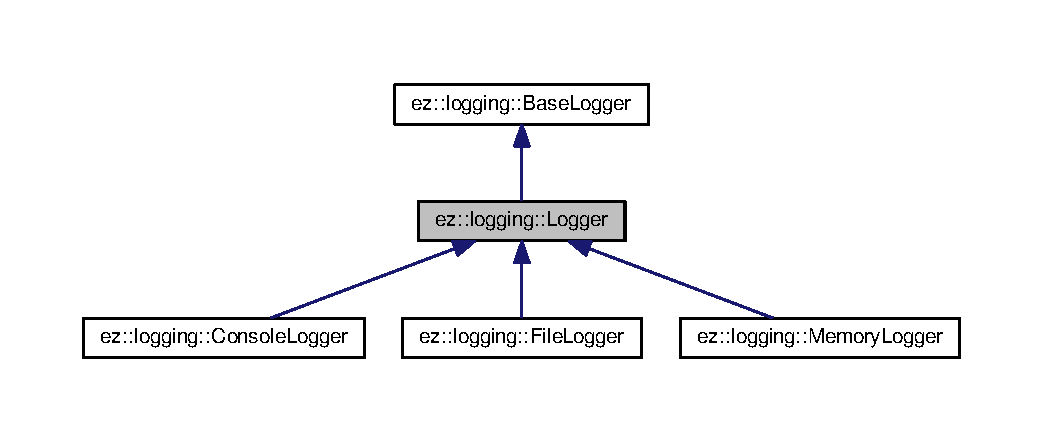
\includegraphics[width=350pt]{classez_1_1logging_1_1Logger__inherit__graph}
\end{center}
\end{figure}


Collaboration diagram for ez\+:\+:logging\+:\+:Logger\+:
\nopagebreak
\begin{figure}[H]
\begin{center}
\leavevmode
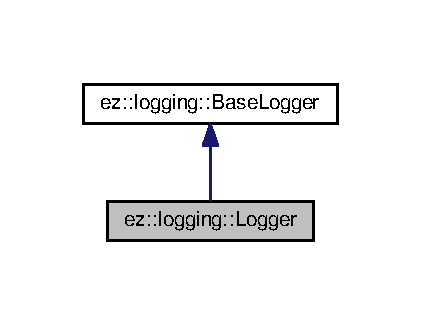
\includegraphics[width=202pt]{classez_1_1logging_1_1Logger__coll__graph}
\end{center}
\end{figure}
\subsection*{Public Member Functions}
\begin{DoxyCompactItemize}
\item 
\hyperlink{classez_1_1logging_1_1Logger_ac9465bcd94c08532b30b1801d71fbd19}{Logger} (text name, std\+::ostream $\ast$out)
\item 
virtual \hyperlink{classez_1_1logging_1_1Logger_acb668a9e186a25fbaad2e4af6d1ed00a}{$\sim$\+Logger} ()
\item 
void \hyperlink{classez_1_1logging_1_1Logger_a64bfdfc5a20a7ee660144c50dfd0514e}{set\+\_\+record\+\_\+level} (integer lvl)
\item 
void \hyperlink{classez_1_1logging_1_1Logger_a9f9bf63329c39c8f9fb116faba1a9b1e}{inc\+\_\+record\+\_\+level} ()
\item 
void \hyperlink{classez_1_1logging_1_1Logger_a337c7162a46c5e7374e80b7166cc869f}{dec\+\_\+record\+\_\+level} ()
\item 
void \hyperlink{classez_1_1logging_1_1Logger_ae9fd25392d4dc7611acafd335bfe5f94}{set\+\_\+verbose\+\_\+level} (integer lvl)
\item 
void \hyperlink{classez_1_1logging_1_1Logger_a2845727c27243d47fefbd9d65df5bd6b}{set\+\_\+header} (const char $\ast$s)
\item 
void \hyperlink{classez_1_1logging_1_1Logger_ab8e5b19223eca4b3af5ff7df2db607b7}{print\+\_\+ln} ()
\item 
void \hyperlink{classez_1_1logging_1_1Logger_a74db3d434d837a1fcdeb5a6c2326eeb3}{print} (char v)
\item 
void \hyperlink{classez_1_1logging_1_1Logger_a85f93d25c8f5eebe65b81cb72ebaea3e}{print} (integer v)
\item 
void \hyperlink{classez_1_1logging_1_1Logger_aeb154caf1a7b122fea39eb9bf6f5079a}{print} (natural v)
\item 
void \hyperlink{classez_1_1logging_1_1Logger_a20758ba23aea43e022c3198b85b8c0ed}{print} (long\+\_\+integer v)
\item 
void \hyperlink{classez_1_1logging_1_1Logger_a8c1b7b0e80f11d4b74362294fe968072}{print} (long\+\_\+natural v)
\item 
void \hyperlink{classez_1_1logging_1_1Logger_ae8367292df1035d9bc7bd09fd5ca35a7}{print} (const char $\ast$s)
\item 
void \hyperlink{classez_1_1logging_1_1Logger_a9be560bcbe68f5262eb7bd019bb8775b}{print} (string s)
\item 
void \hyperlink{classez_1_1logging_1_1Logger_a422fea2abd8a7c364e1c4846693422f1}{print} (real f)
\item 
void \hyperlink{classez_1_1logging_1_1Logger_a026763cd0c90ec5e4b5d06f08b63a140}{print} (long\+\_\+real d)
\item 
void \hyperlink{classez_1_1logging_1_1Logger_a5c8c3349b7d4aa76dfe90b1e3dc0ce00}{print} (void $\ast$p)
\item 
void \hyperlink{classez_1_1logging_1_1Logger_a3fcf2f4da96bd7a0fd33b055a23fdef3}{print} (const \hyperlink{structez_1_1logging_1_1__Setrecordlevel}{\+\_\+\+Setrecordlevel} \&lvl)
\item 
void \hyperlink{classez_1_1logging_1_1Logger_a20117d944ec1fa0aa3302981c620d8b6}{print} (const \hyperlink{structez_1_1logging_1_1__Setverboselevel}{\+\_\+\+Setverboselevel} \&lvl)
\item 
void \hyperlink{classez_1_1logging_1_1Logger_a5660d40a1364e37393b3241435ed5a64}{print} (const \hyperlink{classez_1_1essential_1_1CPUTimer}{ez\+::essential\+::\+C\+P\+U\+Timer} \&obj)
\item 
void \hyperlink{classez_1_1logging_1_1Logger_ad95b97a1ff61d4a31a0fba5e32f805a8}{print} (const \hyperlink{classez_1_1essential_1_1Range}{ez\+::essential\+::\+Range} \&obj)
\item 
\hyperlink{classez_1_1logging_1_1Logger}{Logger} \& \hyperlink{classez_1_1logging_1_1Logger_a439b87c1fdbfe851afcb3cfb29534437}{operator$<$$<$} (\hyperlink{classez_1_1logging_1_1Logger}{Logger} \&($\ast$m)(\hyperlink{classez_1_1logging_1_1Logger}{Logger} \&))
\item 
{\footnotesize template$<$class T $>$ }\\void \hyperlink{classez_1_1logging_1_1Logger_ab81b4be85f103d81e7b25a9cdf0a68e3}{print\+\_\+object} (T $\ast$obj)
\item 
ostream $\ast$ \hyperlink{classez_1_1logging_1_1Logger_a5d7092dd639907ccd702eb0df062821b}{output\+\_\+stream} ()
\item 
{\footnotesize template$<$class T $>$ }\\\hyperlink{classez_1_1logging_1_1Logger}{Logger} \& \hyperlink{classez_1_1logging_1_1Logger_a75006590ec6d4d6c8bca7d8824d887c2}{operator$<$$<$} (const T \&a)
\end{DoxyCompactItemize}
\subsection*{Static Public Member Functions}
\begin{DoxyCompactItemize}
\item 
static \hyperlink{classez_1_1logging_1_1Logger}{Logger} \& \hyperlink{classez_1_1logging_1_1Logger_a69ba6cf7130aa70caeca9f5c8636e05a}{endl} (\hyperlink{classez_1_1logging_1_1Logger}{Logger} \&l)
\end{DoxyCompactItemize}
\subsection*{Static Public Attributes}
\begin{DoxyCompactItemize}
\item 
static const integer \hyperlink{classez_1_1logging_1_1Logger_aa9ff03b52cf6bdc21b9e67086510d186}{C\+L\+O\+S\+ED} = 0
\item 
\mbox{\Hypertarget{classez_1_1logging_1_1Logger_a5255b90ac8236f172ca5e68ca051cd92}\label{classez_1_1logging_1_1Logger_a5255b90ac8236f172ca5e68ca051cd92}} 
static const integer {\bfseries L\+E\+V\+E\+L\+\_\+1} = 1
\item 
\mbox{\Hypertarget{classez_1_1logging_1_1Logger_a39efb785fbecc012ec4b43acc7f6e87b}\label{classez_1_1logging_1_1Logger_a39efb785fbecc012ec4b43acc7f6e87b}} 
static const integer {\bfseries L\+E\+V\+E\+L\+\_\+2} = 2
\item 
\mbox{\Hypertarget{classez_1_1logging_1_1Logger_ac010fadbb0dc962b7d51539a71ed8bfc}\label{classez_1_1logging_1_1Logger_ac010fadbb0dc962b7d51539a71ed8bfc}} 
static const integer {\bfseries L\+E\+V\+E\+L\+\_\+3} = 3
\item 
\mbox{\Hypertarget{classez_1_1logging_1_1Logger_aabfcb9853e1df58006702d7e5f0b581a}\label{classez_1_1logging_1_1Logger_aabfcb9853e1df58006702d7e5f0b581a}} 
static const integer {\bfseries L\+E\+V\+E\+L\+\_\+4} = 4
\item 
\mbox{\Hypertarget{classez_1_1logging_1_1Logger_a1c52e79139d2e5f1395e90ecae319332}\label{classez_1_1logging_1_1Logger_a1c52e79139d2e5f1395e90ecae319332}} 
static const integer {\bfseries L\+E\+V\+E\+L\+\_\+5} = 5
\item 
static const integer \hyperlink{classez_1_1logging_1_1Logger_a917e91166081de05403eba37ce05bdd5}{M\+A\+X\+\_\+\+L\+E\+V\+EL} = 15
\end{DoxyCompactItemize}
\subsection*{Protected Member Functions}
\begin{DoxyCompactItemize}
\item 
void \hyperlink{classez_1_1logging_1_1Logger_a13d4a164577e52950fc5b06508d9f158}{print\+\_\+header} ()
\end{DoxyCompactItemize}
\subsection*{Protected Attributes}
\begin{DoxyCompactItemize}
\item 
std\+::ostream $\ast$ \hyperlink{classez_1_1logging_1_1Logger_a5859fadb7d5a62e6f39a6a6dfc36d39b}{m\+\_\+output}
\item 
std\+::ostringstream \hyperlink{classez_1_1logging_1_1Logger_aa6583295cf06de1b03304c454cea4c54}{m\+\_\+input}
\item 
std\+::string \hyperlink{classez_1_1logging_1_1Logger_abf66c0dd07742763114cb5a25b3fe7cf}{m\+\_\+name}
\item 
std\+::string \hyperlink{classez_1_1logging_1_1Logger_a016718b598e4266d37ca95254945f4ba}{m\+\_\+header\+\_\+format}
\item 
integer \hyperlink{classez_1_1logging_1_1Logger_a89f9c24612c5f6dfcc9bec176cec4ee0}{m\+\_\+record\+\_\+level}
\item 
integer \hyperlink{classez_1_1logging_1_1Logger_a2e236ad54b47f938d0bea066ac7c2c00}{m\+\_\+verbose\+\_\+level}
\end{DoxyCompactItemize}
\subsection*{Friends}
\begin{DoxyCompactItemize}
\item 
\mbox{\Hypertarget{classez_1_1logging_1_1Logger_ab315504a6dd6a6c8d2514affb54a9cf2}\label{classez_1_1logging_1_1Logger_ab315504a6dd6a6c8d2514affb54a9cf2}} 
class {\bfseries Logger\+Manager}
\end{DoxyCompactItemize}


\subsection{Detailed Description}
base class for loggers which is composed of\+: 
\begin{DoxyItemize}
\item a name which serves as an identifier to retrieve the logger from the \hyperlink{classez_1_1logging_1_1LoggerManager}{Logger\+Manager} 
\item a pointer to an output stream 
\end{DoxyItemize}The \hyperlink{classez_1_1logging_1_1Logger}{Logger} needs to be attached to the \hyperlink{classez_1_1logging_1_1LoggerManager}{Logger\+Manager} (\begin{DoxySeeAlso}{See also}
\hyperlink{classez_1_1logging_1_1LoggerManager}{Logger\+Manager}) Each line displayed must be ended by \textquotesingle{}~\newline
\textquotesingle{} or by using $<$$<$ \hyperlink{classez_1_1logging_1_1Logger_a69ba6cf7130aa70caeca9f5c8636e05a}{Logger\+::endl}. Use $<$$<$ setlevel(int) to fix the level of information recorded. 
\end{DoxySeeAlso}


\subsection{Constructor \& Destructor Documentation}
\mbox{\Hypertarget{classez_1_1logging_1_1Logger_ac9465bcd94c08532b30b1801d71fbd19}\label{classez_1_1logging_1_1Logger_ac9465bcd94c08532b30b1801d71fbd19}} 
\index{ez\+::logging\+::\+Logger@{ez\+::logging\+::\+Logger}!Logger@{Logger}}
\index{Logger@{Logger}!ez\+::logging\+::\+Logger@{ez\+::logging\+::\+Logger}}
\subsubsection{\texorpdfstring{Logger()}{Logger()}}
{\footnotesize\ttfamily Logger\+::\+Logger (\begin{DoxyParamCaption}\item[{text}]{name,  }\item[{std\+::ostream $\ast$}]{out }\end{DoxyParamCaption})}

constructor to build new \hyperlink{classez_1_1logging_1_1Logger}{Logger} 
\begin{DoxyParams}{Parameters}
{\em name} & identifier of the logger \\
\hline
{\em out} & pointer to output stream \\
\hline
\end{DoxyParams}
\mbox{\Hypertarget{classez_1_1logging_1_1Logger_acb668a9e186a25fbaad2e4af6d1ed00a}\label{classez_1_1logging_1_1Logger_acb668a9e186a25fbaad2e4af6d1ed00a}} 
\index{ez\+::logging\+::\+Logger@{ez\+::logging\+::\+Logger}!````~Logger@{$\sim$\+Logger}}
\index{````~Logger@{$\sim$\+Logger}!ez\+::logging\+::\+Logger@{ez\+::logging\+::\+Logger}}
\subsubsection{\texorpdfstring{$\sim$\+Logger()}{~Logger()}}
{\footnotesize\ttfamily Logger\+::$\sim$\+Logger (\begin{DoxyParamCaption}{ }\end{DoxyParamCaption})\hspace{0.3cm}{\ttfamily [virtual]}}

destructor 

\subsection{Member Function Documentation}
\mbox{\Hypertarget{classez_1_1logging_1_1Logger_a337c7162a46c5e7374e80b7166cc869f}\label{classez_1_1logging_1_1Logger_a337c7162a46c5e7374e80b7166cc869f}} 
\index{ez\+::logging\+::\+Logger@{ez\+::logging\+::\+Logger}!dec\+\_\+record\+\_\+level@{dec\+\_\+record\+\_\+level}}
\index{dec\+\_\+record\+\_\+level@{dec\+\_\+record\+\_\+level}!ez\+::logging\+::\+Logger@{ez\+::logging\+::\+Logger}}
\subsubsection{\texorpdfstring{dec\+\_\+record\+\_\+level()}{dec\_record\_level()}}
{\footnotesize\ttfamily void Logger\+::dec\+\_\+record\+\_\+level (\begin{DoxyParamCaption}{ }\end{DoxyParamCaption})}

decrement record level \mbox{\Hypertarget{classez_1_1logging_1_1Logger_a69ba6cf7130aa70caeca9f5c8636e05a}\label{classez_1_1logging_1_1Logger_a69ba6cf7130aa70caeca9f5c8636e05a}} 
\index{ez\+::logging\+::\+Logger@{ez\+::logging\+::\+Logger}!endl@{endl}}
\index{endl@{endl}!ez\+::logging\+::\+Logger@{ez\+::logging\+::\+Logger}}
\subsubsection{\texorpdfstring{endl()}{endl()}}
{\footnotesize\ttfamily static \hyperlink{classez_1_1logging_1_1Logger}{Logger}\& ez\+::logging\+::\+Logger\+::endl (\begin{DoxyParamCaption}\item[{\hyperlink{classez_1_1logging_1_1Logger}{Logger} \&}]{l }\end{DoxyParamCaption})\hspace{0.3cm}{\ttfamily [inline]}, {\ttfamily [static]}}

redefinition of endl for a logger, however use \hyperlink{classez_1_1logging_1_1Logger_a69ba6cf7130aa70caeca9f5c8636e05a}{Logger\+::endl} with operator $<$$<$ \mbox{\Hypertarget{classez_1_1logging_1_1Logger_a9f9bf63329c39c8f9fb116faba1a9b1e}\label{classez_1_1logging_1_1Logger_a9f9bf63329c39c8f9fb116faba1a9b1e}} 
\index{ez\+::logging\+::\+Logger@{ez\+::logging\+::\+Logger}!inc\+\_\+record\+\_\+level@{inc\+\_\+record\+\_\+level}}
\index{inc\+\_\+record\+\_\+level@{inc\+\_\+record\+\_\+level}!ez\+::logging\+::\+Logger@{ez\+::logging\+::\+Logger}}
\subsubsection{\texorpdfstring{inc\+\_\+record\+\_\+level()}{inc\_record\_level()}}
{\footnotesize\ttfamily void Logger\+::inc\+\_\+record\+\_\+level (\begin{DoxyParamCaption}{ }\end{DoxyParamCaption})}

increment record level \mbox{\Hypertarget{classez_1_1logging_1_1Logger_a439b87c1fdbfe851afcb3cfb29534437}\label{classez_1_1logging_1_1Logger_a439b87c1fdbfe851afcb3cfb29534437}} 
\index{ez\+::logging\+::\+Logger@{ez\+::logging\+::\+Logger}!operator$<$$<$@{operator$<$$<$}}
\index{operator$<$$<$@{operator$<$$<$}!ez\+::logging\+::\+Logger@{ez\+::logging\+::\+Logger}}
\subsubsection{\texorpdfstring{operator$<$$<$()}{operator<<()}\hspace{0.1cm}{\footnotesize\ttfamily [1/2]}}
{\footnotesize\ttfamily \hyperlink{classez_1_1logging_1_1Logger}{Logger}\& ez\+::logging\+::\+Logger\+::operator$<$$<$ (\begin{DoxyParamCaption}\item[{\hyperlink{classez_1_1logging_1_1Logger}{Logger} \&($\ast$)(\hyperlink{classez_1_1logging_1_1Logger}{Logger} \&)}]{m }\end{DoxyParamCaption})\hspace{0.3cm}{\ttfamily [inline]}}

redefinition of operator $<$$<$ for a \hyperlink{classez_1_1logging_1_1Logger}{Logger} in order to be able to call endl \mbox{\Hypertarget{classez_1_1logging_1_1Logger_a75006590ec6d4d6c8bca7d8824d887c2}\label{classez_1_1logging_1_1Logger_a75006590ec6d4d6c8bca7d8824d887c2}} 
\index{ez\+::logging\+::\+Logger@{ez\+::logging\+::\+Logger}!operator$<$$<$@{operator$<$$<$}}
\index{operator$<$$<$@{operator$<$$<$}!ez\+::logging\+::\+Logger@{ez\+::logging\+::\+Logger}}
\subsubsection{\texorpdfstring{operator$<$$<$()}{operator<<()}\hspace{0.1cm}{\footnotesize\ttfamily [2/2]}}
{\footnotesize\ttfamily template$<$class T $>$ \\
\hyperlink{classez_1_1logging_1_1Logger}{Logger}\& ez\+::logging\+::\+Logger\+::operator$<$$<$ (\begin{DoxyParamCaption}\item[{const T \&}]{a }\end{DoxyParamCaption})\hspace{0.3cm}{\ttfamily [inline]}}

overloading of output operator \mbox{\Hypertarget{classez_1_1logging_1_1Logger_a5d7092dd639907ccd702eb0df062821b}\label{classez_1_1logging_1_1Logger_a5d7092dd639907ccd702eb0df062821b}} 
\index{ez\+::logging\+::\+Logger@{ez\+::logging\+::\+Logger}!output\+\_\+stream@{output\+\_\+stream}}
\index{output\+\_\+stream@{output\+\_\+stream}!ez\+::logging\+::\+Logger@{ez\+::logging\+::\+Logger}}
\subsubsection{\texorpdfstring{output\+\_\+stream()}{output\_stream()}}
{\footnotesize\ttfamily ostream$\ast$ ez\+::logging\+::\+Logger\+::output\+\_\+stream (\begin{DoxyParamCaption}{ }\end{DoxyParamCaption})\hspace{0.3cm}{\ttfamily [inline]}}

return pointer to output stream \begin{DoxyReturn}{Returns}
pointer to output stream 
\end{DoxyReturn}
\mbox{\Hypertarget{classez_1_1logging_1_1Logger_a74db3d434d837a1fcdeb5a6c2326eeb3}\label{classez_1_1logging_1_1Logger_a74db3d434d837a1fcdeb5a6c2326eeb3}} 
\index{ez\+::logging\+::\+Logger@{ez\+::logging\+::\+Logger}!print@{print}}
\index{print@{print}!ez\+::logging\+::\+Logger@{ez\+::logging\+::\+Logger}}
\subsubsection{\texorpdfstring{print()}{print()}\hspace{0.1cm}{\footnotesize\ttfamily [1/14]}}
{\footnotesize\ttfamily void Logger\+::print (\begin{DoxyParamCaption}\item[{char}]{v }\end{DoxyParamCaption})}

print character \mbox{\Hypertarget{classez_1_1logging_1_1Logger_a85f93d25c8f5eebe65b81cb72ebaea3e}\label{classez_1_1logging_1_1Logger_a85f93d25c8f5eebe65b81cb72ebaea3e}} 
\index{ez\+::logging\+::\+Logger@{ez\+::logging\+::\+Logger}!print@{print}}
\index{print@{print}!ez\+::logging\+::\+Logger@{ez\+::logging\+::\+Logger}}
\subsubsection{\texorpdfstring{print()}{print()}\hspace{0.1cm}{\footnotesize\ttfamily [2/14]}}
{\footnotesize\ttfamily void Logger\+::print (\begin{DoxyParamCaption}\item[{integer}]{v }\end{DoxyParamCaption})}

print integer \mbox{\Hypertarget{classez_1_1logging_1_1Logger_aeb154caf1a7b122fea39eb9bf6f5079a}\label{classez_1_1logging_1_1Logger_aeb154caf1a7b122fea39eb9bf6f5079a}} 
\index{ez\+::logging\+::\+Logger@{ez\+::logging\+::\+Logger}!print@{print}}
\index{print@{print}!ez\+::logging\+::\+Logger@{ez\+::logging\+::\+Logger}}
\subsubsection{\texorpdfstring{print()}{print()}\hspace{0.1cm}{\footnotesize\ttfamily [3/14]}}
{\footnotesize\ttfamily void Logger\+::print (\begin{DoxyParamCaption}\item[{natural}]{v }\end{DoxyParamCaption})}

print unsigned int \mbox{\Hypertarget{classez_1_1logging_1_1Logger_a20758ba23aea43e022c3198b85b8c0ed}\label{classez_1_1logging_1_1Logger_a20758ba23aea43e022c3198b85b8c0ed}} 
\index{ez\+::logging\+::\+Logger@{ez\+::logging\+::\+Logger}!print@{print}}
\index{print@{print}!ez\+::logging\+::\+Logger@{ez\+::logging\+::\+Logger}}
\subsubsection{\texorpdfstring{print()}{print()}\hspace{0.1cm}{\footnotesize\ttfamily [4/14]}}
{\footnotesize\ttfamily void Logger\+::print (\begin{DoxyParamCaption}\item[{long\+\_\+integer}]{v }\end{DoxyParamCaption})}

print long int \mbox{\Hypertarget{classez_1_1logging_1_1Logger_a8c1b7b0e80f11d4b74362294fe968072}\label{classez_1_1logging_1_1Logger_a8c1b7b0e80f11d4b74362294fe968072}} 
\index{ez\+::logging\+::\+Logger@{ez\+::logging\+::\+Logger}!print@{print}}
\index{print@{print}!ez\+::logging\+::\+Logger@{ez\+::logging\+::\+Logger}}
\subsubsection{\texorpdfstring{print()}{print()}\hspace{0.1cm}{\footnotesize\ttfamily [5/14]}}
{\footnotesize\ttfamily void Logger\+::print (\begin{DoxyParamCaption}\item[{long\+\_\+natural}]{v }\end{DoxyParamCaption})}

print unsigned long int \mbox{\Hypertarget{classez_1_1logging_1_1Logger_ae8367292df1035d9bc7bd09fd5ca35a7}\label{classez_1_1logging_1_1Logger_ae8367292df1035d9bc7bd09fd5ca35a7}} 
\index{ez\+::logging\+::\+Logger@{ez\+::logging\+::\+Logger}!print@{print}}
\index{print@{print}!ez\+::logging\+::\+Logger@{ez\+::logging\+::\+Logger}}
\subsubsection{\texorpdfstring{print()}{print()}\hspace{0.1cm}{\footnotesize\ttfamily [6/14]}}
{\footnotesize\ttfamily void Logger\+::print (\begin{DoxyParamCaption}\item[{const char $\ast$}]{s }\end{DoxyParamCaption})}

print pointer to char \mbox{\Hypertarget{classez_1_1logging_1_1Logger_a9be560bcbe68f5262eb7bd019bb8775b}\label{classez_1_1logging_1_1Logger_a9be560bcbe68f5262eb7bd019bb8775b}} 
\index{ez\+::logging\+::\+Logger@{ez\+::logging\+::\+Logger}!print@{print}}
\index{print@{print}!ez\+::logging\+::\+Logger@{ez\+::logging\+::\+Logger}}
\subsubsection{\texorpdfstring{print()}{print()}\hspace{0.1cm}{\footnotesize\ttfamily [7/14]}}
{\footnotesize\ttfamily void Logger\+::print (\begin{DoxyParamCaption}\item[{string}]{s }\end{DoxyParamCaption})}

print string \mbox{\Hypertarget{classez_1_1logging_1_1Logger_a422fea2abd8a7c364e1c4846693422f1}\label{classez_1_1logging_1_1Logger_a422fea2abd8a7c364e1c4846693422f1}} 
\index{ez\+::logging\+::\+Logger@{ez\+::logging\+::\+Logger}!print@{print}}
\index{print@{print}!ez\+::logging\+::\+Logger@{ez\+::logging\+::\+Logger}}
\subsubsection{\texorpdfstring{print()}{print()}\hspace{0.1cm}{\footnotesize\ttfamily [8/14]}}
{\footnotesize\ttfamily void Logger\+::print (\begin{DoxyParamCaption}\item[{real}]{f }\end{DoxyParamCaption})}

print float \mbox{\Hypertarget{classez_1_1logging_1_1Logger_a026763cd0c90ec5e4b5d06f08b63a140}\label{classez_1_1logging_1_1Logger_a026763cd0c90ec5e4b5d06f08b63a140}} 
\index{ez\+::logging\+::\+Logger@{ez\+::logging\+::\+Logger}!print@{print}}
\index{print@{print}!ez\+::logging\+::\+Logger@{ez\+::logging\+::\+Logger}}
\subsubsection{\texorpdfstring{print()}{print()}\hspace{0.1cm}{\footnotesize\ttfamily [9/14]}}
{\footnotesize\ttfamily void Logger\+::print (\begin{DoxyParamCaption}\item[{long\+\_\+real}]{d }\end{DoxyParamCaption})}

print double \mbox{\Hypertarget{classez_1_1logging_1_1Logger_a5c8c3349b7d4aa76dfe90b1e3dc0ce00}\label{classez_1_1logging_1_1Logger_a5c8c3349b7d4aa76dfe90b1e3dc0ce00}} 
\index{ez\+::logging\+::\+Logger@{ez\+::logging\+::\+Logger}!print@{print}}
\index{print@{print}!ez\+::logging\+::\+Logger@{ez\+::logging\+::\+Logger}}
\subsubsection{\texorpdfstring{print()}{print()}\hspace{0.1cm}{\footnotesize\ttfamily [10/14]}}
{\footnotesize\ttfamily void Logger\+::print (\begin{DoxyParamCaption}\item[{void $\ast$}]{p }\end{DoxyParamCaption})}

print pointer \mbox{\Hypertarget{classez_1_1logging_1_1Logger_a3fcf2f4da96bd7a0fd33b055a23fdef3}\label{classez_1_1logging_1_1Logger_a3fcf2f4da96bd7a0fd33b055a23fdef3}} 
\index{ez\+::logging\+::\+Logger@{ez\+::logging\+::\+Logger}!print@{print}}
\index{print@{print}!ez\+::logging\+::\+Logger@{ez\+::logging\+::\+Logger}}
\subsubsection{\texorpdfstring{print()}{print()}\hspace{0.1cm}{\footnotesize\ttfamily [11/14]}}
{\footnotesize\ttfamily void Logger\+::print (\begin{DoxyParamCaption}\item[{const \hyperlink{structez_1_1logging_1_1__Setrecordlevel}{\+\_\+\+Setrecordlevel} \&}]{lvl }\end{DoxyParamCaption})}

set record level (use like iomanip) 
\begin{DoxyParams}{Parameters}
{\em lvl} & \+\_\+\+Setlevel structure \\
\hline
\end{DoxyParams}
\mbox{\Hypertarget{classez_1_1logging_1_1Logger_a20117d944ec1fa0aa3302981c620d8b6}\label{classez_1_1logging_1_1Logger_a20117d944ec1fa0aa3302981c620d8b6}} 
\index{ez\+::logging\+::\+Logger@{ez\+::logging\+::\+Logger}!print@{print}}
\index{print@{print}!ez\+::logging\+::\+Logger@{ez\+::logging\+::\+Logger}}
\subsubsection{\texorpdfstring{print()}{print()}\hspace{0.1cm}{\footnotesize\ttfamily [12/14]}}
{\footnotesize\ttfamily void Logger\+::print (\begin{DoxyParamCaption}\item[{const \hyperlink{structez_1_1logging_1_1__Setverboselevel}{\+\_\+\+Setverboselevel} \&}]{lvl }\end{DoxyParamCaption})}

set verbose level (use like iomanip) 
\begin{DoxyParams}{Parameters}
{\em lvl} & \+\_\+\+Setlevel structure \\
\hline
\end{DoxyParams}
\mbox{\Hypertarget{classez_1_1logging_1_1Logger_a5660d40a1364e37393b3241435ed5a64}\label{classez_1_1logging_1_1Logger_a5660d40a1364e37393b3241435ed5a64}} 
\index{ez\+::logging\+::\+Logger@{ez\+::logging\+::\+Logger}!print@{print}}
\index{print@{print}!ez\+::logging\+::\+Logger@{ez\+::logging\+::\+Logger}}
\subsubsection{\texorpdfstring{print()}{print()}\hspace{0.1cm}{\footnotesize\ttfamily [13/14]}}
{\footnotesize\ttfamily void Logger\+::print (\begin{DoxyParamCaption}\item[{const \hyperlink{classez_1_1essential_1_1CPUTimer}{ez\+::essential\+::\+C\+P\+U\+Timer} \&}]{obj }\end{DoxyParamCaption})}

print C\+P\+U\+Timer on \hyperlink{classez_1_1logging_1_1Logger}{Logger} \mbox{\Hypertarget{classez_1_1logging_1_1Logger_ad95b97a1ff61d4a31a0fba5e32f805a8}\label{classez_1_1logging_1_1Logger_ad95b97a1ff61d4a31a0fba5e32f805a8}} 
\index{ez\+::logging\+::\+Logger@{ez\+::logging\+::\+Logger}!print@{print}}
\index{print@{print}!ez\+::logging\+::\+Logger@{ez\+::logging\+::\+Logger}}
\subsubsection{\texorpdfstring{print()}{print()}\hspace{0.1cm}{\footnotesize\ttfamily [14/14]}}
{\footnotesize\ttfamily void Logger\+::print (\begin{DoxyParamCaption}\item[{const \hyperlink{classez_1_1essential_1_1Range}{ez\+::essential\+::\+Range} \&}]{obj }\end{DoxyParamCaption})}

Print Range on \hyperlink{classez_1_1logging_1_1Logger}{Logger} \mbox{\Hypertarget{classez_1_1logging_1_1Logger_a13d4a164577e52950fc5b06508d9f158}\label{classez_1_1logging_1_1Logger_a13d4a164577e52950fc5b06508d9f158}} 
\index{ez\+::logging\+::\+Logger@{ez\+::logging\+::\+Logger}!print\+\_\+header@{print\+\_\+header}}
\index{print\+\_\+header@{print\+\_\+header}!ez\+::logging\+::\+Logger@{ez\+::logging\+::\+Logger}}
\subsubsection{\texorpdfstring{print\+\_\+header()}{print\_header()}}
{\footnotesize\ttfamily void Logger\+::print\+\_\+header (\begin{DoxyParamCaption}{ }\end{DoxyParamCaption})\hspace{0.3cm}{\ttfamily [protected]}}

display header at the beginning of the line \mbox{\Hypertarget{classez_1_1logging_1_1Logger_ab8e5b19223eca4b3af5ff7df2db607b7}\label{classez_1_1logging_1_1Logger_ab8e5b19223eca4b3af5ff7df2db607b7}} 
\index{ez\+::logging\+::\+Logger@{ez\+::logging\+::\+Logger}!print\+\_\+ln@{print\+\_\+ln}}
\index{print\+\_\+ln@{print\+\_\+ln}!ez\+::logging\+::\+Logger@{ez\+::logging\+::\+Logger}}
\subsubsection{\texorpdfstring{print\+\_\+ln()}{print\_ln()}}
{\footnotesize\ttfamily void Logger\+::print\+\_\+ln (\begin{DoxyParamCaption}{ }\end{DoxyParamCaption})\hspace{0.3cm}{\ttfamily [virtual]}}

print new line 

Implements \hyperlink{classez_1_1logging_1_1BaseLogger_a1cad8cfe8029ecd0360573b3dd4a0543}{ez\+::logging\+::\+Base\+Logger}.

\mbox{\Hypertarget{classez_1_1logging_1_1Logger_ab81b4be85f103d81e7b25a9cdf0a68e3}\label{classez_1_1logging_1_1Logger_ab81b4be85f103d81e7b25a9cdf0a68e3}} 
\index{ez\+::logging\+::\+Logger@{ez\+::logging\+::\+Logger}!print\+\_\+object@{print\+\_\+object}}
\index{print\+\_\+object@{print\+\_\+object}!ez\+::logging\+::\+Logger@{ez\+::logging\+::\+Logger}}
\subsubsection{\texorpdfstring{print\+\_\+object()}{print\_object()}}
{\footnotesize\ttfamily template$<$class T $>$ \\
void ez\+::logging\+::\+Logger\+::print\+\_\+object (\begin{DoxyParamCaption}\item[{T $\ast$}]{obj }\end{DoxyParamCaption})\hspace{0.3cm}{\ttfamily [inline]}}

template function used to display objects. The object must have a void display(ostream\& out) method. \mbox{\Hypertarget{classez_1_1logging_1_1Logger_a2845727c27243d47fefbd9d65df5bd6b}\label{classez_1_1logging_1_1Logger_a2845727c27243d47fefbd9d65df5bd6b}} 
\index{ez\+::logging\+::\+Logger@{ez\+::logging\+::\+Logger}!set\+\_\+header@{set\+\_\+header}}
\index{set\+\_\+header@{set\+\_\+header}!ez\+::logging\+::\+Logger@{ez\+::logging\+::\+Logger}}
\subsubsection{\texorpdfstring{set\+\_\+header()}{set\_header()}}
{\footnotesize\ttfamily void Logger\+::set\+\_\+header (\begin{DoxyParamCaption}\item[{const char $\ast$}]{s }\end{DoxyParamCaption})}

set header displayed at the beginning of each line by using the following format to display\+: 
\begin{DoxyItemize}
\item \%{\ttfamily d} for day 
\item \%{\ttfamily t} for time 
\item \%{\ttfamily n} logger name 
\item \%{\ttfamily m} for message 
\item \%{\ttfamily l} for record level 
\end{DoxyItemize}\mbox{\Hypertarget{classez_1_1logging_1_1Logger_a64bfdfc5a20a7ee660144c50dfd0514e}\label{classez_1_1logging_1_1Logger_a64bfdfc5a20a7ee660144c50dfd0514e}} 
\index{ez\+::logging\+::\+Logger@{ez\+::logging\+::\+Logger}!set\+\_\+record\+\_\+level@{set\+\_\+record\+\_\+level}}
\index{set\+\_\+record\+\_\+level@{set\+\_\+record\+\_\+level}!ez\+::logging\+::\+Logger@{ez\+::logging\+::\+Logger}}
\subsubsection{\texorpdfstring{set\+\_\+record\+\_\+level()}{set\_record\_level()}}
{\footnotesize\ttfamily void Logger\+::set\+\_\+record\+\_\+level (\begin{DoxyParamCaption}\item[{integer}]{lvl }\end{DoxyParamCaption})\hspace{0.3cm}{\ttfamily [virtual]}}

set logging level of information sent to logger 

Implements \hyperlink{classez_1_1logging_1_1BaseLogger_a508a25672c704ec73260978b7f17dd13}{ez\+::logging\+::\+Base\+Logger}.

\mbox{\Hypertarget{classez_1_1logging_1_1Logger_ae9fd25392d4dc7611acafd335bfe5f94}\label{classez_1_1logging_1_1Logger_ae9fd25392d4dc7611acafd335bfe5f94}} 
\index{ez\+::logging\+::\+Logger@{ez\+::logging\+::\+Logger}!set\+\_\+verbose\+\_\+level@{set\+\_\+verbose\+\_\+level}}
\index{set\+\_\+verbose\+\_\+level@{set\+\_\+verbose\+\_\+level}!ez\+::logging\+::\+Logger@{ez\+::logging\+::\+Logger}}
\subsubsection{\texorpdfstring{set\+\_\+verbose\+\_\+level()}{set\_verbose\_level()}}
{\footnotesize\ttfamily void Logger\+::set\+\_\+verbose\+\_\+level (\begin{DoxyParamCaption}\item[{integer}]{lvl }\end{DoxyParamCaption})\hspace{0.3cm}{\ttfamily [virtual]}}

set level of information displayed, if record level is greater than verbose level, then information is not shown 

Implements \hyperlink{classez_1_1logging_1_1BaseLogger_a2b9ecfbaff4e53d15b3b8bedd53ea2f8}{ez\+::logging\+::\+Base\+Logger}.



\subsection{Field Documentation}
\mbox{\Hypertarget{classez_1_1logging_1_1Logger_aa9ff03b52cf6bdc21b9e67086510d186}\label{classez_1_1logging_1_1Logger_aa9ff03b52cf6bdc21b9e67086510d186}} 
\index{ez\+::logging\+::\+Logger@{ez\+::logging\+::\+Logger}!C\+L\+O\+S\+ED@{C\+L\+O\+S\+ED}}
\index{C\+L\+O\+S\+ED@{C\+L\+O\+S\+ED}!ez\+::logging\+::\+Logger@{ez\+::logging\+::\+Logger}}
\subsubsection{\texorpdfstring{C\+L\+O\+S\+ED}{CLOSED}}
{\footnotesize\ttfamily const integer Logger\+::\+C\+L\+O\+S\+ED = 0\hspace{0.3cm}{\ttfamily [static]}}

information will not be recorded \mbox{\Hypertarget{classez_1_1logging_1_1Logger_a016718b598e4266d37ca95254945f4ba}\label{classez_1_1logging_1_1Logger_a016718b598e4266d37ca95254945f4ba}} 
\index{ez\+::logging\+::\+Logger@{ez\+::logging\+::\+Logger}!m\+\_\+header\+\_\+format@{m\+\_\+header\+\_\+format}}
\index{m\+\_\+header\+\_\+format@{m\+\_\+header\+\_\+format}!ez\+::logging\+::\+Logger@{ez\+::logging\+::\+Logger}}
\subsubsection{\texorpdfstring{m\+\_\+header\+\_\+format}{m\_header\_format}}
{\footnotesize\ttfamily std\+::string ez\+::logging\+::\+Logger\+::m\+\_\+header\+\_\+format\hspace{0.3cm}{\ttfamily [protected]}}

string used as header displayed at the beginnig of each line \mbox{\Hypertarget{classez_1_1logging_1_1Logger_aa6583295cf06de1b03304c454cea4c54}\label{classez_1_1logging_1_1Logger_aa6583295cf06de1b03304c454cea4c54}} 
\index{ez\+::logging\+::\+Logger@{ez\+::logging\+::\+Logger}!m\+\_\+input@{m\+\_\+input}}
\index{m\+\_\+input@{m\+\_\+input}!ez\+::logging\+::\+Logger@{ez\+::logging\+::\+Logger}}
\subsubsection{\texorpdfstring{m\+\_\+input}{m\_input}}
{\footnotesize\ttfamily std\+::ostringstream ez\+::logging\+::\+Logger\+::m\+\_\+input\hspace{0.3cm}{\ttfamily [protected]}}

input stream which stores information until a new line character is found. The contents of input is then sent to the output stream \mbox{\Hypertarget{classez_1_1logging_1_1Logger_abf66c0dd07742763114cb5a25b3fe7cf}\label{classez_1_1logging_1_1Logger_abf66c0dd07742763114cb5a25b3fe7cf}} 
\index{ez\+::logging\+::\+Logger@{ez\+::logging\+::\+Logger}!m\+\_\+name@{m\+\_\+name}}
\index{m\+\_\+name@{m\+\_\+name}!ez\+::logging\+::\+Logger@{ez\+::logging\+::\+Logger}}
\subsubsection{\texorpdfstring{m\+\_\+name}{m\_name}}
{\footnotesize\ttfamily std\+::string ez\+::logging\+::\+Logger\+::m\+\_\+name\hspace{0.3cm}{\ttfamily [protected]}}

identifier of \hyperlink{classez_1_1logging_1_1Logger}{Logger} \mbox{\Hypertarget{classez_1_1logging_1_1Logger_a5859fadb7d5a62e6f39a6a6dfc36d39b}\label{classez_1_1logging_1_1Logger_a5859fadb7d5a62e6f39a6a6dfc36d39b}} 
\index{ez\+::logging\+::\+Logger@{ez\+::logging\+::\+Logger}!m\+\_\+output@{m\+\_\+output}}
\index{m\+\_\+output@{m\+\_\+output}!ez\+::logging\+::\+Logger@{ez\+::logging\+::\+Logger}}
\subsubsection{\texorpdfstring{m\+\_\+output}{m\_output}}
{\footnotesize\ttfamily std\+::ostream$\ast$ ez\+::logging\+::\+Logger\+::m\+\_\+output\hspace{0.3cm}{\ttfamily [protected]}}

pointer to an output stream for example \&std\+::cout \mbox{\Hypertarget{classez_1_1logging_1_1Logger_a89f9c24612c5f6dfcc9bec176cec4ee0}\label{classez_1_1logging_1_1Logger_a89f9c24612c5f6dfcc9bec176cec4ee0}} 
\index{ez\+::logging\+::\+Logger@{ez\+::logging\+::\+Logger}!m\+\_\+record\+\_\+level@{m\+\_\+record\+\_\+level}}
\index{m\+\_\+record\+\_\+level@{m\+\_\+record\+\_\+level}!ez\+::logging\+::\+Logger@{ez\+::logging\+::\+Logger}}
\subsubsection{\texorpdfstring{m\+\_\+record\+\_\+level}{m\_record\_level}}
{\footnotesize\ttfamily integer ez\+::logging\+::\+Logger\+::m\+\_\+record\+\_\+level\hspace{0.3cm}{\ttfamily [protected]}}

level of information that is sent to logger if loggin\+\_\+level $>$ display level, information won\textquotesingle{}t be recorded \mbox{\Hypertarget{classez_1_1logging_1_1Logger_a2e236ad54b47f938d0bea066ac7c2c00}\label{classez_1_1logging_1_1Logger_a2e236ad54b47f938d0bea066ac7c2c00}} 
\index{ez\+::logging\+::\+Logger@{ez\+::logging\+::\+Logger}!m\+\_\+verbose\+\_\+level@{m\+\_\+verbose\+\_\+level}}
\index{m\+\_\+verbose\+\_\+level@{m\+\_\+verbose\+\_\+level}!ez\+::logging\+::\+Logger@{ez\+::logging\+::\+Logger}}
\subsubsection{\texorpdfstring{m\+\_\+verbose\+\_\+level}{m\_verbose\_level}}
{\footnotesize\ttfamily integer ez\+::logging\+::\+Logger\+::m\+\_\+verbose\+\_\+level\hspace{0.3cm}{\ttfamily [protected]}}

level of information displayed \mbox{\Hypertarget{classez_1_1logging_1_1Logger_a917e91166081de05403eba37ce05bdd5}\label{classez_1_1logging_1_1Logger_a917e91166081de05403eba37ce05bdd5}} 
\index{ez\+::logging\+::\+Logger@{ez\+::logging\+::\+Logger}!M\+A\+X\+\_\+\+L\+E\+V\+EL@{M\+A\+X\+\_\+\+L\+E\+V\+EL}}
\index{M\+A\+X\+\_\+\+L\+E\+V\+EL@{M\+A\+X\+\_\+\+L\+E\+V\+EL}!ez\+::logging\+::\+Logger@{ez\+::logging\+::\+Logger}}
\subsubsection{\texorpdfstring{M\+A\+X\+\_\+\+L\+E\+V\+EL}{MAX\_LEVEL}}
{\footnotesize\ttfamily const integer Logger\+::\+M\+A\+X\+\_\+\+L\+E\+V\+EL = 15\hspace{0.3cm}{\ttfamily [static]}}

maximum level for information recording 

The documentation for this class was generated from the following files\+:\begin{DoxyCompactItemize}
\item 
src/version\+\_\+2018.\+06/logging/logger.\+h\item 
src/version\+\_\+2018.\+06/logging/logger.\+cpp\end{DoxyCompactItemize}

\hypertarget{classez_1_1logging_1_1LoggerManager}{}\section{ez\+:\+:logging\+:\+:Logger\+Manager Class Reference}
\label{classez_1_1logging_1_1LoggerManager}\index{ez\+::logging\+::\+Logger\+Manager@{ez\+::logging\+::\+Logger\+Manager}}


{\ttfamily \#include $<$logger\+\_\+manager.\+h$>$}



Collaboration diagram for ez\+:\+:logging\+:\+:Logger\+Manager\+:
\nopagebreak
\begin{figure}[H]
\begin{center}
\leavevmode
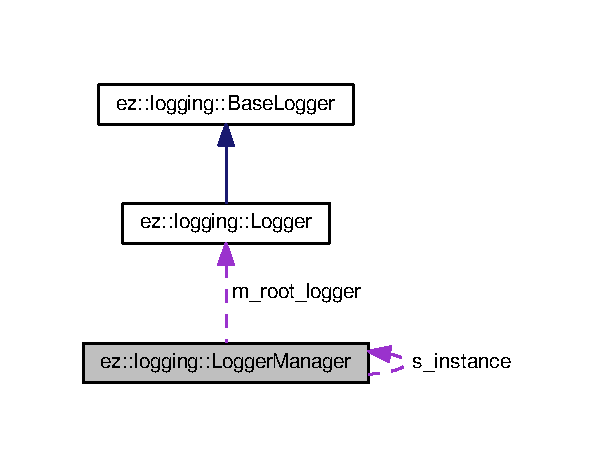
\includegraphics[width=286pt]{classez_1_1logging_1_1LoggerManager__coll__graph}
\end{center}
\end{figure}
\subsection*{Public Member Functions}
\begin{DoxyCompactItemize}
\item 
virtual \hyperlink{classez_1_1logging_1_1LoggerManager_a0738a5887eb50eba0f08a250b9aa7675}{$\sim$\+Logger\+Manager} ()
\item 
void \hyperlink{classez_1_1logging_1_1LoggerManager_a0358094fdf703ed5a5ff021fd5f94efd}{attach} (\hyperlink{classez_1_1logging_1_1Logger}{Logger} $\ast$l)
\item 
\hyperlink{classez_1_1logging_1_1Logger}{Logger} $\ast$ \hyperlink{classez_1_1logging_1_1LoggerManager_a777dcb9907e2d3cc7a314df6617ba5fb}{detach} (string name)
\item 
\hyperlink{classez_1_1logging_1_1Logger}{Logger} \& \hyperlink{classez_1_1logging_1_1LoggerManager_a90c836448bef5099d16d03b37bf52661}{get} (string name, string or\+\_\+create=\char`\"{}\char`\"{})
\item 
\hyperlink{classez_1_1logging_1_1Logger}{Logger} \& \hyperlink{classez_1_1logging_1_1LoggerManager_aa5f5fae8e256e6f3dc4269d506723b31}{root\+\_\+logger} ()
\item 
\hyperlink{classez_1_1logging_1_1Logger}{Logger} \& \hyperlink{classez_1_1logging_1_1LoggerManager_aba82648266530bd33f74d865c4c55878}{create} (string s)
\end{DoxyCompactItemize}
\subsection*{Static Public Member Functions}
\begin{DoxyCompactItemize}
\item 
static \hyperlink{classez_1_1logging_1_1LoggerManager}{Logger\+Manager} \& \hyperlink{classez_1_1logging_1_1LoggerManager_a787219c6e31bc575de95127350da7c5a}{instance} ()
\end{DoxyCompactItemize}
\subsection*{Protected Member Functions}
\begin{DoxyCompactItemize}
\item 
\hyperlink{classez_1_1logging_1_1LoggerManager_a76aa9e2191e3120990a550e064b2c691}{Logger\+Manager} ()
\end{DoxyCompactItemize}
\subsection*{Protected Attributes}
\begin{DoxyCompactItemize}
\item 
map$<$ string, \hyperlink{classez_1_1logging_1_1Logger}{Logger} $\ast$ $>$ \hyperlink{classez_1_1logging_1_1LoggerManager_a8c68f8c359e7a32438c9da137aa8b9bc}{m\+\_\+loggers}
\end{DoxyCompactItemize}
\subsection*{Static Protected Attributes}
\begin{DoxyCompactItemize}
\item 
static \hyperlink{classez_1_1logging_1_1LoggerManager}{Logger\+Manager} $\ast$ \hyperlink{classez_1_1logging_1_1LoggerManager_a635ac579d7e6e68fb248566e34d8485d}{s\+\_\+instance} = nullptr
\item 
static \hyperlink{classez_1_1logging_1_1Logger}{Logger} $\ast$ \hyperlink{classez_1_1logging_1_1LoggerManager_ac4e86e0e638673338ccb8d652446be92}{m\+\_\+root\+\_\+logger} = nullptr
\end{DoxyCompactItemize}


\subsection{Detailed Description}
\hyperlink{classez_1_1logging_1_1Logger}{Logger} Manager for the simple logging package. The role of the \hyperlink{classez_1_1logging_1_1LoggerManager}{Logger\+Manager} is to record loggers (\begin{DoxySeeAlso}{See also}
\hyperlink{classez_1_1logging_1_1Logger}{Logger}). By default a \char`\"{}root logger\char`\"{} (which is a console logger) is created. When using a logger, end line to display information by sending the \textquotesingle{}~\newline
\textquotesingle{} character or \hyperlink{classez_1_1logging_1_1Logger_a69ba6cf7130aa70caeca9f5c8636e05a}{Logger\+::endl}.
\end{DoxySeeAlso}
How to use simple logging system\+: 
\begin{DoxyItemize}
\item register new \hyperlink{classez_1_1logging_1_1ConsoleLogger}{Console\+Logger} called {\itshape stdout}\+: 
\begin{DoxyPre}{\ttfamily 
LoggerManager::get\_instance().attach(new \hyperlink{classez_1_1logging_1_1ConsoleLogger}{ConsoleLogger}("stdout", \&std::cout));
}\end{DoxyPre}
  
\item use logger {\itshape stdout}\+: 
\begin{DoxyPre}{\ttfamily 
\hyperlink{classez_1_1logging_1_1Logger}{Logger}\& log1 = \hyperlink{classez_1_1logging_1_1LoggerManager_a787219c6e31bc575de95127350da7c5a}{LoggerManager::instance()}.get\_logger("stdout");
log1 << "hello world\(\backslash\)n";
log1 << "message" << \hyperlink{classez_1_1logging_1_1Logger_a69ba6cf7130aa70caeca9f5c8636e05a}{Logger::endl};
}\end{DoxyPre}
  
\item register new \hyperlink{classez_1_1logging_1_1FileLogger}{File\+Logger} called {\itshape my}\+: 
\begin{DoxyPre}{\ttfamily 
\hyperlink{classez_1_1logging_1_1LoggerManager_a787219c6e31bc575de95127350da7c5a}{LoggerManager::instance()}.attach(new \hyperlink{classez_1_1logging_1_1FileLogger}{FileLogger}("my", "file\_logger.txt",
FileLogger::TRUNCATE));
    \hyperlink{classez_1_1logging_1_1Logger}{Logger}\& log2 = LoggerManager::get\_instance().get\_logger("my");
    }\end{DoxyPre}
  
\end{DoxyItemize}

\subsection{Constructor \& Destructor Documentation}
\mbox{\Hypertarget{classez_1_1logging_1_1LoggerManager_a0738a5887eb50eba0f08a250b9aa7675}\label{classez_1_1logging_1_1LoggerManager_a0738a5887eb50eba0f08a250b9aa7675}} 
\index{ez\+::logging\+::\+Logger\+Manager@{ez\+::logging\+::\+Logger\+Manager}!````~Logger\+Manager@{$\sim$\+Logger\+Manager}}
\index{````~Logger\+Manager@{$\sim$\+Logger\+Manager}!ez\+::logging\+::\+Logger\+Manager@{ez\+::logging\+::\+Logger\+Manager}}
\subsubsection{\texorpdfstring{$\sim$\+Logger\+Manager()}{~LoggerManager()}}
{\footnotesize\ttfamily Logger\+Manager\+::$\sim$\+Logger\+Manager (\begin{DoxyParamCaption}{ }\end{DoxyParamCaption})\hspace{0.3cm}{\ttfamily [virtual]}}

destructor that will remove all loggers \mbox{\Hypertarget{classez_1_1logging_1_1LoggerManager_a76aa9e2191e3120990a550e064b2c691}\label{classez_1_1logging_1_1LoggerManager_a76aa9e2191e3120990a550e064b2c691}} 
\index{ez\+::logging\+::\+Logger\+Manager@{ez\+::logging\+::\+Logger\+Manager}!Logger\+Manager@{Logger\+Manager}}
\index{Logger\+Manager@{Logger\+Manager}!ez\+::logging\+::\+Logger\+Manager@{ez\+::logging\+::\+Logger\+Manager}}
\subsubsection{\texorpdfstring{Logger\+Manager()}{LoggerManager()}}
{\footnotesize\ttfamily Logger\+Manager\+::\+Logger\+Manager (\begin{DoxyParamCaption}{ }\end{DoxyParamCaption})\hspace{0.3cm}{\ttfamily [protected]}}

constructor that will create a root logger 

\subsection{Member Function Documentation}
\mbox{\Hypertarget{classez_1_1logging_1_1LoggerManager_a0358094fdf703ed5a5ff021fd5f94efd}\label{classez_1_1logging_1_1LoggerManager_a0358094fdf703ed5a5ff021fd5f94efd}} 
\index{ez\+::logging\+::\+Logger\+Manager@{ez\+::logging\+::\+Logger\+Manager}!attach@{attach}}
\index{attach@{attach}!ez\+::logging\+::\+Logger\+Manager@{ez\+::logging\+::\+Logger\+Manager}}
\subsubsection{\texorpdfstring{attach()}{attach()}}
{\footnotesize\ttfamily void Logger\+Manager\+::attach (\begin{DoxyParamCaption}\item[{\hyperlink{classez_1_1logging_1_1Logger}{Logger} $\ast$}]{l }\end{DoxyParamCaption})}

add new logger, throw exception if a logger with same identifier already exists. In this case you should use the \char`\"{}get\+\_\+logger\char`\"{} method 
\begin{DoxyParams}{Parameters}
{\em l} & pointer to \hyperlink{classez_1_1logging_1_1Logger}{Logger} \\
\hline
\end{DoxyParams}
\mbox{\Hypertarget{classez_1_1logging_1_1LoggerManager_aba82648266530bd33f74d865c4c55878}\label{classez_1_1logging_1_1LoggerManager_aba82648266530bd33f74d865c4c55878}} 
\index{ez\+::logging\+::\+Logger\+Manager@{ez\+::logging\+::\+Logger\+Manager}!create@{create}}
\index{create@{create}!ez\+::logging\+::\+Logger\+Manager@{ez\+::logging\+::\+Logger\+Manager}}
\subsubsection{\texorpdfstring{create()}{create()}}
{\footnotesize\ttfamily \hyperlink{classez_1_1logging_1_1Logger}{Logger} \& Logger\+Manager\+::create (\begin{DoxyParamCaption}\item[{string}]{s }\end{DoxyParamCaption})}

create logger from string description\+: 
\begin{DoxyItemize}
\item for console logger use \char`\"{}console\char`\"{} or \char`\"{}console,stdout\char`\"{} or \char`\"{}console,stderr\char`\"{} 
\item for file logger use \char`\"{}file,name-\/of-\/file\char`\"{} or \char`\"{}file,name-\/of-\/file,truncate\char`\"{} 
\end{DoxyItemize}\mbox{\Hypertarget{classez_1_1logging_1_1LoggerManager_a777dcb9907e2d3cc7a314df6617ba5fb}\label{classez_1_1logging_1_1LoggerManager_a777dcb9907e2d3cc7a314df6617ba5fb}} 
\index{ez\+::logging\+::\+Logger\+Manager@{ez\+::logging\+::\+Logger\+Manager}!detach@{detach}}
\index{detach@{detach}!ez\+::logging\+::\+Logger\+Manager@{ez\+::logging\+::\+Logger\+Manager}}
\subsubsection{\texorpdfstring{detach()}{detach()}}
{\footnotesize\ttfamily \hyperlink{classez_1_1logging_1_1Logger}{Logger} $\ast$ Logger\+Manager\+::detach (\begin{DoxyParamCaption}\item[{string}]{name }\end{DoxyParamCaption})}

remove logger and return pointer to it. An exception will be generated if the name of the logger is not found 
\begin{DoxyParams}{Parameters}
{\em name} & identifier of \hyperlink{classez_1_1logging_1_1Logger}{Logger} \\
\hline
\end{DoxyParams}
\begin{DoxyReturn}{Returns}
pointer to \hyperlink{classez_1_1logging_1_1Logger}{Logger} 
\end{DoxyReturn}
\mbox{\Hypertarget{classez_1_1logging_1_1LoggerManager_a90c836448bef5099d16d03b37bf52661}\label{classez_1_1logging_1_1LoggerManager_a90c836448bef5099d16d03b37bf52661}} 
\index{ez\+::logging\+::\+Logger\+Manager@{ez\+::logging\+::\+Logger\+Manager}!get@{get}}
\index{get@{get}!ez\+::logging\+::\+Logger\+Manager@{ez\+::logging\+::\+Logger\+Manager}}
\subsubsection{\texorpdfstring{get()}{get()}}
{\footnotesize\ttfamily \hyperlink{classez_1_1logging_1_1Logger}{Logger} \& Logger\+Manager\+::get (\begin{DoxyParamCaption}\item[{string}]{name,  }\item[{string}]{or\+\_\+create = {\ttfamily \char`\"{}\char`\"{}} }\end{DoxyParamCaption})}

return reference to existing logger identified by its name, an exception is raised if the logger is not found 
\begin{DoxyParams}{Parameters}
{\em name} & identifier of \hyperlink{classez_1_1logging_1_1Logger}{Logger} \\
\hline
{\em or\+\_\+create} & string to create log (\\
\hline
\end{DoxyParams}
\begin{DoxySeeAlso}{See also}
\hyperlink{classez_1_1logging_1_1LoggerManager_aba82648266530bd33f74d865c4c55878}{create}) 
\end{DoxySeeAlso}
\begin{DoxyReturn}{Returns}
reference to logger if if exists or throws exception 
\end{DoxyReturn}
\mbox{\Hypertarget{classez_1_1logging_1_1LoggerManager_a787219c6e31bc575de95127350da7c5a}\label{classez_1_1logging_1_1LoggerManager_a787219c6e31bc575de95127350da7c5a}} 
\index{ez\+::logging\+::\+Logger\+Manager@{ez\+::logging\+::\+Logger\+Manager}!instance@{instance}}
\index{instance@{instance}!ez\+::logging\+::\+Logger\+Manager@{ez\+::logging\+::\+Logger\+Manager}}
\subsubsection{\texorpdfstring{instance()}{instance()}}
{\footnotesize\ttfamily \hyperlink{classez_1_1logging_1_1LoggerManager}{Logger\+Manager} \& Logger\+Manager\+::instance (\begin{DoxyParamCaption}{ }\end{DoxyParamCaption})\hspace{0.3cm}{\ttfamily [static]}}

return instance of this class \mbox{\Hypertarget{classez_1_1logging_1_1LoggerManager_aa5f5fae8e256e6f3dc4269d506723b31}\label{classez_1_1logging_1_1LoggerManager_aa5f5fae8e256e6f3dc4269d506723b31}} 
\index{ez\+::logging\+::\+Logger\+Manager@{ez\+::logging\+::\+Logger\+Manager}!root\+\_\+logger@{root\+\_\+logger}}
\index{root\+\_\+logger@{root\+\_\+logger}!ez\+::logging\+::\+Logger\+Manager@{ez\+::logging\+::\+Logger\+Manager}}
\subsubsection{\texorpdfstring{root\+\_\+logger()}{root\_logger()}}
{\footnotesize\ttfamily \hyperlink{classez_1_1logging_1_1Logger}{Logger} \& Logger\+Manager\+::root\+\_\+logger (\begin{DoxyParamCaption}{ }\end{DoxyParamCaption})}

return reference to root logger \begin{DoxyReturn}{Returns}
reference to root logger 
\end{DoxyReturn}


\subsection{Field Documentation}
\mbox{\Hypertarget{classez_1_1logging_1_1LoggerManager_a8c68f8c359e7a32438c9da137aa8b9bc}\label{classez_1_1logging_1_1LoggerManager_a8c68f8c359e7a32438c9da137aa8b9bc}} 
\index{ez\+::logging\+::\+Logger\+Manager@{ez\+::logging\+::\+Logger\+Manager}!m\+\_\+loggers@{m\+\_\+loggers}}
\index{m\+\_\+loggers@{m\+\_\+loggers}!ez\+::logging\+::\+Logger\+Manager@{ez\+::logging\+::\+Logger\+Manager}}
\subsubsection{\texorpdfstring{m\+\_\+loggers}{m\_loggers}}
{\footnotesize\ttfamily map$<$string, \hyperlink{classez_1_1logging_1_1Logger}{Logger} $\ast$$>$ ez\+::logging\+::\+Logger\+Manager\+::m\+\_\+loggers\hspace{0.3cm}{\ttfamily [protected]}}

records the loggers and their names \mbox{\Hypertarget{classez_1_1logging_1_1LoggerManager_ac4e86e0e638673338ccb8d652446be92}\label{classez_1_1logging_1_1LoggerManager_ac4e86e0e638673338ccb8d652446be92}} 
\index{ez\+::logging\+::\+Logger\+Manager@{ez\+::logging\+::\+Logger\+Manager}!m\+\_\+root\+\_\+logger@{m\+\_\+root\+\_\+logger}}
\index{m\+\_\+root\+\_\+logger@{m\+\_\+root\+\_\+logger}!ez\+::logging\+::\+Logger\+Manager@{ez\+::logging\+::\+Logger\+Manager}}
\subsubsection{\texorpdfstring{m\+\_\+root\+\_\+logger}{m\_root\_logger}}
{\footnotesize\ttfamily \hyperlink{classez_1_1logging_1_1Logger}{Logger} $\ast$ Logger\+Manager\+::m\+\_\+root\+\_\+logger = nullptr\hspace{0.3cm}{\ttfamily [static]}, {\ttfamily [protected]}}

unique instance of root logger \mbox{\Hypertarget{classez_1_1logging_1_1LoggerManager_a635ac579d7e6e68fb248566e34d8485d}\label{classez_1_1logging_1_1LoggerManager_a635ac579d7e6e68fb248566e34d8485d}} 
\index{ez\+::logging\+::\+Logger\+Manager@{ez\+::logging\+::\+Logger\+Manager}!s\+\_\+instance@{s\+\_\+instance}}
\index{s\+\_\+instance@{s\+\_\+instance}!ez\+::logging\+::\+Logger\+Manager@{ez\+::logging\+::\+Logger\+Manager}}
\subsubsection{\texorpdfstring{s\+\_\+instance}{s\_instance}}
{\footnotesize\ttfamily \hyperlink{classez_1_1logging_1_1LoggerManager}{Logger\+Manager} $\ast$ Logger\+Manager\+::s\+\_\+instance = nullptr\hspace{0.3cm}{\ttfamily [static]}, {\ttfamily [protected]}}

unique instance of \hyperlink{classez_1_1logging_1_1LoggerManager}{Logger\+Manager} 

The documentation for this class was generated from the following files\+:\begin{DoxyCompactItemize}
\item 
src/version\+\_\+2018.\+06/logging/logger\+\_\+manager.\+h\item 
src/version\+\_\+2018.\+06/logging/logger\+\_\+manager.\+cpp\end{DoxyCompactItemize}

\hypertarget{classez_1_1objects_1_1LongInteger}{}\section{ez\+:\+:objects\+:\+:Long\+Integer Class Reference}
\label{classez_1_1objects_1_1LongInteger}\index{ez\+::objects\+::\+Long\+Integer@{ez\+::objects\+::\+Long\+Integer}}


Inheritance diagram for ez\+:\+:objects\+:\+:Long\+Integer\+:
\nopagebreak
\begin{figure}[H]
\begin{center}
\leavevmode
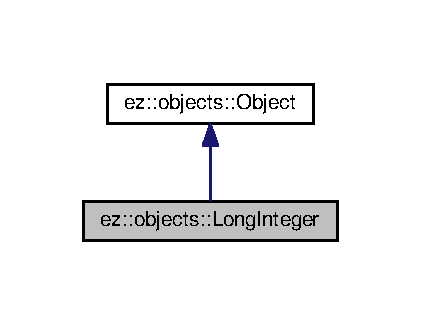
\includegraphics[width=202pt]{classez_1_1objects_1_1LongInteger__inherit__graph}
\end{center}
\end{figure}


Collaboration diagram for ez\+:\+:objects\+:\+:Long\+Integer\+:
\nopagebreak
\begin{figure}[H]
\begin{center}
\leavevmode
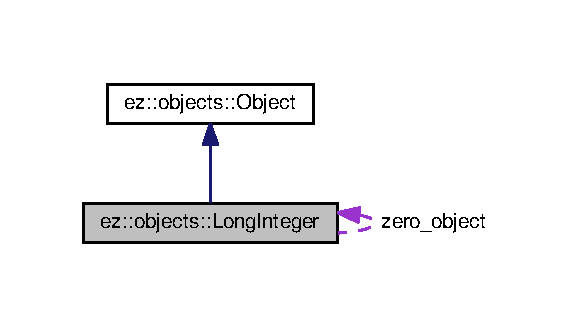
\includegraphics[width=274pt]{classez_1_1objects_1_1LongInteger__coll__graph}
\end{center}
\end{figure}
\subsection*{Public Types}
\begin{DoxyCompactItemize}
\item 
\mbox{\Hypertarget{classez_1_1objects_1_1LongInteger_a8f4d456ffd2dd99602d406bee72619d0}\label{classez_1_1objects_1_1LongInteger_a8f4d456ffd2dd99602d406bee72619d0}} 
typedef \hyperlink{classez_1_1objects_1_1LongInteger}{Long\+Integer} {\bfseries self}
\end{DoxyCompactItemize}
\subsection*{Public Member Functions}
\begin{DoxyCompactItemize}
\item 
\hyperlink{classez_1_1objects_1_1LongInteger_aabc00d94ae5a2af535316cf674c83965}{Long\+Integer} ()
\item 
\hyperlink{classez_1_1objects_1_1LongInteger_a111bbd17362b965bdfcceea9a7434204}{Long\+Integer} (integer x)
\item 
\hyperlink{classez_1_1objects_1_1LongInteger_a8cfd4cb5790eac3da3d2384f7c91a21d}{Long\+Integer} (const \hyperlink{classez_1_1objects_1_1LongInteger}{Long\+Integer} \&obj)
\item 
\hyperlink{classez_1_1objects_1_1LongInteger}{Long\+Integer} \& \hyperlink{classez_1_1objects_1_1LongInteger_a07b95e96b762d63a4b52fca7e21b8eb2}{operator=} (const \hyperlink{classez_1_1objects_1_1LongInteger}{Long\+Integer} \&obj)
\item 
\hyperlink{classez_1_1objects_1_1LongInteger_af991f863748b4a6a4561c88700235ac0}{$\sim$\+Long\+Integer} ()
\item 
\mbox{\Hypertarget{classez_1_1objects_1_1LongInteger_a528a1359d086a261f931426f516043f6}\label{classez_1_1objects_1_1LongInteger_a528a1359d086a261f931426f516043f6}} 
long\+\_\+integer {\bfseries value} ()
\item 
\mbox{\Hypertarget{classez_1_1objects_1_1LongInteger_a6e1b702ff5ce660d9278d5d10d819da5}\label{classez_1_1objects_1_1LongInteger_a6e1b702ff5ce660d9278d5d10d819da5}} 
void {\bfseries value} (long\+\_\+integer l)
\item 
void \hyperlink{classez_1_1objects_1_1LongInteger_a61530e285ac30d7890564a6cbe6bc283}{print} (std\+::ostream \&stream)
\item 
void \hyperlink{classez_1_1objects_1_1LongInteger_a9c4f7a8c3e60ab678b43f818a07540d5}{output} (std\+::ostream \&stream)
\item 
void \hyperlink{classez_1_1objects_1_1LongInteger_a9fa1d50b8d4d7e2ea2383bb625712349}{input} (std\+::istream \&stream)
\item 
\hyperlink{classez_1_1objects_1_1Object}{Object} $\ast$ \hyperlink{classez_1_1objects_1_1LongInteger_af19a10913ba906a81cdb164897edade6}{clone} ()
\item 
bool \hyperlink{classez_1_1objects_1_1LongInteger_ad9241d39b14d6cff1173c692ac37c8fc}{is\+\_\+numeric} ()
\item 
integer \hyperlink{classez_1_1objects_1_1LongInteger_ac2771a597b5f2ed611d9eb10f4339019}{compare} (const \hyperlink{classez_1_1objects_1_1Object}{Object} \&y)
\item 
long\+\_\+integer \hyperlink{classez_1_1objects_1_1LongInteger_a0b63a198b5c4e0f2a05a400788fbc8a8}{factorial} ()
\item 
\mbox{\Hypertarget{classez_1_1objects_1_1LongInteger_a9df8e14386f691b035417c6f6beca71d}\label{classez_1_1objects_1_1LongInteger_a9df8e14386f691b035417c6f6beca71d}} 
long\+\_\+integer {\bfseries fibonacci} ()
\item 
\mbox{\Hypertarget{classez_1_1objects_1_1LongInteger_af49345d7916d909c81bdf935ffa30518}\label{classez_1_1objects_1_1LongInteger_af49345d7916d909c81bdf935ffa30518}} 
long\+\_\+integer {\bfseries sqrt} ()
\item 
\mbox{\Hypertarget{classez_1_1objects_1_1LongInteger_a866072ed2beb4ac1c029d9e4c828c9b5}\label{classez_1_1objects_1_1LongInteger_a866072ed2beb4ac1c029d9e4c828c9b5}} 
bool {\bfseries is\+\_\+prime} ()
\item 
\mbox{\Hypertarget{classez_1_1objects_1_1LongInteger_a9ca5712deeddb4afa119eb5c4a6c3a10}\label{classez_1_1objects_1_1LongInteger_a9ca5712deeddb4afa119eb5c4a6c3a10}} 
\hyperlink{classez_1_1objects_1_1LongInteger}{self} \& {\bfseries operator+=} (const \hyperlink{classez_1_1objects_1_1LongInteger}{self} \&y)
\item 
\mbox{\Hypertarget{classez_1_1objects_1_1LongInteger_abd3bd1adc7a422b114a65041d94c8c57}\label{classez_1_1objects_1_1LongInteger_abd3bd1adc7a422b114a65041d94c8c57}} 
\hyperlink{classez_1_1objects_1_1LongInteger}{self} \& {\bfseries operator-\/=} (const \hyperlink{classez_1_1objects_1_1LongInteger}{self} \&y)
\item 
\mbox{\Hypertarget{classez_1_1objects_1_1LongInteger_a461b6176b9d0a48713ed6d95cdf8a3fd}\label{classez_1_1objects_1_1LongInteger_a461b6176b9d0a48713ed6d95cdf8a3fd}} 
\hyperlink{classez_1_1objects_1_1LongInteger}{self} \& {\bfseries operator/=} (const \hyperlink{classez_1_1objects_1_1LongInteger}{self} \&y)
\item 
\mbox{\Hypertarget{classez_1_1objects_1_1LongInteger_acdeee7a13e74bffa137a8ed3c5617919}\label{classez_1_1objects_1_1LongInteger_acdeee7a13e74bffa137a8ed3c5617919}} 
\hyperlink{classez_1_1objects_1_1LongInteger}{self} \& {\bfseries operator$\ast$=} (const \hyperlink{classez_1_1objects_1_1LongInteger}{self} \&y)
\item 
\mbox{\Hypertarget{classez_1_1objects_1_1LongInteger_a6c828abf40f8994a5358515264ba6bed}\label{classez_1_1objects_1_1LongInteger_a6c828abf40f8994a5358515264ba6bed}} 
\hyperlink{classez_1_1objects_1_1LongInteger}{self} \& {\bfseries operator++} ()
\item 
\mbox{\Hypertarget{classez_1_1objects_1_1LongInteger_a46ffc0a602e001c7fc9fbb04aac79322}\label{classez_1_1objects_1_1LongInteger_a46ffc0a602e001c7fc9fbb04aac79322}} 
\hyperlink{classez_1_1objects_1_1LongInteger}{self} {\bfseries operator++} (int junk)
\item 
\mbox{\Hypertarget{classez_1_1objects_1_1LongInteger_a44983751c9623ba9b9be762b050ebba9}\label{classez_1_1objects_1_1LongInteger_a44983751c9623ba9b9be762b050ebba9}} 
\hyperlink{classez_1_1objects_1_1LongInteger}{self} \& {\bfseries operator-\/-\/} ()
\item 
\mbox{\Hypertarget{classez_1_1objects_1_1LongInteger_af01529a771f55ad20575e06aa6876303}\label{classez_1_1objects_1_1LongInteger_af01529a771f55ad20575e06aa6876303}} 
\hyperlink{classez_1_1objects_1_1LongInteger}{self} {\bfseries operator-\/-\/} (int junk)
\item 
\mbox{\Hypertarget{classez_1_1objects_1_1LongInteger_a21623d2785230d246f502747cbe085b6}\label{classez_1_1objects_1_1LongInteger_a21623d2785230d246f502747cbe085b6}} 
long\+\_\+integer {\bfseries min} ()
\item 
\mbox{\Hypertarget{classez_1_1objects_1_1LongInteger_aca0bd81656855177176e11638ab8a253}\label{classez_1_1objects_1_1LongInteger_aca0bd81656855177176e11638ab8a253}} 
long\+\_\+integer {\bfseries max} ()
\end{DoxyCompactItemize}
\subsection*{Static Public Member Functions}
\begin{DoxyCompactItemize}
\item 
static long\+\_\+integer \hyperlink{classez_1_1objects_1_1LongInteger_a555e78bdf1c29fef8784e2e80ba97524}{factorial} (long\+\_\+integer x)
\item 
static long\+\_\+integer \hyperlink{classez_1_1objects_1_1LongInteger_a38a5c03d9a76cb536e5ae5a4032f49bf}{fibonacci} (long\+\_\+integer x)
\item 
static long\+\_\+integer \hyperlink{classez_1_1objects_1_1LongInteger_abd2d5eb5775cb31b475d7dd20972cfc5}{sqrt} (long\+\_\+integer x)
\item 
static bool \hyperlink{classez_1_1objects_1_1LongInteger_a7794d4a28648c4b1a4793f0498567fe3}{is\+\_\+prime} (long\+\_\+integer x)
\end{DoxyCompactItemize}
\subsection*{Data Fields}
\begin{DoxyCompactItemize}
\item 
\mbox{\Hypertarget{classez_1_1objects_1_1LongInteger_a204ed29aad25ee92509303f0768449f2}\label{classez_1_1objects_1_1LongInteger_a204ed29aad25ee92509303f0768449f2}} 
long\+\_\+integer {\bfseries m\+\_\+value}
\end{DoxyCompactItemize}
\subsection*{Static Public Attributes}
\begin{DoxyCompactItemize}
\item 
\mbox{\Hypertarget{classez_1_1objects_1_1LongInteger_a06db532fa2100af8e6c0a2d3062fa651}\label{classez_1_1objects_1_1LongInteger_a06db532fa2100af8e6c0a2d3062fa651}} 
static long\+\_\+integer {\bfseries zero} = 0
\item 
\mbox{\Hypertarget{classez_1_1objects_1_1LongInteger_aea092e1420042411ad7af704e2467b03}\label{classez_1_1objects_1_1LongInteger_aea092e1420042411ad7af704e2467b03}} 
static \hyperlink{classez_1_1objects_1_1LongInteger}{Long\+Integer} {\bfseries zero\+\_\+object}
\end{DoxyCompactItemize}
\subsection*{Friends}
\begin{DoxyCompactItemize}
\item 
\mbox{\Hypertarget{classez_1_1objects_1_1LongInteger_ac219ecb06730e7707b9bb78b5da63c3b}\label{classez_1_1objects_1_1LongInteger_ac219ecb06730e7707b9bb78b5da63c3b}} 
\hyperlink{classez_1_1objects_1_1LongInteger}{self} {\bfseries operator+} (const \hyperlink{classez_1_1objects_1_1LongInteger}{self} x, const \hyperlink{classez_1_1objects_1_1LongInteger}{self} y)
\item 
\mbox{\Hypertarget{classez_1_1objects_1_1LongInteger_a6750cba02a1d652b1bd892bfba555e50}\label{classez_1_1objects_1_1LongInteger_a6750cba02a1d652b1bd892bfba555e50}} 
\hyperlink{classez_1_1objects_1_1LongInteger}{self} {\bfseries operator-\/} (const \hyperlink{classez_1_1objects_1_1LongInteger}{self} x, const \hyperlink{classez_1_1objects_1_1LongInteger}{self} y)
\item 
\mbox{\Hypertarget{classez_1_1objects_1_1LongInteger_a4f9af882c7a074ed8e1f8da41bd31dc9}\label{classez_1_1objects_1_1LongInteger_a4f9af882c7a074ed8e1f8da41bd31dc9}} 
\hyperlink{classez_1_1objects_1_1LongInteger}{self} {\bfseries operator$\ast$} (const \hyperlink{classez_1_1objects_1_1LongInteger}{self} x, const \hyperlink{classez_1_1objects_1_1LongInteger}{self} y)
\item 
\mbox{\Hypertarget{classez_1_1objects_1_1LongInteger_aa69c5e8b6898bb99a6f4d6e8962560c8}\label{classez_1_1objects_1_1LongInteger_aa69c5e8b6898bb99a6f4d6e8962560c8}} 
\hyperlink{classez_1_1objects_1_1LongInteger}{self} {\bfseries operator/} (const \hyperlink{classez_1_1objects_1_1LongInteger}{self} x, const \hyperlink{classez_1_1objects_1_1LongInteger}{self} y)
\end{DoxyCompactItemize}


\subsection{Constructor \& Destructor Documentation}
\mbox{\Hypertarget{classez_1_1objects_1_1LongInteger_aabc00d94ae5a2af535316cf674c83965}\label{classez_1_1objects_1_1LongInteger_aabc00d94ae5a2af535316cf674c83965}} 
\index{ez\+::objects\+::\+Long\+Integer@{ez\+::objects\+::\+Long\+Integer}!Long\+Integer@{Long\+Integer}}
\index{Long\+Integer@{Long\+Integer}!ez\+::objects\+::\+Long\+Integer@{ez\+::objects\+::\+Long\+Integer}}
\subsubsection{\texorpdfstring{Long\+Integer()}{LongInteger()}\hspace{0.1cm}{\footnotesize\ttfamily [1/3]}}
{\footnotesize\ttfamily ez\+::objects\+::\+Long\+Integer\+::\+Long\+Integer (\begin{DoxyParamCaption}{ }\end{DoxyParamCaption})\hspace{0.3cm}{\ttfamily [inline]}}

default constructor \mbox{\Hypertarget{classez_1_1objects_1_1LongInteger_a111bbd17362b965bdfcceea9a7434204}\label{classez_1_1objects_1_1LongInteger_a111bbd17362b965bdfcceea9a7434204}} 
\index{ez\+::objects\+::\+Long\+Integer@{ez\+::objects\+::\+Long\+Integer}!Long\+Integer@{Long\+Integer}}
\index{Long\+Integer@{Long\+Integer}!ez\+::objects\+::\+Long\+Integer@{ez\+::objects\+::\+Long\+Integer}}
\subsubsection{\texorpdfstring{Long\+Integer()}{LongInteger()}\hspace{0.1cm}{\footnotesize\ttfamily [2/3]}}
{\footnotesize\ttfamily ez\+::objects\+::\+Long\+Integer\+::\+Long\+Integer (\begin{DoxyParamCaption}\item[{integer}]{x }\end{DoxyParamCaption})\hspace{0.3cm}{\ttfamily [inline]}}

constructor given an initial value \mbox{\Hypertarget{classez_1_1objects_1_1LongInteger_a8cfd4cb5790eac3da3d2384f7c91a21d}\label{classez_1_1objects_1_1LongInteger_a8cfd4cb5790eac3da3d2384f7c91a21d}} 
\index{ez\+::objects\+::\+Long\+Integer@{ez\+::objects\+::\+Long\+Integer}!Long\+Integer@{Long\+Integer}}
\index{Long\+Integer@{Long\+Integer}!ez\+::objects\+::\+Long\+Integer@{ez\+::objects\+::\+Long\+Integer}}
\subsubsection{\texorpdfstring{Long\+Integer()}{LongInteger()}\hspace{0.1cm}{\footnotesize\ttfamily [3/3]}}
{\footnotesize\ttfamily ez\+::objects\+::\+Long\+Integer\+::\+Long\+Integer (\begin{DoxyParamCaption}\item[{const \hyperlink{classez_1_1objects_1_1LongInteger}{Long\+Integer} \&}]{obj }\end{DoxyParamCaption})\hspace{0.3cm}{\ttfamily [inline]}}

copy constructor \mbox{\Hypertarget{classez_1_1objects_1_1LongInteger_af991f863748b4a6a4561c88700235ac0}\label{classez_1_1objects_1_1LongInteger_af991f863748b4a6a4561c88700235ac0}} 
\index{ez\+::objects\+::\+Long\+Integer@{ez\+::objects\+::\+Long\+Integer}!````~Long\+Integer@{$\sim$\+Long\+Integer}}
\index{````~Long\+Integer@{$\sim$\+Long\+Integer}!ez\+::objects\+::\+Long\+Integer@{ez\+::objects\+::\+Long\+Integer}}
\subsubsection{\texorpdfstring{$\sim$\+Long\+Integer()}{~LongInteger()}}
{\footnotesize\ttfamily ez\+::objects\+::\+Long\+Integer\+::$\sim$\+Long\+Integer (\begin{DoxyParamCaption}{ }\end{DoxyParamCaption})\hspace{0.3cm}{\ttfamily [inline]}}

destructor 

\subsection{Member Function Documentation}
\mbox{\Hypertarget{classez_1_1objects_1_1LongInteger_af19a10913ba906a81cdb164897edade6}\label{classez_1_1objects_1_1LongInteger_af19a10913ba906a81cdb164897edade6}} 
\index{ez\+::objects\+::\+Long\+Integer@{ez\+::objects\+::\+Long\+Integer}!clone@{clone}}
\index{clone@{clone}!ez\+::objects\+::\+Long\+Integer@{ez\+::objects\+::\+Long\+Integer}}
\subsubsection{\texorpdfstring{clone()}{clone()}}
{\footnotesize\ttfamily \hyperlink{classez_1_1objects_1_1Object}{Object}$\ast$ ez\+::objects\+::\+Long\+Integer\+::clone (\begin{DoxyParamCaption}{ }\end{DoxyParamCaption})\hspace{0.3cm}{\ttfamily [inline]}, {\ttfamily [virtual]}}

return a copy of the object 

Reimplemented from \hyperlink{classez_1_1objects_1_1Object_acf444b2581d898eb4b8c92c2d5865c9e}{ez\+::objects\+::\+Object}.

\mbox{\Hypertarget{classez_1_1objects_1_1LongInteger_ac2771a597b5f2ed611d9eb10f4339019}\label{classez_1_1objects_1_1LongInteger_ac2771a597b5f2ed611d9eb10f4339019}} 
\index{ez\+::objects\+::\+Long\+Integer@{ez\+::objects\+::\+Long\+Integer}!compare@{compare}}
\index{compare@{compare}!ez\+::objects\+::\+Long\+Integer@{ez\+::objects\+::\+Long\+Integer}}
\subsubsection{\texorpdfstring{compare()}{compare()}}
{\footnotesize\ttfamily integer ez\+::objects\+::\+Long\+Integer\+::compare (\begin{DoxyParamCaption}\item[{const \hyperlink{classez_1_1objects_1_1Object}{Object} \&}]{y }\end{DoxyParamCaption})\hspace{0.3cm}{\ttfamily [inline]}, {\ttfamily [virtual]}}

equality between objects 

Reimplemented from \hyperlink{classez_1_1objects_1_1Object_aca311d389dffa204e425463145f4e1e6}{ez\+::objects\+::\+Object}.

\mbox{\Hypertarget{classez_1_1objects_1_1LongInteger_a555e78bdf1c29fef8784e2e80ba97524}\label{classez_1_1objects_1_1LongInteger_a555e78bdf1c29fef8784e2e80ba97524}} 
\index{ez\+::objects\+::\+Long\+Integer@{ez\+::objects\+::\+Long\+Integer}!factorial@{factorial}}
\index{factorial@{factorial}!ez\+::objects\+::\+Long\+Integer@{ez\+::objects\+::\+Long\+Integer}}
\subsubsection{\texorpdfstring{factorial()}{factorial()}\hspace{0.1cm}{\footnotesize\ttfamily [1/2]}}
{\footnotesize\ttfamily long\+\_\+integer Long\+Integer\+::factorial (\begin{DoxyParamCaption}\item[{long\+\_\+integer}]{x }\end{DoxyParamCaption})\hspace{0.3cm}{\ttfamily [static]}}

compute factorial of an \hyperlink{classez_1_1objects_1_1Integer}{Integer} \mbox{\Hypertarget{classez_1_1objects_1_1LongInteger_a0b63a198b5c4e0f2a05a400788fbc8a8}\label{classez_1_1objects_1_1LongInteger_a0b63a198b5c4e0f2a05a400788fbc8a8}} 
\index{ez\+::objects\+::\+Long\+Integer@{ez\+::objects\+::\+Long\+Integer}!factorial@{factorial}}
\index{factorial@{factorial}!ez\+::objects\+::\+Long\+Integer@{ez\+::objects\+::\+Long\+Integer}}
\subsubsection{\texorpdfstring{factorial()}{factorial()}\hspace{0.1cm}{\footnotesize\ttfamily [2/2]}}
{\footnotesize\ttfamily long\+\_\+integer ez\+::objects\+::\+Long\+Integer\+::factorial (\begin{DoxyParamCaption}{ }\end{DoxyParamCaption})\hspace{0.3cm}{\ttfamily [inline]}}

compute factorial of this \hyperlink{classez_1_1objects_1_1Integer}{Integer} \begin{DoxyReturn}{Returns}
factorial is in allowed range of values 
\end{DoxyReturn}
\mbox{\Hypertarget{classez_1_1objects_1_1LongInteger_a38a5c03d9a76cb536e5ae5a4032f49bf}\label{classez_1_1objects_1_1LongInteger_a38a5c03d9a76cb536e5ae5a4032f49bf}} 
\index{ez\+::objects\+::\+Long\+Integer@{ez\+::objects\+::\+Long\+Integer}!fibonacci@{fibonacci}}
\index{fibonacci@{fibonacci}!ez\+::objects\+::\+Long\+Integer@{ez\+::objects\+::\+Long\+Integer}}
\subsubsection{\texorpdfstring{fibonacci()}{fibonacci()}}
{\footnotesize\ttfamily long\+\_\+integer Long\+Integer\+::fibonacci (\begin{DoxyParamCaption}\item[{long\+\_\+integer}]{x }\end{DoxyParamCaption})\hspace{0.3cm}{\ttfamily [static]}}

compute fibonacci of an \hyperlink{classez_1_1objects_1_1Integer}{Integer} \mbox{\Hypertarget{classez_1_1objects_1_1LongInteger_a9fa1d50b8d4d7e2ea2383bb625712349}\label{classez_1_1objects_1_1LongInteger_a9fa1d50b8d4d7e2ea2383bb625712349}} 
\index{ez\+::objects\+::\+Long\+Integer@{ez\+::objects\+::\+Long\+Integer}!input@{input}}
\index{input@{input}!ez\+::objects\+::\+Long\+Integer@{ez\+::objects\+::\+Long\+Integer}}
\subsubsection{\texorpdfstring{input()}{input()}}
{\footnotesize\ttfamily void Long\+Integer\+::input (\begin{DoxyParamCaption}\item[{std\+::istream \&}]{stream }\end{DoxyParamCaption})\hspace{0.3cm}{\ttfamily [virtual]}}

this function is used to get the data field members of an object from a stream and acts as unserialize 

Reimplemented from \hyperlink{classez_1_1objects_1_1Object_a878bdc53b7f16fda6fa15dab214c4b6a}{ez\+::objects\+::\+Object}.

\mbox{\Hypertarget{classez_1_1objects_1_1LongInteger_ad9241d39b14d6cff1173c692ac37c8fc}\label{classez_1_1objects_1_1LongInteger_ad9241d39b14d6cff1173c692ac37c8fc}} 
\index{ez\+::objects\+::\+Long\+Integer@{ez\+::objects\+::\+Long\+Integer}!is\+\_\+numeric@{is\+\_\+numeric}}
\index{is\+\_\+numeric@{is\+\_\+numeric}!ez\+::objects\+::\+Long\+Integer@{ez\+::objects\+::\+Long\+Integer}}
\subsubsection{\texorpdfstring{is\+\_\+numeric()}{is\_numeric()}}
{\footnotesize\ttfamily bool ez\+::objects\+::\+Long\+Integer\+::is\+\_\+numeric (\begin{DoxyParamCaption}{ }\end{DoxyParamCaption})\hspace{0.3cm}{\ttfamily [inline]}, {\ttfamily [virtual]}}

indicates if this object can be used for computation 

Reimplemented from \hyperlink{classez_1_1objects_1_1Object_a19ba1672d4063232c4619e016ca178f8}{ez\+::objects\+::\+Object}.

\mbox{\Hypertarget{classez_1_1objects_1_1LongInteger_a7794d4a28648c4b1a4793f0498567fe3}\label{classez_1_1objects_1_1LongInteger_a7794d4a28648c4b1a4793f0498567fe3}} 
\index{ez\+::objects\+::\+Long\+Integer@{ez\+::objects\+::\+Long\+Integer}!is\+\_\+prime@{is\+\_\+prime}}
\index{is\+\_\+prime@{is\+\_\+prime}!ez\+::objects\+::\+Long\+Integer@{ez\+::objects\+::\+Long\+Integer}}
\subsubsection{\texorpdfstring{is\+\_\+prime()}{is\_prime()}}
{\footnotesize\ttfamily bool Long\+Integer\+::is\+\_\+prime (\begin{DoxyParamCaption}\item[{long\+\_\+integer}]{x }\end{DoxyParamCaption})\hspace{0.3cm}{\ttfamily [static]}}

check if given integer x is prime \begin{DoxyReturn}{Returns}
true if x is a prime number 
\end{DoxyReturn}
\mbox{\Hypertarget{classez_1_1objects_1_1LongInteger_a07b95e96b762d63a4b52fca7e21b8eb2}\label{classez_1_1objects_1_1LongInteger_a07b95e96b762d63a4b52fca7e21b8eb2}} 
\index{ez\+::objects\+::\+Long\+Integer@{ez\+::objects\+::\+Long\+Integer}!operator=@{operator=}}
\index{operator=@{operator=}!ez\+::objects\+::\+Long\+Integer@{ez\+::objects\+::\+Long\+Integer}}
\subsubsection{\texorpdfstring{operator=()}{operator=()}}
{\footnotesize\ttfamily \hyperlink{classez_1_1objects_1_1LongInteger}{Long\+Integer}\& ez\+::objects\+::\+Long\+Integer\+::operator= (\begin{DoxyParamCaption}\item[{const \hyperlink{classez_1_1objects_1_1LongInteger}{Long\+Integer} \&}]{obj }\end{DoxyParamCaption})\hspace{0.3cm}{\ttfamily [inline]}}

assignment operator \mbox{\Hypertarget{classez_1_1objects_1_1LongInteger_a9c4f7a8c3e60ab678b43f818a07540d5}\label{classez_1_1objects_1_1LongInteger_a9c4f7a8c3e60ab678b43f818a07540d5}} 
\index{ez\+::objects\+::\+Long\+Integer@{ez\+::objects\+::\+Long\+Integer}!output@{output}}
\index{output@{output}!ez\+::objects\+::\+Long\+Integer@{ez\+::objects\+::\+Long\+Integer}}
\subsubsection{\texorpdfstring{output()}{output()}}
{\footnotesize\ttfamily void Long\+Integer\+::output (\begin{DoxyParamCaption}\item[{std\+::ostream \&}]{stream }\end{DoxyParamCaption})\hspace{0.3cm}{\ttfamily [virtual]}}

this function is used to print the contents of the object in a serializable manner 

Reimplemented from \hyperlink{classez_1_1objects_1_1Object_a0fdfe18e6c35d6b0d7e7a01265aded15}{ez\+::objects\+::\+Object}.

\mbox{\Hypertarget{classez_1_1objects_1_1LongInteger_a61530e285ac30d7890564a6cbe6bc283}\label{classez_1_1objects_1_1LongInteger_a61530e285ac30d7890564a6cbe6bc283}} 
\index{ez\+::objects\+::\+Long\+Integer@{ez\+::objects\+::\+Long\+Integer}!print@{print}}
\index{print@{print}!ez\+::objects\+::\+Long\+Integer@{ez\+::objects\+::\+Long\+Integer}}
\subsubsection{\texorpdfstring{print()}{print()}}
{\footnotesize\ttfamily void Long\+Integer\+::print (\begin{DoxyParamCaption}\item[{std\+::ostream \&}]{stream }\end{DoxyParamCaption})\hspace{0.3cm}{\ttfamily [virtual]}}

this function is used to print the contents of the object in a human readable format 
\begin{DoxyParams}{Parameters}
{\em stream} & output stream for example std\+::cout \\
\hline
\end{DoxyParams}


Reimplemented from \hyperlink{classez_1_1objects_1_1Object_a9e20f39a78163f67f000576149d858b3}{ez\+::objects\+::\+Object}.

\mbox{\Hypertarget{classez_1_1objects_1_1LongInteger_abd2d5eb5775cb31b475d7dd20972cfc5}\label{classez_1_1objects_1_1LongInteger_abd2d5eb5775cb31b475d7dd20972cfc5}} 
\index{ez\+::objects\+::\+Long\+Integer@{ez\+::objects\+::\+Long\+Integer}!sqrt@{sqrt}}
\index{sqrt@{sqrt}!ez\+::objects\+::\+Long\+Integer@{ez\+::objects\+::\+Long\+Integer}}
\subsubsection{\texorpdfstring{sqrt()}{sqrt()}}
{\footnotesize\ttfamily long\+\_\+integer Long\+Integer\+::sqrt (\begin{DoxyParamCaption}\item[{long\+\_\+integer}]{x }\end{DoxyParamCaption})\hspace{0.3cm}{\ttfamily [static]}}

compute square root of a \hyperlink{classez_1_1objects_1_1LongInteger}{Long\+Integer}. The value is rounded to the nearest integer 

The documentation for this class was generated from the following files\+:\begin{DoxyCompactItemize}
\item 
src/version\+\_\+2018.\+06/objects/long\+\_\+integer.\+h\item 
src/version\+\_\+2018.\+06/objects/long\+\_\+integer.\+cpp\end{DoxyCompactItemize}

\hypertarget{classez_1_1objects_1_1LongNatural}{}\section{ez\+:\+:objects\+:\+:Long\+Natural Class Reference}
\label{classez_1_1objects_1_1LongNatural}\index{ez\+::objects\+::\+Long\+Natural@{ez\+::objects\+::\+Long\+Natural}}


{\ttfamily \#include $<$long\+\_\+natural.\+h$>$}



Inheritance diagram for ez\+:\+:objects\+:\+:Long\+Natural\+:
\nopagebreak
\begin{figure}[H]
\begin{center}
\leavevmode
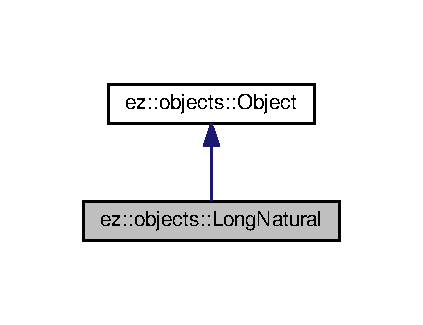
\includegraphics[width=203pt]{classez_1_1objects_1_1LongNatural__inherit__graph}
\end{center}
\end{figure}


Collaboration diagram for ez\+:\+:objects\+:\+:Long\+Natural\+:
\nopagebreak
\begin{figure}[H]
\begin{center}
\leavevmode
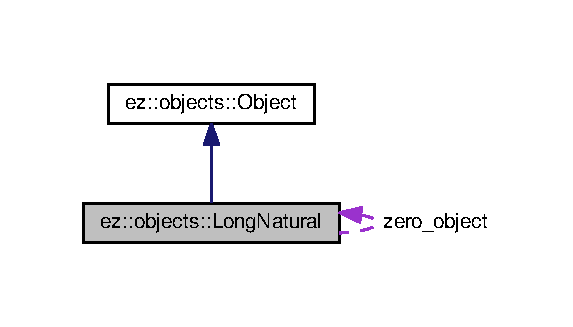
\includegraphics[width=275pt]{classez_1_1objects_1_1LongNatural__coll__graph}
\end{center}
\end{figure}
\subsection*{Public Types}
\begin{DoxyCompactItemize}
\item 
\mbox{\Hypertarget{classez_1_1objects_1_1LongNatural_ad1207a30d52155737cbaec52d3a0ab6b}\label{classez_1_1objects_1_1LongNatural_ad1207a30d52155737cbaec52d3a0ab6b}} 
typedef \hyperlink{classez_1_1objects_1_1LongNatural}{Long\+Natural} {\bfseries self}
\end{DoxyCompactItemize}
\subsection*{Public Member Functions}
\begin{DoxyCompactItemize}
\item 
\hyperlink{classez_1_1objects_1_1LongNatural_a468b880a237b7dec2051986414e809b6}{Long\+Natural} ()
\item 
\hyperlink{classez_1_1objects_1_1LongNatural_a2eef9e11dbefe9e58d53190d9eb5af45}{Long\+Natural} (natural x)
\item 
\hyperlink{classez_1_1objects_1_1LongNatural_a5c00d4b026685010514b29a962736b23}{Long\+Natural} (const \hyperlink{classez_1_1objects_1_1LongNatural}{Long\+Natural} \&obj)
\item 
\hyperlink{classez_1_1objects_1_1LongNatural}{Long\+Natural} \& \hyperlink{classez_1_1objects_1_1LongNatural_a9622a9ce2b56127a5dfbd34ca00c44cf}{operator=} (const \hyperlink{classez_1_1objects_1_1LongNatural}{Long\+Natural} \&obj)
\item 
\hyperlink{classez_1_1objects_1_1LongNatural_a551123aa83bb4cee02aca5cc9137fe45}{$\sim$\+Long\+Natural} ()
\item 
\mbox{\Hypertarget{classez_1_1objects_1_1LongNatural_a8a904d052ba54e9afebc087f31d2e23a}\label{classez_1_1objects_1_1LongNatural_a8a904d052ba54e9afebc087f31d2e23a}} 
natural {\bfseries value} ()
\item 
\mbox{\Hypertarget{classez_1_1objects_1_1LongNatural_abb0641353058618d9098c5c6c95a5204}\label{classez_1_1objects_1_1LongNatural_abb0641353058618d9098c5c6c95a5204}} 
void {\bfseries value} (natural n)
\item 
void \hyperlink{classez_1_1objects_1_1LongNatural_a38b758c27edf31447f3bc65228900266}{print} (std\+::ostream \&stream)
\item 
void \hyperlink{classez_1_1objects_1_1LongNatural_aae2570f931064a354df5553fd4425b90}{output} (std\+::ostream \&stream)
\item 
void \hyperlink{classez_1_1objects_1_1LongNatural_a37f51f88e9b039b5b59d0392ca03eeb0}{input} (std\+::istream \&stream)
\item 
\hyperlink{classez_1_1objects_1_1Object}{Object} $\ast$ \hyperlink{classez_1_1objects_1_1LongNatural_a328f33f3435bae79bbb3e9b0dcb8a3a7}{clone} ()
\item 
bool \hyperlink{classez_1_1objects_1_1LongNatural_a4cd663dc6f1eff09b83d19d76dd503cb}{is\+\_\+numeric} ()
\item 
integer \hyperlink{classez_1_1objects_1_1LongNatural_ad2ed144e5ee01a72eff476141c6e39ae}{compare} (const \hyperlink{classez_1_1objects_1_1Object}{Object} \&y)
\item 
natural \hyperlink{classez_1_1objects_1_1LongNatural_a58617d773cbbfad2a484fd7606972380}{factorial} ()
\item 
\mbox{\Hypertarget{classez_1_1objects_1_1LongNatural_a764d79ad14c17f8a9ae2932bfc24e7bd}\label{classez_1_1objects_1_1LongNatural_a764d79ad14c17f8a9ae2932bfc24e7bd}} 
natural {\bfseries fibonacci} ()
\item 
\mbox{\Hypertarget{classez_1_1objects_1_1LongNatural_aa71d01cc1ceddaab21520b363d69d302}\label{classez_1_1objects_1_1LongNatural_aa71d01cc1ceddaab21520b363d69d302}} 
natural {\bfseries sqrt} ()
\item 
\mbox{\Hypertarget{classez_1_1objects_1_1LongNatural_a9e4d0912fd93999aa18510ef55149345}\label{classez_1_1objects_1_1LongNatural_a9e4d0912fd93999aa18510ef55149345}} 
bool {\bfseries is\+\_\+prime} ()
\item 
\mbox{\Hypertarget{classez_1_1objects_1_1LongNatural_adc90aa9ee693a37f10ecb97c6b29852a}\label{classez_1_1objects_1_1LongNatural_adc90aa9ee693a37f10ecb97c6b29852a}} 
\hyperlink{classez_1_1objects_1_1LongNatural}{self} \& {\bfseries operator+=} (const \hyperlink{classez_1_1objects_1_1LongNatural}{self} \&y)
\item 
\mbox{\Hypertarget{classez_1_1objects_1_1LongNatural_a625ac512918c5a9ba4f26b0ca35ef2ac}\label{classez_1_1objects_1_1LongNatural_a625ac512918c5a9ba4f26b0ca35ef2ac}} 
\hyperlink{classez_1_1objects_1_1LongNatural}{self} \& {\bfseries operator-\/=} (const \hyperlink{classez_1_1objects_1_1LongNatural}{self} \&y)
\item 
\mbox{\Hypertarget{classez_1_1objects_1_1LongNatural_a1dae83e240d9f53183fc2ce25e5b3730}\label{classez_1_1objects_1_1LongNatural_a1dae83e240d9f53183fc2ce25e5b3730}} 
\hyperlink{classez_1_1objects_1_1LongNatural}{self} \& {\bfseries operator/=} (const \hyperlink{classez_1_1objects_1_1LongNatural}{self} \&y)
\item 
\mbox{\Hypertarget{classez_1_1objects_1_1LongNatural_a8d72970afefd2cf58458021fc737a67f}\label{classez_1_1objects_1_1LongNatural_a8d72970afefd2cf58458021fc737a67f}} 
\hyperlink{classez_1_1objects_1_1LongNatural}{self} \& {\bfseries operator$\ast$=} (const \hyperlink{classez_1_1objects_1_1LongNatural}{self} \&y)
\item 
\mbox{\Hypertarget{classez_1_1objects_1_1LongNatural_a5eba96457eaf204d1b20959d4f390d90}\label{classez_1_1objects_1_1LongNatural_a5eba96457eaf204d1b20959d4f390d90}} 
\hyperlink{classez_1_1objects_1_1LongNatural}{self} \& {\bfseries operator++} ()
\item 
\mbox{\Hypertarget{classez_1_1objects_1_1LongNatural_a57bd20a187e5a6a24bc40f28452cc0f8}\label{classez_1_1objects_1_1LongNatural_a57bd20a187e5a6a24bc40f28452cc0f8}} 
\hyperlink{classez_1_1objects_1_1LongNatural}{self} {\bfseries operator++} (int junk)
\item 
\mbox{\Hypertarget{classez_1_1objects_1_1LongNatural_a16bc2c7859534604b781fd1e57b9a47e}\label{classez_1_1objects_1_1LongNatural_a16bc2c7859534604b781fd1e57b9a47e}} 
\hyperlink{classez_1_1objects_1_1LongNatural}{self} \& {\bfseries operator-\/-\/} ()
\item 
\mbox{\Hypertarget{classez_1_1objects_1_1LongNatural_a902cc0522b5ef0a8840a5e992b27df5c}\label{classez_1_1objects_1_1LongNatural_a902cc0522b5ef0a8840a5e992b27df5c}} 
\hyperlink{classez_1_1objects_1_1LongNatural}{self} {\bfseries operator-\/-\/} (int junk)
\end{DoxyCompactItemize}
\subsection*{Static Public Member Functions}
\begin{DoxyCompactItemize}
\item 
static natural \hyperlink{classez_1_1objects_1_1LongNatural_ae67669fc6851a64143eeab0bc14deae2}{factorial} (natural x)
\item 
static natural \hyperlink{classez_1_1objects_1_1LongNatural_a40705497507f5ba97adcbd4be3ee9c19}{fibonacci} (natural x)
\item 
static natural \hyperlink{classez_1_1objects_1_1LongNatural_a70ac1efa09825aa1bde059bb176b2cb1}{sqrt} (natural x)
\item 
static bool \hyperlink{classez_1_1objects_1_1LongNatural_a87d9ed5aed5696e77a6776989b39437a}{is\+\_\+prime} (natural x)
\end{DoxyCompactItemize}
\subsection*{Data Fields}
\begin{DoxyCompactItemize}
\item 
natural \hyperlink{classez_1_1objects_1_1LongNatural_a0f7e791901688eb6067b6edb82244989}{m\+\_\+value}
\end{DoxyCompactItemize}
\subsection*{Static Public Attributes}
\begin{DoxyCompactItemize}
\item 
static natural \hyperlink{classez_1_1objects_1_1LongNatural_a86d552aacb841cd40f43da3aa3bb78e3}{zero} = 0
\item 
static \hyperlink{classez_1_1objects_1_1LongNatural}{Long\+Natural} \hyperlink{classez_1_1objects_1_1LongNatural_aac7c3b61859bd9a941b1d408f3e2e67d}{zero\+\_\+object}
\end{DoxyCompactItemize}
\subsection*{Friends}
\begin{DoxyCompactItemize}
\item 
\mbox{\Hypertarget{classez_1_1objects_1_1LongNatural_ac219ecb06730e7707b9bb78b5da63c3b}\label{classez_1_1objects_1_1LongNatural_ac219ecb06730e7707b9bb78b5da63c3b}} 
\hyperlink{classez_1_1objects_1_1LongNatural}{self} {\bfseries operator+} (const \hyperlink{classez_1_1objects_1_1LongNatural}{self} x, const \hyperlink{classez_1_1objects_1_1LongNatural}{self} y)
\item 
\mbox{\Hypertarget{classez_1_1objects_1_1LongNatural_a6750cba02a1d652b1bd892bfba555e50}\label{classez_1_1objects_1_1LongNatural_a6750cba02a1d652b1bd892bfba555e50}} 
\hyperlink{classez_1_1objects_1_1LongNatural}{self} {\bfseries operator-\/} (const \hyperlink{classez_1_1objects_1_1LongNatural}{self} x, const \hyperlink{classez_1_1objects_1_1LongNatural}{self} y)
\item 
\mbox{\Hypertarget{classez_1_1objects_1_1LongNatural_a4f9af882c7a074ed8e1f8da41bd31dc9}\label{classez_1_1objects_1_1LongNatural_a4f9af882c7a074ed8e1f8da41bd31dc9}} 
\hyperlink{classez_1_1objects_1_1LongNatural}{self} {\bfseries operator$\ast$} (const \hyperlink{classez_1_1objects_1_1LongNatural}{self} x, const \hyperlink{classez_1_1objects_1_1LongNatural}{self} y)
\item 
\mbox{\Hypertarget{classez_1_1objects_1_1LongNatural_aa69c5e8b6898bb99a6f4d6e8962560c8}\label{classez_1_1objects_1_1LongNatural_aa69c5e8b6898bb99a6f4d6e8962560c8}} 
\hyperlink{classez_1_1objects_1_1LongNatural}{self} {\bfseries operator/} (const \hyperlink{classez_1_1objects_1_1LongNatural}{self} x, const \hyperlink{classez_1_1objects_1_1LongNatural}{self} y)
\end{DoxyCompactItemize}


\subsection{Detailed Description}
Class used to represent a natural 

\subsection{Constructor \& Destructor Documentation}
\mbox{\Hypertarget{classez_1_1objects_1_1LongNatural_a468b880a237b7dec2051986414e809b6}\label{classez_1_1objects_1_1LongNatural_a468b880a237b7dec2051986414e809b6}} 
\index{ez\+::objects\+::\+Long\+Natural@{ez\+::objects\+::\+Long\+Natural}!Long\+Natural@{Long\+Natural}}
\index{Long\+Natural@{Long\+Natural}!ez\+::objects\+::\+Long\+Natural@{ez\+::objects\+::\+Long\+Natural}}
\subsubsection{\texorpdfstring{Long\+Natural()}{LongNatural()}\hspace{0.1cm}{\footnotesize\ttfamily [1/3]}}
{\footnotesize\ttfamily ez\+::objects\+::\+Long\+Natural\+::\+Long\+Natural (\begin{DoxyParamCaption}{ }\end{DoxyParamCaption})\hspace{0.3cm}{\ttfamily [inline]}}

default constructor \mbox{\Hypertarget{classez_1_1objects_1_1LongNatural_a2eef9e11dbefe9e58d53190d9eb5af45}\label{classez_1_1objects_1_1LongNatural_a2eef9e11dbefe9e58d53190d9eb5af45}} 
\index{ez\+::objects\+::\+Long\+Natural@{ez\+::objects\+::\+Long\+Natural}!Long\+Natural@{Long\+Natural}}
\index{Long\+Natural@{Long\+Natural}!ez\+::objects\+::\+Long\+Natural@{ez\+::objects\+::\+Long\+Natural}}
\subsubsection{\texorpdfstring{Long\+Natural()}{LongNatural()}\hspace{0.1cm}{\footnotesize\ttfamily [2/3]}}
{\footnotesize\ttfamily ez\+::objects\+::\+Long\+Natural\+::\+Long\+Natural (\begin{DoxyParamCaption}\item[{natural}]{x }\end{DoxyParamCaption})\hspace{0.3cm}{\ttfamily [inline]}}

constructor given an initial value \mbox{\Hypertarget{classez_1_1objects_1_1LongNatural_a5c00d4b026685010514b29a962736b23}\label{classez_1_1objects_1_1LongNatural_a5c00d4b026685010514b29a962736b23}} 
\index{ez\+::objects\+::\+Long\+Natural@{ez\+::objects\+::\+Long\+Natural}!Long\+Natural@{Long\+Natural}}
\index{Long\+Natural@{Long\+Natural}!ez\+::objects\+::\+Long\+Natural@{ez\+::objects\+::\+Long\+Natural}}
\subsubsection{\texorpdfstring{Long\+Natural()}{LongNatural()}\hspace{0.1cm}{\footnotesize\ttfamily [3/3]}}
{\footnotesize\ttfamily ez\+::objects\+::\+Long\+Natural\+::\+Long\+Natural (\begin{DoxyParamCaption}\item[{const \hyperlink{classez_1_1objects_1_1LongNatural}{Long\+Natural} \&}]{obj }\end{DoxyParamCaption})\hspace{0.3cm}{\ttfamily [inline]}}

copy constructor \mbox{\Hypertarget{classez_1_1objects_1_1LongNatural_a551123aa83bb4cee02aca5cc9137fe45}\label{classez_1_1objects_1_1LongNatural_a551123aa83bb4cee02aca5cc9137fe45}} 
\index{ez\+::objects\+::\+Long\+Natural@{ez\+::objects\+::\+Long\+Natural}!````~Long\+Natural@{$\sim$\+Long\+Natural}}
\index{````~Long\+Natural@{$\sim$\+Long\+Natural}!ez\+::objects\+::\+Long\+Natural@{ez\+::objects\+::\+Long\+Natural}}
\subsubsection{\texorpdfstring{$\sim$\+Long\+Natural()}{~LongNatural()}}
{\footnotesize\ttfamily ez\+::objects\+::\+Long\+Natural\+::$\sim$\+Long\+Natural (\begin{DoxyParamCaption}{ }\end{DoxyParamCaption})\hspace{0.3cm}{\ttfamily [inline]}}

destructor 

\subsection{Member Function Documentation}
\mbox{\Hypertarget{classez_1_1objects_1_1LongNatural_a328f33f3435bae79bbb3e9b0dcb8a3a7}\label{classez_1_1objects_1_1LongNatural_a328f33f3435bae79bbb3e9b0dcb8a3a7}} 
\index{ez\+::objects\+::\+Long\+Natural@{ez\+::objects\+::\+Long\+Natural}!clone@{clone}}
\index{clone@{clone}!ez\+::objects\+::\+Long\+Natural@{ez\+::objects\+::\+Long\+Natural}}
\subsubsection{\texorpdfstring{clone()}{clone()}}
{\footnotesize\ttfamily \hyperlink{classez_1_1objects_1_1Object}{Object}$\ast$ ez\+::objects\+::\+Long\+Natural\+::clone (\begin{DoxyParamCaption}{ }\end{DoxyParamCaption})\hspace{0.3cm}{\ttfamily [inline]}, {\ttfamily [virtual]}}

return a copy of the object 

Reimplemented from \hyperlink{classez_1_1objects_1_1Object_acf444b2581d898eb4b8c92c2d5865c9e}{ez\+::objects\+::\+Object}.

\mbox{\Hypertarget{classez_1_1objects_1_1LongNatural_ad2ed144e5ee01a72eff476141c6e39ae}\label{classez_1_1objects_1_1LongNatural_ad2ed144e5ee01a72eff476141c6e39ae}} 
\index{ez\+::objects\+::\+Long\+Natural@{ez\+::objects\+::\+Long\+Natural}!compare@{compare}}
\index{compare@{compare}!ez\+::objects\+::\+Long\+Natural@{ez\+::objects\+::\+Long\+Natural}}
\subsubsection{\texorpdfstring{compare()}{compare()}}
{\footnotesize\ttfamily integer ez\+::objects\+::\+Long\+Natural\+::compare (\begin{DoxyParamCaption}\item[{const \hyperlink{classez_1_1objects_1_1Object}{Object} \&}]{y }\end{DoxyParamCaption})\hspace{0.3cm}{\ttfamily [inline]}, {\ttfamily [virtual]}}

equality between objects 

Reimplemented from \hyperlink{classez_1_1objects_1_1Object_aca311d389dffa204e425463145f4e1e6}{ez\+::objects\+::\+Object}.

\mbox{\Hypertarget{classez_1_1objects_1_1LongNatural_ae67669fc6851a64143eeab0bc14deae2}\label{classez_1_1objects_1_1LongNatural_ae67669fc6851a64143eeab0bc14deae2}} 
\index{ez\+::objects\+::\+Long\+Natural@{ez\+::objects\+::\+Long\+Natural}!factorial@{factorial}}
\index{factorial@{factorial}!ez\+::objects\+::\+Long\+Natural@{ez\+::objects\+::\+Long\+Natural}}
\subsubsection{\texorpdfstring{factorial()}{factorial()}\hspace{0.1cm}{\footnotesize\ttfamily [1/2]}}
{\footnotesize\ttfamily natural Long\+Natural\+::factorial (\begin{DoxyParamCaption}\item[{natural}]{x }\end{DoxyParamCaption})\hspace{0.3cm}{\ttfamily [static]}}

compute factorial of an \hyperlink{classez_1_1objects_1_1Integer}{Integer} \mbox{\Hypertarget{classez_1_1objects_1_1LongNatural_a58617d773cbbfad2a484fd7606972380}\label{classez_1_1objects_1_1LongNatural_a58617d773cbbfad2a484fd7606972380}} 
\index{ez\+::objects\+::\+Long\+Natural@{ez\+::objects\+::\+Long\+Natural}!factorial@{factorial}}
\index{factorial@{factorial}!ez\+::objects\+::\+Long\+Natural@{ez\+::objects\+::\+Long\+Natural}}
\subsubsection{\texorpdfstring{factorial()}{factorial()}\hspace{0.1cm}{\footnotesize\ttfamily [2/2]}}
{\footnotesize\ttfamily natural ez\+::objects\+::\+Long\+Natural\+::factorial (\begin{DoxyParamCaption}{ }\end{DoxyParamCaption})\hspace{0.3cm}{\ttfamily [inline]}}

compute factorial of this \hyperlink{classez_1_1objects_1_1Integer}{Integer} \begin{DoxyReturn}{Returns}
factorial is in allowed range of values 
\end{DoxyReturn}
\mbox{\Hypertarget{classez_1_1objects_1_1LongNatural_a40705497507f5ba97adcbd4be3ee9c19}\label{classez_1_1objects_1_1LongNatural_a40705497507f5ba97adcbd4be3ee9c19}} 
\index{ez\+::objects\+::\+Long\+Natural@{ez\+::objects\+::\+Long\+Natural}!fibonacci@{fibonacci}}
\index{fibonacci@{fibonacci}!ez\+::objects\+::\+Long\+Natural@{ez\+::objects\+::\+Long\+Natural}}
\subsubsection{\texorpdfstring{fibonacci()}{fibonacci()}}
{\footnotesize\ttfamily natural Long\+Natural\+::fibonacci (\begin{DoxyParamCaption}\item[{natural}]{x }\end{DoxyParamCaption})\hspace{0.3cm}{\ttfamily [static]}}

compute fibonacci of an \hyperlink{classez_1_1objects_1_1Integer}{Integer} \mbox{\Hypertarget{classez_1_1objects_1_1LongNatural_a37f51f88e9b039b5b59d0392ca03eeb0}\label{classez_1_1objects_1_1LongNatural_a37f51f88e9b039b5b59d0392ca03eeb0}} 
\index{ez\+::objects\+::\+Long\+Natural@{ez\+::objects\+::\+Long\+Natural}!input@{input}}
\index{input@{input}!ez\+::objects\+::\+Long\+Natural@{ez\+::objects\+::\+Long\+Natural}}
\subsubsection{\texorpdfstring{input()}{input()}}
{\footnotesize\ttfamily void Long\+Natural\+::input (\begin{DoxyParamCaption}\item[{std\+::istream \&}]{stream }\end{DoxyParamCaption})\hspace{0.3cm}{\ttfamily [virtual]}}

this function is used to get the data field members of an object from a stream and acts as unserialize 

Reimplemented from \hyperlink{classez_1_1objects_1_1Object_a878bdc53b7f16fda6fa15dab214c4b6a}{ez\+::objects\+::\+Object}.

\mbox{\Hypertarget{classez_1_1objects_1_1LongNatural_a4cd663dc6f1eff09b83d19d76dd503cb}\label{classez_1_1objects_1_1LongNatural_a4cd663dc6f1eff09b83d19d76dd503cb}} 
\index{ez\+::objects\+::\+Long\+Natural@{ez\+::objects\+::\+Long\+Natural}!is\+\_\+numeric@{is\+\_\+numeric}}
\index{is\+\_\+numeric@{is\+\_\+numeric}!ez\+::objects\+::\+Long\+Natural@{ez\+::objects\+::\+Long\+Natural}}
\subsubsection{\texorpdfstring{is\+\_\+numeric()}{is\_numeric()}}
{\footnotesize\ttfamily bool ez\+::objects\+::\+Long\+Natural\+::is\+\_\+numeric (\begin{DoxyParamCaption}{ }\end{DoxyParamCaption})\hspace{0.3cm}{\ttfamily [inline]}, {\ttfamily [virtual]}}

indicates if this object can be used for computation 

Reimplemented from \hyperlink{classez_1_1objects_1_1Object_a19ba1672d4063232c4619e016ca178f8}{ez\+::objects\+::\+Object}.

\mbox{\Hypertarget{classez_1_1objects_1_1LongNatural_a87d9ed5aed5696e77a6776989b39437a}\label{classez_1_1objects_1_1LongNatural_a87d9ed5aed5696e77a6776989b39437a}} 
\index{ez\+::objects\+::\+Long\+Natural@{ez\+::objects\+::\+Long\+Natural}!is\+\_\+prime@{is\+\_\+prime}}
\index{is\+\_\+prime@{is\+\_\+prime}!ez\+::objects\+::\+Long\+Natural@{ez\+::objects\+::\+Long\+Natural}}
\subsubsection{\texorpdfstring{is\+\_\+prime()}{is\_prime()}}
{\footnotesize\ttfamily bool Long\+Natural\+::is\+\_\+prime (\begin{DoxyParamCaption}\item[{natural}]{x }\end{DoxyParamCaption})\hspace{0.3cm}{\ttfamily [static]}}

check if given integer x is prime \begin{DoxyReturn}{Returns}
true if x is a prime number 
\end{DoxyReturn}
\mbox{\Hypertarget{classez_1_1objects_1_1LongNatural_a9622a9ce2b56127a5dfbd34ca00c44cf}\label{classez_1_1objects_1_1LongNatural_a9622a9ce2b56127a5dfbd34ca00c44cf}} 
\index{ez\+::objects\+::\+Long\+Natural@{ez\+::objects\+::\+Long\+Natural}!operator=@{operator=}}
\index{operator=@{operator=}!ez\+::objects\+::\+Long\+Natural@{ez\+::objects\+::\+Long\+Natural}}
\subsubsection{\texorpdfstring{operator=()}{operator=()}}
{\footnotesize\ttfamily \hyperlink{classez_1_1objects_1_1LongNatural}{Long\+Natural}\& ez\+::objects\+::\+Long\+Natural\+::operator= (\begin{DoxyParamCaption}\item[{const \hyperlink{classez_1_1objects_1_1LongNatural}{Long\+Natural} \&}]{obj }\end{DoxyParamCaption})\hspace{0.3cm}{\ttfamily [inline]}}

assignment operator \mbox{\Hypertarget{classez_1_1objects_1_1LongNatural_aae2570f931064a354df5553fd4425b90}\label{classez_1_1objects_1_1LongNatural_aae2570f931064a354df5553fd4425b90}} 
\index{ez\+::objects\+::\+Long\+Natural@{ez\+::objects\+::\+Long\+Natural}!output@{output}}
\index{output@{output}!ez\+::objects\+::\+Long\+Natural@{ez\+::objects\+::\+Long\+Natural}}
\subsubsection{\texorpdfstring{output()}{output()}}
{\footnotesize\ttfamily void Long\+Natural\+::output (\begin{DoxyParamCaption}\item[{std\+::ostream \&}]{stream }\end{DoxyParamCaption})\hspace{0.3cm}{\ttfamily [virtual]}}

this function is used to print the contents of the object in a serializable manner 

Reimplemented from \hyperlink{classez_1_1objects_1_1Object_a0fdfe18e6c35d6b0d7e7a01265aded15}{ez\+::objects\+::\+Object}.

\mbox{\Hypertarget{classez_1_1objects_1_1LongNatural_a38b758c27edf31447f3bc65228900266}\label{classez_1_1objects_1_1LongNatural_a38b758c27edf31447f3bc65228900266}} 
\index{ez\+::objects\+::\+Long\+Natural@{ez\+::objects\+::\+Long\+Natural}!print@{print}}
\index{print@{print}!ez\+::objects\+::\+Long\+Natural@{ez\+::objects\+::\+Long\+Natural}}
\subsubsection{\texorpdfstring{print()}{print()}}
{\footnotesize\ttfamily void Long\+Natural\+::print (\begin{DoxyParamCaption}\item[{std\+::ostream \&}]{stream }\end{DoxyParamCaption})\hspace{0.3cm}{\ttfamily [virtual]}}

this function is used to print the contents of the object in a human readable format 
\begin{DoxyParams}{Parameters}
{\em stream} & output stream for example std\+::cout \\
\hline
\end{DoxyParams}


Reimplemented from \hyperlink{classez_1_1objects_1_1Object_a9e20f39a78163f67f000576149d858b3}{ez\+::objects\+::\+Object}.

\mbox{\Hypertarget{classez_1_1objects_1_1LongNatural_a70ac1efa09825aa1bde059bb176b2cb1}\label{classez_1_1objects_1_1LongNatural_a70ac1efa09825aa1bde059bb176b2cb1}} 
\index{ez\+::objects\+::\+Long\+Natural@{ez\+::objects\+::\+Long\+Natural}!sqrt@{sqrt}}
\index{sqrt@{sqrt}!ez\+::objects\+::\+Long\+Natural@{ez\+::objects\+::\+Long\+Natural}}
\subsubsection{\texorpdfstring{sqrt()}{sqrt()}}
{\footnotesize\ttfamily natural Long\+Natural\+::sqrt (\begin{DoxyParamCaption}\item[{natural}]{x }\end{DoxyParamCaption})\hspace{0.3cm}{\ttfamily [static]}}

compute square root of an \hyperlink{classez_1_1objects_1_1Integer}{Integer}. The value is rounded to the nearest integer 

\subsection{Field Documentation}
\mbox{\Hypertarget{classez_1_1objects_1_1LongNatural_a0f7e791901688eb6067b6edb82244989}\label{classez_1_1objects_1_1LongNatural_a0f7e791901688eb6067b6edb82244989}} 
\index{ez\+::objects\+::\+Long\+Natural@{ez\+::objects\+::\+Long\+Natural}!m\+\_\+value@{m\+\_\+value}}
\index{m\+\_\+value@{m\+\_\+value}!ez\+::objects\+::\+Long\+Natural@{ez\+::objects\+::\+Long\+Natural}}
\subsubsection{\texorpdfstring{m\+\_\+value}{m\_value}}
{\footnotesize\ttfamily natural ez\+::objects\+::\+Long\+Natural\+::m\+\_\+value}

value stored \mbox{\Hypertarget{classez_1_1objects_1_1LongNatural_a86d552aacb841cd40f43da3aa3bb78e3}\label{classez_1_1objects_1_1LongNatural_a86d552aacb841cd40f43da3aa3bb78e3}} 
\index{ez\+::objects\+::\+Long\+Natural@{ez\+::objects\+::\+Long\+Natural}!zero@{zero}}
\index{zero@{zero}!ez\+::objects\+::\+Long\+Natural@{ez\+::objects\+::\+Long\+Natural}}
\subsubsection{\texorpdfstring{zero}{zero}}
{\footnotesize\ttfamily natural Long\+Natural\+::zero = 0\hspace{0.3cm}{\ttfamily [static]}}

Zero constant \mbox{\Hypertarget{classez_1_1objects_1_1LongNatural_aac7c3b61859bd9a941b1d408f3e2e67d}\label{classez_1_1objects_1_1LongNatural_aac7c3b61859bd9a941b1d408f3e2e67d}} 
\index{ez\+::objects\+::\+Long\+Natural@{ez\+::objects\+::\+Long\+Natural}!zero\+\_\+object@{zero\+\_\+object}}
\index{zero\+\_\+object@{zero\+\_\+object}!ez\+::objects\+::\+Long\+Natural@{ez\+::objects\+::\+Long\+Natural}}
\subsubsection{\texorpdfstring{zero\+\_\+object}{zero\_object}}
{\footnotesize\ttfamily \hyperlink{classez_1_1objects_1_1LongNatural}{Long\+Natural} Long\+Natural\+::zero\+\_\+object\hspace{0.3cm}{\ttfamily [static]}}

Zero object constant 

The documentation for this class was generated from the following files\+:\begin{DoxyCompactItemize}
\item 
src/version\+\_\+2018.\+06/objects/long\+\_\+natural.\+h\item 
src/version\+\_\+2018.\+06/objects/long\+\_\+natural.\+cpp\end{DoxyCompactItemize}

\hypertarget{classez_1_1objects_1_1Mapping}{}\section{ez\+:\+:objects\+:\+:Mapping$<$ Key\+Type, Data\+Type $>$ Class Template Reference}
\label{classez_1_1objects_1_1Mapping}\index{ez\+::objects\+::\+Mapping$<$ Key\+Type, Data\+Type $>$@{ez\+::objects\+::\+Mapping$<$ Key\+Type, Data\+Type $>$}}


Inheritance diagram for ez\+:\+:objects\+:\+:Mapping$<$ Key\+Type, Data\+Type $>$\+:
\nopagebreak
\begin{figure}[H]
\begin{center}
\leavevmode
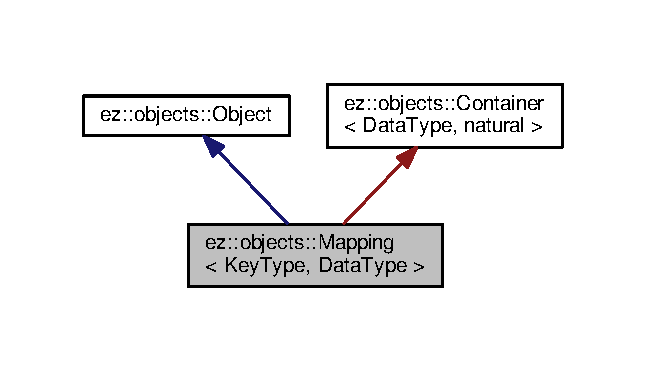
\includegraphics[width=310pt]{classez_1_1objects_1_1Mapping__inherit__graph}
\end{center}
\end{figure}


Collaboration diagram for ez\+:\+:objects\+:\+:Mapping$<$ Key\+Type, Data\+Type $>$\+:
\nopagebreak
\begin{figure}[H]
\begin{center}
\leavevmode
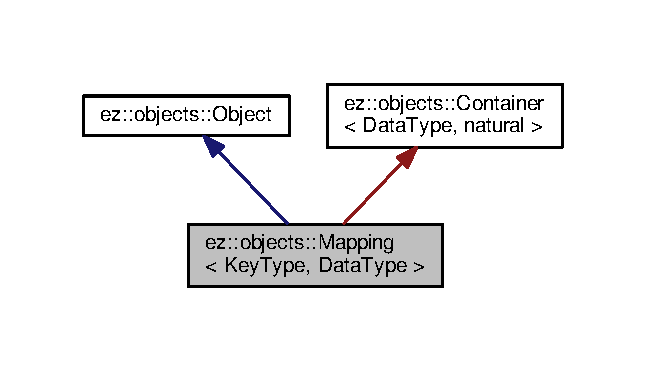
\includegraphics[width=310pt]{classez_1_1objects_1_1Mapping__coll__graph}
\end{center}
\end{figure}
\subsection*{Public Types}
\begin{DoxyCompactItemize}
\item 
\mbox{\Hypertarget{classez_1_1objects_1_1Mapping_a990b23e3d9619eaa026247d0dee44076}\label{classez_1_1objects_1_1Mapping_a990b23e3d9619eaa026247d0dee44076}} 
typedef std\+::map$<$ Key\+Type, Data\+Type $>$ {\bfseries self}
\item 
\mbox{\Hypertarget{classez_1_1objects_1_1Mapping_a1a0dde6f2975df504001a30fa4354387}\label{classez_1_1objects_1_1Mapping_a1a0dde6f2975df504001a30fa4354387}} 
typedef std\+::map$<$ Key\+Type, Data\+Type $>$\+::iterator {\bfseries iterator}
\end{DoxyCompactItemize}
\subsection*{Public Member Functions}
\begin{DoxyCompactItemize}
\item 
\hyperlink{classez_1_1objects_1_1Mapping_a12a266ba49d22f9a382a4cc916253284}{Mapping} ()
\item 
\hyperlink{classez_1_1objects_1_1Mapping_a2e01d47b23e082e6aade1923fede999d}{Mapping} (const \hyperlink{classez_1_1objects_1_1Mapping}{Mapping}$<$ Key\+Type, Data\+Type $>$ \&obj)
\item 
\hyperlink{classez_1_1objects_1_1Mapping}{Mapping}$<$ Key\+Type, Data\+Type $>$ \& \hyperlink{classez_1_1objects_1_1Mapping_a62fd1fa4b2087fc0deaafa92aaba1c0b}{operator=} (const \hyperlink{classez_1_1objects_1_1Mapping}{Mapping}$<$ Key\+Type, Data\+Type $>$ \&obj)
\item 
\hyperlink{classez_1_1objects_1_1Mapping_af2a29688f35f5a161744c111f6ec9be0}{$\sim$\+Mapping} ()
\item 
natural \hyperlink{classez_1_1objects_1_1Mapping_a223f5d523a0f3cc3eff5dc7cbf78ce29}{size} ()
\item 
\mbox{\Hypertarget{classez_1_1objects_1_1Mapping_a40d390667d1a9cce1bb00e4128800a1e}\label{classez_1_1objects_1_1Mapping_a40d390667d1a9cce1bb00e4128800a1e}} 
bool {\bfseries has\+\_\+key} (Key\+Type k)
\item 
\mbox{\Hypertarget{classez_1_1objects_1_1Mapping_addba04e486fac91d1ede7ef1af2f7c6a}\label{classez_1_1objects_1_1Mapping_addba04e486fac91d1ede7ef1af2f7c6a}} 
Data\+Type \& {\bfseries find} (Key\+Type k)
\item 
\mbox{\Hypertarget{classez_1_1objects_1_1Mapping_ae018c78b91c3b6d3189d102758d180f1}\label{classez_1_1objects_1_1Mapping_ae018c78b91c3b6d3189d102758d180f1}} 
void {\bfseries remove} (Key\+Type k)
\item 
\mbox{\Hypertarget{classez_1_1objects_1_1Mapping_a085397df2df6e39e2a144fc6e583a309}\label{classez_1_1objects_1_1Mapping_a085397df2df6e39e2a144fc6e583a309}} 
void {\bfseries put} (Key\+Type k, Data\+Type v)
\item 
void \hyperlink{classez_1_1objects_1_1Mapping_ac30b4bf58f51ea49c8422dfce1e6cf15}{print} (std\+::ostream \&stream) override
\item 
void \hyperlink{classez_1_1objects_1_1Mapping_a1233daf5c8f5d7ad9539e9d7f58703c3}{output} (std\+::ostream \&stream) override
\item 
void \hyperlink{classez_1_1objects_1_1Mapping_ad47e98279b853fd10614a24dc201d92e}{input} (std\+::istream \&stream) override
\item 
integer \hyperlink{classez_1_1objects_1_1Mapping_a7eb092099b5f47b101e5c54a46373ff0}{compare} (const \hyperlink{classez_1_1objects_1_1Object}{Object} \&y) override
\item 
\hyperlink{classez_1_1objects_1_1Object}{Object} $\ast$ \hyperlink{classez_1_1objects_1_1Mapping_aa8eb01c13630ff6ab44438e9a25aa019}{clone} () override
\item 
bool \hyperlink{classez_1_1objects_1_1Mapping_a8c7cf83ebf29a35ab146e1a1d0955907}{is\+\_\+empty} ()
\item 
void \hyperlink{classez_1_1objects_1_1Mapping_a7986873197eb0ab7199567f8c0ace175}{to\+\_\+vector} (\hyperlink{classez_1_1objects_1_1Vector}{ez\+::objects\+::\+Vector}$<$ \hyperlink{classez_1_1objects_1_1Couple}{Couple}$<$ Key\+Type, Data\+Type $>$$>$ \&v)
\item 
\mbox{\Hypertarget{classez_1_1objects_1_1Mapping_a4a59e3a56359826f390771309116d077}\label{classez_1_1objects_1_1Mapping_a4a59e3a56359826f390771309116d077}} 
iterator {\bfseries begin} ()
\item 
\mbox{\Hypertarget{classez_1_1objects_1_1Mapping_afe494ca1f8f80fbe796fa41f33608582}\label{classez_1_1objects_1_1Mapping_afe494ca1f8f80fbe796fa41f33608582}} 
iterator {\bfseries end} ()
\end{DoxyCompactItemize}
\subsection*{Protected Attributes}
\begin{DoxyCompactItemize}
\item 
\mbox{\Hypertarget{classez_1_1objects_1_1Mapping_a5a842f943216955b68dc46605d93e1d7}\label{classez_1_1objects_1_1Mapping_a5a842f943216955b68dc46605d93e1d7}} 
std\+::map$<$ Key\+Type, Data\+Type $>$ {\bfseries data}
\end{DoxyCompactItemize}
\subsection*{Additional Inherited Members}


\subsection{Constructor \& Destructor Documentation}
\mbox{\Hypertarget{classez_1_1objects_1_1Mapping_a12a266ba49d22f9a382a4cc916253284}\label{classez_1_1objects_1_1Mapping_a12a266ba49d22f9a382a4cc916253284}} 
\index{ez\+::objects\+::\+Mapping@{ez\+::objects\+::\+Mapping}!Mapping@{Mapping}}
\index{Mapping@{Mapping}!ez\+::objects\+::\+Mapping@{ez\+::objects\+::\+Mapping}}
\subsubsection{\texorpdfstring{Mapping()}{Mapping()}\hspace{0.1cm}{\footnotesize\ttfamily [1/2]}}
{\footnotesize\ttfamily template$<$class Key\+Type, class Data\+Type$>$ \\
\hyperlink{classez_1_1objects_1_1Mapping}{ez\+::objects\+::\+Mapping}$<$ Key\+Type, Data\+Type $>$\+::\hyperlink{classez_1_1objects_1_1Mapping}{Mapping} (\begin{DoxyParamCaption}{ }\end{DoxyParamCaption})\hspace{0.3cm}{\ttfamily [inline]}}

Default constructor \mbox{\Hypertarget{classez_1_1objects_1_1Mapping_a2e01d47b23e082e6aade1923fede999d}\label{classez_1_1objects_1_1Mapping_a2e01d47b23e082e6aade1923fede999d}} 
\index{ez\+::objects\+::\+Mapping@{ez\+::objects\+::\+Mapping}!Mapping@{Mapping}}
\index{Mapping@{Mapping}!ez\+::objects\+::\+Mapping@{ez\+::objects\+::\+Mapping}}
\subsubsection{\texorpdfstring{Mapping()}{Mapping()}\hspace{0.1cm}{\footnotesize\ttfamily [2/2]}}
{\footnotesize\ttfamily template$<$class Key\+Type, class Data\+Type$>$ \\
\hyperlink{classez_1_1objects_1_1Mapping}{ez\+::objects\+::\+Mapping}$<$ Key\+Type, Data\+Type $>$\+::\hyperlink{classez_1_1objects_1_1Mapping}{Mapping} (\begin{DoxyParamCaption}\item[{const \hyperlink{classez_1_1objects_1_1Mapping}{Mapping}$<$ Key\+Type, Data\+Type $>$ \&}]{obj }\end{DoxyParamCaption})\hspace{0.3cm}{\ttfamily [inline]}}

Copy constructor \mbox{\Hypertarget{classez_1_1objects_1_1Mapping_af2a29688f35f5a161744c111f6ec9be0}\label{classez_1_1objects_1_1Mapping_af2a29688f35f5a161744c111f6ec9be0}} 
\index{ez\+::objects\+::\+Mapping@{ez\+::objects\+::\+Mapping}!````~Mapping@{$\sim$\+Mapping}}
\index{````~Mapping@{$\sim$\+Mapping}!ez\+::objects\+::\+Mapping@{ez\+::objects\+::\+Mapping}}
\subsubsection{\texorpdfstring{$\sim$\+Mapping()}{~Mapping()}}
{\footnotesize\ttfamily template$<$class Key\+Type, class Data\+Type$>$ \\
\hyperlink{classez_1_1objects_1_1Mapping}{ez\+::objects\+::\+Mapping}$<$ Key\+Type, Data\+Type $>$\+::$\sim$\hyperlink{classez_1_1objects_1_1Mapping}{Mapping} (\begin{DoxyParamCaption}{ }\end{DoxyParamCaption})\hspace{0.3cm}{\ttfamily [inline]}}

Destructor 

\subsection{Member Function Documentation}
\mbox{\Hypertarget{classez_1_1objects_1_1Mapping_aa8eb01c13630ff6ab44438e9a25aa019}\label{classez_1_1objects_1_1Mapping_aa8eb01c13630ff6ab44438e9a25aa019}} 
\index{ez\+::objects\+::\+Mapping@{ez\+::objects\+::\+Mapping}!clone@{clone}}
\index{clone@{clone}!ez\+::objects\+::\+Mapping@{ez\+::objects\+::\+Mapping}}
\subsubsection{\texorpdfstring{clone()}{clone()}}
{\footnotesize\ttfamily template$<$class Key\+Type, class Data\+Type$>$ \\
\hyperlink{classez_1_1objects_1_1Object}{Object}$\ast$ \hyperlink{classez_1_1objects_1_1Mapping}{ez\+::objects\+::\+Mapping}$<$ Key\+Type, Data\+Type $>$\+::clone (\begin{DoxyParamCaption}{ }\end{DoxyParamCaption})\hspace{0.3cm}{\ttfamily [inline]}, {\ttfamily [override]}, {\ttfamily [virtual]}}

return a copy of the object 

Reimplemented from \hyperlink{classez_1_1objects_1_1Object_acf444b2581d898eb4b8c92c2d5865c9e}{ez\+::objects\+::\+Object}.

\mbox{\Hypertarget{classez_1_1objects_1_1Mapping_a7eb092099b5f47b101e5c54a46373ff0}\label{classez_1_1objects_1_1Mapping_a7eb092099b5f47b101e5c54a46373ff0}} 
\index{ez\+::objects\+::\+Mapping@{ez\+::objects\+::\+Mapping}!compare@{compare}}
\index{compare@{compare}!ez\+::objects\+::\+Mapping@{ez\+::objects\+::\+Mapping}}
\subsubsection{\texorpdfstring{compare()}{compare()}}
{\footnotesize\ttfamily template$<$class Key\+Type, class Data\+Type$>$ \\
integer \hyperlink{classez_1_1objects_1_1Mapping}{ez\+::objects\+::\+Mapping}$<$ Key\+Type, Data\+Type $>$\+::compare (\begin{DoxyParamCaption}\item[{const \hyperlink{classez_1_1objects_1_1Object}{Object} \&}]{y }\end{DoxyParamCaption})\hspace{0.3cm}{\ttfamily [inline]}, {\ttfamily [override]}, {\ttfamily [virtual]}}

compare two objects \begin{DoxyReturn}{Returns}
0 if objects are identical, negative value if this $<$ y, positive value if this $>$ y 
\end{DoxyReturn}


Reimplemented from \hyperlink{classez_1_1objects_1_1Object_aca311d389dffa204e425463145f4e1e6}{ez\+::objects\+::\+Object}.

\mbox{\Hypertarget{classez_1_1objects_1_1Mapping_ad47e98279b853fd10614a24dc201d92e}\label{classez_1_1objects_1_1Mapping_ad47e98279b853fd10614a24dc201d92e}} 
\index{ez\+::objects\+::\+Mapping@{ez\+::objects\+::\+Mapping}!input@{input}}
\index{input@{input}!ez\+::objects\+::\+Mapping@{ez\+::objects\+::\+Mapping}}
\subsubsection{\texorpdfstring{input()}{input()}}
{\footnotesize\ttfamily template$<$class Key\+Type, class Data\+Type$>$ \\
void \hyperlink{classez_1_1objects_1_1Mapping}{ez\+::objects\+::\+Mapping}$<$ Key\+Type, Data\+Type $>$\+::input (\begin{DoxyParamCaption}\item[{std\+::istream \&}]{stream }\end{DoxyParamCaption})\hspace{0.3cm}{\ttfamily [inline]}, {\ttfamily [override]}, {\ttfamily [virtual]}}

this function is used to get the data field members of an object from a stream and acts as unserialize 

Reimplemented from \hyperlink{classez_1_1objects_1_1Object_a878bdc53b7f16fda6fa15dab214c4b6a}{ez\+::objects\+::\+Object}.

\mbox{\Hypertarget{classez_1_1objects_1_1Mapping_a8c7cf83ebf29a35ab146e1a1d0955907}\label{classez_1_1objects_1_1Mapping_a8c7cf83ebf29a35ab146e1a1d0955907}} 
\index{ez\+::objects\+::\+Mapping@{ez\+::objects\+::\+Mapping}!is\+\_\+empty@{is\+\_\+empty}}
\index{is\+\_\+empty@{is\+\_\+empty}!ez\+::objects\+::\+Mapping@{ez\+::objects\+::\+Mapping}}
\subsubsection{\texorpdfstring{is\+\_\+empty()}{is\_empty()}}
{\footnotesize\ttfamily template$<$class Key\+Type, class Data\+Type$>$ \\
bool \hyperlink{classez_1_1objects_1_1Mapping}{ez\+::objects\+::\+Mapping}$<$ Key\+Type, Data\+Type $>$\+::is\+\_\+empty (\begin{DoxyParamCaption}{ }\end{DoxyParamCaption})\hspace{0.3cm}{\ttfamily [inline]}, {\ttfamily [virtual]}}

Return true if container has no element, false otherwise 

Implements \hyperlink{classez_1_1objects_1_1Container_a205eb4f8a4fe967d425fdf04e5db5f93}{ez\+::objects\+::\+Container$<$ Data\+Type, natural $>$}.

\mbox{\Hypertarget{classez_1_1objects_1_1Mapping_a62fd1fa4b2087fc0deaafa92aaba1c0b}\label{classez_1_1objects_1_1Mapping_a62fd1fa4b2087fc0deaafa92aaba1c0b}} 
\index{ez\+::objects\+::\+Mapping@{ez\+::objects\+::\+Mapping}!operator=@{operator=}}
\index{operator=@{operator=}!ez\+::objects\+::\+Mapping@{ez\+::objects\+::\+Mapping}}
\subsubsection{\texorpdfstring{operator=()}{operator=()}}
{\footnotesize\ttfamily template$<$class Key\+Type, class Data\+Type$>$ \\
\hyperlink{classez_1_1objects_1_1Mapping}{Mapping}$<$Key\+Type, Data\+Type$>$\& \hyperlink{classez_1_1objects_1_1Mapping}{ez\+::objects\+::\+Mapping}$<$ Key\+Type, Data\+Type $>$\+::operator= (\begin{DoxyParamCaption}\item[{const \hyperlink{classez_1_1objects_1_1Mapping}{Mapping}$<$ Key\+Type, Data\+Type $>$ \&}]{obj }\end{DoxyParamCaption})\hspace{0.3cm}{\ttfamily [inline]}}

Assignment operator \mbox{\Hypertarget{classez_1_1objects_1_1Mapping_a1233daf5c8f5d7ad9539e9d7f58703c3}\label{classez_1_1objects_1_1Mapping_a1233daf5c8f5d7ad9539e9d7f58703c3}} 
\index{ez\+::objects\+::\+Mapping@{ez\+::objects\+::\+Mapping}!output@{output}}
\index{output@{output}!ez\+::objects\+::\+Mapping@{ez\+::objects\+::\+Mapping}}
\subsubsection{\texorpdfstring{output()}{output()}}
{\footnotesize\ttfamily template$<$class Key\+Type, class Data\+Type$>$ \\
void \hyperlink{classez_1_1objects_1_1Mapping}{ez\+::objects\+::\+Mapping}$<$ Key\+Type, Data\+Type $>$\+::output (\begin{DoxyParamCaption}\item[{std\+::ostream \&}]{stream }\end{DoxyParamCaption})\hspace{0.3cm}{\ttfamily [inline]}, {\ttfamily [override]}, {\ttfamily [virtual]}}

this function is used to print the contents of the object in a serializable manner 

Reimplemented from \hyperlink{classez_1_1objects_1_1Object_a0fdfe18e6c35d6b0d7e7a01265aded15}{ez\+::objects\+::\+Object}.

\mbox{\Hypertarget{classez_1_1objects_1_1Mapping_ac30b4bf58f51ea49c8422dfce1e6cf15}\label{classez_1_1objects_1_1Mapping_ac30b4bf58f51ea49c8422dfce1e6cf15}} 
\index{ez\+::objects\+::\+Mapping@{ez\+::objects\+::\+Mapping}!print@{print}}
\index{print@{print}!ez\+::objects\+::\+Mapping@{ez\+::objects\+::\+Mapping}}
\subsubsection{\texorpdfstring{print()}{print()}}
{\footnotesize\ttfamily template$<$class Key\+Type, class Data\+Type$>$ \\
void \hyperlink{classez_1_1objects_1_1Mapping}{ez\+::objects\+::\+Mapping}$<$ Key\+Type, Data\+Type $>$\+::print (\begin{DoxyParamCaption}\item[{std\+::ostream \&}]{stream }\end{DoxyParamCaption})\hspace{0.3cm}{\ttfamily [inline]}, {\ttfamily [override]}, {\ttfamily [virtual]}}

overloading of print method of class \hyperlink{classez_1_1objects_1_1Object}{Object} 

Reimplemented from \hyperlink{classez_1_1objects_1_1Object_a9e20f39a78163f67f000576149d858b3}{ez\+::objects\+::\+Object}.

\mbox{\Hypertarget{classez_1_1objects_1_1Mapping_a223f5d523a0f3cc3eff5dc7cbf78ce29}\label{classez_1_1objects_1_1Mapping_a223f5d523a0f3cc3eff5dc7cbf78ce29}} 
\index{ez\+::objects\+::\+Mapping@{ez\+::objects\+::\+Mapping}!size@{size}}
\index{size@{size}!ez\+::objects\+::\+Mapping@{ez\+::objects\+::\+Mapping}}
\subsubsection{\texorpdfstring{size()}{size()}}
{\footnotesize\ttfamily template$<$class Key\+Type, class Data\+Type$>$ \\
natural \hyperlink{classez_1_1objects_1_1Mapping}{ez\+::objects\+::\+Mapping}$<$ Key\+Type, Data\+Type $>$\+::size (\begin{DoxyParamCaption}{ }\end{DoxyParamCaption})\hspace{0.3cm}{\ttfamily [inline]}, {\ttfamily [virtual]}}

Return number of elements 

Implements \hyperlink{classez_1_1objects_1_1Container_affd294810c6c29530d1d1e3c2151ad28}{ez\+::objects\+::\+Container$<$ Data\+Type, natural $>$}.

\mbox{\Hypertarget{classez_1_1objects_1_1Mapping_a7986873197eb0ab7199567f8c0ace175}\label{classez_1_1objects_1_1Mapping_a7986873197eb0ab7199567f8c0ace175}} 
\index{ez\+::objects\+::\+Mapping@{ez\+::objects\+::\+Mapping}!to\+\_\+vector@{to\+\_\+vector}}
\index{to\+\_\+vector@{to\+\_\+vector}!ez\+::objects\+::\+Mapping@{ez\+::objects\+::\+Mapping}}
\subsubsection{\texorpdfstring{to\+\_\+vector()}{to\_vector()}}
{\footnotesize\ttfamily template$<$class Key\+Type, class Data\+Type$>$ \\
void \hyperlink{classez_1_1objects_1_1Mapping}{ez\+::objects\+::\+Mapping}$<$ Key\+Type, Data\+Type $>$\+::to\+\_\+vector (\begin{DoxyParamCaption}\item[{\hyperlink{classez_1_1objects_1_1Vector}{ez\+::objects\+::\+Vector}$<$ \hyperlink{classez_1_1objects_1_1Couple}{Couple}$<$ Key\+Type, Data\+Type $>$$>$ \&}]{v }\end{DoxyParamCaption})\hspace{0.3cm}{\ttfamily [inline]}}

convert mapping to vector of pairs in order to apply sort for example 

The documentation for this class was generated from the following file\+:\begin{DoxyCompactItemize}
\item 
src/version\+\_\+2018.\+06/objects/mapping.\+h\end{DoxyCompactItemize}

\hypertarget{classez_1_1maths_1_1Matrix}{}\section{ez\+:\+:maths\+:\+:Matrix$<$ Data\+Type $>$ Class Template Reference}
\label{classez_1_1maths_1_1Matrix}\index{ez\+::maths\+::\+Matrix$<$ Data\+Type $>$@{ez\+::maths\+::\+Matrix$<$ Data\+Type $>$}}


{\ttfamily \#include $<$matrix.\+h$>$}

\subsection*{Data Structures}
\begin{DoxyCompactItemize}
\item 
class \hyperlink{classez_1_1maths_1_1Matrix_1_1MatrixRow}{Matrix\+Row}
\end{DoxyCompactItemize}
\subsection*{Public Types}
\begin{DoxyCompactItemize}
\item 
\mbox{\Hypertarget{classez_1_1maths_1_1Matrix_afe4c29ded12f4b2c40795da3d6580c46}\label{classez_1_1maths_1_1Matrix_afe4c29ded12f4b2c40795da3d6580c46}} 
typedef \hyperlink{classez_1_1maths_1_1Matrix}{Matrix}$<$ Data\+Type $>$ {\bfseries self}
\item 
\mbox{\Hypertarget{classez_1_1maths_1_1Matrix_aa699b296a08c9251239f307cd42f4b3d}\label{classez_1_1maths_1_1Matrix_aa699b296a08c9251239f307cd42f4b3d}} 
typedef Data\+Type {\bfseries value\+\_\+type}
\item 
\mbox{\Hypertarget{classez_1_1maths_1_1Matrix_ae6a09a08df99df89846f5026087f3d2b}\label{classez_1_1maths_1_1Matrix_ae6a09a08df99df89846f5026087f3d2b}} 
typedef std\+::vector$<$ Data\+Type $>$\+::iterator {\bfseries iterator}
\end{DoxyCompactItemize}
\subsection*{Public Member Functions}
\begin{DoxyCompactItemize}
\item 
\hyperlink{classez_1_1maths_1_1Matrix_ab1ee41b4f342b94006853dc7213ab179}{Matrix} ()
\item 
\hyperlink{classez_1_1maths_1_1Matrix_a97b95c8be7fd18cf0beb2789dee19b2a}{Matrix} (natural rows, natural cols)
\item 
\mbox{\Hypertarget{classez_1_1maths_1_1Matrix_a165b105b7f0457c5fe85448c44b08abe}\label{classez_1_1maths_1_1Matrix_a165b105b7f0457c5fe85448c44b08abe}} 
{\bfseries Matrix} (const \hyperlink{classez_1_1maths_1_1Matrix}{Matrix}$<$ Data\+Type $>$ \&obj)
\item 
\mbox{\Hypertarget{classez_1_1maths_1_1Matrix_ad4600cc7e192a7c76858e3a629e71c91}\label{classez_1_1maths_1_1Matrix_ad4600cc7e192a7c76858e3a629e71c91}} 
{\bfseries Matrix} (natural size\+\_\+y, natural size\+\_\+x, const std\+::initializer\+\_\+list$<$ Data\+Type $>$ \&l)
\item 
\mbox{\Hypertarget{classez_1_1maths_1_1Matrix_ada5bd4986817d885f9bd33c7726618e9}\label{classez_1_1maths_1_1Matrix_ada5bd4986817d885f9bd33c7726618e9}} 
\hyperlink{classez_1_1maths_1_1Matrix}{Matrix}$<$ Data\+Type $>$ \& {\bfseries operator=} (const \hyperlink{classez_1_1maths_1_1Matrix}{Matrix}$<$ Data\+Type $>$ \&obj)
\item 
\mbox{\Hypertarget{classez_1_1maths_1_1Matrix_a08f19b4b97c7e970b656d4f7ed520a3d}\label{classez_1_1maths_1_1Matrix_a08f19b4b97c7e970b656d4f7ed520a3d}} 
natural {\bfseries size} ()
\item 
\mbox{\Hypertarget{classez_1_1maths_1_1Matrix_a1c74dfc803ad0827c02fda54a811e518}\label{classez_1_1maths_1_1Matrix_a1c74dfc803ad0827c02fda54a811e518}} 
natural {\bfseries size\+\_\+x} ()
\item 
\mbox{\Hypertarget{classez_1_1maths_1_1Matrix_a5648d269f07126af169f6667915ffc93}\label{classez_1_1maths_1_1Matrix_a5648d269f07126af169f6667915ffc93}} 
natural {\bfseries size\+\_\+y} ()
\item 
\mbox{\Hypertarget{classez_1_1maths_1_1Matrix_ab99b87184b37758d922b18bc930b07bd}\label{classez_1_1maths_1_1Matrix_ab99b87184b37758d922b18bc930b07bd}} 
natural {\bfseries dim} (natural d=0)
\item 
\mbox{\Hypertarget{classez_1_1maths_1_1Matrix_a7b1faaa410f83a2e1c9ae296e4dc7fe6}\label{classez_1_1maths_1_1Matrix_a7b1faaa410f83a2e1c9ae296e4dc7fe6}} 
std\+::vector$<$ Data\+Type $>$ \& {\bfseries data} ()
\item 
\mbox{\Hypertarget{classez_1_1maths_1_1Matrix_a7e22335d5a6bbd952e3c2ab2cb862a29}\label{classez_1_1maths_1_1Matrix_a7e22335d5a6bbd952e3c2ab2cb862a29}} 
void {\bfseries resize} (natural size\+\_\+y, natural size\+\_\+x)
\item 
void \hyperlink{classez_1_1maths_1_1Matrix_ac2a273c2fae9801582a23e119cd89676}{fill} (Data\+Type value)
\item 
\mbox{\Hypertarget{classez_1_1maths_1_1Matrix_a92f12ab6e400f003b1fd6a115a84f5bb}\label{classez_1_1maths_1_1Matrix_a92f12ab6e400f003b1fd6a115a84f5bb}} 
void {\bfseries fill\+\_\+row} (natural y, Data\+Type value)
\item 
Data\+Type \hyperlink{classez_1_1maths_1_1Matrix_aa0476234c21980c3896cd0c535aa935c}{dot} (natural index=1, natural axis=0)
\item 
\mbox{\Hypertarget{classez_1_1maths_1_1Matrix_a40635b102148f88d5c372e5df07c463e}\label{classez_1_1maths_1_1Matrix_a40635b102148f88d5c372e5df07c463e}} 
\hyperlink{classez_1_1maths_1_1Matrix_1_1MatrixRow}{Matrix\+Row} {\bfseries operator\mbox{[}$\,$\mbox{]}} (natural y)
\item 
Data\+Type \& \hyperlink{classez_1_1maths_1_1Matrix_a9fdf7683e9eec9f72feedf202c98f5aa}{operator()} (natural y, natural x)
\item 
\mbox{\Hypertarget{classez_1_1maths_1_1Matrix_a016c8c4cfab8f4544020fcfa52b3e5d7}\label{classez_1_1maths_1_1Matrix_a016c8c4cfab8f4544020fcfa52b3e5d7}} 
\hyperlink{classez_1_1maths_1_1Matrix}{self} {\bfseries operator+} (const \hyperlink{classez_1_1maths_1_1Matrix}{self} \&b)
\item 
\mbox{\Hypertarget{classez_1_1maths_1_1Matrix_a603b18b52b3e0c01ac13eaeed176b1c3}\label{classez_1_1maths_1_1Matrix_a603b18b52b3e0c01ac13eaeed176b1c3}} 
\hyperlink{classez_1_1maths_1_1Matrix}{self} \& {\bfseries operator+=} (const \hyperlink{classez_1_1maths_1_1Matrix}{self} \&b)
\item 
\mbox{\Hypertarget{classez_1_1maths_1_1Matrix_a5a8b2436a5300bd008afedb7bd24891b}\label{classez_1_1maths_1_1Matrix_a5a8b2436a5300bd008afedb7bd24891b}} 
\hyperlink{classez_1_1maths_1_1Matrix}{self} \& {\bfseries operator-\/=} (const \hyperlink{classez_1_1maths_1_1Matrix}{self} \&b)
\item 
\mbox{\Hypertarget{classez_1_1maths_1_1Matrix_ac2ecb9219b7c3c822a8af597e47f0283}\label{classez_1_1maths_1_1Matrix_ac2ecb9219b7c3c822a8af597e47f0283}} 
\hyperlink{classez_1_1maths_1_1Matrix}{self} {\bfseries operator$\ast$} (const \hyperlink{classez_1_1maths_1_1Matrix}{self} \&b)
\item 
\mbox{\Hypertarget{classez_1_1maths_1_1Matrix_ac17580a4d464b3c849cf52b74cd6607d}\label{classez_1_1maths_1_1Matrix_ac17580a4d464b3c849cf52b74cd6607d}} 
\hyperlink{classez_1_1maths_1_1Matrix}{self} \& {\bfseries operator$\ast$=} (const \hyperlink{classez_1_1maths_1_1Matrix}{self} \&b)
\item 
\mbox{\Hypertarget{classez_1_1maths_1_1Matrix_add06a09122f9d982655fa0b6a2c723fc}\label{classez_1_1maths_1_1Matrix_add06a09122f9d982655fa0b6a2c723fc}} 
integer {\bfseries compare} (const \hyperlink{classez_1_1maths_1_1Matrix}{self} \&y)
\item 
\mbox{\Hypertarget{classez_1_1maths_1_1Matrix_a3b7e8b5d99b96d5bbea681ea2e806cd9}\label{classez_1_1maths_1_1Matrix_a3b7e8b5d99b96d5bbea681ea2e806cd9}} 
iterator {\bfseries begin} ()
\item 
\mbox{\Hypertarget{classez_1_1maths_1_1Matrix_aa9935d5a54edca1edaa39c8267cb9d78}\label{classez_1_1maths_1_1Matrix_aa9935d5a54edca1edaa39c8267cb9d78}} 
iterator {\bfseries end} ()
\item 
void \hyperlink{classez_1_1maths_1_1Matrix_a28472a82209513ed5934209c0e8b5a7a}{prod} (\hyperlink{classez_1_1maths_1_1Vector}{ez\+::maths\+::\+Vector}$<$ Data\+Type $>$ \&result, \hyperlink{classez_1_1maths_1_1Vector}{ez\+::maths\+::\+Vector}$<$ Data\+Type $>$ \&v)
\item 
\mbox{\Hypertarget{classez_1_1maths_1_1Matrix_a7a0682d82824b3d994786cbccbec2a03}\label{classez_1_1maths_1_1Matrix_a7a0682d82824b3d994786cbccbec2a03}} 
void {\bfseries transpose} ()
\item 
\mbox{\Hypertarget{classez_1_1maths_1_1Matrix_a5f08d49f2e49d4bc32dc2452933f1093}\label{classez_1_1maths_1_1Matrix_a5f08d49f2e49d4bc32dc2452933f1093}} 
void {\bfseries remove\+\_\+row} (natural n)
\item 
\mbox{\Hypertarget{classez_1_1maths_1_1Matrix_a1007c648a87f5e9dab3d9225be604e45}\label{classez_1_1maths_1_1Matrix_a1007c648a87f5e9dab3d9225be604e45}} 
void {\bfseries remove\+\_\+column} (natural n)
\item 
\mbox{\Hypertarget{classez_1_1maths_1_1Matrix_aed27f1b29878684ee27af417122a0084}\label{classez_1_1maths_1_1Matrix_aed27f1b29878684ee27af417122a0084}} 
Data\+Type {\bfseries sum} (Data\+Type init=0)
\item 
\mbox{\Hypertarget{classez_1_1maths_1_1Matrix_aa5ef70156e11adf93b188af921366332}\label{classez_1_1maths_1_1Matrix_aa5ef70156e11adf93b188af921366332}} 
void {\bfseries vec\+\_\+mul\+\_\+sum} (\hyperlink{classez_1_1maths_1_1Matrix}{self} \&v, \hyperlink{classez_1_1maths_1_1Matrix}{self} \&r)
\item 
\mbox{\Hypertarget{classez_1_1maths_1_1Matrix_a3ebde4c806e787916b78fee9b73d89ed}\label{classez_1_1maths_1_1Matrix_a3ebde4c806e787916b78fee9b73d89ed}} 
Data\+Type {\bfseries mat\+\_\+mul\+\_\+sum} (\hyperlink{classez_1_1maths_1_1Matrix}{self} \&m)
\end{DoxyCompactItemize}
\subsection*{Data Fields}
\begin{DoxyCompactItemize}
\item 
std\+::vector$<$ Data\+Type $>$ \hyperlink{classez_1_1maths_1_1Matrix_a185697a4eb9527a6c3f0ecf59975f181}{m\+\_\+data}
\item 
natural \hyperlink{classez_1_1maths_1_1Matrix_a57afd79b657d3ca032728559e0674000}{m\+\_\+size\+\_\+x}
\item 
\mbox{\Hypertarget{classez_1_1maths_1_1Matrix_a8ec6800329545f6c5c2658c44b0c718b}\label{classez_1_1maths_1_1Matrix_a8ec6800329545f6c5c2658c44b0c718b}} 
natural {\bfseries m\+\_\+size\+\_\+y}
\end{DoxyCompactItemize}
\subsection*{Friends}
\begin{DoxyCompactItemize}
\item 
\mbox{\Hypertarget{classez_1_1maths_1_1Matrix_a0f01ab4d11317fc6cdd4af4f049e2727}\label{classez_1_1maths_1_1Matrix_a0f01ab4d11317fc6cdd4af4f049e2727}} 
std\+::ostream \& {\bfseries operator$<$$<$} (std\+::ostream \&out, \hyperlink{classez_1_1maths_1_1Matrix}{Matrix}$<$ Data\+Type $>$ \&m)
\item 
\mbox{\Hypertarget{classez_1_1maths_1_1Matrix_a89b571e0607100045577d5023a77342b}\label{classez_1_1maths_1_1Matrix_a89b571e0607100045577d5023a77342b}} 
bool {\bfseries operator==} (const \hyperlink{classez_1_1maths_1_1Matrix}{self} \&x, const \hyperlink{classez_1_1maths_1_1Matrix}{self} \&y)
\item 
\mbox{\Hypertarget{classez_1_1maths_1_1Matrix_a7b7b1149640de716ebef2e91527b695f}\label{classez_1_1maths_1_1Matrix_a7b7b1149640de716ebef2e91527b695f}} 
\hyperlink{classez_1_1maths_1_1Vector}{Vector}$<$ Data\+Type $>$ {\bfseries operator$\ast$} (\hyperlink{classez_1_1maths_1_1Matrix}{Matrix}$<$ Data\+Type $>$ \&m, \hyperlink{classez_1_1maths_1_1Vector}{Vector}$<$ Data\+Type $>$ \&v)
\item 
\mbox{\Hypertarget{classez_1_1maths_1_1Matrix_ada11ca1e5476b320d044ea2b94431ded}\label{classez_1_1maths_1_1Matrix_ada11ca1e5476b320d044ea2b94431ded}} 
\hyperlink{classez_1_1maths_1_1Vector}{Vector}$<$ Data\+Type $>$ {\bfseries operator$\ast$} (\hyperlink{classez_1_1maths_1_1Vector}{Vector}$<$ Data\+Type $>$ \&v, \hyperlink{classez_1_1maths_1_1Matrix}{Matrix}$<$ Data\+Type $>$ \&m)
\item 
\mbox{\Hypertarget{classez_1_1maths_1_1Matrix_a4eda110f2ff2f92546170cbc4a198e05}\label{classez_1_1maths_1_1Matrix_a4eda110f2ff2f92546170cbc4a198e05}} 
bool {\bfseries operator$<$} (const \hyperlink{classez_1_1maths_1_1Matrix}{self} \&x, const \hyperlink{classez_1_1maths_1_1Matrix}{self} \&y)
\item 
\mbox{\Hypertarget{classez_1_1maths_1_1Matrix_a9e89bf77c37246bc1e7c1b9f59a5e369}\label{classez_1_1maths_1_1Matrix_a9e89bf77c37246bc1e7c1b9f59a5e369}} 
bool {\bfseries operator$<$=} (const \hyperlink{classez_1_1maths_1_1Matrix}{self} \&x, const \hyperlink{classez_1_1maths_1_1Matrix}{self} \&y)
\item 
\mbox{\Hypertarget{classez_1_1maths_1_1Matrix_ae1705ad5d782614d851e1553f15f017b}\label{classez_1_1maths_1_1Matrix_ae1705ad5d782614d851e1553f15f017b}} 
bool {\bfseries operator$>$} (const \hyperlink{classez_1_1maths_1_1Matrix}{self} \&x, const \hyperlink{classez_1_1maths_1_1Matrix}{self} \&y)
\item 
\mbox{\Hypertarget{classez_1_1maths_1_1Matrix_a79ad47b0999178d78909e91cd6a50109}\label{classez_1_1maths_1_1Matrix_a79ad47b0999178d78909e91cd6a50109}} 
bool {\bfseries operator$>$=} (const \hyperlink{classez_1_1maths_1_1Matrix}{self} \&x, const \hyperlink{classez_1_1maths_1_1Matrix}{self} \&y)
\end{DoxyCompactItemize}


\subsection{Detailed Description}
\subsubsection*{template$<$class Data\+Type$>$\newline
class ez\+::maths\+::\+Matrix$<$ Data\+Type $>$}

Class that implements a matrix of scalar types 

\subsection{Constructor \& Destructor Documentation}
\mbox{\Hypertarget{classez_1_1maths_1_1Matrix_ab1ee41b4f342b94006853dc7213ab179}\label{classez_1_1maths_1_1Matrix_ab1ee41b4f342b94006853dc7213ab179}} 
\index{ez\+::maths\+::\+Matrix@{ez\+::maths\+::\+Matrix}!Matrix@{Matrix}}
\index{Matrix@{Matrix}!ez\+::maths\+::\+Matrix@{ez\+::maths\+::\+Matrix}}
\subsubsection{\texorpdfstring{Matrix()}{Matrix()}\hspace{0.1cm}{\footnotesize\ttfamily [1/2]}}
{\footnotesize\ttfamily template$<$class Data\+Type$>$ \\
\hyperlink{classez_1_1maths_1_1Matrix}{ez\+::maths\+::\+Matrix}$<$ Data\+Type $>$\+::\hyperlink{classez_1_1maths_1_1Matrix}{Matrix} (\begin{DoxyParamCaption}{ }\end{DoxyParamCaption})\hspace{0.3cm}{\ttfamily [inline]}}

default constructor \mbox{\Hypertarget{classez_1_1maths_1_1Matrix_a97b95c8be7fd18cf0beb2789dee19b2a}\label{classez_1_1maths_1_1Matrix_a97b95c8be7fd18cf0beb2789dee19b2a}} 
\index{ez\+::maths\+::\+Matrix@{ez\+::maths\+::\+Matrix}!Matrix@{Matrix}}
\index{Matrix@{Matrix}!ez\+::maths\+::\+Matrix@{ez\+::maths\+::\+Matrix}}
\subsubsection{\texorpdfstring{Matrix()}{Matrix()}\hspace{0.1cm}{\footnotesize\ttfamily [2/2]}}
{\footnotesize\ttfamily template$<$class Data\+Type$>$ \\
\hyperlink{classez_1_1maths_1_1Matrix}{ez\+::maths\+::\+Matrix}$<$ Data\+Type $>$\+::\hyperlink{classez_1_1maths_1_1Matrix}{Matrix} (\begin{DoxyParamCaption}\item[{natural}]{rows,  }\item[{natural}]{cols }\end{DoxyParamCaption})\hspace{0.3cm}{\ttfamily [inline]}}

constructor given number of rows and columns 

\subsection{Member Function Documentation}
\mbox{\Hypertarget{classez_1_1maths_1_1Matrix_aa0476234c21980c3896cd0c535aa935c}\label{classez_1_1maths_1_1Matrix_aa0476234c21980c3896cd0c535aa935c}} 
\index{ez\+::maths\+::\+Matrix@{ez\+::maths\+::\+Matrix}!dot@{dot}}
\index{dot@{dot}!ez\+::maths\+::\+Matrix@{ez\+::maths\+::\+Matrix}}
\subsubsection{\texorpdfstring{dot()}{dot()}}
{\footnotesize\ttfamily template$<$class Data\+Type$>$ \\
Data\+Type \hyperlink{classez_1_1maths_1_1Matrix}{ez\+::maths\+::\+Matrix}$<$ Data\+Type $>$\+::dot (\begin{DoxyParamCaption}\item[{natural}]{index = {\ttfamily 1},  }\item[{natural}]{axis = {\ttfamily 0} }\end{DoxyParamCaption})\hspace{0.3cm}{\ttfamily [inline]}}

return dot product of a row (axis == 0) or column (axis == 1) we can select the row or column using the index variable \mbox{\Hypertarget{classez_1_1maths_1_1Matrix_ac2a273c2fae9801582a23e119cd89676}\label{classez_1_1maths_1_1Matrix_ac2a273c2fae9801582a23e119cd89676}} 
\index{ez\+::maths\+::\+Matrix@{ez\+::maths\+::\+Matrix}!fill@{fill}}
\index{fill@{fill}!ez\+::maths\+::\+Matrix@{ez\+::maths\+::\+Matrix}}
\subsubsection{\texorpdfstring{fill()}{fill()}}
{\footnotesize\ttfamily template$<$class Data\+Type$>$ \\
void \hyperlink{classez_1_1maths_1_1Matrix}{ez\+::maths\+::\+Matrix}$<$ Data\+Type $>$\+::fill (\begin{DoxyParamCaption}\item[{Data\+Type}]{value }\end{DoxyParamCaption})\hspace{0.3cm}{\ttfamily [inline]}}

fill entire matrix with given value \mbox{\Hypertarget{classez_1_1maths_1_1Matrix_a9fdf7683e9eec9f72feedf202c98f5aa}\label{classez_1_1maths_1_1Matrix_a9fdf7683e9eec9f72feedf202c98f5aa}} 
\index{ez\+::maths\+::\+Matrix@{ez\+::maths\+::\+Matrix}!operator()@{operator()}}
\index{operator()@{operator()}!ez\+::maths\+::\+Matrix@{ez\+::maths\+::\+Matrix}}
\subsubsection{\texorpdfstring{operator()()}{operator()()}}
{\footnotesize\ttfamily template$<$class Data\+Type$>$ \\
Data\+Type\& \hyperlink{classez_1_1maths_1_1Matrix}{ez\+::maths\+::\+Matrix}$<$ Data\+Type $>$\+::operator() (\begin{DoxyParamCaption}\item[{natural}]{y,  }\item[{natural}]{x }\end{DoxyParamCaption})\hspace{0.3cm}{\ttfamily [inline]}}

return reference to element (y,x) \mbox{\Hypertarget{classez_1_1maths_1_1Matrix_a28472a82209513ed5934209c0e8b5a7a}\label{classez_1_1maths_1_1Matrix_a28472a82209513ed5934209c0e8b5a7a}} 
\index{ez\+::maths\+::\+Matrix@{ez\+::maths\+::\+Matrix}!prod@{prod}}
\index{prod@{prod}!ez\+::maths\+::\+Matrix@{ez\+::maths\+::\+Matrix}}
\subsubsection{\texorpdfstring{prod()}{prod()}}
{\footnotesize\ttfamily template$<$class Data\+Type$>$ \\
void \hyperlink{classez_1_1maths_1_1Matrix}{ez\+::maths\+::\+Matrix}$<$ Data\+Type $>$\+::prod (\begin{DoxyParamCaption}\item[{\hyperlink{classez_1_1maths_1_1Vector}{ez\+::maths\+::\+Vector}$<$ Data\+Type $>$ \&}]{result,  }\item[{\hyperlink{classez_1_1maths_1_1Vector}{ez\+::maths\+::\+Vector}$<$ Data\+Type $>$ \&}]{v }\end{DoxyParamCaption})\hspace{0.3cm}{\ttfamily [inline]}}

\hyperlink{classez_1_1maths_1_1Matrix}{Matrix} vector product 
\begin{DoxyParams}{Parameters}
{\em result} & vector result of product \\
\hline
{\em v} & vector to multiply by this matrix \\
\hline
\end{DoxyParams}


\subsection{Field Documentation}
\mbox{\Hypertarget{classez_1_1maths_1_1Matrix_a185697a4eb9527a6c3f0ecf59975f181}\label{classez_1_1maths_1_1Matrix_a185697a4eb9527a6c3f0ecf59975f181}} 
\index{ez\+::maths\+::\+Matrix@{ez\+::maths\+::\+Matrix}!m\+\_\+data@{m\+\_\+data}}
\index{m\+\_\+data@{m\+\_\+data}!ez\+::maths\+::\+Matrix@{ez\+::maths\+::\+Matrix}}
\subsubsection{\texorpdfstring{m\+\_\+data}{m\_data}}
{\footnotesize\ttfamily template$<$class Data\+Type$>$ \\
std\+::vector$<$Data\+Type$>$ \hyperlink{classez_1_1maths_1_1Matrix}{ez\+::maths\+::\+Matrix}$<$ Data\+Type $>$\+::m\+\_\+data}

the matrix is stored in raw major order as an 1D array \mbox{\Hypertarget{classez_1_1maths_1_1Matrix_a57afd79b657d3ca032728559e0674000}\label{classez_1_1maths_1_1Matrix_a57afd79b657d3ca032728559e0674000}} 
\index{ez\+::maths\+::\+Matrix@{ez\+::maths\+::\+Matrix}!m\+\_\+size\+\_\+x@{m\+\_\+size\+\_\+x}}
\index{m\+\_\+size\+\_\+x@{m\+\_\+size\+\_\+x}!ez\+::maths\+::\+Matrix@{ez\+::maths\+::\+Matrix}}
\subsubsection{\texorpdfstring{m\+\_\+size\+\_\+x}{m\_size\_x}}
{\footnotesize\ttfamily template$<$class Data\+Type$>$ \\
natural \hyperlink{classez_1_1maths_1_1Matrix}{ez\+::maths\+::\+Matrix}$<$ Data\+Type $>$\+::m\+\_\+size\+\_\+x}

sizes of the matrix 

The documentation for this class was generated from the following file\+:\begin{DoxyCompactItemize}
\item 
src/version\+\_\+2018.\+06/maths/matrix.\+h\end{DoxyCompactItemize}

\hypertarget{classez_1_1objects_1_1Matrix2D}{}\section{ez\+:\+:objects\+:\+:Matrix2D$<$ Data\+Type $>$ Class Template Reference}
\label{classez_1_1objects_1_1Matrix2D}\index{ez\+::objects\+::\+Matrix2\+D$<$ Data\+Type $>$@{ez\+::objects\+::\+Matrix2\+D$<$ Data\+Type $>$}}


Inheritance diagram for ez\+:\+:objects\+:\+:Matrix2D$<$ Data\+Type $>$\+:
\nopagebreak
\begin{figure}[H]
\begin{center}
\leavevmode
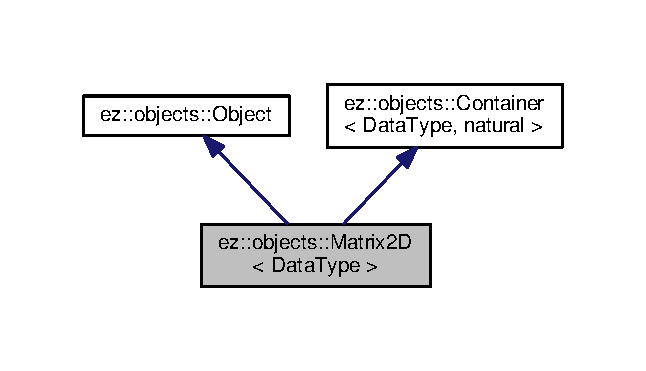
\includegraphics[width=310pt]{classez_1_1objects_1_1Matrix2D__inherit__graph}
\end{center}
\end{figure}


Collaboration diagram for ez\+:\+:objects\+:\+:Matrix2D$<$ Data\+Type $>$\+:
\nopagebreak
\begin{figure}[H]
\begin{center}
\leavevmode
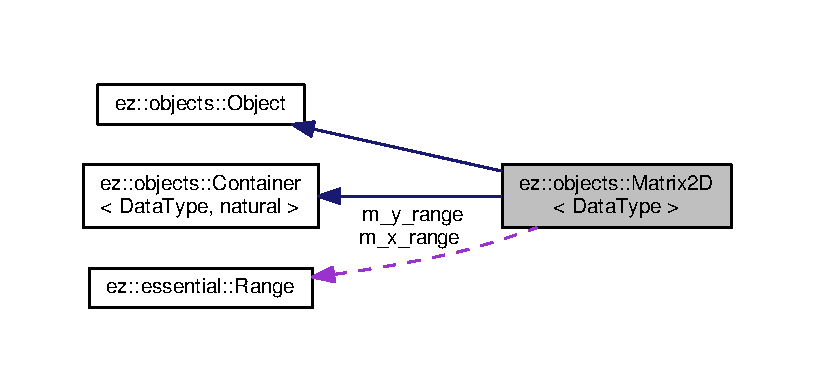
\includegraphics[width=350pt]{classez_1_1objects_1_1Matrix2D__coll__graph}
\end{center}
\end{figure}
\subsection*{Public Types}
\begin{DoxyCompactItemize}
\item 
\mbox{\Hypertarget{classez_1_1objects_1_1Matrix2D_aed7325d5d1ae52ffd652dc6f5424961a}\label{classez_1_1objects_1_1Matrix2D_aed7325d5d1ae52ffd652dc6f5424961a}} 
typedef \hyperlink{classez_1_1objects_1_1Matrix2D}{Matrix2D}$<$ Data\+Type $>$ {\bfseries self}
\item 
\mbox{\Hypertarget{classez_1_1objects_1_1Matrix2D_a0fc564d5a00d0145ca6b2986b797649b}\label{classez_1_1objects_1_1Matrix2D_a0fc564d5a00d0145ca6b2986b797649b}} 
typedef Data\+Type $\ast$ {\bfseries iterator}
\end{DoxyCompactItemize}
\subsection*{Public Member Functions}
\begin{DoxyCompactItemize}
\item 
\hyperlink{classez_1_1objects_1_1Matrix2D_a1984c0e18d3921f89edc9f255c7eef70}{Matrix2D} ()
\item 
\hyperlink{classez_1_1objects_1_1Matrix2D_ac3bd803c3d42ae0eeb0bc50d04148d7f}{Matrix2D} (\hyperlink{classez_1_1essential_1_1Range}{ez\+::essential\+::\+Range} y\+\_\+range, \hyperlink{classez_1_1essential_1_1Range}{ez\+::essential\+::\+Range} x\+\_\+range)
\item 
\hyperlink{classez_1_1objects_1_1Matrix2D_aa8e3f8149bc97efb0a2c45c10520594b}{Matrix2D} (\hyperlink{classez_1_1essential_1_1Range}{ez\+::essential\+::\+Range} y\+\_\+range, \hyperlink{classez_1_1essential_1_1Range}{ez\+::essential\+::\+Range} x\+\_\+range, const std\+::initializer\+\_\+list$<$ Data\+Type $>$ \&l)
\item 
\hyperlink{classez_1_1objects_1_1Matrix2D_aeebbde5d2059f7e190759dfc0412f353}{Matrix2D} (const \hyperlink{classez_1_1objects_1_1Matrix2D}{self} \&obj)
\item 
\hyperlink{classez_1_1objects_1_1Matrix2D}{self} \& \hyperlink{classez_1_1objects_1_1Matrix2D_a693a0c5feb9dd40f8a3f72abc7680f46}{operator=} (const \hyperlink{classez_1_1objects_1_1Matrix2D}{self} \&obj)
\item 
\hyperlink{classez_1_1objects_1_1Matrix2D_a3de573bc8beb0160ebb6bdfa7bf4daa2}{$\sim$\+Matrix2D} ()
\item 
void \hyperlink{classez_1_1objects_1_1Matrix2D_a14783b5e865959b2aa6d1b19ec705b37}{resize} (\hyperlink{classez_1_1essential_1_1Range}{ez\+::essential\+::\+Range} y\+\_\+range, \hyperlink{classez_1_1essential_1_1Range}{ez\+::essential\+::\+Range} x\+\_\+range)
\item 
natural \hyperlink{classez_1_1objects_1_1Matrix2D_a236462257912521cf98d8b5899f228f2}{size} ()
\item 
bool \hyperlink{classez_1_1objects_1_1Matrix2D_acab487d980231c63d1ea4dd6de734b2f}{is\+\_\+empty} ()
\item 
\mbox{\Hypertarget{classez_1_1objects_1_1Matrix2D_a3346b8cb727a77de4d6f21d7f1c8d828}\label{classez_1_1objects_1_1Matrix2D_a3346b8cb727a77de4d6f21d7f1c8d828}} 
\hyperlink{classez_1_1essential_1_1Range}{ez\+::essential\+::\+Range} \& {\bfseries x\+\_\+range} ()
\item 
\mbox{\Hypertarget{classez_1_1objects_1_1Matrix2D_a0358977f3d99b47af02fca8b2c9ae698}\label{classez_1_1objects_1_1Matrix2D_a0358977f3d99b47af02fca8b2c9ae698}} 
\hyperlink{classez_1_1essential_1_1Range}{ez\+::essential\+::\+Range} \& {\bfseries y\+\_\+range} ()
\item 
Data\+Type \& \hyperlink{classez_1_1objects_1_1Matrix2D_a43445a3d46105c71f6e212c2b996bced}{get} (int y, int x)
\item 
\mbox{\Hypertarget{classez_1_1objects_1_1Matrix2D_a6191b365c96c388d82d7a205f979a30e}\label{classez_1_1objects_1_1Matrix2D_a6191b365c96c388d82d7a205f979a30e}} 
Data\+Type \& {\bfseries operator()} (int y, int x)
\item 
\mbox{\Hypertarget{classez_1_1objects_1_1Matrix2D_ab733a21ed5cb3ad3980c15af20ec066a}\label{classez_1_1objects_1_1Matrix2D_ab733a21ed5cb3ad3980c15af20ec066a}} 
void {\bfseries put} (int y, int x, Data\+Type value)
\item 
void \hyperlink{classez_1_1objects_1_1Matrix2D_aeef806111fdd458dfcf1f09addd7a0b7}{print} (std\+::ostream \&stream)
\item 
integer \hyperlink{classez_1_1objects_1_1Matrix2D_ab0b55556ba7c31aa5ad376a91b63d6c3}{compare} (const \hyperlink{classez_1_1objects_1_1Object}{Object} \&y) override
\item 
\mbox{\Hypertarget{classez_1_1objects_1_1Matrix2D_addb8a79fde0fbdf234ffaac900218ad6}\label{classez_1_1objects_1_1Matrix2D_addb8a79fde0fbdf234ffaac900218ad6}} 
iterator {\bfseries begin} ()
\item 
\mbox{\Hypertarget{classez_1_1objects_1_1Matrix2D_a327f80adc9100fa1f8e484727e970aef}\label{classez_1_1objects_1_1Matrix2D_a327f80adc9100fa1f8e484727e970aef}} 
iterator {\bfseries end} ()
\item 
\mbox{\Hypertarget{classez_1_1objects_1_1Matrix2D_adfe8ae81d04a641df8ec9e7fde7fb622}\label{classez_1_1objects_1_1Matrix2D_adfe8ae81d04a641df8ec9e7fde7fb622}} 
void {\bfseries fill\+\_\+column} (int x, Data\+Type value)
\item 
\mbox{\Hypertarget{classez_1_1objects_1_1Matrix2D_aea80758870a92d991ddf71ce15fd254b}\label{classez_1_1objects_1_1Matrix2D_aea80758870a92d991ddf71ce15fd254b}} 
void {\bfseries fill\+\_\+row} (int y, Data\+Type value)
\item 
\mbox{\Hypertarget{classez_1_1objects_1_1Matrix2D_a5e6110ccfbdd8b85e122113b5a347f8e}\label{classez_1_1objects_1_1Matrix2D_a5e6110ccfbdd8b85e122113b5a347f8e}} 
void {\bfseries get\+\_\+column} (int x, \hyperlink{classez_1_1objects_1_1Array}{Array}$<$ Data\+Type $>$ \&a)
\item 
\mbox{\Hypertarget{classez_1_1objects_1_1Matrix2D_a8605f64c49804d7364603d47b4e44151}\label{classez_1_1objects_1_1Matrix2D_a8605f64c49804d7364603d47b4e44151}} 
void {\bfseries get\+\_\+row} (int y, \hyperlink{classez_1_1objects_1_1Array}{Array}$<$ Data\+Type $>$ \&a)
\item 
\mbox{\Hypertarget{classez_1_1objects_1_1Matrix2D_af29b41746bb0bcf4dce2c19c48621352}\label{classez_1_1objects_1_1Matrix2D_af29b41746bb0bcf4dce2c19c48621352}} 
void {\bfseries transpose} ()
\end{DoxyCompactItemize}
\subsection*{Protected Attributes}
\begin{DoxyCompactItemize}
\item 
\mbox{\Hypertarget{classez_1_1objects_1_1Matrix2D_ac62730b69c28de172d72e7af57086439}\label{classez_1_1objects_1_1Matrix2D_ac62730b69c28de172d72e7af57086439}} 
\hyperlink{classez_1_1essential_1_1Range}{ez\+::essential\+::\+Range} {\bfseries m\+\_\+x\+\_\+range}
\item 
\mbox{\Hypertarget{classez_1_1objects_1_1Matrix2D_a0f4f1ece5e7d2f725fea3d29a4ca4ae8}\label{classez_1_1objects_1_1Matrix2D_a0f4f1ece5e7d2f725fea3d29a4ca4ae8}} 
\hyperlink{classez_1_1essential_1_1Range}{ez\+::essential\+::\+Range} {\bfseries m\+\_\+y\+\_\+range}
\item 
\mbox{\Hypertarget{classez_1_1objects_1_1Matrix2D_a044af0f88f186c25326018f1e1c19017}\label{classez_1_1objects_1_1Matrix2D_a044af0f88f186c25326018f1e1c19017}} 
natural {\bfseries m\+\_\+x\+\_\+size}
\item 
\mbox{\Hypertarget{classez_1_1objects_1_1Matrix2D_a34b6f7d68b6f47c05ef6aeb2e9dee189}\label{classez_1_1objects_1_1Matrix2D_a34b6f7d68b6f47c05ef6aeb2e9dee189}} 
natural {\bfseries m\+\_\+size}
\item 
\mbox{\Hypertarget{classez_1_1objects_1_1Matrix2D_a73b7ae54bdc47648c5fb0b2ce5cab2cb}\label{classez_1_1objects_1_1Matrix2D_a73b7ae54bdc47648c5fb0b2ce5cab2cb}} 
Data\+Type $\ast$ {\bfseries m\+\_\+data}
\end{DoxyCompactItemize}
\subsection*{Additional Inherited Members}


\subsection{Constructor \& Destructor Documentation}
\mbox{\Hypertarget{classez_1_1objects_1_1Matrix2D_a1984c0e18d3921f89edc9f255c7eef70}\label{classez_1_1objects_1_1Matrix2D_a1984c0e18d3921f89edc9f255c7eef70}} 
\index{ez\+::objects\+::\+Matrix2D@{ez\+::objects\+::\+Matrix2D}!Matrix2D@{Matrix2D}}
\index{Matrix2D@{Matrix2D}!ez\+::objects\+::\+Matrix2D@{ez\+::objects\+::\+Matrix2D}}
\subsubsection{\texorpdfstring{Matrix2\+D()}{Matrix2D()}\hspace{0.1cm}{\footnotesize\ttfamily [1/4]}}
{\footnotesize\ttfamily template$<$class Data\+Type $>$ \\
\hyperlink{classez_1_1objects_1_1Matrix2D}{ez\+::objects\+::\+Matrix2D}$<$ Data\+Type $>$\+::\hyperlink{classez_1_1objects_1_1Matrix2D}{Matrix2D} (\begin{DoxyParamCaption}{ }\end{DoxyParamCaption})\hspace{0.3cm}{\ttfamily [inline]}}

Default constructor \mbox{\Hypertarget{classez_1_1objects_1_1Matrix2D_ac3bd803c3d42ae0eeb0bc50d04148d7f}\label{classez_1_1objects_1_1Matrix2D_ac3bd803c3d42ae0eeb0bc50d04148d7f}} 
\index{ez\+::objects\+::\+Matrix2D@{ez\+::objects\+::\+Matrix2D}!Matrix2D@{Matrix2D}}
\index{Matrix2D@{Matrix2D}!ez\+::objects\+::\+Matrix2D@{ez\+::objects\+::\+Matrix2D}}
\subsubsection{\texorpdfstring{Matrix2\+D()}{Matrix2D()}\hspace{0.1cm}{\footnotesize\ttfamily [2/4]}}
{\footnotesize\ttfamily template$<$class Data\+Type $>$ \\
\hyperlink{classez_1_1objects_1_1Matrix2D}{ez\+::objects\+::\+Matrix2D}$<$ Data\+Type $>$\+::\hyperlink{classez_1_1objects_1_1Matrix2D}{Matrix2D} (\begin{DoxyParamCaption}\item[{\hyperlink{classez_1_1essential_1_1Range}{ez\+::essential\+::\+Range}}]{y\+\_\+range,  }\item[{\hyperlink{classez_1_1essential_1_1Range}{ez\+::essential\+::\+Range}}]{x\+\_\+range }\end{DoxyParamCaption})\hspace{0.3cm}{\ttfamily [inline]}}

Constructor given row and column range \mbox{\Hypertarget{classez_1_1objects_1_1Matrix2D_aa8e3f8149bc97efb0a2c45c10520594b}\label{classez_1_1objects_1_1Matrix2D_aa8e3f8149bc97efb0a2c45c10520594b}} 
\index{ez\+::objects\+::\+Matrix2D@{ez\+::objects\+::\+Matrix2D}!Matrix2D@{Matrix2D}}
\index{Matrix2D@{Matrix2D}!ez\+::objects\+::\+Matrix2D@{ez\+::objects\+::\+Matrix2D}}
\subsubsection{\texorpdfstring{Matrix2\+D()}{Matrix2D()}\hspace{0.1cm}{\footnotesize\ttfamily [3/4]}}
{\footnotesize\ttfamily template$<$class Data\+Type $>$ \\
\hyperlink{classez_1_1objects_1_1Matrix2D}{ez\+::objects\+::\+Matrix2D}$<$ Data\+Type $>$\+::\hyperlink{classez_1_1objects_1_1Matrix2D}{Matrix2D} (\begin{DoxyParamCaption}\item[{\hyperlink{classez_1_1essential_1_1Range}{ez\+::essential\+::\+Range}}]{y\+\_\+range,  }\item[{\hyperlink{classez_1_1essential_1_1Range}{ez\+::essential\+::\+Range}}]{x\+\_\+range,  }\item[{const std\+::initializer\+\_\+list$<$ Data\+Type $>$ \&}]{l }\end{DoxyParamCaption})\hspace{0.3cm}{\ttfamily [inline]}}

Constructor given row and column range and list of values \mbox{\Hypertarget{classez_1_1objects_1_1Matrix2D_aeebbde5d2059f7e190759dfc0412f353}\label{classez_1_1objects_1_1Matrix2D_aeebbde5d2059f7e190759dfc0412f353}} 
\index{ez\+::objects\+::\+Matrix2D@{ez\+::objects\+::\+Matrix2D}!Matrix2D@{Matrix2D}}
\index{Matrix2D@{Matrix2D}!ez\+::objects\+::\+Matrix2D@{ez\+::objects\+::\+Matrix2D}}
\subsubsection{\texorpdfstring{Matrix2\+D()}{Matrix2D()}\hspace{0.1cm}{\footnotesize\ttfamily [4/4]}}
{\footnotesize\ttfamily template$<$class Data\+Type $>$ \\
\hyperlink{classez_1_1objects_1_1Matrix2D}{ez\+::objects\+::\+Matrix2D}$<$ Data\+Type $>$\+::\hyperlink{classez_1_1objects_1_1Matrix2D}{Matrix2D} (\begin{DoxyParamCaption}\item[{const \hyperlink{classez_1_1objects_1_1Matrix2D}{self} \&}]{obj }\end{DoxyParamCaption})\hspace{0.3cm}{\ttfamily [inline]}}

Copy constructor \mbox{\Hypertarget{classez_1_1objects_1_1Matrix2D_a3de573bc8beb0160ebb6bdfa7bf4daa2}\label{classez_1_1objects_1_1Matrix2D_a3de573bc8beb0160ebb6bdfa7bf4daa2}} 
\index{ez\+::objects\+::\+Matrix2D@{ez\+::objects\+::\+Matrix2D}!````~Matrix2D@{$\sim$\+Matrix2D}}
\index{````~Matrix2D@{$\sim$\+Matrix2D}!ez\+::objects\+::\+Matrix2D@{ez\+::objects\+::\+Matrix2D}}
\subsubsection{\texorpdfstring{$\sim$\+Matrix2\+D()}{~Matrix2D()}}
{\footnotesize\ttfamily template$<$class Data\+Type $>$ \\
\hyperlink{classez_1_1objects_1_1Matrix2D}{ez\+::objects\+::\+Matrix2D}$<$ Data\+Type $>$\+::$\sim$\hyperlink{classez_1_1objects_1_1Matrix2D}{Matrix2D} (\begin{DoxyParamCaption}{ }\end{DoxyParamCaption})\hspace{0.3cm}{\ttfamily [inline]}}

Destructor 

\subsection{Member Function Documentation}
\mbox{\Hypertarget{classez_1_1objects_1_1Matrix2D_ab0b55556ba7c31aa5ad376a91b63d6c3}\label{classez_1_1objects_1_1Matrix2D_ab0b55556ba7c31aa5ad376a91b63d6c3}} 
\index{ez\+::objects\+::\+Matrix2D@{ez\+::objects\+::\+Matrix2D}!compare@{compare}}
\index{compare@{compare}!ez\+::objects\+::\+Matrix2D@{ez\+::objects\+::\+Matrix2D}}
\subsubsection{\texorpdfstring{compare()}{compare()}}
{\footnotesize\ttfamily template$<$class Data\+Type $>$ \\
integer \hyperlink{classez_1_1objects_1_1Matrix2D}{ez\+::objects\+::\+Matrix2D}$<$ Data\+Type $>$\+::compare (\begin{DoxyParamCaption}\item[{const \hyperlink{classez_1_1objects_1_1Object}{Object} \&}]{y }\end{DoxyParamCaption})\hspace{0.3cm}{\ttfamily [inline]}, {\ttfamily [override]}, {\ttfamily [virtual]}}

compare two objects \begin{DoxyReturn}{Returns}
0 if objects are identical, negative value if this $<$ y, positive value if this $>$ y 
\end{DoxyReturn}


Reimplemented from \hyperlink{classez_1_1objects_1_1Object_aca311d389dffa204e425463145f4e1e6}{ez\+::objects\+::\+Object}.

\mbox{\Hypertarget{classez_1_1objects_1_1Matrix2D_a43445a3d46105c71f6e212c2b996bced}\label{classez_1_1objects_1_1Matrix2D_a43445a3d46105c71f6e212c2b996bced}} 
\index{ez\+::objects\+::\+Matrix2D@{ez\+::objects\+::\+Matrix2D}!get@{get}}
\index{get@{get}!ez\+::objects\+::\+Matrix2D@{ez\+::objects\+::\+Matrix2D}}
\subsubsection{\texorpdfstring{get()}{get()}}
{\footnotesize\ttfamily template$<$class Data\+Type $>$ \\
Data\+Type\& \hyperlink{classez_1_1objects_1_1Matrix2D}{ez\+::objects\+::\+Matrix2D}$<$ Data\+Type $>$\+::get (\begin{DoxyParamCaption}\item[{int}]{y,  }\item[{int}]{x }\end{DoxyParamCaption})\hspace{0.3cm}{\ttfamily [inline]}}

get value at given row and column and check if coordinates are in the allowed ranges. 
\begin{DoxyParams}{Parameters}
{\em y} & row identification \\
\hline
{\em x} & column identification \\
\hline
\end{DoxyParams}
\mbox{\Hypertarget{classez_1_1objects_1_1Matrix2D_acab487d980231c63d1ea4dd6de734b2f}\label{classez_1_1objects_1_1Matrix2D_acab487d980231c63d1ea4dd6de734b2f}} 
\index{ez\+::objects\+::\+Matrix2D@{ez\+::objects\+::\+Matrix2D}!is\+\_\+empty@{is\+\_\+empty}}
\index{is\+\_\+empty@{is\+\_\+empty}!ez\+::objects\+::\+Matrix2D@{ez\+::objects\+::\+Matrix2D}}
\subsubsection{\texorpdfstring{is\+\_\+empty()}{is\_empty()}}
{\footnotesize\ttfamily template$<$class Data\+Type $>$ \\
bool \hyperlink{classez_1_1objects_1_1Matrix2D}{ez\+::objects\+::\+Matrix2D}$<$ Data\+Type $>$\+::is\+\_\+empty (\begin{DoxyParamCaption}{ }\end{DoxyParamCaption})\hspace{0.3cm}{\ttfamily [inline]}, {\ttfamily [virtual]}}

Return true if container has no element, false otherwise 

Implements \hyperlink{classez_1_1objects_1_1Container_a205eb4f8a4fe967d425fdf04e5db5f93}{ez\+::objects\+::\+Container$<$ Data\+Type, natural $>$}.

\mbox{\Hypertarget{classez_1_1objects_1_1Matrix2D_a693a0c5feb9dd40f8a3f72abc7680f46}\label{classez_1_1objects_1_1Matrix2D_a693a0c5feb9dd40f8a3f72abc7680f46}} 
\index{ez\+::objects\+::\+Matrix2D@{ez\+::objects\+::\+Matrix2D}!operator=@{operator=}}
\index{operator=@{operator=}!ez\+::objects\+::\+Matrix2D@{ez\+::objects\+::\+Matrix2D}}
\subsubsection{\texorpdfstring{operator=()}{operator=()}}
{\footnotesize\ttfamily template$<$class Data\+Type $>$ \\
\hyperlink{classez_1_1objects_1_1Matrix2D}{self}\& \hyperlink{classez_1_1objects_1_1Matrix2D}{ez\+::objects\+::\+Matrix2D}$<$ Data\+Type $>$\+::operator= (\begin{DoxyParamCaption}\item[{const \hyperlink{classez_1_1objects_1_1Matrix2D}{self} \&}]{obj }\end{DoxyParamCaption})\hspace{0.3cm}{\ttfamily [inline]}}

Overloading of assignment operator \mbox{\Hypertarget{classez_1_1objects_1_1Matrix2D_aeef806111fdd458dfcf1f09addd7a0b7}\label{classez_1_1objects_1_1Matrix2D_aeef806111fdd458dfcf1f09addd7a0b7}} 
\index{ez\+::objects\+::\+Matrix2D@{ez\+::objects\+::\+Matrix2D}!print@{print}}
\index{print@{print}!ez\+::objects\+::\+Matrix2D@{ez\+::objects\+::\+Matrix2D}}
\subsubsection{\texorpdfstring{print()}{print()}}
{\footnotesize\ttfamily template$<$class Data\+Type $>$ \\
void \hyperlink{classez_1_1objects_1_1Matrix2D}{ez\+::objects\+::\+Matrix2D}$<$ Data\+Type $>$\+::print (\begin{DoxyParamCaption}\item[{std\+::ostream \&}]{stream }\end{DoxyParamCaption})\hspace{0.3cm}{\ttfamily [inline]}, {\ttfamily [virtual]}}

this function is used to print the contents of the object in a human readable format 
\begin{DoxyParams}{Parameters}
{\em stream} & output stream for example std\+::cout \\
\hline
\end{DoxyParams}


Reimplemented from \hyperlink{classez_1_1objects_1_1Object_a9e20f39a78163f67f000576149d858b3}{ez\+::objects\+::\+Object}.

\mbox{\Hypertarget{classez_1_1objects_1_1Matrix2D_a14783b5e865959b2aa6d1b19ec705b37}\label{classez_1_1objects_1_1Matrix2D_a14783b5e865959b2aa6d1b19ec705b37}} 
\index{ez\+::objects\+::\+Matrix2D@{ez\+::objects\+::\+Matrix2D}!resize@{resize}}
\index{resize@{resize}!ez\+::objects\+::\+Matrix2D@{ez\+::objects\+::\+Matrix2D}}
\subsubsection{\texorpdfstring{resize()}{resize()}}
{\footnotesize\ttfamily template$<$class Data\+Type $>$ \\
void \hyperlink{classez_1_1objects_1_1Matrix2D}{ez\+::objects\+::\+Matrix2D}$<$ Data\+Type $>$\+::resize (\begin{DoxyParamCaption}\item[{\hyperlink{classez_1_1essential_1_1Range}{ez\+::essential\+::\+Range}}]{y\+\_\+range,  }\item[{\hyperlink{classez_1_1essential_1_1Range}{ez\+::essential\+::\+Range}}]{x\+\_\+range }\end{DoxyParamCaption})\hspace{0.3cm}{\ttfamily [inline]}}

Resize container \mbox{\Hypertarget{classez_1_1objects_1_1Matrix2D_a236462257912521cf98d8b5899f228f2}\label{classez_1_1objects_1_1Matrix2D_a236462257912521cf98d8b5899f228f2}} 
\index{ez\+::objects\+::\+Matrix2D@{ez\+::objects\+::\+Matrix2D}!size@{size}}
\index{size@{size}!ez\+::objects\+::\+Matrix2D@{ez\+::objects\+::\+Matrix2D}}
\subsubsection{\texorpdfstring{size()}{size()}}
{\footnotesize\ttfamily template$<$class Data\+Type $>$ \\
natural \hyperlink{classez_1_1objects_1_1Matrix2D}{ez\+::objects\+::\+Matrix2D}$<$ Data\+Type $>$\+::size (\begin{DoxyParamCaption}{ }\end{DoxyParamCaption})\hspace{0.3cm}{\ttfamily [inline]}, {\ttfamily [virtual]}}

Return size of container 

Implements \hyperlink{classez_1_1objects_1_1Container_affd294810c6c29530d1d1e3c2151ad28}{ez\+::objects\+::\+Container$<$ Data\+Type, natural $>$}.



The documentation for this class was generated from the following files\+:\begin{DoxyCompactItemize}
\item 
src/version\+\_\+2018.\+06/objects/array.\+h\item 
src/version\+\_\+2018.\+06/objects/matrix2d.\+h\end{DoxyCompactItemize}

\hypertarget{classez_1_1objects_1_1Matrix3D}{}\section{ez\+:\+:objects\+:\+:Matrix3D$<$ Data\+Type $>$ Class Template Reference}
\label{classez_1_1objects_1_1Matrix3D}\index{ez\+::objects\+::\+Matrix3\+D$<$ Data\+Type $>$@{ez\+::objects\+::\+Matrix3\+D$<$ Data\+Type $>$}}


Inheritance diagram for ez\+:\+:objects\+:\+:Matrix3D$<$ Data\+Type $>$\+:
\nopagebreak
\begin{figure}[H]
\begin{center}
\leavevmode
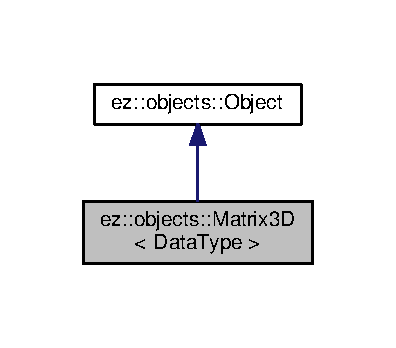
\includegraphics[width=190pt]{classez_1_1objects_1_1Matrix3D__inherit__graph}
\end{center}
\end{figure}


Collaboration diagram for ez\+:\+:objects\+:\+:Matrix3D$<$ Data\+Type $>$\+:
\nopagebreak
\begin{figure}[H]
\begin{center}
\leavevmode
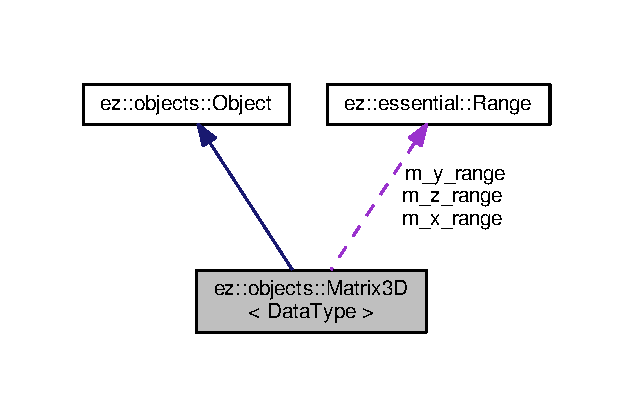
\includegraphics[width=304pt]{classez_1_1objects_1_1Matrix3D__coll__graph}
\end{center}
\end{figure}
\subsection*{Public Types}
\begin{DoxyCompactItemize}
\item 
\mbox{\Hypertarget{classez_1_1objects_1_1Matrix3D_a5a17da6e4dc5af4923219ce71c8790c8}\label{classez_1_1objects_1_1Matrix3D_a5a17da6e4dc5af4923219ce71c8790c8}} 
typedef \hyperlink{classez_1_1objects_1_1Matrix2D}{Matrix2D}$<$ Data\+Type $>$ {\bfseries self}
\item 
\mbox{\Hypertarget{classez_1_1objects_1_1Matrix3D_abcdbe37fb87dbfb21149eb2105cd94df}\label{classez_1_1objects_1_1Matrix3D_abcdbe37fb87dbfb21149eb2105cd94df}} 
typedef Data\+Type $\ast$ {\bfseries iterator}
\end{DoxyCompactItemize}
\subsection*{Public Member Functions}
\begin{DoxyCompactItemize}
\item 
\mbox{\Hypertarget{classez_1_1objects_1_1Matrix3D_a4c811f58573ac9d4e6734a661040610d}\label{classez_1_1objects_1_1Matrix3D_a4c811f58573ac9d4e6734a661040610d}} 
{\bfseries Matrix3D} (\hyperlink{classez_1_1essential_1_1Range}{ez\+::essential\+::\+Range} x\+\_\+range, \hyperlink{classez_1_1essential_1_1Range}{ez\+::essential\+::\+Range} y\+\_\+range, \hyperlink{classez_1_1essential_1_1Range}{ez\+::essential\+::\+Range} z\+\_\+range)
\item 
\mbox{\Hypertarget{classez_1_1objects_1_1Matrix3D_a9c59c894cd089e7df30e898825608159}\label{classez_1_1objects_1_1Matrix3D_a9c59c894cd089e7df30e898825608159}} 
{\bfseries Matrix3D} (const \hyperlink{classez_1_1objects_1_1Matrix2D}{self} \&obj)
\item 
\mbox{\Hypertarget{classez_1_1objects_1_1Matrix3D_a57c03371c577f882b6c3d44c10d681da}\label{classez_1_1objects_1_1Matrix3D_a57c03371c577f882b6c3d44c10d681da}} 
\hyperlink{classez_1_1objects_1_1Matrix2D}{self} \& {\bfseries operator=} (const \hyperlink{classez_1_1objects_1_1Matrix2D}{self} \&obj)
\item 
\mbox{\Hypertarget{classez_1_1objects_1_1Matrix3D_ad1ea1261c73a0d24d03e2511c01e1ec8}\label{classez_1_1objects_1_1Matrix3D_ad1ea1261c73a0d24d03e2511c01e1ec8}} 
void {\bfseries resize} (\hyperlink{classez_1_1essential_1_1Range}{ez\+::essential\+::\+Range} x\+\_\+range, \hyperlink{classez_1_1essential_1_1Range}{ez\+::essential\+::\+Range} y\+\_\+range, \hyperlink{classez_1_1essential_1_1Range}{ez\+::essential\+::\+Range} z\+\_\+range)
\item 
\mbox{\Hypertarget{classez_1_1objects_1_1Matrix3D_af5488d52918f0f34f9cfffe8ed604b70}\label{classez_1_1objects_1_1Matrix3D_af5488d52918f0f34f9cfffe8ed604b70}} 
natural {\bfseries size} ()
\item 
\mbox{\Hypertarget{classez_1_1objects_1_1Matrix3D_abcaf2e884ff6322ea00b111eb7f1144f}\label{classez_1_1objects_1_1Matrix3D_abcaf2e884ff6322ea00b111eb7f1144f}} 
Data\+Type \& {\bfseries safe\+\_\+get} (int x, int y, int z)
\item 
\mbox{\Hypertarget{classez_1_1objects_1_1Matrix3D_a1d88a788f1f065f9dbfc5ca80ea8c7ae}\label{classez_1_1objects_1_1Matrix3D_a1d88a788f1f065f9dbfc5ca80ea8c7ae}} 
Data\+Type \& {\bfseries get} (int x, int y, int z)
\item 
\mbox{\Hypertarget{classez_1_1objects_1_1Matrix3D_a01be5d7137b0e505f23b98b9ead84fc7}\label{classez_1_1objects_1_1Matrix3D_a01be5d7137b0e505f23b98b9ead84fc7}} 
void {\bfseries safe\+\_\+put} (int x, int y, int z, Data\+Type value)
\item 
\mbox{\Hypertarget{classez_1_1objects_1_1Matrix3D_aac440ad88f5346e5d10f9f1ae53f4bf6}\label{classez_1_1objects_1_1Matrix3D_aac440ad88f5346e5d10f9f1ae53f4bf6}} 
void {\bfseries put} (int x, int y, int z, Data\+Type value)
\item 
void \hyperlink{classez_1_1objects_1_1Matrix3D_a5e68194ecbc90039bf694377a579b59c}{print} (std\+::ostream \&stream)
\item 
\mbox{\Hypertarget{classez_1_1objects_1_1Matrix3D_a8f7565cbeff933a77c6a418a1ef33de7}\label{classez_1_1objects_1_1Matrix3D_a8f7565cbeff933a77c6a418a1ef33de7}} 
iterator {\bfseries begin} ()
\item 
\mbox{\Hypertarget{classez_1_1objects_1_1Matrix3D_a4455fc86c241687009196f983994ddf5}\label{classez_1_1objects_1_1Matrix3D_a4455fc86c241687009196f983994ddf5}} 
iterator {\bfseries end} ()
\end{DoxyCompactItemize}
\subsection*{Data Fields}
\begin{DoxyCompactItemize}
\item 
\mbox{\Hypertarget{classez_1_1objects_1_1Matrix3D_a0544904c21295ea452d0e0180db3e41f}\label{classez_1_1objects_1_1Matrix3D_a0544904c21295ea452d0e0180db3e41f}} 
\hyperlink{classez_1_1essential_1_1Range}{ez\+::essential\+::\+Range} {\bfseries m\+\_\+x\+\_\+range}
\item 
\mbox{\Hypertarget{classez_1_1objects_1_1Matrix3D_add280dfed8a17e70a78d34caea7e9cf2}\label{classez_1_1objects_1_1Matrix3D_add280dfed8a17e70a78d34caea7e9cf2}} 
\hyperlink{classez_1_1essential_1_1Range}{ez\+::essential\+::\+Range} {\bfseries m\+\_\+y\+\_\+range}
\item 
\mbox{\Hypertarget{classez_1_1objects_1_1Matrix3D_a06da3c5d6d3f37b7edb5958cce62f679}\label{classez_1_1objects_1_1Matrix3D_a06da3c5d6d3f37b7edb5958cce62f679}} 
\hyperlink{classez_1_1essential_1_1Range}{ez\+::essential\+::\+Range} {\bfseries m\+\_\+z\+\_\+range}
\item 
\mbox{\Hypertarget{classez_1_1objects_1_1Matrix3D_a58ae013adbf48027f42590ecdb668b60}\label{classez_1_1objects_1_1Matrix3D_a58ae013adbf48027f42590ecdb668b60}} 
natural {\bfseries m\+\_\+x\+\_\+size}
\item 
\mbox{\Hypertarget{classez_1_1objects_1_1Matrix3D_a529b9fe5dad9cf31f0a3a2169f194247}\label{classez_1_1objects_1_1Matrix3D_a529b9fe5dad9cf31f0a3a2169f194247}} 
natural {\bfseries m\+\_\+xy\+\_\+size}
\item 
\mbox{\Hypertarget{classez_1_1objects_1_1Matrix3D_a03de23a09ae91fcdc5b65408d280e3c9}\label{classez_1_1objects_1_1Matrix3D_a03de23a09ae91fcdc5b65408d280e3c9}} 
natural {\bfseries m\+\_\+size}
\item 
\mbox{\Hypertarget{classez_1_1objects_1_1Matrix3D_a292ada7dbe95708f68c757cdf36a5a56}\label{classez_1_1objects_1_1Matrix3D_a292ada7dbe95708f68c757cdf36a5a56}} 
Data\+Type $\ast$ {\bfseries m\+\_\+data}
\end{DoxyCompactItemize}
\subsection*{Additional Inherited Members}


\subsection{Member Function Documentation}
\mbox{\Hypertarget{classez_1_1objects_1_1Matrix3D_a5e68194ecbc90039bf694377a579b59c}\label{classez_1_1objects_1_1Matrix3D_a5e68194ecbc90039bf694377a579b59c}} 
\index{ez\+::objects\+::\+Matrix3D@{ez\+::objects\+::\+Matrix3D}!print@{print}}
\index{print@{print}!ez\+::objects\+::\+Matrix3D@{ez\+::objects\+::\+Matrix3D}}
\subsubsection{\texorpdfstring{print()}{print()}}
{\footnotesize\ttfamily template$<$class Data\+Type $>$ \\
void \hyperlink{classez_1_1objects_1_1Matrix3D}{ez\+::objects\+::\+Matrix3D}$<$ Data\+Type $>$\+::print (\begin{DoxyParamCaption}\item[{std\+::ostream \&}]{stream }\end{DoxyParamCaption})\hspace{0.3cm}{\ttfamily [inline]}, {\ttfamily [virtual]}}

this function is used to print the contents of the object in a human readable format 
\begin{DoxyParams}{Parameters}
{\em stream} & output stream for example std\+::cout \\
\hline
\end{DoxyParams}


Reimplemented from \hyperlink{classez_1_1objects_1_1Object_a9e20f39a78163f67f000576149d858b3}{ez\+::objects\+::\+Object}.



The documentation for this class was generated from the following file\+:\begin{DoxyCompactItemize}
\item 
src/version\+\_\+2018.\+06/objects/matrix3d.\+h\end{DoxyCompactItemize}

\hypertarget{classez_1_1maths_1_1Matrix_1_1MatrixRow}{}\section{ez\+:\+:maths\+:\+:Matrix$<$ Data\+Type $>$\+:\+:Matrix\+Row Class Reference}
\label{classez_1_1maths_1_1Matrix_1_1MatrixRow}\index{ez\+::maths\+::\+Matrix$<$ Data\+Type $>$\+::\+Matrix\+Row@{ez\+::maths\+::\+Matrix$<$ Data\+Type $>$\+::\+Matrix\+Row}}
\subsection*{Public Member Functions}
\begin{DoxyCompactItemize}
\item 
\mbox{\Hypertarget{classez_1_1maths_1_1Matrix_1_1MatrixRow_a55fa07c1bfe2d6e13be70c051ba5cc52}\label{classez_1_1maths_1_1Matrix_1_1MatrixRow_a55fa07c1bfe2d6e13be70c051ba5cc52}} 
{\bfseries Matrix\+Row} (std\+::vector$<$ Data\+Type $>$ \&row, natural y, natural size\+\_\+x)
\item 
\mbox{\Hypertarget{classez_1_1maths_1_1Matrix_1_1MatrixRow_a97aac7ce8b5b0f5f0f5a7e201649fcf2}\label{classez_1_1maths_1_1Matrix_1_1MatrixRow_a97aac7ce8b5b0f5f0f5a7e201649fcf2}} 
Data\+Type \& {\bfseries operator\mbox{[}$\,$\mbox{]}} (natural x)
\end{DoxyCompactItemize}


The documentation for this class was generated from the following file\+:\begin{DoxyCompactItemize}
\item 
src/version\+\_\+2018.\+06/maths/matrix.\+h\end{DoxyCompactItemize}

\hypertarget{classez_1_1logging_1_1MemoryLogger}{}\section{ez\+:\+:logging\+:\+:Memory\+Logger Class Reference}
\label{classez_1_1logging_1_1MemoryLogger}\index{ez\+::logging\+::\+Memory\+Logger@{ez\+::logging\+::\+Memory\+Logger}}


{\ttfamily \#include $<$logger.\+h$>$}



Inheritance diagram for ez\+:\+:logging\+:\+:Memory\+Logger\+:
\nopagebreak
\begin{figure}[H]
\begin{center}
\leavevmode
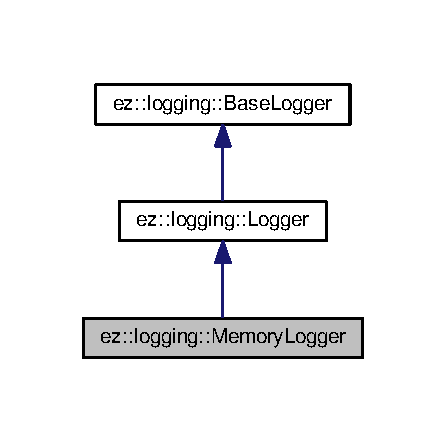
\includegraphics[width=214pt]{classez_1_1logging_1_1MemoryLogger__inherit__graph}
\end{center}
\end{figure}


Collaboration diagram for ez\+:\+:logging\+:\+:Memory\+Logger\+:
\nopagebreak
\begin{figure}[H]
\begin{center}
\leavevmode
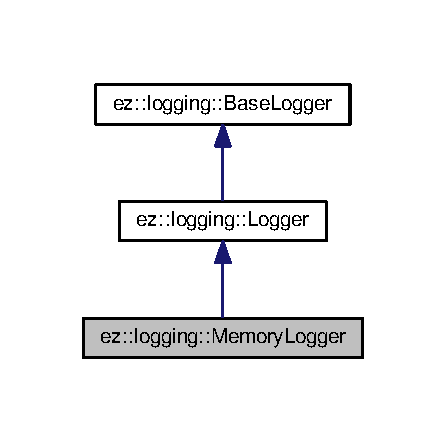
\includegraphics[width=214pt]{classez_1_1logging_1_1MemoryLogger__coll__graph}
\end{center}
\end{figure}
\subsection*{Public Member Functions}
\begin{DoxyCompactItemize}
\item 
\hyperlink{classez_1_1logging_1_1MemoryLogger_a721c1b62885a86e68819cb931c925f75}{Memory\+Logger} (std\+::string name)
\item 
\hyperlink{classez_1_1logging_1_1MemoryLogger_a421c0b502e122f86d5c5fbfa1660d6ee}{$\sim$\+Memory\+Logger} ()
\item 
std\+::string \hyperlink{classez_1_1logging_1_1MemoryLogger_aa4f77cc6ac0e272ce749b9bb4b939840}{get\+\_\+contents} ()
\item 
void \hyperlink{classez_1_1logging_1_1MemoryLogger_afa6c630d5e6334495f05727cdb7c3b16}{clear} ()
\item 
\mbox{\Hypertarget{classez_1_1logging_1_1MemoryLogger_a31cc1a88c8ee64447268ce7f46b042a1}\label{classez_1_1logging_1_1MemoryLogger_a31cc1a88c8ee64447268ce7f46b042a1}} 
\hyperlink{classez_1_1logging_1_1MemoryLogger}{Memory\+Logger} \& {\bfseries operator$<$$<$} (std\+::string \&s)
\end{DoxyCompactItemize}
\subsection*{Protected Attributes}
\begin{DoxyCompactItemize}
\item 
std\+::ostringstream \hyperlink{classez_1_1logging_1_1MemoryLogger_a45fc2a111c72be27408aef6c7a466dc0}{m\+\_\+output\+\_\+stream}
\end{DoxyCompactItemize}
\subsection*{Additional Inherited Members}


\subsection{Detailed Description}
\hyperlink{classez_1_1logging_1_1Logger}{Logger} for which information is kept in memory 

\subsection{Constructor \& Destructor Documentation}
\mbox{\Hypertarget{classez_1_1logging_1_1MemoryLogger_a721c1b62885a86e68819cb931c925f75}\label{classez_1_1logging_1_1MemoryLogger_a721c1b62885a86e68819cb931c925f75}} 
\index{ez\+::logging\+::\+Memory\+Logger@{ez\+::logging\+::\+Memory\+Logger}!Memory\+Logger@{Memory\+Logger}}
\index{Memory\+Logger@{Memory\+Logger}!ez\+::logging\+::\+Memory\+Logger@{ez\+::logging\+::\+Memory\+Logger}}
\subsubsection{\texorpdfstring{Memory\+Logger()}{MemoryLogger()}}
{\footnotesize\ttfamily Memory\+Logger\+::\+Memory\+Logger (\begin{DoxyParamCaption}\item[{std\+::string}]{name }\end{DoxyParamCaption})}

constructor 
\begin{DoxyParams}{Parameters}
{\em name} & identifier of the logger \\
\hline
\end{DoxyParams}
\mbox{\Hypertarget{classez_1_1logging_1_1MemoryLogger_a421c0b502e122f86d5c5fbfa1660d6ee}\label{classez_1_1logging_1_1MemoryLogger_a421c0b502e122f86d5c5fbfa1660d6ee}} 
\index{ez\+::logging\+::\+Memory\+Logger@{ez\+::logging\+::\+Memory\+Logger}!````~Memory\+Logger@{$\sim$\+Memory\+Logger}}
\index{````~Memory\+Logger@{$\sim$\+Memory\+Logger}!ez\+::logging\+::\+Memory\+Logger@{ez\+::logging\+::\+Memory\+Logger}}
\subsubsection{\texorpdfstring{$\sim$\+Memory\+Logger()}{~MemoryLogger()}}
{\footnotesize\ttfamily Memory\+Logger\+::$\sim$\+Memory\+Logger (\begin{DoxyParamCaption}{ }\end{DoxyParamCaption})}

destructor 

\subsection{Member Function Documentation}
\mbox{\Hypertarget{classez_1_1logging_1_1MemoryLogger_afa6c630d5e6334495f05727cdb7c3b16}\label{classez_1_1logging_1_1MemoryLogger_afa6c630d5e6334495f05727cdb7c3b16}} 
\index{ez\+::logging\+::\+Memory\+Logger@{ez\+::logging\+::\+Memory\+Logger}!clear@{clear}}
\index{clear@{clear}!ez\+::logging\+::\+Memory\+Logger@{ez\+::logging\+::\+Memory\+Logger}}
\subsubsection{\texorpdfstring{clear()}{clear()}}
{\footnotesize\ttfamily void Memory\+Logger\+::clear (\begin{DoxyParamCaption}{ }\end{DoxyParamCaption})}

clear information stored \mbox{\Hypertarget{classez_1_1logging_1_1MemoryLogger_aa4f77cc6ac0e272ce749b9bb4b939840}\label{classez_1_1logging_1_1MemoryLogger_aa4f77cc6ac0e272ce749b9bb4b939840}} 
\index{ez\+::logging\+::\+Memory\+Logger@{ez\+::logging\+::\+Memory\+Logger}!get\+\_\+contents@{get\+\_\+contents}}
\index{get\+\_\+contents@{get\+\_\+contents}!ez\+::logging\+::\+Memory\+Logger@{ez\+::logging\+::\+Memory\+Logger}}
\subsubsection{\texorpdfstring{get\+\_\+contents()}{get\_contents()}}
{\footnotesize\ttfamily string Memory\+Logger\+::get\+\_\+contents (\begin{DoxyParamCaption}{ }\end{DoxyParamCaption})}

get contents 

\subsection{Field Documentation}
\mbox{\Hypertarget{classez_1_1logging_1_1MemoryLogger_a45fc2a111c72be27408aef6c7a466dc0}\label{classez_1_1logging_1_1MemoryLogger_a45fc2a111c72be27408aef6c7a466dc0}} 
\index{ez\+::logging\+::\+Memory\+Logger@{ez\+::logging\+::\+Memory\+Logger}!m\+\_\+output\+\_\+stream@{m\+\_\+output\+\_\+stream}}
\index{m\+\_\+output\+\_\+stream@{m\+\_\+output\+\_\+stream}!ez\+::logging\+::\+Memory\+Logger@{ez\+::logging\+::\+Memory\+Logger}}
\subsubsection{\texorpdfstring{m\+\_\+output\+\_\+stream}{m\_output\_stream}}
{\footnotesize\ttfamily std\+::ostringstream ez\+::logging\+::\+Memory\+Logger\+::m\+\_\+output\+\_\+stream\hspace{0.3cm}{\ttfamily [protected]}}

ostringstream used to store information 

The documentation for this class was generated from the following files\+:\begin{DoxyCompactItemize}
\item 
src/version\+\_\+2018.\+06/logging/logger.\+h\item 
src/version\+\_\+2018.\+06/logging/logger.\+cpp\end{DoxyCompactItemize}

\hypertarget{classez_1_1objects_1_1Natural}{}\section{ez\+:\+:objects\+:\+:Natural Class Reference}
\label{classez_1_1objects_1_1Natural}\index{ez\+::objects\+::\+Natural@{ez\+::objects\+::\+Natural}}


{\ttfamily \#include $<$natural.\+h$>$}



Inheritance diagram for ez\+:\+:objects\+:\+:Natural\+:
\nopagebreak
\begin{figure}[H]
\begin{center}
\leavevmode
\includegraphics[width=182pt]{classez_1_1objects_1_1Natural__inherit__graph}
\end{center}
\end{figure}


Collaboration diagram for ez\+:\+:objects\+:\+:Natural\+:
\nopagebreak
\begin{figure}[H]
\begin{center}
\leavevmode
\includegraphics[width=254pt]{classez_1_1objects_1_1Natural__coll__graph}
\end{center}
\end{figure}
\subsection*{Public Types}
\begin{DoxyCompactItemize}
\item 
\mbox{\Hypertarget{classez_1_1objects_1_1Natural_a1956903d412b416450abe5b4a3471bf7}\label{classez_1_1objects_1_1Natural_a1956903d412b416450abe5b4a3471bf7}} 
typedef \hyperlink{classez_1_1objects_1_1Natural}{Natural} {\bfseries self}
\end{DoxyCompactItemize}
\subsection*{Public Member Functions}
\begin{DoxyCompactItemize}
\item 
\hyperlink{classez_1_1objects_1_1Natural_a58ad55c4f02c9889291cafe5c5b26ec0}{Natural} ()
\item 
\hyperlink{classez_1_1objects_1_1Natural_a851dc0dec8710296e68c29f886b26bd9}{Natural} (natural x)
\item 
\hyperlink{classez_1_1objects_1_1Natural_a7f8e9004d3de3fac88d0341bc299a399}{Natural} (const \hyperlink{classez_1_1objects_1_1Natural}{Natural} \&obj)
\item 
\hyperlink{classez_1_1objects_1_1Natural}{Natural} \& \hyperlink{classez_1_1objects_1_1Natural_a271019dcdff99e4826b564759f16d3f2}{operator=} (const \hyperlink{classez_1_1objects_1_1Natural}{Natural} \&obj)
\item 
\hyperlink{classez_1_1objects_1_1Natural_a9ba22e1c5f4d7bdc13d426e03301c145}{$\sim$\+Natural} ()
\item 
\mbox{\Hypertarget{classez_1_1objects_1_1Natural_a6c066338a20e2b519ad47c95cdbbd562}\label{classez_1_1objects_1_1Natural_a6c066338a20e2b519ad47c95cdbbd562}} 
natural {\bfseries value} ()
\item 
\mbox{\Hypertarget{classez_1_1objects_1_1Natural_a4125a51d902d78e4c9e3f6f569435632}\label{classez_1_1objects_1_1Natural_a4125a51d902d78e4c9e3f6f569435632}} 
void {\bfseries value} (natural n)
\item 
void \hyperlink{classez_1_1objects_1_1Natural_ac841a61814757882ad7f2282be3ceb1c}{print} (std\+::ostream \&stream)
\item 
void \hyperlink{classez_1_1objects_1_1Natural_a53b32330fc4911b138033b37b90bc467}{output} (std\+::ostream \&stream)
\item 
void \hyperlink{classez_1_1objects_1_1Natural_ae914aff21b276fbb1e73f48d426cbbc7}{input} (std\+::istream \&stream)
\item 
\hyperlink{classez_1_1objects_1_1Object}{Object} $\ast$ \hyperlink{classez_1_1objects_1_1Natural_a9f94e66e21ccc25b091cc87f4879af21}{clone} ()
\item 
bool \hyperlink{classez_1_1objects_1_1Natural_a0cb91a0c6b56b101bdf60e08df4d83f2}{is\+\_\+numeric} ()
\item 
integer \hyperlink{classez_1_1objects_1_1Natural_ad053e5ddc5242e8e94ce5f14ecc4dd13}{compare} (const \hyperlink{classez_1_1objects_1_1Object}{Object} \&y)
\item 
natural \hyperlink{classez_1_1objects_1_1Natural_a75b96a4e89a16c846ee492e25db2effb}{factorial} ()
\item 
\mbox{\Hypertarget{classez_1_1objects_1_1Natural_ac58eb9710d1bdcc1112152b067129a39}\label{classez_1_1objects_1_1Natural_ac58eb9710d1bdcc1112152b067129a39}} 
natural {\bfseries fibonacci} ()
\item 
\mbox{\Hypertarget{classez_1_1objects_1_1Natural_a78b40b1a298521a22e156e87dc6c4ef8}\label{classez_1_1objects_1_1Natural_a78b40b1a298521a22e156e87dc6c4ef8}} 
natural {\bfseries sqrt} ()
\item 
\mbox{\Hypertarget{classez_1_1objects_1_1Natural_a17d5a9156a1cf0ffe6dc78aaafb0f377}\label{classez_1_1objects_1_1Natural_a17d5a9156a1cf0ffe6dc78aaafb0f377}} 
bool {\bfseries is\+\_\+prime} ()
\item 
\mbox{\Hypertarget{classez_1_1objects_1_1Natural_acaa693effb193d5cb1588bc737a34210}\label{classez_1_1objects_1_1Natural_acaa693effb193d5cb1588bc737a34210}} 
\hyperlink{classez_1_1objects_1_1Natural}{self} \& {\bfseries operator+=} (const \hyperlink{classez_1_1objects_1_1Natural}{self} \&y)
\item 
\mbox{\Hypertarget{classez_1_1objects_1_1Natural_acf5e3c2c7753e86bfd29f0e9e8d10fa8}\label{classez_1_1objects_1_1Natural_acf5e3c2c7753e86bfd29f0e9e8d10fa8}} 
\hyperlink{classez_1_1objects_1_1Natural}{self} \& {\bfseries operator-\/=} (const \hyperlink{classez_1_1objects_1_1Natural}{self} \&y)
\item 
\mbox{\Hypertarget{classez_1_1objects_1_1Natural_aa89fae9d3f855622b798767d3c4abc68}\label{classez_1_1objects_1_1Natural_aa89fae9d3f855622b798767d3c4abc68}} 
\hyperlink{classez_1_1objects_1_1Natural}{self} \& {\bfseries operator/=} (const \hyperlink{classez_1_1objects_1_1Natural}{self} \&y)
\item 
\mbox{\Hypertarget{classez_1_1objects_1_1Natural_a5493a671d775653b9012517d8461c016}\label{classez_1_1objects_1_1Natural_a5493a671d775653b9012517d8461c016}} 
\hyperlink{classez_1_1objects_1_1Natural}{self} \& {\bfseries operator$\ast$=} (const \hyperlink{classez_1_1objects_1_1Natural}{self} \&y)
\item 
\mbox{\Hypertarget{classez_1_1objects_1_1Natural_a7e07d7cabbbdf986e56470bcdc94e043}\label{classez_1_1objects_1_1Natural_a7e07d7cabbbdf986e56470bcdc94e043}} 
\hyperlink{classez_1_1objects_1_1Natural}{self} \& {\bfseries operator++} ()
\item 
\mbox{\Hypertarget{classez_1_1objects_1_1Natural_a30e7810933913a0ef43b40d85cd4f048}\label{classez_1_1objects_1_1Natural_a30e7810933913a0ef43b40d85cd4f048}} 
\hyperlink{classez_1_1objects_1_1Natural}{self} {\bfseries operator++} (int junk)
\item 
\mbox{\Hypertarget{classez_1_1objects_1_1Natural_a344536efea5776d77bd830fb40387047}\label{classez_1_1objects_1_1Natural_a344536efea5776d77bd830fb40387047}} 
\hyperlink{classez_1_1objects_1_1Natural}{self} \& {\bfseries operator-\/-\/} ()
\item 
\mbox{\Hypertarget{classez_1_1objects_1_1Natural_ae66879a65bffa48fb4f4cf1e435ecb55}\label{classez_1_1objects_1_1Natural_ae66879a65bffa48fb4f4cf1e435ecb55}} 
\hyperlink{classez_1_1objects_1_1Natural}{self} {\bfseries operator-\/-\/} (int junk)
\end{DoxyCompactItemize}
\subsection*{Static Public Member Functions}
\begin{DoxyCompactItemize}
\item 
static natural \hyperlink{classez_1_1objects_1_1Natural_a9f7810c41265e58a814dc7f1308bc4a7}{factorial} (natural x)
\item 
static natural \hyperlink{classez_1_1objects_1_1Natural_a2039dd9d59e3ab225d38144cb9226f10}{fibonacci} (natural x)
\item 
static natural \hyperlink{classez_1_1objects_1_1Natural_aa193b02cc2957fd8ec0d98d6e4dfa6e6}{sqrt} (natural x)
\item 
static bool \hyperlink{classez_1_1objects_1_1Natural_a95e1896656977c50d213b85f4d070abf}{is\+\_\+prime} (natural x)
\end{DoxyCompactItemize}
\subsection*{Data Fields}
\begin{DoxyCompactItemize}
\item 
natural \hyperlink{classez_1_1objects_1_1Natural_a57186b9759146ce2f1e2f0e20af49f52}{m\+\_\+value}
\end{DoxyCompactItemize}
\subsection*{Static Public Attributes}
\begin{DoxyCompactItemize}
\item 
static natural \hyperlink{classez_1_1objects_1_1Natural_ab0e800b5402eaaa8ad9427ae11dfd7ec}{zero} = 0
\item 
static \hyperlink{classez_1_1objects_1_1Natural}{Natural} \hyperlink{classez_1_1objects_1_1Natural_a9400b20acb485477bfea74f0937e24e4}{zero\+\_\+object}
\end{DoxyCompactItemize}
\subsection*{Friends}
\begin{DoxyCompactItemize}
\item 
\mbox{\Hypertarget{classez_1_1objects_1_1Natural_ac219ecb06730e7707b9bb78b5da63c3b}\label{classez_1_1objects_1_1Natural_ac219ecb06730e7707b9bb78b5da63c3b}} 
\hyperlink{classez_1_1objects_1_1Natural}{self} {\bfseries operator+} (const \hyperlink{classez_1_1objects_1_1Natural}{self} x, const \hyperlink{classez_1_1objects_1_1Natural}{self} y)
\item 
\mbox{\Hypertarget{classez_1_1objects_1_1Natural_a6750cba02a1d652b1bd892bfba555e50}\label{classez_1_1objects_1_1Natural_a6750cba02a1d652b1bd892bfba555e50}} 
\hyperlink{classez_1_1objects_1_1Natural}{self} {\bfseries operator-\/} (const \hyperlink{classez_1_1objects_1_1Natural}{self} x, const \hyperlink{classez_1_1objects_1_1Natural}{self} y)
\item 
\mbox{\Hypertarget{classez_1_1objects_1_1Natural_a4f9af882c7a074ed8e1f8da41bd31dc9}\label{classez_1_1objects_1_1Natural_a4f9af882c7a074ed8e1f8da41bd31dc9}} 
\hyperlink{classez_1_1objects_1_1Natural}{self} {\bfseries operator$\ast$} (const \hyperlink{classez_1_1objects_1_1Natural}{self} x, const \hyperlink{classez_1_1objects_1_1Natural}{self} y)
\item 
\mbox{\Hypertarget{classez_1_1objects_1_1Natural_aa69c5e8b6898bb99a6f4d6e8962560c8}\label{classez_1_1objects_1_1Natural_aa69c5e8b6898bb99a6f4d6e8962560c8}} 
\hyperlink{classez_1_1objects_1_1Natural}{self} {\bfseries operator/} (const \hyperlink{classez_1_1objects_1_1Natural}{self} x, const \hyperlink{classez_1_1objects_1_1Natural}{self} y)
\end{DoxyCompactItemize}


\subsection{Detailed Description}
Class used to represent a natural 

\subsection{Constructor \& Destructor Documentation}
\mbox{\Hypertarget{classez_1_1objects_1_1Natural_a58ad55c4f02c9889291cafe5c5b26ec0}\label{classez_1_1objects_1_1Natural_a58ad55c4f02c9889291cafe5c5b26ec0}} 
\index{ez\+::objects\+::\+Natural@{ez\+::objects\+::\+Natural}!Natural@{Natural}}
\index{Natural@{Natural}!ez\+::objects\+::\+Natural@{ez\+::objects\+::\+Natural}}
\subsubsection{\texorpdfstring{Natural()}{Natural()}\hspace{0.1cm}{\footnotesize\ttfamily [1/3]}}
{\footnotesize\ttfamily ez\+::objects\+::\+Natural\+::\+Natural (\begin{DoxyParamCaption}{ }\end{DoxyParamCaption})\hspace{0.3cm}{\ttfamily [inline]}}

default constructor \mbox{\Hypertarget{classez_1_1objects_1_1Natural_a851dc0dec8710296e68c29f886b26bd9}\label{classez_1_1objects_1_1Natural_a851dc0dec8710296e68c29f886b26bd9}} 
\index{ez\+::objects\+::\+Natural@{ez\+::objects\+::\+Natural}!Natural@{Natural}}
\index{Natural@{Natural}!ez\+::objects\+::\+Natural@{ez\+::objects\+::\+Natural}}
\subsubsection{\texorpdfstring{Natural()}{Natural()}\hspace{0.1cm}{\footnotesize\ttfamily [2/3]}}
{\footnotesize\ttfamily ez\+::objects\+::\+Natural\+::\+Natural (\begin{DoxyParamCaption}\item[{natural}]{x }\end{DoxyParamCaption})\hspace{0.3cm}{\ttfamily [inline]}}

constructor given an initial value \mbox{\Hypertarget{classez_1_1objects_1_1Natural_a7f8e9004d3de3fac88d0341bc299a399}\label{classez_1_1objects_1_1Natural_a7f8e9004d3de3fac88d0341bc299a399}} 
\index{ez\+::objects\+::\+Natural@{ez\+::objects\+::\+Natural}!Natural@{Natural}}
\index{Natural@{Natural}!ez\+::objects\+::\+Natural@{ez\+::objects\+::\+Natural}}
\subsubsection{\texorpdfstring{Natural()}{Natural()}\hspace{0.1cm}{\footnotesize\ttfamily [3/3]}}
{\footnotesize\ttfamily ez\+::objects\+::\+Natural\+::\+Natural (\begin{DoxyParamCaption}\item[{const \hyperlink{classez_1_1objects_1_1Natural}{Natural} \&}]{obj }\end{DoxyParamCaption})\hspace{0.3cm}{\ttfamily [inline]}}

copy constructor \mbox{\Hypertarget{classez_1_1objects_1_1Natural_a9ba22e1c5f4d7bdc13d426e03301c145}\label{classez_1_1objects_1_1Natural_a9ba22e1c5f4d7bdc13d426e03301c145}} 
\index{ez\+::objects\+::\+Natural@{ez\+::objects\+::\+Natural}!````~Natural@{$\sim$\+Natural}}
\index{````~Natural@{$\sim$\+Natural}!ez\+::objects\+::\+Natural@{ez\+::objects\+::\+Natural}}
\subsubsection{\texorpdfstring{$\sim$\+Natural()}{~Natural()}}
{\footnotesize\ttfamily ez\+::objects\+::\+Natural\+::$\sim$\+Natural (\begin{DoxyParamCaption}{ }\end{DoxyParamCaption})\hspace{0.3cm}{\ttfamily [inline]}}

destructor 

\subsection{Member Function Documentation}
\mbox{\Hypertarget{classez_1_1objects_1_1Natural_a9f94e66e21ccc25b091cc87f4879af21}\label{classez_1_1objects_1_1Natural_a9f94e66e21ccc25b091cc87f4879af21}} 
\index{ez\+::objects\+::\+Natural@{ez\+::objects\+::\+Natural}!clone@{clone}}
\index{clone@{clone}!ez\+::objects\+::\+Natural@{ez\+::objects\+::\+Natural}}
\subsubsection{\texorpdfstring{clone()}{clone()}}
{\footnotesize\ttfamily \hyperlink{classez_1_1objects_1_1Object}{Object}$\ast$ ez\+::objects\+::\+Natural\+::clone (\begin{DoxyParamCaption}{ }\end{DoxyParamCaption})\hspace{0.3cm}{\ttfamily [inline]}, {\ttfamily [virtual]}}

return a copy of the object 

Reimplemented from \hyperlink{classez_1_1objects_1_1Object_acf444b2581d898eb4b8c92c2d5865c9e}{ez\+::objects\+::\+Object}.

\mbox{\Hypertarget{classez_1_1objects_1_1Natural_ad053e5ddc5242e8e94ce5f14ecc4dd13}\label{classez_1_1objects_1_1Natural_ad053e5ddc5242e8e94ce5f14ecc4dd13}} 
\index{ez\+::objects\+::\+Natural@{ez\+::objects\+::\+Natural}!compare@{compare}}
\index{compare@{compare}!ez\+::objects\+::\+Natural@{ez\+::objects\+::\+Natural}}
\subsubsection{\texorpdfstring{compare()}{compare()}}
{\footnotesize\ttfamily integer ez\+::objects\+::\+Natural\+::compare (\begin{DoxyParamCaption}\item[{const \hyperlink{classez_1_1objects_1_1Object}{Object} \&}]{y }\end{DoxyParamCaption})\hspace{0.3cm}{\ttfamily [inline]}, {\ttfamily [virtual]}}

equality between objects 

Reimplemented from \hyperlink{classez_1_1objects_1_1Object_aca311d389dffa204e425463145f4e1e6}{ez\+::objects\+::\+Object}.

\mbox{\Hypertarget{classez_1_1objects_1_1Natural_a9f7810c41265e58a814dc7f1308bc4a7}\label{classez_1_1objects_1_1Natural_a9f7810c41265e58a814dc7f1308bc4a7}} 
\index{ez\+::objects\+::\+Natural@{ez\+::objects\+::\+Natural}!factorial@{factorial}}
\index{factorial@{factorial}!ez\+::objects\+::\+Natural@{ez\+::objects\+::\+Natural}}
\subsubsection{\texorpdfstring{factorial()}{factorial()}\hspace{0.1cm}{\footnotesize\ttfamily [1/2]}}
{\footnotesize\ttfamily natural Natural\+::factorial (\begin{DoxyParamCaption}\item[{natural}]{x }\end{DoxyParamCaption})\hspace{0.3cm}{\ttfamily [static]}}

compute factorial of an \hyperlink{classez_1_1objects_1_1Integer}{Integer} \mbox{\Hypertarget{classez_1_1objects_1_1Natural_a75b96a4e89a16c846ee492e25db2effb}\label{classez_1_1objects_1_1Natural_a75b96a4e89a16c846ee492e25db2effb}} 
\index{ez\+::objects\+::\+Natural@{ez\+::objects\+::\+Natural}!factorial@{factorial}}
\index{factorial@{factorial}!ez\+::objects\+::\+Natural@{ez\+::objects\+::\+Natural}}
\subsubsection{\texorpdfstring{factorial()}{factorial()}\hspace{0.1cm}{\footnotesize\ttfamily [2/2]}}
{\footnotesize\ttfamily natural ez\+::objects\+::\+Natural\+::factorial (\begin{DoxyParamCaption}{ }\end{DoxyParamCaption})\hspace{0.3cm}{\ttfamily [inline]}}

compute factorial of this \hyperlink{classez_1_1objects_1_1Integer}{Integer} \begin{DoxyReturn}{Returns}
factorial is in allowed range of values 
\end{DoxyReturn}
\mbox{\Hypertarget{classez_1_1objects_1_1Natural_a2039dd9d59e3ab225d38144cb9226f10}\label{classez_1_1objects_1_1Natural_a2039dd9d59e3ab225d38144cb9226f10}} 
\index{ez\+::objects\+::\+Natural@{ez\+::objects\+::\+Natural}!fibonacci@{fibonacci}}
\index{fibonacci@{fibonacci}!ez\+::objects\+::\+Natural@{ez\+::objects\+::\+Natural}}
\subsubsection{\texorpdfstring{fibonacci()}{fibonacci()}}
{\footnotesize\ttfamily natural Natural\+::fibonacci (\begin{DoxyParamCaption}\item[{natural}]{x }\end{DoxyParamCaption})\hspace{0.3cm}{\ttfamily [static]}}

compute fibonacci of an \hyperlink{classez_1_1objects_1_1Integer}{Integer} \mbox{\Hypertarget{classez_1_1objects_1_1Natural_ae914aff21b276fbb1e73f48d426cbbc7}\label{classez_1_1objects_1_1Natural_ae914aff21b276fbb1e73f48d426cbbc7}} 
\index{ez\+::objects\+::\+Natural@{ez\+::objects\+::\+Natural}!input@{input}}
\index{input@{input}!ez\+::objects\+::\+Natural@{ez\+::objects\+::\+Natural}}
\subsubsection{\texorpdfstring{input()}{input()}}
{\footnotesize\ttfamily void Natural\+::input (\begin{DoxyParamCaption}\item[{std\+::istream \&}]{stream }\end{DoxyParamCaption})\hspace{0.3cm}{\ttfamily [virtual]}}

this function is used to get the data field members of an object from a stream and acts as unserialize 

Reimplemented from \hyperlink{classez_1_1objects_1_1Object_a878bdc53b7f16fda6fa15dab214c4b6a}{ez\+::objects\+::\+Object}.

\mbox{\Hypertarget{classez_1_1objects_1_1Natural_a0cb91a0c6b56b101bdf60e08df4d83f2}\label{classez_1_1objects_1_1Natural_a0cb91a0c6b56b101bdf60e08df4d83f2}} 
\index{ez\+::objects\+::\+Natural@{ez\+::objects\+::\+Natural}!is\+\_\+numeric@{is\+\_\+numeric}}
\index{is\+\_\+numeric@{is\+\_\+numeric}!ez\+::objects\+::\+Natural@{ez\+::objects\+::\+Natural}}
\subsubsection{\texorpdfstring{is\+\_\+numeric()}{is\_numeric()}}
{\footnotesize\ttfamily bool ez\+::objects\+::\+Natural\+::is\+\_\+numeric (\begin{DoxyParamCaption}{ }\end{DoxyParamCaption})\hspace{0.3cm}{\ttfamily [inline]}, {\ttfamily [virtual]}}

indicates if this object can be used for computation 

Reimplemented from \hyperlink{classez_1_1objects_1_1Object_a19ba1672d4063232c4619e016ca178f8}{ez\+::objects\+::\+Object}.

\mbox{\Hypertarget{classez_1_1objects_1_1Natural_a95e1896656977c50d213b85f4d070abf}\label{classez_1_1objects_1_1Natural_a95e1896656977c50d213b85f4d070abf}} 
\index{ez\+::objects\+::\+Natural@{ez\+::objects\+::\+Natural}!is\+\_\+prime@{is\+\_\+prime}}
\index{is\+\_\+prime@{is\+\_\+prime}!ez\+::objects\+::\+Natural@{ez\+::objects\+::\+Natural}}
\subsubsection{\texorpdfstring{is\+\_\+prime()}{is\_prime()}}
{\footnotesize\ttfamily bool Natural\+::is\+\_\+prime (\begin{DoxyParamCaption}\item[{natural}]{x }\end{DoxyParamCaption})\hspace{0.3cm}{\ttfamily [static]}}

check if given integer x is prime \begin{DoxyReturn}{Returns}
true if x is a prime number 
\end{DoxyReturn}
\mbox{\Hypertarget{classez_1_1objects_1_1Natural_a271019dcdff99e4826b564759f16d3f2}\label{classez_1_1objects_1_1Natural_a271019dcdff99e4826b564759f16d3f2}} 
\index{ez\+::objects\+::\+Natural@{ez\+::objects\+::\+Natural}!operator=@{operator=}}
\index{operator=@{operator=}!ez\+::objects\+::\+Natural@{ez\+::objects\+::\+Natural}}
\subsubsection{\texorpdfstring{operator=()}{operator=()}}
{\footnotesize\ttfamily \hyperlink{classez_1_1objects_1_1Natural}{Natural}\& ez\+::objects\+::\+Natural\+::operator= (\begin{DoxyParamCaption}\item[{const \hyperlink{classez_1_1objects_1_1Natural}{Natural} \&}]{obj }\end{DoxyParamCaption})\hspace{0.3cm}{\ttfamily [inline]}}

assignment operator \mbox{\Hypertarget{classez_1_1objects_1_1Natural_a53b32330fc4911b138033b37b90bc467}\label{classez_1_1objects_1_1Natural_a53b32330fc4911b138033b37b90bc467}} 
\index{ez\+::objects\+::\+Natural@{ez\+::objects\+::\+Natural}!output@{output}}
\index{output@{output}!ez\+::objects\+::\+Natural@{ez\+::objects\+::\+Natural}}
\subsubsection{\texorpdfstring{output()}{output()}}
{\footnotesize\ttfamily void Natural\+::output (\begin{DoxyParamCaption}\item[{std\+::ostream \&}]{stream }\end{DoxyParamCaption})\hspace{0.3cm}{\ttfamily [virtual]}}

this function is used to print the contents of the object in a serializable manner 

Reimplemented from \hyperlink{classez_1_1objects_1_1Object_a0fdfe18e6c35d6b0d7e7a01265aded15}{ez\+::objects\+::\+Object}.

\mbox{\Hypertarget{classez_1_1objects_1_1Natural_ac841a61814757882ad7f2282be3ceb1c}\label{classez_1_1objects_1_1Natural_ac841a61814757882ad7f2282be3ceb1c}} 
\index{ez\+::objects\+::\+Natural@{ez\+::objects\+::\+Natural}!print@{print}}
\index{print@{print}!ez\+::objects\+::\+Natural@{ez\+::objects\+::\+Natural}}
\subsubsection{\texorpdfstring{print()}{print()}}
{\footnotesize\ttfamily void Natural\+::print (\begin{DoxyParamCaption}\item[{std\+::ostream \&}]{stream }\end{DoxyParamCaption})\hspace{0.3cm}{\ttfamily [virtual]}}

this function is used to print the contents of the object in a human readable format 
\begin{DoxyParams}{Parameters}
{\em stream} & output stream for example std\+::cout \\
\hline
\end{DoxyParams}


Reimplemented from \hyperlink{classez_1_1objects_1_1Object_a9e20f39a78163f67f000576149d858b3}{ez\+::objects\+::\+Object}.

\mbox{\Hypertarget{classez_1_1objects_1_1Natural_aa193b02cc2957fd8ec0d98d6e4dfa6e6}\label{classez_1_1objects_1_1Natural_aa193b02cc2957fd8ec0d98d6e4dfa6e6}} 
\index{ez\+::objects\+::\+Natural@{ez\+::objects\+::\+Natural}!sqrt@{sqrt}}
\index{sqrt@{sqrt}!ez\+::objects\+::\+Natural@{ez\+::objects\+::\+Natural}}
\subsubsection{\texorpdfstring{sqrt()}{sqrt()}}
{\footnotesize\ttfamily natural Natural\+::sqrt (\begin{DoxyParamCaption}\item[{natural}]{x }\end{DoxyParamCaption})\hspace{0.3cm}{\ttfamily [static]}}

compute square root of an \hyperlink{classez_1_1objects_1_1Integer}{Integer}. The value is rounded to the nearest integer 

\subsection{Field Documentation}
\mbox{\Hypertarget{classez_1_1objects_1_1Natural_a57186b9759146ce2f1e2f0e20af49f52}\label{classez_1_1objects_1_1Natural_a57186b9759146ce2f1e2f0e20af49f52}} 
\index{ez\+::objects\+::\+Natural@{ez\+::objects\+::\+Natural}!m\+\_\+value@{m\+\_\+value}}
\index{m\+\_\+value@{m\+\_\+value}!ez\+::objects\+::\+Natural@{ez\+::objects\+::\+Natural}}
\subsubsection{\texorpdfstring{m\+\_\+value}{m\_value}}
{\footnotesize\ttfamily natural ez\+::objects\+::\+Natural\+::m\+\_\+value}

value stored \mbox{\Hypertarget{classez_1_1objects_1_1Natural_ab0e800b5402eaaa8ad9427ae11dfd7ec}\label{classez_1_1objects_1_1Natural_ab0e800b5402eaaa8ad9427ae11dfd7ec}} 
\index{ez\+::objects\+::\+Natural@{ez\+::objects\+::\+Natural}!zero@{zero}}
\index{zero@{zero}!ez\+::objects\+::\+Natural@{ez\+::objects\+::\+Natural}}
\subsubsection{\texorpdfstring{zero}{zero}}
{\footnotesize\ttfamily natural Natural\+::zero = 0\hspace{0.3cm}{\ttfamily [static]}}

Zero constant \mbox{\Hypertarget{classez_1_1objects_1_1Natural_a9400b20acb485477bfea74f0937e24e4}\label{classez_1_1objects_1_1Natural_a9400b20acb485477bfea74f0937e24e4}} 
\index{ez\+::objects\+::\+Natural@{ez\+::objects\+::\+Natural}!zero\+\_\+object@{zero\+\_\+object}}
\index{zero\+\_\+object@{zero\+\_\+object}!ez\+::objects\+::\+Natural@{ez\+::objects\+::\+Natural}}
\subsubsection{\texorpdfstring{zero\+\_\+object}{zero\_object}}
{\footnotesize\ttfamily \hyperlink{classez_1_1objects_1_1Natural}{Natural} Natural\+::zero\+\_\+object\hspace{0.3cm}{\ttfamily [static]}}

Zero object constant 

The documentation for this class was generated from the following files\+:\begin{DoxyCompactItemize}
\item 
src/version\+\_\+2018.\+06/objects/natural.\+h\item 
src/version\+\_\+2018.\+06/objects/natural.\+cpp\end{DoxyCompactItemize}

\hypertarget{classez_1_1arguments_1_1NaturalArgument}{}\section{ez\+:\+:arguments\+:\+:Natural\+Argument Class Reference}
\label{classez_1_1arguments_1_1NaturalArgument}\index{ez\+::arguments\+::\+Natural\+Argument@{ez\+::arguments\+::\+Natural\+Argument}}


{\ttfamily \#include $<$natural\+\_\+argument.\+h$>$}



Inheritance diagram for ez\+:\+:arguments\+:\+:Natural\+Argument\+:
\nopagebreak
\begin{figure}[H]
\begin{center}
\leavevmode
\includegraphics[width=238pt]{classez_1_1arguments_1_1NaturalArgument__inherit__graph}
\end{center}
\end{figure}


Collaboration diagram for ez\+:\+:arguments\+:\+:Natural\+Argument\+:
\nopagebreak
\begin{figure}[H]
\begin{center}
\leavevmode
\includegraphics[width=238pt]{classez_1_1arguments_1_1NaturalArgument__coll__graph}
\end{center}
\end{figure}
\subsection*{Public Member Functions}
\begin{DoxyCompactItemize}
\item 
\mbox{\Hypertarget{classez_1_1arguments_1_1NaturalArgument_aebf8b9391aaecb4d8ffaffff4f857600}\label{classez_1_1arguments_1_1NaturalArgument_aebf8b9391aaecb4d8ffaffff4f857600}} 
{\bfseries Natural\+Argument} (string long\+\_\+label, char short\+\_\+label, natural $\ast$value, string description, trigger\+\_\+t trigger=nullptr)
\item 
\mbox{\Hypertarget{classez_1_1arguments_1_1NaturalArgument_a718b7c1d00a3d43285ce75beb0f5bd45}\label{classez_1_1arguments_1_1NaturalArgument_a718b7c1d00a3d43285ce75beb0f5bd45}} 
void {\bfseries parse} (string \&s)
\end{DoxyCompactItemize}
\subsection*{Protected Attributes}
\begin{DoxyCompactItemize}
\item 
\mbox{\Hypertarget{classez_1_1arguments_1_1NaturalArgument_aa2203f8617e64f6a52f447462a0b8df3}\label{classez_1_1arguments_1_1NaturalArgument_aa2203f8617e64f6a52f447462a0b8df3}} 
natural $\ast$ {\bfseries m\+\_\+value}
\end{DoxyCompactItemize}


\subsection{Detailed Description}
class used to treat unsigned integer argument 

The documentation for this class was generated from the following files\+:\begin{DoxyCompactItemize}
\item 
src/version\+\_\+2018.\+06/arguments/natural\+\_\+argument.\+h\item 
src/version\+\_\+2018.\+06/arguments/natural\+\_\+argument.\+cpp\end{DoxyCompactItemize}

\hypertarget{classez_1_1arguments_1_1NaturalRangeArgument}{}\section{ez\+:\+:arguments\+:\+:Natural\+Range\+Argument Class Reference}
\label{classez_1_1arguments_1_1NaturalRangeArgument}\index{ez\+::arguments\+::\+Natural\+Range\+Argument@{ez\+::arguments\+::\+Natural\+Range\+Argument}}


{\ttfamily \#include $<$natural\+\_\+range\+\_\+argument.\+h$>$}



Inheritance diagram for ez\+:\+:arguments\+:\+:Natural\+Range\+Argument\+:
\nopagebreak
\begin{figure}[H]
\begin{center}
\leavevmode
\includegraphics[width=238pt]{classez_1_1arguments_1_1NaturalRangeArgument__inherit__graph}
\end{center}
\end{figure}


Collaboration diagram for ez\+:\+:arguments\+:\+:Natural\+Range\+Argument\+:
\nopagebreak
\begin{figure}[H]
\begin{center}
\leavevmode
\includegraphics[width=238pt]{classez_1_1arguments_1_1NaturalRangeArgument__coll__graph}
\end{center}
\end{figure}
\subsection*{Public Member Functions}
\begin{DoxyCompactItemize}
\item 
\mbox{\Hypertarget{classez_1_1arguments_1_1NaturalRangeArgument_a16738801e279e57022d75f1ed6f5dbf3}\label{classez_1_1arguments_1_1NaturalRangeArgument_a16738801e279e57022d75f1ed6f5dbf3}} 
{\bfseries Natural\+Range\+Argument} (string long\+\_\+label, char short\+\_\+label, natural $\ast$value, natural mini, natural maxi, string description, trigger\+\_\+t trigger=nullptr)
\item 
\mbox{\Hypertarget{classez_1_1arguments_1_1NaturalRangeArgument_a56ec8cbcb21b96c1594bffa79e44e206}\label{classez_1_1arguments_1_1NaturalRangeArgument_a56ec8cbcb21b96c1594bffa79e44e206}} 
void {\bfseries parse} (string \&s)
\item 
\mbox{\Hypertarget{classez_1_1arguments_1_1NaturalRangeArgument_aadd923d1d6da5e6cf484f0d1922dde30}\label{classez_1_1arguments_1_1NaturalRangeArgument_aadd923d1d6da5e6cf484f0d1922dde30}} 
natural {\bfseries min} ()
\item 
\mbox{\Hypertarget{classez_1_1arguments_1_1NaturalRangeArgument_ada5d4bfd607176307753f218190a10c4}\label{classez_1_1arguments_1_1NaturalRangeArgument_ada5d4bfd607176307753f218190a10c4}} 
natural {\bfseries max} ()
\end{DoxyCompactItemize}
\subsection*{Protected Attributes}
\begin{DoxyCompactItemize}
\item 
\mbox{\Hypertarget{classez_1_1arguments_1_1NaturalRangeArgument_addc2eab39211438abb76d9e50071f7b8}\label{classez_1_1arguments_1_1NaturalRangeArgument_addc2eab39211438abb76d9e50071f7b8}} 
natural {\bfseries m\+\_\+min\+\_\+value}
\item 
\mbox{\Hypertarget{classez_1_1arguments_1_1NaturalRangeArgument_a5f0fc979e40fc85b9789368cc4cb93c8}\label{classez_1_1arguments_1_1NaturalRangeArgument_a5f0fc979e40fc85b9789368cc4cb93c8}} 
natural {\bfseries m\+\_\+max\+\_\+value}
\end{DoxyCompactItemize}


\subsection{Detailed Description}
class used to treat natural range argument 

The documentation for this class was generated from the following files\+:\begin{DoxyCompactItemize}
\item 
src/version\+\_\+2018.\+06/arguments/natural\+\_\+range\+\_\+argument.\+h\item 
src/version\+\_\+2018.\+06/arguments/natural\+\_\+range\+\_\+argument.\+cpp\end{DoxyCompactItemize}

\hypertarget{classez_1_1objects_1_1Node}{}\section{ez\+:\+:objects\+:\+:Node$<$ T, Max\+Nodes $>$ Class Template Reference}
\label{classez_1_1objects_1_1Node}\index{ez\+::objects\+::\+Node$<$ T, Max\+Nodes $>$@{ez\+::objects\+::\+Node$<$ T, Max\+Nodes $>$}}


{\ttfamily \#include $<$node.\+h$>$}



Inheritance diagram for ez\+:\+:objects\+:\+:Node$<$ T, Max\+Nodes $>$\+:
\nopagebreak
\begin{figure}[H]
\begin{center}
\leavevmode
\includegraphics[width=180pt]{classez_1_1objects_1_1Node__inherit__graph}
\end{center}
\end{figure}


Collaboration diagram for ez\+:\+:objects\+:\+:Node$<$ T, Max\+Nodes $>$\+:
\nopagebreak
\begin{figure}[H]
\begin{center}
\leavevmode
\includegraphics[width=238pt]{classez_1_1objects_1_1Node__coll__graph}
\end{center}
\end{figure}
\subsection*{Public Types}
\begin{DoxyCompactItemize}
\item 
\mbox{\Hypertarget{classez_1_1objects_1_1Node_a73eb39480a3572832b9d852cf127eb72}\label{classez_1_1objects_1_1Node_a73eb39480a3572832b9d852cf127eb72}} 
enum \{ {\bfseries P\+A\+R\+E\+NT} = 0, 
{\bfseries L\+E\+FT} = 1, 
{\bfseries R\+I\+G\+HT} = 2
 \}
\item 
\mbox{\Hypertarget{classez_1_1objects_1_1Node_a36ce2c35f03e113ed433bfb230f8cbab}\label{classez_1_1objects_1_1Node_a36ce2c35f03e113ed433bfb230f8cbab}} 
typedef \hyperlink{classez_1_1objects_1_1Node}{Node}$<$ T, Max\+Nodes $>$ {\bfseries self}
\end{DoxyCompactItemize}
\subsection*{Public Member Functions}
\begin{DoxyCompactItemize}
\item 
\hyperlink{classez_1_1objects_1_1Node_a7f6279fa0fafc1c205baeb0ce5f55ae0}{Node} (T x)
\item 
\hyperlink{classez_1_1objects_1_1Node_ab02e679bf8159e7743f96b86c4572fad}{Node} (const \hyperlink{classez_1_1objects_1_1Node}{self} \&obj)
\item 
\hyperlink{classez_1_1objects_1_1Node}{self} \& \hyperlink{classez_1_1objects_1_1Node_a057ec528cc64665369c2b25377d231dd}{operator=} (const \hyperlink{classez_1_1objects_1_1Node}{self} \&obj)
\item 
bool \hyperlink{classez_1_1objects_1_1Node_a5aff43ff4a0189a4a170e98c5c07e02e}{is\+\_\+leaf} ()
\item 
bool \hyperlink{classez_1_1objects_1_1Node_a954a589a87e9d63d8f070ac792a6d95f}{is\+\_\+root} ()
\item 
void \hyperlink{classez_1_1objects_1_1Node_ac47d8b9b552dea606aeeceb4d00fb2e2}{add} (\hyperlink{classez_1_1objects_1_1Node}{self} $\ast$obj)
\item 
\hyperlink{classez_1_1objects_1_1Node}{self} $\ast$ \hyperlink{classez_1_1objects_1_1Node_a6b86a03d9be4c515e624fe01f873ce8b}{remove} (integer pos)
\item 
natural \hyperlink{classez_1_1objects_1_1Node_a8c9182f152380cec769955b451a76347}{depth} ()
\item 
\hyperlink{classez_1_1objects_1_1Node}{self} $\ast$ \hyperlink{classez_1_1objects_1_1Node_ae2876fa89991bf6593f54e015f22a156}{clone} ()
\item 
void \hyperlink{classez_1_1objects_1_1Node_a56c80924a071a04d3fbb55c536efe293}{print} (std\+::ostream \&out)
\item 
void \hyperlink{classez_1_1objects_1_1Node_accf427aa06dc326baa7a12497cae6045}{output} (std\+::ostream \&out)
\item 
void \hyperlink{classez_1_1objects_1_1Node_a637eb76e0f2597e92c5f827b80bff0ca}{input} (std\+::istream \&out)
\item 
integer \hyperlink{classez_1_1objects_1_1Node_af5a55f4379b2f6be1ba3cf905d124462}{compare} (const \hyperlink{classez_1_1objects_1_1Object}{Object} \&y)
\item 
void \hyperlink{classez_1_1objects_1_1Node_aa6267eadf5df3a5e855d3cceec037653}{remove\+\_\+all} ()
\item 
void \hyperlink{classez_1_1objects_1_1Node_ae9b583e4373ecc7bf70ce30566c0817d}{empty} ()
\item 
\mbox{\Hypertarget{classez_1_1objects_1_1Node_a0bd82219824d37ec094d7cd3fd51a09e}\label{classez_1_1objects_1_1Node_a0bd82219824d37ec094d7cd3fd51a09e}} 
bool {\bfseries is\+\_\+empty} ()
\item 
\mbox{\Hypertarget{classez_1_1objects_1_1Node_a047820ffcfae5f9325f5201762713201}\label{classez_1_1objects_1_1Node_a047820ffcfae5f9325f5201762713201}} 
bool {\bfseries belongs\+\_\+to} (\hyperlink{classez_1_1objects_1_1Node}{Node}$<$ T, Max\+Nodes $>$ $\ast$n)
\item 
\mbox{\Hypertarget{classez_1_1objects_1_1Node_aac28009e2faeff0643f23a1898bf1c04}\label{classez_1_1objects_1_1Node_aac28009e2faeff0643f23a1898bf1c04}} 
void {\bfseries find\+\_\+nodes} (std\+::vector$<$ \hyperlink{classez_1_1objects_1_1Node}{Node}$<$ T, Max\+Nodes $>$ $\ast$$>$ \&vnodes)
\item 
\mbox{\Hypertarget{classez_1_1objects_1_1Node_a4b61ad7d2fab6fea944092fa020478e4}\label{classez_1_1objects_1_1Node_a4b61ad7d2fab6fea944092fa020478e4}} 
void {\bfseries find\+\_\+externals} (std\+::vector$<$ \hyperlink{classez_1_1objects_1_1Node}{Node}$<$ T, Max\+Nodes $>$ $\ast$$>$ \&vnodes)
\item 
\mbox{\Hypertarget{classez_1_1objects_1_1Node_a73ef9591b20535196408e37de761a229}\label{classez_1_1objects_1_1Node_a73ef9591b20535196408e37de761a229}} 
void {\bfseries find\+\_\+internals} (std\+::vector$<$ \hyperlink{classez_1_1objects_1_1Node}{Node}$<$ T, Max\+Nodes $>$ $\ast$$>$ \&vnodes)
\item 
\mbox{\Hypertarget{classez_1_1objects_1_1Node_a5307d05dca2b87d57472d43d62d629f6}\label{classez_1_1objects_1_1Node_a5307d05dca2b87d57472d43d62d629f6}} 
\hyperlink{classez_1_1objects_1_1Node}{Node}$<$ T, Max\+Nodes $>$ $\ast$ {\bfseries sibling} (\hyperlink{classez_1_1objects_1_1Node}{Node}$<$ T, Max\+Nodes $>$ $\ast$n)
\end{DoxyCompactItemize}
\subsection*{Data Fields}
\begin{DoxyCompactItemize}
\item 
\mbox{\Hypertarget{classez_1_1objects_1_1Node_a55076daf3064fbe3b68e135d137791a2}\label{classez_1_1objects_1_1Node_a55076daf3064fbe3b68e135d137791a2}} 
\hyperlink{classez_1_1objects_1_1Node}{self} $\ast$ {\bfseries c\+\_\+nodes} \mbox{[}Max\+Nodes+1\mbox{]}
\item 
\mbox{\Hypertarget{classez_1_1objects_1_1Node_a5d8e7203a8b3b8a3a72274e8274e4b01}\label{classez_1_1objects_1_1Node_a5d8e7203a8b3b8a3a72274e8274e4b01}} 
natural {\bfseries n\+\_\+size}
\item 
\mbox{\Hypertarget{classez_1_1objects_1_1Node_a349594bab99609ba0ad32d60242d1f43}\label{classez_1_1objects_1_1Node_a349594bab99609ba0ad32d60242d1f43}} 
T {\bfseries t\+\_\+data}
\end{DoxyCompactItemize}
\subsection*{Additional Inherited Members}


\subsection{Detailed Description}
\subsubsection*{template$<$class T, natural Max\+Nodes$>$\newline
class ez\+::objects\+::\+Node$<$ T, Max\+Nodes $>$}

implementation of a \hyperlink{classez_1_1objects_1_1Node}{Node} used by a Tree. The \hyperlink{classez_1_1objects_1_1Node}{Node} can have 0 to Max\+Nodes sibling. 

\subsection{Constructor \& Destructor Documentation}
\mbox{\Hypertarget{classez_1_1objects_1_1Node_a7f6279fa0fafc1c205baeb0ce5f55ae0}\label{classez_1_1objects_1_1Node_a7f6279fa0fafc1c205baeb0ce5f55ae0}} 
\index{ez\+::objects\+::\+Node@{ez\+::objects\+::\+Node}!Node@{Node}}
\index{Node@{Node}!ez\+::objects\+::\+Node@{ez\+::objects\+::\+Node}}
\subsubsection{\texorpdfstring{Node()}{Node()}\hspace{0.1cm}{\footnotesize\ttfamily [1/2]}}
{\footnotesize\ttfamily template$<$class T, natural Max\+Nodes$>$ \\
\hyperlink{classez_1_1objects_1_1Node}{ez\+::objects\+::\+Node}$<$ T, Max\+Nodes $>$\+::\hyperlink{classez_1_1objects_1_1Node}{Node} (\begin{DoxyParamCaption}\item[{T}]{x }\end{DoxyParamCaption})\hspace{0.3cm}{\ttfamily [inline]}}

constructor with given data \mbox{\Hypertarget{classez_1_1objects_1_1Node_ab02e679bf8159e7743f96b86c4572fad}\label{classez_1_1objects_1_1Node_ab02e679bf8159e7743f96b86c4572fad}} 
\index{ez\+::objects\+::\+Node@{ez\+::objects\+::\+Node}!Node@{Node}}
\index{Node@{Node}!ez\+::objects\+::\+Node@{ez\+::objects\+::\+Node}}
\subsubsection{\texorpdfstring{Node()}{Node()}\hspace{0.1cm}{\footnotesize\ttfamily [2/2]}}
{\footnotesize\ttfamily template$<$class T, natural Max\+Nodes$>$ \\
\hyperlink{classez_1_1objects_1_1Node}{ez\+::objects\+::\+Node}$<$ T, Max\+Nodes $>$\+::\hyperlink{classez_1_1objects_1_1Node}{Node} (\begin{DoxyParamCaption}\item[{const \hyperlink{classez_1_1objects_1_1Node}{self} \&}]{obj }\end{DoxyParamCaption})\hspace{0.3cm}{\ttfamily [inline]}}

copy constructor 

\subsection{Member Function Documentation}
\mbox{\Hypertarget{classez_1_1objects_1_1Node_ac47d8b9b552dea606aeeceb4d00fb2e2}\label{classez_1_1objects_1_1Node_ac47d8b9b552dea606aeeceb4d00fb2e2}} 
\index{ez\+::objects\+::\+Node@{ez\+::objects\+::\+Node}!add@{add}}
\index{add@{add}!ez\+::objects\+::\+Node@{ez\+::objects\+::\+Node}}
\subsubsection{\texorpdfstring{add()}{add()}}
{\footnotesize\ttfamily template$<$class T, natural Max\+Nodes$>$ \\
void \hyperlink{classez_1_1objects_1_1Node}{ez\+::objects\+::\+Node}$<$ T, Max\+Nodes $>$\+::add (\begin{DoxyParamCaption}\item[{\hyperlink{classez_1_1objects_1_1Node}{self} $\ast$}]{obj }\end{DoxyParamCaption})\hspace{0.3cm}{\ttfamily [inline]}}

add sibling \mbox{\Hypertarget{classez_1_1objects_1_1Node_ae2876fa89991bf6593f54e015f22a156}\label{classez_1_1objects_1_1Node_ae2876fa89991bf6593f54e015f22a156}} 
\index{ez\+::objects\+::\+Node@{ez\+::objects\+::\+Node}!clone@{clone}}
\index{clone@{clone}!ez\+::objects\+::\+Node@{ez\+::objects\+::\+Node}}
\subsubsection{\texorpdfstring{clone()}{clone()}}
{\footnotesize\ttfamily template$<$class T, natural Max\+Nodes$>$ \\
\hyperlink{classez_1_1objects_1_1Node}{self}$\ast$ \hyperlink{classez_1_1objects_1_1Node}{ez\+::objects\+::\+Node}$<$ T, Max\+Nodes $>$\+::clone (\begin{DoxyParamCaption}{ }\end{DoxyParamCaption})\hspace{0.3cm}{\ttfamily [inline]}, {\ttfamily [virtual]}}

clone tree that starts from this node 

Reimplemented from \hyperlink{classez_1_1objects_1_1Object_acf444b2581d898eb4b8c92c2d5865c9e}{ez\+::objects\+::\+Object}.

\mbox{\Hypertarget{classez_1_1objects_1_1Node_af5a55f4379b2f6be1ba3cf905d124462}\label{classez_1_1objects_1_1Node_af5a55f4379b2f6be1ba3cf905d124462}} 
\index{ez\+::objects\+::\+Node@{ez\+::objects\+::\+Node}!compare@{compare}}
\index{compare@{compare}!ez\+::objects\+::\+Node@{ez\+::objects\+::\+Node}}
\subsubsection{\texorpdfstring{compare()}{compare()}}
{\footnotesize\ttfamily template$<$class T, natural Max\+Nodes$>$ \\
integer \hyperlink{classez_1_1objects_1_1Node}{ez\+::objects\+::\+Node}$<$ T, Max\+Nodes $>$\+::compare (\begin{DoxyParamCaption}\item[{const \hyperlink{classez_1_1objects_1_1Object}{Object} \&}]{y }\end{DoxyParamCaption})\hspace{0.3cm}{\ttfamily [inline]}, {\ttfamily [virtual]}}

compare two objects \begin{DoxyReturn}{Returns}
0 if objects are identical, negative value if this $<$ y, positive value if this $>$ y 
\end{DoxyReturn}


Reimplemented from \hyperlink{classez_1_1objects_1_1Object_aca311d389dffa204e425463145f4e1e6}{ez\+::objects\+::\+Object}.

\mbox{\Hypertarget{classez_1_1objects_1_1Node_a8c9182f152380cec769955b451a76347}\label{classez_1_1objects_1_1Node_a8c9182f152380cec769955b451a76347}} 
\index{ez\+::objects\+::\+Node@{ez\+::objects\+::\+Node}!depth@{depth}}
\index{depth@{depth}!ez\+::objects\+::\+Node@{ez\+::objects\+::\+Node}}
\subsubsection{\texorpdfstring{depth()}{depth()}}
{\footnotesize\ttfamily template$<$class T, natural Max\+Nodes$>$ \\
natural \hyperlink{classez_1_1objects_1_1Node}{ez\+::objects\+::\+Node}$<$ T, Max\+Nodes $>$\+::depth (\begin{DoxyParamCaption}{ }\end{DoxyParamCaption})\hspace{0.3cm}{\ttfamily [inline]}}

return depth of node \mbox{\Hypertarget{classez_1_1objects_1_1Node_ae9b583e4373ecc7bf70ce30566c0817d}\label{classez_1_1objects_1_1Node_ae9b583e4373ecc7bf70ce30566c0817d}} 
\index{ez\+::objects\+::\+Node@{ez\+::objects\+::\+Node}!empty@{empty}}
\index{empty@{empty}!ez\+::objects\+::\+Node@{ez\+::objects\+::\+Node}}
\subsubsection{\texorpdfstring{empty()}{empty()}}
{\footnotesize\ttfamily template$<$class T, natural Max\+Nodes$>$ \\
void \hyperlink{classez_1_1objects_1_1Node}{ez\+::objects\+::\+Node}$<$ T, Max\+Nodes $>$\+::empty (\begin{DoxyParamCaption}{ }\end{DoxyParamCaption})\hspace{0.3cm}{\ttfamily [inline]}}

set number of sibling to 0 but don\textquotesingle{}t delete sibling \mbox{\Hypertarget{classez_1_1objects_1_1Node_a637eb76e0f2597e92c5f827b80bff0ca}\label{classez_1_1objects_1_1Node_a637eb76e0f2597e92c5f827b80bff0ca}} 
\index{ez\+::objects\+::\+Node@{ez\+::objects\+::\+Node}!input@{input}}
\index{input@{input}!ez\+::objects\+::\+Node@{ez\+::objects\+::\+Node}}
\subsubsection{\texorpdfstring{input()}{input()}}
{\footnotesize\ttfamily template$<$class T, natural Max\+Nodes$>$ \\
void \hyperlink{classez_1_1objects_1_1Node}{ez\+::objects\+::\+Node}$<$ T, Max\+Nodes $>$\+::input (\begin{DoxyParamCaption}\item[{std\+::istream \&}]{stream }\end{DoxyParamCaption})\hspace{0.3cm}{\ttfamily [inline]}, {\ttfamily [virtual]}}

this function is used to get the data field members of an object from a stream and acts as unserialize 

Reimplemented from \hyperlink{classez_1_1objects_1_1Object_a878bdc53b7f16fda6fa15dab214c4b6a}{ez\+::objects\+::\+Object}.

\mbox{\Hypertarget{classez_1_1objects_1_1Node_a5aff43ff4a0189a4a170e98c5c07e02e}\label{classez_1_1objects_1_1Node_a5aff43ff4a0189a4a170e98c5c07e02e}} 
\index{ez\+::objects\+::\+Node@{ez\+::objects\+::\+Node}!is\+\_\+leaf@{is\+\_\+leaf}}
\index{is\+\_\+leaf@{is\+\_\+leaf}!ez\+::objects\+::\+Node@{ez\+::objects\+::\+Node}}
\subsubsection{\texorpdfstring{is\+\_\+leaf()}{is\_leaf()}}
{\footnotesize\ttfamily template$<$class T, natural Max\+Nodes$>$ \\
bool \hyperlink{classez_1_1objects_1_1Node}{ez\+::objects\+::\+Node}$<$ T, Max\+Nodes $>$\+::is\+\_\+leaf (\begin{DoxyParamCaption}{ }\end{DoxyParamCaption})\hspace{0.3cm}{\ttfamily [inline]}}

return true if node is leaf, i.\+e. has no descendant \mbox{\Hypertarget{classez_1_1objects_1_1Node_a954a589a87e9d63d8f070ac792a6d95f}\label{classez_1_1objects_1_1Node_a954a589a87e9d63d8f070ac792a6d95f}} 
\index{ez\+::objects\+::\+Node@{ez\+::objects\+::\+Node}!is\+\_\+root@{is\+\_\+root}}
\index{is\+\_\+root@{is\+\_\+root}!ez\+::objects\+::\+Node@{ez\+::objects\+::\+Node}}
\subsubsection{\texorpdfstring{is\+\_\+root()}{is\_root()}}
{\footnotesize\ttfamily template$<$class T, natural Max\+Nodes$>$ \\
bool \hyperlink{classez_1_1objects_1_1Node}{ez\+::objects\+::\+Node}$<$ T, Max\+Nodes $>$\+::is\+\_\+root (\begin{DoxyParamCaption}{ }\end{DoxyParamCaption})\hspace{0.3cm}{\ttfamily [inline]}}

return true if node is root, i.\+e. has no parent \mbox{\Hypertarget{classez_1_1objects_1_1Node_a057ec528cc64665369c2b25377d231dd}\label{classez_1_1objects_1_1Node_a057ec528cc64665369c2b25377d231dd}} 
\index{ez\+::objects\+::\+Node@{ez\+::objects\+::\+Node}!operator=@{operator=}}
\index{operator=@{operator=}!ez\+::objects\+::\+Node@{ez\+::objects\+::\+Node}}
\subsubsection{\texorpdfstring{operator=()}{operator=()}}
{\footnotesize\ttfamily template$<$class T, natural Max\+Nodes$>$ \\
\hyperlink{classez_1_1objects_1_1Node}{self}\& \hyperlink{classez_1_1objects_1_1Node}{ez\+::objects\+::\+Node}$<$ T, Max\+Nodes $>$\+::operator= (\begin{DoxyParamCaption}\item[{const \hyperlink{classez_1_1objects_1_1Node}{self} \&}]{obj }\end{DoxyParamCaption})\hspace{0.3cm}{\ttfamily [inline]}}

assignment operator \mbox{\Hypertarget{classez_1_1objects_1_1Node_accf427aa06dc326baa7a12497cae6045}\label{classez_1_1objects_1_1Node_accf427aa06dc326baa7a12497cae6045}} 
\index{ez\+::objects\+::\+Node@{ez\+::objects\+::\+Node}!output@{output}}
\index{output@{output}!ez\+::objects\+::\+Node@{ez\+::objects\+::\+Node}}
\subsubsection{\texorpdfstring{output()}{output()}}
{\footnotesize\ttfamily template$<$class T, natural Max\+Nodes$>$ \\
void \hyperlink{classez_1_1objects_1_1Node}{ez\+::objects\+::\+Node}$<$ T, Max\+Nodes $>$\+::output (\begin{DoxyParamCaption}\item[{std\+::ostream \&}]{stream }\end{DoxyParamCaption})\hspace{0.3cm}{\ttfamily [inline]}, {\ttfamily [virtual]}}

this function is used to print the contents of the object in a serializable manner 

Reimplemented from \hyperlink{classez_1_1objects_1_1Object_a0fdfe18e6c35d6b0d7e7a01265aded15}{ez\+::objects\+::\+Object}.

\mbox{\Hypertarget{classez_1_1objects_1_1Node_a56c80924a071a04d3fbb55c536efe293}\label{classez_1_1objects_1_1Node_a56c80924a071a04d3fbb55c536efe293}} 
\index{ez\+::objects\+::\+Node@{ez\+::objects\+::\+Node}!print@{print}}
\index{print@{print}!ez\+::objects\+::\+Node@{ez\+::objects\+::\+Node}}
\subsubsection{\texorpdfstring{print()}{print()}}
{\footnotesize\ttfamily template$<$class T, natural Max\+Nodes$>$ \\
void \hyperlink{classez_1_1objects_1_1Node}{ez\+::objects\+::\+Node}$<$ T, Max\+Nodes $>$\+::print (\begin{DoxyParamCaption}\item[{std\+::ostream \&}]{out }\end{DoxyParamCaption})\hspace{0.3cm}{\ttfamily [inline]}, {\ttfamily [virtual]}}

print subtree 

Reimplemented from \hyperlink{classez_1_1objects_1_1Object_a9e20f39a78163f67f000576149d858b3}{ez\+::objects\+::\+Object}.

\mbox{\Hypertarget{classez_1_1objects_1_1Node_a6b86a03d9be4c515e624fe01f873ce8b}\label{classez_1_1objects_1_1Node_a6b86a03d9be4c515e624fe01f873ce8b}} 
\index{ez\+::objects\+::\+Node@{ez\+::objects\+::\+Node}!remove@{remove}}
\index{remove@{remove}!ez\+::objects\+::\+Node@{ez\+::objects\+::\+Node}}
\subsubsection{\texorpdfstring{remove()}{remove()}}
{\footnotesize\ttfamily template$<$class T, natural Max\+Nodes$>$ \\
\hyperlink{classez_1_1objects_1_1Node}{self}$\ast$ \hyperlink{classez_1_1objects_1_1Node}{ez\+::objects\+::\+Node}$<$ T, Max\+Nodes $>$\+::remove (\begin{DoxyParamCaption}\item[{integer}]{pos }\end{DoxyParamCaption})\hspace{0.3cm}{\ttfamily [inline]}}

remove node at given position \mbox{\Hypertarget{classez_1_1objects_1_1Node_aa6267eadf5df3a5e855d3cceec037653}\label{classez_1_1objects_1_1Node_aa6267eadf5df3a5e855d3cceec037653}} 
\index{ez\+::objects\+::\+Node@{ez\+::objects\+::\+Node}!remove\+\_\+all@{remove\+\_\+all}}
\index{remove\+\_\+all@{remove\+\_\+all}!ez\+::objects\+::\+Node@{ez\+::objects\+::\+Node}}
\subsubsection{\texorpdfstring{remove\+\_\+all()}{remove\_all()}}
{\footnotesize\ttfamily template$<$class T, natural Max\+Nodes$>$ \\
void \hyperlink{classez_1_1objects_1_1Node}{ez\+::objects\+::\+Node}$<$ T, Max\+Nodes $>$\+::remove\+\_\+all (\begin{DoxyParamCaption}{ }\end{DoxyParamCaption})\hspace{0.3cm}{\ttfamily [inline]}}

remove all descendants and delete them 

The documentation for this class was generated from the following file\+:\begin{DoxyCompactItemize}
\item 
src/version\+\_\+2018.\+06/objects/node.\+h\end{DoxyCompactItemize}

\hypertarget{classez_1_1essential_1_1NumericBase}{}\section{ez\+:\+:essential\+:\+:Numeric\+Base Class Reference}
\label{classez_1_1essential_1_1NumericBase}\index{ez\+::essential\+::\+Numeric\+Base@{ez\+::essential\+::\+Numeric\+Base}}


{\ttfamily \#include $<$numeric\+\_\+base.\+h$>$}

\subsection*{Public Member Functions}
\begin{DoxyCompactItemize}
\item 
\hyperlink{classez_1_1essential_1_1NumericBase_a816e881082f2b93889da1790974a486b}{Numeric\+Base} ()
\item 
\hyperlink{classez_1_1essential_1_1NumericBase_a156c1bbfb6ae7aa7e43c2bcd10e6bed4}{Numeric\+Base} (Base \+\_\+id, text \+\_\+name, character \+\_\+suffix, integer \+\_\+digits, text \+\_\+in\+\_\+symbols, text \+\_\+out\+\_\+symbols)
\item 
text \hyperlink{classez_1_1essential_1_1NumericBase_ae8c51c7134dbee02d7ed7ab1d23b1643}{convert} (natural n)
\end{DoxyCompactItemize}
\subsection*{Data Fields}
\begin{DoxyCompactItemize}
\item 
Base \hyperlink{classez_1_1essential_1_1NumericBase_aa809b2a41bf74d6c060d036567d9a309}{id}
\item 
integer \hyperlink{classez_1_1essential_1_1NumericBase_a17ca1826acad4a368ddbc17a77e1c337}{digits}
\item 
text \hyperlink{classez_1_1essential_1_1NumericBase_a12388b10bb1e05b0766191afc27e552e}{name}
\item 
text \hyperlink{classez_1_1essential_1_1NumericBase_a15523b84d459e3eec4ae4b00dc448eb3}{input\+\_\+symbols}
\item 
text \hyperlink{classez_1_1essential_1_1NumericBase_a42db2f729893765e4e9a5a1085085e5d}{output\+\_\+symbols}
\item 
text \hyperlink{classez_1_1essential_1_1NumericBase_a3a30796f5294fc6d0b4d2d248ea51cf3}{suffix}
\end{DoxyCompactItemize}


\subsection{Detailed Description}
Class used to record information about a numeric base like the name, the number of digits and the symbols used to read or write a number in the base 

\subsection{Constructor \& Destructor Documentation}
\mbox{\Hypertarget{classez_1_1essential_1_1NumericBase_a816e881082f2b93889da1790974a486b}\label{classez_1_1essential_1_1NumericBase_a816e881082f2b93889da1790974a486b}} 
\index{ez\+::essential\+::\+Numeric\+Base@{ez\+::essential\+::\+Numeric\+Base}!Numeric\+Base@{Numeric\+Base}}
\index{Numeric\+Base@{Numeric\+Base}!ez\+::essential\+::\+Numeric\+Base@{ez\+::essential\+::\+Numeric\+Base}}
\subsubsection{\texorpdfstring{Numeric\+Base()}{NumericBase()}\hspace{0.1cm}{\footnotesize\ttfamily [1/2]}}
{\footnotesize\ttfamily ez\+::essential\+::\+Numeric\+Base\+::\+Numeric\+Base (\begin{DoxyParamCaption}{ }\end{DoxyParamCaption})\hspace{0.3cm}{\ttfamily [inline]}}

default constructor \mbox{\Hypertarget{classez_1_1essential_1_1NumericBase_a156c1bbfb6ae7aa7e43c2bcd10e6bed4}\label{classez_1_1essential_1_1NumericBase_a156c1bbfb6ae7aa7e43c2bcd10e6bed4}} 
\index{ez\+::essential\+::\+Numeric\+Base@{ez\+::essential\+::\+Numeric\+Base}!Numeric\+Base@{Numeric\+Base}}
\index{Numeric\+Base@{Numeric\+Base}!ez\+::essential\+::\+Numeric\+Base@{ez\+::essential\+::\+Numeric\+Base}}
\subsubsection{\texorpdfstring{Numeric\+Base()}{NumericBase()}\hspace{0.1cm}{\footnotesize\ttfamily [2/2]}}
{\footnotesize\ttfamily ez\+::essential\+::\+Numeric\+Base\+::\+Numeric\+Base (\begin{DoxyParamCaption}\item[{Base}]{\+\_\+id,  }\item[{text}]{\+\_\+name,  }\item[{character}]{\+\_\+suffix,  }\item[{integer}]{\+\_\+digits,  }\item[{text}]{\+\_\+in\+\_\+symbols,  }\item[{text}]{\+\_\+out\+\_\+symbols }\end{DoxyParamCaption})\hspace{0.3cm}{\ttfamily [inline]}}

constructor 
\begin{DoxyParams}{Parameters}
{\em \+\_\+id} & integer identifier \\
\hline
{\em \+\_\+name} & name of the base \\
\hline
{\em \+\_\+suffix} & suffix character used to identify number in base (for example \textquotesingle{}b\textquotesingle{} for binary) \\
\hline
{\em \+\_\+digits} & number of digits (for example 16 for hexadecimal) \\
\hline
{\em \+\_\+in\+\_\+symbols} & input symbols allowed \\
\hline
{\em \+\_\+out\+\_\+symbols} & output symbols allowed to print a number \\
\hline
\end{DoxyParams}
\begin{DoxySeeAlso}{See also}
\hyperlink{classez_1_1essential_1_1NumericBase_ae8c51c7134dbee02d7ed7ab1d23b1643}{convert()} 
\end{DoxySeeAlso}


\subsection{Member Function Documentation}
\mbox{\Hypertarget{classez_1_1essential_1_1NumericBase_ae8c51c7134dbee02d7ed7ab1d23b1643}\label{classez_1_1essential_1_1NumericBase_ae8c51c7134dbee02d7ed7ab1d23b1643}} 
\index{ez\+::essential\+::\+Numeric\+Base@{ez\+::essential\+::\+Numeric\+Base}!convert@{convert}}
\index{convert@{convert}!ez\+::essential\+::\+Numeric\+Base@{ez\+::essential\+::\+Numeric\+Base}}
\subsubsection{\texorpdfstring{convert()}{convert()}}
{\footnotesize\ttfamily text Numeric\+Base\+::convert (\begin{DoxyParamCaption}\item[{natural}]{n }\end{DoxyParamCaption})}

convert natural value into base 
\begin{DoxyParams}{Parameters}
{\em n} & value to convert \\
\hline
\end{DoxyParams}
\begin{DoxyReturn}{Returns}
string that represents the number in the base 
\end{DoxyReturn}


\subsection{Field Documentation}
\mbox{\Hypertarget{classez_1_1essential_1_1NumericBase_a17ca1826acad4a368ddbc17a77e1c337}\label{classez_1_1essential_1_1NumericBase_a17ca1826acad4a368ddbc17a77e1c337}} 
\index{ez\+::essential\+::\+Numeric\+Base@{ez\+::essential\+::\+Numeric\+Base}!digits@{digits}}
\index{digits@{digits}!ez\+::essential\+::\+Numeric\+Base@{ez\+::essential\+::\+Numeric\+Base}}
\subsubsection{\texorpdfstring{digits}{digits}}
{\footnotesize\ttfamily integer ez\+::essential\+::\+Numeric\+Base\+::digits}

number of digits (ex\+: 2 for binary, 8 for octal, ...) \mbox{\Hypertarget{classez_1_1essential_1_1NumericBase_aa809b2a41bf74d6c060d036567d9a309}\label{classez_1_1essential_1_1NumericBase_aa809b2a41bf74d6c060d036567d9a309}} 
\index{ez\+::essential\+::\+Numeric\+Base@{ez\+::essential\+::\+Numeric\+Base}!id@{id}}
\index{id@{id}!ez\+::essential\+::\+Numeric\+Base@{ez\+::essential\+::\+Numeric\+Base}}
\subsubsection{\texorpdfstring{id}{id}}
{\footnotesize\ttfamily Base ez\+::essential\+::\+Numeric\+Base\+::id}

identifier (\begin{DoxySeeAlso}{See also}
Base) 
\end{DoxySeeAlso}
\mbox{\Hypertarget{classez_1_1essential_1_1NumericBase_a15523b84d459e3eec4ae4b00dc448eb3}\label{classez_1_1essential_1_1NumericBase_a15523b84d459e3eec4ae4b00dc448eb3}} 
\index{ez\+::essential\+::\+Numeric\+Base@{ez\+::essential\+::\+Numeric\+Base}!input\+\_\+symbols@{input\+\_\+symbols}}
\index{input\+\_\+symbols@{input\+\_\+symbols}!ez\+::essential\+::\+Numeric\+Base@{ez\+::essential\+::\+Numeric\+Base}}
\subsubsection{\texorpdfstring{input\+\_\+symbols}{input\_symbols}}
{\footnotesize\ttfamily text ez\+::essential\+::\+Numeric\+Base\+::input\+\_\+symbols}

symbols allowed when reading the number in the base \mbox{\Hypertarget{classez_1_1essential_1_1NumericBase_a12388b10bb1e05b0766191afc27e552e}\label{classez_1_1essential_1_1NumericBase_a12388b10bb1e05b0766191afc27e552e}} 
\index{ez\+::essential\+::\+Numeric\+Base@{ez\+::essential\+::\+Numeric\+Base}!name@{name}}
\index{name@{name}!ez\+::essential\+::\+Numeric\+Base@{ez\+::essential\+::\+Numeric\+Base}}
\subsubsection{\texorpdfstring{name}{name}}
{\footnotesize\ttfamily text ez\+::essential\+::\+Numeric\+Base\+::name}

name of base (ex\+: \char`\"{}binary\char`\"{}, \char`\"{}octal\char`\"{}, ...) \mbox{\Hypertarget{classez_1_1essential_1_1NumericBase_a42db2f729893765e4e9a5a1085085e5d}\label{classez_1_1essential_1_1NumericBase_a42db2f729893765e4e9a5a1085085e5d}} 
\index{ez\+::essential\+::\+Numeric\+Base@{ez\+::essential\+::\+Numeric\+Base}!output\+\_\+symbols@{output\+\_\+symbols}}
\index{output\+\_\+symbols@{output\+\_\+symbols}!ez\+::essential\+::\+Numeric\+Base@{ez\+::essential\+::\+Numeric\+Base}}
\subsubsection{\texorpdfstring{output\+\_\+symbols}{output\_symbols}}
{\footnotesize\ttfamily text ez\+::essential\+::\+Numeric\+Base\+::output\+\_\+symbols}

symbols used to represent number when printing \mbox{\Hypertarget{classez_1_1essential_1_1NumericBase_a3a30796f5294fc6d0b4d2d248ea51cf3}\label{classez_1_1essential_1_1NumericBase_a3a30796f5294fc6d0b4d2d248ea51cf3}} 
\index{ez\+::essential\+::\+Numeric\+Base@{ez\+::essential\+::\+Numeric\+Base}!suffix@{suffix}}
\index{suffix@{suffix}!ez\+::essential\+::\+Numeric\+Base@{ez\+::essential\+::\+Numeric\+Base}}
\subsubsection{\texorpdfstring{suffix}{suffix}}
{\footnotesize\ttfamily text ez\+::essential\+::\+Numeric\+Base\+::suffix}

suffix used when writing number (ex\+: \textquotesingle{}b\textquotesingle{} for binary, \textquotesingle{}o\textquotesingle{} for octal and \textquotesingle{}h\textquotesingle{} for hexadecimal) 

The documentation for this class was generated from the following files\+:\begin{DoxyCompactItemize}
\item 
src/version\+\_\+2018.\+06/essential/numeric\+\_\+base.\+h\item 
src/version\+\_\+2018.\+06/essential/numeric\+\_\+base.\+cpp\end{DoxyCompactItemize}

\hypertarget{classez_1_1essential_1_1NumericBaseManager}{}\section{ez\+:\+:essential\+:\+:Numeric\+Base\+Manager Class Reference}
\label{classez_1_1essential_1_1NumericBaseManager}\index{ez\+::essential\+::\+Numeric\+Base\+Manager@{ez\+::essential\+::\+Numeric\+Base\+Manager}}


{\ttfamily \#include $<$numeric\+\_\+base.\+h$>$}

\subsection*{Public Member Functions}
\begin{DoxyCompactItemize}
\item 
\hyperlink{classez_1_1essential_1_1NumericBase}{Numeric\+Base} \& \hyperlink{classez_1_1essential_1_1NumericBaseManager_af219a70d368485268f5c8dd66f2a6df1}{by\+\_\+id} (Base id)
\item 
\hyperlink{classez_1_1essential_1_1NumericBase}{Numeric\+Base} \& \hyperlink{classez_1_1essential_1_1NumericBaseManager_a08b4f97124709d5641d595a8863f300e}{by\+\_\+name} (text \+\_\+name)
\item 
\hyperlink{classez_1_1essential_1_1NumericBase}{Numeric\+Base} \& \hyperlink{classez_1_1essential_1_1NumericBaseManager_a52a521ef2f57e881184724a38ba97cc2}{by\+\_\+suffix} (text number)
\end{DoxyCompactItemize}
\subsection*{Static Public Member Functions}
\begin{DoxyCompactItemize}
\item 
static \hyperlink{classez_1_1essential_1_1NumericBaseManager}{Numeric\+Base\+Manager} \& \hyperlink{classez_1_1essential_1_1NumericBaseManager_ae0211a05efad4e04051e8ebf30ea2b7c}{get\+\_\+instance} ()
\end{DoxyCompactItemize}


\subsection{Detailed Description}
Manager for Numeric\+Bases that lets you have access to a given base. Note that this class implements the singleton design pattern. 

\subsection{Member Function Documentation}
\mbox{\Hypertarget{classez_1_1essential_1_1NumericBaseManager_af219a70d368485268f5c8dd66f2a6df1}\label{classez_1_1essential_1_1NumericBaseManager_af219a70d368485268f5c8dd66f2a6df1}} 
\index{ez\+::essential\+::\+Numeric\+Base\+Manager@{ez\+::essential\+::\+Numeric\+Base\+Manager}!by\+\_\+id@{by\+\_\+id}}
\index{by\+\_\+id@{by\+\_\+id}!ez\+::essential\+::\+Numeric\+Base\+Manager@{ez\+::essential\+::\+Numeric\+Base\+Manager}}
\subsubsection{\texorpdfstring{by\+\_\+id()}{by\_id()}}
{\footnotesize\ttfamily \hyperlink{classez_1_1essential_1_1NumericBase}{Numeric\+Base} \& Numeric\+Base\+Manager\+::by\+\_\+id (\begin{DoxyParamCaption}\item[{Base}]{id }\end{DoxyParamCaption})}

Return reference to base using integer identifier 
\begin{DoxyParams}{Parameters}
{\em id} & integer identifier (\\
\hline
\end{DoxyParams}
\begin{DoxySeeAlso}{See also}
Base) 
\end{DoxySeeAlso}
\begin{DoxyReturn}{Returns}
reference to base 
\end{DoxyReturn}
\mbox{\Hypertarget{classez_1_1essential_1_1NumericBaseManager_a08b4f97124709d5641d595a8863f300e}\label{classez_1_1essential_1_1NumericBaseManager_a08b4f97124709d5641d595a8863f300e}} 
\index{ez\+::essential\+::\+Numeric\+Base\+Manager@{ez\+::essential\+::\+Numeric\+Base\+Manager}!by\+\_\+name@{by\+\_\+name}}
\index{by\+\_\+name@{by\+\_\+name}!ez\+::essential\+::\+Numeric\+Base\+Manager@{ez\+::essential\+::\+Numeric\+Base\+Manager}}
\subsubsection{\texorpdfstring{by\+\_\+name()}{by\_name()}}
{\footnotesize\ttfamily \hyperlink{classez_1_1essential_1_1NumericBase}{Numeric\+Base} \& Numeric\+Base\+Manager\+::by\+\_\+name (\begin{DoxyParamCaption}\item[{text}]{\+\_\+name }\end{DoxyParamCaption})}

Return reference to base using name 
\begin{DoxyParams}{Parameters}
{\em \+\_\+name} & name of the base (for example \char`\"{}decimal\char`\"{}) \\
\hline
\end{DoxyParams}
\begin{DoxyReturn}{Returns}
reference to base or throw exception if name is not found 
\end{DoxyReturn}
\mbox{\Hypertarget{classez_1_1essential_1_1NumericBaseManager_a52a521ef2f57e881184724a38ba97cc2}\label{classez_1_1essential_1_1NumericBaseManager_a52a521ef2f57e881184724a38ba97cc2}} 
\index{ez\+::essential\+::\+Numeric\+Base\+Manager@{ez\+::essential\+::\+Numeric\+Base\+Manager}!by\+\_\+suffix@{by\+\_\+suffix}}
\index{by\+\_\+suffix@{by\+\_\+suffix}!ez\+::essential\+::\+Numeric\+Base\+Manager@{ez\+::essential\+::\+Numeric\+Base\+Manager}}
\subsubsection{\texorpdfstring{by\+\_\+suffix()}{by\_suffix()}}
{\footnotesize\ttfamily \hyperlink{classez_1_1essential_1_1NumericBase}{Numeric\+Base} \& Numeric\+Base\+Manager\+::by\+\_\+suffix (\begin{DoxyParamCaption}\item[{text}]{number }\end{DoxyParamCaption})}

Return reference to base using suffix of base 
\begin{DoxyParams}{Parameters}
{\em number} & number to analyze as string \\
\hline
\end{DoxyParams}
\begin{DoxyReturn}{Returns}
reference to base 
\end{DoxyReturn}
\begin{DoxyNote}{Note}
if there is not suffix i.\+e. no letter at the end of the number then the base is considered to be decimal 
\end{DoxyNote}
\mbox{\Hypertarget{classez_1_1essential_1_1NumericBaseManager_ae0211a05efad4e04051e8ebf30ea2b7c}\label{classez_1_1essential_1_1NumericBaseManager_ae0211a05efad4e04051e8ebf30ea2b7c}} 
\index{ez\+::essential\+::\+Numeric\+Base\+Manager@{ez\+::essential\+::\+Numeric\+Base\+Manager}!get\+\_\+instance@{get\+\_\+instance}}
\index{get\+\_\+instance@{get\+\_\+instance}!ez\+::essential\+::\+Numeric\+Base\+Manager@{ez\+::essential\+::\+Numeric\+Base\+Manager}}
\subsubsection{\texorpdfstring{get\+\_\+instance()}{get\_instance()}}
{\footnotesize\ttfamily \hyperlink{classez_1_1essential_1_1NumericBaseManager}{Numeric\+Base\+Manager} \& Numeric\+Base\+Manager\+::get\+\_\+instance (\begin{DoxyParamCaption}{ }\end{DoxyParamCaption})\hspace{0.3cm}{\ttfamily [static]}}

Return reference to unique instance of this class 

The documentation for this class was generated from the following files\+:\begin{DoxyCompactItemize}
\item 
src/version\+\_\+2018.\+06/essential/numeric\+\_\+base.\+h\item 
src/version\+\_\+2018.\+06/essential/numeric\+\_\+base.\+cpp\end{DoxyCompactItemize}

\hypertarget{classez_1_1objects_1_1Object}{}\section{ez\+:\+:objects\+:\+:Object Class Reference}
\label{classez_1_1objects_1_1Object}\index{ez\+::objects\+::\+Object@{ez\+::objects\+::\+Object}}


{\ttfamily \#include $<$object.\+h$>$}



Inheritance diagram for ez\+:\+:objects\+:\+:Object\+:
\nopagebreak
\begin{figure}[H]
\begin{center}
\leavevmode
\includegraphics[height=550pt]{classez_1_1objects_1_1Object__inherit__graph}
\end{center}
\end{figure}
\subsection*{Public Types}
\begin{DoxyCompactItemize}
\item 
\mbox{\Hypertarget{classez_1_1objects_1_1Object_ad1ec0b90f18dd3a30399fe3f80af27bb}\label{classez_1_1objects_1_1Object_ad1ec0b90f18dd3a30399fe3f80af27bb}} 
enum \{ {\bfseries S\+T\+R\+E\+A\+M\+\_\+\+M\+O\+D\+E\+\_\+\+P\+R\+I\+NT} = 1, 
{\bfseries S\+T\+R\+E\+A\+M\+\_\+\+M\+O\+D\+E\+\_\+\+O\+U\+T\+P\+UT} = 2
 \}
\end{DoxyCompactItemize}
\subsection*{Public Member Functions}
\begin{DoxyCompactItemize}
\item 
\hyperlink{classez_1_1objects_1_1Object_a0c3d39046853c0eb87924e0268063175}{Object} ()
\item 
virtual \hyperlink{classez_1_1objects_1_1Object_a4c17ee2010ca61cf917962e2ba6bb5c5}{$\sim$\+Object} ()
\item 
virtual void \hyperlink{classez_1_1objects_1_1Object_a9e20f39a78163f67f000576149d858b3}{print} (std\+::ostream \&stream)
\item 
virtual void \hyperlink{classez_1_1objects_1_1Object_a0fdfe18e6c35d6b0d7e7a01265aded15}{output} (std\+::ostream \&stream)
\item 
virtual void \hyperlink{classez_1_1objects_1_1Object_a878bdc53b7f16fda6fa15dab214c4b6a}{input} (std\+::istream \&stream)
\item 
virtual integer \hyperlink{classez_1_1objects_1_1Object_aca311d389dffa204e425463145f4e1e6}{compare} (const \hyperlink{classez_1_1objects_1_1Object}{Object} \&y)
\item 
virtual \hyperlink{classez_1_1objects_1_1Object}{Object} $\ast$ \hyperlink{classez_1_1objects_1_1Object_acf444b2581d898eb4b8c92c2d5865c9e}{clone} ()
\item 
virtual bool \hyperlink{classez_1_1objects_1_1Object_a19ba1672d4063232c4619e016ca178f8}{is\+\_\+numeric} ()
\item 
virtual bool \hyperlink{classez_1_1objects_1_1Object_a08d51e793285a46e20fb578056052a48}{is\+\_\+scalar} ()
\end{DoxyCompactItemize}
\subsection*{Static Public Member Functions}
\begin{DoxyCompactItemize}
\item 
\mbox{\Hypertarget{classez_1_1objects_1_1Object_ad46b641b37e6d6afe53c5418928efa43}\label{classez_1_1objects_1_1Object_ad46b641b37e6d6afe53c5418928efa43}} 
static void {\bfseries set\+\_\+stream\+\_\+mode} (int v)
\item 
\mbox{\Hypertarget{classez_1_1objects_1_1Object_a3a0d4e2047030ad125a003580d06f713}\label{classez_1_1objects_1_1Object_a3a0d4e2047030ad125a003580d06f713}} 
static bool {\bfseries less\+\_\+than} (integer x, integer y)
\item 
\mbox{\Hypertarget{classez_1_1objects_1_1Object_a196622c6e9045be7350c4bac24e0370d}\label{classez_1_1objects_1_1Object_a196622c6e9045be7350c4bac24e0370d}} 
static bool {\bfseries less\+\_\+or\+\_\+equal} (integer x, integer y)
\item 
\mbox{\Hypertarget{classez_1_1objects_1_1Object_a958cbe4573178f12839341fb6ad82a32}\label{classez_1_1objects_1_1Object_a958cbe4573178f12839341fb6ad82a32}} 
static bool {\bfseries less\+\_\+than} (real x, real y)
\item 
\mbox{\Hypertarget{classez_1_1objects_1_1Object_ae9306463489907e41b94a680bf6ded86}\label{classez_1_1objects_1_1Object_ae9306463489907e41b94a680bf6ded86}} 
static bool {\bfseries less\+\_\+or\+\_\+equal} (real x, real y)
\end{DoxyCompactItemize}
\subsection*{Static Public Attributes}
\begin{DoxyCompactItemize}
\item 
\mbox{\Hypertarget{classez_1_1objects_1_1Object_adca3452be383704327f1ff86d95797ad}\label{classez_1_1objects_1_1Object_adca3452be383704327f1ff86d95797ad}} 
static integer {\bfseries s\+\_\+stream\+\_\+mode} = S\+T\+R\+E\+A\+M\+\_\+\+M\+O\+D\+E\+\_\+\+P\+R\+I\+NT
\end{DoxyCompactItemize}
\subsection*{Friends}
\begin{DoxyCompactItemize}
\item 
bool \hyperlink{classez_1_1objects_1_1Object_a2e452c05c348d53615e96b58089a9732}{operator==} (const \hyperlink{classez_1_1objects_1_1Object}{Object} \&x, const \hyperlink{classez_1_1objects_1_1Object}{Object} \&y)
\item 
bool \hyperlink{classez_1_1objects_1_1Object_ade135c5015a5ee3d22d1cfd37c631603}{operator!=} (const \hyperlink{classez_1_1objects_1_1Object}{Object} \&x, const \hyperlink{classez_1_1objects_1_1Object}{Object} \&y)
\item 
bool \hyperlink{classez_1_1objects_1_1Object_a6f011ffc58727a1b133e9cace6f5d79a}{operator$<$} (const \hyperlink{classez_1_1objects_1_1Object}{Object} \&x, const \hyperlink{classez_1_1objects_1_1Object}{Object} \&y)
\item 
std\+::ostream \& \hyperlink{classez_1_1objects_1_1Object_a8c4aa17f8cf91b04c722b994a7028999}{operator$<$$<$} (std\+::ostream \&stream, \hyperlink{classez_1_1objects_1_1Object}{Object} \&obj)
\item 
\mbox{\Hypertarget{classez_1_1objects_1_1Object_a94a0a68ffafad7b7d5737f63559707bb}\label{classez_1_1objects_1_1Object_a94a0a68ffafad7b7d5737f63559707bb}} 
std\+::ostream \& {\bfseries operator$<$$<$} (std\+::ostream \&stream, \hyperlink{classez_1_1objects_1_1Object}{Object} $\ast$obj)
\item 
std\+::istream \& \hyperlink{classez_1_1objects_1_1Object_ae68a9d9e998a5694b42898cb6730cd08}{operator$>$$>$} (std\+::istream \&stream, \hyperlink{classez_1_1objects_1_1Object}{Object} \&obj)
\item 
\mbox{\Hypertarget{classez_1_1objects_1_1Object_a53c33202998cb89622f59494425b4570}\label{classez_1_1objects_1_1Object_a53c33202998cb89622f59494425b4570}} 
std\+::istream \& {\bfseries operator$>$$>$} (std\+::istream \&stream, \hyperlink{classez_1_1objects_1_1Object}{Object} $\ast$obj)
\end{DoxyCompactItemize}


\subsection{Detailed Description}
Base class used for all other objects. It contains virtual methods that must be tailored for each type of object. In some languages those methods are called {\itshape magic} methods although there is no magic here. 
\begin{DoxyItemize}
\item print that enables to print the contents of an object on an output stream 
\item {\bfseries input} to enable the reading of an object from a stream, this is close to the serialize method of Java 
\item b$>$output to enable the writing of an object on a stream, this is close to the unserialize method of Java 
\item {\bfseries compare} which checks if two objects of the same type are equal 
\item {\bfseries clone} to create a create a copy of an object  
\end{DoxyItemize}

\subsection{Constructor \& Destructor Documentation}
\mbox{\Hypertarget{classez_1_1objects_1_1Object_a0c3d39046853c0eb87924e0268063175}\label{classez_1_1objects_1_1Object_a0c3d39046853c0eb87924e0268063175}} 
\index{ez\+::objects\+::\+Object@{ez\+::objects\+::\+Object}!Object@{Object}}
\index{Object@{Object}!ez\+::objects\+::\+Object@{ez\+::objects\+::\+Object}}
\subsubsection{\texorpdfstring{Object()}{Object()}}
{\footnotesize\ttfamily ez\+::objects\+::\+Object\+::\+Object (\begin{DoxyParamCaption}{ }\end{DoxyParamCaption})\hspace{0.3cm}{\ttfamily [inline]}}

default constructor \mbox{\Hypertarget{classez_1_1objects_1_1Object_a4c17ee2010ca61cf917962e2ba6bb5c5}\label{classez_1_1objects_1_1Object_a4c17ee2010ca61cf917962e2ba6bb5c5}} 
\index{ez\+::objects\+::\+Object@{ez\+::objects\+::\+Object}!````~Object@{$\sim$\+Object}}
\index{````~Object@{$\sim$\+Object}!ez\+::objects\+::\+Object@{ez\+::objects\+::\+Object}}
\subsubsection{\texorpdfstring{$\sim$\+Object()}{~Object()}}
{\footnotesize\ttfamily virtual ez\+::objects\+::\+Object\+::$\sim$\+Object (\begin{DoxyParamCaption}{ }\end{DoxyParamCaption})\hspace{0.3cm}{\ttfamily [inline]}, {\ttfamily [virtual]}}

destructor 

\subsection{Member Function Documentation}
\mbox{\Hypertarget{classez_1_1objects_1_1Object_acf444b2581d898eb4b8c92c2d5865c9e}\label{classez_1_1objects_1_1Object_acf444b2581d898eb4b8c92c2d5865c9e}} 
\index{ez\+::objects\+::\+Object@{ez\+::objects\+::\+Object}!clone@{clone}}
\index{clone@{clone}!ez\+::objects\+::\+Object@{ez\+::objects\+::\+Object}}
\subsubsection{\texorpdfstring{clone()}{clone()}}
{\footnotesize\ttfamily \hyperlink{classez_1_1objects_1_1Object}{Object} $\ast$ Object\+::clone (\begin{DoxyParamCaption}{ }\end{DoxyParamCaption})\hspace{0.3cm}{\ttfamily [virtual]}}

return a copy of the object 

Reimplemented in \hyperlink{classez_1_1objects_1_1Vector_adc6a4145747c6dfa104cd68d3ced3d35}{ez\+::objects\+::\+Vector$<$ Data\+Type $>$}, \hyperlink{classez_1_1objects_1_1Array_a8618e73b6309573691b1fea690b8213a}{ez\+::objects\+::\+Array$<$ Data\+Type $>$}, \hyperlink{classez_1_1objects_1_1Set_a1faa8b09dc50d82e203d3e31f3b9f33e}{ez\+::objects\+::\+Set$<$ Data\+Type $>$}, \hyperlink{classez_1_1objects_1_1Mapping_aa8eb01c13630ff6ab44438e9a25aa019}{ez\+::objects\+::\+Mapping$<$ Key\+Type, Data\+Type $>$}, \hyperlink{classez_1_1objects_1_1Stack_a350a12fecda720df715bf1d773e1a696}{ez\+::objects\+::\+Stack$<$ Data\+Type $>$}, \hyperlink{classez_1_1objects_1_1Node_ae2876fa89991bf6593f54e015f22a156}{ez\+::objects\+::\+Node$<$ T, Max\+Nodes $>$}, \hyperlink{classez_1_1objects_1_1Boolean_a3b1b1775d4869ba005cf4d20623d1260}{ez\+::objects\+::\+Boolean}, \hyperlink{classez_1_1objects_1_1Integer_a83913903bdcb955ae11a08d12d9e26c6}{ez\+::objects\+::\+Integer}, \hyperlink{classez_1_1objects_1_1LongNatural_a328f33f3435bae79bbb3e9b0dcb8a3a7}{ez\+::objects\+::\+Long\+Natural}, \hyperlink{classez_1_1objects_1_1Natural_a9f94e66e21ccc25b091cc87f4879af21}{ez\+::objects\+::\+Natural}, \hyperlink{classez_1_1objects_1_1Real_a709e5a1bf422673b1b27d4d9d58de4b5}{ez\+::objects\+::\+Real}, \hyperlink{classez_1_1objects_1_1Couple_ad258aa010ee9a4bfdecb715de7d93116}{ez\+::objects\+::\+Couple$<$ Key\+Type, Data\+Type $>$}, \hyperlink{classez_1_1objects_1_1LongInteger_af19a10913ba906a81cdb164897edade6}{ez\+::objects\+::\+Long\+Integer}, \hyperlink{classez_1_1objects_1_1Text_a800bc02ede66fad6e7f95042012a918e}{ez\+::objects\+::\+Text}, and \hyperlink{classez_1_1objects_1_1Character_ad272c9b94a2d152f0832f2957cfd4e63}{ez\+::objects\+::\+Character}.

\mbox{\Hypertarget{classez_1_1objects_1_1Object_aca311d389dffa204e425463145f4e1e6}\label{classez_1_1objects_1_1Object_aca311d389dffa204e425463145f4e1e6}} 
\index{ez\+::objects\+::\+Object@{ez\+::objects\+::\+Object}!compare@{compare}}
\index{compare@{compare}!ez\+::objects\+::\+Object@{ez\+::objects\+::\+Object}}
\subsubsection{\texorpdfstring{compare()}{compare()}}
{\footnotesize\ttfamily integer Object\+::compare (\begin{DoxyParamCaption}\item[{const \hyperlink{classez_1_1objects_1_1Object}{Object} \&}]{y }\end{DoxyParamCaption})\hspace{0.3cm}{\ttfamily [virtual]}}

compare two objects \begin{DoxyReturn}{Returns}
0 if objects are identical, negative value if this $<$ y, positive value if this $>$ y 
\end{DoxyReturn}


Reimplemented in \hyperlink{classez_1_1objects_1_1Vector_af4bd9b005b03d1a9e5ec958d96cc24ee}{ez\+::objects\+::\+Vector$<$ Data\+Type $>$}, \hyperlink{classez_1_1objects_1_1Array_ac0d97a024e177f655b2f58981a68fcf8}{ez\+::objects\+::\+Array$<$ Data\+Type $>$}, \hyperlink{classez_1_1objects_1_1Node_af5a55f4379b2f6be1ba3cf905d124462}{ez\+::objects\+::\+Node$<$ T, Max\+Nodes $>$}, \hyperlink{classez_1_1objects_1_1Matrix2D_ab0b55556ba7c31aa5ad376a91b63d6c3}{ez\+::objects\+::\+Matrix2\+D$<$ Data\+Type $>$}, \hyperlink{classez_1_1objects_1_1Set_aeaab2cadd3a001a94acb40d7cf2b2b00}{ez\+::objects\+::\+Set$<$ Data\+Type $>$}, \hyperlink{classez_1_1objects_1_1Mapping_a7eb092099b5f47b101e5c54a46373ff0}{ez\+::objects\+::\+Mapping$<$ Key\+Type, Data\+Type $>$}, \hyperlink{classez_1_1objects_1_1Stack_a47b43cce6f59f79ffa0b344c109aae35}{ez\+::objects\+::\+Stack$<$ Data\+Type $>$}, \hyperlink{classez_1_1objects_1_1Integer_ab49e5990b97a97b1954dfa9222d29c82}{ez\+::objects\+::\+Integer}, \hyperlink{classez_1_1objects_1_1LongNatural_ad2ed144e5ee01a72eff476141c6e39ae}{ez\+::objects\+::\+Long\+Natural}, \hyperlink{classez_1_1objects_1_1Natural_ad053e5ddc5242e8e94ce5f14ecc4dd13}{ez\+::objects\+::\+Natural}, \hyperlink{classez_1_1objects_1_1Real_ab5876f5ce73db15906113a2651453eca}{ez\+::objects\+::\+Real}, \hyperlink{classez_1_1objects_1_1Boolean_a6ccc996f98fece5fbe6fd6ebcbd39f4a}{ez\+::objects\+::\+Boolean}, \hyperlink{classez_1_1objects_1_1LongInteger_ac2771a597b5f2ed611d9eb10f4339019}{ez\+::objects\+::\+Long\+Integer}, \hyperlink{classez_1_1objects_1_1Couple_a0f4afb11f854f2e84fd2d413cd08212e}{ez\+::objects\+::\+Couple$<$ Key\+Type, Data\+Type $>$}, \hyperlink{classez_1_1objects_1_1Text_a05d5c20a25ced7a9ad33c997f435f226}{ez\+::objects\+::\+Text}, and \hyperlink{classez_1_1objects_1_1Character_a2e6241f13a2f749e7b1951667b4ec96a}{ez\+::objects\+::\+Character}.

\mbox{\Hypertarget{classez_1_1objects_1_1Object_a878bdc53b7f16fda6fa15dab214c4b6a}\label{classez_1_1objects_1_1Object_a878bdc53b7f16fda6fa15dab214c4b6a}} 
\index{ez\+::objects\+::\+Object@{ez\+::objects\+::\+Object}!input@{input}}
\index{input@{input}!ez\+::objects\+::\+Object@{ez\+::objects\+::\+Object}}
\subsubsection{\texorpdfstring{input()}{input()}}
{\footnotesize\ttfamily void Object\+::input (\begin{DoxyParamCaption}\item[{std\+::istream \&}]{stream }\end{DoxyParamCaption})\hspace{0.3cm}{\ttfamily [virtual]}}

this function is used to get the data field members of an object from a stream and acts as unserialize 

Reimplemented in \hyperlink{classez_1_1objects_1_1Vector_af89b5f0546a049c7ade93d48eb84fa6b}{ez\+::objects\+::\+Vector$<$ Data\+Type $>$}, \hyperlink{classez_1_1objects_1_1Array_a438c2c6187dd5cce0dae9f303b34609c}{ez\+::objects\+::\+Array$<$ Data\+Type $>$}, \hyperlink{classez_1_1objects_1_1Node_a637eb76e0f2597e92c5f827b80bff0ca}{ez\+::objects\+::\+Node$<$ T, Max\+Nodes $>$}, \hyperlink{classez_1_1objects_1_1Set_a338e14cc6fe1afa7031a6f5f4959acf1}{ez\+::objects\+::\+Set$<$ Data\+Type $>$}, \hyperlink{classez_1_1objects_1_1Mapping_ad47e98279b853fd10614a24dc201d92e}{ez\+::objects\+::\+Mapping$<$ Key\+Type, Data\+Type $>$}, \hyperlink{classez_1_1objects_1_1Stack_a3e9796e6bbad1be135c1911e20ec4a8a}{ez\+::objects\+::\+Stack$<$ Data\+Type $>$}, \hyperlink{classez_1_1objects_1_1Boolean_a36f2ae3b2e092b0f6f1d4c0be108e9e3}{ez\+::objects\+::\+Boolean}, \hyperlink{classez_1_1objects_1_1Integer_af465d88d1b132f7131be7b29aadc5a8f}{ez\+::objects\+::\+Integer}, \hyperlink{classez_1_1objects_1_1LongNatural_a37f51f88e9b039b5b59d0392ca03eeb0}{ez\+::objects\+::\+Long\+Natural}, \hyperlink{classez_1_1objects_1_1Natural_ae914aff21b276fbb1e73f48d426cbbc7}{ez\+::objects\+::\+Natural}, \hyperlink{classez_1_1objects_1_1Real_a89711c886a9569409c7d17530b97bcc5}{ez\+::objects\+::\+Real}, \hyperlink{classez_1_1objects_1_1LongInteger_a9fa1d50b8d4d7e2ea2383bb625712349}{ez\+::objects\+::\+Long\+Integer}, \hyperlink{classez_1_1objects_1_1Couple_a4f7228308e803711bd6866c367e18d06}{ez\+::objects\+::\+Couple$<$ Key\+Type, Data\+Type $>$}, \hyperlink{classez_1_1objects_1_1Character_a021f11fd444493316c4d55e6efb031f5}{ez\+::objects\+::\+Character}, and \hyperlink{classez_1_1objects_1_1Text_a4ca781c814cc6c623e4c69ae952c6760}{ez\+::objects\+::\+Text}.

\mbox{\Hypertarget{classez_1_1objects_1_1Object_a19ba1672d4063232c4619e016ca178f8}\label{classez_1_1objects_1_1Object_a19ba1672d4063232c4619e016ca178f8}} 
\index{ez\+::objects\+::\+Object@{ez\+::objects\+::\+Object}!is\+\_\+numeric@{is\+\_\+numeric}}
\index{is\+\_\+numeric@{is\+\_\+numeric}!ez\+::objects\+::\+Object@{ez\+::objects\+::\+Object}}
\subsubsection{\texorpdfstring{is\+\_\+numeric()}{is\_numeric()}}
{\footnotesize\ttfamily virtual bool ez\+::objects\+::\+Object\+::is\+\_\+numeric (\begin{DoxyParamCaption}{ }\end{DoxyParamCaption})\hspace{0.3cm}{\ttfamily [inline]}, {\ttfamily [virtual]}}

indicates if this object can be used for computation 

Reimplemented in \hyperlink{classez_1_1objects_1_1Integer_a8b35ec8937520b2227650aa489427bcd}{ez\+::objects\+::\+Integer}, \hyperlink{classez_1_1objects_1_1LongNatural_a4cd663dc6f1eff09b83d19d76dd503cb}{ez\+::objects\+::\+Long\+Natural}, \hyperlink{classez_1_1objects_1_1Natural_a0cb91a0c6b56b101bdf60e08df4d83f2}{ez\+::objects\+::\+Natural}, \hyperlink{classez_1_1objects_1_1Real_a3b215250b4df60c975bc378792b115b4}{ez\+::objects\+::\+Real}, \hyperlink{classez_1_1objects_1_1LongInteger_ad9241d39b14d6cff1173c692ac37c8fc}{ez\+::objects\+::\+Long\+Integer}, and \hyperlink{classez_1_1objects_1_1Character_ae94793b98d9c5a173ba73e110420f187}{ez\+::objects\+::\+Character}.

\mbox{\Hypertarget{classez_1_1objects_1_1Object_a08d51e793285a46e20fb578056052a48}\label{classez_1_1objects_1_1Object_a08d51e793285a46e20fb578056052a48}} 
\index{ez\+::objects\+::\+Object@{ez\+::objects\+::\+Object}!is\+\_\+scalar@{is\+\_\+scalar}}
\index{is\+\_\+scalar@{is\+\_\+scalar}!ez\+::objects\+::\+Object@{ez\+::objects\+::\+Object}}
\subsubsection{\texorpdfstring{is\+\_\+scalar()}{is\_scalar()}}
{\footnotesize\ttfamily virtual bool ez\+::objects\+::\+Object\+::is\+\_\+scalar (\begin{DoxyParamCaption}{ }\end{DoxyParamCaption})\hspace{0.3cm}{\ttfamily [inline]}, {\ttfamily [virtual]}}

indicates if this object is scalar or not. If not scalar it is considered as complex and can be a container \mbox{\Hypertarget{classez_1_1objects_1_1Object_a0fdfe18e6c35d6b0d7e7a01265aded15}\label{classez_1_1objects_1_1Object_a0fdfe18e6c35d6b0d7e7a01265aded15}} 
\index{ez\+::objects\+::\+Object@{ez\+::objects\+::\+Object}!output@{output}}
\index{output@{output}!ez\+::objects\+::\+Object@{ez\+::objects\+::\+Object}}
\subsubsection{\texorpdfstring{output()}{output()}}
{\footnotesize\ttfamily void Object\+::output (\begin{DoxyParamCaption}\item[{std\+::ostream \&}]{stream }\end{DoxyParamCaption})\hspace{0.3cm}{\ttfamily [virtual]}}

this function is used to print the contents of the object in a serializable manner 

Reimplemented in \hyperlink{classez_1_1objects_1_1Vector_a934bda76e5686f1af4a45dda39d75744}{ez\+::objects\+::\+Vector$<$ Data\+Type $>$}, \hyperlink{classez_1_1objects_1_1Array_a7f8b26dd8b96708d0a300a1f406ce336}{ez\+::objects\+::\+Array$<$ Data\+Type $>$}, \hyperlink{classez_1_1objects_1_1Node_accf427aa06dc326baa7a12497cae6045}{ez\+::objects\+::\+Node$<$ T, Max\+Nodes $>$}, \hyperlink{classez_1_1objects_1_1Set_a1a98246f459de08368b425eae3720873}{ez\+::objects\+::\+Set$<$ Data\+Type $>$}, \hyperlink{classez_1_1objects_1_1Mapping_a1233daf5c8f5d7ad9539e9d7f58703c3}{ez\+::objects\+::\+Mapping$<$ Key\+Type, Data\+Type $>$}, \hyperlink{classez_1_1objects_1_1Stack_a5df9f4c84fff1e025c094219765d0032}{ez\+::objects\+::\+Stack$<$ Data\+Type $>$}, \hyperlink{classez_1_1objects_1_1Boolean_a313c385e8ce93e19fd774882143f3a25}{ez\+::objects\+::\+Boolean}, \hyperlink{classez_1_1objects_1_1Integer_ab6035639fbee8c61086db044b731e213}{ez\+::objects\+::\+Integer}, \hyperlink{classez_1_1objects_1_1LongNatural_aae2570f931064a354df5553fd4425b90}{ez\+::objects\+::\+Long\+Natural}, \hyperlink{classez_1_1objects_1_1Natural_a53b32330fc4911b138033b37b90bc467}{ez\+::objects\+::\+Natural}, \hyperlink{classez_1_1objects_1_1Real_a337dff4013876656aeb1aa98ecc9864b}{ez\+::objects\+::\+Real}, \hyperlink{classez_1_1objects_1_1LongInteger_a9c4f7a8c3e60ab678b43f818a07540d5}{ez\+::objects\+::\+Long\+Integer}, \hyperlink{classez_1_1objects_1_1Character_ab72c114740fab4824d691d6219e07a67}{ez\+::objects\+::\+Character}, \hyperlink{classez_1_1objects_1_1Couple_a7d64b5194ac6092bc553d97fedbe23ad}{ez\+::objects\+::\+Couple$<$ Key\+Type, Data\+Type $>$}, and \hyperlink{classez_1_1objects_1_1Text_a7d35b931601e4fb476cd168744bc03d6}{ez\+::objects\+::\+Text}.

\mbox{\Hypertarget{classez_1_1objects_1_1Object_a9e20f39a78163f67f000576149d858b3}\label{classez_1_1objects_1_1Object_a9e20f39a78163f67f000576149d858b3}} 
\index{ez\+::objects\+::\+Object@{ez\+::objects\+::\+Object}!print@{print}}
\index{print@{print}!ez\+::objects\+::\+Object@{ez\+::objects\+::\+Object}}
\subsubsection{\texorpdfstring{print()}{print()}}
{\footnotesize\ttfamily void Object\+::print (\begin{DoxyParamCaption}\item[{std\+::ostream \&}]{stream }\end{DoxyParamCaption})\hspace{0.3cm}{\ttfamily [virtual]}}

this function is used to print the contents of the object in a human readable format 
\begin{DoxyParams}{Parameters}
{\em stream} & output stream for example std\+::cout \\
\hline
\end{DoxyParams}


Reimplemented in \hyperlink{classez_1_1objects_1_1Vector_a1c548586b93d57a8fa99e38167442f37}{ez\+::objects\+::\+Vector$<$ Data\+Type $>$}, \hyperlink{classez_1_1objects_1_1Array_a7f0707629712319837dc0cda091456b7}{ez\+::objects\+::\+Array$<$ Data\+Type $>$}, \hyperlink{classez_1_1objects_1_1Matrix2D_aeef806111fdd458dfcf1f09addd7a0b7}{ez\+::objects\+::\+Matrix2\+D$<$ Data\+Type $>$}, \hyperlink{classez_1_1objects_1_1Node_a56c80924a071a04d3fbb55c536efe293}{ez\+::objects\+::\+Node$<$ T, Max\+Nodes $>$}, \hyperlink{classez_1_1objects_1_1Matrix3D_a5e68194ecbc90039bf694377a579b59c}{ez\+::objects\+::\+Matrix3\+D$<$ Data\+Type $>$}, \hyperlink{classez_1_1objects_1_1Boolean_aeedca84417b36666eb237d8453b744b6}{ez\+::objects\+::\+Boolean}, \hyperlink{classez_1_1objects_1_1Mapping_ac30b4bf58f51ea49c8422dfce1e6cf15}{ez\+::objects\+::\+Mapping$<$ Key\+Type, Data\+Type $>$}, \hyperlink{classez_1_1objects_1_1Set_a6fd40ec895d19ec7ab00cc8c55b505a1}{ez\+::objects\+::\+Set$<$ Data\+Type $>$}, \hyperlink{classez_1_1objects_1_1Stack_a99dd22aaeedd73fb044aaf22c3cf12ac}{ez\+::objects\+::\+Stack$<$ Data\+Type $>$}, \hyperlink{classez_1_1objects_1_1Integer_a4d358be1f412fd702bd332cc4bf113bf}{ez\+::objects\+::\+Integer}, \hyperlink{classez_1_1objects_1_1LongNatural_a38b758c27edf31447f3bc65228900266}{ez\+::objects\+::\+Long\+Natural}, \hyperlink{classez_1_1objects_1_1Natural_ac841a61814757882ad7f2282be3ceb1c}{ez\+::objects\+::\+Natural}, \hyperlink{classez_1_1objects_1_1Real_ab41c52af3b10d8cd5190317fc1d70d85}{ez\+::objects\+::\+Real}, \hyperlink{classez_1_1objects_1_1LongInteger_a61530e285ac30d7890564a6cbe6bc283}{ez\+::objects\+::\+Long\+Integer}, \hyperlink{classez_1_1objects_1_1Character_abf2e9f190594d03005b1cd0610f2f38c}{ez\+::objects\+::\+Character}, \hyperlink{classez_1_1objects_1_1Couple_ab419858cd3ca8fa27f637ece04d52a97}{ez\+::objects\+::\+Couple$<$ Key\+Type, Data\+Type $>$}, and \hyperlink{classez_1_1objects_1_1Text_a3c101a7589871f8fd44117a9f13a159d}{ez\+::objects\+::\+Text}.



\subsection{Friends And Related Function Documentation}
\mbox{\Hypertarget{classez_1_1objects_1_1Object_ade135c5015a5ee3d22d1cfd37c631603}\label{classez_1_1objects_1_1Object_ade135c5015a5ee3d22d1cfd37c631603}} 
\index{ez\+::objects\+::\+Object@{ez\+::objects\+::\+Object}!operator"!=@{operator"!=}}
\index{operator"!=@{operator"!=}!ez\+::objects\+::\+Object@{ez\+::objects\+::\+Object}}
\subsubsection{\texorpdfstring{operator"!=}{operator!=}}
{\footnotesize\ttfamily bool operator!= (\begin{DoxyParamCaption}\item[{const \hyperlink{classez_1_1objects_1_1Object}{Object} \&}]{x,  }\item[{const \hyperlink{classez_1_1objects_1_1Object}{Object} \&}]{y }\end{DoxyParamCaption})\hspace{0.3cm}{\ttfamily [friend]}}

Overloading of not equal operator \mbox{\Hypertarget{classez_1_1objects_1_1Object_a6f011ffc58727a1b133e9cace6f5d79a}\label{classez_1_1objects_1_1Object_a6f011ffc58727a1b133e9cace6f5d79a}} 
\index{ez\+::objects\+::\+Object@{ez\+::objects\+::\+Object}!operator$<$@{operator$<$}}
\index{operator$<$@{operator$<$}!ez\+::objects\+::\+Object@{ez\+::objects\+::\+Object}}
\subsubsection{\texorpdfstring{operator$<$}{operator<}}
{\footnotesize\ttfamily bool operator$<$ (\begin{DoxyParamCaption}\item[{const \hyperlink{classez_1_1objects_1_1Object}{Object} \&}]{x,  }\item[{const \hyperlink{classez_1_1objects_1_1Object}{Object} \&}]{y }\end{DoxyParamCaption})\hspace{0.3cm}{\ttfamily [friend]}}

overloading of less than operator used by the sort algorithm \mbox{\Hypertarget{classez_1_1objects_1_1Object_a8c4aa17f8cf91b04c722b994a7028999}\label{classez_1_1objects_1_1Object_a8c4aa17f8cf91b04c722b994a7028999}} 
\index{ez\+::objects\+::\+Object@{ez\+::objects\+::\+Object}!operator$<$$<$@{operator$<$$<$}}
\index{operator$<$$<$@{operator$<$$<$}!ez\+::objects\+::\+Object@{ez\+::objects\+::\+Object}}
\subsubsection{\texorpdfstring{operator$<$$<$}{operator<<}}
{\footnotesize\ttfamily std\+::ostream\& operator$<$$<$ (\begin{DoxyParamCaption}\item[{std\+::ostream \&}]{stream,  }\item[{\hyperlink{classez_1_1objects_1_1Object}{Object} \&}]{obj }\end{DoxyParamCaption})\hspace{0.3cm}{\ttfamily [friend]}}

overloading of output stream operator \mbox{\Hypertarget{classez_1_1objects_1_1Object_a2e452c05c348d53615e96b58089a9732}\label{classez_1_1objects_1_1Object_a2e452c05c348d53615e96b58089a9732}} 
\index{ez\+::objects\+::\+Object@{ez\+::objects\+::\+Object}!operator==@{operator==}}
\index{operator==@{operator==}!ez\+::objects\+::\+Object@{ez\+::objects\+::\+Object}}
\subsubsection{\texorpdfstring{operator==}{operator==}}
{\footnotesize\ttfamily bool operator== (\begin{DoxyParamCaption}\item[{const \hyperlink{classez_1_1objects_1_1Object}{Object} \&}]{x,  }\item[{const \hyperlink{classez_1_1objects_1_1Object}{Object} \&}]{y }\end{DoxyParamCaption})\hspace{0.3cm}{\ttfamily [friend]}}

Overloading of equal operator. Note that two references are considered equal if they point to the same object or if the compare function return 0 \mbox{\Hypertarget{classez_1_1objects_1_1Object_ae68a9d9e998a5694b42898cb6730cd08}\label{classez_1_1objects_1_1Object_ae68a9d9e998a5694b42898cb6730cd08}} 
\index{ez\+::objects\+::\+Object@{ez\+::objects\+::\+Object}!operator$>$$>$@{operator$>$$>$}}
\index{operator$>$$>$@{operator$>$$>$}!ez\+::objects\+::\+Object@{ez\+::objects\+::\+Object}}
\subsubsection{\texorpdfstring{operator$>$$>$}{operator>>}}
{\footnotesize\ttfamily std\+::istream\& operator$>$$>$ (\begin{DoxyParamCaption}\item[{std\+::istream \&}]{stream,  }\item[{\hyperlink{classez_1_1objects_1_1Object}{Object} \&}]{obj }\end{DoxyParamCaption})\hspace{0.3cm}{\ttfamily [friend]}}

overloading od input stream operator 

The documentation for this class was generated from the following files\+:\begin{DoxyCompactItemize}
\item 
src/version\+\_\+2018.\+06/objects/object.\+h\item 
src/version\+\_\+2018.\+06/objects/object.\+cpp\end{DoxyCompactItemize}

\hypertarget{classez_1_1objects_1_1ObjectSerializer}{}\section{ez\+:\+:objects\+:\+:Object\+Serializer Class Reference}
\label{classez_1_1objects_1_1ObjectSerializer}\index{ez\+::objects\+::\+Object\+Serializer@{ez\+::objects\+::\+Object\+Serializer}}
\subsection*{Public Types}
\begin{DoxyCompactItemize}
\item 
enum \{ \newline
{\bfseries E\+ND} = 0, 
{\bfseries S\+T\+R\+I\+NG}, 
{\bfseries Q\+U\+O\+T\+E\+D\+\_\+\+S\+T\+R\+I\+NG}, 
{\bfseries O\+P\+E\+N\+\_\+\+P\+A\+R\+E\+N\+T\+H\+E\+S\+IS}, 
\newline
{\bfseries C\+L\+O\+S\+E\+\_\+\+P\+A\+R\+E\+N\+T\+H\+E\+S\+IS}, 
{\bfseries O\+P\+E\+N\+\_\+\+B\+R\+A\+C\+K\+ET}, 
{\bfseries C\+L\+O\+S\+E\+\_\+\+B\+R\+A\+C\+K\+ET}, 
{\bfseries O\+P\+E\+N\+\_\+\+S\+Q\+U\+A\+R\+E\+\_\+\+B\+R\+A\+C\+K\+ET}, 
\newline
{\bfseries C\+L\+O\+S\+E\+\_\+\+S\+Q\+U\+A\+R\+E\+\_\+\+B\+R\+A\+C\+K\+ET}, 
{\bfseries C\+O\+M\+MA}, 
{\bfseries C\+O\+L\+ON}
 \}
\end{DoxyCompactItemize}
\subsection*{Static Public Member Functions}
\begin{DoxyCompactItemize}
\item 
static integer \hyperlink{classez_1_1objects_1_1ObjectSerializer_a35016a821006ca66f92a38f5fd686cab}{lex} (std\+::istream \&stream, std\+::string \&lexem)
\item 
\mbox{\Hypertarget{classez_1_1objects_1_1ObjectSerializer_a5b07fe9acf0b1cab4f409951e2d3e82c}\label{classez_1_1objects_1_1ObjectSerializer_a5b07fe9acf0b1cab4f409951e2d3e82c}} 
static integer {\bfseries lex} (std\+::istream \&stream)
\item 
static void \hyperlink{classez_1_1objects_1_1ObjectSerializer_a4fd0c72f3d2402f1c5fc764c577ff014}{object\+\_\+error} (std\+::string)
\item 
static void \hyperlink{classez_1_1objects_1_1ObjectSerializer_ae0095f6fcfbeb5b0aaf98d3f1b355f45}{parse\+\_\+ob} (std\+::istream \&stream)
\item 
static void \hyperlink{classez_1_1objects_1_1ObjectSerializer_a6afc5c5fc7eb99ed2fec22a99b01dd44}{parse\+\_\+cb} (std\+::istream \&stream)
\item 
static void \hyperlink{classez_1_1objects_1_1ObjectSerializer_a4935aafbceb01000ea63ce77ce216ceb}{parse\+\_\+osb} (std\+::istream \&stream)
\item 
static void \hyperlink{classez_1_1objects_1_1ObjectSerializer_af1df61d63076f1f47629162bdd344ff0}{parse\+\_\+csb} (std\+::istream \&stream)
\item 
static void \hyperlink{classez_1_1objects_1_1ObjectSerializer_aff1ebd4f37272cac1fdc3bfa11311d66}{parse\+\_\+opa} (std\+::istream \&stream)
\item 
static void \hyperlink{classez_1_1objects_1_1ObjectSerializer_af90884b54943ccd2f17a2ac9cfd8bfc1}{parse\+\_\+cpa} (std\+::istream \&stream)
\item 
\mbox{\Hypertarget{classez_1_1objects_1_1ObjectSerializer_a8f2bc86818e9164db8c8cfc7f4090bd4}\label{classez_1_1objects_1_1ObjectSerializer_a8f2bc86818e9164db8c8cfc7f4090bd4}} 
static void {\bfseries parse\+\_\+comma} (std\+::istream \&stream)
\item 
\mbox{\Hypertarget{classez_1_1objects_1_1ObjectSerializer_aab94a7535a07e4872aaf236e8c5af62e}\label{classez_1_1objects_1_1ObjectSerializer_aab94a7535a07e4872aaf236e8c5af62e}} 
static void {\bfseries parse\+\_\+colon} (std\+::istream \&stream)
\item 
static void \hyperlink{classez_1_1objects_1_1ObjectSerializer_ae121be9b0887d5b43039d053e4b6cb65}{parse\+\_\+lexem} (std\+::istream \&stream, std\+::string \&lexem)
\item 
static void \hyperlink{classez_1_1objects_1_1ObjectSerializer_ad107ac3c87034f219755a1309420494c}{parse\+\_\+lexem\+\_\+as} (std\+::istream \&stream, std\+::string expected)
\item 
static integer \hyperlink{classez_1_1objects_1_1ObjectSerializer_adec5d6150d5944b7a5b3899e3b17d074}{parse\+\_\+lexem\+\_\+nth} (std\+::istream \&stream, std\+::string list)
\item 
static void \hyperlink{classez_1_1objects_1_1ObjectSerializer_a71dd48f69cbcb3321ab1f01b4c629c44}{parse\+\_\+character} (std\+::istream \&stream, character $\ast$v)
\item 
static void \hyperlink{classez_1_1objects_1_1ObjectSerializer_a34008fa22db3c164b5d7eef2b991ed0f}{parse\+\_\+integer} (std\+::istream \&stream, integer $\ast$v)
\item 
static void \hyperlink{classez_1_1objects_1_1ObjectSerializer_a9019cc0ebd7ea59945af0f77fe819e5b}{parse\+\_\+natural} (std\+::istream \&stream, natural $\ast$v)
\item 
static void \hyperlink{classez_1_1objects_1_1ObjectSerializer_a591158e6375b60f82c58294a866263f8}{parse\+\_\+long\+\_\+integer} (std\+::istream \&stream, long\+\_\+integer $\ast$v)
\item 
static void \hyperlink{classez_1_1objects_1_1ObjectSerializer_a9f7293c4f1154b1e4a34c62838f5e00c}{parse\+\_\+real} (std\+::istream \&stream, real $\ast$v)
\item 
\mbox{\Hypertarget{classez_1_1objects_1_1ObjectSerializer_a4710607198a3789c4eb3379064ab39ef}\label{classez_1_1objects_1_1ObjectSerializer_a4710607198a3789c4eb3379064ab39ef}} 
static void {\bfseries parse\+\_\+long\+\_\+real} (std\+::istream \&stream, long\+\_\+real $\ast$v)
\item 
static void \hyperlink{classez_1_1objects_1_1ObjectSerializer_a6c36b150271e3e410c52e6bb7f14c55c}{parse\+\_\+text} (std\+::istream \&stream, std\+::string $\ast$v)
\item 
\mbox{\Hypertarget{classez_1_1objects_1_1ObjectSerializer_a76600bd7cb8190ece6339ebd4805dd1b}\label{classez_1_1objects_1_1ObjectSerializer_a76600bd7cb8190ece6339ebd4805dd1b}} 
{\footnotesize template$<$class Numeric $>$ }\\static void {\bfseries parse\+\_\+numeric} (std\+::istream \&stream, Numeric $\ast$v)
\item 
\mbox{\Hypertarget{classez_1_1objects_1_1ObjectSerializer_a72b078f9fdaa2c4c4267a06ba3b0d916}\label{classez_1_1objects_1_1ObjectSerializer_a72b078f9fdaa2c4c4267a06ba3b0d916}} 
static void {\bfseries serialize} (\hyperlink{classez_1_1objects_1_1Object}{ez\+::objects\+::\+Object} $\ast$obj, std\+::ostream \&out)
\item 
\mbox{\Hypertarget{classez_1_1objects_1_1ObjectSerializer_a23fb04c7e0e499c60f850536ef49daaf}\label{classez_1_1objects_1_1ObjectSerializer_a23fb04c7e0e499c60f850536ef49daaf}} 
static void {\bfseries unserialize} (\hyperlink{classez_1_1objects_1_1Object}{ez\+::objects\+::\+Object} $\ast$obj, std\+::istream \&in)
\end{DoxyCompactItemize}


\subsection{Member Enumeration Documentation}
\mbox{\Hypertarget{classez_1_1objects_1_1ObjectSerializer_af5cff5aa2658b6f48adeed4489bd9b5d}\label{classez_1_1objects_1_1ObjectSerializer_af5cff5aa2658b6f48adeed4489bd9b5d}} 
\subsubsection{\texorpdfstring{anonymous enum}{anonymous enum}}
{\footnotesize\ttfamily anonymous enum}

definition of symbols that can be encountered 

\subsection{Member Function Documentation}
\mbox{\Hypertarget{classez_1_1objects_1_1ObjectSerializer_a35016a821006ca66f92a38f5fd686cab}\label{classez_1_1objects_1_1ObjectSerializer_a35016a821006ca66f92a38f5fd686cab}} 
\index{ez\+::objects\+::\+Object\+Serializer@{ez\+::objects\+::\+Object\+Serializer}!lex@{lex}}
\index{lex@{lex}!ez\+::objects\+::\+Object\+Serializer@{ez\+::objects\+::\+Object\+Serializer}}
\subsubsection{\texorpdfstring{lex()}{lex()}}
{\footnotesize\ttfamily integer Object\+Serializer\+::lex (\begin{DoxyParamCaption}\item[{std\+::istream \&}]{stream,  }\item[{std\+::string \&}]{lexem }\end{DoxyParamCaption})\hspace{0.3cm}{\ttfamily [static]}}

definition of a lexical analyzer that uses the lex function to return lexical units and the lexem found \mbox{\Hypertarget{classez_1_1objects_1_1ObjectSerializer_a4fd0c72f3d2402f1c5fc764c577ff014}\label{classez_1_1objects_1_1ObjectSerializer_a4fd0c72f3d2402f1c5fc764c577ff014}} 
\index{ez\+::objects\+::\+Object\+Serializer@{ez\+::objects\+::\+Object\+Serializer}!object\+\_\+error@{object\+\_\+error}}
\index{object\+\_\+error@{object\+\_\+error}!ez\+::objects\+::\+Object\+Serializer@{ez\+::objects\+::\+Object\+Serializer}}
\subsubsection{\texorpdfstring{object\+\_\+error()}{object\_error()}}
{\footnotesize\ttfamily void Object\+Serializer\+::object\+\_\+error (\begin{DoxyParamCaption}\item[{std\+::string}]{msg }\end{DoxyParamCaption})\hspace{0.3cm}{\ttfamily [static]}}

throw exception with given message \mbox{\Hypertarget{classez_1_1objects_1_1ObjectSerializer_a6afc5c5fc7eb99ed2fec22a99b01dd44}\label{classez_1_1objects_1_1ObjectSerializer_a6afc5c5fc7eb99ed2fec22a99b01dd44}} 
\index{ez\+::objects\+::\+Object\+Serializer@{ez\+::objects\+::\+Object\+Serializer}!parse\+\_\+cb@{parse\+\_\+cb}}
\index{parse\+\_\+cb@{parse\+\_\+cb}!ez\+::objects\+::\+Object\+Serializer@{ez\+::objects\+::\+Object\+Serializer}}
\subsubsection{\texorpdfstring{parse\+\_\+cb()}{parse\_cb()}}
{\footnotesize\ttfamily void Object\+Serializer\+::parse\+\_\+cb (\begin{DoxyParamCaption}\item[{std\+::istream \&}]{stream }\end{DoxyParamCaption})\hspace{0.3cm}{\ttfamily [static]}}

expected next lexical unit to be \textquotesingle{}\}\textquotesingle{} \mbox{\Hypertarget{classez_1_1objects_1_1ObjectSerializer_a71dd48f69cbcb3321ab1f01b4c629c44}\label{classez_1_1objects_1_1ObjectSerializer_a71dd48f69cbcb3321ab1f01b4c629c44}} 
\index{ez\+::objects\+::\+Object\+Serializer@{ez\+::objects\+::\+Object\+Serializer}!parse\+\_\+character@{parse\+\_\+character}}
\index{parse\+\_\+character@{parse\+\_\+character}!ez\+::objects\+::\+Object\+Serializer@{ez\+::objects\+::\+Object\+Serializer}}
\subsubsection{\texorpdfstring{parse\+\_\+character()}{parse\_character()}}
{\footnotesize\ttfamily void Object\+Serializer\+::parse\+\_\+character (\begin{DoxyParamCaption}\item[{std\+::istream \&}]{stream,  }\item[{character $\ast$}]{v }\end{DoxyParamCaption})\hspace{0.3cm}{\ttfamily [static]}}

expected next lexical unit to be a character \mbox{\Hypertarget{classez_1_1objects_1_1ObjectSerializer_af90884b54943ccd2f17a2ac9cfd8bfc1}\label{classez_1_1objects_1_1ObjectSerializer_af90884b54943ccd2f17a2ac9cfd8bfc1}} 
\index{ez\+::objects\+::\+Object\+Serializer@{ez\+::objects\+::\+Object\+Serializer}!parse\+\_\+cpa@{parse\+\_\+cpa}}
\index{parse\+\_\+cpa@{parse\+\_\+cpa}!ez\+::objects\+::\+Object\+Serializer@{ez\+::objects\+::\+Object\+Serializer}}
\subsubsection{\texorpdfstring{parse\+\_\+cpa()}{parse\_cpa()}}
{\footnotesize\ttfamily void Object\+Serializer\+::parse\+\_\+cpa (\begin{DoxyParamCaption}\item[{std\+::istream \&}]{stream }\end{DoxyParamCaption})\hspace{0.3cm}{\ttfamily [static]}}

expected next lexical unit to be \textquotesingle{})\textquotesingle{} \mbox{\Hypertarget{classez_1_1objects_1_1ObjectSerializer_af1df61d63076f1f47629162bdd344ff0}\label{classez_1_1objects_1_1ObjectSerializer_af1df61d63076f1f47629162bdd344ff0}} 
\index{ez\+::objects\+::\+Object\+Serializer@{ez\+::objects\+::\+Object\+Serializer}!parse\+\_\+csb@{parse\+\_\+csb}}
\index{parse\+\_\+csb@{parse\+\_\+csb}!ez\+::objects\+::\+Object\+Serializer@{ez\+::objects\+::\+Object\+Serializer}}
\subsubsection{\texorpdfstring{parse\+\_\+csb()}{parse\_csb()}}
{\footnotesize\ttfamily void Object\+Serializer\+::parse\+\_\+csb (\begin{DoxyParamCaption}\item[{std\+::istream \&}]{stream }\end{DoxyParamCaption})\hspace{0.3cm}{\ttfamily [static]}}

expected next lexical unit to be \textquotesingle{}\mbox{]}\textquotesingle{} \mbox{\Hypertarget{classez_1_1objects_1_1ObjectSerializer_a34008fa22db3c164b5d7eef2b991ed0f}\label{classez_1_1objects_1_1ObjectSerializer_a34008fa22db3c164b5d7eef2b991ed0f}} 
\index{ez\+::objects\+::\+Object\+Serializer@{ez\+::objects\+::\+Object\+Serializer}!parse\+\_\+integer@{parse\+\_\+integer}}
\index{parse\+\_\+integer@{parse\+\_\+integer}!ez\+::objects\+::\+Object\+Serializer@{ez\+::objects\+::\+Object\+Serializer}}
\subsubsection{\texorpdfstring{parse\+\_\+integer()}{parse\_integer()}}
{\footnotesize\ttfamily void Object\+Serializer\+::parse\+\_\+integer (\begin{DoxyParamCaption}\item[{std\+::istream \&}]{stream,  }\item[{integer $\ast$}]{v }\end{DoxyParamCaption})\hspace{0.3cm}{\ttfamily [static]}}

expected next lexical unit to be an integer \mbox{\Hypertarget{classez_1_1objects_1_1ObjectSerializer_ae121be9b0887d5b43039d053e4b6cb65}\label{classez_1_1objects_1_1ObjectSerializer_ae121be9b0887d5b43039d053e4b6cb65}} 
\index{ez\+::objects\+::\+Object\+Serializer@{ez\+::objects\+::\+Object\+Serializer}!parse\+\_\+lexem@{parse\+\_\+lexem}}
\index{parse\+\_\+lexem@{parse\+\_\+lexem}!ez\+::objects\+::\+Object\+Serializer@{ez\+::objects\+::\+Object\+Serializer}}
\subsubsection{\texorpdfstring{parse\+\_\+lexem()}{parse\_lexem()}}
{\footnotesize\ttfamily void Object\+Serializer\+::parse\+\_\+lexem (\begin{DoxyParamCaption}\item[{std\+::istream \&}]{stream,  }\item[{std\+::string \&}]{lexem }\end{DoxyParamCaption})\hspace{0.3cm}{\ttfamily [static]}}

read next lexem and check it is a string and return its value in the lexem variable \mbox{\Hypertarget{classez_1_1objects_1_1ObjectSerializer_ad107ac3c87034f219755a1309420494c}\label{classez_1_1objects_1_1ObjectSerializer_ad107ac3c87034f219755a1309420494c}} 
\index{ez\+::objects\+::\+Object\+Serializer@{ez\+::objects\+::\+Object\+Serializer}!parse\+\_\+lexem\+\_\+as@{parse\+\_\+lexem\+\_\+as}}
\index{parse\+\_\+lexem\+\_\+as@{parse\+\_\+lexem\+\_\+as}!ez\+::objects\+::\+Object\+Serializer@{ez\+::objects\+::\+Object\+Serializer}}
\subsubsection{\texorpdfstring{parse\+\_\+lexem\+\_\+as()}{parse\_lexem\_as()}}
{\footnotesize\ttfamily void Object\+Serializer\+::parse\+\_\+lexem\+\_\+as (\begin{DoxyParamCaption}\item[{std\+::istream \&}]{stream,  }\item[{std\+::string}]{expected }\end{DoxyParamCaption})\hspace{0.3cm}{\ttfamily [static]}}

read next lexem, check it is a string and that the value is the one provided as parameter \mbox{\Hypertarget{classez_1_1objects_1_1ObjectSerializer_adec5d6150d5944b7a5b3899e3b17d074}\label{classez_1_1objects_1_1ObjectSerializer_adec5d6150d5944b7a5b3899e3b17d074}} 
\index{ez\+::objects\+::\+Object\+Serializer@{ez\+::objects\+::\+Object\+Serializer}!parse\+\_\+lexem\+\_\+nth@{parse\+\_\+lexem\+\_\+nth}}
\index{parse\+\_\+lexem\+\_\+nth@{parse\+\_\+lexem\+\_\+nth}!ez\+::objects\+::\+Object\+Serializer@{ez\+::objects\+::\+Object\+Serializer}}
\subsubsection{\texorpdfstring{parse\+\_\+lexem\+\_\+nth()}{parse\_lexem\_nth()}}
{\footnotesize\ttfamily integer Object\+Serializer\+::parse\+\_\+lexem\+\_\+nth (\begin{DoxyParamCaption}\item[{std\+::istream \&}]{stream,  }\item[{std\+::string}]{list }\end{DoxyParamCaption})\hspace{0.3cm}{\ttfamily [static]}}

Read next lexem, check it is a string and that the value is one of the list provided as parameter. The list of possible values is given with \textquotesingle{} \textquotesingle{} (space) as a separator. \begin{DoxyReturn}{Returns}
0 for the first token, 1 for the second token, ... or raise an exception 
\end{DoxyReturn}
\mbox{\Hypertarget{classez_1_1objects_1_1ObjectSerializer_a591158e6375b60f82c58294a866263f8}\label{classez_1_1objects_1_1ObjectSerializer_a591158e6375b60f82c58294a866263f8}} 
\index{ez\+::objects\+::\+Object\+Serializer@{ez\+::objects\+::\+Object\+Serializer}!parse\+\_\+long\+\_\+integer@{parse\+\_\+long\+\_\+integer}}
\index{parse\+\_\+long\+\_\+integer@{parse\+\_\+long\+\_\+integer}!ez\+::objects\+::\+Object\+Serializer@{ez\+::objects\+::\+Object\+Serializer}}
\subsubsection{\texorpdfstring{parse\+\_\+long\+\_\+integer()}{parse\_long\_integer()}}
{\footnotesize\ttfamily void Object\+Serializer\+::parse\+\_\+long\+\_\+integer (\begin{DoxyParamCaption}\item[{std\+::istream \&}]{stream,  }\item[{long\+\_\+integer $\ast$}]{v }\end{DoxyParamCaption})\hspace{0.3cm}{\ttfamily [static]}}

expected next lexical unit to be a long integer \mbox{\Hypertarget{classez_1_1objects_1_1ObjectSerializer_a9019cc0ebd7ea59945af0f77fe819e5b}\label{classez_1_1objects_1_1ObjectSerializer_a9019cc0ebd7ea59945af0f77fe819e5b}} 
\index{ez\+::objects\+::\+Object\+Serializer@{ez\+::objects\+::\+Object\+Serializer}!parse\+\_\+natural@{parse\+\_\+natural}}
\index{parse\+\_\+natural@{parse\+\_\+natural}!ez\+::objects\+::\+Object\+Serializer@{ez\+::objects\+::\+Object\+Serializer}}
\subsubsection{\texorpdfstring{parse\+\_\+natural()}{parse\_natural()}}
{\footnotesize\ttfamily void Object\+Serializer\+::parse\+\_\+natural (\begin{DoxyParamCaption}\item[{std\+::istream \&}]{stream,  }\item[{natural $\ast$}]{v }\end{DoxyParamCaption})\hspace{0.3cm}{\ttfamily [static]}}

expected next lexical unit to be a natural \mbox{\Hypertarget{classez_1_1objects_1_1ObjectSerializer_ae0095f6fcfbeb5b0aaf98d3f1b355f45}\label{classez_1_1objects_1_1ObjectSerializer_ae0095f6fcfbeb5b0aaf98d3f1b355f45}} 
\index{ez\+::objects\+::\+Object\+Serializer@{ez\+::objects\+::\+Object\+Serializer}!parse\+\_\+ob@{parse\+\_\+ob}}
\index{parse\+\_\+ob@{parse\+\_\+ob}!ez\+::objects\+::\+Object\+Serializer@{ez\+::objects\+::\+Object\+Serializer}}
\subsubsection{\texorpdfstring{parse\+\_\+ob()}{parse\_ob()}}
{\footnotesize\ttfamily void Object\+Serializer\+::parse\+\_\+ob (\begin{DoxyParamCaption}\item[{std\+::istream \&}]{stream }\end{DoxyParamCaption})\hspace{0.3cm}{\ttfamily [static]}}

expected next lexical unit to be \textquotesingle{}\{\textquotesingle{} \mbox{\Hypertarget{classez_1_1objects_1_1ObjectSerializer_aff1ebd4f37272cac1fdc3bfa11311d66}\label{classez_1_1objects_1_1ObjectSerializer_aff1ebd4f37272cac1fdc3bfa11311d66}} 
\index{ez\+::objects\+::\+Object\+Serializer@{ez\+::objects\+::\+Object\+Serializer}!parse\+\_\+opa@{parse\+\_\+opa}}
\index{parse\+\_\+opa@{parse\+\_\+opa}!ez\+::objects\+::\+Object\+Serializer@{ez\+::objects\+::\+Object\+Serializer}}
\subsubsection{\texorpdfstring{parse\+\_\+opa()}{parse\_opa()}}
{\footnotesize\ttfamily void Object\+Serializer\+::parse\+\_\+opa (\begin{DoxyParamCaption}\item[{std\+::istream \&}]{stream }\end{DoxyParamCaption})\hspace{0.3cm}{\ttfamily [static]}}

expected next lexical unit to be \textquotesingle{}(\textquotesingle{} \mbox{\Hypertarget{classez_1_1objects_1_1ObjectSerializer_a4935aafbceb01000ea63ce77ce216ceb}\label{classez_1_1objects_1_1ObjectSerializer_a4935aafbceb01000ea63ce77ce216ceb}} 
\index{ez\+::objects\+::\+Object\+Serializer@{ez\+::objects\+::\+Object\+Serializer}!parse\+\_\+osb@{parse\+\_\+osb}}
\index{parse\+\_\+osb@{parse\+\_\+osb}!ez\+::objects\+::\+Object\+Serializer@{ez\+::objects\+::\+Object\+Serializer}}
\subsubsection{\texorpdfstring{parse\+\_\+osb()}{parse\_osb()}}
{\footnotesize\ttfamily void Object\+Serializer\+::parse\+\_\+osb (\begin{DoxyParamCaption}\item[{std\+::istream \&}]{stream }\end{DoxyParamCaption})\hspace{0.3cm}{\ttfamily [static]}}

expected next lexical unit to be \textquotesingle{}\mbox{[}\textquotesingle{} \mbox{\Hypertarget{classez_1_1objects_1_1ObjectSerializer_a9f7293c4f1154b1e4a34c62838f5e00c}\label{classez_1_1objects_1_1ObjectSerializer_a9f7293c4f1154b1e4a34c62838f5e00c}} 
\index{ez\+::objects\+::\+Object\+Serializer@{ez\+::objects\+::\+Object\+Serializer}!parse\+\_\+real@{parse\+\_\+real}}
\index{parse\+\_\+real@{parse\+\_\+real}!ez\+::objects\+::\+Object\+Serializer@{ez\+::objects\+::\+Object\+Serializer}}
\subsubsection{\texorpdfstring{parse\+\_\+real()}{parse\_real()}}
{\footnotesize\ttfamily void Object\+Serializer\+::parse\+\_\+real (\begin{DoxyParamCaption}\item[{std\+::istream \&}]{stream,  }\item[{real $\ast$}]{v }\end{DoxyParamCaption})\hspace{0.3cm}{\ttfamily [static]}}

expected next lexical unit to be a real \mbox{\Hypertarget{classez_1_1objects_1_1ObjectSerializer_a6c36b150271e3e410c52e6bb7f14c55c}\label{classez_1_1objects_1_1ObjectSerializer_a6c36b150271e3e410c52e6bb7f14c55c}} 
\index{ez\+::objects\+::\+Object\+Serializer@{ez\+::objects\+::\+Object\+Serializer}!parse\+\_\+text@{parse\+\_\+text}}
\index{parse\+\_\+text@{parse\+\_\+text}!ez\+::objects\+::\+Object\+Serializer@{ez\+::objects\+::\+Object\+Serializer}}
\subsubsection{\texorpdfstring{parse\+\_\+text()}{parse\_text()}}
{\footnotesize\ttfamily void Object\+Serializer\+::parse\+\_\+text (\begin{DoxyParamCaption}\item[{std\+::istream \&}]{stream,  }\item[{std\+::string $\ast$}]{v }\end{DoxyParamCaption})\hspace{0.3cm}{\ttfamily [static]}}

expected next lexical unit to be a string 

The documentation for this class was generated from the following files\+:\begin{DoxyCompactItemize}
\item 
src/version\+\_\+2018.\+06/objects/object\+\_\+serializer.\+h\item 
src/version\+\_\+2018.\+06/objects/object\+\_\+serializer.\+cpp\end{DoxyCompactItemize}

\hypertarget{classez_1_1arguments_1_1OptionsArgument}{}\section{ez\+:\+:arguments\+:\+:Options\+Argument Class Reference}
\label{classez_1_1arguments_1_1OptionsArgument}\index{ez\+::arguments\+::\+Options\+Argument@{ez\+::arguments\+::\+Options\+Argument}}


{\ttfamily \#include $<$options\+\_\+argument.\+h$>$}



Inheritance diagram for ez\+:\+:arguments\+:\+:Options\+Argument\+:
\nopagebreak
\begin{figure}[H]
\begin{center}
\leavevmode
\includegraphics[width=241pt]{classez_1_1arguments_1_1OptionsArgument__inherit__graph}
\end{center}
\end{figure}


Collaboration diagram for ez\+:\+:arguments\+:\+:Options\+Argument\+:
\nopagebreak
\begin{figure}[H]
\begin{center}
\leavevmode
\includegraphics[width=241pt]{classez_1_1arguments_1_1OptionsArgument__coll__graph}
\end{center}
\end{figure}
\subsection*{Public Member Functions}
\begin{DoxyCompactItemize}
\item 
\mbox{\Hypertarget{classez_1_1arguments_1_1OptionsArgument_aca22e31728417f749f8eda0b6b0de53a}\label{classez_1_1arguments_1_1OptionsArgument_aca22e31728417f749f8eda0b6b0de53a}} 
{\bfseries Options\+Argument} (string long\+\_\+label, char short\+\_\+label, natural $\ast$value, vector$<$ string $>$ \&options, string description, trigger\+\_\+t trigger=nullptr)
\item 
\mbox{\Hypertarget{classez_1_1arguments_1_1OptionsArgument_a94910ed7bd20f7342ee31559786caab0}\label{classez_1_1arguments_1_1OptionsArgument_a94910ed7bd20f7342ee31559786caab0}} 
void {\bfseries parse} (string \&s)
\item 
\mbox{\Hypertarget{classez_1_1arguments_1_1OptionsArgument_aa63cfeb0baaa0b498e962ddb38aebe9f}\label{classez_1_1arguments_1_1OptionsArgument_aa63cfeb0baaa0b498e962ddb38aebe9f}} 
natural {\bfseries find\+\_\+option} (string \&s)
\item 
\mbox{\Hypertarget{classez_1_1arguments_1_1OptionsArgument_aa65594cce268a8ef3386b143b5f31bb0}\label{classez_1_1arguments_1_1OptionsArgument_aa65594cce268a8ef3386b143b5f31bb0}} 
text {\bfseries get\+\_\+allowed\+\_\+options} ()
\end{DoxyCompactItemize}
\subsection*{Protected Attributes}
\begin{DoxyCompactItemize}
\item 
\mbox{\Hypertarget{classez_1_1arguments_1_1OptionsArgument_a75775703e338ad7580ce63c662367b41}\label{classez_1_1arguments_1_1OptionsArgument_a75775703e338ad7580ce63c662367b41}} 
natural $\ast$ {\bfseries m\+\_\+value}
\item 
\mbox{\Hypertarget{classez_1_1arguments_1_1OptionsArgument_a73db71b653d948643edc643432c50614}\label{classez_1_1arguments_1_1OptionsArgument_a73db71b653d948643edc643432c50614}} 
vector$<$ string $>$ {\bfseries m\+\_\+options}
\end{DoxyCompactItemize}


\subsection{Detailed Description}
class used to treat user defined or label argument. A label argument will result as an integer value to set in function of a list of labels 

The documentation for this class was generated from the following files\+:\begin{DoxyCompactItemize}
\item 
src/version\+\_\+2018.\+06/arguments/options\+\_\+argument.\+h\item 
src/version\+\_\+2018.\+06/arguments/options\+\_\+argument.\+cpp\end{DoxyCompactItemize}

\hypertarget{classez_1_1maths_1_1Point2D}{}\section{ez\+:\+:maths\+:\+:Point2D Class Reference}
\label{classez_1_1maths_1_1Point2D}\index{ez\+::maths\+::\+Point2D@{ez\+::maths\+::\+Point2D}}


{\ttfamily \#include $<$point2d.\+h$>$}

\subsection*{Public Types}
\begin{DoxyCompactItemize}
\item 
\mbox{\Hypertarget{classez_1_1maths_1_1Point2D_ab1785d22aac8062b3112a89b01f970a7}\label{classez_1_1maths_1_1Point2D_ab1785d22aac8062b3112a89b01f970a7}} 
enum \{ {\bfseries Dimensions} = 3
 \}
\end{DoxyCompactItemize}
\subsection*{Public Member Functions}
\begin{DoxyCompactItemize}
\item 
\mbox{\Hypertarget{classez_1_1maths_1_1Point2D_a05a92b35da303a3f8418922c9d544168}\label{classez_1_1maths_1_1Point2D_a05a92b35da303a3f8418922c9d544168}} 
{\bfseries Point2D} (long\+\_\+real x, long\+\_\+real y)
\item 
\mbox{\Hypertarget{classez_1_1maths_1_1Point2D_ae46bfb1b754a226568342a04451cc237}\label{classez_1_1maths_1_1Point2D_ae46bfb1b754a226568342a04451cc237}} 
{\bfseries Point2D} (const \hyperlink{classez_1_1maths_1_1Point2D}{Point2D} \&obj)
\item 
\mbox{\Hypertarget{classez_1_1maths_1_1Point2D_ac076a1095d1c1bb340e2ffba9dde1352}\label{classez_1_1maths_1_1Point2D_ac076a1095d1c1bb340e2ffba9dde1352}} 
\hyperlink{classez_1_1maths_1_1Point2D}{Point2D} \& {\bfseries operator=} (const \hyperlink{classez_1_1maths_1_1Point2D}{Point2D} \&obj)
\item 
\mbox{\Hypertarget{classez_1_1maths_1_1Point2D_a6354ed6819a28105b8a89734e6eba98d}\label{classez_1_1maths_1_1Point2D_a6354ed6819a28105b8a89734e6eba98d}} 
long\+\_\+real {\bfseries x} ()
\item 
\mbox{\Hypertarget{classez_1_1maths_1_1Point2D_a14caedf448a8e16629524a1fb52d9ce6}\label{classez_1_1maths_1_1Point2D_a14caedf448a8e16629524a1fb52d9ce6}} 
long\+\_\+real {\bfseries y} ()
\item 
\mbox{\Hypertarget{classez_1_1maths_1_1Point2D_aa1c73590e5528f1e2e3555fbd9ee1e39}\label{classez_1_1maths_1_1Point2D_aa1c73590e5528f1e2e3555fbd9ee1e39}} 
void {\bfseries x} (long\+\_\+real v)
\item 
\mbox{\Hypertarget{classez_1_1maths_1_1Point2D_a99a76f1f88eef85cf55372e4a3f4b580}\label{classez_1_1maths_1_1Point2D_a99a76f1f88eef85cf55372e4a3f4b580}} 
void {\bfseries y} (long\+\_\+real v)
\item 
\mbox{\Hypertarget{classez_1_1maths_1_1Point2D_af6090290a774e86750702cd788e9b96d}\label{classez_1_1maths_1_1Point2D_af6090290a774e86750702cd788e9b96d}} 
long\+\_\+real {\bfseries size} ()
\item 
\mbox{\Hypertarget{classez_1_1maths_1_1Point2D_a3cffdc22b6c0df944ce43297bbcce422}\label{classez_1_1maths_1_1Point2D_a3cffdc22b6c0df944ce43297bbcce422}} 
void {\bfseries set} (long\+\_\+real x, long\+\_\+real y)
\item 
\mbox{\Hypertarget{classez_1_1maths_1_1Point2D_af82e66cc2b5825ae65495a4723524688}\label{classez_1_1maths_1_1Point2D_af82e66cc2b5825ae65495a4723524688}} 
ostream \& {\bfseries print} (ostream \&out)
\end{DoxyCompactItemize}
\subsection*{Data Fields}
\begin{DoxyCompactItemize}
\item 
\mbox{\Hypertarget{classez_1_1maths_1_1Point2D_a9d7f5f03ebca42ce1bd6d8f336b66250}\label{classez_1_1maths_1_1Point2D_a9d7f5f03ebca42ce1bd6d8f336b66250}} 
long\+\_\+real {\bfseries m\+\_\+data} \mbox{[}Dimensions\mbox{]}
\end{DoxyCompactItemize}
\subsection*{Friends}
\begin{DoxyCompactItemize}
\item 
\mbox{\Hypertarget{classez_1_1maths_1_1Point2D_a0f690bb32687e0b3cd978c8fcb3afbef}\label{classez_1_1maths_1_1Point2D_a0f690bb32687e0b3cd978c8fcb3afbef}} 
ostream \& {\bfseries operator$<$$<$} (ostream \&out, \hyperlink{classez_1_1maths_1_1Point2D}{Point2D} \&obj)
\item 
\mbox{\Hypertarget{classez_1_1maths_1_1Point2D_ad24536b6a8a61bbe22d7a2a7e57941cc}\label{classez_1_1maths_1_1Point2D_ad24536b6a8a61bbe22d7a2a7e57941cc}} 
bool {\bfseries operator==} (const \hyperlink{classez_1_1maths_1_1Point2D}{Point2D} \&a, const \hyperlink{classez_1_1maths_1_1Point2D}{Point2D} \&b)
\item 
\mbox{\Hypertarget{classez_1_1maths_1_1Point2D_a39289c13f80d3db07cb177c833e22488}\label{classez_1_1maths_1_1Point2D_a39289c13f80d3db07cb177c833e22488}} 
bool {\bfseries operator!=} (const \hyperlink{classez_1_1maths_1_1Point2D}{Point2D} \&a, const \hyperlink{classez_1_1maths_1_1Point2D}{Point2D} \&b)
\end{DoxyCompactItemize}


\subsection{Detailed Description}
Definition d\textquotesingle{}un point dans le plan avec 2 coordonnées x et y et une troisième coordonnées nécessaire pour les calculs de rotation dans le plan 

The documentation for this class was generated from the following file\+:\begin{DoxyCompactItemize}
\item 
src/version\+\_\+2018.\+06/maths/point2d.\+h\end{DoxyCompactItemize}

\hypertarget{classez_1_1maths_1_1Point3D}{}\section{ez\+:\+:maths\+:\+:Point3D Class Reference}
\label{classez_1_1maths_1_1Point3D}\index{ez\+::maths\+::\+Point3D@{ez\+::maths\+::\+Point3D}}
\subsection*{Public Types}
\begin{DoxyCompactItemize}
\item 
\mbox{\Hypertarget{classez_1_1maths_1_1Point3D_a0c4a374914d7e1a4762a46c80b619aeb}\label{classez_1_1maths_1_1Point3D_a0c4a374914d7e1a4762a46c80b619aeb}} 
enum \{ {\bfseries Dimensions} = 4
 \}
\end{DoxyCompactItemize}
\subsection*{Public Member Functions}
\begin{DoxyCompactItemize}
\item 
\mbox{\Hypertarget{classez_1_1maths_1_1Point3D_aaeb33b8a82df3e1c78fbee5647ef0256}\label{classez_1_1maths_1_1Point3D_aaeb33b8a82df3e1c78fbee5647ef0256}} 
{\bfseries Point3D} (long\+\_\+real x, long\+\_\+real y, long\+\_\+real z)
\item 
\mbox{\Hypertarget{classez_1_1maths_1_1Point3D_a4fdd6e6105a8b231ba51664cacab27d9}\label{classez_1_1maths_1_1Point3D_a4fdd6e6105a8b231ba51664cacab27d9}} 
{\bfseries Point3D} (const \hyperlink{classez_1_1maths_1_1Point3D}{Point3D} \&obj)
\item 
\mbox{\Hypertarget{classez_1_1maths_1_1Point3D_a9b0112b73e13090286a83cd8e9e4d9ef}\label{classez_1_1maths_1_1Point3D_a9b0112b73e13090286a83cd8e9e4d9ef}} 
\hyperlink{classez_1_1maths_1_1Point3D}{Point3D} \& {\bfseries operator=} (const \hyperlink{classez_1_1maths_1_1Point3D}{Point3D} \&obj)
\item 
\mbox{\Hypertarget{classez_1_1maths_1_1Point3D_a46809654eaa2e09bc6aa1afe582cf5b2}\label{classez_1_1maths_1_1Point3D_a46809654eaa2e09bc6aa1afe582cf5b2}} 
long\+\_\+real {\bfseries x} ()
\item 
\mbox{\Hypertarget{classez_1_1maths_1_1Point3D_ac569ad311073a0a31b06c0e3af94b52f}\label{classez_1_1maths_1_1Point3D_ac569ad311073a0a31b06c0e3af94b52f}} 
long\+\_\+real {\bfseries y} ()
\item 
\mbox{\Hypertarget{classez_1_1maths_1_1Point3D_ad60fb9bcadb3752a6fc18cdf3dec8b90}\label{classez_1_1maths_1_1Point3D_ad60fb9bcadb3752a6fc18cdf3dec8b90}} 
long\+\_\+real {\bfseries z} ()
\item 
\mbox{\Hypertarget{classez_1_1maths_1_1Point3D_a7cbe01493287cffcb8ecb960d2944b8b}\label{classez_1_1maths_1_1Point3D_a7cbe01493287cffcb8ecb960d2944b8b}} 
void {\bfseries x} (long\+\_\+real v)
\item 
\mbox{\Hypertarget{classez_1_1maths_1_1Point3D_a32e942b955883fa34ee84040a7a3f85f}\label{classez_1_1maths_1_1Point3D_a32e942b955883fa34ee84040a7a3f85f}} 
void {\bfseries y} (long\+\_\+real v)
\item 
\mbox{\Hypertarget{classez_1_1maths_1_1Point3D_a44fe82eddb4fa038bacdc32283a7c20a}\label{classez_1_1maths_1_1Point3D_a44fe82eddb4fa038bacdc32283a7c20a}} 
void {\bfseries z} (long\+\_\+real v)
\item 
\mbox{\Hypertarget{classez_1_1maths_1_1Point3D_a24086e2fbb068934a284f86a26f16744}\label{classez_1_1maths_1_1Point3D_a24086e2fbb068934a284f86a26f16744}} 
long\+\_\+real {\bfseries size} ()
\item 
\mbox{\Hypertarget{classez_1_1maths_1_1Point3D_ae68e4c39e9006c070ce532e6874ddd86}\label{classez_1_1maths_1_1Point3D_ae68e4c39e9006c070ce532e6874ddd86}} 
void {\bfseries set} (long\+\_\+real x, long\+\_\+real y, long\+\_\+real z)
\item 
\mbox{\Hypertarget{classez_1_1maths_1_1Point3D_a1f4de9f86d60ab98f5753a628091c8a7}\label{classez_1_1maths_1_1Point3D_a1f4de9f86d60ab98f5753a628091c8a7}} 
ostream \& {\bfseries print} (ostream \&out)
\end{DoxyCompactItemize}
\subsection*{Data Fields}
\begin{DoxyCompactItemize}
\item 
\mbox{\Hypertarget{classez_1_1maths_1_1Point3D_a7317775480b085e9b358ec2413c152f1}\label{classez_1_1maths_1_1Point3D_a7317775480b085e9b358ec2413c152f1}} 
long\+\_\+real {\bfseries m\+\_\+data} \mbox{[}Dimensions\mbox{]}
\end{DoxyCompactItemize}
\subsection*{Friends}
\begin{DoxyCompactItemize}
\item 
\mbox{\Hypertarget{classez_1_1maths_1_1Point3D_a7527ca5b54a5f63738146f81fb51bd5d}\label{classez_1_1maths_1_1Point3D_a7527ca5b54a5f63738146f81fb51bd5d}} 
ostream \& {\bfseries operator$<$$<$} (ostream \&out, \hyperlink{classez_1_1maths_1_1Point3D}{Point3D} \&obj)
\item 
\mbox{\Hypertarget{classez_1_1maths_1_1Point3D_ad59e9f9fa003e8c8d63f2900c58290ad}\label{classez_1_1maths_1_1Point3D_ad59e9f9fa003e8c8d63f2900c58290ad}} 
bool {\bfseries operator==} (const \hyperlink{classez_1_1maths_1_1Point3D}{Point3D} \&a, const \hyperlink{classez_1_1maths_1_1Point3D}{Point3D} \&b)
\item 
\mbox{\Hypertarget{classez_1_1maths_1_1Point3D_a086f48e6230dca690774b4f2081d7710}\label{classez_1_1maths_1_1Point3D_a086f48e6230dca690774b4f2081d7710}} 
bool {\bfseries operator!=} (const \hyperlink{classez_1_1maths_1_1Point3D}{Point3D} \&a, const \hyperlink{classez_1_1maths_1_1Point3D}{Point3D} \&b)
\end{DoxyCompactItemize}


The documentation for this class was generated from the following file\+:\begin{DoxyCompactItemize}
\item 
src/version\+\_\+2018.\+06/maths/point3d.\+h\end{DoxyCompactItemize}

\hypertarget{classez_1_1essential_1_1Range}{}\section{ez\+:\+:essential\+:\+:Range Class Reference}
\label{classez_1_1essential_1_1Range}\index{ez\+::essential\+::\+Range@{ez\+::essential\+::\+Range}}


{\ttfamily \#include $<$range.\+h$>$}

\subsection*{Data Structures}
\begin{DoxyCompactItemize}
\item 
class \hyperlink{classez_1_1essential_1_1Range_1_1iterator}{iterator}
\end{DoxyCompactItemize}
\subsection*{Public Types}
\begin{DoxyCompactItemize}
\item 
\mbox{\Hypertarget{classez_1_1essential_1_1Range_a0cb0cd46dfcb6bfcc50bcdad064191df}\label{classez_1_1essential_1_1Range_a0cb0cd46dfcb6bfcc50bcdad064191df}} 
typedef \hyperlink{classez_1_1essential_1_1Range}{Range} {\bfseries self}
\end{DoxyCompactItemize}
\subsection*{Public Member Functions}
\begin{DoxyCompactItemize}
\item 
void \hyperlink{classez_1_1essential_1_1Range_ad1f022871185dd430d303ab4f049866b}{\+\_\+compute\+\_\+size} ()
\item 
\hyperlink{classez_1_1essential_1_1Range_ae594ee2956dd1baf07e78d988a51da29}{Range} ()
\item 
\hyperlink{classez_1_1essential_1_1Range_ac13f4357a3e32efad65877d279edcb41}{Range} (integer lo, integer hi, integer inc=1)
\item 
\hyperlink{classez_1_1essential_1_1Range_a5f5a5db6fce8c222c79ae6ea8b836f46}{Range} (const \hyperlink{classez_1_1essential_1_1Range}{Range} \&r)
\item 
\hyperlink{classez_1_1essential_1_1Range}{self} \& \hyperlink{classez_1_1essential_1_1Range_a9d5d4ba46b7d007004e1bae4c0838730}{operator=} (const \hyperlink{classez_1_1essential_1_1Range}{self} \&r)
\item 
void \hyperlink{classez_1_1essential_1_1Range_a77ce9b7d244288eb58cd7fc21b6a7973}{setup} (integer lo, integer hi, integer inc=1)
\item 
const natural \hyperlink{classez_1_1essential_1_1Range_a4dbc591c1c1979fa4691da3a6bb2c4f6}{size} ()
\item 
integer \hyperlink{classez_1_1essential_1_1Range_a7ac883fa331366305a79b41a08d6e54f}{lower\+\_\+bound} ()
\item 
integer \hyperlink{classez_1_1essential_1_1Range_a9310aea152b51bfe658afecc318c84b6}{upper\+\_\+bound} ()
\item 
integer \hyperlink{classez_1_1essential_1_1Range_ab31db0c8d2d5339b5146f9a203ced4a4}{increment} ()
\item 
void \hyperlink{classez_1_1essential_1_1Range_a9e2c671e2ce1fbce8aa01f5f515147a9}{lower\+\_\+bound} (integer v)
\item 
void \hyperlink{classez_1_1essential_1_1Range_ac02c931b80980f50048ca5ad9c0dbcf3}{upper\+\_\+bound} (integer v)
\item 
void \hyperlink{classez_1_1essential_1_1Range_af5cb29600994f95a5d7042c6163c3da3}{increment} (integer v)
\item 
bool \hyperlink{classez_1_1essential_1_1Range_a63321b30a6d5d626de3653218c278847}{includes} (integer x)
\item 
bool \hyperlink{classez_1_1essential_1_1Range_aef949951451297fd3e9d96f8cd773e97}{is\+\_\+inside} (\hyperlink{classez_1_1essential_1_1Range}{Range} \&r)
\item 
bool \hyperlink{classez_1_1essential_1_1Range_aaf3723436b1129886589642f4b49213b}{intersects} (\hyperlink{classez_1_1essential_1_1Range}{Range} \&r)
\item 
integer \hyperlink{classez_1_1essential_1_1Range_a89f7d608969f4d59d713d88a44f3b60f}{to\+\_\+range} (integer c\+\_\+index)
\item 
integer \hyperlink{classez_1_1essential_1_1Range_a1ccac3c17a4cd0da27700f4e22419eee}{to\+\_\+index} (integer range\+\_\+index)
\item 
\hyperlink{classez_1_1essential_1_1Range_1_1iterator}{iterator} \hyperlink{classez_1_1essential_1_1Range_aa5ea39bc7f0f60da092106a91eaadadc}{begin} ()
\item 
\hyperlink{classez_1_1essential_1_1Range_1_1iterator}{iterator} \hyperlink{classez_1_1essential_1_1Range_a4342f09c49f0c17667f07602c930349d}{end} ()
\item 
void \hyperlink{classez_1_1essential_1_1Range_a257728a7783528ffa35b5f8158db90ec}{get\+\_\+values} (std\+::vector$<$ integer $>$ \&values)
\item 
void \hyperlink{classez_1_1essential_1_1Range_a6a05a1d19692f5a289e1cc3b2d62c1e6}{print} (std\+::ostream \&stream)
\end{DoxyCompactItemize}
\subsection*{Data Fields}
\begin{DoxyCompactItemize}
\item 
\mbox{\Hypertarget{classez_1_1essential_1_1Range_af0959e0d23aaaa8253ec1dfc563e80d3}\label{classez_1_1essential_1_1Range_af0959e0d23aaaa8253ec1dfc563e80d3}} 
integer {\bfseries m\+\_\+lower\+\_\+bound}
\item 
\mbox{\Hypertarget{classez_1_1essential_1_1Range_ac7c5dd9ed1efa1a0b9e23930c5a79d62}\label{classez_1_1essential_1_1Range_ac7c5dd9ed1efa1a0b9e23930c5a79d62}} 
integer {\bfseries m\+\_\+upper\+\_\+bound}
\item 
\mbox{\Hypertarget{classez_1_1essential_1_1Range_ae81878e4a6b9f2621523338d3b31bd5c}\label{classez_1_1essential_1_1Range_ae81878e4a6b9f2621523338d3b31bd5c}} 
integer {\bfseries m\+\_\+increment}
\item 
\mbox{\Hypertarget{classez_1_1essential_1_1Range_a21f77cf12d8ad0f168333a35bbe78e0b}\label{classez_1_1essential_1_1Range_a21f77cf12d8ad0f168333a35bbe78e0b}} 
natural {\bfseries m\+\_\+size}
\end{DoxyCompactItemize}
\subsection*{Friends}
\begin{DoxyCompactItemize}
\item 
\mbox{\Hypertarget{classez_1_1essential_1_1Range_a55300c5f660a81fcaf9da6c888573913}\label{classez_1_1essential_1_1Range_a55300c5f660a81fcaf9da6c888573913}} 
std\+::ostream \& {\bfseries operator$<$$<$} (std\+::ostream \&out, \hyperlink{classez_1_1essential_1_1Range}{Range} \&obj)
\end{DoxyCompactItemize}


\subsection{Detailed Description}
Class used to define some interval (range) with lower and upper bounds and increment. 

\subsection{Constructor \& Destructor Documentation}
\mbox{\Hypertarget{classez_1_1essential_1_1Range_ae594ee2956dd1baf07e78d988a51da29}\label{classez_1_1essential_1_1Range_ae594ee2956dd1baf07e78d988a51da29}} 
\index{ez\+::essential\+::\+Range@{ez\+::essential\+::\+Range}!Range@{Range}}
\index{Range@{Range}!ez\+::essential\+::\+Range@{ez\+::essential\+::\+Range}}
\subsubsection{\texorpdfstring{Range()}{Range()}\hspace{0.1cm}{\footnotesize\ttfamily [1/3]}}
{\footnotesize\ttfamily ez\+::essential\+::\+Range\+::\+Range (\begin{DoxyParamCaption}{ }\end{DoxyParamCaption})\hspace{0.3cm}{\ttfamily [inline]}}

Default constructor with empty range \mbox{\Hypertarget{classez_1_1essential_1_1Range_ac13f4357a3e32efad65877d279edcb41}\label{classez_1_1essential_1_1Range_ac13f4357a3e32efad65877d279edcb41}} 
\index{ez\+::essential\+::\+Range@{ez\+::essential\+::\+Range}!Range@{Range}}
\index{Range@{Range}!ez\+::essential\+::\+Range@{ez\+::essential\+::\+Range}}
\subsubsection{\texorpdfstring{Range()}{Range()}\hspace{0.1cm}{\footnotesize\ttfamily [2/3]}}
{\footnotesize\ttfamily ez\+::essential\+::\+Range\+::\+Range (\begin{DoxyParamCaption}\item[{integer}]{lo,  }\item[{integer}]{hi,  }\item[{integer}]{inc = {\ttfamily 1} }\end{DoxyParamCaption})\hspace{0.3cm}{\ttfamily [inline]}}

Constructor given lower and upper bounds and increment \mbox{\Hypertarget{classez_1_1essential_1_1Range_a5f5a5db6fce8c222c79ae6ea8b836f46}\label{classez_1_1essential_1_1Range_a5f5a5db6fce8c222c79ae6ea8b836f46}} 
\index{ez\+::essential\+::\+Range@{ez\+::essential\+::\+Range}!Range@{Range}}
\index{Range@{Range}!ez\+::essential\+::\+Range@{ez\+::essential\+::\+Range}}
\subsubsection{\texorpdfstring{Range()}{Range()}\hspace{0.1cm}{\footnotesize\ttfamily [3/3]}}
{\footnotesize\ttfamily ez\+::essential\+::\+Range\+::\+Range (\begin{DoxyParamCaption}\item[{const \hyperlink{classez_1_1essential_1_1Range}{Range} \&}]{r }\end{DoxyParamCaption})\hspace{0.3cm}{\ttfamily [inline]}}

Copy constructor 

\subsection{Member Function Documentation}
\mbox{\Hypertarget{classez_1_1essential_1_1Range_ad1f022871185dd430d303ab4f049866b}\label{classez_1_1essential_1_1Range_ad1f022871185dd430d303ab4f049866b}} 
\index{ez\+::essential\+::\+Range@{ez\+::essential\+::\+Range}!\+\_\+compute\+\_\+size@{\+\_\+compute\+\_\+size}}
\index{\+\_\+compute\+\_\+size@{\+\_\+compute\+\_\+size}!ez\+::essential\+::\+Range@{ez\+::essential\+::\+Range}}
\subsubsection{\texorpdfstring{\+\_\+compute\+\_\+size()}{\_compute\_size()}}
{\footnotesize\ttfamily void ez\+::essential\+::\+Range\+::\+\_\+compute\+\_\+size (\begin{DoxyParamCaption}{ }\end{DoxyParamCaption})\hspace{0.3cm}{\ttfamily [inline]}}

compute the number of elements in the range \mbox{\Hypertarget{classez_1_1essential_1_1Range_aa5ea39bc7f0f60da092106a91eaadadc}\label{classez_1_1essential_1_1Range_aa5ea39bc7f0f60da092106a91eaadadc}} 
\index{ez\+::essential\+::\+Range@{ez\+::essential\+::\+Range}!begin@{begin}}
\index{begin@{begin}!ez\+::essential\+::\+Range@{ez\+::essential\+::\+Range}}
\subsubsection{\texorpdfstring{begin()}{begin()}}
{\footnotesize\ttfamily \hyperlink{classez_1_1essential_1_1Range_1_1iterator}{iterator} ez\+::essential\+::\+Range\+::begin (\begin{DoxyParamCaption}{ }\end{DoxyParamCaption})\hspace{0.3cm}{\ttfamily [inline]}}

Definition of begin iterator \mbox{\Hypertarget{classez_1_1essential_1_1Range_a4342f09c49f0c17667f07602c930349d}\label{classez_1_1essential_1_1Range_a4342f09c49f0c17667f07602c930349d}} 
\index{ez\+::essential\+::\+Range@{ez\+::essential\+::\+Range}!end@{end}}
\index{end@{end}!ez\+::essential\+::\+Range@{ez\+::essential\+::\+Range}}
\subsubsection{\texorpdfstring{end()}{end()}}
{\footnotesize\ttfamily \hyperlink{classez_1_1essential_1_1Range_1_1iterator}{iterator} ez\+::essential\+::\+Range\+::end (\begin{DoxyParamCaption}{ }\end{DoxyParamCaption})\hspace{0.3cm}{\ttfamily [inline]}}

Definition of end iterator \mbox{\Hypertarget{classez_1_1essential_1_1Range_a257728a7783528ffa35b5f8158db90ec}\label{classez_1_1essential_1_1Range_a257728a7783528ffa35b5f8158db90ec}} 
\index{ez\+::essential\+::\+Range@{ez\+::essential\+::\+Range}!get\+\_\+values@{get\+\_\+values}}
\index{get\+\_\+values@{get\+\_\+values}!ez\+::essential\+::\+Range@{ez\+::essential\+::\+Range}}
\subsubsection{\texorpdfstring{get\+\_\+values()}{get\_values()}}
{\footnotesize\ttfamily void ez\+::essential\+::\+Range\+::get\+\_\+values (\begin{DoxyParamCaption}\item[{std\+::vector$<$ integer $>$ \&}]{values }\end{DoxyParamCaption})\hspace{0.3cm}{\ttfamily [inline]}}

Compute values of the range and put them in a vector \mbox{\Hypertarget{classez_1_1essential_1_1Range_a63321b30a6d5d626de3653218c278847}\label{classez_1_1essential_1_1Range_a63321b30a6d5d626de3653218c278847}} 
\index{ez\+::essential\+::\+Range@{ez\+::essential\+::\+Range}!includes@{includes}}
\index{includes@{includes}!ez\+::essential\+::\+Range@{ez\+::essential\+::\+Range}}
\subsubsection{\texorpdfstring{includes()}{includes()}}
{\footnotesize\ttfamily bool ez\+::essential\+::\+Range\+::includes (\begin{DoxyParamCaption}\item[{integer}]{x }\end{DoxyParamCaption})\hspace{0.3cm}{\ttfamily [inline]}}

Check whether value x is part of the range. If the increment is 1, then it is easy to verify that x is in the range. \mbox{\Hypertarget{classez_1_1essential_1_1Range_ab31db0c8d2d5339b5146f9a203ced4a4}\label{classez_1_1essential_1_1Range_ab31db0c8d2d5339b5146f9a203ced4a4}} 
\index{ez\+::essential\+::\+Range@{ez\+::essential\+::\+Range}!increment@{increment}}
\index{increment@{increment}!ez\+::essential\+::\+Range@{ez\+::essential\+::\+Range}}
\subsubsection{\texorpdfstring{increment()}{increment()}\hspace{0.1cm}{\footnotesize\ttfamily [1/2]}}
{\footnotesize\ttfamily integer ez\+::essential\+::\+Range\+::increment (\begin{DoxyParamCaption}{ }\end{DoxyParamCaption})\hspace{0.3cm}{\ttfamily [inline]}}

return increment \mbox{\Hypertarget{classez_1_1essential_1_1Range_af5cb29600994f95a5d7042c6163c3da3}\label{classez_1_1essential_1_1Range_af5cb29600994f95a5d7042c6163c3da3}} 
\index{ez\+::essential\+::\+Range@{ez\+::essential\+::\+Range}!increment@{increment}}
\index{increment@{increment}!ez\+::essential\+::\+Range@{ez\+::essential\+::\+Range}}
\subsubsection{\texorpdfstring{increment()}{increment()}\hspace{0.1cm}{\footnotesize\ttfamily [2/2]}}
{\footnotesize\ttfamily void ez\+::essential\+::\+Range\+::increment (\begin{DoxyParamCaption}\item[{integer}]{v }\end{DoxyParamCaption})\hspace{0.3cm}{\ttfamily [inline]}}

modify increment \mbox{\Hypertarget{classez_1_1essential_1_1Range_aaf3723436b1129886589642f4b49213b}\label{classez_1_1essential_1_1Range_aaf3723436b1129886589642f4b49213b}} 
\index{ez\+::essential\+::\+Range@{ez\+::essential\+::\+Range}!intersects@{intersects}}
\index{intersects@{intersects}!ez\+::essential\+::\+Range@{ez\+::essential\+::\+Range}}
\subsubsection{\texorpdfstring{intersects()}{intersects()}}
{\footnotesize\ttfamily bool ez\+::essential\+::\+Range\+::intersects (\begin{DoxyParamCaption}\item[{\hyperlink{classez_1_1essential_1_1Range}{Range} \&}]{r }\end{DoxyParamCaption})\hspace{0.3cm}{\ttfamily [inline]}}

return true if \hyperlink{classez_1_1essential_1_1Range}{Range} r and this range have common values \mbox{\Hypertarget{classez_1_1essential_1_1Range_aef949951451297fd3e9d96f8cd773e97}\label{classez_1_1essential_1_1Range_aef949951451297fd3e9d96f8cd773e97}} 
\index{ez\+::essential\+::\+Range@{ez\+::essential\+::\+Range}!is\+\_\+inside@{is\+\_\+inside}}
\index{is\+\_\+inside@{is\+\_\+inside}!ez\+::essential\+::\+Range@{ez\+::essential\+::\+Range}}
\subsubsection{\texorpdfstring{is\+\_\+inside()}{is\_inside()}}
{\footnotesize\ttfamily bool ez\+::essential\+::\+Range\+::is\+\_\+inside (\begin{DoxyParamCaption}\item[{\hyperlink{classez_1_1essential_1_1Range}{Range} \&}]{r }\end{DoxyParamCaption})\hspace{0.3cm}{\ttfamily [inline]}}

return true if \hyperlink{classez_1_1essential_1_1Range}{Range} r is inside this range \mbox{\Hypertarget{classez_1_1essential_1_1Range_a7ac883fa331366305a79b41a08d6e54f}\label{classez_1_1essential_1_1Range_a7ac883fa331366305a79b41a08d6e54f}} 
\index{ez\+::essential\+::\+Range@{ez\+::essential\+::\+Range}!lower\+\_\+bound@{lower\+\_\+bound}}
\index{lower\+\_\+bound@{lower\+\_\+bound}!ez\+::essential\+::\+Range@{ez\+::essential\+::\+Range}}
\subsubsection{\texorpdfstring{lower\+\_\+bound()}{lower\_bound()}\hspace{0.1cm}{\footnotesize\ttfamily [1/2]}}
{\footnotesize\ttfamily integer ez\+::essential\+::\+Range\+::lower\+\_\+bound (\begin{DoxyParamCaption}{ }\end{DoxyParamCaption})\hspace{0.3cm}{\ttfamily [inline]}}

return lower bound \mbox{\Hypertarget{classez_1_1essential_1_1Range_a9e2c671e2ce1fbce8aa01f5f515147a9}\label{classez_1_1essential_1_1Range_a9e2c671e2ce1fbce8aa01f5f515147a9}} 
\index{ez\+::essential\+::\+Range@{ez\+::essential\+::\+Range}!lower\+\_\+bound@{lower\+\_\+bound}}
\index{lower\+\_\+bound@{lower\+\_\+bound}!ez\+::essential\+::\+Range@{ez\+::essential\+::\+Range}}
\subsubsection{\texorpdfstring{lower\+\_\+bound()}{lower\_bound()}\hspace{0.1cm}{\footnotesize\ttfamily [2/2]}}
{\footnotesize\ttfamily void ez\+::essential\+::\+Range\+::lower\+\_\+bound (\begin{DoxyParamCaption}\item[{integer}]{v }\end{DoxyParamCaption})\hspace{0.3cm}{\ttfamily [inline]}}

modify lower bound \mbox{\Hypertarget{classez_1_1essential_1_1Range_a9d5d4ba46b7d007004e1bae4c0838730}\label{classez_1_1essential_1_1Range_a9d5d4ba46b7d007004e1bae4c0838730}} 
\index{ez\+::essential\+::\+Range@{ez\+::essential\+::\+Range}!operator=@{operator=}}
\index{operator=@{operator=}!ez\+::essential\+::\+Range@{ez\+::essential\+::\+Range}}
\subsubsection{\texorpdfstring{operator=()}{operator=()}}
{\footnotesize\ttfamily \hyperlink{classez_1_1essential_1_1Range}{self}\& ez\+::essential\+::\+Range\+::operator= (\begin{DoxyParamCaption}\item[{const \hyperlink{classez_1_1essential_1_1Range}{self} \&}]{r }\end{DoxyParamCaption})\hspace{0.3cm}{\ttfamily [inline]}}

Overloading of assignment operator \mbox{\Hypertarget{classez_1_1essential_1_1Range_a6a05a1d19692f5a289e1cc3b2d62c1e6}\label{classez_1_1essential_1_1Range_a6a05a1d19692f5a289e1cc3b2d62c1e6}} 
\index{ez\+::essential\+::\+Range@{ez\+::essential\+::\+Range}!print@{print}}
\index{print@{print}!ez\+::essential\+::\+Range@{ez\+::essential\+::\+Range}}
\subsubsection{\texorpdfstring{print()}{print()}}
{\footnotesize\ttfamily void ez\+::essential\+::\+Range\+::print (\begin{DoxyParamCaption}\item[{std\+::ostream \&}]{stream }\end{DoxyParamCaption})\hspace{0.3cm}{\ttfamily [inline]}}

print contents of \hyperlink{classez_1_1essential_1_1Range}{Range} 
\begin{DoxyParams}{Parameters}
{\em stream} & output stream \\
\hline
\end{DoxyParams}
\mbox{\Hypertarget{classez_1_1essential_1_1Range_a77ce9b7d244288eb58cd7fc21b6a7973}\label{classez_1_1essential_1_1Range_a77ce9b7d244288eb58cd7fc21b6a7973}} 
\index{ez\+::essential\+::\+Range@{ez\+::essential\+::\+Range}!setup@{setup}}
\index{setup@{setup}!ez\+::essential\+::\+Range@{ez\+::essential\+::\+Range}}
\subsubsection{\texorpdfstring{setup()}{setup()}}
{\footnotesize\ttfamily void ez\+::essential\+::\+Range\+::setup (\begin{DoxyParamCaption}\item[{integer}]{lo,  }\item[{integer}]{hi,  }\item[{integer}]{inc = {\ttfamily 1} }\end{DoxyParamCaption})\hspace{0.3cm}{\ttfamily [inline]}}

Modify range values. Note that the assignment operator can also be used \mbox{\Hypertarget{classez_1_1essential_1_1Range_a4dbc591c1c1979fa4691da3a6bb2c4f6}\label{classez_1_1essential_1_1Range_a4dbc591c1c1979fa4691da3a6bb2c4f6}} 
\index{ez\+::essential\+::\+Range@{ez\+::essential\+::\+Range}!size@{size}}
\index{size@{size}!ez\+::essential\+::\+Range@{ez\+::essential\+::\+Range}}
\subsubsection{\texorpdfstring{size()}{size()}}
{\footnotesize\ttfamily const natural ez\+::essential\+::\+Range\+::size (\begin{DoxyParamCaption}{ }\end{DoxyParamCaption})\hspace{0.3cm}{\ttfamily [inline]}}

Return number of elements in the range \mbox{\Hypertarget{classez_1_1essential_1_1Range_a1ccac3c17a4cd0da27700f4e22419eee}\label{classez_1_1essential_1_1Range_a1ccac3c17a4cd0da27700f4e22419eee}} 
\index{ez\+::essential\+::\+Range@{ez\+::essential\+::\+Range}!to\+\_\+index@{to\+\_\+index}}
\index{to\+\_\+index@{to\+\_\+index}!ez\+::essential\+::\+Range@{ez\+::essential\+::\+Range}}
\subsubsection{\texorpdfstring{to\+\_\+index()}{to\_index()}}
{\footnotesize\ttfamily integer ez\+::essential\+::\+Range\+::to\+\_\+index (\begin{DoxyParamCaption}\item[{integer}]{range\+\_\+index }\end{DoxyParamCaption})\hspace{0.3cm}{\ttfamily [inline]}}

Convert range index \mbox{[}lower\+\_\+bound..upper\+\_\+bound\mbox{]} into c index For example if we have the range \mbox{[}-\/10..10\mbox{]} then to\+\_\+range(-\/10) is equal to 0 and to\+\_\+range(10) is equal to 21. \mbox{\Hypertarget{classez_1_1essential_1_1Range_a89f7d608969f4d59d713d88a44f3b60f}\label{classez_1_1essential_1_1Range_a89f7d608969f4d59d713d88a44f3b60f}} 
\index{ez\+::essential\+::\+Range@{ez\+::essential\+::\+Range}!to\+\_\+range@{to\+\_\+range}}
\index{to\+\_\+range@{to\+\_\+range}!ez\+::essential\+::\+Range@{ez\+::essential\+::\+Range}}
\subsubsection{\texorpdfstring{to\+\_\+range()}{to\_range()}}
{\footnotesize\ttfamily integer ez\+::essential\+::\+Range\+::to\+\_\+range (\begin{DoxyParamCaption}\item[{integer}]{c\+\_\+index }\end{DoxyParamCaption})\hspace{0.3cm}{\ttfamily [inline]}}

Convert c\+\_\+index position \mbox{[}0..n-\/1\mbox{]} into the range if increment is 1. For example if we have the range \mbox{[}-\/10..10\mbox{]} then to\+\_\+range(0) is equal to -\/10 and to\+\_\+range(21) is equal to 10. \mbox{\Hypertarget{classez_1_1essential_1_1Range_a9310aea152b51bfe658afecc318c84b6}\label{classez_1_1essential_1_1Range_a9310aea152b51bfe658afecc318c84b6}} 
\index{ez\+::essential\+::\+Range@{ez\+::essential\+::\+Range}!upper\+\_\+bound@{upper\+\_\+bound}}
\index{upper\+\_\+bound@{upper\+\_\+bound}!ez\+::essential\+::\+Range@{ez\+::essential\+::\+Range}}
\subsubsection{\texorpdfstring{upper\+\_\+bound()}{upper\_bound()}\hspace{0.1cm}{\footnotesize\ttfamily [1/2]}}
{\footnotesize\ttfamily integer ez\+::essential\+::\+Range\+::upper\+\_\+bound (\begin{DoxyParamCaption}{ }\end{DoxyParamCaption})\hspace{0.3cm}{\ttfamily [inline]}}

return upper bound \mbox{\Hypertarget{classez_1_1essential_1_1Range_ac02c931b80980f50048ca5ad9c0dbcf3}\label{classez_1_1essential_1_1Range_ac02c931b80980f50048ca5ad9c0dbcf3}} 
\index{ez\+::essential\+::\+Range@{ez\+::essential\+::\+Range}!upper\+\_\+bound@{upper\+\_\+bound}}
\index{upper\+\_\+bound@{upper\+\_\+bound}!ez\+::essential\+::\+Range@{ez\+::essential\+::\+Range}}
\subsubsection{\texorpdfstring{upper\+\_\+bound()}{upper\_bound()}\hspace{0.1cm}{\footnotesize\ttfamily [2/2]}}
{\footnotesize\ttfamily void ez\+::essential\+::\+Range\+::upper\+\_\+bound (\begin{DoxyParamCaption}\item[{integer}]{v }\end{DoxyParamCaption})\hspace{0.3cm}{\ttfamily [inline]}}

modify upper bound 

The documentation for this class was generated from the following file\+:\begin{DoxyCompactItemize}
\item 
src/version\+\_\+2018.\+06/essential/range.\+h\end{DoxyCompactItemize}

\hypertarget{classez_1_1objects_1_1Real}{}\section{ez\+:\+:objects\+:\+:Real Class Reference}
\label{classez_1_1objects_1_1Real}\index{ez\+::objects\+::\+Real@{ez\+::objects\+::\+Real}}


Inheritance diagram for ez\+:\+:objects\+:\+:Real\+:
\nopagebreak
\begin{figure}[H]
\begin{center}
\leavevmode
\includegraphics[width=179pt]{classez_1_1objects_1_1Real__inherit__graph}
\end{center}
\end{figure}


Collaboration diagram for ez\+:\+:objects\+:\+:Real\+:
\nopagebreak
\begin{figure}[H]
\begin{center}
\leavevmode
\includegraphics[width=247pt]{classez_1_1objects_1_1Real__coll__graph}
\end{center}
\end{figure}
\subsection*{Public Types}
\begin{DoxyCompactItemize}
\item 
\mbox{\Hypertarget{classez_1_1objects_1_1Real_a569abe480291a8f3501b272de3fdec42}\label{classez_1_1objects_1_1Real_a569abe480291a8f3501b272de3fdec42}} 
typedef \hyperlink{classez_1_1objects_1_1Real}{Real} {\bfseries self}
\end{DoxyCompactItemize}
\subsection*{Public Member Functions}
\begin{DoxyCompactItemize}
\item 
\hyperlink{classez_1_1objects_1_1Real_a5945b83ed15c1c3ffd1897d3837dcdf5}{Real} ()
\item 
\hyperlink{classez_1_1objects_1_1Real_a668ea8f5e35a799369ad4bfd47d74faf}{Real} (integer x)
\item 
\hyperlink{classez_1_1objects_1_1Real_a9be0aa85761e846668e2a2d0342e95a7}{Real} (real x)
\item 
\hyperlink{classez_1_1objects_1_1Real_a9c7aad24c40817f4f8417b625326390d}{Real} (const \hyperlink{classez_1_1objects_1_1Real}{Real} \&obj)
\item 
\hyperlink{classez_1_1objects_1_1Real}{Real} \& \hyperlink{classez_1_1objects_1_1Real_a3931028d4fe7f358321819d38679ebe2}{operator=} (const \hyperlink{classez_1_1objects_1_1Real}{Real} \&obj)
\item 
\hyperlink{classez_1_1objects_1_1Real_abf8d708ad4242b393ca580cc330e925e}{$\sim$\+Real} ()
\item 
\mbox{\Hypertarget{classez_1_1objects_1_1Real_a5c3ef26d904f6d358cdf9027e4dad62b}\label{classez_1_1objects_1_1Real_a5c3ef26d904f6d358cdf9027e4dad62b}} 
real {\bfseries value} ()
\item 
\mbox{\Hypertarget{classez_1_1objects_1_1Real_a998700292848647ac334bae2eff906e4}\label{classez_1_1objects_1_1Real_a998700292848647ac334bae2eff906e4}} 
void {\bfseries value} (real v)
\item 
void \hyperlink{classez_1_1objects_1_1Real_ab41c52af3b10d8cd5190317fc1d70d85}{print} (std\+::ostream \&stream)
\item 
void \hyperlink{classez_1_1objects_1_1Real_a337dff4013876656aeb1aa98ecc9864b}{output} (std\+::ostream \&stream)
\item 
void \hyperlink{classez_1_1objects_1_1Real_a89711c886a9569409c7d17530b97bcc5}{input} (std\+::istream \&stream)
\item 
\hyperlink{classez_1_1objects_1_1Object}{Object} $\ast$ \hyperlink{classez_1_1objects_1_1Real_a709e5a1bf422673b1b27d4d9d58de4b5}{clone} ()
\item 
bool \hyperlink{classez_1_1objects_1_1Real_a3b215250b4df60c975bc378792b115b4}{is\+\_\+numeric} ()
\item 
integer \hyperlink{classez_1_1objects_1_1Real_ab5876f5ce73db15906113a2651453eca}{compare} (const \hyperlink{classez_1_1objects_1_1Object}{Object} \&y)
\item 
real \hyperlink{classez_1_1objects_1_1Real_a3fde204357baf3d2b681bca4407550ec}{factorial} ()
\item 
real \hyperlink{classez_1_1objects_1_1Real_a121a4202e18d893429c5216a42883bb2}{fibonacci} ()
\item 
real \hyperlink{classez_1_1objects_1_1Real_abb95328dc5b8fa45590968bf8f91ae9b}{sqrt} ()
\item 
\mbox{\Hypertarget{classez_1_1objects_1_1Real_aba162b198dafe558f04c30e7686e1f39}\label{classez_1_1objects_1_1Real_aba162b198dafe558f04c30e7686e1f39}} 
\hyperlink{classez_1_1objects_1_1Real}{self} \& {\bfseries operator+=} (const \hyperlink{classez_1_1objects_1_1Real}{self} \&y)
\item 
\mbox{\Hypertarget{classez_1_1objects_1_1Real_aa1c7b262135e4e2f36c430bcc2013eb4}\label{classez_1_1objects_1_1Real_aa1c7b262135e4e2f36c430bcc2013eb4}} 
\hyperlink{classez_1_1objects_1_1Real}{self} \& {\bfseries operator-\/=} (const \hyperlink{classez_1_1objects_1_1Real}{self} \&y)
\item 
\mbox{\Hypertarget{classez_1_1objects_1_1Real_a904c94f6f00702446ae7661f92a8dc4d}\label{classez_1_1objects_1_1Real_a904c94f6f00702446ae7661f92a8dc4d}} 
\hyperlink{classez_1_1objects_1_1Real}{self} \& {\bfseries operator/=} (const \hyperlink{classez_1_1objects_1_1Real}{self} \&y)
\item 
\mbox{\Hypertarget{classez_1_1objects_1_1Real_a3ccae4b73e3894bc7fb67cfbf525b5fd}\label{classez_1_1objects_1_1Real_a3ccae4b73e3894bc7fb67cfbf525b5fd}} 
\hyperlink{classez_1_1objects_1_1Real}{self} \& {\bfseries operator$\ast$=} (const \hyperlink{classez_1_1objects_1_1Real}{self} \&y)
\end{DoxyCompactItemize}
\subsection*{Static Public Member Functions}
\begin{DoxyCompactItemize}
\item 
static integer \hyperlink{classez_1_1objects_1_1Real_ae4f22d945b157de3bde39c0535930502}{compare} (real x, real y)
\item 
static real \hyperlink{classez_1_1objects_1_1Real_a320dda2159c26b94293767e33f89de91}{factorial} (real x)
\item 
static real \hyperlink{classez_1_1objects_1_1Real_aaf98cb65719546ff7aa8833d08bfbace}{fibonacci} (real x)
\item 
static real \hyperlink{classez_1_1objects_1_1Real_a0262710806e8acf0cd731736abd40c73}{sqrt} (real x)
\end{DoxyCompactItemize}
\subsection*{Data Fields}
\begin{DoxyCompactItemize}
\item 
\mbox{\Hypertarget{classez_1_1objects_1_1Real_a938100ccdb8b23c08343ecf57b15e465}\label{classez_1_1objects_1_1Real_a938100ccdb8b23c08343ecf57b15e465}} 
real {\bfseries m\+\_\+value}
\end{DoxyCompactItemize}
\subsection*{Static Public Attributes}
\begin{DoxyCompactItemize}
\item 
\mbox{\Hypertarget{classez_1_1objects_1_1Real_af773ca8566f80f88252849967308622a}\label{classez_1_1objects_1_1Real_af773ca8566f80f88252849967308622a}} 
static real {\bfseries zero} = 0.\+0
\item 
\mbox{\Hypertarget{classez_1_1objects_1_1Real_a6083b037e9aa91368cf1df3f9a28f6d5}\label{classez_1_1objects_1_1Real_a6083b037e9aa91368cf1df3f9a28f6d5}} 
static \hyperlink{classez_1_1objects_1_1Real}{Real} {\bfseries zero\+\_\+object}
\end{DoxyCompactItemize}
\subsection*{Friends}
\begin{DoxyCompactItemize}
\item 
\hyperlink{classez_1_1objects_1_1Real}{self} \hyperlink{classez_1_1objects_1_1Real_ac219ecb06730e7707b9bb78b5da63c3b}{operator+} (const \hyperlink{classez_1_1objects_1_1Real}{self} x, const \hyperlink{classez_1_1objects_1_1Real}{self} y)
\item 
\hyperlink{classez_1_1objects_1_1Real}{self} \hyperlink{classez_1_1objects_1_1Real_a6750cba02a1d652b1bd892bfba555e50}{operator-\/} (const \hyperlink{classez_1_1objects_1_1Real}{self} x, const \hyperlink{classez_1_1objects_1_1Real}{self} y)
\item 
\hyperlink{classez_1_1objects_1_1Real}{self} \hyperlink{classez_1_1objects_1_1Real_a4f9af882c7a074ed8e1f8da41bd31dc9}{operator$\ast$} (const \hyperlink{classez_1_1objects_1_1Real}{self} x, const \hyperlink{classez_1_1objects_1_1Real}{self} y)
\item 
\hyperlink{classez_1_1objects_1_1Real}{self} \hyperlink{classez_1_1objects_1_1Real_aa69c5e8b6898bb99a6f4d6e8962560c8}{operator/} (const \hyperlink{classez_1_1objects_1_1Real}{self} x, const \hyperlink{classez_1_1objects_1_1Real}{self} y)
\end{DoxyCompactItemize}


\subsection{Constructor \& Destructor Documentation}
\mbox{\Hypertarget{classez_1_1objects_1_1Real_a5945b83ed15c1c3ffd1897d3837dcdf5}\label{classez_1_1objects_1_1Real_a5945b83ed15c1c3ffd1897d3837dcdf5}} 
\index{ez\+::objects\+::\+Real@{ez\+::objects\+::\+Real}!Real@{Real}}
\index{Real@{Real}!ez\+::objects\+::\+Real@{ez\+::objects\+::\+Real}}
\subsubsection{\texorpdfstring{Real()}{Real()}\hspace{0.1cm}{\footnotesize\ttfamily [1/4]}}
{\footnotesize\ttfamily ez\+::objects\+::\+Real\+::\+Real (\begin{DoxyParamCaption}{ }\end{DoxyParamCaption})\hspace{0.3cm}{\ttfamily [inline]}}

Default constructor \mbox{\Hypertarget{classez_1_1objects_1_1Real_a668ea8f5e35a799369ad4bfd47d74faf}\label{classez_1_1objects_1_1Real_a668ea8f5e35a799369ad4bfd47d74faf}} 
\index{ez\+::objects\+::\+Real@{ez\+::objects\+::\+Real}!Real@{Real}}
\index{Real@{Real}!ez\+::objects\+::\+Real@{ez\+::objects\+::\+Real}}
\subsubsection{\texorpdfstring{Real()}{Real()}\hspace{0.1cm}{\footnotesize\ttfamily [2/4]}}
{\footnotesize\ttfamily ez\+::objects\+::\+Real\+::\+Real (\begin{DoxyParamCaption}\item[{integer}]{x }\end{DoxyParamCaption})\hspace{0.3cm}{\ttfamily [inline]}}

constructor given integer value \mbox{\Hypertarget{classez_1_1objects_1_1Real_a9be0aa85761e846668e2a2d0342e95a7}\label{classez_1_1objects_1_1Real_a9be0aa85761e846668e2a2d0342e95a7}} 
\index{ez\+::objects\+::\+Real@{ez\+::objects\+::\+Real}!Real@{Real}}
\index{Real@{Real}!ez\+::objects\+::\+Real@{ez\+::objects\+::\+Real}}
\subsubsection{\texorpdfstring{Real()}{Real()}\hspace{0.1cm}{\footnotesize\ttfamily [3/4]}}
{\footnotesize\ttfamily ez\+::objects\+::\+Real\+::\+Real (\begin{DoxyParamCaption}\item[{real}]{x }\end{DoxyParamCaption})\hspace{0.3cm}{\ttfamily [inline]}}

Constructor given real value \mbox{\Hypertarget{classez_1_1objects_1_1Real_a9c7aad24c40817f4f8417b625326390d}\label{classez_1_1objects_1_1Real_a9c7aad24c40817f4f8417b625326390d}} 
\index{ez\+::objects\+::\+Real@{ez\+::objects\+::\+Real}!Real@{Real}}
\index{Real@{Real}!ez\+::objects\+::\+Real@{ez\+::objects\+::\+Real}}
\subsubsection{\texorpdfstring{Real()}{Real()}\hspace{0.1cm}{\footnotesize\ttfamily [4/4]}}
{\footnotesize\ttfamily ez\+::objects\+::\+Real\+::\+Real (\begin{DoxyParamCaption}\item[{const \hyperlink{classez_1_1objects_1_1Real}{Real} \&}]{obj }\end{DoxyParamCaption})\hspace{0.3cm}{\ttfamily [inline]}}

Copy constructor \mbox{\Hypertarget{classez_1_1objects_1_1Real_abf8d708ad4242b393ca580cc330e925e}\label{classez_1_1objects_1_1Real_abf8d708ad4242b393ca580cc330e925e}} 
\index{ez\+::objects\+::\+Real@{ez\+::objects\+::\+Real}!````~Real@{$\sim$\+Real}}
\index{````~Real@{$\sim$\+Real}!ez\+::objects\+::\+Real@{ez\+::objects\+::\+Real}}
\subsubsection{\texorpdfstring{$\sim$\+Real()}{~Real()}}
{\footnotesize\ttfamily ez\+::objects\+::\+Real\+::$\sim$\+Real (\begin{DoxyParamCaption}{ }\end{DoxyParamCaption})\hspace{0.3cm}{\ttfamily [inline]}}

Destructor 

\subsection{Member Function Documentation}
\mbox{\Hypertarget{classez_1_1objects_1_1Real_a709e5a1bf422673b1b27d4d9d58de4b5}\label{classez_1_1objects_1_1Real_a709e5a1bf422673b1b27d4d9d58de4b5}} 
\index{ez\+::objects\+::\+Real@{ez\+::objects\+::\+Real}!clone@{clone}}
\index{clone@{clone}!ez\+::objects\+::\+Real@{ez\+::objects\+::\+Real}}
\subsubsection{\texorpdfstring{clone()}{clone()}}
{\footnotesize\ttfamily \hyperlink{classez_1_1objects_1_1Object}{Object}$\ast$ ez\+::objects\+::\+Real\+::clone (\begin{DoxyParamCaption}{ }\end{DoxyParamCaption})\hspace{0.3cm}{\ttfamily [inline]}, {\ttfamily [virtual]}}

Create exact copy of this object 

Reimplemented from \hyperlink{classez_1_1objects_1_1Object_acf444b2581d898eb4b8c92c2d5865c9e}{ez\+::objects\+::\+Object}.

\mbox{\Hypertarget{classez_1_1objects_1_1Real_ab5876f5ce73db15906113a2651453eca}\label{classez_1_1objects_1_1Real_ab5876f5ce73db15906113a2651453eca}} 
\index{ez\+::objects\+::\+Real@{ez\+::objects\+::\+Real}!compare@{compare}}
\index{compare@{compare}!ez\+::objects\+::\+Real@{ez\+::objects\+::\+Real}}
\subsubsection{\texorpdfstring{compare()}{compare()}\hspace{0.1cm}{\footnotesize\ttfamily [1/2]}}
{\footnotesize\ttfamily integer ez\+::objects\+::\+Real\+::compare (\begin{DoxyParamCaption}\item[{const \hyperlink{classez_1_1objects_1_1Object}{Object} \&}]{y }\end{DoxyParamCaption})\hspace{0.3cm}{\ttfamily [inline]}, {\ttfamily [virtual]}}

Compare two objects that contain a real value 

Reimplemented from \hyperlink{classez_1_1objects_1_1Object_aca311d389dffa204e425463145f4e1e6}{ez\+::objects\+::\+Object}.

\mbox{\Hypertarget{classez_1_1objects_1_1Real_ae4f22d945b157de3bde39c0535930502}\label{classez_1_1objects_1_1Real_ae4f22d945b157de3bde39c0535930502}} 
\index{ez\+::objects\+::\+Real@{ez\+::objects\+::\+Real}!compare@{compare}}
\index{compare@{compare}!ez\+::objects\+::\+Real@{ez\+::objects\+::\+Real}}
\subsubsection{\texorpdfstring{compare()}{compare()}\hspace{0.1cm}{\footnotesize\ttfamily [2/2]}}
{\footnotesize\ttfamily static integer ez\+::objects\+::\+Real\+::compare (\begin{DoxyParamCaption}\item[{real}]{x,  }\item[{real}]{y }\end{DoxyParamCaption})\hspace{0.3cm}{\ttfamily [inline]}, {\ttfamily [static]}}

Compare to real values \mbox{\Hypertarget{classez_1_1objects_1_1Real_a320dda2159c26b94293767e33f89de91}\label{classez_1_1objects_1_1Real_a320dda2159c26b94293767e33f89de91}} 
\index{ez\+::objects\+::\+Real@{ez\+::objects\+::\+Real}!factorial@{factorial}}
\index{factorial@{factorial}!ez\+::objects\+::\+Real@{ez\+::objects\+::\+Real}}
\subsubsection{\texorpdfstring{factorial()}{factorial()}\hspace{0.1cm}{\footnotesize\ttfamily [1/2]}}
{\footnotesize\ttfamily real Real\+::factorial (\begin{DoxyParamCaption}\item[{real}]{x }\end{DoxyParamCaption})\hspace{0.3cm}{\ttfamily [static]}}

Compute factorial of x considered as integer \mbox{\Hypertarget{classez_1_1objects_1_1Real_a3fde204357baf3d2b681bca4407550ec}\label{classez_1_1objects_1_1Real_a3fde204357baf3d2b681bca4407550ec}} 
\index{ez\+::objects\+::\+Real@{ez\+::objects\+::\+Real}!factorial@{factorial}}
\index{factorial@{factorial}!ez\+::objects\+::\+Real@{ez\+::objects\+::\+Real}}
\subsubsection{\texorpdfstring{factorial()}{factorial()}\hspace{0.1cm}{\footnotesize\ttfamily [2/2]}}
{\footnotesize\ttfamily real ez\+::objects\+::\+Real\+::factorial (\begin{DoxyParamCaption}{ }\end{DoxyParamCaption})\hspace{0.3cm}{\ttfamily [inline]}}

Compute factorial of value of object \mbox{\Hypertarget{classez_1_1objects_1_1Real_aaf98cb65719546ff7aa8833d08bfbace}\label{classez_1_1objects_1_1Real_aaf98cb65719546ff7aa8833d08bfbace}} 
\index{ez\+::objects\+::\+Real@{ez\+::objects\+::\+Real}!fibonacci@{fibonacci}}
\index{fibonacci@{fibonacci}!ez\+::objects\+::\+Real@{ez\+::objects\+::\+Real}}
\subsubsection{\texorpdfstring{fibonacci()}{fibonacci()}\hspace{0.1cm}{\footnotesize\ttfamily [1/2]}}
{\footnotesize\ttfamily real Real\+::fibonacci (\begin{DoxyParamCaption}\item[{real}]{x }\end{DoxyParamCaption})\hspace{0.3cm}{\ttfamily [static]}}

compute fibonacci value of x considered as integer \mbox{\Hypertarget{classez_1_1objects_1_1Real_a121a4202e18d893429c5216a42883bb2}\label{classez_1_1objects_1_1Real_a121a4202e18d893429c5216a42883bb2}} 
\index{ez\+::objects\+::\+Real@{ez\+::objects\+::\+Real}!fibonacci@{fibonacci}}
\index{fibonacci@{fibonacci}!ez\+::objects\+::\+Real@{ez\+::objects\+::\+Real}}
\subsubsection{\texorpdfstring{fibonacci()}{fibonacci()}\hspace{0.1cm}{\footnotesize\ttfamily [2/2]}}
{\footnotesize\ttfamily real ez\+::objects\+::\+Real\+::fibonacci (\begin{DoxyParamCaption}{ }\end{DoxyParamCaption})\hspace{0.3cm}{\ttfamily [inline]}}

Compute finoacci value of object \mbox{\Hypertarget{classez_1_1objects_1_1Real_a89711c886a9569409c7d17530b97bcc5}\label{classez_1_1objects_1_1Real_a89711c886a9569409c7d17530b97bcc5}} 
\index{ez\+::objects\+::\+Real@{ez\+::objects\+::\+Real}!input@{input}}
\index{input@{input}!ez\+::objects\+::\+Real@{ez\+::objects\+::\+Real}}
\subsubsection{\texorpdfstring{input()}{input()}}
{\footnotesize\ttfamily void Real\+::input (\begin{DoxyParamCaption}\item[{std\+::istream \&}]{stream }\end{DoxyParamCaption})\hspace{0.3cm}{\ttfamily [virtual]}}

this function is used to get the data field members of an object from a stream and acts as unserialize 

Reimplemented from \hyperlink{classez_1_1objects_1_1Object_a878bdc53b7f16fda6fa15dab214c4b6a}{ez\+::objects\+::\+Object}.

\mbox{\Hypertarget{classez_1_1objects_1_1Real_a3b215250b4df60c975bc378792b115b4}\label{classez_1_1objects_1_1Real_a3b215250b4df60c975bc378792b115b4}} 
\index{ez\+::objects\+::\+Real@{ez\+::objects\+::\+Real}!is\+\_\+numeric@{is\+\_\+numeric}}
\index{is\+\_\+numeric@{is\+\_\+numeric}!ez\+::objects\+::\+Real@{ez\+::objects\+::\+Real}}
\subsubsection{\texorpdfstring{is\+\_\+numeric()}{is\_numeric()}}
{\footnotesize\ttfamily bool ez\+::objects\+::\+Real\+::is\+\_\+numeric (\begin{DoxyParamCaption}{ }\end{DoxyParamCaption})\hspace{0.3cm}{\ttfamily [inline]}, {\ttfamily [virtual]}}

indicates if this object can be used for computation 

Reimplemented from \hyperlink{classez_1_1objects_1_1Object_a19ba1672d4063232c4619e016ca178f8}{ez\+::objects\+::\+Object}.

\mbox{\Hypertarget{classez_1_1objects_1_1Real_a3931028d4fe7f358321819d38679ebe2}\label{classez_1_1objects_1_1Real_a3931028d4fe7f358321819d38679ebe2}} 
\index{ez\+::objects\+::\+Real@{ez\+::objects\+::\+Real}!operator=@{operator=}}
\index{operator=@{operator=}!ez\+::objects\+::\+Real@{ez\+::objects\+::\+Real}}
\subsubsection{\texorpdfstring{operator=()}{operator=()}}
{\footnotesize\ttfamily \hyperlink{classez_1_1objects_1_1Real}{Real}\& ez\+::objects\+::\+Real\+::operator= (\begin{DoxyParamCaption}\item[{const \hyperlink{classez_1_1objects_1_1Real}{Real} \&}]{obj }\end{DoxyParamCaption})\hspace{0.3cm}{\ttfamily [inline]}}

Assignment operator \mbox{\Hypertarget{classez_1_1objects_1_1Real_a337dff4013876656aeb1aa98ecc9864b}\label{classez_1_1objects_1_1Real_a337dff4013876656aeb1aa98ecc9864b}} 
\index{ez\+::objects\+::\+Real@{ez\+::objects\+::\+Real}!output@{output}}
\index{output@{output}!ez\+::objects\+::\+Real@{ez\+::objects\+::\+Real}}
\subsubsection{\texorpdfstring{output()}{output()}}
{\footnotesize\ttfamily void Real\+::output (\begin{DoxyParamCaption}\item[{std\+::ostream \&}]{stream }\end{DoxyParamCaption})\hspace{0.3cm}{\ttfamily [virtual]}}

this function is used to print the contents of the object in a serializable manner 

Reimplemented from \hyperlink{classez_1_1objects_1_1Object_a0fdfe18e6c35d6b0d7e7a01265aded15}{ez\+::objects\+::\+Object}.

\mbox{\Hypertarget{classez_1_1objects_1_1Real_ab41c52af3b10d8cd5190317fc1d70d85}\label{classez_1_1objects_1_1Real_ab41c52af3b10d8cd5190317fc1d70d85}} 
\index{ez\+::objects\+::\+Real@{ez\+::objects\+::\+Real}!print@{print}}
\index{print@{print}!ez\+::objects\+::\+Real@{ez\+::objects\+::\+Real}}
\subsubsection{\texorpdfstring{print()}{print()}}
{\footnotesize\ttfamily void Real\+::print (\begin{DoxyParamCaption}\item[{std\+::ostream \&}]{stream }\end{DoxyParamCaption})\hspace{0.3cm}{\ttfamily [virtual]}}

this function is used to print the contents of the object in a human readable format 
\begin{DoxyParams}{Parameters}
{\em stream} & output stream for example std\+::cout \\
\hline
\end{DoxyParams}


Reimplemented from \hyperlink{classez_1_1objects_1_1Object_a9e20f39a78163f67f000576149d858b3}{ez\+::objects\+::\+Object}.

\mbox{\Hypertarget{classez_1_1objects_1_1Real_a0262710806e8acf0cd731736abd40c73}\label{classez_1_1objects_1_1Real_a0262710806e8acf0cd731736abd40c73}} 
\index{ez\+::objects\+::\+Real@{ez\+::objects\+::\+Real}!sqrt@{sqrt}}
\index{sqrt@{sqrt}!ez\+::objects\+::\+Real@{ez\+::objects\+::\+Real}}
\subsubsection{\texorpdfstring{sqrt()}{sqrt()}\hspace{0.1cm}{\footnotesize\ttfamily [1/2]}}
{\footnotesize\ttfamily real Real\+::sqrt (\begin{DoxyParamCaption}\item[{real}]{x }\end{DoxyParamCaption})\hspace{0.3cm}{\ttfamily [static]}}

Compute suqare root of x \mbox{\Hypertarget{classez_1_1objects_1_1Real_abb95328dc5b8fa45590968bf8f91ae9b}\label{classez_1_1objects_1_1Real_abb95328dc5b8fa45590968bf8f91ae9b}} 
\index{ez\+::objects\+::\+Real@{ez\+::objects\+::\+Real}!sqrt@{sqrt}}
\index{sqrt@{sqrt}!ez\+::objects\+::\+Real@{ez\+::objects\+::\+Real}}
\subsubsection{\texorpdfstring{sqrt()}{sqrt()}\hspace{0.1cm}{\footnotesize\ttfamily [2/2]}}
{\footnotesize\ttfamily real ez\+::objects\+::\+Real\+::sqrt (\begin{DoxyParamCaption}{ }\end{DoxyParamCaption})\hspace{0.3cm}{\ttfamily [inline]}}

Compute quare root of object 

\subsection{Friends And Related Function Documentation}
\mbox{\Hypertarget{classez_1_1objects_1_1Real_a4f9af882c7a074ed8e1f8da41bd31dc9}\label{classez_1_1objects_1_1Real_a4f9af882c7a074ed8e1f8da41bd31dc9}} 
\index{ez\+::objects\+::\+Real@{ez\+::objects\+::\+Real}!operator$\ast$@{operator$\ast$}}
\index{operator$\ast$@{operator$\ast$}!ez\+::objects\+::\+Real@{ez\+::objects\+::\+Real}}
\subsubsection{\texorpdfstring{operator$\ast$}{operator*}}
{\footnotesize\ttfamily \hyperlink{classez_1_1objects_1_1Real}{self} operator$\ast$ (\begin{DoxyParamCaption}\item[{const \hyperlink{classez_1_1objects_1_1Real}{self}}]{x,  }\item[{const \hyperlink{classez_1_1objects_1_1Real}{self}}]{y }\end{DoxyParamCaption})\hspace{0.3cm}{\ttfamily [friend]}}

Overloading of product operator \mbox{\Hypertarget{classez_1_1objects_1_1Real_ac219ecb06730e7707b9bb78b5da63c3b}\label{classez_1_1objects_1_1Real_ac219ecb06730e7707b9bb78b5da63c3b}} 
\index{ez\+::objects\+::\+Real@{ez\+::objects\+::\+Real}!operator+@{operator+}}
\index{operator+@{operator+}!ez\+::objects\+::\+Real@{ez\+::objects\+::\+Real}}
\subsubsection{\texorpdfstring{operator+}{operator+}}
{\footnotesize\ttfamily \hyperlink{classez_1_1objects_1_1Real}{self} operator+ (\begin{DoxyParamCaption}\item[{const \hyperlink{classez_1_1objects_1_1Real}{self}}]{x,  }\item[{const \hyperlink{classez_1_1objects_1_1Real}{self}}]{y }\end{DoxyParamCaption})\hspace{0.3cm}{\ttfamily [friend]}}

Overloading of addition operator \mbox{\Hypertarget{classez_1_1objects_1_1Real_a6750cba02a1d652b1bd892bfba555e50}\label{classez_1_1objects_1_1Real_a6750cba02a1d652b1bd892bfba555e50}} 
\index{ez\+::objects\+::\+Real@{ez\+::objects\+::\+Real}!operator-\/@{operator-\/}}
\index{operator-\/@{operator-\/}!ez\+::objects\+::\+Real@{ez\+::objects\+::\+Real}}
\subsubsection{\texorpdfstring{operator-\/}{operator-}}
{\footnotesize\ttfamily \hyperlink{classez_1_1objects_1_1Real}{self} operator-\/ (\begin{DoxyParamCaption}\item[{const \hyperlink{classez_1_1objects_1_1Real}{self}}]{x,  }\item[{const \hyperlink{classez_1_1objects_1_1Real}{self}}]{y }\end{DoxyParamCaption})\hspace{0.3cm}{\ttfamily [friend]}}

Overloading of substract iterator \mbox{\Hypertarget{classez_1_1objects_1_1Real_aa69c5e8b6898bb99a6f4d6e8962560c8}\label{classez_1_1objects_1_1Real_aa69c5e8b6898bb99a6f4d6e8962560c8}} 
\index{ez\+::objects\+::\+Real@{ez\+::objects\+::\+Real}!operator/@{operator/}}
\index{operator/@{operator/}!ez\+::objects\+::\+Real@{ez\+::objects\+::\+Real}}
\subsubsection{\texorpdfstring{operator/}{operator/}}
{\footnotesize\ttfamily \hyperlink{classez_1_1objects_1_1Real}{self} operator/ (\begin{DoxyParamCaption}\item[{const \hyperlink{classez_1_1objects_1_1Real}{self}}]{x,  }\item[{const \hyperlink{classez_1_1objects_1_1Real}{self}}]{y }\end{DoxyParamCaption})\hspace{0.3cm}{\ttfamily [friend]}}

Overloading of division operator 

The documentation for this class was generated from the following files\+:\begin{DoxyCompactItemize}
\item 
src/version\+\_\+2018.\+06/objects/real.\+h\item 
src/version\+\_\+2018.\+06/objects/real.\+cpp\end{DoxyCompactItemize}

\hypertarget{classez_1_1arguments_1_1RealArgument}{}\section{ez\+:\+:arguments\+:\+:Real\+Argument Class Reference}
\label{classez_1_1arguments_1_1RealArgument}\index{ez\+::arguments\+::\+Real\+Argument@{ez\+::arguments\+::\+Real\+Argument}}


{\ttfamily \#include $<$real\+\_\+argument.\+h$>$}



Inheritance diagram for ez\+:\+:arguments\+:\+:Real\+Argument\+:
\nopagebreak
\begin{figure}[H]
\begin{center}
\leavevmode
\includegraphics[width=227pt]{classez_1_1arguments_1_1RealArgument__inherit__graph}
\end{center}
\end{figure}


Collaboration diagram for ez\+:\+:arguments\+:\+:Real\+Argument\+:
\nopagebreak
\begin{figure}[H]
\begin{center}
\leavevmode
\includegraphics[width=227pt]{classez_1_1arguments_1_1RealArgument__coll__graph}
\end{center}
\end{figure}
\subsection*{Public Member Functions}
\begin{DoxyCompactItemize}
\item 
\mbox{\Hypertarget{classez_1_1arguments_1_1RealArgument_afcf158673a9c16f9e7e9a9715f2c5c91}\label{classez_1_1arguments_1_1RealArgument_afcf158673a9c16f9e7e9a9715f2c5c91}} 
{\bfseries Real\+Argument} (string long\+\_\+label, char short\+\_\+label, real $\ast$value, string description, trigger\+\_\+t trigger=nullptr)
\item 
\mbox{\Hypertarget{classez_1_1arguments_1_1RealArgument_a16572490f300eef546feea07761aa1d5}\label{classez_1_1arguments_1_1RealArgument_a16572490f300eef546feea07761aa1d5}} 
void {\bfseries parse} (string \&s)
\end{DoxyCompactItemize}
\subsection*{Protected Attributes}
\begin{DoxyCompactItemize}
\item 
\mbox{\Hypertarget{classez_1_1arguments_1_1RealArgument_ac7a7aa8ba9651f9f8fc81d85332cb53c}\label{classez_1_1arguments_1_1RealArgument_ac7a7aa8ba9651f9f8fc81d85332cb53c}} 
real $\ast$ {\bfseries m\+\_\+value}
\end{DoxyCompactItemize}


\subsection{Detailed Description}
class used to treat float argument 

The documentation for this class was generated from the following files\+:\begin{DoxyCompactItemize}
\item 
src/version\+\_\+2018.\+06/arguments/real\+\_\+argument.\+h\item 
src/version\+\_\+2018.\+06/arguments/real\+\_\+argument.\+cpp\end{DoxyCompactItemize}

\hypertarget{classez_1_1arguments_1_1RealRangeArgument}{}\section{ez\+:\+:arguments\+:\+:Real\+Range\+Argument Class Reference}
\label{classez_1_1arguments_1_1RealRangeArgument}\index{ez\+::arguments\+::\+Real\+Range\+Argument@{ez\+::arguments\+::\+Real\+Range\+Argument}}


{\ttfamily \#include $<$real\+\_\+range\+\_\+argument.\+h$>$}



Inheritance diagram for ez\+:\+:arguments\+:\+:Real\+Range\+Argument\+:
\nopagebreak
\begin{figure}[H]
\begin{center}
\leavevmode
\includegraphics[width=227pt]{classez_1_1arguments_1_1RealRangeArgument__inherit__graph}
\end{center}
\end{figure}


Collaboration diagram for ez\+:\+:arguments\+:\+:Real\+Range\+Argument\+:
\nopagebreak
\begin{figure}[H]
\begin{center}
\leavevmode
\includegraphics[width=227pt]{classez_1_1arguments_1_1RealRangeArgument__coll__graph}
\end{center}
\end{figure}
\subsection*{Public Member Functions}
\begin{DoxyCompactItemize}
\item 
\mbox{\Hypertarget{classez_1_1arguments_1_1RealRangeArgument_a202c1ae7073863b79c06c1dd036c2a98}\label{classez_1_1arguments_1_1RealRangeArgument_a202c1ae7073863b79c06c1dd036c2a98}} 
{\bfseries Real\+Range\+Argument} (string long\+\_\+label, char short\+\_\+label, real $\ast$value, real mini, real maxi, string description, trigger\+\_\+t trigger=nullptr)
\item 
\mbox{\Hypertarget{classez_1_1arguments_1_1RealRangeArgument_a0dff4c245d721489f4469db969464302}\label{classez_1_1arguments_1_1RealRangeArgument_a0dff4c245d721489f4469db969464302}} 
void {\bfseries parse} (string \&s)
\item 
\mbox{\Hypertarget{classez_1_1arguments_1_1RealRangeArgument_a81ce0b0f73906303e776e5d9c63d1dd4}\label{classez_1_1arguments_1_1RealRangeArgument_a81ce0b0f73906303e776e5d9c63d1dd4}} 
real {\bfseries min} ()
\item 
\mbox{\Hypertarget{classez_1_1arguments_1_1RealRangeArgument_a1f2648bd7af2a40c2e75d6c628fb7c96}\label{classez_1_1arguments_1_1RealRangeArgument_a1f2648bd7af2a40c2e75d6c628fb7c96}} 
real {\bfseries max} ()
\end{DoxyCompactItemize}
\subsection*{Protected Attributes}
\begin{DoxyCompactItemize}
\item 
\mbox{\Hypertarget{classez_1_1arguments_1_1RealRangeArgument_ad74039d5ab5580b56bafc377a0812813}\label{classez_1_1arguments_1_1RealRangeArgument_ad74039d5ab5580b56bafc377a0812813}} 
real {\bfseries m\+\_\+min\+\_\+value}
\item 
\mbox{\Hypertarget{classez_1_1arguments_1_1RealRangeArgument_a0cf9f1262b5e7cd44536525e821dd570}\label{classez_1_1arguments_1_1RealRangeArgument_a0cf9f1262b5e7cd44536525e821dd570}} 
real {\bfseries m\+\_\+max\+\_\+value}
\end{DoxyCompactItemize}


\subsection{Detailed Description}
class used to treat float range argument 

The documentation for this class was generated from the following files\+:\begin{DoxyCompactItemize}
\item 
src/version\+\_\+2018.\+06/arguments/real\+\_\+range\+\_\+argument.\+h\item 
src/version\+\_\+2018.\+06/arguments/real\+\_\+range\+\_\+argument.\+cpp\end{DoxyCompactItemize}

\hypertarget{classez_1_1essential_1_1RunTime}{}\section{ez\+:\+:essential\+:\+:Run\+Time Class Reference}
\label{classez_1_1essential_1_1RunTime}\index{ez\+::essential\+::\+Run\+Time@{ez\+::essential\+::\+Run\+Time}}


{\ttfamily \#include $<$run\+\_\+time.\+h$>$}

\subsection*{Public Member Functions}
\begin{DoxyCompactItemize}
\item 
\mbox{\Hypertarget{classez_1_1essential_1_1RunTime_a18df9d77d3e2b12356bb1bee105ee540}\label{classez_1_1essential_1_1RunTime_a18df9d77d3e2b12356bb1bee105ee540}} 
void {\bfseries init} ()
\end{DoxyCompactItemize}
\subsection*{Static Public Member Functions}
\begin{DoxyCompactItemize}
\item 
static void \hyperlink{classez_1_1essential_1_1RunTime_a1ee4569c16d51377188bd2023ea87c7d}{set\+\_\+interrupt} ()
\item 
static bool \hyperlink{classez_1_1essential_1_1RunTime_a19c72bc8f521a376e68e7d63d5f14a13}{get\+\_\+interrupt} ()
\end{DoxyCompactItemize}
\subsection*{Static Protected Attributes}
\begin{DoxyCompactItemize}
\item 
\mbox{\Hypertarget{classez_1_1essential_1_1RunTime_a1ed5a71c5d1760595e049fbb51d8cfaa}\label{classez_1_1essential_1_1RunTime_a1ed5a71c5d1760595e049fbb51d8cfaa}} 
static bool {\bfseries s\+\_\+interrupt\+\_\+program} = false
\end{DoxyCompactItemize}


\subsection{Detailed Description}
This class is used when running a program to indicate if we should exit from some main loop. 

\subsection{Member Function Documentation}
\mbox{\Hypertarget{classez_1_1essential_1_1RunTime_a19c72bc8f521a376e68e7d63d5f14a13}\label{classez_1_1essential_1_1RunTime_a19c72bc8f521a376e68e7d63d5f14a13}} 
\index{ez\+::essential\+::\+Run\+Time@{ez\+::essential\+::\+Run\+Time}!get\+\_\+interrupt@{get\+\_\+interrupt}}
\index{get\+\_\+interrupt@{get\+\_\+interrupt}!ez\+::essential\+::\+Run\+Time@{ez\+::essential\+::\+Run\+Time}}
\subsubsection{\texorpdfstring{get\+\_\+interrupt()}{get\_interrupt()}}
{\footnotesize\ttfamily bool Run\+Time\+::get\+\_\+interrupt (\begin{DoxyParamCaption}{ }\end{DoxyParamCaption})\hspace{0.3cm}{\ttfamily [static]}}

return value of flag that tells to interrupt the program \mbox{\Hypertarget{classez_1_1essential_1_1RunTime_a1ee4569c16d51377188bd2023ea87c7d}\label{classez_1_1essential_1_1RunTime_a1ee4569c16d51377188bd2023ea87c7d}} 
\index{ez\+::essential\+::\+Run\+Time@{ez\+::essential\+::\+Run\+Time}!set\+\_\+interrupt@{set\+\_\+interrupt}}
\index{set\+\_\+interrupt@{set\+\_\+interrupt}!ez\+::essential\+::\+Run\+Time@{ez\+::essential\+::\+Run\+Time}}
\subsubsection{\texorpdfstring{set\+\_\+interrupt()}{set\_interrupt()}}
{\footnotesize\ttfamily void Run\+Time\+::set\+\_\+interrupt (\begin{DoxyParamCaption}{ }\end{DoxyParamCaption})\hspace{0.3cm}{\ttfamily [static]}}

set flags that tells to interrupt the program the flag must be checked by using the \hyperlink{classez_1_1essential_1_1RunTime_a19c72bc8f521a376e68e7d63d5f14a13}{get\+\_\+interrupt()} method to escape from a loop for example 

The documentation for this class was generated from the following files\+:\begin{DoxyCompactItemize}
\item 
src/version\+\_\+2018.\+06/essential/run\+\_\+time.\+h\item 
src/version\+\_\+2018.\+06/essential/run\+\_\+time.\+cpp\end{DoxyCompactItemize}

\hypertarget{classez_1_1maths_1_1Series}{}\section{ez\+:\+:maths\+:\+:Series$<$ Data\+Type $>$ Class Template Reference}
\label{classez_1_1maths_1_1Series}\index{ez\+::maths\+::\+Series$<$ Data\+Type $>$@{ez\+::maths\+::\+Series$<$ Data\+Type $>$}}


{\ttfamily \#include $<$series.\+h$>$}

\subsection*{Public Types}
\begin{DoxyCompactItemize}
\item 
\mbox{\Hypertarget{classez_1_1maths_1_1Series_a0c38091ad519ac987e0a530ac6772225}\label{classez_1_1maths_1_1Series_a0c38091ad519ac987e0a530ac6772225}} 
typedef vector$<$ \hyperlink{classez_1_1maths_1_1Value}{Value}$<$ Data\+Type $>$ $>$\+::iterator {\bfseries iterator}
\end{DoxyCompactItemize}
\subsection*{Public Member Functions}
\begin{DoxyCompactItemize}
\item 
\hyperlink{classez_1_1maths_1_1Series_a53985929bac84b0bde2294088e14f175}{Series} ()
\item 
\hyperlink{classez_1_1maths_1_1Series_ad52dec35d6341c5e6971bd24c70fe585}{Series} (vector$<$ Data\+Type $>$ \&v)
\item 
\mbox{\Hypertarget{classez_1_1maths_1_1Series_a38a4586f46c7a51989206fb69a6c345f}\label{classez_1_1maths_1_1Series_a38a4586f46c7a51989206fb69a6c345f}} 
{\bfseries Series} (const \hyperlink{classez_1_1maths_1_1Series}{Series}$<$ Data\+Type $>$ \&obj)
\item 
\mbox{\Hypertarget{classez_1_1maths_1_1Series_aaee5e146acbd2c0fc89cc777dc3cc891}\label{classez_1_1maths_1_1Series_aaee5e146acbd2c0fc89cc777dc3cc891}} 
\hyperlink{classez_1_1maths_1_1Series}{Series}$<$ Data\+Type $>$ \& {\bfseries operator=} (const \hyperlink{classez_1_1maths_1_1Series}{Series}$<$ Data\+Type $>$ \&obj)
\item 
\mbox{\Hypertarget{classez_1_1maths_1_1Series_a91899948fba6b804489fd0a99ad3b3a6}\label{classez_1_1maths_1_1Series_a91899948fba6b804489fd0a99ad3b3a6}} 
integer {\bfseries size} ()
\item 
\mbox{\Hypertarget{classez_1_1maths_1_1Series_a676d36ad13a7114c730a24d224b024de}\label{classez_1_1maths_1_1Series_a676d36ad13a7114c730a24d224b024de}} 
\hyperlink{classez_1_1maths_1_1Value}{Value}$<$ Data\+Type $>$ \& {\bfseries operator\mbox{[}$\,$\mbox{]}} (integer n)
\item 
\mbox{\Hypertarget{classez_1_1maths_1_1Series_a3232e2fc63ed3b1839b764fadef2b414}\label{classez_1_1maths_1_1Series_a3232e2fc63ed3b1839b764fadef2b414}} 
iterator {\bfseries find\+\_\+by\+\_\+name} (string n)
\item 
\mbox{\Hypertarget{classez_1_1maths_1_1Series_a43a122938300f3844f53f3dc3c61dddd}\label{classez_1_1maths_1_1Series_a43a122938300f3844f53f3dc3c61dddd}} 
iterator {\bfseries begin} ()
\item 
\mbox{\Hypertarget{classez_1_1maths_1_1Series_ae97b3663ff1b5d0bd86f7c0bdde452b6}\label{classez_1_1maths_1_1Series_ae97b3663ff1b5d0bd86f7c0bdde452b6}} 
iterator {\bfseries end} ()
\item 
\mbox{\Hypertarget{classez_1_1maths_1_1Series_aea40980b9162417d6803827553c00ef3}\label{classez_1_1maths_1_1Series_aea40980b9162417d6803827553c00ef3}} 
void {\bfseries clear} ()
\item 
\mbox{\Hypertarget{classez_1_1maths_1_1Series_a0678da807c1edd794ecd38aa8c320695}\label{classez_1_1maths_1_1Series_a0678da807c1edd794ecd38aa8c320695}} 
void {\bfseries record} (Data\+Type x)
\item 
\mbox{\Hypertarget{classez_1_1maths_1_1Series_a1a54c4a270dd475621e818a541bb00fc}\label{classez_1_1maths_1_1Series_a1a54c4a270dd475621e818a541bb00fc}} 
void {\bfseries record} (const \hyperlink{classez_1_1maths_1_1Value}{Value}$<$ Data\+Type $>$ \&v)
\item 
\mbox{\Hypertarget{classez_1_1maths_1_1Series_aa43d9e98629a7393b6a1a7be75c1e46a}\label{classez_1_1maths_1_1Series_aa43d9e98629a7393b6a1a7be75c1e46a}} 
void {\bfseries percentage} ()
\item 
\mbox{\Hypertarget{classez_1_1maths_1_1Series_a2581b7712b1a93ebb7dfa23933039b0e}\label{classez_1_1maths_1_1Series_a2581b7712b1a93ebb7dfa23933039b0e}} 
ostream \& {\bfseries print} (ostream \&out)
\item 
\mbox{\Hypertarget{classez_1_1maths_1_1Series_af3c448bdc8b7b890afa2d82cd13099dd}\label{classez_1_1maths_1_1Series_af3c448bdc8b7b890afa2d82cd13099dd}} 
void {\bfseries export\+\_\+as\+\_\+series} (ostream \&out)
\item 
\mbox{\Hypertarget{classez_1_1maths_1_1Series_ac570d87d41bb8f9dc63281152c237af3}\label{classez_1_1maths_1_1Series_ac570d87d41bb8f9dc63281152c237af3}} 
void {\bfseries export\+\_\+as} (\hyperlink{classez_1_1maths_1_1Series}{Series}$<$ long\+\_\+real $>$ \&s)
\item 
\mbox{\Hypertarget{classez_1_1maths_1_1Series_a265100b5fe761ebb2f096b38dc2558e8}\label{classez_1_1maths_1_1Series_a265100b5fe761ebb2f096b38dc2558e8}} 
void {\bfseries export\+\_\+as\+\_\+gnuplot} (ostream \&out)
\end{DoxyCompactItemize}
\subsection*{Protected Attributes}
\begin{DoxyCompactItemize}
\item 
\mbox{\Hypertarget{classez_1_1maths_1_1Series_abff25e7c45cf942429299e013e5949e4}\label{classez_1_1maths_1_1Series_abff25e7c45cf942429299e013e5949e4}} 
vector$<$ \hyperlink{classez_1_1maths_1_1Value}{Value}$<$ Data\+Type $>$ $>$ {\bfseries m\+\_\+values}
\end{DoxyCompactItemize}
\subsection*{Friends}
\begin{DoxyCompactItemize}
\item 
\mbox{\Hypertarget{classez_1_1maths_1_1Series_a1b2351e1596a6da5ee7e040e48881887}\label{classez_1_1maths_1_1Series_a1b2351e1596a6da5ee7e040e48881887}} 
ostream \& {\bfseries operator$<$$<$} (ostream \&out, \hyperlink{classez_1_1maths_1_1Series}{Series}$<$ Data\+Type $>$ \&obj)
\end{DoxyCompactItemize}


\subsection{Detailed Description}
\subsubsection*{template$<$class Data\+Type$>$\newline
class ez\+::maths\+::\+Series$<$ Data\+Type $>$}

class used to represent series of data 

\subsection{Constructor \& Destructor Documentation}
\mbox{\Hypertarget{classez_1_1maths_1_1Series_a53985929bac84b0bde2294088e14f175}\label{classez_1_1maths_1_1Series_a53985929bac84b0bde2294088e14f175}} 
\index{ez\+::maths\+::\+Series@{ez\+::maths\+::\+Series}!Series@{Series}}
\index{Series@{Series}!ez\+::maths\+::\+Series@{ez\+::maths\+::\+Series}}
\subsubsection{\texorpdfstring{Series()}{Series()}\hspace{0.1cm}{\footnotesize\ttfamily [1/2]}}
{\footnotesize\ttfamily template$<$class Data\+Type$>$ \\
\hyperlink{classez_1_1maths_1_1Series}{ez\+::maths\+::\+Series}$<$ Data\+Type $>$\+::\hyperlink{classez_1_1maths_1_1Series}{Series} (\begin{DoxyParamCaption}{ }\end{DoxyParamCaption})\hspace{0.3cm}{\ttfamily [inline]}}

Default constructor \mbox{\Hypertarget{classez_1_1maths_1_1Series_ad52dec35d6341c5e6971bd24c70fe585}\label{classez_1_1maths_1_1Series_ad52dec35d6341c5e6971bd24c70fe585}} 
\index{ez\+::maths\+::\+Series@{ez\+::maths\+::\+Series}!Series@{Series}}
\index{Series@{Series}!ez\+::maths\+::\+Series@{ez\+::maths\+::\+Series}}
\subsubsection{\texorpdfstring{Series()}{Series()}\hspace{0.1cm}{\footnotesize\ttfamily [2/2]}}
{\footnotesize\ttfamily template$<$class Data\+Type$>$ \\
\hyperlink{classez_1_1maths_1_1Series}{ez\+::maths\+::\+Series}$<$ Data\+Type $>$\+::\hyperlink{classez_1_1maths_1_1Series}{Series} (\begin{DoxyParamCaption}\item[{vector$<$ Data\+Type $>$ \&}]{v }\end{DoxyParamCaption})\hspace{0.3cm}{\ttfamily [inline]}}

Constructor given vector of values 

The documentation for this class was generated from the following file\+:\begin{DoxyCompactItemize}
\item 
src/version\+\_\+2018.\+06/maths/series.\+h\end{DoxyCompactItemize}

\hypertarget{classez_1_1objects_1_1Set}{}\section{ez\+:\+:objects\+:\+:Set$<$ Data\+Type $>$ Class Template Reference}
\label{classez_1_1objects_1_1Set}\index{ez\+::objects\+::\+Set$<$ Data\+Type $>$@{ez\+::objects\+::\+Set$<$ Data\+Type $>$}}


Inheritance diagram for ez\+:\+:objects\+:\+:Set$<$ Data\+Type $>$\+:
\nopagebreak
\begin{figure}[H]
\begin{center}
\leavevmode
\includegraphics[width=310pt]{classez_1_1objects_1_1Set__inherit__graph}
\end{center}
\end{figure}


Collaboration diagram for ez\+:\+:objects\+:\+:Set$<$ Data\+Type $>$\+:
\nopagebreak
\begin{figure}[H]
\begin{center}
\leavevmode
\includegraphics[width=310pt]{classez_1_1objects_1_1Set__coll__graph}
\end{center}
\end{figure}
\subsection*{Public Types}
\begin{DoxyCompactItemize}
\item 
\mbox{\Hypertarget{classez_1_1objects_1_1Set_af268f1b4453b28e81e7338e84abc6cc8}\label{classez_1_1objects_1_1Set_af268f1b4453b28e81e7338e84abc6cc8}} 
typedef \hyperlink{classez_1_1objects_1_1Set}{Set}$<$ Data\+Type $>$ {\bfseries self}
\item 
\mbox{\Hypertarget{classez_1_1objects_1_1Set_a5e10b3a2e56eeeb1ed005d32c41c96ed}\label{classez_1_1objects_1_1Set_a5e10b3a2e56eeeb1ed005d32c41c96ed}} 
typedef std\+::set$<$ Data\+Type $>$\+::iterator {\bfseries iterator}
\end{DoxyCompactItemize}
\subsection*{Public Member Functions}
\begin{DoxyCompactItemize}
\item 
\hyperlink{classez_1_1objects_1_1Set_ac76e5e6f5cc80a3ad3d89b4ba8d8def4}{Set} ()
\item 
\hyperlink{classez_1_1objects_1_1Set_a98c649d945406b540cc6b733b296227f}{Set} (const \hyperlink{classez_1_1objects_1_1Set}{Set}$<$ Data\+Type $>$ \&obj)
\item 
\hyperlink{classez_1_1objects_1_1Set}{Set}$<$ Data\+Type $>$ \& \hyperlink{classez_1_1objects_1_1Set_a34b861364e501b39bc619daf9b4bc830}{operator=} (const \hyperlink{classez_1_1objects_1_1Set}{Set}$<$ Data\+Type $>$ \&obj)
\item 
\mbox{\Hypertarget{classez_1_1objects_1_1Set_a41eac2c0a8d0652842c4d955f1af4d8d}\label{classez_1_1objects_1_1Set_a41eac2c0a8d0652842c4d955f1af4d8d}} 
{\bfseries Set} (const std\+::initializer\+\_\+list$<$ Data\+Type $>$ \&l)
\item 
\hyperlink{classez_1_1objects_1_1Set_a14737e16cb0ebd77b9df7f6d76111149}{$\sim$\+Set} ()
\item 
natural \hyperlink{classez_1_1objects_1_1Set_afb546d4097dc6a89b5c114922139619d}{size} ()
\item 
\mbox{\Hypertarget{classez_1_1objects_1_1Set_a0ac2a73e03177c02bfd64b51d048f380}\label{classez_1_1objects_1_1Set_a0ac2a73e03177c02bfd64b51d048f380}} 
void {\bfseries put} (Data\+Type v)
\item 
\mbox{\Hypertarget{classez_1_1objects_1_1Set_ad9c2657ac5174643fb7f4ef5ceebb089}\label{classez_1_1objects_1_1Set_ad9c2657ac5174643fb7f4ef5ceebb089}} 
bool {\bfseries exists} (Data\+Type v)
\item 
\mbox{\Hypertarget{classez_1_1objects_1_1Set_a684d3e24789bbb94cc530f19ddf001ce}\label{classez_1_1objects_1_1Set_a684d3e24789bbb94cc530f19ddf001ce}} 
void {\bfseries remove} (Data\+Type v)
\item 
void \hyperlink{classez_1_1objects_1_1Set_a6fd40ec895d19ec7ab00cc8c55b505a1}{print} (std\+::ostream \&stream) override
\item 
void \hyperlink{classez_1_1objects_1_1Set_a1a98246f459de08368b425eae3720873}{output} (std\+::ostream \&stream) override
\item 
void \hyperlink{classez_1_1objects_1_1Set_a338e14cc6fe1afa7031a6f5f4959acf1}{input} (std\+::istream \&stream) override
\item 
integer \hyperlink{classez_1_1objects_1_1Set_aeaab2cadd3a001a94acb40d7cf2b2b00}{compare} (const \hyperlink{classez_1_1objects_1_1Object}{Object} \&y) override
\item 
\hyperlink{classez_1_1objects_1_1Object}{Object} $\ast$ \hyperlink{classez_1_1objects_1_1Set_a1faa8b09dc50d82e203d3e31f3b9f33e}{clone} () override
\item 
bool \hyperlink{classez_1_1objects_1_1Set_a0b65ed5aee3fa32d0ddcb5a4a89f4dc3}{is\+\_\+empty} ()
\item 
\mbox{\Hypertarget{classez_1_1objects_1_1Set_a7b27ebf6feeb83f6c1a5d167f5cb25be}\label{classez_1_1objects_1_1Set_a7b27ebf6feeb83f6c1a5d167f5cb25be}} 
Data\+Type {\bfseries sum} (Data\+Type zero)
\item 
\mbox{\Hypertarget{classez_1_1objects_1_1Set_ab8e5fecd8078714c3bdebed0ba3f60eb}\label{classez_1_1objects_1_1Set_ab8e5fecd8078714c3bdebed0ba3f60eb}} 
void {\bfseries sort} ()
\item 
\mbox{\Hypertarget{classez_1_1objects_1_1Set_ad75d62e5e34a3954100f817bd6d281a4}\label{classez_1_1objects_1_1Set_ad75d62e5e34a3954100f817bd6d281a4}} 
iterator {\bfseries begin} ()
\item 
\mbox{\Hypertarget{classez_1_1objects_1_1Set_a6d09c0a3f3482c1419e810da0ee7c1a1}\label{classez_1_1objects_1_1Set_a6d09c0a3f3482c1419e810da0ee7c1a1}} 
iterator {\bfseries end} ()
\end{DoxyCompactItemize}
\subsection*{Protected Attributes}
\begin{DoxyCompactItemize}
\item 
\mbox{\Hypertarget{classez_1_1objects_1_1Set_aa736747be215dbb5611c9954d084e53a}\label{classez_1_1objects_1_1Set_aa736747be215dbb5611c9954d084e53a}} 
std\+::set$<$ Data\+Type $>$ {\bfseries data}
\end{DoxyCompactItemize}
\subsection*{Additional Inherited Members}


\subsection{Constructor \& Destructor Documentation}
\mbox{\Hypertarget{classez_1_1objects_1_1Set_ac76e5e6f5cc80a3ad3d89b4ba8d8def4}\label{classez_1_1objects_1_1Set_ac76e5e6f5cc80a3ad3d89b4ba8d8def4}} 
\index{ez\+::objects\+::\+Set@{ez\+::objects\+::\+Set}!Set@{Set}}
\index{Set@{Set}!ez\+::objects\+::\+Set@{ez\+::objects\+::\+Set}}
\subsubsection{\texorpdfstring{Set()}{Set()}\hspace{0.1cm}{\footnotesize\ttfamily [1/2]}}
{\footnotesize\ttfamily template$<$class Data\+Type$>$ \\
\hyperlink{classez_1_1objects_1_1Set}{ez\+::objects\+::\+Set}$<$ Data\+Type $>$\+::\hyperlink{classez_1_1objects_1_1Set}{Set} (\begin{DoxyParamCaption}{ }\end{DoxyParamCaption})\hspace{0.3cm}{\ttfamily [inline]}}

Default constructor \mbox{\Hypertarget{classez_1_1objects_1_1Set_a98c649d945406b540cc6b733b296227f}\label{classez_1_1objects_1_1Set_a98c649d945406b540cc6b733b296227f}} 
\index{ez\+::objects\+::\+Set@{ez\+::objects\+::\+Set}!Set@{Set}}
\index{Set@{Set}!ez\+::objects\+::\+Set@{ez\+::objects\+::\+Set}}
\subsubsection{\texorpdfstring{Set()}{Set()}\hspace{0.1cm}{\footnotesize\ttfamily [2/2]}}
{\footnotesize\ttfamily template$<$class Data\+Type$>$ \\
\hyperlink{classez_1_1objects_1_1Set}{ez\+::objects\+::\+Set}$<$ Data\+Type $>$\+::\hyperlink{classez_1_1objects_1_1Set}{Set} (\begin{DoxyParamCaption}\item[{const \hyperlink{classez_1_1objects_1_1Set}{Set}$<$ Data\+Type $>$ \&}]{obj }\end{DoxyParamCaption})\hspace{0.3cm}{\ttfamily [inline]}}

Copy constructor \mbox{\Hypertarget{classez_1_1objects_1_1Set_a14737e16cb0ebd77b9df7f6d76111149}\label{classez_1_1objects_1_1Set_a14737e16cb0ebd77b9df7f6d76111149}} 
\index{ez\+::objects\+::\+Set@{ez\+::objects\+::\+Set}!````~Set@{$\sim$\+Set}}
\index{````~Set@{$\sim$\+Set}!ez\+::objects\+::\+Set@{ez\+::objects\+::\+Set}}
\subsubsection{\texorpdfstring{$\sim$\+Set()}{~Set()}}
{\footnotesize\ttfamily template$<$class Data\+Type$>$ \\
\hyperlink{classez_1_1objects_1_1Set}{ez\+::objects\+::\+Set}$<$ Data\+Type $>$\+::$\sim$\hyperlink{classez_1_1objects_1_1Set}{Set} (\begin{DoxyParamCaption}{ }\end{DoxyParamCaption})\hspace{0.3cm}{\ttfamily [inline]}}

Destructor 

\subsection{Member Function Documentation}
\mbox{\Hypertarget{classez_1_1objects_1_1Set_a1faa8b09dc50d82e203d3e31f3b9f33e}\label{classez_1_1objects_1_1Set_a1faa8b09dc50d82e203d3e31f3b9f33e}} 
\index{ez\+::objects\+::\+Set@{ez\+::objects\+::\+Set}!clone@{clone}}
\index{clone@{clone}!ez\+::objects\+::\+Set@{ez\+::objects\+::\+Set}}
\subsubsection{\texorpdfstring{clone()}{clone()}}
{\footnotesize\ttfamily template$<$class Data\+Type$>$ \\
\hyperlink{classez_1_1objects_1_1Object}{Object}$\ast$ \hyperlink{classez_1_1objects_1_1Set}{ez\+::objects\+::\+Set}$<$ Data\+Type $>$\+::clone (\begin{DoxyParamCaption}{ }\end{DoxyParamCaption})\hspace{0.3cm}{\ttfamily [inline]}, {\ttfamily [override]}, {\ttfamily [virtual]}}

return a copy of the object 

Reimplemented from \hyperlink{classez_1_1objects_1_1Object_acf444b2581d898eb4b8c92c2d5865c9e}{ez\+::objects\+::\+Object}.

\mbox{\Hypertarget{classez_1_1objects_1_1Set_aeaab2cadd3a001a94acb40d7cf2b2b00}\label{classez_1_1objects_1_1Set_aeaab2cadd3a001a94acb40d7cf2b2b00}} 
\index{ez\+::objects\+::\+Set@{ez\+::objects\+::\+Set}!compare@{compare}}
\index{compare@{compare}!ez\+::objects\+::\+Set@{ez\+::objects\+::\+Set}}
\subsubsection{\texorpdfstring{compare()}{compare()}}
{\footnotesize\ttfamily template$<$class Data\+Type$>$ \\
integer \hyperlink{classez_1_1objects_1_1Set}{ez\+::objects\+::\+Set}$<$ Data\+Type $>$\+::compare (\begin{DoxyParamCaption}\item[{const \hyperlink{classez_1_1objects_1_1Object}{Object} \&}]{y }\end{DoxyParamCaption})\hspace{0.3cm}{\ttfamily [inline]}, {\ttfamily [override]}, {\ttfamily [virtual]}}

compare two objects \begin{DoxyReturn}{Returns}
0 if objects are identical, negative value if this $<$ y, positive value if this $>$ y 
\end{DoxyReturn}


Reimplemented from \hyperlink{classez_1_1objects_1_1Object_aca311d389dffa204e425463145f4e1e6}{ez\+::objects\+::\+Object}.

\mbox{\Hypertarget{classez_1_1objects_1_1Set_a338e14cc6fe1afa7031a6f5f4959acf1}\label{classez_1_1objects_1_1Set_a338e14cc6fe1afa7031a6f5f4959acf1}} 
\index{ez\+::objects\+::\+Set@{ez\+::objects\+::\+Set}!input@{input}}
\index{input@{input}!ez\+::objects\+::\+Set@{ez\+::objects\+::\+Set}}
\subsubsection{\texorpdfstring{input()}{input()}}
{\footnotesize\ttfamily template$<$class Data\+Type$>$ \\
void \hyperlink{classez_1_1objects_1_1Set}{ez\+::objects\+::\+Set}$<$ Data\+Type $>$\+::input (\begin{DoxyParamCaption}\item[{std\+::istream \&}]{stream }\end{DoxyParamCaption})\hspace{0.3cm}{\ttfamily [inline]}, {\ttfamily [override]}, {\ttfamily [virtual]}}

this function is used to get the data field members of an object from a stream and acts as unserialize 

Reimplemented from \hyperlink{classez_1_1objects_1_1Object_a878bdc53b7f16fda6fa15dab214c4b6a}{ez\+::objects\+::\+Object}.

\mbox{\Hypertarget{classez_1_1objects_1_1Set_a0b65ed5aee3fa32d0ddcb5a4a89f4dc3}\label{classez_1_1objects_1_1Set_a0b65ed5aee3fa32d0ddcb5a4a89f4dc3}} 
\index{ez\+::objects\+::\+Set@{ez\+::objects\+::\+Set}!is\+\_\+empty@{is\+\_\+empty}}
\index{is\+\_\+empty@{is\+\_\+empty}!ez\+::objects\+::\+Set@{ez\+::objects\+::\+Set}}
\subsubsection{\texorpdfstring{is\+\_\+empty()}{is\_empty()}}
{\footnotesize\ttfamily template$<$class Data\+Type$>$ \\
bool \hyperlink{classez_1_1objects_1_1Set}{ez\+::objects\+::\+Set}$<$ Data\+Type $>$\+::is\+\_\+empty (\begin{DoxyParamCaption}{ }\end{DoxyParamCaption})\hspace{0.3cm}{\ttfamily [inline]}, {\ttfamily [virtual]}}

Return true if container has no element, false otherwise 

Implements \hyperlink{classez_1_1objects_1_1Container_a205eb4f8a4fe967d425fdf04e5db5f93}{ez\+::objects\+::\+Container$<$ Data\+Type, natural $>$}.

\mbox{\Hypertarget{classez_1_1objects_1_1Set_a34b861364e501b39bc619daf9b4bc830}\label{classez_1_1objects_1_1Set_a34b861364e501b39bc619daf9b4bc830}} 
\index{ez\+::objects\+::\+Set@{ez\+::objects\+::\+Set}!operator=@{operator=}}
\index{operator=@{operator=}!ez\+::objects\+::\+Set@{ez\+::objects\+::\+Set}}
\subsubsection{\texorpdfstring{operator=()}{operator=()}}
{\footnotesize\ttfamily template$<$class Data\+Type$>$ \\
\hyperlink{classez_1_1objects_1_1Set}{Set}$<$Data\+Type$>$\& \hyperlink{classez_1_1objects_1_1Set}{ez\+::objects\+::\+Set}$<$ Data\+Type $>$\+::operator= (\begin{DoxyParamCaption}\item[{const \hyperlink{classez_1_1objects_1_1Set}{Set}$<$ Data\+Type $>$ \&}]{obj }\end{DoxyParamCaption})\hspace{0.3cm}{\ttfamily [inline]}}

Assignment operator \mbox{\Hypertarget{classez_1_1objects_1_1Set_a1a98246f459de08368b425eae3720873}\label{classez_1_1objects_1_1Set_a1a98246f459de08368b425eae3720873}} 
\index{ez\+::objects\+::\+Set@{ez\+::objects\+::\+Set}!output@{output}}
\index{output@{output}!ez\+::objects\+::\+Set@{ez\+::objects\+::\+Set}}
\subsubsection{\texorpdfstring{output()}{output()}}
{\footnotesize\ttfamily template$<$class Data\+Type$>$ \\
void \hyperlink{classez_1_1objects_1_1Set}{ez\+::objects\+::\+Set}$<$ Data\+Type $>$\+::output (\begin{DoxyParamCaption}\item[{std\+::ostream \&}]{stream }\end{DoxyParamCaption})\hspace{0.3cm}{\ttfamily [inline]}, {\ttfamily [override]}, {\ttfamily [virtual]}}

this function is used to print the contents of the object in a serializable manner 

Reimplemented from \hyperlink{classez_1_1objects_1_1Object_a0fdfe18e6c35d6b0d7e7a01265aded15}{ez\+::objects\+::\+Object}.

\mbox{\Hypertarget{classez_1_1objects_1_1Set_a6fd40ec895d19ec7ab00cc8c55b505a1}\label{classez_1_1objects_1_1Set_a6fd40ec895d19ec7ab00cc8c55b505a1}} 
\index{ez\+::objects\+::\+Set@{ez\+::objects\+::\+Set}!print@{print}}
\index{print@{print}!ez\+::objects\+::\+Set@{ez\+::objects\+::\+Set}}
\subsubsection{\texorpdfstring{print()}{print()}}
{\footnotesize\ttfamily template$<$class Data\+Type$>$ \\
void \hyperlink{classez_1_1objects_1_1Set}{ez\+::objects\+::\+Set}$<$ Data\+Type $>$\+::print (\begin{DoxyParamCaption}\item[{std\+::ostream \&}]{stream }\end{DoxyParamCaption})\hspace{0.3cm}{\ttfamily [inline]}, {\ttfamily [override]}, {\ttfamily [virtual]}}

overloading of print method of class \hyperlink{classez_1_1objects_1_1Object}{Object} 

Reimplemented from \hyperlink{classez_1_1objects_1_1Object_a9e20f39a78163f67f000576149d858b3}{ez\+::objects\+::\+Object}.

\mbox{\Hypertarget{classez_1_1objects_1_1Set_afb546d4097dc6a89b5c114922139619d}\label{classez_1_1objects_1_1Set_afb546d4097dc6a89b5c114922139619d}} 
\index{ez\+::objects\+::\+Set@{ez\+::objects\+::\+Set}!size@{size}}
\index{size@{size}!ez\+::objects\+::\+Set@{ez\+::objects\+::\+Set}}
\subsubsection{\texorpdfstring{size()}{size()}}
{\footnotesize\ttfamily template$<$class Data\+Type$>$ \\
natural \hyperlink{classez_1_1objects_1_1Set}{ez\+::objects\+::\+Set}$<$ Data\+Type $>$\+::size (\begin{DoxyParamCaption}{ }\end{DoxyParamCaption})\hspace{0.3cm}{\ttfamily [inline]}, {\ttfamily [virtual]}}

Return number of elements 

Implements \hyperlink{classez_1_1objects_1_1Container_affd294810c6c29530d1d1e3c2151ad28}{ez\+::objects\+::\+Container$<$ Data\+Type, natural $>$}.



The documentation for this class was generated from the following file\+:\begin{DoxyCompactItemize}
\item 
src/version\+\_\+2018.\+06/objects/set.\+h\end{DoxyCompactItemize}

\hypertarget{classez_1_1objects_1_1Stack}{}\section{ez\+:\+:objects\+:\+:Stack$<$ Data\+Type $>$ Class Template Reference}
\label{classez_1_1objects_1_1Stack}\index{ez\+::objects\+::\+Stack$<$ Data\+Type $>$@{ez\+::objects\+::\+Stack$<$ Data\+Type $>$}}


Inheritance diagram for ez\+:\+:objects\+:\+:Stack$<$ Data\+Type $>$\+:
\nopagebreak
\begin{figure}[H]
\begin{center}
\leavevmode
\includegraphics[width=325pt]{classez_1_1objects_1_1Stack__inherit__graph}
\end{center}
\end{figure}


Collaboration diagram for ez\+:\+:objects\+:\+:Stack$<$ Data\+Type $>$\+:
\nopagebreak
\begin{figure}[H]
\begin{center}
\leavevmode
\includegraphics[width=325pt]{classez_1_1objects_1_1Stack__coll__graph}
\end{center}
\end{figure}
\subsection*{Public Types}
\begin{DoxyCompactItemize}
\item 
\mbox{\Hypertarget{classez_1_1objects_1_1Stack_a906d00cfa314ec73d3d0d55ab65876d5}\label{classez_1_1objects_1_1Stack_a906d00cfa314ec73d3d0d55ab65876d5}} 
typedef \hyperlink{classez_1_1objects_1_1Stack}{Stack}$<$ Data\+Type $>$ {\bfseries self}
\item 
\mbox{\Hypertarget{classez_1_1objects_1_1Stack_ac5007b3065c1b9dd8907d20a32437f27}\label{classez_1_1objects_1_1Stack_ac5007b3065c1b9dd8907d20a32437f27}} 
typedef std\+::vector$<$ Data\+Type $>$\+::iterator {\bfseries iterator}
\end{DoxyCompactItemize}
\subsection*{Public Member Functions}
\begin{DoxyCompactItemize}
\item 
\mbox{\Hypertarget{classez_1_1objects_1_1Stack_a7ec9250560820f1e2d3a2d038ce5fc87}\label{classez_1_1objects_1_1Stack_a7ec9250560820f1e2d3a2d038ce5fc87}} 
{\bfseries Stack} (natural n)
\item 
\mbox{\Hypertarget{classez_1_1objects_1_1Stack_afa887dca608226e840113ffe385eedad}\label{classez_1_1objects_1_1Stack_afa887dca608226e840113ffe385eedad}} 
{\bfseries Stack} (const \hyperlink{classez_1_1objects_1_1Stack}{Stack}$<$ Data\+Type $>$ \&obj)
\item 
\mbox{\Hypertarget{classez_1_1objects_1_1Stack_a06d40590e7ef4db16d0de57c13033e8a}\label{classez_1_1objects_1_1Stack_a06d40590e7ef4db16d0de57c13033e8a}} 
\hyperlink{classez_1_1objects_1_1Stack}{Stack}$<$ Data\+Type $>$ \& {\bfseries operator=} (const \hyperlink{classez_1_1objects_1_1Stack}{Stack}$<$ Data\+Type $>$ \&obj)
\item 
\mbox{\Hypertarget{classez_1_1objects_1_1Stack_af121f5e133d5ede9df531a167d5c0056}\label{classez_1_1objects_1_1Stack_af121f5e133d5ede9df531a167d5c0056}} 
{\bfseries Stack} (const std\+::initializer\+\_\+list$<$ Data\+Type $>$ \&l)
\item 
natural \hyperlink{classez_1_1objects_1_1Stack_a470a691a71af423a7d30719fd71cd385}{size} ()
\item 
\mbox{\Hypertarget{classez_1_1objects_1_1Stack_acbf3f1637d3f9ec6ed25e55464754203}\label{classez_1_1objects_1_1Stack_acbf3f1637d3f9ec6ed25e55464754203}} 
void {\bfseries push} (Data\+Type x)
\item 
\mbox{\Hypertarget{classez_1_1objects_1_1Stack_afbe2a20dc5e61d9b3dc733e723d47835}\label{classez_1_1objects_1_1Stack_afbe2a20dc5e61d9b3dc733e723d47835}} 
Data\+Type {\bfseries top} ()
\item 
\mbox{\Hypertarget{classez_1_1objects_1_1Stack_a97cf074a70d3da1cb2563fd9913760ab}\label{classez_1_1objects_1_1Stack_a97cf074a70d3da1cb2563fd9913760ab}} 
Data\+Type \& {\bfseries operator\mbox{[}$\,$\mbox{]}} (integer pos)
\item 
\mbox{\Hypertarget{classez_1_1objects_1_1Stack_ac5896788d796c7b7d704f95713c0c4cf}\label{classez_1_1objects_1_1Stack_ac5896788d796c7b7d704f95713c0c4cf}} 
void {\bfseries pop} ()
\item 
void \hyperlink{classez_1_1objects_1_1Stack_a99dd22aaeedd73fb044aaf22c3cf12ac}{print} (std\+::ostream \&stream) override
\item 
void \hyperlink{classez_1_1objects_1_1Stack_a5df9f4c84fff1e025c094219765d0032}{output} (std\+::ostream \&stream) override
\item 
void \hyperlink{classez_1_1objects_1_1Stack_a3e9796e6bbad1be135c1911e20ec4a8a}{input} (std\+::istream \&stream) override
\item 
integer \hyperlink{classez_1_1objects_1_1Stack_a47b43cce6f59f79ffa0b344c109aae35}{compare} (const \hyperlink{classez_1_1objects_1_1Object}{Object} \&y) override
\item 
\hyperlink{classez_1_1objects_1_1Object}{Object} $\ast$ \hyperlink{classez_1_1objects_1_1Stack_a350a12fecda720df715bf1d773e1a696}{clone} () override
\item 
bool \hyperlink{classez_1_1objects_1_1Stack_a62bd262732579e443d8147d2c2072801}{is\+\_\+empty} ()
\item 
\mbox{\Hypertarget{classez_1_1objects_1_1Stack_a4414d3d2d13a73911ee1d757b355e8e7}\label{classez_1_1objects_1_1Stack_a4414d3d2d13a73911ee1d757b355e8e7}} 
void {\bfseries fill} (Data\+Type value)
\item 
\mbox{\Hypertarget{classez_1_1objects_1_1Stack_ae001e301e27ddc504dd0cc667983d2a8}\label{classez_1_1objects_1_1Stack_ae001e301e27ddc504dd0cc667983d2a8}} 
void {\bfseries fill} (Data\+Type($\ast$genf)())
\item 
\mbox{\Hypertarget{classez_1_1objects_1_1Stack_adcc7a36c042ada8b1b2bcd617dbb398e}\label{classez_1_1objects_1_1Stack_adcc7a36c042ada8b1b2bcd617dbb398e}} 
{\footnotesize template$<$class Generator $>$ }\\void {\bfseries generate} (Generator g)
\item 
\mbox{\Hypertarget{classez_1_1objects_1_1Stack_ab96e4ada2a46bc2e289db328410336cd}\label{classez_1_1objects_1_1Stack_ab96e4ada2a46bc2e289db328410336cd}} 
void {\bfseries iota} (Data\+Type value)
\item 
\mbox{\Hypertarget{classez_1_1objects_1_1Stack_affbb9c01491fcbe1fc851cf56576ce84}\label{classez_1_1objects_1_1Stack_affbb9c01491fcbe1fc851cf56576ce84}} 
Data\+Type {\bfseries sum} (Data\+Type zero)
\item 
\mbox{\Hypertarget{classez_1_1objects_1_1Stack_a789253aaca87582d927884bff7db493f}\label{classez_1_1objects_1_1Stack_a789253aaca87582d927884bff7db493f}} 
void {\bfseries sort} ()
\item 
\mbox{\Hypertarget{classez_1_1objects_1_1Stack_ae4e2bca96040e0ccf39f16e3ff4518c8}\label{classez_1_1objects_1_1Stack_ae4e2bca96040e0ccf39f16e3ff4518c8}} 
iterator {\bfseries begin} ()
\item 
\mbox{\Hypertarget{classez_1_1objects_1_1Stack_ae6a56ad1a1a2bfee1bb587ed9f638f31}\label{classez_1_1objects_1_1Stack_ae6a56ad1a1a2bfee1bb587ed9f638f31}} 
iterator {\bfseries end} ()
\end{DoxyCompactItemize}
\subsection*{Protected Attributes}
\begin{DoxyCompactItemize}
\item 
\mbox{\Hypertarget{classez_1_1objects_1_1Stack_a3f486f3a1f105bb7ccf85ba324fa50d1}\label{classez_1_1objects_1_1Stack_a3f486f3a1f105bb7ccf85ba324fa50d1}} 
std\+::vector$<$ Data\+Type $>$ {\bfseries data}
\end{DoxyCompactItemize}
\subsection*{Additional Inherited Members}


\subsection{Member Function Documentation}
\mbox{\Hypertarget{classez_1_1objects_1_1Stack_a350a12fecda720df715bf1d773e1a696}\label{classez_1_1objects_1_1Stack_a350a12fecda720df715bf1d773e1a696}} 
\index{ez\+::objects\+::\+Stack@{ez\+::objects\+::\+Stack}!clone@{clone}}
\index{clone@{clone}!ez\+::objects\+::\+Stack@{ez\+::objects\+::\+Stack}}
\subsubsection{\texorpdfstring{clone()}{clone()}}
{\footnotesize\ttfamily template$<$class Data\+Type$>$ \\
\hyperlink{classez_1_1objects_1_1Object}{Object}$\ast$ \hyperlink{classez_1_1objects_1_1Stack}{ez\+::objects\+::\+Stack}$<$ Data\+Type $>$\+::clone (\begin{DoxyParamCaption}{ }\end{DoxyParamCaption})\hspace{0.3cm}{\ttfamily [inline]}, {\ttfamily [override]}, {\ttfamily [virtual]}}

return a copy of the object 

Reimplemented from \hyperlink{classez_1_1objects_1_1Object_acf444b2581d898eb4b8c92c2d5865c9e}{ez\+::objects\+::\+Object}.

\mbox{\Hypertarget{classez_1_1objects_1_1Stack_a47b43cce6f59f79ffa0b344c109aae35}\label{classez_1_1objects_1_1Stack_a47b43cce6f59f79ffa0b344c109aae35}} 
\index{ez\+::objects\+::\+Stack@{ez\+::objects\+::\+Stack}!compare@{compare}}
\index{compare@{compare}!ez\+::objects\+::\+Stack@{ez\+::objects\+::\+Stack}}
\subsubsection{\texorpdfstring{compare()}{compare()}}
{\footnotesize\ttfamily template$<$class Data\+Type$>$ \\
integer \hyperlink{classez_1_1objects_1_1Stack}{ez\+::objects\+::\+Stack}$<$ Data\+Type $>$\+::compare (\begin{DoxyParamCaption}\item[{const \hyperlink{classez_1_1objects_1_1Object}{Object} \&}]{y }\end{DoxyParamCaption})\hspace{0.3cm}{\ttfamily [inline]}, {\ttfamily [override]}, {\ttfamily [virtual]}}

Compare two vectors 

Reimplemented from \hyperlink{classez_1_1objects_1_1Object_aca311d389dffa204e425463145f4e1e6}{ez\+::objects\+::\+Object}.

\mbox{\Hypertarget{classez_1_1objects_1_1Stack_a3e9796e6bbad1be135c1911e20ec4a8a}\label{classez_1_1objects_1_1Stack_a3e9796e6bbad1be135c1911e20ec4a8a}} 
\index{ez\+::objects\+::\+Stack@{ez\+::objects\+::\+Stack}!input@{input}}
\index{input@{input}!ez\+::objects\+::\+Stack@{ez\+::objects\+::\+Stack}}
\subsubsection{\texorpdfstring{input()}{input()}}
{\footnotesize\ttfamily template$<$class Data\+Type$>$ \\
void \hyperlink{classez_1_1objects_1_1Stack}{ez\+::objects\+::\+Stack}$<$ Data\+Type $>$\+::input (\begin{DoxyParamCaption}\item[{std\+::istream \&}]{stream }\end{DoxyParamCaption})\hspace{0.3cm}{\ttfamily [inline]}, {\ttfamily [override]}, {\ttfamily [virtual]}}

this function is used to get the data field members of an object from a stream and acts as unserialize 

Reimplemented from \hyperlink{classez_1_1objects_1_1Object_a878bdc53b7f16fda6fa15dab214c4b6a}{ez\+::objects\+::\+Object}.

\mbox{\Hypertarget{classez_1_1objects_1_1Stack_a62bd262732579e443d8147d2c2072801}\label{classez_1_1objects_1_1Stack_a62bd262732579e443d8147d2c2072801}} 
\index{ez\+::objects\+::\+Stack@{ez\+::objects\+::\+Stack}!is\+\_\+empty@{is\+\_\+empty}}
\index{is\+\_\+empty@{is\+\_\+empty}!ez\+::objects\+::\+Stack@{ez\+::objects\+::\+Stack}}
\subsubsection{\texorpdfstring{is\+\_\+empty()}{is\_empty()}}
{\footnotesize\ttfamily template$<$class Data\+Type$>$ \\
bool \hyperlink{classez_1_1objects_1_1Stack}{ez\+::objects\+::\+Stack}$<$ Data\+Type $>$\+::is\+\_\+empty (\begin{DoxyParamCaption}{ }\end{DoxyParamCaption})\hspace{0.3cm}{\ttfamily [inline]}, {\ttfamily [virtual]}}

Return true if container has no element, false otherwise 

Implements \hyperlink{classez_1_1objects_1_1Container_a205eb4f8a4fe967d425fdf04e5db5f93}{ez\+::objects\+::\+Container$<$ Data\+Type, natural $>$}.

\mbox{\Hypertarget{classez_1_1objects_1_1Stack_a5df9f4c84fff1e025c094219765d0032}\label{classez_1_1objects_1_1Stack_a5df9f4c84fff1e025c094219765d0032}} 
\index{ez\+::objects\+::\+Stack@{ez\+::objects\+::\+Stack}!output@{output}}
\index{output@{output}!ez\+::objects\+::\+Stack@{ez\+::objects\+::\+Stack}}
\subsubsection{\texorpdfstring{output()}{output()}}
{\footnotesize\ttfamily template$<$class Data\+Type$>$ \\
void \hyperlink{classez_1_1objects_1_1Stack}{ez\+::objects\+::\+Stack}$<$ Data\+Type $>$\+::output (\begin{DoxyParamCaption}\item[{std\+::ostream \&}]{stream }\end{DoxyParamCaption})\hspace{0.3cm}{\ttfamily [inline]}, {\ttfamily [override]}, {\ttfamily [virtual]}}

this function is used to print the contents of the object in a serializable manner 

Reimplemented from \hyperlink{classez_1_1objects_1_1Object_a0fdfe18e6c35d6b0d7e7a01265aded15}{ez\+::objects\+::\+Object}.

\mbox{\Hypertarget{classez_1_1objects_1_1Stack_a99dd22aaeedd73fb044aaf22c3cf12ac}\label{classez_1_1objects_1_1Stack_a99dd22aaeedd73fb044aaf22c3cf12ac}} 
\index{ez\+::objects\+::\+Stack@{ez\+::objects\+::\+Stack}!print@{print}}
\index{print@{print}!ez\+::objects\+::\+Stack@{ez\+::objects\+::\+Stack}}
\subsubsection{\texorpdfstring{print()}{print()}}
{\footnotesize\ttfamily template$<$class Data\+Type$>$ \\
void \hyperlink{classez_1_1objects_1_1Stack}{ez\+::objects\+::\+Stack}$<$ Data\+Type $>$\+::print (\begin{DoxyParamCaption}\item[{std\+::ostream \&}]{stream }\end{DoxyParamCaption})\hspace{0.3cm}{\ttfamily [inline]}, {\ttfamily [override]}, {\ttfamily [virtual]}}

overloading of print method of class \hyperlink{classez_1_1objects_1_1Object}{Object} 

Reimplemented from \hyperlink{classez_1_1objects_1_1Object_a9e20f39a78163f67f000576149d858b3}{ez\+::objects\+::\+Object}.

\mbox{\Hypertarget{classez_1_1objects_1_1Stack_a470a691a71af423a7d30719fd71cd385}\label{classez_1_1objects_1_1Stack_a470a691a71af423a7d30719fd71cd385}} 
\index{ez\+::objects\+::\+Stack@{ez\+::objects\+::\+Stack}!size@{size}}
\index{size@{size}!ez\+::objects\+::\+Stack@{ez\+::objects\+::\+Stack}}
\subsubsection{\texorpdfstring{size()}{size()}}
{\footnotesize\ttfamily template$<$class Data\+Type$>$ \\
natural \hyperlink{classez_1_1objects_1_1Stack}{ez\+::objects\+::\+Stack}$<$ Data\+Type $>$\+::size (\begin{DoxyParamCaption}{ }\end{DoxyParamCaption})\hspace{0.3cm}{\ttfamily [inline]}, {\ttfamily [virtual]}}

Return size of container 

Implements \hyperlink{classez_1_1objects_1_1Container_affd294810c6c29530d1d1e3c2151ad28}{ez\+::objects\+::\+Container$<$ Data\+Type, natural $>$}.



The documentation for this class was generated from the following file\+:\begin{DoxyCompactItemize}
\item 
src/version\+\_\+2018.\+06/objects/stack.\+h\end{DoxyCompactItemize}

\hypertarget{classez_1_1maths_1_1Statistics}{}\section{ez\+:\+:maths\+:\+:Statistics$<$ Data\+Type, Real\+Type $>$ Class Template Reference}
\label{classez_1_1maths_1_1Statistics}\index{ez\+::maths\+::\+Statistics$<$ Data\+Type, Real\+Type $>$@{ez\+::maths\+::\+Statistics$<$ Data\+Type, Real\+Type $>$}}


template class used to compute statistics on a series of data  




{\ttfamily \#include $<$statistics.\+h$>$}

\subsection*{Data Structures}
\begin{DoxyCompactItemize}
\item 
class \hyperlink{classez_1_1maths_1_1Statistics_1_1Insider}{Insider}
\end{DoxyCompactItemize}
\subsection*{Public Member Functions}
\begin{DoxyCompactItemize}
\item 
\hyperlink{classez_1_1maths_1_1Statistics_aa1a3aade13e58b388d48380cd0d44374}{Statistics} (vector$<$ \hyperlink{classez_1_1maths_1_1Value}{Value}$<$ Data\+Type $>$ $>$ \&v, eze\+::natural print\+\_\+flags=P\+R\+I\+N\+T\+\_\+\+A\+LL)
\item 
\mbox{\Hypertarget{classez_1_1maths_1_1Statistics_acbfacb0236c78ff590aa9e9e9aaaa9d4}\label{classez_1_1maths_1_1Statistics_acbfacb0236c78ff590aa9e9e9aaaa9d4}} 
{\bfseries Statistics} (\hyperlink{classez_1_1maths_1_1Series}{Series}$<$ Data\+Type $>$ \&v, eze\+::natural print\+\_\+flags=P\+R\+I\+N\+T\+\_\+\+A\+LL)
\item 
\mbox{\Hypertarget{classez_1_1maths_1_1Statistics_a06b87094064ec772e872bd0b8d1bfc2a}\label{classez_1_1maths_1_1Statistics_a06b87094064ec772e872bd0b8d1bfc2a}} 
{\bfseries Statistics} (vector$<$ Data\+Type $>$ \&v, eze\+::natural print\+\_\+flags=P\+R\+I\+N\+T\+\_\+\+A\+LL)
\item 
void \hyperlink{classez_1_1maths_1_1Statistics_a3bdb44726f6e8948779f71cdfada0ee4}{compute} ()
\item 
\mbox{\Hypertarget{classez_1_1maths_1_1Statistics_aa9812d032bc10d7b3c7f7f0f9f7d1fbe}\label{classez_1_1maths_1_1Statistics_aa9812d032bc10d7b3c7f7f0f9f7d1fbe}} 
Data\+Type {\bfseries sum} ()
\item 
\mbox{\Hypertarget{classez_1_1maths_1_1Statistics_a90103d38ca241180bd7e698b03aaaebd}\label{classez_1_1maths_1_1Statistics_a90103d38ca241180bd7e698b03aaaebd}} 
Real\+Type {\bfseries average} ()
\item 
\mbox{\Hypertarget{classez_1_1maths_1_1Statistics_af89768f7b418ea6942dd6ac10aaf74d7}\label{classez_1_1maths_1_1Statistics_af89768f7b418ea6942dd6ac10aaf74d7}} 
Real\+Type {\bfseries variance} ()
\item 
\mbox{\Hypertarget{classez_1_1maths_1_1Statistics_a2a2aabc6fa4b35d6306986b2438157f8}\label{classez_1_1maths_1_1Statistics_a2a2aabc6fa4b35d6306986b2438157f8}} 
Real\+Type {\bfseries standard\+\_\+deviation} ()
\item 
\mbox{\Hypertarget{classez_1_1maths_1_1Statistics_a5487e1665a3a5773ec783fc209a1f0af}\label{classez_1_1maths_1_1Statistics_a5487e1665a3a5773ec783fc209a1f0af}} 
ostream \& {\bfseries print} (ostream \&out)
\end{DoxyCompactItemize}
\subsection*{Data Fields}
\begin{DoxyCompactItemize}
\item 
\mbox{\Hypertarget{classez_1_1maths_1_1Statistics_ac5cc29318f54794c7d0df104d4d27fe0}\label{classez_1_1maths_1_1Statistics_ac5cc29318f54794c7d0df104d4d27fe0}} 
std\+::vector$<$ \hyperlink{classez_1_1maths_1_1Value}{Value}$<$ Data\+Type $>$ $>$ {\bfseries m\+\_\+values}
\item 
\mbox{\Hypertarget{classez_1_1maths_1_1Statistics_aa87d4cb454663d23a372df4a9733ef6d}\label{classez_1_1maths_1_1Statistics_aa87d4cb454663d23a372df4a9733ef6d}} 
Data\+Type {\bfseries m\+\_\+min}
\item 
\mbox{\Hypertarget{classez_1_1maths_1_1Statistics_aa5198d48209e9de0ae02da3b78cecb0a}\label{classez_1_1maths_1_1Statistics_aa5198d48209e9de0ae02da3b78cecb0a}} 
Data\+Type {\bfseries m\+\_\+max}
\item 
\mbox{\Hypertarget{classez_1_1maths_1_1Statistics_ac64a8b6142ce5aa84188a8f1f6c0007f}\label{classez_1_1maths_1_1Statistics_ac64a8b6142ce5aa84188a8f1f6c0007f}} 
eze\+::natural {\bfseries m\+\_\+freq\+\_\+min}
\item 
\mbox{\Hypertarget{classez_1_1maths_1_1Statistics_a6ae8ee105c09bebe715ffe8ce81ad17d}\label{classez_1_1maths_1_1Statistics_a6ae8ee105c09bebe715ffe8ce81ad17d}} 
eze\+::natural {\bfseries m\+\_\+freq\+\_\+max}
\item 
\mbox{\Hypertarget{classez_1_1maths_1_1Statistics_ae8875486a3cf7fd6f2c58832a1a70e89}\label{classez_1_1maths_1_1Statistics_ae8875486a3cf7fd6f2c58832a1a70e89}} 
Data\+Type {\bfseries m\+\_\+centiles} \mbox{[}10\mbox{]}
\item 
\mbox{\Hypertarget{classez_1_1maths_1_1Statistics_a3bd3659824061c27583d7b8907b0503f}\label{classez_1_1maths_1_1Statistics_a3bd3659824061c27583d7b8907b0503f}} 
Data\+Type {\bfseries m\+\_\+sum}
\item 
\mbox{\Hypertarget{classez_1_1maths_1_1Statistics_afc9e42d9fdc894b60733d31c2c845621}\label{classez_1_1maths_1_1Statistics_afc9e42d9fdc894b60733d31c2c845621}} 
Real\+Type {\bfseries m\+\_\+avg}
\item 
\mbox{\Hypertarget{classez_1_1maths_1_1Statistics_ab842f1de265f4b2eebaf90f99df6f789}\label{classez_1_1maths_1_1Statistics_ab842f1de265f4b2eebaf90f99df6f789}} 
Real\+Type {\bfseries m\+\_\+var}
\item 
\mbox{\Hypertarget{classez_1_1maths_1_1Statistics_aed8408db4acb34a66782c8974e6ba112}\label{classez_1_1maths_1_1Statistics_aed8408db4acb34a66782c8974e6ba112}} 
Real\+Type {\bfseries m\+\_\+sdv}
\item 
\mbox{\Hypertarget{classez_1_1maths_1_1Statistics_aff2d7537cee12d47a8ba3c5c938b3a64}\label{classez_1_1maths_1_1Statistics_aff2d7537cee12d47a8ba3c5c938b3a64}} 
Real\+Type {\bfseries m\+\_\+med}
\item 
\mbox{\Hypertarget{classez_1_1maths_1_1Statistics_a32534f7ef8d0c5671858a0ffbf1839bf}\label{classez_1_1maths_1_1Statistics_a32534f7ef8d0c5671858a0ffbf1839bf}} 
eze\+::natural {\bfseries m\+\_\+print\+\_\+flags}
\end{DoxyCompactItemize}
\subsection*{Friends}
\begin{DoxyCompactItemize}
\item 
\mbox{\Hypertarget{classez_1_1maths_1_1Statistics_a69cf0896adb2c328366d30bb7baf69fc}\label{classez_1_1maths_1_1Statistics_a69cf0896adb2c328366d30bb7baf69fc}} 
ostream \& {\bfseries operator$<$$<$} (ostream \&out, \hyperlink{classez_1_1maths_1_1Statistics}{Statistics}$<$ Data\+Type, Real\+Type $>$ \&s)
\end{DoxyCompactItemize}


\subsection{Detailed Description}
\subsubsection*{template$<$class Data\+Type, class Real\+Type$>$\newline
class ez\+::maths\+::\+Statistics$<$ Data\+Type, Real\+Type $>$}

template class used to compute statistics on a series of data 


\begin{DoxyItemize}
\item Data\+Type is the type of input data (ex\+: int) 
\item Real\+Type is the type of output data (float or double) 
\end{DoxyItemize}

\subsection{Constructor \& Destructor Documentation}
\mbox{\Hypertarget{classez_1_1maths_1_1Statistics_aa1a3aade13e58b388d48380cd0d44374}\label{classez_1_1maths_1_1Statistics_aa1a3aade13e58b388d48380cd0d44374}} 
\index{ez\+::maths\+::\+Statistics@{ez\+::maths\+::\+Statistics}!Statistics@{Statistics}}
\index{Statistics@{Statistics}!ez\+::maths\+::\+Statistics@{ez\+::maths\+::\+Statistics}}
\subsubsection{\texorpdfstring{Statistics()}{Statistics()}}
{\footnotesize\ttfamily template$<$class Data\+Type , class Real\+Type $>$ \\
\hyperlink{classez_1_1maths_1_1Statistics}{ez\+::maths\+::\+Statistics}$<$ Data\+Type, Real\+Type $>$\+::\hyperlink{classez_1_1maths_1_1Statistics}{Statistics} (\begin{DoxyParamCaption}\item[{vector$<$ \hyperlink{classez_1_1maths_1_1Value}{Value}$<$ Data\+Type $>$ $>$ \&}]{v,  }\item[{eze\+::natural}]{print\+\_\+flags = {\ttfamily PRINT\+\_\+ALL} }\end{DoxyParamCaption})\hspace{0.3cm}{\ttfamily [inline]}}

constructor with initial data Description\+: data are copied into 
\begin{DoxyParams}{Parameters}
{\em v} & vector of data \\
\hline
\end{DoxyParams}


\subsection{Member Function Documentation}
\mbox{\Hypertarget{classez_1_1maths_1_1Statistics_a3bdb44726f6e8948779f71cdfada0ee4}\label{classez_1_1maths_1_1Statistics_a3bdb44726f6e8948779f71cdfada0ee4}} 
\index{ez\+::maths\+::\+Statistics@{ez\+::maths\+::\+Statistics}!compute@{compute}}
\index{compute@{compute}!ez\+::maths\+::\+Statistics@{ez\+::maths\+::\+Statistics}}
\subsubsection{\texorpdfstring{compute()}{compute()}}
{\footnotesize\ttfamily template$<$class Data\+Type , class Real\+Type $>$ \\
void \hyperlink{classez_1_1maths_1_1Statistics}{ez\+::maths\+::\+Statistics}$<$ Data\+Type, Real\+Type $>$\+::compute (\begin{DoxyParamCaption}{ }\end{DoxyParamCaption})\hspace{0.3cm}{\ttfamily [inline]}}

main method used to compute average, ... 

The documentation for this class was generated from the following file\+:\begin{DoxyCompactItemize}
\item 
src/version\+\_\+2018.\+06/maths/statistics.\+h\end{DoxyCompactItemize}

\hypertarget{classez_1_1essential_1_1Terminal}{}\section{ez\+:\+:essential\+:\+:Terminal Class Reference}
\label{classez_1_1essential_1_1Terminal}\index{ez\+::essential\+::\+Terminal@{ez\+::essential\+::\+Terminal}}
\subsection*{Static Public Member Functions}
\begin{DoxyCompactItemize}
\item 
\mbox{\Hypertarget{classez_1_1essential_1_1Terminal_a912fcf69741942c84e06640ca8dcb2b0}\label{classez_1_1essential_1_1Terminal_a912fcf69741942c84e06640ca8dcb2b0}} 
static void {\bfseries bold} (string s)
\item 
\mbox{\Hypertarget{classez_1_1essential_1_1Terminal_a3ecbe3dec95ad94fe3f03da5802c6034}\label{classez_1_1essential_1_1Terminal_a3ecbe3dec95ad94fe3f03da5802c6034}} 
static void {\bfseries underline} (string s)
\item 
\mbox{\Hypertarget{classez_1_1essential_1_1Terminal_ae4878715b58cadf3bf69c7207513bb5e}\label{classez_1_1essential_1_1Terminal_ae4878715b58cadf3bf69c7207513bb5e}} 
static void {\bfseries press\+\_\+return} ()
\end{DoxyCompactItemize}
\subsection*{Static Public Attributes}
\begin{DoxyCompactItemize}
\item 
\mbox{\Hypertarget{classez_1_1essential_1_1Terminal_abb4f1f38aeab55eb01322a0cc90ca35f}\label{classez_1_1essential_1_1Terminal_abb4f1f38aeab55eb01322a0cc90ca35f}} 
static string {\bfseries line1} = \char`\"{}============================================================\char`\"{}
\item 
\mbox{\Hypertarget{classez_1_1essential_1_1Terminal_a4fcf07ccc45a5ef12abbe8e5c5d36bc5}\label{classez_1_1essential_1_1Terminal_a4fcf07ccc45a5ef12abbe8e5c5d36bc5}} 
static string {\bfseries line2} = \char`\"{}-\/-\/-\/-\/-\/-\/-\/-\/-\/-\/-\/-\/-\/-\/-\/-\/-\/-\/-\/-\/-\/-\/-\/-\/-\/-\/-\/-\/-\/-\/-\/-\/-\/-\/-\/-\/-\/-\/-\/-\/-\/-\/-\/-\/-\/-\/-\/-\/-\/-\/-\/-\/-\/-\/-\/-\/-\/-\/-\/-\/\char`\"{}
\item 
\mbox{\Hypertarget{classez_1_1essential_1_1Terminal_a44f151b984e5f7d0937721232fad3347}\label{classez_1_1essential_1_1Terminal_a44f151b984e5f7d0937721232fad3347}} 
static string {\bfseries b\+\_\+underline} = \char`\"{}\textbackslash{}33\mbox{[}4m\char`\"{}
\item 
\mbox{\Hypertarget{classez_1_1essential_1_1Terminal_af93a226a9adc17acc8a250c2b469cf78}\label{classez_1_1essential_1_1Terminal_af93a226a9adc17acc8a250c2b469cf78}} 
static string {\bfseries e\+\_\+underline} = \char`\"{}\textbackslash{}033\mbox{[}0m\char`\"{}
\item 
\mbox{\Hypertarget{classez_1_1essential_1_1Terminal_a1e9c1ebdd54aaa25b2df2e1397d91641}\label{classez_1_1essential_1_1Terminal_a1e9c1ebdd54aaa25b2df2e1397d91641}} 
static string {\bfseries b\+\_\+bold} = \char`\"{}\textbackslash{}033\mbox{[}1m\char`\"{}
\item 
\mbox{\Hypertarget{classez_1_1essential_1_1Terminal_a01dd88cff7851aa1b7ce5cc49380bf91}\label{classez_1_1essential_1_1Terminal_a01dd88cff7851aa1b7ce5cc49380bf91}} 
static string {\bfseries e\+\_\+bold} = \char`\"{}\textbackslash{}033\mbox{[}0m\char`\"{}
\end{DoxyCompactItemize}


The documentation for this class was generated from the following files\+:\begin{DoxyCompactItemize}
\item 
src/version\+\_\+2018.\+06/essential/terminal.\+h\item 
src/version\+\_\+2018.\+06/essential/terminal.\+cpp\end{DoxyCompactItemize}

\hypertarget{classez_1_1objects_1_1Text}{}\section{ez\+:\+:objects\+:\+:Text Class Reference}
\label{classez_1_1objects_1_1Text}\index{ez\+::objects\+::\+Text@{ez\+::objects\+::\+Text}}


Inheritance diagram for ez\+:\+:objects\+:\+:Text\+:
\nopagebreak
\begin{figure}[H]
\begin{center}
\leavevmode
\includegraphics[width=179pt]{classez_1_1objects_1_1Text__inherit__graph}
\end{center}
\end{figure}


Collaboration diagram for ez\+:\+:objects\+:\+:Text\+:
\nopagebreak
\begin{figure}[H]
\begin{center}
\leavevmode
\includegraphics[width=179pt]{classez_1_1objects_1_1Text__coll__graph}
\end{center}
\end{figure}
\subsection*{Public Types}
\begin{DoxyCompactItemize}
\item 
\mbox{\Hypertarget{classez_1_1objects_1_1Text_ae38eeab4094294b3761191540d9c4aa0}\label{classez_1_1objects_1_1Text_ae38eeab4094294b3761191540d9c4aa0}} 
typedef \hyperlink{classez_1_1objects_1_1Text}{Text} {\bfseries self}
\end{DoxyCompactItemize}
\subsection*{Public Member Functions}
\begin{DoxyCompactItemize}
\item 
\mbox{\Hypertarget{classez_1_1objects_1_1Text_af6b66b91eb3b2e748bab5776fa7b10a2}\label{classez_1_1objects_1_1Text_af6b66b91eb3b2e748bab5776fa7b10a2}} 
{\bfseries Text} (text x)
\item 
\mbox{\Hypertarget{classez_1_1objects_1_1Text_abc4554f1b520aaeb090160d3453bf0e5}\label{classez_1_1objects_1_1Text_abc4554f1b520aaeb090160d3453bf0e5}} 
{\bfseries Text} (const char $\ast$x)
\item 
\mbox{\Hypertarget{classez_1_1objects_1_1Text_a4c779aa3052e0fa050bce2c63f357b59}\label{classez_1_1objects_1_1Text_a4c779aa3052e0fa050bce2c63f357b59}} 
{\bfseries Text} (const \hyperlink{classez_1_1objects_1_1Text}{self} \&obj)
\item 
\mbox{\Hypertarget{classez_1_1objects_1_1Text_a75fc257cd47b72720b32c63d65a5b421}\label{classez_1_1objects_1_1Text_a75fc257cd47b72720b32c63d65a5b421}} 
\hyperlink{classez_1_1objects_1_1Text}{self} \& {\bfseries operator=} (const \hyperlink{classez_1_1objects_1_1Text}{self} \&obj)
\item 
void \hyperlink{classez_1_1objects_1_1Text_a3c101a7589871f8fd44117a9f13a159d}{print} (std\+::ostream \&stream)
\item 
void \hyperlink{classez_1_1objects_1_1Text_a7d35b931601e4fb476cd168744bc03d6}{output} (std\+::ostream \&stream)
\item 
void \hyperlink{classez_1_1objects_1_1Text_a4ca781c814cc6c623e4c69ae952c6760}{input} (std\+::istream \&stream)
\item 
integer \hyperlink{classez_1_1objects_1_1Text_a05d5c20a25ced7a9ad33c997f435f226}{compare} (const \hyperlink{classez_1_1objects_1_1Object}{Object} \&y)
\item 
\hyperlink{classez_1_1objects_1_1Object}{Object} $\ast$ \hyperlink{classez_1_1objects_1_1Text_a800bc02ede66fad6e7f95042012a918e}{clone} ()
\item 
void \hyperlink{classez_1_1objects_1_1Text_a77d88f07eb78731a3c743343e821439c}{trim\+\_\+right} (const text \&pattern=T\+E\+X\+T\+\_\+\+B\+L\+A\+N\+KS)
\item 
void \hyperlink{classez_1_1objects_1_1Text_aab110455a9f0c100badb76d30b8888b3}{trim\+\_\+left} (const text \&pattern=T\+E\+X\+T\+\_\+\+B\+L\+A\+N\+KS)
\item 
void \hyperlink{classez_1_1objects_1_1Text_a9462f3c187757fb60a496976ecd0fc16}{trim} (const text \&pattern=T\+E\+X\+T\+\_\+\+B\+L\+A\+N\+KS)
\item 
void \hyperlink{classez_1_1objects_1_1Text_aa40fc7443ff1b821b6080698560ab1f3}{erase} (const text \&pattern=T\+E\+X\+T\+\_\+\+B\+L\+A\+N\+KS)
\item 
void \hyperlink{classez_1_1objects_1_1Text_aa88b2079bd804dd601d95d889c806d07}{remove\+\_\+spaces} ()
\item 
void \hyperlink{classez_1_1objects_1_1Text_a282fb4b0d7acbcc2f7d00eea501fc43f}{replace\+\_\+char} (char src, char repl)
\item 
void \hyperlink{classez_1_1objects_1_1Text_a0daced300441edc38c7ec5d4dae02a3e}{lower} ()
\item 
void \hyperlink{classez_1_1objects_1_1Text_aa9428ce5c5bec16c8566a47e7d44b00a}{upper} ()
\item 
void \hyperlink{classez_1_1objects_1_1Text_ac93f001a43898fef37edf0daa67012ef}{explode} (vector$<$ text $>$ \&v, const text \&delim=T\+E\+X\+T\+\_\+\+B\+L\+A\+N\+KS)
\item 
void \hyperlink{classez_1_1objects_1_1Text_a8ada334f8279bd08c287d8d51787c4f0}{implode} (vector$<$ text $>$ \&v, const text \&delim=T\+E\+X\+T\+\_\+\+B\+L\+A\+NK)
\item 
\mbox{\Hypertarget{classez_1_1objects_1_1Text_ab81721d304b1487e0e6c3be87cce9706}\label{classez_1_1objects_1_1Text_ab81721d304b1487e0e6c3be87cce9706}} 
void {\bfseries implode} (vector$<$ char $>$ \&v, const text \&delim=T\+E\+X\+T\+\_\+\+B\+L\+A\+NK)
\item 
size\+\_\+t \hyperlink{classez_1_1objects_1_1Text_a3284d557f746aae28ac3a40c419d08b9}{position\+\_\+of} (text \&st\+\_\+str)
\item 
size\+\_\+t \hyperlink{classez_1_1objects_1_1Text_a23753760d867a42e2ddcf86a2845ff81}{position\+\_\+of} (char $\ast$st\+\_\+str)
\item 
\mbox{\Hypertarget{classez_1_1objects_1_1Text_ac1363c20b6588a9a2c8cf8c9976cba96}\label{classez_1_1objects_1_1Text_ac1363c20b6588a9a2c8cf8c9976cba96}} 
void {\bfseries remove\+\_\+at} (natural pos, natural length)
\item 
bool \hyperlink{classez_1_1objects_1_1Text_a030ba4985d1a369418ca3167ac01fcd7}{starts\+\_\+with} (text \&st\+\_\+str)
\item 
\mbox{\Hypertarget{classez_1_1objects_1_1Text_a3a586f7ad03d0c18cb62dfd37ce1f1e9}\label{classez_1_1objects_1_1Text_a3a586f7ad03d0c18cb62dfd37ce1f1e9}} 
bool {\bfseries starts\+\_\+with} (char $\ast$st\+\_\+str)
\item 
\mbox{\Hypertarget{classez_1_1objects_1_1Text_adb58d5bf0f151c739a7faf78d2ab235b}\label{classez_1_1objects_1_1Text_adb58d5bf0f151c739a7faf78d2ab235b}} 
bool {\bfseries starts\+\_\+with} (\hyperlink{classez_1_1objects_1_1Text}{Text} \&st\+\_\+str)
\item 
\mbox{\Hypertarget{classez_1_1objects_1_1Text_a575a146112cd3986d1b135f1443f952b}\label{classez_1_1objects_1_1Text_a575a146112cd3986d1b135f1443f952b}} 
bool {\bfseries ends\+\_\+with} (text \&st\+\_\+str, bool rm\+\_\+flag=false)
\item 
\mbox{\Hypertarget{classez_1_1objects_1_1Text_a9f4af2a40999f6741e9e116461344b2a}\label{classez_1_1objects_1_1Text_a9f4af2a40999f6741e9e116461344b2a}} 
bool {\bfseries ends\+\_\+with} (char $\ast$st\+\_\+str, bool rm\+\_\+flag=false)
\item 
\mbox{\Hypertarget{classez_1_1objects_1_1Text_af963815000eb9f1a221560f8e5074780}\label{classez_1_1objects_1_1Text_af963815000eb9f1a221560f8e5074780}} 
bool {\bfseries ends\+\_\+with} (\hyperlink{classez_1_1objects_1_1Text}{Text} \&st\+\_\+str, bool rm\+\_\+flag=false)
\end{DoxyCompactItemize}
\subsection*{Data Fields}
\begin{DoxyCompactItemize}
\item 
\mbox{\Hypertarget{classez_1_1objects_1_1Text_abef37b1520c8d1388bbc48993bd367ab}\label{classez_1_1objects_1_1Text_abef37b1520c8d1388bbc48993bd367ab}} 
text {\bfseries s\+\_\+value}
\end{DoxyCompactItemize}
\subsection*{Additional Inherited Members}


\subsection{Member Function Documentation}
\mbox{\Hypertarget{classez_1_1objects_1_1Text_a800bc02ede66fad6e7f95042012a918e}\label{classez_1_1objects_1_1Text_a800bc02ede66fad6e7f95042012a918e}} 
\index{ez\+::objects\+::\+Text@{ez\+::objects\+::\+Text}!clone@{clone}}
\index{clone@{clone}!ez\+::objects\+::\+Text@{ez\+::objects\+::\+Text}}
\subsubsection{\texorpdfstring{clone()}{clone()}}
{\footnotesize\ttfamily \hyperlink{classez_1_1objects_1_1Object}{Object}$\ast$ ez\+::objects\+::\+Text\+::clone (\begin{DoxyParamCaption}{ }\end{DoxyParamCaption})\hspace{0.3cm}{\ttfamily [inline]}, {\ttfamily [virtual]}}

return a copy of the object 

Reimplemented from \hyperlink{classez_1_1objects_1_1Object_acf444b2581d898eb4b8c92c2d5865c9e}{ez\+::objects\+::\+Object}.

\mbox{\Hypertarget{classez_1_1objects_1_1Text_a05d5c20a25ced7a9ad33c997f435f226}\label{classez_1_1objects_1_1Text_a05d5c20a25ced7a9ad33c997f435f226}} 
\index{ez\+::objects\+::\+Text@{ez\+::objects\+::\+Text}!compare@{compare}}
\index{compare@{compare}!ez\+::objects\+::\+Text@{ez\+::objects\+::\+Text}}
\subsubsection{\texorpdfstring{compare()}{compare()}}
{\footnotesize\ttfamily integer ez\+::objects\+::\+Text\+::compare (\begin{DoxyParamCaption}\item[{const \hyperlink{classez_1_1objects_1_1Object}{Object} \&}]{y }\end{DoxyParamCaption})\hspace{0.3cm}{\ttfamily [inline]}, {\ttfamily [virtual]}}

equality between objects 

Reimplemented from \hyperlink{classez_1_1objects_1_1Object_aca311d389dffa204e425463145f4e1e6}{ez\+::objects\+::\+Object}.

\mbox{\Hypertarget{classez_1_1objects_1_1Text_aa40fc7443ff1b821b6080698560ab1f3}\label{classez_1_1objects_1_1Text_aa40fc7443ff1b821b6080698560ab1f3}} 
\index{ez\+::objects\+::\+Text@{ez\+::objects\+::\+Text}!erase@{erase}}
\index{erase@{erase}!ez\+::objects\+::\+Text@{ez\+::objects\+::\+Text}}
\subsubsection{\texorpdfstring{erase()}{erase()}}
{\footnotesize\ttfamily void Text\+::erase (\begin{DoxyParamCaption}\item[{const text \&}]{pattern = {\ttfamily TEXT\+\_\+BLANKS} }\end{DoxyParamCaption})}

erase all characters that correspond to any character of pattern \mbox{\Hypertarget{classez_1_1objects_1_1Text_ac93f001a43898fef37edf0daa67012ef}\label{classez_1_1objects_1_1Text_ac93f001a43898fef37edf0daa67012ef}} 
\index{ez\+::objects\+::\+Text@{ez\+::objects\+::\+Text}!explode@{explode}}
\index{explode@{explode}!ez\+::objects\+::\+Text@{ez\+::objects\+::\+Text}}
\subsubsection{\texorpdfstring{explode()}{explode()}}
{\footnotesize\ttfamily void Text\+::explode (\begin{DoxyParamCaption}\item[{vector$<$ text $>$ \&}]{v,  }\item[{const text \&}]{delim = {\ttfamily TEXT\+\_\+BLANKS} }\end{DoxyParamCaption})}

split text in subtexts when separated by any character of delimiters the subtexts are put in a vector 
\begin{DoxyParams}{Parameters}
{\em s} & text to explode \\
\hline
{\em v} & output subtexts \\
\hline
{\em delim} & characters used as delimiters \\
\hline
\end{DoxyParams}
\mbox{\Hypertarget{classez_1_1objects_1_1Text_a8ada334f8279bd08c287d8d51787c4f0}\label{classez_1_1objects_1_1Text_a8ada334f8279bd08c287d8d51787c4f0}} 
\index{ez\+::objects\+::\+Text@{ez\+::objects\+::\+Text}!implode@{implode}}
\index{implode@{implode}!ez\+::objects\+::\+Text@{ez\+::objects\+::\+Text}}
\subsubsection{\texorpdfstring{implode()}{implode()}}
{\footnotesize\ttfamily void Text\+::implode (\begin{DoxyParamCaption}\item[{vector$<$ text $>$ \&}]{v,  }\item[{const text \&}]{delim = {\ttfamily TEXT\+\_\+BLANK} }\end{DoxyParamCaption})}

join texts of a vector into a single text where delimiters separate each subtext 
\begin{DoxyParams}{Parameters}
{\em s} & text used as a result \\
\hline
{\em v} & vector of texts to implode \\
\hline
\end{DoxyParams}
\mbox{\Hypertarget{classez_1_1objects_1_1Text_a4ca781c814cc6c623e4c69ae952c6760}\label{classez_1_1objects_1_1Text_a4ca781c814cc6c623e4c69ae952c6760}} 
\index{ez\+::objects\+::\+Text@{ez\+::objects\+::\+Text}!input@{input}}
\index{input@{input}!ez\+::objects\+::\+Text@{ez\+::objects\+::\+Text}}
\subsubsection{\texorpdfstring{input()}{input()}}
{\footnotesize\ttfamily void Text\+::input (\begin{DoxyParamCaption}\item[{std\+::istream \&}]{stream }\end{DoxyParamCaption})\hspace{0.3cm}{\ttfamily [virtual]}}

this function is used to get the data field members of an object from a stream and acts as unserialize 

Reimplemented from \hyperlink{classez_1_1objects_1_1Object_a878bdc53b7f16fda6fa15dab214c4b6a}{ez\+::objects\+::\+Object}.

\mbox{\Hypertarget{classez_1_1objects_1_1Text_a0daced300441edc38c7ec5d4dae02a3e}\label{classez_1_1objects_1_1Text_a0daced300441edc38c7ec5d4dae02a3e}} 
\index{ez\+::objects\+::\+Text@{ez\+::objects\+::\+Text}!lower@{lower}}
\index{lower@{lower}!ez\+::objects\+::\+Text@{ez\+::objects\+::\+Text}}
\subsubsection{\texorpdfstring{lower()}{lower()}}
{\footnotesize\ttfamily void Text\+::lower (\begin{DoxyParamCaption}{ }\end{DoxyParamCaption})}

convert text to lowercase \mbox{\Hypertarget{classez_1_1objects_1_1Text_a7d35b931601e4fb476cd168744bc03d6}\label{classez_1_1objects_1_1Text_a7d35b931601e4fb476cd168744bc03d6}} 
\index{ez\+::objects\+::\+Text@{ez\+::objects\+::\+Text}!output@{output}}
\index{output@{output}!ez\+::objects\+::\+Text@{ez\+::objects\+::\+Text}}
\subsubsection{\texorpdfstring{output()}{output()}}
{\footnotesize\ttfamily void Text\+::output (\begin{DoxyParamCaption}\item[{std\+::ostream \&}]{stream }\end{DoxyParamCaption})\hspace{0.3cm}{\ttfamily [virtual]}}

this function is used to print the contents of the object in a serializable manner 

Reimplemented from \hyperlink{classez_1_1objects_1_1Object_a0fdfe18e6c35d6b0d7e7a01265aded15}{ez\+::objects\+::\+Object}.

\mbox{\Hypertarget{classez_1_1objects_1_1Text_a3284d557f746aae28ac3a40c419d08b9}\label{classez_1_1objects_1_1Text_a3284d557f746aae28ac3a40c419d08b9}} 
\index{ez\+::objects\+::\+Text@{ez\+::objects\+::\+Text}!position\+\_\+of@{position\+\_\+of}}
\index{position\+\_\+of@{position\+\_\+of}!ez\+::objects\+::\+Text@{ez\+::objects\+::\+Text}}
\subsubsection{\texorpdfstring{position\+\_\+of()}{position\_of()}\hspace{0.1cm}{\footnotesize\ttfamily [1/2]}}
{\footnotesize\ttfamily size\+\_\+t Text\+::position\+\_\+of (\begin{DoxyParamCaption}\item[{text \&}]{st\+\_\+str }\end{DoxyParamCaption})}

return position of st\+\_\+str in s or text\+::npos if not found 
\begin{DoxyParams}{Parameters}
{\em s} & text that will be searched \\
\hline
{\em st\+\_\+str} & subtext searched in s \\
\hline
\end{DoxyParams}
\begin{DoxyReturn}{Returns}
position of st\+\_\+str in s, pr text\+::npos 
\end{DoxyReturn}
\mbox{\Hypertarget{classez_1_1objects_1_1Text_a23753760d867a42e2ddcf86a2845ff81}\label{classez_1_1objects_1_1Text_a23753760d867a42e2ddcf86a2845ff81}} 
\index{ez\+::objects\+::\+Text@{ez\+::objects\+::\+Text}!position\+\_\+of@{position\+\_\+of}}
\index{position\+\_\+of@{position\+\_\+of}!ez\+::objects\+::\+Text@{ez\+::objects\+::\+Text}}
\subsubsection{\texorpdfstring{position\+\_\+of()}{position\_of()}\hspace{0.1cm}{\footnotesize\ttfamily [2/2]}}
{\footnotesize\ttfamily size\+\_\+t Text\+::position\+\_\+of (\begin{DoxyParamCaption}\item[{char $\ast$}]{st\+\_\+str }\end{DoxyParamCaption})}

return position of st\+\_\+str in s or text\+::npos if not found 
\begin{DoxyParams}{Parameters}
{\em s} & text that will be searched \\
\hline
{\em st\+\_\+str} & subtext searched in s \\
\hline
\end{DoxyParams}
\begin{DoxyReturn}{Returns}
position of st\+\_\+str in s, pr text\+::npos 
\end{DoxyReturn}
\mbox{\Hypertarget{classez_1_1objects_1_1Text_a3c101a7589871f8fd44117a9f13a159d}\label{classez_1_1objects_1_1Text_a3c101a7589871f8fd44117a9f13a159d}} 
\index{ez\+::objects\+::\+Text@{ez\+::objects\+::\+Text}!print@{print}}
\index{print@{print}!ez\+::objects\+::\+Text@{ez\+::objects\+::\+Text}}
\subsubsection{\texorpdfstring{print()}{print()}}
{\footnotesize\ttfamily void Text\+::print (\begin{DoxyParamCaption}\item[{std\+::ostream \&}]{stream }\end{DoxyParamCaption})\hspace{0.3cm}{\ttfamily [virtual]}}

this function is used to print the contents of the object in a human readable format 
\begin{DoxyParams}{Parameters}
{\em stream} & output stream for example std\+::cout \\
\hline
\end{DoxyParams}


Reimplemented from \hyperlink{classez_1_1objects_1_1Object_a9e20f39a78163f67f000576149d858b3}{ez\+::objects\+::\+Object}.

\mbox{\Hypertarget{classez_1_1objects_1_1Text_aa88b2079bd804dd601d95d889c806d07}\label{classez_1_1objects_1_1Text_aa88b2079bd804dd601d95d889c806d07}} 
\index{ez\+::objects\+::\+Text@{ez\+::objects\+::\+Text}!remove\+\_\+spaces@{remove\+\_\+spaces}}
\index{remove\+\_\+spaces@{remove\+\_\+spaces}!ez\+::objects\+::\+Text@{ez\+::objects\+::\+Text}}
\subsubsection{\texorpdfstring{remove\+\_\+spaces()}{remove\_spaces()}}
{\footnotesize\ttfamily void Text\+::remove\+\_\+spaces (\begin{DoxyParamCaption}{ }\end{DoxyParamCaption})}

remove all spaces characters \mbox{\Hypertarget{classez_1_1objects_1_1Text_a282fb4b0d7acbcc2f7d00eea501fc43f}\label{classez_1_1objects_1_1Text_a282fb4b0d7acbcc2f7d00eea501fc43f}} 
\index{ez\+::objects\+::\+Text@{ez\+::objects\+::\+Text}!replace\+\_\+char@{replace\+\_\+char}}
\index{replace\+\_\+char@{replace\+\_\+char}!ez\+::objects\+::\+Text@{ez\+::objects\+::\+Text}}
\subsubsection{\texorpdfstring{replace\+\_\+char()}{replace\_char()}}
{\footnotesize\ttfamily void Text\+::replace\+\_\+char (\begin{DoxyParamCaption}\item[{char}]{src,  }\item[{char}]{repl }\end{DoxyParamCaption})}

replace all occurrences of source character by replacement character \mbox{\Hypertarget{classez_1_1objects_1_1Text_a030ba4985d1a369418ca3167ac01fcd7}\label{classez_1_1objects_1_1Text_a030ba4985d1a369418ca3167ac01fcd7}} 
\index{ez\+::objects\+::\+Text@{ez\+::objects\+::\+Text}!starts\+\_\+with@{starts\+\_\+with}}
\index{starts\+\_\+with@{starts\+\_\+with}!ez\+::objects\+::\+Text@{ez\+::objects\+::\+Text}}
\subsubsection{\texorpdfstring{starts\+\_\+with()}{starts\_with()}}
{\footnotesize\ttfamily bool Text\+::starts\+\_\+with (\begin{DoxyParamCaption}\item[{text \&}]{st\+\_\+str }\end{DoxyParamCaption})}

check if text s starts with subtext st\+\_\+str 
\begin{DoxyParams}{Parameters}
{\em s} & main text \\
\hline
{\em st\+\_\+str} & subtext that might start s \\
\hline
\end{DoxyParams}
\begin{DoxyReturn}{Returns}
true if st\+\_\+str starts s, false otherwise 
\end{DoxyReturn}
\mbox{\Hypertarget{classez_1_1objects_1_1Text_a9462f3c187757fb60a496976ecd0fc16}\label{classez_1_1objects_1_1Text_a9462f3c187757fb60a496976ecd0fc16}} 
\index{ez\+::objects\+::\+Text@{ez\+::objects\+::\+Text}!trim@{trim}}
\index{trim@{trim}!ez\+::objects\+::\+Text@{ez\+::objects\+::\+Text}}
\subsubsection{\texorpdfstring{trim()}{trim()}}
{\footnotesize\ttfamily void Text\+::trim (\begin{DoxyParamCaption}\item[{const text \&}]{pattern = {\ttfamily TEXT\+\_\+BLANKS} }\end{DoxyParamCaption})}

remove all characters that correspond to any character of pattern at beginning and end of the text \mbox{\Hypertarget{classez_1_1objects_1_1Text_aab110455a9f0c100badb76d30b8888b3}\label{classez_1_1objects_1_1Text_aab110455a9f0c100badb76d30b8888b3}} 
\index{ez\+::objects\+::\+Text@{ez\+::objects\+::\+Text}!trim\+\_\+left@{trim\+\_\+left}}
\index{trim\+\_\+left@{trim\+\_\+left}!ez\+::objects\+::\+Text@{ez\+::objects\+::\+Text}}
\subsubsection{\texorpdfstring{trim\+\_\+left()}{trim\_left()}}
{\footnotesize\ttfamily void Text\+::trim\+\_\+left (\begin{DoxyParamCaption}\item[{const text \&}]{pattern = {\ttfamily TEXT\+\_\+BLANKS} }\end{DoxyParamCaption})}

remove all characters that correspond to any character of pattern at beginning of the text \mbox{\Hypertarget{classez_1_1objects_1_1Text_a77d88f07eb78731a3c743343e821439c}\label{classez_1_1objects_1_1Text_a77d88f07eb78731a3c743343e821439c}} 
\index{ez\+::objects\+::\+Text@{ez\+::objects\+::\+Text}!trim\+\_\+right@{trim\+\_\+right}}
\index{trim\+\_\+right@{trim\+\_\+right}!ez\+::objects\+::\+Text@{ez\+::objects\+::\+Text}}
\subsubsection{\texorpdfstring{trim\+\_\+right()}{trim\_right()}}
{\footnotesize\ttfamily void Text\+::trim\+\_\+right (\begin{DoxyParamCaption}\item[{const text \&}]{pattern = {\ttfamily TEXT\+\_\+BLANKS} }\end{DoxyParamCaption})}

remove all characters that correspond to any character of pattern at the end of the text \mbox{\Hypertarget{classez_1_1objects_1_1Text_aa9428ce5c5bec16c8566a47e7d44b00a}\label{classez_1_1objects_1_1Text_aa9428ce5c5bec16c8566a47e7d44b00a}} 
\index{ez\+::objects\+::\+Text@{ez\+::objects\+::\+Text}!upper@{upper}}
\index{upper@{upper}!ez\+::objects\+::\+Text@{ez\+::objects\+::\+Text}}
\subsubsection{\texorpdfstring{upper()}{upper()}}
{\footnotesize\ttfamily void Text\+::upper (\begin{DoxyParamCaption}{ }\end{DoxyParamCaption})}

convert text to uppercase 

The documentation for this class was generated from the following files\+:\begin{DoxyCompactItemize}
\item 
src/version\+\_\+2018.\+06/objects/text.\+h\item 
src/version\+\_\+2018.\+06/objects/text.\+cpp\end{DoxyCompactItemize}

\hypertarget{classez_1_1arguments_1_1TextArgument}{}\section{ez\+:\+:arguments\+:\+:Text\+Argument Class Reference}
\label{classez_1_1arguments_1_1TextArgument}\index{ez\+::arguments\+::\+Text\+Argument@{ez\+::arguments\+::\+Text\+Argument}}


{\ttfamily \#include $<$text\+\_\+argument.\+h$>$}



Inheritance diagram for ez\+:\+:arguments\+:\+:Text\+Argument\+:
\nopagebreak
\begin{figure}[H]
\begin{center}
\leavevmode
\includegraphics[width=226pt]{classez_1_1arguments_1_1TextArgument__inherit__graph}
\end{center}
\end{figure}


Collaboration diagram for ez\+:\+:arguments\+:\+:Text\+Argument\+:
\nopagebreak
\begin{figure}[H]
\begin{center}
\leavevmode
\includegraphics[width=226pt]{classez_1_1arguments_1_1TextArgument__coll__graph}
\end{center}
\end{figure}
\subsection*{Public Member Functions}
\begin{DoxyCompactItemize}
\item 
\mbox{\Hypertarget{classez_1_1arguments_1_1TextArgument_a3fae405c9a54801161675aea2668450c}\label{classez_1_1arguments_1_1TextArgument_a3fae405c9a54801161675aea2668450c}} 
{\bfseries Text\+Argument} (string long\+\_\+label, char short\+\_\+label, string $\ast$value, string description, trigger\+\_\+t trigger=nullptr)
\item 
\mbox{\Hypertarget{classez_1_1arguments_1_1TextArgument_a2370de26a8b11e3aee91ec8e230ebbd8}\label{classez_1_1arguments_1_1TextArgument_a2370de26a8b11e3aee91ec8e230ebbd8}} 
void {\bfseries parse} (string \&s)
\end{DoxyCompactItemize}
\subsection*{Protected Attributes}
\begin{DoxyCompactItemize}
\item 
\mbox{\Hypertarget{classez_1_1arguments_1_1TextArgument_a39a15441b03ed33e698c654cfedcad22}\label{classez_1_1arguments_1_1TextArgument_a39a15441b03ed33e698c654cfedcad22}} 
string $\ast$ {\bfseries m\+\_\+value}
\end{DoxyCompactItemize}


\subsection{Detailed Description}
class used to treat String argument 

The documentation for this class was generated from the following files\+:\begin{DoxyCompactItemize}
\item 
src/version\+\_\+2018.\+06/arguments/text\+\_\+argument.\+h\item 
src/version\+\_\+2018.\+06/arguments/text\+\_\+argument.\+cpp\end{DoxyCompactItemize}

\hypertarget{classez_1_1essential_1_1TextUtils}{}\section{ez\+:\+:essential\+:\+:Text\+Utils Class Reference}
\label{classez_1_1essential_1_1TextUtils}\index{ez\+::essential\+::\+Text\+Utils@{ez\+::essential\+::\+Text\+Utils}}
\subsection*{Static Public Member Functions}
\begin{DoxyCompactItemize}
\item 
static void \hyperlink{classez_1_1essential_1_1TextUtils_ac863bdaba8e320a59e9fd9b7e58e802d}{inspect} (ostream \&out, text \&s)
\item 
static void \hyperlink{classez_1_1essential_1_1TextUtils_ad9570b43b0b7b3bcbd3e385beb36b7fb}{trim\+\_\+right} (text \&s, const text \&pattern=T\+E\+X\+T\+\_\+\+B\+L\+A\+N\+KS)
\item 
static void \hyperlink{classez_1_1essential_1_1TextUtils_a5c5473723c73d5df9c57712a29b5b7d2}{trim\+\_\+left} (text \&s, const text \&pattern=T\+E\+X\+T\+\_\+\+B\+L\+A\+N\+KS)
\item 
static void \hyperlink{classez_1_1essential_1_1TextUtils_a8050a5348d530a5e68470b68f7779d0a}{trim} (text \&s, const text \&pattern=T\+E\+X\+T\+\_\+\+B\+L\+A\+N\+KS)
\item 
static void \hyperlink{classez_1_1essential_1_1TextUtils_a20a364789ee8477561dd88a08abc7489}{erase} (text \&s, const text \&pattern=T\+E\+X\+T\+\_\+\+B\+L\+A\+N\+KS)
\item 
static void \hyperlink{classez_1_1essential_1_1TextUtils_a3058d2e043d835d9f4325b7f57ee9ed7}{remove\+\_\+spaces} (text \&s)
\item 
static void \hyperlink{classez_1_1essential_1_1TextUtils_ac2bffa195205d8bf85d718ef399292ed}{replace\+\_\+char} (text \&s, char src, char repl)
\item 
static void \hyperlink{classez_1_1essential_1_1TextUtils_a09ae87eaf31c8c0be44f616b560b9ebb}{lower} (text \&s)
\item 
static void \hyperlink{classez_1_1essential_1_1TextUtils_a921ab014e15e604a3a768f4840b991c0}{upper} (text \&s)
\item 
static void \hyperlink{classez_1_1essential_1_1TextUtils_ab751dfb12e15915bfc23039587f11cd6}{lower} (char $\ast$s)
\item 
static void \hyperlink{classez_1_1essential_1_1TextUtils_acdc8e1ff8d29b4ae7d62c5c4263a64b4}{upper} (char $\ast$s)
\item 
static void \hyperlink{classez_1_1essential_1_1TextUtils_adb3923b874c2a4c5b3af09390985d237}{explode} (text \&s, vector$<$ text $>$ \&v, const text \&delim=T\+E\+X\+T\+\_\+\+B\+L\+A\+N\+KS)
\item 
static void \hyperlink{classez_1_1essential_1_1TextUtils_a41ebdaae7465cb3d124c54ecc68580fa}{implode} (text \&s, vector$<$ text $>$ \&v, const text \&delim=T\+E\+X\+T\+\_\+\+B\+L\+A\+NK)
\item 
\mbox{\Hypertarget{classez_1_1essential_1_1TextUtils_a3fc22ea5febf687e482e2c8fa995e013}\label{classez_1_1essential_1_1TextUtils_a3fc22ea5febf687e482e2c8fa995e013}} 
static void {\bfseries implode} (text \&s, vector$<$ char $>$ \&v, const text \&delim=T\+E\+X\+T\+\_\+\+B\+L\+A\+NK)
\item 
static bool \hyperlink{classez_1_1essential_1_1TextUtils_ad70575b0f44335fb0714513f5b730d82}{contains} (text \&s, text \&st\+\_\+str)
\item 
static size\+\_\+t \hyperlink{classez_1_1essential_1_1TextUtils_ad53a4ce5a4bb9e9851dc193c00052120}{position\+\_\+of} (text \&s, text \&st\+\_\+str)
\item 
static size\+\_\+t \hyperlink{classez_1_1essential_1_1TextUtils_ad7c2a4481c49b567bd49ca7fb17ec009}{position\+\_\+of} (text \&s, char $\ast$st\+\_\+str)
\item 
static void \hyperlink{classez_1_1essential_1_1TextUtils_aee82679b210251b3a50fe11533eda971}{remove\+\_\+at} (text \&s, natural pos, natural length)
\item 
static bool \hyperlink{classez_1_1essential_1_1TextUtils_a1d36db6f2b9d9f2225936f73e5c9d35f}{starts\+\_\+with} (char $\ast$s, char $\ast$st\+\_\+str, bool remove\+\_\+flag=false)
\item 
\mbox{\Hypertarget{classez_1_1essential_1_1TextUtils_a66372366571e38a079cbe92359402d12}\label{classez_1_1essential_1_1TextUtils_a66372366571e38a079cbe92359402d12}} 
static bool {\bfseries starts\+\_\+with} (text \&s, text \&st\+\_\+str, bool remove\+\_\+flag=false)
\item 
\mbox{\Hypertarget{classez_1_1essential_1_1TextUtils_a6458222eea7e8537910e60f4e7f11109}\label{classez_1_1essential_1_1TextUtils_a6458222eea7e8537910e60f4e7f11109}} 
static bool {\bfseries starts\+\_\+with} (text \&s, char $\ast$st\+\_\+str)
\item 
\mbox{\Hypertarget{classez_1_1essential_1_1TextUtils_a1f6a93a88ba8f8af57ea1348bbbdd730}\label{classez_1_1essential_1_1TextUtils_a1f6a93a88ba8f8af57ea1348bbbdd730}} 
static bool {\bfseries starts\+\_\+with} (text \&s, const char $\ast$st\+\_\+str)
\item 
static bool \hyperlink{classez_1_1essential_1_1TextUtils_a0018409b4f9f5999b572325558b5a4d2}{ends\+\_\+with} (text \&s, text \&st\+\_\+str, bool remove\+\_\+flag=false)
\item 
\mbox{\Hypertarget{classez_1_1essential_1_1TextUtils_ae75b4e54b2047465d0495f2c1caaf6a3}\label{classez_1_1essential_1_1TextUtils_ae75b4e54b2047465d0495f2c1caaf6a3}} 
static bool {\bfseries ends\+\_\+with} (text \&s, char $\ast$st\+\_\+str, bool remove\+\_\+flag=false)
\item 
\mbox{\Hypertarget{classez_1_1essential_1_1TextUtils_abe34b0721cba4423b665b65512ffd887}\label{classez_1_1essential_1_1TextUtils_abe34b0721cba4423b665b65512ffd887}} 
static bool {\bfseries ends\+\_\+with} (text \&s, const char $\ast$st\+\_\+str, bool remove\+\_\+flag=false)
\end{DoxyCompactItemize}


\subsection{Member Function Documentation}
\mbox{\Hypertarget{classez_1_1essential_1_1TextUtils_ad70575b0f44335fb0714513f5b730d82}\label{classez_1_1essential_1_1TextUtils_ad70575b0f44335fb0714513f5b730d82}} 
\index{ez\+::essential\+::\+Text\+Utils@{ez\+::essential\+::\+Text\+Utils}!contains@{contains}}
\index{contains@{contains}!ez\+::essential\+::\+Text\+Utils@{ez\+::essential\+::\+Text\+Utils}}
\subsubsection{\texorpdfstring{contains()}{contains()}}
{\footnotesize\ttfamily bool Text\+Utils\+::contains (\begin{DoxyParamCaption}\item[{text \&}]{s,  }\item[{text \&}]{st\+\_\+str }\end{DoxyParamCaption})\hspace{0.3cm}{\ttfamily [static]}}

return true if st\+\_\+str is found in s \mbox{\Hypertarget{classez_1_1essential_1_1TextUtils_a0018409b4f9f5999b572325558b5a4d2}\label{classez_1_1essential_1_1TextUtils_a0018409b4f9f5999b572325558b5a4d2}} 
\index{ez\+::essential\+::\+Text\+Utils@{ez\+::essential\+::\+Text\+Utils}!ends\+\_\+with@{ends\+\_\+with}}
\index{ends\+\_\+with@{ends\+\_\+with}!ez\+::essential\+::\+Text\+Utils@{ez\+::essential\+::\+Text\+Utils}}
\subsubsection{\texorpdfstring{ends\+\_\+with()}{ends\_with()}}
{\footnotesize\ttfamily bool Text\+Utils\+::ends\+\_\+with (\begin{DoxyParamCaption}\item[{text \&}]{s,  }\item[{text \&}]{st\+\_\+str,  }\item[{bool}]{remove\+\_\+flag = {\ttfamily false} }\end{DoxyParamCaption})\hspace{0.3cm}{\ttfamily [static]}}

check if text s ends with st\+\_\+str and remove it if remove\+\_\+flag is set 
\begin{DoxyParams}{Parameters}
{\em s} & text to check \\
\hline
{\em st\+\_\+str} & text to look for \\
\hline
{\em remove\+\_\+flag} & indicates if we should remove st\+\_\+str if it is found \\
\hline
\end{DoxyParams}
\mbox{\Hypertarget{classez_1_1essential_1_1TextUtils_a20a364789ee8477561dd88a08abc7489}\label{classez_1_1essential_1_1TextUtils_a20a364789ee8477561dd88a08abc7489}} 
\index{ez\+::essential\+::\+Text\+Utils@{ez\+::essential\+::\+Text\+Utils}!erase@{erase}}
\index{erase@{erase}!ez\+::essential\+::\+Text\+Utils@{ez\+::essential\+::\+Text\+Utils}}
\subsubsection{\texorpdfstring{erase()}{erase()}}
{\footnotesize\ttfamily void Text\+Utils\+::erase (\begin{DoxyParamCaption}\item[{text \&}]{s,  }\item[{const text \&}]{pattern = {\ttfamily TEXT\+\_\+BLANKS} }\end{DoxyParamCaption})\hspace{0.3cm}{\ttfamily [static]}}

erase all characters that correspond to any character of pattern \mbox{\Hypertarget{classez_1_1essential_1_1TextUtils_adb3923b874c2a4c5b3af09390985d237}\label{classez_1_1essential_1_1TextUtils_adb3923b874c2a4c5b3af09390985d237}} 
\index{ez\+::essential\+::\+Text\+Utils@{ez\+::essential\+::\+Text\+Utils}!explode@{explode}}
\index{explode@{explode}!ez\+::essential\+::\+Text\+Utils@{ez\+::essential\+::\+Text\+Utils}}
\subsubsection{\texorpdfstring{explode()}{explode()}}
{\footnotesize\ttfamily void Text\+Utils\+::explode (\begin{DoxyParamCaption}\item[{text \&}]{s,  }\item[{vector$<$ text $>$ \&}]{v,  }\item[{const text \&}]{delim = {\ttfamily TEXT\+\_\+BLANKS} }\end{DoxyParamCaption})\hspace{0.3cm}{\ttfamily [static]}}

split text in subtexts when separated by any character of delimiters the subtexts are put in a vector 
\begin{DoxyParams}{Parameters}
{\em s} & text to explode \\
\hline
{\em v} & output subtexts \\
\hline
{\em delim} & characters used as delimiters \\
\hline
\end{DoxyParams}
\mbox{\Hypertarget{classez_1_1essential_1_1TextUtils_a41ebdaae7465cb3d124c54ecc68580fa}\label{classez_1_1essential_1_1TextUtils_a41ebdaae7465cb3d124c54ecc68580fa}} 
\index{ez\+::essential\+::\+Text\+Utils@{ez\+::essential\+::\+Text\+Utils}!implode@{implode}}
\index{implode@{implode}!ez\+::essential\+::\+Text\+Utils@{ez\+::essential\+::\+Text\+Utils}}
\subsubsection{\texorpdfstring{implode()}{implode()}}
{\footnotesize\ttfamily void Text\+Utils\+::implode (\begin{DoxyParamCaption}\item[{text \&}]{s,  }\item[{vector$<$ text $>$ \&}]{v,  }\item[{const text \&}]{delim = {\ttfamily TEXT\+\_\+BLANK} }\end{DoxyParamCaption})\hspace{0.3cm}{\ttfamily [static]}}

join texts of a vector into a single text where delimiters separate each subtext 
\begin{DoxyParams}{Parameters}
{\em s} & text used as a result \\
\hline
{\em v} & vector of texts to implode \\
\hline
\end{DoxyParams}
\mbox{\Hypertarget{classez_1_1essential_1_1TextUtils_ac863bdaba8e320a59e9fd9b7e58e802d}\label{classez_1_1essential_1_1TextUtils_ac863bdaba8e320a59e9fd9b7e58e802d}} 
\index{ez\+::essential\+::\+Text\+Utils@{ez\+::essential\+::\+Text\+Utils}!inspect@{inspect}}
\index{inspect@{inspect}!ez\+::essential\+::\+Text\+Utils@{ez\+::essential\+::\+Text\+Utils}}
\subsubsection{\texorpdfstring{inspect()}{inspect()}}
{\footnotesize\ttfamily void Text\+Utils\+::inspect (\begin{DoxyParamCaption}\item[{ostream \&}]{out,  }\item[{text \&}]{s }\end{DoxyParamCaption})\hspace{0.3cm}{\ttfamily [static]}}

print each character of text as ascii code and character if its ascii code is greater than 32 (\textquotesingle{} \textquotesingle{}) \mbox{\Hypertarget{classez_1_1essential_1_1TextUtils_a09ae87eaf31c8c0be44f616b560b9ebb}\label{classez_1_1essential_1_1TextUtils_a09ae87eaf31c8c0be44f616b560b9ebb}} 
\index{ez\+::essential\+::\+Text\+Utils@{ez\+::essential\+::\+Text\+Utils}!lower@{lower}}
\index{lower@{lower}!ez\+::essential\+::\+Text\+Utils@{ez\+::essential\+::\+Text\+Utils}}
\subsubsection{\texorpdfstring{lower()}{lower()}\hspace{0.1cm}{\footnotesize\ttfamily [1/2]}}
{\footnotesize\ttfamily void Text\+Utils\+::lower (\begin{DoxyParamCaption}\item[{text \&}]{s }\end{DoxyParamCaption})\hspace{0.3cm}{\ttfamily [static]}}

convert text to lowercase \mbox{\Hypertarget{classez_1_1essential_1_1TextUtils_ab751dfb12e15915bfc23039587f11cd6}\label{classez_1_1essential_1_1TextUtils_ab751dfb12e15915bfc23039587f11cd6}} 
\index{ez\+::essential\+::\+Text\+Utils@{ez\+::essential\+::\+Text\+Utils}!lower@{lower}}
\index{lower@{lower}!ez\+::essential\+::\+Text\+Utils@{ez\+::essential\+::\+Text\+Utils}}
\subsubsection{\texorpdfstring{lower()}{lower()}\hspace{0.1cm}{\footnotesize\ttfamily [2/2]}}
{\footnotesize\ttfamily void Text\+Utils\+::lower (\begin{DoxyParamCaption}\item[{char $\ast$}]{s }\end{DoxyParamCaption})\hspace{0.3cm}{\ttfamily [static]}}

convert text represented in C format to lowercase \mbox{\Hypertarget{classez_1_1essential_1_1TextUtils_ad53a4ce5a4bb9e9851dc193c00052120}\label{classez_1_1essential_1_1TextUtils_ad53a4ce5a4bb9e9851dc193c00052120}} 
\index{ez\+::essential\+::\+Text\+Utils@{ez\+::essential\+::\+Text\+Utils}!position\+\_\+of@{position\+\_\+of}}
\index{position\+\_\+of@{position\+\_\+of}!ez\+::essential\+::\+Text\+Utils@{ez\+::essential\+::\+Text\+Utils}}
\subsubsection{\texorpdfstring{position\+\_\+of()}{position\_of()}\hspace{0.1cm}{\footnotesize\ttfamily [1/2]}}
{\footnotesize\ttfamily size\+\_\+t Text\+Utils\+::position\+\_\+of (\begin{DoxyParamCaption}\item[{text \&}]{s,  }\item[{text \&}]{st\+\_\+str }\end{DoxyParamCaption})\hspace{0.3cm}{\ttfamily [static]}}

return position of st\+\_\+str in s or text\+::npos if not found 
\begin{DoxyParams}{Parameters}
{\em s} & text that will be searched \\
\hline
{\em st\+\_\+str} & subtext searched in s \\
\hline
\end{DoxyParams}
\begin{DoxyReturn}{Returns}
position of st\+\_\+str in s where first position is 1. If the st\+\_\+str text is not found we return 0. 
\end{DoxyReturn}
\mbox{\Hypertarget{classez_1_1essential_1_1TextUtils_ad7c2a4481c49b567bd49ca7fb17ec009}\label{classez_1_1essential_1_1TextUtils_ad7c2a4481c49b567bd49ca7fb17ec009}} 
\index{ez\+::essential\+::\+Text\+Utils@{ez\+::essential\+::\+Text\+Utils}!position\+\_\+of@{position\+\_\+of}}
\index{position\+\_\+of@{position\+\_\+of}!ez\+::essential\+::\+Text\+Utils@{ez\+::essential\+::\+Text\+Utils}}
\subsubsection{\texorpdfstring{position\+\_\+of()}{position\_of()}\hspace{0.1cm}{\footnotesize\ttfamily [2/2]}}
{\footnotesize\ttfamily size\+\_\+t Text\+Utils\+::position\+\_\+of (\begin{DoxyParamCaption}\item[{text \&}]{s,  }\item[{char $\ast$}]{st\+\_\+str }\end{DoxyParamCaption})\hspace{0.3cm}{\ttfamily [static]}}

return position of st\+\_\+str in s or text\+::npos if not found 
\begin{DoxyParams}{Parameters}
{\em s} & text that will be searched \\
\hline
{\em st\+\_\+str} & subtext searched in s \\
\hline
\end{DoxyParams}
\begin{DoxyReturn}{Returns}
position of st\+\_\+str in s where first position is 1. If the st\+\_\+str text is not found we return 0. 
\end{DoxyReturn}
\mbox{\Hypertarget{classez_1_1essential_1_1TextUtils_aee82679b210251b3a50fe11533eda971}\label{classez_1_1essential_1_1TextUtils_aee82679b210251b3a50fe11533eda971}} 
\index{ez\+::essential\+::\+Text\+Utils@{ez\+::essential\+::\+Text\+Utils}!remove\+\_\+at@{remove\+\_\+at}}
\index{remove\+\_\+at@{remove\+\_\+at}!ez\+::essential\+::\+Text\+Utils@{ez\+::essential\+::\+Text\+Utils}}
\subsubsection{\texorpdfstring{remove\+\_\+at()}{remove\_at()}}
{\footnotesize\ttfamily void Text\+Utils\+::remove\+\_\+at (\begin{DoxyParamCaption}\item[{text \&}]{s,  }\item[{natural}]{pos,  }\item[{natural}]{length }\end{DoxyParamCaption})\hspace{0.3cm}{\ttfamily [static]}}

remove length characters from given pos 
\begin{DoxyParams}{Parameters}
{\em pos} & position where to start removing (where first character is at position 1) \\
\hline
{\em length} & number of characters to remove \\
\hline
\end{DoxyParams}
\mbox{\Hypertarget{classez_1_1essential_1_1TextUtils_a3058d2e043d835d9f4325b7f57ee9ed7}\label{classez_1_1essential_1_1TextUtils_a3058d2e043d835d9f4325b7f57ee9ed7}} 
\index{ez\+::essential\+::\+Text\+Utils@{ez\+::essential\+::\+Text\+Utils}!remove\+\_\+spaces@{remove\+\_\+spaces}}
\index{remove\+\_\+spaces@{remove\+\_\+spaces}!ez\+::essential\+::\+Text\+Utils@{ez\+::essential\+::\+Text\+Utils}}
\subsubsection{\texorpdfstring{remove\+\_\+spaces()}{remove\_spaces()}}
{\footnotesize\ttfamily void Text\+Utils\+::remove\+\_\+spaces (\begin{DoxyParamCaption}\item[{text \&}]{s }\end{DoxyParamCaption})\hspace{0.3cm}{\ttfamily [static]}}

remove all spaces characters \mbox{\Hypertarget{classez_1_1essential_1_1TextUtils_ac2bffa195205d8bf85d718ef399292ed}\label{classez_1_1essential_1_1TextUtils_ac2bffa195205d8bf85d718ef399292ed}} 
\index{ez\+::essential\+::\+Text\+Utils@{ez\+::essential\+::\+Text\+Utils}!replace\+\_\+char@{replace\+\_\+char}}
\index{replace\+\_\+char@{replace\+\_\+char}!ez\+::essential\+::\+Text\+Utils@{ez\+::essential\+::\+Text\+Utils}}
\subsubsection{\texorpdfstring{replace\+\_\+char()}{replace\_char()}}
{\footnotesize\ttfamily void Text\+Utils\+::replace\+\_\+char (\begin{DoxyParamCaption}\item[{text \&}]{s,  }\item[{char}]{src,  }\item[{char}]{repl }\end{DoxyParamCaption})\hspace{0.3cm}{\ttfamily [static]}}

replace all occurrences of source character by replacement character \mbox{\Hypertarget{classez_1_1essential_1_1TextUtils_a1d36db6f2b9d9f2225936f73e5c9d35f}\label{classez_1_1essential_1_1TextUtils_a1d36db6f2b9d9f2225936f73e5c9d35f}} 
\index{ez\+::essential\+::\+Text\+Utils@{ez\+::essential\+::\+Text\+Utils}!starts\+\_\+with@{starts\+\_\+with}}
\index{starts\+\_\+with@{starts\+\_\+with}!ez\+::essential\+::\+Text\+Utils@{ez\+::essential\+::\+Text\+Utils}}
\subsubsection{\texorpdfstring{starts\+\_\+with()}{starts\_with()}}
{\footnotesize\ttfamily bool Text\+Utils\+::starts\+\_\+with (\begin{DoxyParamCaption}\item[{char $\ast$}]{s,  }\item[{char $\ast$}]{st\+\_\+str,  }\item[{bool}]{remove\+\_\+flag = {\ttfamily false} }\end{DoxyParamCaption})\hspace{0.3cm}{\ttfamily [static]}}

check if text s starts with subtext st\+\_\+str 
\begin{DoxyParams}{Parameters}
{\em s} & main text \\
\hline
{\em st\+\_\+str} & subtext that might start s \\
\hline
\end{DoxyParams}
\begin{DoxyReturn}{Returns}
true if st\+\_\+str starts s, false otherwise 
\end{DoxyReturn}
\mbox{\Hypertarget{classez_1_1essential_1_1TextUtils_a8050a5348d530a5e68470b68f7779d0a}\label{classez_1_1essential_1_1TextUtils_a8050a5348d530a5e68470b68f7779d0a}} 
\index{ez\+::essential\+::\+Text\+Utils@{ez\+::essential\+::\+Text\+Utils}!trim@{trim}}
\index{trim@{trim}!ez\+::essential\+::\+Text\+Utils@{ez\+::essential\+::\+Text\+Utils}}
\subsubsection{\texorpdfstring{trim()}{trim()}}
{\footnotesize\ttfamily void Text\+Utils\+::trim (\begin{DoxyParamCaption}\item[{text \&}]{s,  }\item[{const text \&}]{pattern = {\ttfamily TEXT\+\_\+BLANKS} }\end{DoxyParamCaption})\hspace{0.3cm}{\ttfamily [static]}}

remove all characters that correspond to any character of pattern at beginning and end of the text \mbox{\Hypertarget{classez_1_1essential_1_1TextUtils_a5c5473723c73d5df9c57712a29b5b7d2}\label{classez_1_1essential_1_1TextUtils_a5c5473723c73d5df9c57712a29b5b7d2}} 
\index{ez\+::essential\+::\+Text\+Utils@{ez\+::essential\+::\+Text\+Utils}!trim\+\_\+left@{trim\+\_\+left}}
\index{trim\+\_\+left@{trim\+\_\+left}!ez\+::essential\+::\+Text\+Utils@{ez\+::essential\+::\+Text\+Utils}}
\subsubsection{\texorpdfstring{trim\+\_\+left()}{trim\_left()}}
{\footnotesize\ttfamily void Text\+Utils\+::trim\+\_\+left (\begin{DoxyParamCaption}\item[{text \&}]{s,  }\item[{const text \&}]{pattern = {\ttfamily TEXT\+\_\+BLANKS} }\end{DoxyParamCaption})\hspace{0.3cm}{\ttfamily [static]}}

remove all characters that correspond to any character of pattern at beginning of the text \mbox{\Hypertarget{classez_1_1essential_1_1TextUtils_ad9570b43b0b7b3bcbd3e385beb36b7fb}\label{classez_1_1essential_1_1TextUtils_ad9570b43b0b7b3bcbd3e385beb36b7fb}} 
\index{ez\+::essential\+::\+Text\+Utils@{ez\+::essential\+::\+Text\+Utils}!trim\+\_\+right@{trim\+\_\+right}}
\index{trim\+\_\+right@{trim\+\_\+right}!ez\+::essential\+::\+Text\+Utils@{ez\+::essential\+::\+Text\+Utils}}
\subsubsection{\texorpdfstring{trim\+\_\+right()}{trim\_right()}}
{\footnotesize\ttfamily void Text\+Utils\+::trim\+\_\+right (\begin{DoxyParamCaption}\item[{text \&}]{s,  }\item[{const text \&}]{pattern = {\ttfamily TEXT\+\_\+BLANKS} }\end{DoxyParamCaption})\hspace{0.3cm}{\ttfamily [static]}}

remove all characters that correspond to any character of pattern at the end of the text \mbox{\Hypertarget{classez_1_1essential_1_1TextUtils_a921ab014e15e604a3a768f4840b991c0}\label{classez_1_1essential_1_1TextUtils_a921ab014e15e604a3a768f4840b991c0}} 
\index{ez\+::essential\+::\+Text\+Utils@{ez\+::essential\+::\+Text\+Utils}!upper@{upper}}
\index{upper@{upper}!ez\+::essential\+::\+Text\+Utils@{ez\+::essential\+::\+Text\+Utils}}
\subsubsection{\texorpdfstring{upper()}{upper()}\hspace{0.1cm}{\footnotesize\ttfamily [1/2]}}
{\footnotesize\ttfamily void Text\+Utils\+::upper (\begin{DoxyParamCaption}\item[{text \&}]{s }\end{DoxyParamCaption})\hspace{0.3cm}{\ttfamily [static]}}

convert text to uppercase \mbox{\Hypertarget{classez_1_1essential_1_1TextUtils_acdc8e1ff8d29b4ae7d62c5c4263a64b4}\label{classez_1_1essential_1_1TextUtils_acdc8e1ff8d29b4ae7d62c5c4263a64b4}} 
\index{ez\+::essential\+::\+Text\+Utils@{ez\+::essential\+::\+Text\+Utils}!upper@{upper}}
\index{upper@{upper}!ez\+::essential\+::\+Text\+Utils@{ez\+::essential\+::\+Text\+Utils}}
\subsubsection{\texorpdfstring{upper()}{upper()}\hspace{0.1cm}{\footnotesize\ttfamily [2/2]}}
{\footnotesize\ttfamily void Text\+Utils\+::upper (\begin{DoxyParamCaption}\item[{char $\ast$}]{s }\end{DoxyParamCaption})\hspace{0.3cm}{\ttfamily [static]}}

convert text represented in C format to uppercase 

The documentation for this class was generated from the following files\+:\begin{DoxyCompactItemize}
\item 
src/version\+\_\+2018.\+06/essential/text\+\_\+utils.\+h\item 
src/version\+\_\+2018.\+06/essential/text\+\_\+utils.\+cpp\end{DoxyCompactItemize}

\hypertarget{classez_1_1essential_1_1Types}{}\section{ez\+:\+:essential\+:\+:Types Class Reference}
\label{classez_1_1essential_1_1Types}\index{ez\+::essential\+::\+Types@{ez\+::essential\+::\+Types}}


{\ttfamily \#include $<$types.\+h$>$}

\subsection*{Static Public Member Functions}
\begin{DoxyCompactItemize}
\item 
\mbox{\Hypertarget{classez_1_1essential_1_1Types_a2cef0095ded78028af331dee0da3edd8}\label{classez_1_1essential_1_1Types_a2cef0095ded78028af331dee0da3edd8}} 
static \hyperlink{classez_1_1essential_1_1NumericBase}{Numeric\+Base} \& {\bfseries get\+\_\+base} (Base b)
\item 
static bool \hyperlink{classez_1_1essential_1_1Types_ad46e322aa2c257713684c0590832e0cb}{is\+\_\+character} (std\+::string \&s)
\item 
static bool \hyperlink{classez_1_1essential_1_1Types_a76ecf067792f8e456977bb3238868a6c}{is\+\_\+integer} (std\+::string \&s)
\item 
\mbox{\Hypertarget{classez_1_1essential_1_1Types_a06c9c2a4c77c65e99bac86cf5e0ed076}\label{classez_1_1essential_1_1Types_a06c9c2a4c77c65e99bac86cf5e0ed076}} 
static bool {\bfseries is\+\_\+long\+\_\+integer} (std\+::string \&s)
\item 
\mbox{\Hypertarget{classez_1_1essential_1_1Types_ade066109b6a6efa2689f52f6b7a21861}\label{classez_1_1essential_1_1Types_ade066109b6a6efa2689f52f6b7a21861}} 
static bool {\bfseries is\+\_\+natural} (std\+::string \&s)
\item 
\mbox{\Hypertarget{classez_1_1essential_1_1Types_a7a96976bfeb5403adcd46b8e4a73c50b}\label{classez_1_1essential_1_1Types_a7a96976bfeb5403adcd46b8e4a73c50b}} 
static bool {\bfseries is\+\_\+long\+\_\+natural} (std\+::string \&s)
\item 
\mbox{\Hypertarget{classez_1_1essential_1_1Types_a696af3c121c07b082d94159c901e1f11}\label{classez_1_1essential_1_1Types_a696af3c121c07b082d94159c901e1f11}} 
static bool {\bfseries is\+\_\+real} (std\+::string \&s)
\item 
\mbox{\Hypertarget{classez_1_1essential_1_1Types_a30cdd5ef59f835662601c6969471327e}\label{classez_1_1essential_1_1Types_a30cdd5ef59f835662601c6969471327e}} 
static bool {\bfseries is\+\_\+long\+\_\+real} (std\+::string \&s)
\item 
\mbox{\Hypertarget{classez_1_1essential_1_1Types_a76e2d45715c40470c592cd81efc2614b}\label{classez_1_1essential_1_1Types_a76e2d45715c40470c592cd81efc2614b}} 
static bool {\bfseries is\+\_\+numeric} (std\+::string \&s)
\item 
\mbox{\Hypertarget{classez_1_1essential_1_1Types_ab429c26188905a37c02ba6feacf25202}\label{classez_1_1essential_1_1Types_ab429c26188905a37c02ba6feacf25202}} 
static integer {\bfseries to\+\_\+integer} (std\+::string \&s)
\item 
\mbox{\Hypertarget{classez_1_1essential_1_1Types_a9450b2c0a4fc9f164a4db149e698a412}\label{classez_1_1essential_1_1Types_a9450b2c0a4fc9f164a4db149e698a412}} 
static natural {\bfseries to\+\_\+natural} (std\+::string \&s)
\item 
\mbox{\Hypertarget{classez_1_1essential_1_1Types_a6f7c2272b66760b74710fd1b273f73a9}\label{classez_1_1essential_1_1Types_a6f7c2272b66760b74710fd1b273f73a9}} 
static long\+\_\+integer {\bfseries to\+\_\+long\+\_\+integer} (std\+::string \&s)
\item 
\mbox{\Hypertarget{classez_1_1essential_1_1Types_ab35a439b40f77c3edf3324beb4e4f068}\label{classez_1_1essential_1_1Types_ab35a439b40f77c3edf3324beb4e4f068}} 
static real {\bfseries to\+\_\+real} (std\+::string \&s)
\item 
\mbox{\Hypertarget{classez_1_1essential_1_1Types_ac5a7ebc9d42def6bcac5a1fe18364c1c}\label{classez_1_1essential_1_1Types_ac5a7ebc9d42def6bcac5a1fe18364c1c}} 
static long\+\_\+real {\bfseries to\+\_\+long\+\_\+real} (std\+::string \&s)
\end{DoxyCompactItemize}


\subsection{Detailed Description}
This class is used to check whether a string represents a scalar type (ex. integer, natural). 

\subsection{Member Function Documentation}
\mbox{\Hypertarget{classez_1_1essential_1_1Types_ad46e322aa2c257713684c0590832e0cb}\label{classez_1_1essential_1_1Types_ad46e322aa2c257713684c0590832e0cb}} 
\index{ez\+::essential\+::\+Types@{ez\+::essential\+::\+Types}!is\+\_\+character@{is\+\_\+character}}
\index{is\+\_\+character@{is\+\_\+character}!ez\+::essential\+::\+Types@{ez\+::essential\+::\+Types}}
\subsubsection{\texorpdfstring{is\+\_\+character()}{is\_character()}}
{\footnotesize\ttfamily bool Types\+::is\+\_\+character (\begin{DoxyParamCaption}\item[{std\+::string \&}]{s }\end{DoxyParamCaption})\hspace{0.3cm}{\ttfamily [static]}}

Check whether string is character defined as one character or introduced by simple quote {\ttfamily \textquotesingle{}} \mbox{\Hypertarget{classez_1_1essential_1_1Types_a76ecf067792f8e456977bb3238868a6c}\label{classez_1_1essential_1_1Types_a76ecf067792f8e456977bb3238868a6c}} 
\index{ez\+::essential\+::\+Types@{ez\+::essential\+::\+Types}!is\+\_\+integer@{is\+\_\+integer}}
\index{is\+\_\+integer@{is\+\_\+integer}!ez\+::essential\+::\+Types@{ez\+::essential\+::\+Types}}
\subsubsection{\texorpdfstring{is\+\_\+integer()}{is\_integer()}}
{\footnotesize\ttfamily bool Types\+::is\+\_\+integer (\begin{DoxyParamCaption}\item[{std\+::string \&}]{s }\end{DoxyParamCaption})\hspace{0.3cm}{\ttfamily [static]}}

Check whether string is 32 bits integer. The integer can be given in binary (\textquotesingle{}b\textquotesingle{} suffix), octal (\textquotesingle{}o\textquotesingle{} suffix), hexadecimal (\textquotesingle{}h\textquotesingle{} suffix) or in decimal (\textquotesingle{}d\textquotesingle{} suffix or no suffix). The underline \textquotesingle{}\+\_\+\textquotesingle{} character can be used to improve the reading of the integer. Some valid examples are\+: 
\begin{DoxyItemize}
\item -\/123 or -\/123\+\_\+d or -\/123d 
\item ffh or ff\+\_\+h or F\+F\+\_\+h which corresponds to 255 in decimal 
\item 1\+\_\+0001\+\_\+0001b or 1\+\_\+0001\+\_\+0001\+\_\+b or 100010001b which corresponds to 273 in decimal 
\end{DoxyItemize}

The documentation for this class was generated from the following files\+:\begin{DoxyCompactItemize}
\item 
src/version\+\_\+2018.\+06/essential/types.\+h\item 
src/version\+\_\+2018.\+06/essential/types.\+cpp\end{DoxyCompactItemize}

\hypertarget{classez_1_1maths_1_1Value}{}\section{ez\+:\+:maths\+:\+:Value$<$ Data\+Type $>$ Class Template Reference}
\label{classez_1_1maths_1_1Value}\index{ez\+::maths\+::\+Value$<$ Data\+Type $>$@{ez\+::maths\+::\+Value$<$ Data\+Type $>$}}


{\ttfamily \#include $<$value.\+h$>$}

\subsection*{Public Member Functions}
\begin{DoxyCompactItemize}
\item 
\hyperlink{classez_1_1maths_1_1Value_ac21c584a161b8e6d8bc9871b7b1bfa97}{Value} ()
\item 
\hyperlink{classez_1_1maths_1_1Value_a24dc3abce0a0b713f807cba552acd110}{Value} (Data\+Type v)
\item 
\hyperlink{classez_1_1maths_1_1Value_a7a52ba11e0c0fdec6d303eab54c13738}{Value} (Data\+Type value, string name)
\item 
\hyperlink{classez_1_1maths_1_1Value_a78b4d0d160978c3c6292e180e79b9662}{Value} (const \hyperlink{classez_1_1maths_1_1Value}{Value}$<$ Data\+Type $>$ \&obj)
\item 
\hyperlink{classez_1_1maths_1_1Value}{Value}$<$ Data\+Type $>$ \& \hyperlink{classez_1_1maths_1_1Value_a79c473c4b510f71607c861ee806e4050}{operator=} (const \hyperlink{classez_1_1maths_1_1Value}{Value}$<$ Data\+Type $>$ \&obj)
\item 
\mbox{\Hypertarget{classez_1_1maths_1_1Value_addf4c0cc5bea3573bf6eeaa46f2938d9}\label{classez_1_1maths_1_1Value_addf4c0cc5bea3573bf6eeaa46f2938d9}} 
Data\+Type {\bfseries value} ()
\item 
\mbox{\Hypertarget{classez_1_1maths_1_1Value_a7e493b21dca7b9cbf36830265fa8315e}\label{classez_1_1maths_1_1Value_a7e493b21dca7b9cbf36830265fa8315e}} 
string {\bfseries name} ()
\item 
\mbox{\Hypertarget{classez_1_1maths_1_1Value_ac074e1525444c95ad332bc96c2907b08}\label{classez_1_1maths_1_1Value_ac074e1525444c95ad332bc96c2907b08}} 
void {\bfseries value} (Data\+Type value)
\item 
\mbox{\Hypertarget{classez_1_1maths_1_1Value_acfe7337b904455908abe9c6a886b5b56}\label{classez_1_1maths_1_1Value_acfe7337b904455908abe9c6a886b5b56}} 
void {\bfseries name} (string name)
\item 
\hyperlink{classez_1_1maths_1_1Series}{Series}$<$ Data\+Type $>$ \& \hyperlink{classez_1_1maths_1_1Value_ad94111af5be1b5cb3fbde35d38f0d8a1}{series} ()
\item 
void \hyperlink{classez_1_1maths_1_1Value_a8e05fc26bd5bce27feecaa5131efa946}{export\+\_\+as\+\_\+series} (ostream \&out)
\item 
\mbox{\Hypertarget{classez_1_1maths_1_1Value_ace410049464f8a4f643c8f130b0e6f8f}\label{classez_1_1maths_1_1Value_ace410049464f8a4f643c8f130b0e6f8f}} 
ostream \& {\bfseries print} (ostream \&out)
\end{DoxyCompactItemize}
\subsection*{Data Fields}
\begin{DoxyCompactItemize}
\item 
string \hyperlink{classez_1_1maths_1_1Value_a2ee76ebdeaa2dd1d8180cc40811ea36c}{m\+\_\+name}
\item 
Data\+Type \hyperlink{classez_1_1maths_1_1Value_a7894cb6036753caeed0443ccd38f2116}{m\+\_\+value}
\item 
\hyperlink{classez_1_1maths_1_1Series}{Series}$<$ Data\+Type $>$ \hyperlink{classez_1_1maths_1_1Value_a3bfd4fd59073f378c85d688bee3cb363}{m\+\_\+series}
\end{DoxyCompactItemize}
\subsection*{Friends}
\begin{DoxyCompactItemize}
\item 
bool \hyperlink{classez_1_1maths_1_1Value_a16981d384689784ee36af11bddfc2af4}{operator$<$} (const \hyperlink{classez_1_1maths_1_1Value}{Value}$<$ Data\+Type $>$ \&a, const \hyperlink{classez_1_1maths_1_1Value}{Value}$<$ Data\+Type $>$ \&b)
\item 
\mbox{\Hypertarget{classez_1_1maths_1_1Value_a2804de4c37a14418af6cea5991081a19}\label{classez_1_1maths_1_1Value_a2804de4c37a14418af6cea5991081a19}} 
ostream \& {\bfseries operator$<$$<$} (ostream \&out, \hyperlink{classez_1_1maths_1_1Value}{Value}$<$ Data\+Type $>$ \&obj)
\end{DoxyCompactItemize}


\subsection{Detailed Description}
\subsubsection*{template$<$class Data\+Type$>$\newline
class ez\+::maths\+::\+Value$<$ Data\+Type $>$}

define a \hyperlink{classez_1_1maths_1_1Value}{Value} as a field that contains a value of Data\+Type, a name as a string if needed and a series of values if needed 

\subsection{Constructor \& Destructor Documentation}
\mbox{\Hypertarget{classez_1_1maths_1_1Value_ac21c584a161b8e6d8bc9871b7b1bfa97}\label{classez_1_1maths_1_1Value_ac21c584a161b8e6d8bc9871b7b1bfa97}} 
\index{ez\+::maths\+::\+Value@{ez\+::maths\+::\+Value}!Value@{Value}}
\index{Value@{Value}!ez\+::maths\+::\+Value@{ez\+::maths\+::\+Value}}
\subsubsection{\texorpdfstring{Value()}{Value()}\hspace{0.1cm}{\footnotesize\ttfamily [1/4]}}
{\footnotesize\ttfamily template$<$class Data\+Type$>$ \\
\hyperlink{classez_1_1maths_1_1Value}{ez\+::maths\+::\+Value}$<$ Data\+Type $>$\+::\hyperlink{classez_1_1maths_1_1Value}{Value} (\begin{DoxyParamCaption}{ }\end{DoxyParamCaption})\hspace{0.3cm}{\ttfamily [inline]}}

default constructor \mbox{\Hypertarget{classez_1_1maths_1_1Value_a24dc3abce0a0b713f807cba552acd110}\label{classez_1_1maths_1_1Value_a24dc3abce0a0b713f807cba552acd110}} 
\index{ez\+::maths\+::\+Value@{ez\+::maths\+::\+Value}!Value@{Value}}
\index{Value@{Value}!ez\+::maths\+::\+Value@{ez\+::maths\+::\+Value}}
\subsubsection{\texorpdfstring{Value()}{Value()}\hspace{0.1cm}{\footnotesize\ttfamily [2/4]}}
{\footnotesize\ttfamily template$<$class Data\+Type$>$ \\
\hyperlink{classez_1_1maths_1_1Value}{ez\+::maths\+::\+Value}$<$ Data\+Type $>$\+::\hyperlink{classez_1_1maths_1_1Value}{Value} (\begin{DoxyParamCaption}\item[{Data\+Type}]{v }\end{DoxyParamCaption})\hspace{0.3cm}{\ttfamily [inline]}}

constructor with value \mbox{\Hypertarget{classez_1_1maths_1_1Value_a7a52ba11e0c0fdec6d303eab54c13738}\label{classez_1_1maths_1_1Value_a7a52ba11e0c0fdec6d303eab54c13738}} 
\index{ez\+::maths\+::\+Value@{ez\+::maths\+::\+Value}!Value@{Value}}
\index{Value@{Value}!ez\+::maths\+::\+Value@{ez\+::maths\+::\+Value}}
\subsubsection{\texorpdfstring{Value()}{Value()}\hspace{0.1cm}{\footnotesize\ttfamily [3/4]}}
{\footnotesize\ttfamily template$<$class Data\+Type$>$ \\
\hyperlink{classez_1_1maths_1_1Value}{ez\+::maths\+::\+Value}$<$ Data\+Type $>$\+::\hyperlink{classez_1_1maths_1_1Value}{Value} (\begin{DoxyParamCaption}\item[{Data\+Type}]{value,  }\item[{string}]{name }\end{DoxyParamCaption})\hspace{0.3cm}{\ttfamily [inline]}}

constructor with value and name 
\begin{DoxyParams}{Parameters}
{\em v} & value \\
\hline
{\em n} & name of value, spaces (\textquotesingle{} \textquotesingle{}  ~\newline
) are removed from the name \\
\hline
\end{DoxyParams}
\mbox{\Hypertarget{classez_1_1maths_1_1Value_a78b4d0d160978c3c6292e180e79b9662}\label{classez_1_1maths_1_1Value_a78b4d0d160978c3c6292e180e79b9662}} 
\index{ez\+::maths\+::\+Value@{ez\+::maths\+::\+Value}!Value@{Value}}
\index{Value@{Value}!ez\+::maths\+::\+Value@{ez\+::maths\+::\+Value}}
\subsubsection{\texorpdfstring{Value()}{Value()}\hspace{0.1cm}{\footnotesize\ttfamily [4/4]}}
{\footnotesize\ttfamily template$<$class Data\+Type$>$ \\
\hyperlink{classez_1_1maths_1_1Value}{ez\+::maths\+::\+Value}$<$ Data\+Type $>$\+::\hyperlink{classez_1_1maths_1_1Value}{Value} (\begin{DoxyParamCaption}\item[{const \hyperlink{classez_1_1maths_1_1Value}{Value}$<$ Data\+Type $>$ \&}]{obj }\end{DoxyParamCaption})\hspace{0.3cm}{\ttfamily [inline]}}

copy constructor 

\subsection{Member Function Documentation}
\mbox{\Hypertarget{classez_1_1maths_1_1Value_a8e05fc26bd5bce27feecaa5131efa946}\label{classez_1_1maths_1_1Value_a8e05fc26bd5bce27feecaa5131efa946}} 
\index{ez\+::maths\+::\+Value@{ez\+::maths\+::\+Value}!export\+\_\+as\+\_\+series@{export\+\_\+as\+\_\+series}}
\index{export\+\_\+as\+\_\+series@{export\+\_\+as\+\_\+series}!ez\+::maths\+::\+Value@{ez\+::maths\+::\+Value}}
\subsubsection{\texorpdfstring{export\+\_\+as\+\_\+series()}{export\_as\_series()}}
{\footnotesize\ttfamily template$<$class Data\+Type$>$ \\
void \hyperlink{classez_1_1maths_1_1Value}{ez\+::maths\+::\+Value}$<$ Data\+Type $>$\+::export\+\_\+as\+\_\+series (\begin{DoxyParamCaption}\item[{ostream \&}]{out }\end{DoxyParamCaption})\hspace{0.3cm}{\ttfamily [inline]}}

export as series of values for Highcharts graphs \mbox{\Hypertarget{classez_1_1maths_1_1Value_a79c473c4b510f71607c861ee806e4050}\label{classez_1_1maths_1_1Value_a79c473c4b510f71607c861ee806e4050}} 
\index{ez\+::maths\+::\+Value@{ez\+::maths\+::\+Value}!operator=@{operator=}}
\index{operator=@{operator=}!ez\+::maths\+::\+Value@{ez\+::maths\+::\+Value}}
\subsubsection{\texorpdfstring{operator=()}{operator=()}}
{\footnotesize\ttfamily template$<$class Data\+Type$>$ \\
\hyperlink{classez_1_1maths_1_1Value}{Value}$<$Data\+Type$>$\& \hyperlink{classez_1_1maths_1_1Value}{ez\+::maths\+::\+Value}$<$ Data\+Type $>$\+::operator= (\begin{DoxyParamCaption}\item[{const \hyperlink{classez_1_1maths_1_1Value}{Value}$<$ Data\+Type $>$ \&}]{obj }\end{DoxyParamCaption})\hspace{0.3cm}{\ttfamily [inline]}}

assignment operator \mbox{\Hypertarget{classez_1_1maths_1_1Value_ad94111af5be1b5cb3fbde35d38f0d8a1}\label{classez_1_1maths_1_1Value_ad94111af5be1b5cb3fbde35d38f0d8a1}} 
\index{ez\+::maths\+::\+Value@{ez\+::maths\+::\+Value}!series@{series}}
\index{series@{series}!ez\+::maths\+::\+Value@{ez\+::maths\+::\+Value}}
\subsubsection{\texorpdfstring{series()}{series()}}
{\footnotesize\ttfamily template$<$class Data\+Type$>$ \\
\hyperlink{classez_1_1maths_1_1Series}{Series}$<$Data\+Type$>$\& \hyperlink{classez_1_1maths_1_1Value}{ez\+::maths\+::\+Value}$<$ Data\+Type $>$\+::series (\begin{DoxyParamCaption}{ }\end{DoxyParamCaption})\hspace{0.3cm}{\ttfamily [inline]}}

return access to series of values 

\subsection{Friends And Related Function Documentation}
\mbox{\Hypertarget{classez_1_1maths_1_1Value_a16981d384689784ee36af11bddfc2af4}\label{classez_1_1maths_1_1Value_a16981d384689784ee36af11bddfc2af4}} 
\index{ez\+::maths\+::\+Value@{ez\+::maths\+::\+Value}!operator$<$@{operator$<$}}
\index{operator$<$@{operator$<$}!ez\+::maths\+::\+Value@{ez\+::maths\+::\+Value}}
\subsubsection{\texorpdfstring{operator$<$}{operator<}}
{\footnotesize\ttfamily template$<$class Data\+Type$>$ \\
bool operator$<$ (\begin{DoxyParamCaption}\item[{const \hyperlink{classez_1_1maths_1_1Value}{Value}$<$ Data\+Type $>$ \&}]{a,  }\item[{const \hyperlink{classez_1_1maths_1_1Value}{Value}$<$ Data\+Type $>$ \&}]{b }\end{DoxyParamCaption})\hspace{0.3cm}{\ttfamily [friend]}}

overloading of inferior to operator to compare values 

\subsection{Field Documentation}
\mbox{\Hypertarget{classez_1_1maths_1_1Value_a2ee76ebdeaa2dd1d8180cc40811ea36c}\label{classez_1_1maths_1_1Value_a2ee76ebdeaa2dd1d8180cc40811ea36c}} 
\index{ez\+::maths\+::\+Value@{ez\+::maths\+::\+Value}!m\+\_\+name@{m\+\_\+name}}
\index{m\+\_\+name@{m\+\_\+name}!ez\+::maths\+::\+Value@{ez\+::maths\+::\+Value}}
\subsubsection{\texorpdfstring{m\+\_\+name}{m\_name}}
{\footnotesize\ttfamily template$<$class Data\+Type$>$ \\
string \hyperlink{classez_1_1maths_1_1Value}{ez\+::maths\+::\+Value}$<$ Data\+Type $>$\+::m\+\_\+name}

name of value if it needs to be identified \mbox{\Hypertarget{classez_1_1maths_1_1Value_a3bfd4fd59073f378c85d688bee3cb363}\label{classez_1_1maths_1_1Value_a3bfd4fd59073f378c85d688bee3cb363}} 
\index{ez\+::maths\+::\+Value@{ez\+::maths\+::\+Value}!m\+\_\+series@{m\+\_\+series}}
\index{m\+\_\+series@{m\+\_\+series}!ez\+::maths\+::\+Value@{ez\+::maths\+::\+Value}}
\subsubsection{\texorpdfstring{m\+\_\+series}{m\_series}}
{\footnotesize\ttfamily template$<$class Data\+Type$>$ \\
\hyperlink{classez_1_1maths_1_1Series}{Series}$<$Data\+Type$>$ \hyperlink{classez_1_1maths_1_1Value}{ez\+::maths\+::\+Value}$<$ Data\+Type $>$\+::m\+\_\+series}

a sub series of values in the case of Highcharts drilldown graphs \mbox{\Hypertarget{classez_1_1maths_1_1Value_a7894cb6036753caeed0443ccd38f2116}\label{classez_1_1maths_1_1Value_a7894cb6036753caeed0443ccd38f2116}} 
\index{ez\+::maths\+::\+Value@{ez\+::maths\+::\+Value}!m\+\_\+value@{m\+\_\+value}}
\index{m\+\_\+value@{m\+\_\+value}!ez\+::maths\+::\+Value@{ez\+::maths\+::\+Value}}
\subsubsection{\texorpdfstring{m\+\_\+value}{m\_value}}
{\footnotesize\ttfamily template$<$class Data\+Type$>$ \\
Data\+Type \hyperlink{classez_1_1maths_1_1Value}{ez\+::maths\+::\+Value}$<$ Data\+Type $>$\+::m\+\_\+value}

value stored 

The documentation for this class was generated from the following file\+:\begin{DoxyCompactItemize}
\item 
src/version\+\_\+2018.\+06/maths/value.\+h\end{DoxyCompactItemize}

\hypertarget{classez_1_1objects_1_1Vector}{}\section{ez\+:\+:objects\+:\+:Vector$<$ Data\+Type $>$ Class Template Reference}
\label{classez_1_1objects_1_1Vector}\index{ez\+::objects\+::\+Vector$<$ Data\+Type $>$@{ez\+::objects\+::\+Vector$<$ Data\+Type $>$}}


Inheritance diagram for ez\+:\+:objects\+:\+:Vector$<$ Data\+Type $>$\+:
\nopagebreak
\begin{figure}[H]
\begin{center}
\leavevmode
\includegraphics[width=310pt]{classez_1_1objects_1_1Vector__inherit__graph}
\end{center}
\end{figure}


Collaboration diagram for ez\+:\+:objects\+:\+:Vector$<$ Data\+Type $>$\+:
\nopagebreak
\begin{figure}[H]
\begin{center}
\leavevmode
\includegraphics[width=310pt]{classez_1_1objects_1_1Vector__coll__graph}
\end{center}
\end{figure}
\subsection*{Public Types}
\begin{DoxyCompactItemize}
\item 
\mbox{\Hypertarget{classez_1_1objects_1_1Vector_ab7b578e86498287ae9b6dd7fb615ff15}\label{classez_1_1objects_1_1Vector_ab7b578e86498287ae9b6dd7fb615ff15}} 
typedef \hyperlink{classez_1_1objects_1_1Vector}{Vector}$<$ Data\+Type $>$ {\bfseries self}
\item 
\mbox{\Hypertarget{classez_1_1objects_1_1Vector_a251d6033c8797e9b6d76a97a9a4f0543}\label{classez_1_1objects_1_1Vector_a251d6033c8797e9b6d76a97a9a4f0543}} 
typedef std\+::vector$<$ Data\+Type $>$\+::iterator {\bfseries iterator}
\item 
\mbox{\Hypertarget{classez_1_1objects_1_1Vector_a20daf0d3c0f8b7a7f3c1a0ce0c4e0969}\label{classez_1_1objects_1_1Vector_a20daf0d3c0f8b7a7f3c1a0ce0c4e0969}} 
typedef std\+::vector$<$ Data\+Type $>$\+::reverse\+\_\+iterator {\bfseries reverse\+\_\+iterator}
\end{DoxyCompactItemize}
\subsection*{Public Member Functions}
\begin{DoxyCompactItemize}
\item 
\hyperlink{classez_1_1objects_1_1Vector_aa038e392499b2feed97b02a56ca949c1}{Vector} ()
\item 
\hyperlink{classez_1_1objects_1_1Vector_a5eb6b99b1017a86ef85edc6a205295ea}{Vector} (natural sz)
\item 
\hyperlink{classez_1_1objects_1_1Vector_a04cb74d7bc97e5c752891d88ad1044b0}{Vector} (const \hyperlink{classez_1_1objects_1_1Vector}{Vector}$<$ Data\+Type $>$ \&obj)
\item 
\hyperlink{classez_1_1objects_1_1Vector}{Vector}$<$ Data\+Type $>$ \& \hyperlink{classez_1_1objects_1_1Vector_a26bb7742a22ce16d505feb5084e3a31c}{operator=} (const \hyperlink{classez_1_1objects_1_1Vector}{Vector}$<$ Data\+Type $>$ \&obj)
\item 
\hyperlink{classez_1_1objects_1_1Vector_a76477cc76b16c89b59478ca1b1cd7f7e}{Vector} (const std\+::initializer\+\_\+list$<$ Data\+Type $>$ \&l)
\item 
\hyperlink{classez_1_1objects_1_1Vector_a71fe918da47724d508de0875b6bc5fdd}{$\sim$\+Vector} ()
\item 
natural \hyperlink{classez_1_1objects_1_1Vector_a0c9401b7eb53dc1bff3becb8d87e5a90}{size} () override
\item 
void \hyperlink{classez_1_1objects_1_1Vector_a126fc8c7cff41e8b2a4f3dda84431687}{put\+\_\+first} (Data\+Type x)
\item 
void \hyperlink{classez_1_1objects_1_1Vector_a618cef3efe3117c70c6838dee95edc2b}{put\+\_\+last} (Data\+Type x)
\item 
\mbox{\Hypertarget{classez_1_1objects_1_1Vector_ac12ab6f98c20025825ed668db349e858}\label{classez_1_1objects_1_1Vector_ac12ab6f98c20025825ed668db349e858}} 
void {\bfseries put\+\_\+last} (\hyperlink{classez_1_1objects_1_1Vector}{ez\+::objects\+::\+Vector}$<$ Data\+Type $>$ \&v)
\item 
void \hyperlink{classez_1_1objects_1_1Vector_a660269dc0dd23fc3d59bb9b50093396b}{put\+\_\+at} (integer pos, Data\+Type x)
\item 
Data\+Type \hyperlink{classez_1_1objects_1_1Vector_aa83f2702c3d95a1b03842b113b36ecbf}{first} ()
\item 
Data\+Type \hyperlink{classez_1_1objects_1_1Vector_a548b8f584d5272d19f267ea5585ad305}{last} ()
\item 
Data\+Type \hyperlink{classez_1_1objects_1_1Vector_a167a5c74341831e735f10bb731fb2e6f}{at} (integer pos)
\item 
Data\+Type \& \hyperlink{classez_1_1objects_1_1Vector_aee5011651f4f13353fd0b8906467b6e3}{operator\mbox{[}$\,$\mbox{]}} (integer pos)
\item 
void \hyperlink{classez_1_1objects_1_1Vector_a6758995f2b561c6e078368fa85a8e552}{remove\+\_\+first} ()
\item 
void \hyperlink{classez_1_1objects_1_1Vector_a76e84ee9ab9024011adb4ac57571c27a}{remove\+\_\+last} ()
\item 
void \hyperlink{classez_1_1objects_1_1Vector_ad0c0f45ce57d1c99650d0a7bf0b9c2bd}{remove\+\_\+at} (integer pos)
\item 
void \hyperlink{classez_1_1objects_1_1Vector_a1c548586b93d57a8fa99e38167442f37}{print} (std\+::ostream \&stream) override
\item 
void \hyperlink{classez_1_1objects_1_1Vector_a934bda76e5686f1af4a45dda39d75744}{output} (std\+::ostream \&stream) override
\item 
void \hyperlink{classez_1_1objects_1_1Vector_af89b5f0546a049c7ade93d48eb84fa6b}{input} (std\+::istream \&stream) override
\item 
integer \hyperlink{classez_1_1objects_1_1Vector_af4bd9b005b03d1a9e5ec958d96cc24ee}{compare} (const \hyperlink{classez_1_1objects_1_1Object}{Object} \&y) override
\item 
\hyperlink{classez_1_1objects_1_1Object}{Object} $\ast$ \hyperlink{classez_1_1objects_1_1Vector_adc6a4145747c6dfa104cd68d3ced3d35}{clone} () override
\item 
bool \hyperlink{classez_1_1objects_1_1Vector_a9fc4334b5da19dc41382f25b18c6e4bc}{is\+\_\+empty} ()
\item 
iterator \hyperlink{classez_1_1objects_1_1Vector_a93276f2c67cc9acf95a9a571b574dcd7}{begin} ()
\item 
iterator \hyperlink{classez_1_1objects_1_1Vector_ab427cb054be9433127b77a98f5dd581f}{end} ()
\item 
reverse\+\_\+iterator \hyperlink{classez_1_1objects_1_1Vector_a7688a52e5860bc4df8b13aa234731c97}{rbegin} ()
\item 
reverse\+\_\+iterator \hyperlink{classez_1_1objects_1_1Vector_a1b39e82a877657e283dd4700597bfff5}{rend} ()
\end{DoxyCompactItemize}
\subsection*{Data Fields}
\begin{DoxyCompactItemize}
\item 
\mbox{\Hypertarget{classez_1_1objects_1_1Vector_ab087a472289298fe52af4e1b9df79800}\label{classez_1_1objects_1_1Vector_ab087a472289298fe52af4e1b9df79800}} 
std\+::vector$<$ Data\+Type $>$ {\bfseries m\+\_\+data}
\end{DoxyCompactItemize}
\subsection*{Friends}
\begin{DoxyCompactItemize}
\item 
\mbox{\Hypertarget{classez_1_1objects_1_1Vector_ace48be602ed1ae3d276b4f458b9302c6}\label{classez_1_1objects_1_1Vector_ace48be602ed1ae3d276b4f458b9302c6}} 
\hyperlink{classez_1_1objects_1_1Vector}{Vector} \& {\bfseries operator$<$$<$} (\hyperlink{classez_1_1objects_1_1Vector}{Vector} \&v, Data\+Type n)
\end{DoxyCompactItemize}
\subsection*{Additional Inherited Members}


\subsection{Constructor \& Destructor Documentation}
\mbox{\Hypertarget{classez_1_1objects_1_1Vector_aa038e392499b2feed97b02a56ca949c1}\label{classez_1_1objects_1_1Vector_aa038e392499b2feed97b02a56ca949c1}} 
\index{ez\+::objects\+::\+Vector@{ez\+::objects\+::\+Vector}!Vector@{Vector}}
\index{Vector@{Vector}!ez\+::objects\+::\+Vector@{ez\+::objects\+::\+Vector}}
\subsubsection{\texorpdfstring{Vector()}{Vector()}\hspace{0.1cm}{\footnotesize\ttfamily [1/4]}}
{\footnotesize\ttfamily template$<$class Data\+Type$>$ \\
\hyperlink{classez_1_1objects_1_1Vector}{ez\+::objects\+::\+Vector}$<$ Data\+Type $>$\+::\hyperlink{classez_1_1objects_1_1Vector}{Vector} (\begin{DoxyParamCaption}{ }\end{DoxyParamCaption})\hspace{0.3cm}{\ttfamily [inline]}}

Default constructor of empty vector \mbox{\Hypertarget{classez_1_1objects_1_1Vector_a5eb6b99b1017a86ef85edc6a205295ea}\label{classez_1_1objects_1_1Vector_a5eb6b99b1017a86ef85edc6a205295ea}} 
\index{ez\+::objects\+::\+Vector@{ez\+::objects\+::\+Vector}!Vector@{Vector}}
\index{Vector@{Vector}!ez\+::objects\+::\+Vector@{ez\+::objects\+::\+Vector}}
\subsubsection{\texorpdfstring{Vector()}{Vector()}\hspace{0.1cm}{\footnotesize\ttfamily [2/4]}}
{\footnotesize\ttfamily template$<$class Data\+Type$>$ \\
\hyperlink{classez_1_1objects_1_1Vector}{ez\+::objects\+::\+Vector}$<$ Data\+Type $>$\+::\hyperlink{classez_1_1objects_1_1Vector}{Vector} (\begin{DoxyParamCaption}\item[{natural}]{sz }\end{DoxyParamCaption})\hspace{0.3cm}{\ttfamily [inline]}}

Constructor given size 
\begin{DoxyParams}{Parameters}
{\em size} & size of the vector \\
\hline
\end{DoxyParams}
\mbox{\Hypertarget{classez_1_1objects_1_1Vector_a04cb74d7bc97e5c752891d88ad1044b0}\label{classez_1_1objects_1_1Vector_a04cb74d7bc97e5c752891d88ad1044b0}} 
\index{ez\+::objects\+::\+Vector@{ez\+::objects\+::\+Vector}!Vector@{Vector}}
\index{Vector@{Vector}!ez\+::objects\+::\+Vector@{ez\+::objects\+::\+Vector}}
\subsubsection{\texorpdfstring{Vector()}{Vector()}\hspace{0.1cm}{\footnotesize\ttfamily [3/4]}}
{\footnotesize\ttfamily template$<$class Data\+Type$>$ \\
\hyperlink{classez_1_1objects_1_1Vector}{ez\+::objects\+::\+Vector}$<$ Data\+Type $>$\+::\hyperlink{classez_1_1objects_1_1Vector}{Vector} (\begin{DoxyParamCaption}\item[{const \hyperlink{classez_1_1objects_1_1Vector}{Vector}$<$ Data\+Type $>$ \&}]{obj }\end{DoxyParamCaption})\hspace{0.3cm}{\ttfamily [inline]}}

Copy constructor 
\begin{DoxyParams}{Parameters}
{\em obj} & reference to existing object \\
\hline
\end{DoxyParams}
\mbox{\Hypertarget{classez_1_1objects_1_1Vector_a76477cc76b16c89b59478ca1b1cd7f7e}\label{classez_1_1objects_1_1Vector_a76477cc76b16c89b59478ca1b1cd7f7e}} 
\index{ez\+::objects\+::\+Vector@{ez\+::objects\+::\+Vector}!Vector@{Vector}}
\index{Vector@{Vector}!ez\+::objects\+::\+Vector@{ez\+::objects\+::\+Vector}}
\subsubsection{\texorpdfstring{Vector()}{Vector()}\hspace{0.1cm}{\footnotesize\ttfamily [4/4]}}
{\footnotesize\ttfamily template$<$class Data\+Type$>$ \\
\hyperlink{classez_1_1objects_1_1Vector}{ez\+::objects\+::\+Vector}$<$ Data\+Type $>$\+::\hyperlink{classez_1_1objects_1_1Vector}{Vector} (\begin{DoxyParamCaption}\item[{const std\+::initializer\+\_\+list$<$ Data\+Type $>$ \&}]{l }\end{DoxyParamCaption})\hspace{0.3cm}{\ttfamily [inline]}}

Constructor given a list of values 
\begin{DoxyParams}{Parameters}
{\em l} & list of values \\
\hline
\end{DoxyParams}
\mbox{\Hypertarget{classez_1_1objects_1_1Vector_a71fe918da47724d508de0875b6bc5fdd}\label{classez_1_1objects_1_1Vector_a71fe918da47724d508de0875b6bc5fdd}} 
\index{ez\+::objects\+::\+Vector@{ez\+::objects\+::\+Vector}!````~Vector@{$\sim$\+Vector}}
\index{````~Vector@{$\sim$\+Vector}!ez\+::objects\+::\+Vector@{ez\+::objects\+::\+Vector}}
\subsubsection{\texorpdfstring{$\sim$\+Vector()}{~Vector()}}
{\footnotesize\ttfamily template$<$class Data\+Type$>$ \\
\hyperlink{classez_1_1objects_1_1Vector}{ez\+::objects\+::\+Vector}$<$ Data\+Type $>$\+::$\sim$\hyperlink{classez_1_1objects_1_1Vector}{Vector} (\begin{DoxyParamCaption}{ }\end{DoxyParamCaption})\hspace{0.3cm}{\ttfamily [inline]}}

Destructor 

\subsection{Member Function Documentation}
\mbox{\Hypertarget{classez_1_1objects_1_1Vector_a167a5c74341831e735f10bb731fb2e6f}\label{classez_1_1objects_1_1Vector_a167a5c74341831e735f10bb731fb2e6f}} 
\index{ez\+::objects\+::\+Vector@{ez\+::objects\+::\+Vector}!at@{at}}
\index{at@{at}!ez\+::objects\+::\+Vector@{ez\+::objects\+::\+Vector}}
\subsubsection{\texorpdfstring{at()}{at()}}
{\footnotesize\ttfamily template$<$class Data\+Type$>$ \\
Data\+Type \hyperlink{classez_1_1objects_1_1Vector}{ez\+::objects\+::\+Vector}$<$ Data\+Type $>$\+::at (\begin{DoxyParamCaption}\item[{integer}]{pos }\end{DoxyParamCaption})\hspace{0.3cm}{\ttfamily [inline]}}

Return element at given position 
\begin{DoxyItemize}
\item the first element is at position 1 
\item last position is at position \hyperlink{classez_1_1objects_1_1Vector_a0c9401b7eb53dc1bff3becb8d87e5a90}{size()} 
\end{DoxyItemize}\mbox{\Hypertarget{classez_1_1objects_1_1Vector_a93276f2c67cc9acf95a9a571b574dcd7}\label{classez_1_1objects_1_1Vector_a93276f2c67cc9acf95a9a571b574dcd7}} 
\index{ez\+::objects\+::\+Vector@{ez\+::objects\+::\+Vector}!begin@{begin}}
\index{begin@{begin}!ez\+::objects\+::\+Vector@{ez\+::objects\+::\+Vector}}
\subsubsection{\texorpdfstring{begin()}{begin()}}
{\footnotesize\ttfamily template$<$class Data\+Type$>$ \\
iterator \hyperlink{classez_1_1objects_1_1Vector}{ez\+::objects\+::\+Vector}$<$ Data\+Type $>$\+::begin (\begin{DoxyParamCaption}{ }\end{DoxyParamCaption})\hspace{0.3cm}{\ttfamily [inline]}}

Return iterator to beginning of \hyperlink{classez_1_1objects_1_1Vector}{Vector} \mbox{\Hypertarget{classez_1_1objects_1_1Vector_adc6a4145747c6dfa104cd68d3ced3d35}\label{classez_1_1objects_1_1Vector_adc6a4145747c6dfa104cd68d3ced3d35}} 
\index{ez\+::objects\+::\+Vector@{ez\+::objects\+::\+Vector}!clone@{clone}}
\index{clone@{clone}!ez\+::objects\+::\+Vector@{ez\+::objects\+::\+Vector}}
\subsubsection{\texorpdfstring{clone()}{clone()}}
{\footnotesize\ttfamily template$<$class Data\+Type$>$ \\
\hyperlink{classez_1_1objects_1_1Object}{Object}$\ast$ \hyperlink{classez_1_1objects_1_1Vector}{ez\+::objects\+::\+Vector}$<$ Data\+Type $>$\+::clone (\begin{DoxyParamCaption}{ }\end{DoxyParamCaption})\hspace{0.3cm}{\ttfamily [inline]}, {\ttfamily [override]}, {\ttfamily [virtual]}}

Create and return an exact copy of the object 

Reimplemented from \hyperlink{classez_1_1objects_1_1Object_acf444b2581d898eb4b8c92c2d5865c9e}{ez\+::objects\+::\+Object}.

\mbox{\Hypertarget{classez_1_1objects_1_1Vector_af4bd9b005b03d1a9e5ec958d96cc24ee}\label{classez_1_1objects_1_1Vector_af4bd9b005b03d1a9e5ec958d96cc24ee}} 
\index{ez\+::objects\+::\+Vector@{ez\+::objects\+::\+Vector}!compare@{compare}}
\index{compare@{compare}!ez\+::objects\+::\+Vector@{ez\+::objects\+::\+Vector}}
\subsubsection{\texorpdfstring{compare()}{compare()}}
{\footnotesize\ttfamily template$<$class Data\+Type$>$ \\
integer \hyperlink{classez_1_1objects_1_1Vector}{ez\+::objects\+::\+Vector}$<$ Data\+Type $>$\+::compare (\begin{DoxyParamCaption}\item[{const \hyperlink{classez_1_1objects_1_1Object}{Object} \&}]{y }\end{DoxyParamCaption})\hspace{0.3cm}{\ttfamily [inline]}, {\ttfamily [override]}, {\ttfamily [virtual]}}

Overloading of Compare method to compare two vectors 

Reimplemented from \hyperlink{classez_1_1objects_1_1Object_aca311d389dffa204e425463145f4e1e6}{ez\+::objects\+::\+Object}.

\mbox{\Hypertarget{classez_1_1objects_1_1Vector_ab427cb054be9433127b77a98f5dd581f}\label{classez_1_1objects_1_1Vector_ab427cb054be9433127b77a98f5dd581f}} 
\index{ez\+::objects\+::\+Vector@{ez\+::objects\+::\+Vector}!end@{end}}
\index{end@{end}!ez\+::objects\+::\+Vector@{ez\+::objects\+::\+Vector}}
\subsubsection{\texorpdfstring{end()}{end()}}
{\footnotesize\ttfamily template$<$class Data\+Type$>$ \\
iterator \hyperlink{classez_1_1objects_1_1Vector}{ez\+::objects\+::\+Vector}$<$ Data\+Type $>$\+::end (\begin{DoxyParamCaption}{ }\end{DoxyParamCaption})\hspace{0.3cm}{\ttfamily [inline]}}

Return iterator to end of \hyperlink{classez_1_1objects_1_1Vector}{Vector} \mbox{\Hypertarget{classez_1_1objects_1_1Vector_aa83f2702c3d95a1b03842b113b36ecbf}\label{classez_1_1objects_1_1Vector_aa83f2702c3d95a1b03842b113b36ecbf}} 
\index{ez\+::objects\+::\+Vector@{ez\+::objects\+::\+Vector}!first@{first}}
\index{first@{first}!ez\+::objects\+::\+Vector@{ez\+::objects\+::\+Vector}}
\subsubsection{\texorpdfstring{first()}{first()}}
{\footnotesize\ttfamily template$<$class Data\+Type$>$ \\
Data\+Type \hyperlink{classez_1_1objects_1_1Vector}{ez\+::objects\+::\+Vector}$<$ Data\+Type $>$\+::first (\begin{DoxyParamCaption}{ }\end{DoxyParamCaption})\hspace{0.3cm}{\ttfamily [inline]}}

Return first element except if \hyperlink{classez_1_1objects_1_1Vector}{Vector} is empty \mbox{\Hypertarget{classez_1_1objects_1_1Vector_af89b5f0546a049c7ade93d48eb84fa6b}\label{classez_1_1objects_1_1Vector_af89b5f0546a049c7ade93d48eb84fa6b}} 
\index{ez\+::objects\+::\+Vector@{ez\+::objects\+::\+Vector}!input@{input}}
\index{input@{input}!ez\+::objects\+::\+Vector@{ez\+::objects\+::\+Vector}}
\subsubsection{\texorpdfstring{input()}{input()}}
{\footnotesize\ttfamily template$<$class Data\+Type$>$ \\
void \hyperlink{classez_1_1objects_1_1Vector}{ez\+::objects\+::\+Vector}$<$ Data\+Type $>$\+::input (\begin{DoxyParamCaption}\item[{std\+::istream \&}]{stream }\end{DoxyParamCaption})\hspace{0.3cm}{\ttfamily [inline]}, {\ttfamily [override]}, {\ttfamily [virtual]}}

Overloading of output method to unserialize object 

Reimplemented from \hyperlink{classez_1_1objects_1_1Object_a878bdc53b7f16fda6fa15dab214c4b6a}{ez\+::objects\+::\+Object}.

\mbox{\Hypertarget{classez_1_1objects_1_1Vector_a9fc4334b5da19dc41382f25b18c6e4bc}\label{classez_1_1objects_1_1Vector_a9fc4334b5da19dc41382f25b18c6e4bc}} 
\index{ez\+::objects\+::\+Vector@{ez\+::objects\+::\+Vector}!is\+\_\+empty@{is\+\_\+empty}}
\index{is\+\_\+empty@{is\+\_\+empty}!ez\+::objects\+::\+Vector@{ez\+::objects\+::\+Vector}}
\subsubsection{\texorpdfstring{is\+\_\+empty()}{is\_empty()}}
{\footnotesize\ttfamily template$<$class Data\+Type$>$ \\
bool \hyperlink{classez_1_1objects_1_1Vector}{ez\+::objects\+::\+Vector}$<$ Data\+Type $>$\+::is\+\_\+empty (\begin{DoxyParamCaption}{ }\end{DoxyParamCaption})\hspace{0.3cm}{\ttfamily [inline]}, {\ttfamily [virtual]}}

Return true if vector is empty 

Implements \hyperlink{classez_1_1objects_1_1Container_a205eb4f8a4fe967d425fdf04e5db5f93}{ez\+::objects\+::\+Container$<$ Data\+Type, natural $>$}.

\mbox{\Hypertarget{classez_1_1objects_1_1Vector_a548b8f584d5272d19f267ea5585ad305}\label{classez_1_1objects_1_1Vector_a548b8f584d5272d19f267ea5585ad305}} 
\index{ez\+::objects\+::\+Vector@{ez\+::objects\+::\+Vector}!last@{last}}
\index{last@{last}!ez\+::objects\+::\+Vector@{ez\+::objects\+::\+Vector}}
\subsubsection{\texorpdfstring{last()}{last()}}
{\footnotesize\ttfamily template$<$class Data\+Type$>$ \\
Data\+Type \hyperlink{classez_1_1objects_1_1Vector}{ez\+::objects\+::\+Vector}$<$ Data\+Type $>$\+::last (\begin{DoxyParamCaption}{ }\end{DoxyParamCaption})\hspace{0.3cm}{\ttfamily [inline]}}

Return last element except if \hyperlink{classez_1_1objects_1_1Vector}{Vector} is empty \mbox{\Hypertarget{classez_1_1objects_1_1Vector_a26bb7742a22ce16d505feb5084e3a31c}\label{classez_1_1objects_1_1Vector_a26bb7742a22ce16d505feb5084e3a31c}} 
\index{ez\+::objects\+::\+Vector@{ez\+::objects\+::\+Vector}!operator=@{operator=}}
\index{operator=@{operator=}!ez\+::objects\+::\+Vector@{ez\+::objects\+::\+Vector}}
\subsubsection{\texorpdfstring{operator=()}{operator=()}}
{\footnotesize\ttfamily template$<$class Data\+Type$>$ \\
\hyperlink{classez_1_1objects_1_1Vector}{Vector}$<$Data\+Type$>$\& \hyperlink{classez_1_1objects_1_1Vector}{ez\+::objects\+::\+Vector}$<$ Data\+Type $>$\+::operator= (\begin{DoxyParamCaption}\item[{const \hyperlink{classez_1_1objects_1_1Vector}{Vector}$<$ Data\+Type $>$ \&}]{obj }\end{DoxyParamCaption})\hspace{0.3cm}{\ttfamily [inline]}}

Overloading of assignment operator 
\begin{DoxyParams}{Parameters}
{\em obj} & reference to existing object \\
\hline
\end{DoxyParams}
\mbox{\Hypertarget{classez_1_1objects_1_1Vector_aee5011651f4f13353fd0b8906467b6e3}\label{classez_1_1objects_1_1Vector_aee5011651f4f13353fd0b8906467b6e3}} 
\index{ez\+::objects\+::\+Vector@{ez\+::objects\+::\+Vector}!operator\mbox{[}\mbox{]}@{operator[]}}
\index{operator\mbox{[}\mbox{]}@{operator[]}!ez\+::objects\+::\+Vector@{ez\+::objects\+::\+Vector}}
\subsubsection{\texorpdfstring{operator[]()}{operator[]()}}
{\footnotesize\ttfamily template$<$class Data\+Type$>$ \\
Data\+Type\& \hyperlink{classez_1_1objects_1_1Vector}{ez\+::objects\+::\+Vector}$<$ Data\+Type $>$\+::operator\mbox{[}$\,$\mbox{]} (\begin{DoxyParamCaption}\item[{integer}]{pos }\end{DoxyParamCaption})\hspace{0.3cm}{\ttfamily [inline]}}

Return element at given position 
\begin{DoxyItemize}
\item the first element is at position 1 
\item last position is at position \hyperlink{classez_1_1objects_1_1Vector_a0c9401b7eb53dc1bff3becb8d87e5a90}{size()} 
\end{DoxyItemize}\mbox{\Hypertarget{classez_1_1objects_1_1Vector_a934bda76e5686f1af4a45dda39d75744}\label{classez_1_1objects_1_1Vector_a934bda76e5686f1af4a45dda39d75744}} 
\index{ez\+::objects\+::\+Vector@{ez\+::objects\+::\+Vector}!output@{output}}
\index{output@{output}!ez\+::objects\+::\+Vector@{ez\+::objects\+::\+Vector}}
\subsubsection{\texorpdfstring{output()}{output()}}
{\footnotesize\ttfamily template$<$class Data\+Type$>$ \\
void \hyperlink{classez_1_1objects_1_1Vector}{ez\+::objects\+::\+Vector}$<$ Data\+Type $>$\+::output (\begin{DoxyParamCaption}\item[{std\+::ostream \&}]{stream }\end{DoxyParamCaption})\hspace{0.3cm}{\ttfamily [inline]}, {\ttfamily [override]}, {\ttfamily [virtual]}}

Overloading of output method to serialize object 

Reimplemented from \hyperlink{classez_1_1objects_1_1Object_a0fdfe18e6c35d6b0d7e7a01265aded15}{ez\+::objects\+::\+Object}.

\mbox{\Hypertarget{classez_1_1objects_1_1Vector_a1c548586b93d57a8fa99e38167442f37}\label{classez_1_1objects_1_1Vector_a1c548586b93d57a8fa99e38167442f37}} 
\index{ez\+::objects\+::\+Vector@{ez\+::objects\+::\+Vector}!print@{print}}
\index{print@{print}!ez\+::objects\+::\+Vector@{ez\+::objects\+::\+Vector}}
\subsubsection{\texorpdfstring{print()}{print()}}
{\footnotesize\ttfamily template$<$class Data\+Type$>$ \\
void \hyperlink{classez_1_1objects_1_1Vector}{ez\+::objects\+::\+Vector}$<$ Data\+Type $>$\+::print (\begin{DoxyParamCaption}\item[{std\+::ostream \&}]{stream }\end{DoxyParamCaption})\hspace{0.3cm}{\ttfamily [inline]}, {\ttfamily [override]}, {\ttfamily [virtual]}}

Overloading of print method of class \hyperlink{classez_1_1objects_1_1Object}{Object} 

Reimplemented from \hyperlink{classez_1_1objects_1_1Object_a9e20f39a78163f67f000576149d858b3}{ez\+::objects\+::\+Object}.

\mbox{\Hypertarget{classez_1_1objects_1_1Vector_a660269dc0dd23fc3d59bb9b50093396b}\label{classez_1_1objects_1_1Vector_a660269dc0dd23fc3d59bb9b50093396b}} 
\index{ez\+::objects\+::\+Vector@{ez\+::objects\+::\+Vector}!put\+\_\+at@{put\+\_\+at}}
\index{put\+\_\+at@{put\+\_\+at}!ez\+::objects\+::\+Vector@{ez\+::objects\+::\+Vector}}
\subsubsection{\texorpdfstring{put\+\_\+at()}{put\_at()}}
{\footnotesize\ttfamily template$<$class Data\+Type$>$ \\
void \hyperlink{classez_1_1objects_1_1Vector}{ez\+::objects\+::\+Vector}$<$ Data\+Type $>$\+::put\+\_\+at (\begin{DoxyParamCaption}\item[{integer}]{pos,  }\item[{Data\+Type}]{x }\end{DoxyParamCaption})\hspace{0.3cm}{\ttfamily [inline]}}

Put element at given position in the vector 
\begin{DoxyItemize}
\item the first element is at position 1 
\item last position is at position \hyperlink{classez_1_1objects_1_1Vector_a0c9401b7eb53dc1bff3becb8d87e5a90}{size()} 
\end{DoxyItemize}To put value 
\begin{DoxyItemize}
\item at the beginning use position less or equal to 1 
\item at the end use position greater than \hyperlink{classez_1_1objects_1_1Vector_a0c9401b7eb53dc1bff3becb8d87e5a90}{size()} 
\end{DoxyItemize}\mbox{\Hypertarget{classez_1_1objects_1_1Vector_a126fc8c7cff41e8b2a4f3dda84431687}\label{classez_1_1objects_1_1Vector_a126fc8c7cff41e8b2a4f3dda84431687}} 
\index{ez\+::objects\+::\+Vector@{ez\+::objects\+::\+Vector}!put\+\_\+first@{put\+\_\+first}}
\index{put\+\_\+first@{put\+\_\+first}!ez\+::objects\+::\+Vector@{ez\+::objects\+::\+Vector}}
\subsubsection{\texorpdfstring{put\+\_\+first()}{put\_first()}}
{\footnotesize\ttfamily template$<$class Data\+Type$>$ \\
void \hyperlink{classez_1_1objects_1_1Vector}{ez\+::objects\+::\+Vector}$<$ Data\+Type $>$\+::put\+\_\+first (\begin{DoxyParamCaption}\item[{Data\+Type}]{x }\end{DoxyParamCaption})\hspace{0.3cm}{\ttfamily [inline]}}

Put element at the beginning of the vector \mbox{\Hypertarget{classez_1_1objects_1_1Vector_a618cef3efe3117c70c6838dee95edc2b}\label{classez_1_1objects_1_1Vector_a618cef3efe3117c70c6838dee95edc2b}} 
\index{ez\+::objects\+::\+Vector@{ez\+::objects\+::\+Vector}!put\+\_\+last@{put\+\_\+last}}
\index{put\+\_\+last@{put\+\_\+last}!ez\+::objects\+::\+Vector@{ez\+::objects\+::\+Vector}}
\subsubsection{\texorpdfstring{put\+\_\+last()}{put\_last()}}
{\footnotesize\ttfamily template$<$class Data\+Type$>$ \\
void \hyperlink{classez_1_1objects_1_1Vector}{ez\+::objects\+::\+Vector}$<$ Data\+Type $>$\+::put\+\_\+last (\begin{DoxyParamCaption}\item[{Data\+Type}]{x }\end{DoxyParamCaption})\hspace{0.3cm}{\ttfamily [inline]}}

Put element at the end of the vector \mbox{\Hypertarget{classez_1_1objects_1_1Vector_a7688a52e5860bc4df8b13aa234731c97}\label{classez_1_1objects_1_1Vector_a7688a52e5860bc4df8b13aa234731c97}} 
\index{ez\+::objects\+::\+Vector@{ez\+::objects\+::\+Vector}!rbegin@{rbegin}}
\index{rbegin@{rbegin}!ez\+::objects\+::\+Vector@{ez\+::objects\+::\+Vector}}
\subsubsection{\texorpdfstring{rbegin()}{rbegin()}}
{\footnotesize\ttfamily template$<$class Data\+Type$>$ \\
reverse\+\_\+iterator \hyperlink{classez_1_1objects_1_1Vector}{ez\+::objects\+::\+Vector}$<$ Data\+Type $>$\+::rbegin (\begin{DoxyParamCaption}{ }\end{DoxyParamCaption})\hspace{0.3cm}{\ttfamily [inline]}}

Return iterator to beginning of \hyperlink{classez_1_1objects_1_1Vector}{Vector} \mbox{\Hypertarget{classez_1_1objects_1_1Vector_ad0c0f45ce57d1c99650d0a7bf0b9c2bd}\label{classez_1_1objects_1_1Vector_ad0c0f45ce57d1c99650d0a7bf0b9c2bd}} 
\index{ez\+::objects\+::\+Vector@{ez\+::objects\+::\+Vector}!remove\+\_\+at@{remove\+\_\+at}}
\index{remove\+\_\+at@{remove\+\_\+at}!ez\+::objects\+::\+Vector@{ez\+::objects\+::\+Vector}}
\subsubsection{\texorpdfstring{remove\+\_\+at()}{remove\_at()}}
{\footnotesize\ttfamily template$<$class Data\+Type$>$ \\
void \hyperlink{classez_1_1objects_1_1Vector}{ez\+::objects\+::\+Vector}$<$ Data\+Type $>$\+::remove\+\_\+at (\begin{DoxyParamCaption}\item[{integer}]{pos }\end{DoxyParamCaption})\hspace{0.3cm}{\ttfamily [inline]}}

Remove element at given position \mbox{\Hypertarget{classez_1_1objects_1_1Vector_a6758995f2b561c6e078368fa85a8e552}\label{classez_1_1objects_1_1Vector_a6758995f2b561c6e078368fa85a8e552}} 
\index{ez\+::objects\+::\+Vector@{ez\+::objects\+::\+Vector}!remove\+\_\+first@{remove\+\_\+first}}
\index{remove\+\_\+first@{remove\+\_\+first}!ez\+::objects\+::\+Vector@{ez\+::objects\+::\+Vector}}
\subsubsection{\texorpdfstring{remove\+\_\+first()}{remove\_first()}}
{\footnotesize\ttfamily template$<$class Data\+Type$>$ \\
void \hyperlink{classez_1_1objects_1_1Vector}{ez\+::objects\+::\+Vector}$<$ Data\+Type $>$\+::remove\+\_\+first (\begin{DoxyParamCaption}{ }\end{DoxyParamCaption})\hspace{0.3cm}{\ttfamily [inline]}}

Remove first element if vector is not empty \mbox{\Hypertarget{classez_1_1objects_1_1Vector_a76e84ee9ab9024011adb4ac57571c27a}\label{classez_1_1objects_1_1Vector_a76e84ee9ab9024011adb4ac57571c27a}} 
\index{ez\+::objects\+::\+Vector@{ez\+::objects\+::\+Vector}!remove\+\_\+last@{remove\+\_\+last}}
\index{remove\+\_\+last@{remove\+\_\+last}!ez\+::objects\+::\+Vector@{ez\+::objects\+::\+Vector}}
\subsubsection{\texorpdfstring{remove\+\_\+last()}{remove\_last()}}
{\footnotesize\ttfamily template$<$class Data\+Type$>$ \\
void \hyperlink{classez_1_1objects_1_1Vector}{ez\+::objects\+::\+Vector}$<$ Data\+Type $>$\+::remove\+\_\+last (\begin{DoxyParamCaption}{ }\end{DoxyParamCaption})\hspace{0.3cm}{\ttfamily [inline]}}

Remove last element if vector is not empty \mbox{\Hypertarget{classez_1_1objects_1_1Vector_a1b39e82a877657e283dd4700597bfff5}\label{classez_1_1objects_1_1Vector_a1b39e82a877657e283dd4700597bfff5}} 
\index{ez\+::objects\+::\+Vector@{ez\+::objects\+::\+Vector}!rend@{rend}}
\index{rend@{rend}!ez\+::objects\+::\+Vector@{ez\+::objects\+::\+Vector}}
\subsubsection{\texorpdfstring{rend()}{rend()}}
{\footnotesize\ttfamily template$<$class Data\+Type$>$ \\
reverse\+\_\+iterator \hyperlink{classez_1_1objects_1_1Vector}{ez\+::objects\+::\+Vector}$<$ Data\+Type $>$\+::rend (\begin{DoxyParamCaption}{ }\end{DoxyParamCaption})\hspace{0.3cm}{\ttfamily [inline]}}

Return iterator to end of \hyperlink{classez_1_1objects_1_1Vector}{Vector} \mbox{\Hypertarget{classez_1_1objects_1_1Vector_a0c9401b7eb53dc1bff3becb8d87e5a90}\label{classez_1_1objects_1_1Vector_a0c9401b7eb53dc1bff3becb8d87e5a90}} 
\index{ez\+::objects\+::\+Vector@{ez\+::objects\+::\+Vector}!size@{size}}
\index{size@{size}!ez\+::objects\+::\+Vector@{ez\+::objects\+::\+Vector}}
\subsubsection{\texorpdfstring{size()}{size()}}
{\footnotesize\ttfamily template$<$class Data\+Type$>$ \\
natural \hyperlink{classez_1_1objects_1_1Vector}{ez\+::objects\+::\+Vector}$<$ Data\+Type $>$\+::size (\begin{DoxyParamCaption}{ }\end{DoxyParamCaption})\hspace{0.3cm}{\ttfamily [inline]}, {\ttfamily [override]}, {\ttfamily [virtual]}}

Return number of elements in the vector 

Implements \hyperlink{classez_1_1objects_1_1Container_affd294810c6c29530d1d1e3c2151ad28}{ez\+::objects\+::\+Container$<$ Data\+Type, natural $>$}.



The documentation for this class was generated from the following file\+:\begin{DoxyCompactItemize}
\item 
src/version\+\_\+2018.\+06/objects/vector.\+h\end{DoxyCompactItemize}

\hypertarget{classez_1_1maths_1_1Vector}{}\section{ez\+:\+:maths\+:\+:Vector$<$ Data\+Type $>$ Class Template Reference}
\label{classez_1_1maths_1_1Vector}\index{ez\+::maths\+::\+Vector$<$ Data\+Type $>$@{ez\+::maths\+::\+Vector$<$ Data\+Type $>$}}
\subsection*{Public Types}
\begin{DoxyCompactItemize}
\item 
\mbox{\Hypertarget{classez_1_1maths_1_1Vector_a22eabac93ae9d2e2923dc1e3be6b7ca0}\label{classez_1_1maths_1_1Vector_a22eabac93ae9d2e2923dc1e3be6b7ca0}} 
typedef \hyperlink{classez_1_1maths_1_1Vector}{Vector}$<$ Data\+Type $>$ {\bfseries self}
\item 
\mbox{\Hypertarget{classez_1_1maths_1_1Vector_ac3cc9e50502105ffad53a1c92d34e5f2}\label{classez_1_1maths_1_1Vector_ac3cc9e50502105ffad53a1c92d34e5f2}} 
typedef Data\+Type {\bfseries value\+\_\+type}
\item 
\mbox{\Hypertarget{classez_1_1maths_1_1Vector_a2d84a0ccbbf9a0c4d4873501da68d851}\label{classez_1_1maths_1_1Vector_a2d84a0ccbbf9a0c4d4873501da68d851}} 
typedef std\+::vector$<$ Data\+Type $>$\+::iterator {\bfseries iterator}
\end{DoxyCompactItemize}
\subsection*{Public Member Functions}
\begin{DoxyCompactItemize}
\item 
\hyperlink{classez_1_1maths_1_1Vector_a91c04bdb0e9cdba97affc0c2918e2c34}{Vector} ()
\item 
\mbox{\Hypertarget{classez_1_1maths_1_1Vector_a12664c78d5ed14af0b7f4e9170830071}\label{classez_1_1maths_1_1Vector_a12664c78d5ed14af0b7f4e9170830071}} 
{\bfseries Vector} (natural size\+\_\+x)
\item 
\mbox{\Hypertarget{classez_1_1maths_1_1Vector_adf99adc771f4ccb20274d6fbc7729850}\label{classez_1_1maths_1_1Vector_adf99adc771f4ccb20274d6fbc7729850}} 
{\bfseries Vector} (const \hyperlink{classez_1_1maths_1_1Vector}{self} \&obj)
\item 
\mbox{\Hypertarget{classez_1_1maths_1_1Vector_ab374e5d1284555c75f4842563b60650a}\label{classez_1_1maths_1_1Vector_ab374e5d1284555c75f4842563b60650a}} 
{\bfseries Vector} (natural size\+\_\+x, const std\+::initializer\+\_\+list$<$ Data\+Type $>$ \&l)
\item 
\mbox{\Hypertarget{classez_1_1maths_1_1Vector_afe1d34cecaaaf270d13e8799deb17a3f}\label{classez_1_1maths_1_1Vector_afe1d34cecaaaf270d13e8799deb17a3f}} 
\hyperlink{classez_1_1maths_1_1Vector}{self} \& {\bfseries operator=} (const \hyperlink{classez_1_1maths_1_1Vector}{self} \&obj)
\item 
\mbox{\Hypertarget{classez_1_1maths_1_1Vector_a066caa4ad34cad4f837ae6829d9856d0}\label{classez_1_1maths_1_1Vector_a066caa4ad34cad4f837ae6829d9856d0}} 
void {\bfseries resize} (natural size\+\_\+x)
\item 
\mbox{\Hypertarget{classez_1_1maths_1_1Vector_af6d9a0091cfc04321b62222d319921cf}\label{classez_1_1maths_1_1Vector_af6d9a0091cfc04321b62222d319921cf}} 
natural {\bfseries size} ()
\item 
\mbox{\Hypertarget{classez_1_1maths_1_1Vector_aea7e74920e38c1dd0e29f0637025a8f2}\label{classez_1_1maths_1_1Vector_aea7e74920e38c1dd0e29f0637025a8f2}} 
void {\bfseries remove} (natural x)
\item 
\mbox{\Hypertarget{classez_1_1maths_1_1Vector_a74d160fb45e8122a4414b3f734f03f72}\label{classez_1_1maths_1_1Vector_a74d160fb45e8122a4414b3f734f03f72}} 
void {\bfseries remove} (natural x1, natural x2)
\item 
\mbox{\Hypertarget{classez_1_1maths_1_1Vector_a08f354b6b79d3f75ad155a9eb01cead5}\label{classez_1_1maths_1_1Vector_a08f354b6b79d3f75ad155a9eb01cead5}} 
Data\+Type \& {\bfseries operator\mbox{[}$\,$\mbox{]}} (natural x)
\item 
\mbox{\Hypertarget{classez_1_1maths_1_1Vector_a7de68743ffea023795749636e5c3fd40}\label{classez_1_1maths_1_1Vector_a7de68743ffea023795749636e5c3fd40}} 
Data\+Type \& {\bfseries operator()} (natural x)
\item 
\mbox{\Hypertarget{classez_1_1maths_1_1Vector_a8cc2e4dd8f86218972ac5d6fdc2b5d77}\label{classez_1_1maths_1_1Vector_a8cc2e4dd8f86218972ac5d6fdc2b5d77}} 
integer {\bfseries compare} (const \hyperlink{classez_1_1maths_1_1Vector}{self} \&y)
\item 
\mbox{\Hypertarget{classez_1_1maths_1_1Vector_a65ff3bc553678e93e4c071a3fdbf8f55}\label{classez_1_1maths_1_1Vector_a65ff3bc553678e93e4c071a3fdbf8f55}} 
\hyperlink{classez_1_1maths_1_1Vector}{self} \& {\bfseries operator+=} (const \hyperlink{classez_1_1maths_1_1Vector}{self} \&y)
\item 
\mbox{\Hypertarget{classez_1_1maths_1_1Vector_a4ab730b53e0d7dfe6a8512434ad6d22c}\label{classez_1_1maths_1_1Vector_a4ab730b53e0d7dfe6a8512434ad6d22c}} 
\hyperlink{classez_1_1maths_1_1Vector}{self} \& {\bfseries operator-\/=} (const \hyperlink{classez_1_1maths_1_1Vector}{self} \&y)
\item 
\mbox{\Hypertarget{classez_1_1maths_1_1Vector_a830817d63372e56513e7cb50c0840f37}\label{classez_1_1maths_1_1Vector_a830817d63372e56513e7cb50c0840f37}} 
\hyperlink{classez_1_1maths_1_1Vector}{self} \& {\bfseries operator$\ast$=} (const \hyperlink{classez_1_1maths_1_1Vector}{self} \&y)
\item 
\mbox{\Hypertarget{classez_1_1maths_1_1Vector_a3e87b1636b0cbc232328b90a9b22b054}\label{classez_1_1maths_1_1Vector_a3e87b1636b0cbc232328b90a9b22b054}} 
\hyperlink{classez_1_1maths_1_1Vector}{self} \& {\bfseries operator/=} (const \hyperlink{classez_1_1maths_1_1Vector}{self} \&y)
\item 
\mbox{\Hypertarget{classez_1_1maths_1_1Vector_aef1cbfa443ba402d9f4d5fa3be240dd4}\label{classez_1_1maths_1_1Vector_aef1cbfa443ba402d9f4d5fa3be240dd4}} 
std\+::vector$<$ Data\+Type $>$ \& {\bfseries data} ()
\item 
\mbox{\Hypertarget{classez_1_1maths_1_1Vector_a1f5765553675beb41fc2a584cd76f4b9}\label{classez_1_1maths_1_1Vector_a1f5765553675beb41fc2a584cd76f4b9}} 
iterator {\bfseries begin} ()
\item 
\mbox{\Hypertarget{classez_1_1maths_1_1Vector_a7f412869469e72bf02a990bec781db77}\label{classez_1_1maths_1_1Vector_a7f412869469e72bf02a990bec781db77}} 
iterator {\bfseries end} ()
\item 
\mbox{\Hypertarget{classez_1_1maths_1_1Vector_af15ef4c65e880324592dd48622c3e664}\label{classez_1_1maths_1_1Vector_af15ef4c65e880324592dd48622c3e664}} 
void {\bfseries fill} (Data\+Type value)
\item 
\mbox{\Hypertarget{classez_1_1maths_1_1Vector_a3140d8b5e6aec1ac16b8607bc277551f}\label{classez_1_1maths_1_1Vector_a3140d8b5e6aec1ac16b8607bc277551f}} 
void {\bfseries fill} (\hyperlink{classez_1_1essential_1_1Range}{ez\+::essential\+::\+Range} range, Data\+Type value)
\item 
\mbox{\Hypertarget{classez_1_1maths_1_1Vector_a6cdee22c3c62e40d9eac8b44f47a6e30}\label{classez_1_1maths_1_1Vector_a6cdee22c3c62e40d9eac8b44f47a6e30}} 
Data\+Type {\bfseries first} ()
\item 
\mbox{\Hypertarget{classez_1_1maths_1_1Vector_a816b2cfa16bbcf8d54dd43ebd24b59b6}\label{classez_1_1maths_1_1Vector_a816b2cfa16bbcf8d54dd43ebd24b59b6}} 
Data\+Type {\bfseries last} ()
\end{DoxyCompactItemize}
\subsection*{Protected Attributes}
\begin{DoxyCompactItemize}
\item 
\mbox{\Hypertarget{classez_1_1maths_1_1Vector_a267b04ede91373b05d814f2f610e998d}\label{classez_1_1maths_1_1Vector_a267b04ede91373b05d814f2f610e998d}} 
std\+::vector$<$ Data\+Type $>$ {\bfseries m\+\_\+data}
\item 
\mbox{\Hypertarget{classez_1_1maths_1_1Vector_a98f1b2a1e607d7b6ca44ed9c619bbe0b}\label{classez_1_1maths_1_1Vector_a98f1b2a1e607d7b6ca44ed9c619bbe0b}} 
natural {\bfseries m\+\_\+size\+\_\+x}
\end{DoxyCompactItemize}
\subsection*{Friends}
\begin{DoxyCompactItemize}
\item 
\mbox{\Hypertarget{classez_1_1maths_1_1Vector_aa1d826e7fbedbc2b2358e08bc03fc894}\label{classez_1_1maths_1_1Vector_aa1d826e7fbedbc2b2358e08bc03fc894}} 
std\+::ostream \& {\bfseries operator$<$$<$} (std\+::ostream \&out, \hyperlink{classez_1_1maths_1_1Vector}{self} \&obj)
\item 
\mbox{\Hypertarget{classez_1_1maths_1_1Vector_a89b571e0607100045577d5023a77342b}\label{classez_1_1maths_1_1Vector_a89b571e0607100045577d5023a77342b}} 
bool {\bfseries operator==} (const \hyperlink{classez_1_1maths_1_1Vector}{self} \&x, const \hyperlink{classez_1_1maths_1_1Vector}{self} \&y)
\item 
\mbox{\Hypertarget{classez_1_1maths_1_1Vector_ac219ecb06730e7707b9bb78b5da63c3b}\label{classez_1_1maths_1_1Vector_ac219ecb06730e7707b9bb78b5da63c3b}} 
\hyperlink{classez_1_1maths_1_1Vector}{self} {\bfseries operator+} (const \hyperlink{classez_1_1maths_1_1Vector}{self} x, const \hyperlink{classez_1_1maths_1_1Vector}{self} y)
\item 
\mbox{\Hypertarget{classez_1_1maths_1_1Vector_a6750cba02a1d652b1bd892bfba555e50}\label{classez_1_1maths_1_1Vector_a6750cba02a1d652b1bd892bfba555e50}} 
\hyperlink{classez_1_1maths_1_1Vector}{self} {\bfseries operator-\/} (const \hyperlink{classez_1_1maths_1_1Vector}{self} x, const \hyperlink{classez_1_1maths_1_1Vector}{self} y)
\item 
\mbox{\Hypertarget{classez_1_1maths_1_1Vector_a4f9af882c7a074ed8e1f8da41bd31dc9}\label{classez_1_1maths_1_1Vector_a4f9af882c7a074ed8e1f8da41bd31dc9}} 
\hyperlink{classez_1_1maths_1_1Vector}{self} {\bfseries operator$\ast$} (const \hyperlink{classez_1_1maths_1_1Vector}{self} x, const \hyperlink{classez_1_1maths_1_1Vector}{self} y)
\item 
\mbox{\Hypertarget{classez_1_1maths_1_1Vector_aa69c5e8b6898bb99a6f4d6e8962560c8}\label{classez_1_1maths_1_1Vector_aa69c5e8b6898bb99a6f4d6e8962560c8}} 
\hyperlink{classez_1_1maths_1_1Vector}{self} {\bfseries operator/} (const \hyperlink{classez_1_1maths_1_1Vector}{self} x, const \hyperlink{classez_1_1maths_1_1Vector}{self} y)
\item 
\mbox{\Hypertarget{classez_1_1maths_1_1Vector_ace48be602ed1ae3d276b4f458b9302c6}\label{classez_1_1maths_1_1Vector_ace48be602ed1ae3d276b4f458b9302c6}} 
\hyperlink{classez_1_1maths_1_1Vector}{Vector} \& {\bfseries operator$<$$<$} (\hyperlink{classez_1_1maths_1_1Vector}{Vector} \&v, Data\+Type n)
\end{DoxyCompactItemize}


\subsection{Constructor \& Destructor Documentation}
\mbox{\Hypertarget{classez_1_1maths_1_1Vector_a91c04bdb0e9cdba97affc0c2918e2c34}\label{classez_1_1maths_1_1Vector_a91c04bdb0e9cdba97affc0c2918e2c34}} 
\index{ez\+::maths\+::\+Vector@{ez\+::maths\+::\+Vector}!Vector@{Vector}}
\index{Vector@{Vector}!ez\+::maths\+::\+Vector@{ez\+::maths\+::\+Vector}}
\subsubsection{\texorpdfstring{Vector()}{Vector()}}
{\footnotesize\ttfamily template$<$class Data\+Type$>$ \\
\hyperlink{classez_1_1maths_1_1Vector}{ez\+::maths\+::\+Vector}$<$ Data\+Type $>$\+::\hyperlink{classez_1_1maths_1_1Vector}{Vector} (\begin{DoxyParamCaption}{ }\end{DoxyParamCaption})\hspace{0.3cm}{\ttfamily [inline]}}

default constructor for empty vector 

The documentation for this class was generated from the following file\+:\begin{DoxyCompactItemize}
\item 
src/version\+\_\+2018.\+06/maths/vector.\+h\end{DoxyCompactItemize}

\hypertarget{classez_1_1maths_1_1Volume}{}\section{ez\+:\+:maths\+:\+:Volume$<$ Data\+Type $>$ Class Template Reference}
\label{classez_1_1maths_1_1Volume}\index{ez\+::maths\+::\+Volume$<$ Data\+Type $>$@{ez\+::maths\+::\+Volume$<$ Data\+Type $>$}}


{\ttfamily \#include $<$volume.\+h$>$}

\subsection*{Data Structures}
\begin{DoxyCompactItemize}
\item 
class \hyperlink{classez_1_1maths_1_1Volume_1_1VolumeMatrix}{Volume\+Matrix}
\end{DoxyCompactItemize}
\subsection*{Public Types}
\begin{DoxyCompactItemize}
\item 
\mbox{\Hypertarget{classez_1_1maths_1_1Volume_ad665ced92afef5d6b280f21a2da5d626}\label{classez_1_1maths_1_1Volume_ad665ced92afef5d6b280f21a2da5d626}} 
typedef \hyperlink{classez_1_1maths_1_1Volume}{Volume}$<$ Data\+Type $>$ {\bfseries self}
\item 
\mbox{\Hypertarget{classez_1_1maths_1_1Volume_a4e05631a90197c6236828e916a51c6d4}\label{classez_1_1maths_1_1Volume_a4e05631a90197c6236828e916a51c6d4}} 
typedef Data\+Type {\bfseries value\+\_\+type}
\item 
\mbox{\Hypertarget{classez_1_1maths_1_1Volume_a918f48d72d4a85a3782d728f9e5f330a}\label{classez_1_1maths_1_1Volume_a918f48d72d4a85a3782d728f9e5f330a}} 
typedef std\+::vector$<$ Data\+Type $>$\+::iterator {\bfseries iterator}
\end{DoxyCompactItemize}
\subsection*{Public Member Functions}
\begin{DoxyCompactItemize}
\item 
\mbox{\Hypertarget{classez_1_1maths_1_1Volume_a6ed04fb352180b0df36dfbee44819fe5}\label{classez_1_1maths_1_1Volume_a6ed04fb352180b0df36dfbee44819fe5}} 
{\bfseries Volume} (natural size\+\_\+z, natural size\+\_\+y, natural size\+\_\+x)
\item 
\mbox{\Hypertarget{classez_1_1maths_1_1Volume_ae60ce595d5f72cd2dc34a0fb68b40312}\label{classez_1_1maths_1_1Volume_ae60ce595d5f72cd2dc34a0fb68b40312}} 
{\bfseries Volume} (const \hyperlink{classez_1_1maths_1_1Volume}{Volume}$<$ Data\+Type $>$ \&obj)
\item 
\mbox{\Hypertarget{classez_1_1maths_1_1Volume_a635a4b9847ee841827cca77a59fd0394}\label{classez_1_1maths_1_1Volume_a635a4b9847ee841827cca77a59fd0394}} 
{\bfseries Volume} (natural size\+\_\+x, natural size\+\_\+y, natural size\+\_\+z, const std\+::initializer\+\_\+list$<$ Data\+Type $>$ \&l)
\item 
\mbox{\Hypertarget{classez_1_1maths_1_1Volume_a0ab8d8d13b2ab61d8e2ab590cfc56cb2}\label{classez_1_1maths_1_1Volume_a0ab8d8d13b2ab61d8e2ab590cfc56cb2}} 
\hyperlink{classez_1_1maths_1_1Volume}{Volume}$<$ Data\+Type $>$ \& {\bfseries operator=} (const \hyperlink{classez_1_1maths_1_1Volume}{Volume}$<$ Data\+Type $>$ \&obj)
\item 
\mbox{\Hypertarget{classez_1_1maths_1_1Volume_a14d0632e4a340a636681139d05992e8e}\label{classez_1_1maths_1_1Volume_a14d0632e4a340a636681139d05992e8e}} 
natural {\bfseries size} ()
\item 
\mbox{\Hypertarget{classez_1_1maths_1_1Volume_ab53fad2aa3ad7e1660adfc9aa2675c92}\label{classez_1_1maths_1_1Volume_ab53fad2aa3ad7e1660adfc9aa2675c92}} 
std\+::vector$<$ Data\+Type $>$ \& {\bfseries data} ()
\item 
\mbox{\Hypertarget{classez_1_1maths_1_1Volume_adc78e170c736193ad74ab699126edf3f}\label{classez_1_1maths_1_1Volume_adc78e170c736193ad74ab699126edf3f}} 
void {\bfseries resize} (natural size\+\_\+x, natural size\+\_\+y, natural size\+\_\+z)
\item 
\mbox{\Hypertarget{classez_1_1maths_1_1Volume_ac6ed242a2eaced17fd9aa74a68c308d8}\label{classez_1_1maths_1_1Volume_ac6ed242a2eaced17fd9aa74a68c308d8}} 
void {\bfseries fill} (Data\+Type value)
\item 
\mbox{\Hypertarget{classez_1_1maths_1_1Volume_ad585005fb2172ebb732a29166d898e50}\label{classez_1_1maths_1_1Volume_ad585005fb2172ebb732a29166d898e50}} 
\hyperlink{classez_1_1maths_1_1Volume_1_1VolumeMatrix}{Volume\+Matrix} {\bfseries operator\mbox{[}$\,$\mbox{]}} (natural z)
\item 
Data\+Type \& \hyperlink{classez_1_1maths_1_1Volume_af6447dfa426fd0fd36ab680f72b9475f}{operator()} (natural z, natural y, natural x)
\item 
\mbox{\Hypertarget{classez_1_1maths_1_1Volume_a1d19bde6c9233344a36d4996171fb55d}\label{classez_1_1maths_1_1Volume_a1d19bde6c9233344a36d4996171fb55d}} 
\hyperlink{classez_1_1maths_1_1Volume}{self} {\bfseries operator+} (const \hyperlink{classez_1_1maths_1_1Volume}{self} \&b)
\item 
\mbox{\Hypertarget{classez_1_1maths_1_1Volume_ae9fadcb146b7c5415027eacd500bfc19}\label{classez_1_1maths_1_1Volume_ae9fadcb146b7c5415027eacd500bfc19}} 
\hyperlink{classez_1_1maths_1_1Volume}{self} \& {\bfseries operator+=} (const \hyperlink{classez_1_1maths_1_1Volume}{self} \&b)
\item 
\mbox{\Hypertarget{classez_1_1maths_1_1Volume_a2f67756dd7296de1b7e0935355919c82}\label{classez_1_1maths_1_1Volume_a2f67756dd7296de1b7e0935355919c82}} 
integer {\bfseries compare} (const \hyperlink{classez_1_1maths_1_1Volume}{self} \&y)
\item 
\mbox{\Hypertarget{classez_1_1maths_1_1Volume_af548d35f626f20ede1d4e8932def2c4b}\label{classez_1_1maths_1_1Volume_af548d35f626f20ede1d4e8932def2c4b}} 
iterator {\bfseries begin} ()
\item 
\mbox{\Hypertarget{classez_1_1maths_1_1Volume_a0ce9feec1c16966fd546618a2172b0e4}\label{classez_1_1maths_1_1Volume_a0ce9feec1c16966fd546618a2172b0e4}} 
iterator {\bfseries end} ()
\end{DoxyCompactItemize}
\subsection*{Data Fields}
\begin{DoxyCompactItemize}
\item 
\mbox{\Hypertarget{classez_1_1maths_1_1Volume_a2de796352f8547618eab69885517da39}\label{classez_1_1maths_1_1Volume_a2de796352f8547618eab69885517da39}} 
std\+::vector$<$ Data\+Type $>$ {\bfseries m\+\_\+data}
\item 
\mbox{\Hypertarget{classez_1_1maths_1_1Volume_ad7312c0e6e9a3c76cc70d5244d3923a9}\label{classez_1_1maths_1_1Volume_ad7312c0e6e9a3c76cc70d5244d3923a9}} 
natural {\bfseries m\+\_\+size\+\_\+x}
\item 
\mbox{\Hypertarget{classez_1_1maths_1_1Volume_a21825ba3f4b18f99652546ee2cb06af1}\label{classez_1_1maths_1_1Volume_a21825ba3f4b18f99652546ee2cb06af1}} 
natural {\bfseries m\+\_\+size\+\_\+y}
\item 
\mbox{\Hypertarget{classez_1_1maths_1_1Volume_ae0d7589c9d8f9202604ce69afe5928ad}\label{classez_1_1maths_1_1Volume_ae0d7589c9d8f9202604ce69afe5928ad}} 
natural {\bfseries m\+\_\+size\+\_\+z}
\end{DoxyCompactItemize}
\subsection*{Friends}
\begin{DoxyCompactItemize}
\item 
\mbox{\Hypertarget{classez_1_1maths_1_1Volume_aafa0d857e9814c279fdb85835a7a10d8}\label{classez_1_1maths_1_1Volume_aafa0d857e9814c279fdb85835a7a10d8}} 
std\+::ostream \& {\bfseries operator$<$$<$} (std\+::ostream \&out, \hyperlink{classez_1_1maths_1_1Volume}{Volume}$<$ Data\+Type $>$ \&m)
\item 
\mbox{\Hypertarget{classez_1_1maths_1_1Volume_a89b571e0607100045577d5023a77342b}\label{classez_1_1maths_1_1Volume_a89b571e0607100045577d5023a77342b}} 
bool {\bfseries operator==} (const \hyperlink{classez_1_1maths_1_1Volume}{self} \&x, const \hyperlink{classez_1_1maths_1_1Volume}{self} \&y)
\end{DoxyCompactItemize}


\subsection{Detailed Description}
\subsubsection*{template$<$class Data\+Type$>$\newline
class ez\+::maths\+::\+Volume$<$ Data\+Type $>$}

Class used to define an array of three dimensions. The implementation is based on a vector of one dimension. 

\subsection{Member Function Documentation}
\mbox{\Hypertarget{classez_1_1maths_1_1Volume_af6447dfa426fd0fd36ab680f72b9475f}\label{classez_1_1maths_1_1Volume_af6447dfa426fd0fd36ab680f72b9475f}} 
\index{ez\+::maths\+::\+Volume@{ez\+::maths\+::\+Volume}!operator()@{operator()}}
\index{operator()@{operator()}!ez\+::maths\+::\+Volume@{ez\+::maths\+::\+Volume}}
\subsubsection{\texorpdfstring{operator()()}{operator()()}}
{\footnotesize\ttfamily template$<$class Data\+Type$>$ \\
Data\+Type\& \hyperlink{classez_1_1maths_1_1Volume}{ez\+::maths\+::\+Volume}$<$ Data\+Type $>$\+::operator() (\begin{DoxyParamCaption}\item[{natural}]{z,  }\item[{natural}]{y,  }\item[{natural}]{x }\end{DoxyParamCaption})\hspace{0.3cm}{\ttfamily [inline]}}

return reference to element (y,x) 

The documentation for this class was generated from the following file\+:\begin{DoxyCompactItemize}
\item 
src/version\+\_\+2018.\+06/maths/volume.\+h\end{DoxyCompactItemize}

\hypertarget{classez_1_1maths_1_1Volume_1_1VolumeMatrix}{}\section{ez\+:\+:maths\+:\+:Volume$<$ Data\+Type $>$\+:\+:Volume\+Matrix Class Reference}
\label{classez_1_1maths_1_1Volume_1_1VolumeMatrix}\index{ez\+::maths\+::\+Volume$<$ Data\+Type $>$\+::\+Volume\+Matrix@{ez\+::maths\+::\+Volume$<$ Data\+Type $>$\+::\+Volume\+Matrix}}
\subsection*{Public Member Functions}
\begin{DoxyCompactItemize}
\item 
\mbox{\Hypertarget{classez_1_1maths_1_1Volume_1_1VolumeMatrix_a0d20671d5bb8b80cabebabb046ffacb8}\label{classez_1_1maths_1_1Volume_1_1VolumeMatrix_a0d20671d5bb8b80cabebabb046ffacb8}} 
{\bfseries Volume\+Matrix} (std\+::vector$<$ Data\+Type $>$ \&row, natural y, natural size\+\_\+x)
\item 
\mbox{\Hypertarget{classez_1_1maths_1_1Volume_1_1VolumeMatrix_abdc86dc236f63a94ad9d90b855906b26}\label{classez_1_1maths_1_1Volume_1_1VolumeMatrix_abdc86dc236f63a94ad9d90b855906b26}} 
Data\+Type \& {\bfseries operator\mbox{[}$\,$\mbox{]}} (natural x)
\end{DoxyCompactItemize}


The documentation for this class was generated from the following file\+:\begin{DoxyCompactItemize}
\item 
src/version\+\_\+2018.\+06/maths/volume.\+h\end{DoxyCompactItemize}

%--- End generated contents ---

% Index
\backmatter
\newpage
\phantomsection
\clearemptydoublepage
\addcontentsline{toc}{chapter}{Index}
\printindex

\end{document}
